\documentclass[twoside]{book}

% Packages required by doxygen
\usepackage{fixltx2e}
\usepackage{calc}
\usepackage{doxygen}
\usepackage[export]{adjustbox} % also loads graphicx
\usepackage{graphicx}
\usepackage[utf8]{inputenc}
\usepackage{makeidx}
\usepackage{multicol}
\usepackage{multirow}
\PassOptionsToPackage{warn}{textcomp}
\usepackage{textcomp}
\usepackage[nointegrals]{wasysym}
\usepackage[table]{xcolor}

% Font selection
\usepackage[T1]{fontenc}
\usepackage[scaled=.90]{helvet}
\usepackage{courier}
\usepackage{amssymb}
\usepackage{sectsty}
\renewcommand{\familydefault}{\sfdefault}
\allsectionsfont{%
  \fontseries{bc}\selectfont%
  \color{darkgray}%
}
\renewcommand{\DoxyLabelFont}{%
  \fontseries{bc}\selectfont%
  \color{darkgray}%
}
\newcommand{\+}{\discretionary{\mbox{\scriptsize$\hookleftarrow$}}{}{}}

% Page & text layout
\usepackage{geometry}
\geometry{%
  a4paper,%
  top=2.5cm,%
  bottom=2.5cm,%
  left=2.5cm,%
  right=2.5cm%
}
\tolerance=750
\hfuzz=15pt
\hbadness=750
\setlength{\emergencystretch}{15pt}
\setlength{\parindent}{0cm}
\setlength{\parskip}{3ex plus 2ex minus 2ex}
\makeatletter
\renewcommand{\paragraph}{%
  \@startsection{paragraph}{4}{0ex}{-1.0ex}{1.0ex}{%
    \normalfont\normalsize\bfseries\SS@parafont%
  }%
}
\renewcommand{\subparagraph}{%
  \@startsection{subparagraph}{5}{0ex}{-1.0ex}{1.0ex}{%
    \normalfont\normalsize\bfseries\SS@subparafont%
  }%
}
\makeatother

% Headers & footers
\usepackage{fancyhdr}
\pagestyle{fancyplain}
\fancyhead[LE]{\fancyplain{}{\bfseries\thepage}}
\fancyhead[CE]{\fancyplain{}{}}
\fancyhead[RE]{\fancyplain{}{\bfseries\leftmark}}
\fancyhead[LO]{\fancyplain{}{\bfseries\rightmark}}
\fancyhead[CO]{\fancyplain{}{}}
\fancyhead[RO]{\fancyplain{}{\bfseries\thepage}}
\fancyfoot[LE]{\fancyplain{}{}}
\fancyfoot[CE]{\fancyplain{}{}}
\fancyfoot[RE]{\fancyplain{}{\bfseries\scriptsize Generated by Doxygen }}
\fancyfoot[LO]{\fancyplain{}{\bfseries\scriptsize Generated by Doxygen }}
\fancyfoot[CO]{\fancyplain{}{}}
\fancyfoot[RO]{\fancyplain{}{}}
\renewcommand{\footrulewidth}{0.4pt}
\renewcommand{\chaptermark}[1]{%
  \markboth{#1}{}%
}
\renewcommand{\sectionmark}[1]{%
  \markright{\thesection\ #1}%
}

% Indices & bibliography
\usepackage{natbib}
\usepackage[titles]{tocloft}
\setcounter{tocdepth}{3}
\setcounter{secnumdepth}{5}
\makeindex

% Hyperlinks (required, but should be loaded last)
\usepackage{ifpdf}
\ifpdf
  \usepackage[pdftex,pagebackref=true]{hyperref}
\else
  \usepackage[ps2pdf,pagebackref=true]{hyperref}
\fi
\hypersetup{%
  colorlinks=true,%
  linkcolor=blue,%
  citecolor=blue,%
  unicode%
}

% Custom commands
\newcommand{\clearemptydoublepage}{%
  \newpage{\pagestyle{empty}\cleardoublepage}%
}

\usepackage{caption}
\captionsetup{labelsep=space,justification=centering,font={bf},singlelinecheck=off,skip=4pt,position=top}

%===== C O N T E N T S =====

\begin{document}

% Titlepage & ToC
\hypersetup{pageanchor=false,
             bookmarksnumbered=true,
             pdfencoding=unicode
            }
\pagenumbering{alph}
\begin{titlepage}
\vspace*{7cm}
\begin{center}%
{\Large IA }\\
\vspace*{1cm}
{\large Generated by Doxygen 1.8.14}\\
\end{center}
\end{titlepage}
\clearemptydoublepage
\pagenumbering{roman}
\tableofcontents
\clearemptydoublepage
\pagenumbering{arabic}
\hypersetup{pageanchor=true}

%--- Begin generated contents ---
\chapter{IA}
\label{md__r_e_a_d_m_e}
\Hypertarget{md__r_e_a_d_m_e}
\subsection*{Get started}

To generate the visual studio project please go to tools and double click the gen\+\_\+project\+\_\+vs2015 or gen\+\_\+project\+\_\+vs2017 bat (depending of which visual studio version you wish to use). A build file should have appeared with the visual studio solution (sln) 
\chapter{Module Index}
\section{Modules}
Here is a list of all modules\+:\begin{DoxyCompactList}
\item \contentsline{section}{Misc}{\pageref{group__misc}}{}
\item \contentsline{section}{Basic Types}{\pageref{group__basic_types}}{}
\item \contentsline{section}{Chipmunk Unsafe Shape Operations}{\pageref{group__unsafe}}{}
\item \contentsline{section}{cp\+Arbiter}{\pageref{group__cp_arbiter}}{}
\item \contentsline{section}{cp\+BB}{\pageref{group__cp_b_b_b}}{}
\item \contentsline{section}{cp\+Body}{\pageref{group__cp_body}}{}
\item \contentsline{section}{cp\+Constraint}{\pageref{group__cp_constraint}}{}
\item \contentsline{section}{cp\+Damped\+Rotary\+Spring}{\pageref{group__cp_damped_rotary_spring}}{}
\item \contentsline{section}{cp\+Damped\+Spring}{\pageref{group__cp_damped_spring}}{}
\item \contentsline{section}{cp\+Gear\+Joint}{\pageref{group__cp_gear_joint}}{}
\item \contentsline{section}{cp\+Groove\+Joint}{\pageref{group__cp_groove_joint}}{}
\item \contentsline{section}{cp\+Pin\+Joint}{\pageref{group__cp_pin_joint}}{}
\item \contentsline{section}{cp\+Pivot\+Joint}{\pageref{group__cp_pivot_joint}}{}
\item \contentsline{section}{cp\+Poly\+Shape}{\pageref{group__cp_poly_shape}}{}
\item \contentsline{section}{cp\+Ratchet\+Joint}{\pageref{group__cp_ratchet_joint}}{}
\item \contentsline{section}{cp\+Rotary\+Limit\+Joint}{\pageref{group__cp_rotary_limit_joint}}{}
\item \contentsline{section}{cp\+Shape}{\pageref{group__cp_shape}}{}
\item \contentsline{section}{cp\+Circle\+Shape}{\pageref{group__cp_circle_shape}}{}
\item \contentsline{section}{cp\+Segment\+Shape}{\pageref{group__cp_segment_shape}}{}
\item \contentsline{section}{cp\+Simple\+Motor}{\pageref{group__cp_simple_motor}}{}
\item \contentsline{section}{cp\+Slide\+Joint}{\pageref{group__cp_slide_joint}}{}
\item \contentsline{section}{cp\+Space}{\pageref{group__cp_space}}{}
\item \contentsline{section}{cp\+Spatial\+Index}{\pageref{group__cp_spatial_index}}{}
\item \contentsline{section}{cp\+Vect}{\pageref{group__cp_vect}}{}
\item \contentsline{section}{cp\+Mat2x2}{\pageref{group__cp_mat2x2}}{}
\end{DoxyCompactList}

\chapter{Hierarchical Index}
\section{Class Hierarchy}
This inheritance list is sorted roughly, but not completely, alphabetically\+:\begin{DoxyCompactList}
\item \contentsline{section}{Agent}{\pageref{class_agent}}{}
\item \contentsline{section}{Agent\+Implementation}{\pageref{class_agent_implementation}}{}
\item \contentsline{section}{Agent\+Message}{\pageref{class_agent_message}}{}
\item \contentsline{section}{So\+Loud\+:\+:Aligned\+Float\+Buffer}{\pageref{class_so_loud_1_1_aligned_float_buffer}}{}
\item \contentsline{section}{A\+Star}{\pageref{class_a_star}}{}
\item \contentsline{section}{A\+Star\+Node}{\pageref{struct_a_star_node}}{}
\item \contentsline{section}{So\+Loud\+:\+:Audio\+Attenuator}{\pageref{class_so_loud_1_1_audio_attenuator}}{}
\item \contentsline{section}{So\+Loud\+:\+:Audio\+Collider}{\pageref{class_so_loud_1_1_audio_collider}}{}
\item \contentsline{section}{So\+Loud\+:\+:Audio\+Source}{\pageref{class_so_loud_1_1_audio_source}}{}
\begin{DoxyCompactList}
\item \contentsline{section}{So\+Loud\+:\+:Bus}{\pageref{class_so_loud_1_1_bus}}{}
\item \contentsline{section}{So\+Loud\+:\+:Modplug}{\pageref{class_so_loud_1_1_modplug}}{}
\item \contentsline{section}{So\+Loud\+:\+:Monotone}{\pageref{class_so_loud_1_1_monotone}}{}
\item \contentsline{section}{So\+Loud\+:\+:Sfxr}{\pageref{class_so_loud_1_1_sfxr}}{}
\item \contentsline{section}{So\+Loud\+:\+:Speech}{\pageref{class_so_loud_1_1_speech}}{}
\item \contentsline{section}{So\+Loud\+:\+:Ted\+Sid}{\pageref{class_so_loud_1_1_ted_sid}}{}
\item \contentsline{section}{So\+Loud\+:\+:Vic}{\pageref{class_so_loud_1_1_vic}}{}
\item \contentsline{section}{So\+Loud\+:\+:Wav}{\pageref{class_so_loud_1_1_wav}}{}
\item \contentsline{section}{So\+Loud\+:\+:Wav\+Stream}{\pageref{class_so_loud_1_1_wav_stream}}{}
\end{DoxyCompactList}
\item \contentsline{section}{So\+Loud\+:\+:Audio\+Source\+Instance}{\pageref{class_so_loud_1_1_audio_source_instance}}{}
\begin{DoxyCompactList}
\item \contentsline{section}{So\+Loud\+:\+:Bus\+Instance}{\pageref{class_so_loud_1_1_bus_instance}}{}
\item \contentsline{section}{So\+Loud\+:\+:Modplug\+Instance}{\pageref{class_so_loud_1_1_modplug_instance}}{}
\item \contentsline{section}{So\+Loud\+:\+:Monotone\+Instance}{\pageref{class_so_loud_1_1_monotone_instance}}{}
\item \contentsline{section}{So\+Loud\+:\+:Sfxr\+Instance}{\pageref{class_so_loud_1_1_sfxr_instance}}{}
\item \contentsline{section}{So\+Loud\+:\+:Speech\+Instance}{\pageref{class_so_loud_1_1_speech_instance}}{}
\item \contentsline{section}{So\+Loud\+:\+:Ted\+Sid\+Instance}{\pageref{class_so_loud_1_1_ted_sid_instance}}{}
\item \contentsline{section}{So\+Loud\+:\+:Vic\+Instance}{\pageref{class_so_loud_1_1_vic_instance}}{}
\item \contentsline{section}{So\+Loud\+:\+:Wav\+Instance}{\pageref{class_so_loud_1_1_wav_instance}}{}
\item \contentsline{section}{So\+Loud\+:\+:Wav\+Stream\+Instance}{\pageref{class_so_loud_1_1_wav_stream_instance}}{}
\end{DoxyCompactList}
\item \contentsline{section}{So\+Loud\+:\+:Audio\+Source\+Instance3d\+Data}{\pageref{class_so_loud_1_1_audio_source_instance3d_data}}{}
\item \contentsline{section}{So\+Loud\+:\+:Audio\+Source\+Resample\+Data}{\pageref{struct_so_loud_1_1_audio_source_resample_data}}{}
\item \contentsline{section}{So\+Loud\+:\+:B\+Q\+R\+State\+Data}{\pageref{struct_so_loud_1_1_b_q_r_state_data}}{}
\item \contentsline{section}{cp\+Arbiter}{\pageref{structcp_arbiter}}{}
\item \contentsline{section}{cp\+Arbiter\+Thread}{\pageref{structcp_arbiter_thread}}{}
\item \contentsline{section}{cp\+Array}{\pageref{structcp_array}}{}
\item \contentsline{section}{cp\+BB}{\pageref{structcp_b_b}}{}
\item \contentsline{section}{cp\+Body}{\pageref{structcp_body}}{}
\item \contentsline{section}{cp\+Circle\+Shape}{\pageref{structcp_circle_shape}}{}
\item \contentsline{section}{cp\+Collision\+Handler}{\pageref{structcp_collision_handler}}{}
\item \contentsline{section}{cp\+Collision\+Info}{\pageref{structcp_collision_info}}{}
\item \contentsline{section}{cp\+Constraint}{\pageref{structcp_constraint}}{}
\item \contentsline{section}{cp\+Constraint\+Class}{\pageref{structcp_constraint_class}}{}
\item \contentsline{section}{cp\+Contact}{\pageref{structcp_contact}}{}
\item \contentsline{section}{cp\+Contact\+Point\+Set}{\pageref{structcp_contact_point_set}}{}
\item \contentsline{section}{cp\+Damped\+Rotary\+Spring}{\pageref{structcp_damped_rotary_spring}}{}
\item \contentsline{section}{cp\+Damped\+Spring}{\pageref{structcp_damped_spring}}{}
\item \contentsline{section}{cp\+Gear\+Joint}{\pageref{structcp_gear_joint}}{}
\item \contentsline{section}{cp\+Groove\+Joint}{\pageref{structcp_groove_joint}}{}
\item \contentsline{section}{cp\+Mat2x2}{\pageref{structcp_mat2x2}}{}
\item \contentsline{section}{cp\+Pin\+Joint}{\pageref{structcp_pin_joint}}{}
\item \contentsline{section}{cp\+Pivot\+Joint}{\pageref{structcp_pivot_joint}}{}
\item \contentsline{section}{cp\+Point\+Query\+Info}{\pageref{structcp_point_query_info}}{}
\item \contentsline{section}{cp\+Poly\+Shape}{\pageref{structcp_poly_shape}}{}
\item \contentsline{section}{cp\+Post\+Step\+Callback}{\pageref{structcp_post_step_callback}}{}
\item \contentsline{section}{cp\+Ratchet\+Joint}{\pageref{structcp_ratchet_joint}}{}
\item \contentsline{section}{cp\+Rotary\+Limit\+Joint}{\pageref{structcp_rotary_limit_joint}}{}
\item \contentsline{section}{cp\+Segment\+Query\+Info}{\pageref{structcp_segment_query_info}}{}
\item \contentsline{section}{cp\+Segment\+Shape}{\pageref{structcp_segment_shape}}{}
\item \contentsline{section}{cp\+Shape}{\pageref{structcp_shape}}{}
\item \contentsline{section}{cp\+Shape\+Class}{\pageref{structcp_shape_class}}{}
\item \contentsline{section}{cp\+Shape\+Filter}{\pageref{structcp_shape_filter}}{}
\item \contentsline{section}{cp\+Shape\+Mass\+Info}{\pageref{structcp_shape_mass_info}}{}
\item \contentsline{section}{cp\+Simple\+Motor}{\pageref{structcp_simple_motor}}{}
\item \contentsline{section}{cp\+Slide\+Joint}{\pageref{structcp_slide_joint}}{}
\item \contentsline{section}{cp\+Space}{\pageref{structcp_space}}{}
\item \contentsline{section}{cp\+Space\+Debug\+Color}{\pageref{structcp_space_debug_color}}{}
\item \contentsline{section}{cp\+Space\+Debug\+Draw\+Options}{\pageref{structcp_space_debug_draw_options}}{}
\item \contentsline{section}{cp\+Spatial\+Index\+Class}{\pageref{structcp_spatial_index_class}}{}
\item \contentsline{section}{cp\+Splitting\+Plane}{\pageref{structcp_splitting_plane}}{}
\item \contentsline{section}{cp\+Transform}{\pageref{structcp_transform}}{}
\item \contentsline{section}{cp\+Vect}{\pageref{structcp_vect}}{}
\item \contentsline{section}{So\+Loud\+:\+:Fader}{\pageref{class_so_loud_1_1_fader}}{}
\item \contentsline{section}{So\+Loud\+:\+:File}{\pageref{class_so_loud_1_1_file}}{}
\begin{DoxyCompactList}
\item \contentsline{section}{So\+Loud\+:\+:Disk\+File}{\pageref{class_so_loud_1_1_disk_file}}{}
\item \contentsline{section}{So\+Loud\+:\+:Memory\+File}{\pageref{class_so_loud_1_1_memory_file}}{}
\end{DoxyCompactList}
\item \contentsline{section}{So\+Loud\+:\+:Filter}{\pageref{class_so_loud_1_1_filter}}{}
\begin{DoxyCompactList}
\item \contentsline{section}{So\+Loud\+:\+:Biquad\+Resonant\+Filter}{\pageref{class_so_loud_1_1_biquad_resonant_filter}}{}
\item \contentsline{section}{So\+Loud\+:\+:D\+C\+Removal\+Filter}{\pageref{class_so_loud_1_1_d_c_removal_filter}}{}
\item \contentsline{section}{So\+Loud\+:\+:Echo\+Filter}{\pageref{class_so_loud_1_1_echo_filter}}{}
\item \contentsline{section}{So\+Loud\+:\+:F\+F\+T\+Filter}{\pageref{class_so_loud_1_1_f_f_t_filter}}{}
\begin{DoxyCompactList}
\item \contentsline{section}{So\+Loud\+:\+:Bassboost\+Filter}{\pageref{class_so_loud_1_1_bassboost_filter}}{}
\end{DoxyCompactList}
\item \contentsline{section}{So\+Loud\+:\+:Flanger\+Filter}{\pageref{class_so_loud_1_1_flanger_filter}}{}
\item \contentsline{section}{So\+Loud\+:\+:Lofi\+Filter}{\pageref{class_so_loud_1_1_lofi_filter}}{}
\end{DoxyCompactList}
\item \contentsline{section}{So\+Loud\+:\+:Filter\+Instance}{\pageref{class_so_loud_1_1_filter_instance}}{}
\begin{DoxyCompactList}
\item \contentsline{section}{So\+Loud\+:\+:Biquad\+Resonant\+Filter\+Instance}{\pageref{class_so_loud_1_1_biquad_resonant_filter_instance}}{}
\item \contentsline{section}{So\+Loud\+:\+:D\+C\+Removal\+Filter\+Instance}{\pageref{class_so_loud_1_1_d_c_removal_filter_instance}}{}
\item \contentsline{section}{So\+Loud\+:\+:Echo\+Filter\+Instance}{\pageref{class_so_loud_1_1_echo_filter_instance}}{}
\item \contentsline{section}{So\+Loud\+:\+:F\+F\+T\+Filter\+Instance}{\pageref{class_so_loud_1_1_f_f_t_filter_instance}}{}
\begin{DoxyCompactList}
\item \contentsline{section}{So\+Loud\+:\+:Bassboost\+Filter\+Instance}{\pageref{class_so_loud_1_1_bassboost_filter_instance}}{}
\end{DoxyCompactList}
\item \contentsline{section}{So\+Loud\+:\+:Flanger\+Filter\+Instance}{\pageref{class_so_loud_1_1_flanger_filter_instance}}{}
\item \contentsline{section}{So\+Loud\+:\+:Lofi\+Filter\+Instance}{\pageref{class_so_loud_1_1_lofi_filter_instance}}{}
\end{DoxyCompactList}
\item \contentsline{section}{Float2}{\pageref{class_float2}}{}
\item \contentsline{section}{fts5\+\_\+api}{\pageref{structfts5__api}}{}
\item \contentsline{section}{fts5\+\_\+tokenizer}{\pageref{structfts5__tokenizer}}{}
\item \contentsline{section}{Fts5\+Extension\+Api}{\pageref{struct_fts5_extension_api}}{}
\item \contentsline{section}{Fts5\+Phrase\+Iter}{\pageref{struct_fts5_phrase_iter}}{}
\item \contentsline{section}{Game\+State}{\pageref{class_game_state}}{}
\item \contentsline{section}{Im\+Font\+:\+:Glyph}{\pageref{struct_im_font_1_1_glyph}}{}
\item \contentsline{section}{Im\+Color}{\pageref{struct_im_color}}{}
\item \contentsline{section}{Im\+Draw\+Channel}{\pageref{struct_im_draw_channel}}{}
\item \contentsline{section}{Im\+Draw\+Cmd}{\pageref{struct_im_draw_cmd}}{}
\item \contentsline{section}{Im\+Draw\+Data}{\pageref{struct_im_draw_data}}{}
\item \contentsline{section}{Im\+Draw\+List}{\pageref{struct_im_draw_list}}{}
\item \contentsline{section}{Im\+Draw\+Vert}{\pageref{struct_im_draw_vert}}{}
\item \contentsline{section}{Im\+Font}{\pageref{struct_im_font}}{}
\item \contentsline{section}{Im\+Font\+Atlas}{\pageref{struct_im_font_atlas}}{}
\item \contentsline{section}{Im\+Font\+Config}{\pageref{struct_im_font_config}}{}
\item \contentsline{section}{Im\+Gui\+IO}{\pageref{struct_im_gui_i_o}}{}
\item \contentsline{section}{Im\+Gui\+List\+Clipper}{\pageref{struct_im_gui_list_clipper}}{}
\item \contentsline{section}{Im\+Gui\+Once\+Upon\+A\+Frame}{\pageref{struct_im_gui_once_upon_a_frame}}{}
\item \contentsline{section}{Im\+Gui\+Storage}{\pageref{struct_im_gui_storage}}{}
\item \contentsline{section}{Im\+Gui\+Style}{\pageref{struct_im_gui_style}}{}
\item \contentsline{section}{Im\+Gui\+Text\+Buffer}{\pageref{struct_im_gui_text_buffer}}{}
\item \contentsline{section}{Im\+Gui\+Text\+Edit\+Callback\+Data}{\pageref{struct_im_gui_text_edit_callback_data}}{}
\item \contentsline{section}{Im\+Gui\+Text\+Filter}{\pageref{struct_im_gui_text_filter}}{}
\item \contentsline{section}{Im\+Vec2}{\pageref{struct_im_vec2}}{}
\item \contentsline{section}{Im\+Vec4}{\pageref{struct_im_vec4}}{}
\item \contentsline{section}{Im\+Vector$<$ T $>$}{\pageref{class_im_vector}}{}
\item \contentsline{section}{Im\+Vector$<$ char $>$}{\pageref{class_im_vector}}{}
\item \contentsline{section}{Im\+Vector$<$ float $>$}{\pageref{class_im_vector}}{}
\item \contentsline{section}{Im\+Vector$<$ Im\+Draw\+Channel $>$}{\pageref{class_im_vector}}{}
\item \contentsline{section}{Im\+Vector$<$ Im\+Draw\+Cmd $>$}{\pageref{class_im_vector}}{}
\item \contentsline{section}{Im\+Vector$<$ Im\+Draw\+Idx $>$}{\pageref{class_im_vector}}{}
\item \contentsline{section}{Im\+Vector$<$ Im\+Draw\+Vert $>$}{\pageref{class_im_vector}}{}
\item \contentsline{section}{Im\+Vector$<$ Im\+Font $\ast$$>$}{\pageref{class_im_vector}}{}
\item \contentsline{section}{Im\+Vector$<$ Im\+Font\+:\+:Glyph $>$}{\pageref{class_im_vector}}{}
\item \contentsline{section}{Im\+Vector$<$ Im\+Font\+Config $>$}{\pageref{class_im_vector}}{}
\item \contentsline{section}{Im\+Vector$<$ Im\+Gui\+Storage\+:\+:Pair $>$}{\pageref{class_im_vector}}{}
\item \contentsline{section}{Im\+Vector$<$ Im\+Gui\+Text\+Filter\+:\+:Text\+Range $>$}{\pageref{class_im_vector}}{}
\item \contentsline{section}{Im\+Vector$<$ Im\+Texture\+ID $>$}{\pageref{class_im_vector}}{}
\item \contentsline{section}{Im\+Vector$<$ Im\+Vec2 $>$}{\pageref{class_im_vector}}{}
\item \contentsline{section}{Im\+Vector$<$ Im\+Vec4 $>$}{\pageref{class_im_vector}}{}
\item \contentsline{section}{Im\+Vector$<$ int $>$}{\pageref{class_im_vector}}{}
\item \contentsline{section}{So\+Loud\+:\+:Lofi\+Channel\+Data}{\pageref{struct_so_loud_1_1_lofi_channel_data}}{}
\item \contentsline{section}{Map}{\pageref{class_map}}{}
\item \contentsline{section}{E\+S\+AT\+:\+:Mat3}{\pageref{struct_e_s_a_t_1_1_mat3}}{}
\item \contentsline{section}{E\+S\+AT\+:\+:Mat4}{\pageref{struct_e_s_a_t_1_1_mat4}}{}
\item \contentsline{section}{tinyobj\+:\+:material\+\_\+t}{\pageref{structtinyobj_1_1material__t}}{}
\item \contentsline{section}{tinyobj\+:\+:Material\+Reader}{\pageref{classtinyobj_1_1_material_reader}}{}
\begin{DoxyCompactList}
\item \contentsline{section}{tinyobj\+:\+:Material\+File\+Reader}{\pageref{classtinyobj_1_1_material_file_reader}}{}
\end{DoxyCompactList}
\item \contentsline{section}{tinyobj\+:\+:mesh\+\_\+t}{\pageref{structtinyobj_1_1mesh__t}}{}
\item \contentsline{section}{E\+S\+AT\+:\+:Message}{\pageref{struct_e_s_a_t_1_1_message}}{}
\item \contentsline{section}{So\+Loud\+:\+:Monotone\+Channel}{\pageref{struct_so_loud_1_1_monotone_channel}}{}
\item \contentsline{section}{So\+Loud\+:\+:Monotone\+Hardware\+Channel}{\pageref{struct_so_loud_1_1_monotone_hardware_channel}}{}
\item \contentsline{section}{So\+Loud\+:\+:Monotone\+Song}{\pageref{struct_so_loud_1_1_monotone_song}}{}
\item \contentsline{section}{E\+S\+AT\+:\+:Network\+Address}{\pageref{struct_e_s_a_t_1_1_network_address}}{}
\item \contentsline{section}{Im\+Gui\+Storage\+:\+:Pair}{\pageref{struct_im_gui_storage_1_1_pair}}{}
\item \contentsline{section}{Path}{\pageref{class_path}}{}
\item \contentsline{section}{Path\+Finder}{\pageref{class_path_finder}}{}
\item \contentsline{section}{Pattern\+Command}{\pageref{struct_pattern_command}}{}
\item \contentsline{section}{So\+Loud\+:\+:Thread\+:\+:Pool}{\pageref{class_so_loud_1_1_thread_1_1_pool}}{}
\item \contentsline{section}{So\+Loud\+:\+:Thread\+:\+:Pool\+Task}{\pageref{class_so_loud_1_1_thread_1_1_pool_task}}{}
\item \contentsline{section}{So\+Loud\+:\+:Prg}{\pageref{class_so_loud_1_1_prg}}{}
\item \contentsline{section}{So\+Loud\+:\+:Sfxr\+Params}{\pageref{struct_so_loud_1_1_sfxr_params}}{}
\item \contentsline{section}{tinyobj\+:\+:shape\+\_\+t}{\pageref{structtinyobj_1_1shape__t}}{}
\item \contentsline{section}{So\+Loud\+:\+:Soloud}{\pageref{class_so_loud_1_1_soloud}}{}
\item \contentsline{section}{E\+S\+AT\+:\+:Sprite\+Transform}{\pageref{struct_e_s_a_t_1_1_sprite_transform}}{}
\item \contentsline{section}{sqlite3\+\_\+api\+\_\+routines}{\pageref{structsqlite3__api__routines}}{}
\item \contentsline{section}{sqlite3\+\_\+file}{\pageref{structsqlite3__file}}{}
\item \contentsline{section}{sqlite3\+\_\+index\+\_\+info\+:\+:sqlite3\+\_\+index\+\_\+constraint}{\pageref{structsqlite3__index__info_1_1sqlite3__index__constraint}}{}
\item \contentsline{section}{sqlite3\+\_\+index\+\_\+info\+:\+:sqlite3\+\_\+index\+\_\+constraint\+\_\+usage}{\pageref{structsqlite3__index__info_1_1sqlite3__index__constraint__usage}}{}
\item \contentsline{section}{sqlite3\+\_\+index\+\_\+info}{\pageref{structsqlite3__index__info}}{}
\item \contentsline{section}{sqlite3\+\_\+index\+\_\+info\+:\+:sqlite3\+\_\+index\+\_\+orderby}{\pageref{structsqlite3__index__info_1_1sqlite3__index__orderby}}{}
\item \contentsline{section}{sqlite3\+\_\+io\+\_\+methods}{\pageref{structsqlite3__io__methods}}{}
\item \contentsline{section}{sqlite3\+\_\+mem\+\_\+methods}{\pageref{structsqlite3__mem__methods}}{}
\item \contentsline{section}{sqlite3\+\_\+module}{\pageref{structsqlite3__module}}{}
\item \contentsline{section}{sqlite3\+\_\+mutex\+\_\+methods}{\pageref{structsqlite3__mutex__methods}}{}
\item \contentsline{section}{sqlite3\+\_\+pcache\+\_\+methods}{\pageref{structsqlite3__pcache__methods}}{}
\item \contentsline{section}{sqlite3\+\_\+pcache\+\_\+methods2}{\pageref{structsqlite3__pcache__methods2}}{}
\item \contentsline{section}{sqlite3\+\_\+pcache\+\_\+page}{\pageref{structsqlite3__pcache__page}}{}
\item \contentsline{section}{sqlite3\+\_\+rtree\+\_\+geometry}{\pageref{structsqlite3__rtree__geometry}}{}
\item \contentsline{section}{sqlite3\+\_\+rtree\+\_\+query\+\_\+info}{\pageref{structsqlite3__rtree__query__info}}{}
\item \contentsline{section}{sqlite3\+\_\+vfs}{\pageref{structsqlite3__vfs}}{}
\item \contentsline{section}{sqlite3\+\_\+vtab}{\pageref{structsqlite3__vtab}}{}
\item \contentsline{section}{sqlite3\+\_\+vtab\+\_\+cursor}{\pageref{structsqlite3__vtab__cursor}}{}
\item \contentsline{section}{stbi\+\_\+io\+\_\+callbacks}{\pageref{structstbi__io__callbacks}}{}
\item \contentsline{section}{tinyobj\+:\+:tag\+\_\+t}{\pageref{structtinyobj_1_1tag__t}}{}
\item \contentsline{section}{Im\+Gui\+Text\+Filter\+:\+:Text\+Range}{\pageref{struct_im_gui_text_filter_1_1_text_range}}{}
\item \contentsline{section}{E\+S\+AT\+:\+:Vec2}{\pageref{struct_e_s_a_t_1_1_vec2}}{}
\item \contentsline{section}{E\+S\+AT\+:\+:Vec3}{\pageref{struct_e_s_a_t_1_1_vec3}}{}
\item \contentsline{section}{E\+S\+AT\+:\+:Vec4}{\pageref{struct_e_s_a_t_1_1_vec4}}{}
\item \contentsline{section}{Vector3}{\pageref{struct_vector3}}{}
\end{DoxyCompactList}

\chapter{Class Index}
\section{Class List}
Here are the classes, structs, unions and interfaces with brief descriptions\+:\begin{DoxyCompactList}
\item\contentsline{section}{\mbox{\hyperlink{class_agent}{Agent}} \\*\mbox{\hyperlink{class_agent}{Agent}} entity }{\pageref{class_agent}}{}
\item\contentsline{section}{\mbox{\hyperlink{class_game_state}{Game\+State}} \\*\mbox{\hyperlink{class_game_state}{Game\+State}} entity }{\pageref{class_game_state}}{}
\item\contentsline{section}{\mbox{\hyperlink{struct_pattern_command}{Pattern\+Command}} }{\pageref{struct_pattern_command}}{}
\end{DoxyCompactList}

\chapter{File Index}
\section{File List}
Here is a list of all documented files with brief descriptions\+:\begin{DoxyCompactList}
\item\contentsline{section}{deps/{\bfseries common\+\_\+def.\+h} }{\pageref{common__def_8h}}{}
\item\contentsline{section}{deps/{\bfseries platform\+\_\+types.\+h} }{\pageref{platform__types_8h}}{}
\item\contentsline{section}{deps/\+E\+S\+A\+T/include/\+E\+S\+A\+T/{\bfseries draw.\+h} }{\pageref{draw_8h}}{}
\item\contentsline{section}{deps/\+E\+S\+A\+T/include/\+E\+S\+A\+T/{\bfseries input.\+h} }{\pageref{input_8h}}{}
\item\contentsline{section}{deps/\+E\+S\+A\+T/include/\+E\+S\+A\+T/{\bfseries math.\+h} }{\pageref{math_8h}}{}
\item\contentsline{section}{deps/\+E\+S\+A\+T/include/\+E\+S\+A\+T/{\bfseries network.\+h} }{\pageref{network_8h}}{}
\item\contentsline{section}{deps/\+E\+S\+A\+T/include/\+E\+S\+A\+T/{\bfseries sprite.\+h} }{\pageref{sprite_8h}}{}
\item\contentsline{section}{deps/\+E\+S\+A\+T/include/\+E\+S\+A\+T/{\bfseries time.\+h} }{\pageref{time_8h}}{}
\item\contentsline{section}{deps/\+E\+S\+A\+T/include/\+E\+S\+A\+T/{\bfseries window.\+h} }{\pageref{window_8h}}{}
\item\contentsline{section}{deps/\+E\+S\+A\+T/include/\+E\+S\+A\+T\+\_\+extra/{\bfseries imgui.\+h} }{\pageref{imgui_8h}}{}
\item\contentsline{section}{deps/\+E\+S\+A\+T/include/\+E\+S\+A\+T\+\_\+extra/{\bfseries sqlite3.\+h} }{\pageref{sqlite3_8h}}{}
\item\contentsline{section}{deps/\+E\+S\+A\+T/include/\+E\+S\+A\+T\+\_\+extra/{\bfseries sqlite3ext.\+h} }{\pageref{sqlite3ext_8h}}{}
\item\contentsline{section}{deps/\+E\+S\+A\+T/include/\+E\+S\+A\+T\+\_\+extra/{\bfseries tiny\+\_\+obj\+\_\+loader.\+h} }{\pageref{tiny__obj__loader_8h}}{}
\item\contentsline{section}{deps/\+E\+S\+A\+T/include/\+E\+S\+A\+T\+\_\+extra/chipmunk/{\bfseries chipmunk.\+h} }{\pageref{chipmunk_8h}}{}
\item\contentsline{section}{deps/\+E\+S\+A\+T/include/\+E\+S\+A\+T\+\_\+extra/chipmunk/{\bfseries chipmunk\+\_\+ffi.\+h} }{\pageref{chipmunk__ffi_8h}}{}
\item\contentsline{section}{deps/\+E\+S\+A\+T/include/\+E\+S\+A\+T\+\_\+extra/chipmunk/{\bfseries chipmunk\+\_\+private.\+h} }{\pageref{chipmunk__private_8h}}{}
\item\contentsline{section}{deps/\+E\+S\+A\+T/include/\+E\+S\+A\+T\+\_\+extra/chipmunk/{\bfseries chipmunk\+\_\+types.\+h} }{\pageref{chipmunk__types_8h}}{}
\item\contentsline{section}{deps/\+E\+S\+A\+T/include/\+E\+S\+A\+T\+\_\+extra/chipmunk/{\bfseries chipmunk\+\_\+unsafe.\+h} }{\pageref{chipmunk__unsafe_8h}}{}
\item\contentsline{section}{deps/\+E\+S\+A\+T/include/\+E\+S\+A\+T\+\_\+extra/chipmunk/{\bfseries cp\+Arbiter.\+h} }{\pageref{cp_arbiter_8h}}{}
\item\contentsline{section}{deps/\+E\+S\+A\+T/include/\+E\+S\+A\+T\+\_\+extra/chipmunk/{\bfseries cp\+B\+B.\+h} }{\pageref{cp_b_b_8h}}{}
\item\contentsline{section}{deps/\+E\+S\+A\+T/include/\+E\+S\+A\+T\+\_\+extra/chipmunk/{\bfseries cp\+Body.\+h} }{\pageref{cp_body_8h}}{}
\item\contentsline{section}{deps/\+E\+S\+A\+T/include/\+E\+S\+A\+T\+\_\+extra/chipmunk/{\bfseries cp\+Constraint.\+h} }{\pageref{cp_constraint_8h}}{}
\item\contentsline{section}{deps/\+E\+S\+A\+T/include/\+E\+S\+A\+T\+\_\+extra/chipmunk/{\bfseries cp\+Damped\+Rotary\+Spring.\+h} }{\pageref{cp_damped_rotary_spring_8h}}{}
\item\contentsline{section}{deps/\+E\+S\+A\+T/include/\+E\+S\+A\+T\+\_\+extra/chipmunk/{\bfseries cp\+Damped\+Spring.\+h} }{\pageref{cp_damped_spring_8h}}{}
\item\contentsline{section}{deps/\+E\+S\+A\+T/include/\+E\+S\+A\+T\+\_\+extra/chipmunk/{\bfseries cp\+Gear\+Joint.\+h} }{\pageref{cp_gear_joint_8h}}{}
\item\contentsline{section}{deps/\+E\+S\+A\+T/include/\+E\+S\+A\+T\+\_\+extra/chipmunk/{\bfseries cp\+Groove\+Joint.\+h} }{\pageref{cp_groove_joint_8h}}{}
\item\contentsline{section}{deps/\+E\+S\+A\+T/include/\+E\+S\+A\+T\+\_\+extra/chipmunk/{\bfseries cp\+March.\+h} }{\pageref{cp_march_8h}}{}
\item\contentsline{section}{deps/\+E\+S\+A\+T/include/\+E\+S\+A\+T\+\_\+extra/chipmunk/{\bfseries cp\+Pin\+Joint.\+h} }{\pageref{cp_pin_joint_8h}}{}
\item\contentsline{section}{deps/\+E\+S\+A\+T/include/\+E\+S\+A\+T\+\_\+extra/chipmunk/{\bfseries cp\+Pivot\+Joint.\+h} }{\pageref{cp_pivot_joint_8h}}{}
\item\contentsline{section}{deps/\+E\+S\+A\+T/include/\+E\+S\+A\+T\+\_\+extra/chipmunk/{\bfseries cp\+Poly\+Shape.\+h} }{\pageref{cp_poly_shape_8h}}{}
\item\contentsline{section}{deps/\+E\+S\+A\+T/include/\+E\+S\+A\+T\+\_\+extra/chipmunk/{\bfseries cp\+Ratchet\+Joint.\+h} }{\pageref{cp_ratchet_joint_8h}}{}
\item\contentsline{section}{deps/\+E\+S\+A\+T/include/\+E\+S\+A\+T\+\_\+extra/chipmunk/{\bfseries cp\+Robust.\+h} }{\pageref{cp_robust_8h}}{}
\item\contentsline{section}{deps/\+E\+S\+A\+T/include/\+E\+S\+A\+T\+\_\+extra/chipmunk/{\bfseries cp\+Rotary\+Limit\+Joint.\+h} }{\pageref{cp_rotary_limit_joint_8h}}{}
\item\contentsline{section}{deps/\+E\+S\+A\+T/include/\+E\+S\+A\+T\+\_\+extra/chipmunk/{\bfseries cp\+Shape.\+h} }{\pageref{cp_shape_8h}}{}
\item\contentsline{section}{deps/\+E\+S\+A\+T/include/\+E\+S\+A\+T\+\_\+extra/chipmunk/{\bfseries cp\+Simple\+Motor.\+h} }{\pageref{cp_simple_motor_8h}}{}
\item\contentsline{section}{deps/\+E\+S\+A\+T/include/\+E\+S\+A\+T\+\_\+extra/chipmunk/{\bfseries cp\+Slide\+Joint.\+h} }{\pageref{cp_slide_joint_8h}}{}
\item\contentsline{section}{deps/\+E\+S\+A\+T/include/\+E\+S\+A\+T\+\_\+extra/chipmunk/{\bfseries cp\+Space.\+h} }{\pageref{cp_space_8h}}{}
\item\contentsline{section}{deps/\+E\+S\+A\+T/include/\+E\+S\+A\+T\+\_\+extra/chipmunk/{\bfseries cp\+Spatial\+Index.\+h} }{\pageref{cp_spatial_index_8h}}{}
\item\contentsline{section}{deps/\+E\+S\+A\+T/include/\+E\+S\+A\+T\+\_\+extra/chipmunk/{\bfseries cp\+Transform.\+h} }{\pageref{cp_transform_8h}}{}
\item\contentsline{section}{deps/\+E\+S\+A\+T/include/\+E\+S\+A\+T\+\_\+extra/chipmunk/{\bfseries cp\+Vect.\+h} }{\pageref{cp_vect_8h}}{}
\item\contentsline{section}{deps/\+E\+S\+A\+T/include/\+E\+S\+A\+T\+\_\+extra/soloud/{\bfseries soloud.\+h} }{\pageref{soloud_8h}}{}
\item\contentsline{section}{deps/\+E\+S\+A\+T/include/\+E\+S\+A\+T\+\_\+extra/soloud/{\bfseries soloud\+\_\+audiosource.\+h} }{\pageref{soloud__audiosource_8h}}{}
\item\contentsline{section}{deps/\+E\+S\+A\+T/include/\+E\+S\+A\+T\+\_\+extra/soloud/{\bfseries soloud\+\_\+bassboostfilter.\+h} }{\pageref{soloud__bassboostfilter_8h}}{}
\item\contentsline{section}{deps/\+E\+S\+A\+T/include/\+E\+S\+A\+T\+\_\+extra/soloud/{\bfseries soloud\+\_\+biquadresonantfilter.\+h} }{\pageref{soloud__biquadresonantfilter_8h}}{}
\item\contentsline{section}{deps/\+E\+S\+A\+T/include/\+E\+S\+A\+T\+\_\+extra/soloud/{\bfseries soloud\+\_\+bus.\+h} }{\pageref{soloud__bus_8h}}{}
\item\contentsline{section}{deps/\+E\+S\+A\+T/include/\+E\+S\+A\+T\+\_\+extra/soloud/{\bfseries soloud\+\_\+c.\+h} }{\pageref{soloud__c_8h}}{}
\item\contentsline{section}{deps/\+E\+S\+A\+T/include/\+E\+S\+A\+T\+\_\+extra/soloud/{\bfseries soloud\+\_\+dcremovalfilter.\+h} }{\pageref{soloud__dcremovalfilter_8h}}{}
\item\contentsline{section}{deps/\+E\+S\+A\+T/include/\+E\+S\+A\+T\+\_\+extra/soloud/{\bfseries soloud\+\_\+echofilter.\+h} }{\pageref{soloud__echofilter_8h}}{}
\item\contentsline{section}{deps/\+E\+S\+A\+T/include/\+E\+S\+A\+T\+\_\+extra/soloud/{\bfseries soloud\+\_\+error.\+h} }{\pageref{soloud__error_8h}}{}
\item\contentsline{section}{deps/\+E\+S\+A\+T/include/\+E\+S\+A\+T\+\_\+extra/soloud/{\bfseries soloud\+\_\+fader.\+h} }{\pageref{soloud__fader_8h}}{}
\item\contentsline{section}{deps/\+E\+S\+A\+T/include/\+E\+S\+A\+T\+\_\+extra/soloud/{\bfseries soloud\+\_\+fft.\+h} }{\pageref{soloud__fft_8h}}{}
\item\contentsline{section}{deps/\+E\+S\+A\+T/include/\+E\+S\+A\+T\+\_\+extra/soloud/{\bfseries soloud\+\_\+fftfilter.\+h} }{\pageref{soloud__fftfilter_8h}}{}
\item\contentsline{section}{deps/\+E\+S\+A\+T/include/\+E\+S\+A\+T\+\_\+extra/soloud/{\bfseries soloud\+\_\+file.\+h} }{\pageref{soloud__file_8h}}{}
\item\contentsline{section}{deps/\+E\+S\+A\+T/include/\+E\+S\+A\+T\+\_\+extra/soloud/{\bfseries soloud\+\_\+file\+\_\+hack\+\_\+off.\+h} }{\pageref{soloud__file__hack__off_8h}}{}
\item\contentsline{section}{deps/\+E\+S\+A\+T/include/\+E\+S\+A\+T\+\_\+extra/soloud/{\bfseries soloud\+\_\+file\+\_\+hack\+\_\+on.\+h} }{\pageref{soloud__file__hack__on_8h}}{}
\item\contentsline{section}{deps/\+E\+S\+A\+T/include/\+E\+S\+A\+T\+\_\+extra/soloud/{\bfseries soloud\+\_\+filter.\+h} }{\pageref{soloud__filter_8h}}{}
\item\contentsline{section}{deps/\+E\+S\+A\+T/include/\+E\+S\+A\+T\+\_\+extra/soloud/{\bfseries soloud\+\_\+flangerfilter.\+h} }{\pageref{soloud__flangerfilter_8h}}{}
\item\contentsline{section}{deps/\+E\+S\+A\+T/include/\+E\+S\+A\+T\+\_\+extra/soloud/{\bfseries soloud\+\_\+internal.\+h} }{\pageref{soloud__internal_8h}}{}
\item\contentsline{section}{deps/\+E\+S\+A\+T/include/\+E\+S\+A\+T\+\_\+extra/soloud/{\bfseries soloud\+\_\+lofifilter.\+h} }{\pageref{soloud__lofifilter_8h}}{}
\item\contentsline{section}{deps/\+E\+S\+A\+T/include/\+E\+S\+A\+T\+\_\+extra/soloud/{\bfseries soloud\+\_\+modplug.\+h} }{\pageref{soloud__modplug_8h}}{}
\item\contentsline{section}{deps/\+E\+S\+A\+T/include/\+E\+S\+A\+T\+\_\+extra/soloud/{\bfseries soloud\+\_\+monotone.\+h} }{\pageref{soloud__monotone_8h}}{}
\item\contentsline{section}{deps/\+E\+S\+A\+T/include/\+E\+S\+A\+T\+\_\+extra/soloud/{\bfseries soloud\+\_\+sfxr.\+h} }{\pageref{soloud__sfxr_8h}}{}
\item\contentsline{section}{deps/\+E\+S\+A\+T/include/\+E\+S\+A\+T\+\_\+extra/soloud/{\bfseries soloud\+\_\+speech.\+h} }{\pageref{soloud__speech_8h}}{}
\item\contentsline{section}{deps/\+E\+S\+A\+T/include/\+E\+S\+A\+T\+\_\+extra/soloud/{\bfseries soloud\+\_\+tedsid.\+h} }{\pageref{soloud__tedsid_8h}}{}
\item\contentsline{section}{deps/\+E\+S\+A\+T/include/\+E\+S\+A\+T\+\_\+extra/soloud/{\bfseries soloud\+\_\+thread.\+h} }{\pageref{soloud__thread_8h}}{}
\item\contentsline{section}{deps/\+E\+S\+A\+T/include/\+E\+S\+A\+T\+\_\+extra/soloud/{\bfseries soloud\+\_\+vic.\+h} }{\pageref{soloud__vic_8h}}{}
\item\contentsline{section}{deps/\+E\+S\+A\+T/include/\+E\+S\+A\+T\+\_\+extra/soloud/{\bfseries soloud\+\_\+wav.\+h} }{\pageref{soloud__wav_8h}}{}
\item\contentsline{section}{deps/\+E\+S\+A\+T/include/\+E\+S\+A\+T\+\_\+extra/soloud/{\bfseries soloud\+\_\+wavstream.\+h} }{\pageref{soloud__wavstream_8h}}{}
\item\contentsline{section}{deps/\+Math/{\bfseries float2.\+h} }{\pageref{float2_8h}}{}
\item\contentsline{section}{deps/\+S\+T\+B/{\bfseries stb\+\_\+image.\+h} }{\pageref{stb__image_8h}}{}
\item\contentsline{section}{include/{\bfseries agent.\+h} }{\pageref{agent_8h}}{}
\item\contentsline{section}{include/{\bfseries agent\+\_\+implementation.\+h} }{\pageref{agent__implementation_8h}}{}
\item\contentsline{section}{include/{\bfseries astar.\+h} }{\pageref{astar_8h}}{}
\item\contentsline{section}{include/{\bfseries gamestate.\+h} }{\pageref{gamestate_8h}}{}
\item\contentsline{section}{include/{\bfseries map.\+h} }{\pageref{map_8h}}{}
\item\contentsline{section}{include/{\bfseries message.\+h} }{\pageref{message_8h}}{}
\item\contentsline{section}{include/\mbox{\hyperlink{path_8h}{path.\+h}} \\*Class to construct and walk trough a path }{\pageref{path_8h}}{}
\item\contentsline{section}{include/{\bfseries path\+\_\+finder.\+h} }{\pageref{path__finder_8h}}{}
\end{DoxyCompactList}

\chapter{Module Documentation}
\hypertarget{group__misc}{}\section{Misc}
\label{group__misc}\index{Misc@{Misc}}
\subsection*{Macros}
\begin{DoxyCompactItemize}
\item 
\mbox{\Hypertarget{group__misc_ga6d034fec4d7962b6f20f9e243527c560}\label{group__misc_ga6d034fec4d7962b6f20f9e243527c560}} 
\#define \mbox{\hyperlink{group__misc_ga6d034fec4d7962b6f20f9e243527c560}{C\+P\+\_\+\+B\+U\+F\+F\+E\+R\+\_\+\+B\+Y\+T\+ES}}~(32$\ast$1024)
\begin{DoxyCompactList}\small\item\em Allocated size for various Chipmunk buffers. \end{DoxyCompactList}\item 
\mbox{\Hypertarget{group__misc_gac88bab87ecc7db6cc222679bf6082e9b}\label{group__misc_gac88bab87ecc7db6cc222679bf6082e9b}} 
\#define \mbox{\hyperlink{group__misc_gac88bab87ecc7db6cc222679bf6082e9b}{cpcalloc}}~calloc
\begin{DoxyCompactList}\small\item\em Chipmunk calloc() alias. \end{DoxyCompactList}\item 
\mbox{\Hypertarget{group__misc_gab3544b888840ed34e49bb0559d6849a8}\label{group__misc_gab3544b888840ed34e49bb0559d6849a8}} 
\#define \mbox{\hyperlink{group__misc_gab3544b888840ed34e49bb0559d6849a8}{cprealloc}}~realloc
\begin{DoxyCompactList}\small\item\em Chipmunk realloc() alias. \end{DoxyCompactList}\item 
\mbox{\Hypertarget{group__misc_ga14627263deb67605201281bac734eb04}\label{group__misc_ga14627263deb67605201281bac734eb04}} 
\#define \mbox{\hyperlink{group__misc_ga14627263deb67605201281bac734eb04}{cpfree}}~free
\begin{DoxyCompactList}\small\item\em Chipmunk free() alias. \end{DoxyCompactList}\item 
\mbox{\Hypertarget{group__misc_gac02132b57a51a1c26ff6fb11dc046c04}\label{group__misc_gac02132b57a51a1c26ff6fb11dc046c04}} 
\#define {\bfseries C\+P\+\_\+\+V\+E\+R\+S\+I\+O\+N\+\_\+\+M\+A\+J\+OR}~7
\item 
\mbox{\Hypertarget{group__misc_ga015d989acd6a013e84ea8696953172a8}\label{group__misc_ga015d989acd6a013e84ea8696953172a8}} 
\#define {\bfseries C\+P\+\_\+\+V\+E\+R\+S\+I\+O\+N\+\_\+\+M\+I\+N\+OR}~0
\item 
\mbox{\Hypertarget{group__misc_ga0311c28764c81d74c3c76570bb92c57f}\label{group__misc_ga0311c28764c81d74c3c76570bb92c57f}} 
\#define {\bfseries C\+P\+\_\+\+V\+E\+R\+S\+I\+O\+N\+\_\+\+R\+E\+L\+E\+A\+SE}~1
\item 
\#define \mbox{\hyperlink{group__misc_ga9abe29a1fe6d1f2041e95f2fb2e2ce1c}{C\+P\+\_\+\+C\+O\+N\+V\+E\+X\+\_\+\+H\+U\+LL}}(\+\_\+\+\_\+count\+\_\+\+\_\+,  \+\_\+\+\_\+verts\+\_\+\+\_\+,  \+\_\+\+\_\+count\+\_\+var\+\_\+\+\_\+,  \+\_\+\+\_\+verts\+\_\+var\+\_\+\+\_\+)
\end{DoxyCompactItemize}
\subsection*{Typedefs}
\begin{DoxyCompactItemize}
\item 
\mbox{\Hypertarget{group__misc_ga6b357f2c1d3fedc78e2c7aaa5186d566}\label{group__misc_ga6b357f2c1d3fedc78e2c7aaa5186d566}} 
typedef struct \mbox{\hyperlink{structcp_array}{cp\+Array}} {\bfseries cp\+Array}
\item 
\mbox{\Hypertarget{group__misc_ga0c80056192ac0574141a88de933b16b3}\label{group__misc_ga0c80056192ac0574141a88de933b16b3}} 
typedef struct cp\+Hash\+Set {\bfseries cp\+Hash\+Set}
\item 
\mbox{\Hypertarget{group__misc_ga89830b081a94b2500cc1ca31c43ac006}\label{group__misc_ga89830b081a94b2500cc1ca31c43ac006}} 
typedef struct \mbox{\hyperlink{structcp_body}{cp\+Body}} {\bfseries cp\+Body}
\item 
\mbox{\Hypertarget{group__misc_ga16375f8bc5b219cde7560b23443b3a95}\label{group__misc_ga16375f8bc5b219cde7560b23443b3a95}} 
typedef struct \mbox{\hyperlink{structcp_shape}{cp\+Shape}} {\bfseries cp\+Shape}
\item 
\mbox{\Hypertarget{group__misc_gadc0a8c50b9b7b6cdf205f1e446d77b23}\label{group__misc_gadc0a8c50b9b7b6cdf205f1e446d77b23}} 
typedef struct \mbox{\hyperlink{structcp_circle_shape}{cp\+Circle\+Shape}} {\bfseries cp\+Circle\+Shape}
\item 
\mbox{\Hypertarget{group__misc_ga75717b3e5384ae67f7b5a7dd9d54c50f}\label{group__misc_ga75717b3e5384ae67f7b5a7dd9d54c50f}} 
typedef struct \mbox{\hyperlink{structcp_segment_shape}{cp\+Segment\+Shape}} {\bfseries cp\+Segment\+Shape}
\item 
\mbox{\Hypertarget{group__misc_gac0977850752deeb7bd3bae3e6e67b088}\label{group__misc_gac0977850752deeb7bd3bae3e6e67b088}} 
typedef struct \mbox{\hyperlink{structcp_poly_shape}{cp\+Poly\+Shape}} {\bfseries cp\+Poly\+Shape}
\item 
\mbox{\Hypertarget{group__misc_gabdb40b2f09deac0d0e05605be0701be3}\label{group__misc_gabdb40b2f09deac0d0e05605be0701be3}} 
typedef struct \mbox{\hyperlink{structcp_constraint}{cp\+Constraint}} {\bfseries cp\+Constraint}
\item 
\mbox{\Hypertarget{group__misc_ga842072215937b61bb52852bec19367ad}\label{group__misc_ga842072215937b61bb52852bec19367ad}} 
typedef struct \mbox{\hyperlink{structcp_pin_joint}{cp\+Pin\+Joint}} {\bfseries cp\+Pin\+Joint}
\item 
\mbox{\Hypertarget{group__misc_ga22c80982fc779df42ada48f0f35c326c}\label{group__misc_ga22c80982fc779df42ada48f0f35c326c}} 
typedef struct \mbox{\hyperlink{structcp_slide_joint}{cp\+Slide\+Joint}} {\bfseries cp\+Slide\+Joint}
\item 
\mbox{\Hypertarget{group__misc_ga6be42317226c36d7c3b71175c31bed55}\label{group__misc_ga6be42317226c36d7c3b71175c31bed55}} 
typedef struct \mbox{\hyperlink{structcp_pivot_joint}{cp\+Pivot\+Joint}} {\bfseries cp\+Pivot\+Joint}
\item 
\mbox{\Hypertarget{group__misc_ga4aa4733fb7b33f6650ce92a7d2bf9361}\label{group__misc_ga4aa4733fb7b33f6650ce92a7d2bf9361}} 
typedef struct \mbox{\hyperlink{structcp_groove_joint}{cp\+Groove\+Joint}} {\bfseries cp\+Groove\+Joint}
\item 
\mbox{\Hypertarget{group__misc_gab4c3629bf0daa6e27aaff6ac1bdc0fb7}\label{group__misc_gab4c3629bf0daa6e27aaff6ac1bdc0fb7}} 
typedef struct \mbox{\hyperlink{structcp_damped_spring}{cp\+Damped\+Spring}} {\bfseries cp\+Damped\+Spring}
\item 
\mbox{\Hypertarget{group__misc_ga48602f8d634857dac76e75f05458aea1}\label{group__misc_ga48602f8d634857dac76e75f05458aea1}} 
typedef struct \mbox{\hyperlink{structcp_damped_rotary_spring}{cp\+Damped\+Rotary\+Spring}} {\bfseries cp\+Damped\+Rotary\+Spring}
\item 
\mbox{\Hypertarget{group__misc_ga54615af04b79ce2b9f2dfedc8e702da3}\label{group__misc_ga54615af04b79ce2b9f2dfedc8e702da3}} 
typedef struct \mbox{\hyperlink{structcp_rotary_limit_joint}{cp\+Rotary\+Limit\+Joint}} {\bfseries cp\+Rotary\+Limit\+Joint}
\item 
\mbox{\Hypertarget{group__misc_ga574d87330384b10b88666948ea424a50}\label{group__misc_ga574d87330384b10b88666948ea424a50}} 
typedef struct \mbox{\hyperlink{structcp_ratchet_joint}{cp\+Ratchet\+Joint}} {\bfseries cp\+Ratchet\+Joint}
\item 
\mbox{\Hypertarget{group__misc_gac590a81b11f1ee5ae26108e24a5b6074}\label{group__misc_gac590a81b11f1ee5ae26108e24a5b6074}} 
typedef struct \mbox{\hyperlink{structcp_gear_joint}{cp\+Gear\+Joint}} {\bfseries cp\+Gear\+Joint}
\item 
\mbox{\Hypertarget{group__misc_ga946a6726ce9067b29e944ff0f9309120}\label{group__misc_ga946a6726ce9067b29e944ff0f9309120}} 
typedef struct cp\+Simple\+Motor\+Joint {\bfseries cp\+Simple\+Motor\+Joint}
\item 
\mbox{\Hypertarget{group__misc_gad27db8fe21c73da2f139b0f28ded9818}\label{group__misc_gad27db8fe21c73da2f139b0f28ded9818}} 
typedef struct \mbox{\hyperlink{structcp_collision_handler}{cp\+Collision\+Handler}} {\bfseries cp\+Collision\+Handler}
\item 
\mbox{\Hypertarget{group__misc_ga878866fdedeef4e18219aef96b040cfa}\label{group__misc_ga878866fdedeef4e18219aef96b040cfa}} 
typedef struct \mbox{\hyperlink{structcp_contact_point_set}{cp\+Contact\+Point\+Set}} {\bfseries cp\+Contact\+Point\+Set}
\item 
\mbox{\Hypertarget{group__misc_ga771a9d6a062a6097f0e6bb1b2682e93f}\label{group__misc_ga771a9d6a062a6097f0e6bb1b2682e93f}} 
typedef struct \mbox{\hyperlink{structcp_arbiter}{cp\+Arbiter}} {\bfseries cp\+Arbiter}
\item 
\mbox{\Hypertarget{group__misc_ga8838f85d2e2ba627fc4c9208fb1a4682}\label{group__misc_ga8838f85d2e2ba627fc4c9208fb1a4682}} 
typedef struct \mbox{\hyperlink{structcp_space}{cp\+Space}} {\bfseries cp\+Space}
\end{DoxyCompactItemize}
\subsection*{Functions}
\begin{DoxyCompactItemize}
\item 
C\+P\+\_\+\+E\+X\+P\+O\+RT \mbox{\hyperlink{group__basic_types_gac1ed65573e035bf892505768c852d8d3}{cp\+Float}} \mbox{\hyperlink{group__misc_gafa2103fb2fd788fded1131e53f00681a}{cp\+Moment\+For\+Circle}} (\mbox{\hyperlink{group__basic_types_gac1ed65573e035bf892505768c852d8d3}{cp\+Float}} m, \mbox{\hyperlink{group__basic_types_gac1ed65573e035bf892505768c852d8d3}{cp\+Float}} r1, \mbox{\hyperlink{group__basic_types_gac1ed65573e035bf892505768c852d8d3}{cp\+Float}} r2, \mbox{\hyperlink{structcp_vect}{cp\+Vect}} offset)
\item 
C\+P\+\_\+\+E\+X\+P\+O\+RT \mbox{\hyperlink{group__basic_types_gac1ed65573e035bf892505768c852d8d3}{cp\+Float}} \mbox{\hyperlink{group__misc_ga55a50f3dfa695db703759e550db16bce}{cp\+Area\+For\+Circle}} (\mbox{\hyperlink{group__basic_types_gac1ed65573e035bf892505768c852d8d3}{cp\+Float}} r1, \mbox{\hyperlink{group__basic_types_gac1ed65573e035bf892505768c852d8d3}{cp\+Float}} r2)
\item 
C\+P\+\_\+\+E\+X\+P\+O\+RT \mbox{\hyperlink{group__basic_types_gac1ed65573e035bf892505768c852d8d3}{cp\+Float}} \mbox{\hyperlink{group__misc_ga9548fe7830d426bde625d39d4687e6be}{cp\+Moment\+For\+Segment}} (\mbox{\hyperlink{group__basic_types_gac1ed65573e035bf892505768c852d8d3}{cp\+Float}} m, \mbox{\hyperlink{structcp_vect}{cp\+Vect}} a, \mbox{\hyperlink{structcp_vect}{cp\+Vect}} b, \mbox{\hyperlink{group__basic_types_gac1ed65573e035bf892505768c852d8d3}{cp\+Float}} radius)
\item 
\mbox{\Hypertarget{group__misc_ga5758bdfd93aec5d3f3780a1ff29aad37}\label{group__misc_ga5758bdfd93aec5d3f3780a1ff29aad37}} 
C\+P\+\_\+\+E\+X\+P\+O\+RT \mbox{\hyperlink{group__basic_types_gac1ed65573e035bf892505768c852d8d3}{cp\+Float}} \mbox{\hyperlink{group__misc_ga5758bdfd93aec5d3f3780a1ff29aad37}{cp\+Area\+For\+Segment}} (\mbox{\hyperlink{structcp_vect}{cp\+Vect}} a, \mbox{\hyperlink{structcp_vect}{cp\+Vect}} b, \mbox{\hyperlink{group__basic_types_gac1ed65573e035bf892505768c852d8d3}{cp\+Float}} radius)
\begin{DoxyCompactList}\small\item\em Calculate the area of a fattened (capsule shaped) line segment. \end{DoxyCompactList}\item 
\mbox{\Hypertarget{group__misc_gaa69a0e62a94f55c347eb66160963ff6e}\label{group__misc_gaa69a0e62a94f55c347eb66160963ff6e}} 
C\+P\+\_\+\+E\+X\+P\+O\+RT \mbox{\hyperlink{group__basic_types_gac1ed65573e035bf892505768c852d8d3}{cp\+Float}} \mbox{\hyperlink{group__misc_gaa69a0e62a94f55c347eb66160963ff6e}{cp\+Moment\+For\+Poly}} (\mbox{\hyperlink{group__basic_types_gac1ed65573e035bf892505768c852d8d3}{cp\+Float}} m, int count, const \mbox{\hyperlink{structcp_vect}{cp\+Vect}} $\ast$verts, \mbox{\hyperlink{structcp_vect}{cp\+Vect}} offset, \mbox{\hyperlink{group__basic_types_gac1ed65573e035bf892505768c852d8d3}{cp\+Float}} radius)
\begin{DoxyCompactList}\small\item\em Calculate the moment of inertia for a solid polygon shape assuming it\textquotesingle{}s center of gravity is at it\textquotesingle{}s centroid. The offset is added to each vertex. \end{DoxyCompactList}\item 
C\+P\+\_\+\+E\+X\+P\+O\+RT \mbox{\hyperlink{group__basic_types_gac1ed65573e035bf892505768c852d8d3}{cp\+Float}} \mbox{\hyperlink{group__misc_ga2bc17e58f105411e2d66c09f8047d822}{cp\+Area\+For\+Poly}} (const int count, const \mbox{\hyperlink{structcp_vect}{cp\+Vect}} $\ast$verts, \mbox{\hyperlink{group__basic_types_gac1ed65573e035bf892505768c852d8d3}{cp\+Float}} radius)
\item 
\mbox{\Hypertarget{group__misc_gaedd18beae9cbd2b6847747cc1d933bfd}\label{group__misc_gaedd18beae9cbd2b6847747cc1d933bfd}} 
C\+P\+\_\+\+E\+X\+P\+O\+RT \mbox{\hyperlink{structcp_vect}{cp\+Vect}} \mbox{\hyperlink{group__misc_gaedd18beae9cbd2b6847747cc1d933bfd}{cp\+Centroid\+For\+Poly}} (const int count, const \mbox{\hyperlink{structcp_vect}{cp\+Vect}} $\ast$verts)
\begin{DoxyCompactList}\small\item\em Calculate the natural centroid of a polygon. \end{DoxyCompactList}\item 
\mbox{\Hypertarget{group__misc_ga840facfe3f57151e1a8634b6047a45ef}\label{group__misc_ga840facfe3f57151e1a8634b6047a45ef}} 
C\+P\+\_\+\+E\+X\+P\+O\+RT \mbox{\hyperlink{group__basic_types_gac1ed65573e035bf892505768c852d8d3}{cp\+Float}} \mbox{\hyperlink{group__misc_ga840facfe3f57151e1a8634b6047a45ef}{cp\+Moment\+For\+Box}} (\mbox{\hyperlink{group__basic_types_gac1ed65573e035bf892505768c852d8d3}{cp\+Float}} m, \mbox{\hyperlink{group__basic_types_gac1ed65573e035bf892505768c852d8d3}{cp\+Float}} width, \mbox{\hyperlink{group__basic_types_gac1ed65573e035bf892505768c852d8d3}{cp\+Float}} height)
\begin{DoxyCompactList}\small\item\em Calculate the moment of inertia for a solid box. \end{DoxyCompactList}\item 
\mbox{\Hypertarget{group__misc_ga4a01a4b99c3976c1a9b4df14efe04552}\label{group__misc_ga4a01a4b99c3976c1a9b4df14efe04552}} 
C\+P\+\_\+\+E\+X\+P\+O\+RT \mbox{\hyperlink{group__basic_types_gac1ed65573e035bf892505768c852d8d3}{cp\+Float}} \mbox{\hyperlink{group__misc_ga4a01a4b99c3976c1a9b4df14efe04552}{cp\+Moment\+For\+Box2}} (\mbox{\hyperlink{group__basic_types_gac1ed65573e035bf892505768c852d8d3}{cp\+Float}} m, \mbox{\hyperlink{structcp_b_b}{cp\+BB}} box)
\begin{DoxyCompactList}\small\item\em Calculate the moment of inertia for a solid box. \end{DoxyCompactList}\item 
C\+P\+\_\+\+E\+X\+P\+O\+RT int \mbox{\hyperlink{group__misc_ga94ed1fc4d2c987c3e4df3cb16b12a156}{cp\+Convex\+Hull}} (int count, const \mbox{\hyperlink{structcp_vect}{cp\+Vect}} $\ast$verts, \mbox{\hyperlink{structcp_vect}{cp\+Vect}} $\ast$result, int $\ast$first, \mbox{\hyperlink{group__basic_types_gac1ed65573e035bf892505768c852d8d3}{cp\+Float}} tol)
\end{DoxyCompactItemize}
\subsection*{Variables}
\begin{DoxyCompactItemize}
\item 
\mbox{\Hypertarget{group__misc_ga421f2f17b14cd75176f18c0a85074a8c}\label{group__misc_ga421f2f17b14cd75176f18c0a85074a8c}} 
C\+P\+\_\+\+E\+X\+P\+O\+RT const char $\ast$ \mbox{\hyperlink{group__misc_ga421f2f17b14cd75176f18c0a85074a8c}{cp\+Version\+String}}
\begin{DoxyCompactList}\small\item\em Version string. \end{DoxyCompactList}\end{DoxyCompactItemize}


\subsection{Detailed Description}


\subsection{Macro Definition Documentation}
\mbox{\Hypertarget{group__misc_ga9abe29a1fe6d1f2041e95f2fb2e2ce1c}\label{group__misc_ga9abe29a1fe6d1f2041e95f2fb2e2ce1c}} 
\index{Misc@{Misc}!C\+P\+\_\+\+C\+O\+N\+V\+E\+X\+\_\+\+H\+U\+LL@{C\+P\+\_\+\+C\+O\+N\+V\+E\+X\+\_\+\+H\+U\+LL}}
\index{C\+P\+\_\+\+C\+O\+N\+V\+E\+X\+\_\+\+H\+U\+LL@{C\+P\+\_\+\+C\+O\+N\+V\+E\+X\+\_\+\+H\+U\+LL}!Misc@{Misc}}
\subsubsection{\texorpdfstring{C\+P\+\_\+\+C\+O\+N\+V\+E\+X\+\_\+\+H\+U\+LL}{CP\_CONVEX\_HULL}}
{\footnotesize\ttfamily \#define C\+P\+\_\+\+C\+O\+N\+V\+E\+X\+\_\+\+H\+U\+LL(\begin{DoxyParamCaption}\item[{}]{\+\_\+\+\_\+count\+\_\+\+\_\+,  }\item[{}]{\+\_\+\+\_\+verts\+\_\+\+\_\+,  }\item[{}]{\+\_\+\+\_\+count\+\_\+var\+\_\+\+\_\+,  }\item[{}]{\+\_\+\+\_\+verts\+\_\+var\+\_\+\+\_\+ }\end{DoxyParamCaption})}

{\bfseries Value\+:}
\begin{DoxyCode}
\mbox{\hyperlink{structcp_vect}{cpVect}} *\_\_verts\_var\_\_ = (\mbox{\hyperlink{structcp_vect}{cpVect}} *)alloca(\_\_count\_\_*\textcolor{keyword}{sizeof}(\mbox{\hyperlink{structcp_vect}{cpVect}})); \(\backslash\)
int \_\_count\_var\_\_ = \mbox{\hyperlink{group__misc_ga94ed1fc4d2c987c3e4df3cb16b12a156}{cpConvexHull}}(\_\_count\_\_, \_\_verts\_\_, \_\_verts\_var\_\_, NULL, 0.0); \(\backslash\)
\end{DoxyCode}
Convenience macro to work with cp\+Convex\+Hull. {\ttfamily count} and {\ttfamily verts} is the input array passed to \mbox{\hyperlink{group__misc_ga94ed1fc4d2c987c3e4df3cb16b12a156}{cp\+Convex\+Hull()}}. {\ttfamily count\+\_\+var} and {\ttfamily verts\+\_\+var} are the names of the variables the macro creates to store the result. The output vertex array is allocated on the stack using alloca() so it will be freed automatically, but cannot be returned from the current scope. 

\subsection{Function Documentation}
\mbox{\Hypertarget{group__misc_ga55a50f3dfa695db703759e550db16bce}\label{group__misc_ga55a50f3dfa695db703759e550db16bce}} 
\index{Misc@{Misc}!cp\+Area\+For\+Circle@{cp\+Area\+For\+Circle}}
\index{cp\+Area\+For\+Circle@{cp\+Area\+For\+Circle}!Misc@{Misc}}
\subsubsection{\texorpdfstring{cp\+Area\+For\+Circle()}{cpAreaForCircle()}}
{\footnotesize\ttfamily C\+P\+\_\+\+E\+X\+P\+O\+RT \mbox{\hyperlink{group__basic_types_gac1ed65573e035bf892505768c852d8d3}{cp\+Float}} cp\+Area\+For\+Circle (\begin{DoxyParamCaption}\item[{\mbox{\hyperlink{group__basic_types_gac1ed65573e035bf892505768c852d8d3}{cp\+Float}}}]{r1,  }\item[{\mbox{\hyperlink{group__basic_types_gac1ed65573e035bf892505768c852d8d3}{cp\+Float}}}]{r2 }\end{DoxyParamCaption})}

Calculate area of a hollow circle. {\ttfamily r1} and {\ttfamily r2} are the inner and outer diameters. A solid circle has an inner diameter of 0. \mbox{\Hypertarget{group__misc_ga2bc17e58f105411e2d66c09f8047d822}\label{group__misc_ga2bc17e58f105411e2d66c09f8047d822}} 
\index{Misc@{Misc}!cp\+Area\+For\+Poly@{cp\+Area\+For\+Poly}}
\index{cp\+Area\+For\+Poly@{cp\+Area\+For\+Poly}!Misc@{Misc}}
\subsubsection{\texorpdfstring{cp\+Area\+For\+Poly()}{cpAreaForPoly()}}
{\footnotesize\ttfamily C\+P\+\_\+\+E\+X\+P\+O\+RT \mbox{\hyperlink{group__basic_types_gac1ed65573e035bf892505768c852d8d3}{cp\+Float}} cp\+Area\+For\+Poly (\begin{DoxyParamCaption}\item[{const int}]{count,  }\item[{const \mbox{\hyperlink{structcp_vect}{cp\+Vect}} $\ast$}]{verts,  }\item[{\mbox{\hyperlink{group__basic_types_gac1ed65573e035bf892505768c852d8d3}{cp\+Float}}}]{radius }\end{DoxyParamCaption})}

Calculate the signed area of a polygon. A Clockwise winding gives positive area. This is probably backwards from what you expect, but matches Chipmunk\textquotesingle{}s the winding for poly shapes. \mbox{\Hypertarget{group__misc_ga94ed1fc4d2c987c3e4df3cb16b12a156}\label{group__misc_ga94ed1fc4d2c987c3e4df3cb16b12a156}} 
\index{Misc@{Misc}!cp\+Convex\+Hull@{cp\+Convex\+Hull}}
\index{cp\+Convex\+Hull@{cp\+Convex\+Hull}!Misc@{Misc}}
\subsubsection{\texorpdfstring{cp\+Convex\+Hull()}{cpConvexHull()}}
{\footnotesize\ttfamily C\+P\+\_\+\+E\+X\+P\+O\+RT int cp\+Convex\+Hull (\begin{DoxyParamCaption}\item[{int}]{count,  }\item[{const \mbox{\hyperlink{structcp_vect}{cp\+Vect}} $\ast$}]{verts,  }\item[{\mbox{\hyperlink{structcp_vect}{cp\+Vect}} $\ast$}]{result,  }\item[{int $\ast$}]{first,  }\item[{\mbox{\hyperlink{group__basic_types_gac1ed65573e035bf892505768c852d8d3}{cp\+Float}}}]{tol }\end{DoxyParamCaption})}

Calculate the convex hull of a given set of points. Returns the count of points in the hull. {\ttfamily result} must be a pointer to a {\ttfamily \mbox{\hyperlink{structcp_vect}{cp\+Vect}}} array with at least {\ttfamily count} elements. If {\ttfamily verts} == {\ttfamily result}, then {\ttfamily verts} will be reduced inplace. {\ttfamily first} is an optional pointer to an integer to store where the first vertex in the hull came from (i.\+e. verts\mbox{[}first\mbox{]} == result\mbox{[}0\mbox{]}) {\ttfamily tol} is the allowed amount to shrink the hull when simplifying it. A tolerance of 0.\+0 creates an exact hull. \mbox{\Hypertarget{group__misc_gafa2103fb2fd788fded1131e53f00681a}\label{group__misc_gafa2103fb2fd788fded1131e53f00681a}} 
\index{Misc@{Misc}!cp\+Moment\+For\+Circle@{cp\+Moment\+For\+Circle}}
\index{cp\+Moment\+For\+Circle@{cp\+Moment\+For\+Circle}!Misc@{Misc}}
\subsubsection{\texorpdfstring{cp\+Moment\+For\+Circle()}{cpMomentForCircle()}}
{\footnotesize\ttfamily C\+P\+\_\+\+E\+X\+P\+O\+RT \mbox{\hyperlink{group__basic_types_gac1ed65573e035bf892505768c852d8d3}{cp\+Float}} cp\+Moment\+For\+Circle (\begin{DoxyParamCaption}\item[{\mbox{\hyperlink{group__basic_types_gac1ed65573e035bf892505768c852d8d3}{cp\+Float}}}]{m,  }\item[{\mbox{\hyperlink{group__basic_types_gac1ed65573e035bf892505768c852d8d3}{cp\+Float}}}]{r1,  }\item[{\mbox{\hyperlink{group__basic_types_gac1ed65573e035bf892505768c852d8d3}{cp\+Float}}}]{r2,  }\item[{\mbox{\hyperlink{structcp_vect}{cp\+Vect}}}]{offset }\end{DoxyParamCaption})}

Calculate the moment of inertia for a circle. {\ttfamily r1} and {\ttfamily r2} are the inner and outer diameters. A solid circle has an inner diameter of 0. \mbox{\Hypertarget{group__misc_ga9548fe7830d426bde625d39d4687e6be}\label{group__misc_ga9548fe7830d426bde625d39d4687e6be}} 
\index{Misc@{Misc}!cp\+Moment\+For\+Segment@{cp\+Moment\+For\+Segment}}
\index{cp\+Moment\+For\+Segment@{cp\+Moment\+For\+Segment}!Misc@{Misc}}
\subsubsection{\texorpdfstring{cp\+Moment\+For\+Segment()}{cpMomentForSegment()}}
{\footnotesize\ttfamily C\+P\+\_\+\+E\+X\+P\+O\+RT \mbox{\hyperlink{group__basic_types_gac1ed65573e035bf892505768c852d8d3}{cp\+Float}} cp\+Moment\+For\+Segment (\begin{DoxyParamCaption}\item[{\mbox{\hyperlink{group__basic_types_gac1ed65573e035bf892505768c852d8d3}{cp\+Float}}}]{m,  }\item[{\mbox{\hyperlink{structcp_vect}{cp\+Vect}}}]{a,  }\item[{\mbox{\hyperlink{structcp_vect}{cp\+Vect}}}]{b,  }\item[{\mbox{\hyperlink{group__basic_types_gac1ed65573e035bf892505768c852d8d3}{cp\+Float}}}]{radius }\end{DoxyParamCaption})}

Calculate the moment of inertia for a line segment. Beveling radius is not supported. 
\hypertarget{group__basic_types}{}\section{Basic Types}
\label{group__basic_types}\index{Basic Types@{Basic Types}}
\subsection*{Macros}
\begin{DoxyCompactItemize}
\item 
\mbox{\Hypertarget{group__basic_types_gad6a505ab629d04f2722b5bd02b080289}\label{group__basic_types_gad6a505ab629d04f2722b5bd02b080289}} 
\#define {\bfseries cpfsqrt}~sqrt
\item 
\mbox{\Hypertarget{group__basic_types_ga91ad262063f562fe882c686038ade622}\label{group__basic_types_ga91ad262063f562fe882c686038ade622}} 
\#define {\bfseries cpfsin}~sin
\item 
\mbox{\Hypertarget{group__basic_types_gab24e29862e14b71d2cdd60d5ecf6dfb7}\label{group__basic_types_gab24e29862e14b71d2cdd60d5ecf6dfb7}} 
\#define {\bfseries cpfcos}~cos
\item 
\mbox{\Hypertarget{group__basic_types_gaa8cbcd374f1cf4ed859e1aeff42b1398}\label{group__basic_types_gaa8cbcd374f1cf4ed859e1aeff42b1398}} 
\#define {\bfseries cpfacos}~acos
\item 
\mbox{\Hypertarget{group__basic_types_gaeae19031d0e96da4f0f8ca5b0953ffff}\label{group__basic_types_gaeae19031d0e96da4f0f8ca5b0953ffff}} 
\#define {\bfseries cpfatan2}~atan2
\item 
\mbox{\Hypertarget{group__basic_types_ga6874b96e60ba5336fd1866da8709aaf7}\label{group__basic_types_ga6874b96e60ba5336fd1866da8709aaf7}} 
\#define {\bfseries cpfmod}~fmod
\item 
\mbox{\Hypertarget{group__basic_types_gac0b8bda3f5a346ff9479e82f2e1249ab}\label{group__basic_types_gac0b8bda3f5a346ff9479e82f2e1249ab}} 
\#define {\bfseries cpfexp}~exp
\item 
\mbox{\Hypertarget{group__basic_types_ga353aa33aa775a59fd98882b1c9e786d1}\label{group__basic_types_ga353aa33aa775a59fd98882b1c9e786d1}} 
\#define {\bfseries cpfpow}~pow
\item 
\mbox{\Hypertarget{group__basic_types_ga30d18ca635a6f80c1b39114d394ce3ea}\label{group__basic_types_ga30d18ca635a6f80c1b39114d394ce3ea}} 
\#define {\bfseries cpffloor}~floor
\item 
\mbox{\Hypertarget{group__basic_types_gaccf0915062d413aede408e4ef872b61d}\label{group__basic_types_gaccf0915062d413aede408e4ef872b61d}} 
\#define {\bfseries cpfceil}~ceil
\item 
\mbox{\Hypertarget{group__basic_types_ga9885777f2bb284bc9148d0b8031e620e}\label{group__basic_types_ga9885777f2bb284bc9148d0b8031e620e}} 
\#define {\bfseries C\+P\+F\+L\+O\+A\+T\+\_\+\+M\+IN}~D\+B\+L\+\_\+\+M\+IN
\item 
\mbox{\Hypertarget{group__basic_types_ga956e2723d559858d08644ac99146e910}\label{group__basic_types_ga956e2723d559858d08644ac99146e910}} 
\#define {\bfseries I\+N\+F\+I\+N\+I\+TY}~(1e1000)
\item 
\mbox{\Hypertarget{group__basic_types_ga45b75a58ad00a44f105ce2703dde3716}\label{group__basic_types_ga45b75a58ad00a44f105ce2703dde3716}} 
\#define {\bfseries C\+P\+\_\+\+PI}~((\mbox{\hyperlink{group__basic_types_gac1ed65573e035bf892505768c852d8d3}{cp\+Float}})3.\+14159265358979323846264338327950288)
\item 
\mbox{\Hypertarget{group__basic_types_gae30fc24a6e711797b9d39efa0e999987}\label{group__basic_types_gae30fc24a6e711797b9d39efa0e999987}} 
\#define \mbox{\hyperlink{group__basic_types_gae30fc24a6e711797b9d39efa0e999987}{cp\+True}}~1
\begin{DoxyCompactList}\small\item\em true value. \end{DoxyCompactList}\item 
\mbox{\Hypertarget{group__basic_types_ga4b0cfe38ff97abec3400f9bb7e18f21e}\label{group__basic_types_ga4b0cfe38ff97abec3400f9bb7e18f21e}} 
\#define \mbox{\hyperlink{group__basic_types_ga4b0cfe38ff97abec3400f9bb7e18f21e}{cp\+False}}~0
\begin{DoxyCompactList}\small\item\em false value. \end{DoxyCompactList}\item 
\mbox{\Hypertarget{group__basic_types_gabd2870d269e0288b26b045c81a07acc8}\label{group__basic_types_gabd2870d269e0288b26b045c81a07acc8}} 
\#define \mbox{\hyperlink{group__basic_types_gabd2870d269e0288b26b045c81a07acc8}{C\+P\+\_\+\+N\+O\+\_\+\+G\+R\+O\+UP}}~((\mbox{\hyperlink{group__basic_types_gacd811b1135a8f4a3e5cc019552b18b1a}{cp\+Group}})0)
\begin{DoxyCompactList}\small\item\em Value for cp\+Shape.\+group signifying that a shape is in no group. \end{DoxyCompactList}\item 
\mbox{\Hypertarget{group__basic_types_ga591693fbd3ed24f3365ef7accf349d4f}\label{group__basic_types_ga591693fbd3ed24f3365ef7accf349d4f}} 
\#define \mbox{\hyperlink{group__basic_types_ga591693fbd3ed24f3365ef7accf349d4f}{C\+P\+\_\+\+A\+L\+L\+\_\+\+C\+A\+T\+E\+G\+O\+R\+I\+ES}}~($\sim$(\mbox{\hyperlink{group__basic_types_gae7ff94f62e00cae288c1991958822743}{cp\+Bitmask}})0)
\begin{DoxyCompactList}\small\item\em Value for cp\+Shape.\+layers signifying that a shape is in every layer. \end{DoxyCompactList}\item 
\mbox{\Hypertarget{group__basic_types_ga3c81e881eb469ffacbe318a5a991c5bc}\label{group__basic_types_ga3c81e881eb469ffacbe318a5a991c5bc}} 
\#define \mbox{\hyperlink{group__basic_types_ga3c81e881eb469ffacbe318a5a991c5bc}{C\+P\+\_\+\+W\+I\+L\+D\+C\+A\+R\+D\+\_\+\+C\+O\+L\+L\+I\+S\+I\+O\+N\+\_\+\+T\+Y\+PE}}~($\sim$(\mbox{\hyperlink{group__basic_types_gae83e2f50965eb441e36ffff1e32e6d02}{cp\+Collision\+Type}})0)
\begin{DoxyCompactList}\small\item\em cp\+Collision\+Type value internally reserved for hashing wildcard handlers. \end{DoxyCompactList}\end{DoxyCompactItemize}
\subsection*{Typedefs}
\begin{DoxyCompactItemize}
\item 
typedef double \mbox{\hyperlink{group__basic_types_gac1ed65573e035bf892505768c852d8d3}{cp\+Float}}
\item 
\mbox{\Hypertarget{group__basic_types_gae7eb4775a9f43914a15553ca65a048f4}\label{group__basic_types_gae7eb4775a9f43914a15553ca65a048f4}} 
typedef uintptr\+\_\+t \mbox{\hyperlink{group__basic_types_gae7eb4775a9f43914a15553ca65a048f4}{cp\+Hash\+Value}}
\begin{DoxyCompactList}\small\item\em Hash value type. \end{DoxyCompactList}\item 
typedef uint32\+\_\+t \mbox{\hyperlink{group__basic_types_ga89d4043ca0567e947aaca19cf9600df5}{cp\+Collision\+ID}}
\item 
\mbox{\Hypertarget{group__basic_types_gabc5e752c48f3449ca26ef413ecbd647e}\label{group__basic_types_gabc5e752c48f3449ca26ef413ecbd647e}} 
typedef unsigned char \mbox{\hyperlink{group__basic_types_gabc5e752c48f3449ca26ef413ecbd647e}{cp\+Bool}}
\begin{DoxyCompactList}\small\item\em Chipmunk\textquotesingle{}s boolean type. \end{DoxyCompactList}\item 
\mbox{\Hypertarget{group__basic_types_ga2ac2c3c31e21893941f9e4f8ee279447}\label{group__basic_types_ga2ac2c3c31e21893941f9e4f8ee279447}} 
typedef void $\ast$ \mbox{\hyperlink{group__basic_types_ga2ac2c3c31e21893941f9e4f8ee279447}{cp\+Data\+Pointer}}
\begin{DoxyCompactList}\small\item\em Type used for user data pointers. \end{DoxyCompactList}\item 
\mbox{\Hypertarget{group__basic_types_gae83e2f50965eb441e36ffff1e32e6d02}\label{group__basic_types_gae83e2f50965eb441e36ffff1e32e6d02}} 
typedef uintptr\+\_\+t \mbox{\hyperlink{group__basic_types_gae83e2f50965eb441e36ffff1e32e6d02}{cp\+Collision\+Type}}
\begin{DoxyCompactList}\small\item\em Type used for cp\+Space.\+collision\+\_\+type. \end{DoxyCompactList}\item 
\mbox{\Hypertarget{group__basic_types_gacd811b1135a8f4a3e5cc019552b18b1a}\label{group__basic_types_gacd811b1135a8f4a3e5cc019552b18b1a}} 
typedef uintptr\+\_\+t \mbox{\hyperlink{group__basic_types_gacd811b1135a8f4a3e5cc019552b18b1a}{cp\+Group}}
\begin{DoxyCompactList}\small\item\em Type used for cp\+Shape.\+group. \end{DoxyCompactList}\item 
\mbox{\Hypertarget{group__basic_types_gae7ff94f62e00cae288c1991958822743}\label{group__basic_types_gae7ff94f62e00cae288c1991958822743}} 
typedef unsigned int \mbox{\hyperlink{group__basic_types_gae7ff94f62e00cae288c1991958822743}{cp\+Bitmask}}
\begin{DoxyCompactList}\small\item\em Type used for \mbox{\hyperlink{structcp_shape_filter}{cp\+Shape\+Filter}} category and mask. \end{DoxyCompactList}\item 
\mbox{\Hypertarget{group__basic_types_gaa24652c104082d0725066ea5ac7dc83f}\label{group__basic_types_gaa24652c104082d0725066ea5ac7dc83f}} 
typedef unsigned int \mbox{\hyperlink{group__basic_types_gaa24652c104082d0725066ea5ac7dc83f}{cp\+Timestamp}}
\begin{DoxyCompactList}\small\item\em Type used for various timestamps in Chipmunk. \end{DoxyCompactList}\end{DoxyCompactItemize}


\subsection{Detailed Description}
Most of these types can be configured at compile time. 

\subsection{Typedef Documentation}
\mbox{\Hypertarget{group__basic_types_ga89d4043ca0567e947aaca19cf9600df5}\label{group__basic_types_ga89d4043ca0567e947aaca19cf9600df5}} 
\index{Basic Types@{Basic Types}!cp\+Collision\+ID@{cp\+Collision\+ID}}
\index{cp\+Collision\+ID@{cp\+Collision\+ID}!Basic Types@{Basic Types}}
\subsubsection{\texorpdfstring{cp\+Collision\+ID}{cpCollisionID}}
{\footnotesize\ttfamily typedef uint32\+\_\+t \mbox{\hyperlink{group__basic_types_ga89d4043ca0567e947aaca19cf9600df5}{cp\+Collision\+ID}}}

Type used internally to cache colliding object info for cp\+Collide\+Shapes(). Should be at least 32 bits. \mbox{\Hypertarget{group__basic_types_gac1ed65573e035bf892505768c852d8d3}\label{group__basic_types_gac1ed65573e035bf892505768c852d8d3}} 
\index{Basic Types@{Basic Types}!cp\+Float@{cp\+Float}}
\index{cp\+Float@{cp\+Float}!Basic Types@{Basic Types}}
\subsubsection{\texorpdfstring{cp\+Float}{cpFloat}}
{\footnotesize\ttfamily typedef double \mbox{\hyperlink{group__basic_types_gac1ed65573e035bf892505768c852d8d3}{cp\+Float}}}

Chipmunk\textquotesingle{}s floating point type. Can be reconfigured at compile time. 
\hypertarget{group__unsafe}{}\section{Chipmunk Unsafe Shape Operations}
\label{group__unsafe}\index{Chipmunk Unsafe Shape Operations@{Chipmunk Unsafe Shape Operations}}
\subsection*{Functions}
\begin{DoxyCompactItemize}
\item 
\mbox{\Hypertarget{group__unsafe_ga3e15a724d3181b3a896816e9eeaadc40}\label{group__unsafe_ga3e15a724d3181b3a896816e9eeaadc40}} 
C\+P\+\_\+\+E\+X\+P\+O\+RT void \mbox{\hyperlink{group__unsafe_ga3e15a724d3181b3a896816e9eeaadc40}{cp\+Circle\+Shape\+Set\+Radius}} (\mbox{\hyperlink{structcp_shape}{cp\+Shape}} $\ast$shape, \mbox{\hyperlink{group__basic_types_gac1ed65573e035bf892505768c852d8d3}{cp\+Float}} radius)
\begin{DoxyCompactList}\small\item\em Set the radius of a circle shape. \end{DoxyCompactList}\item 
\mbox{\Hypertarget{group__unsafe_gad10b3edd28599778cc1109b0105bbd8a}\label{group__unsafe_gad10b3edd28599778cc1109b0105bbd8a}} 
C\+P\+\_\+\+E\+X\+P\+O\+RT void \mbox{\hyperlink{group__unsafe_gad10b3edd28599778cc1109b0105bbd8a}{cp\+Circle\+Shape\+Set\+Offset}} (\mbox{\hyperlink{structcp_shape}{cp\+Shape}} $\ast$shape, \mbox{\hyperlink{structcp_vect}{cp\+Vect}} offset)
\begin{DoxyCompactList}\small\item\em Set the offset of a circle shape. \end{DoxyCompactList}\item 
\mbox{\Hypertarget{group__unsafe_gaf88e902637a060c22763fd8821ae3344}\label{group__unsafe_gaf88e902637a060c22763fd8821ae3344}} 
C\+P\+\_\+\+E\+X\+P\+O\+RT void \mbox{\hyperlink{group__unsafe_gaf88e902637a060c22763fd8821ae3344}{cp\+Segment\+Shape\+Set\+Endpoints}} (\mbox{\hyperlink{structcp_shape}{cp\+Shape}} $\ast$shape, \mbox{\hyperlink{structcp_vect}{cp\+Vect}} a, \mbox{\hyperlink{structcp_vect}{cp\+Vect}} b)
\begin{DoxyCompactList}\small\item\em Set the endpoints of a segment shape. \end{DoxyCompactList}\item 
\mbox{\Hypertarget{group__unsafe_ga712a6fe0c9b1f3a4f4c32cacb56485c7}\label{group__unsafe_ga712a6fe0c9b1f3a4f4c32cacb56485c7}} 
C\+P\+\_\+\+E\+X\+P\+O\+RT void \mbox{\hyperlink{group__unsafe_ga712a6fe0c9b1f3a4f4c32cacb56485c7}{cp\+Segment\+Shape\+Set\+Radius}} (\mbox{\hyperlink{structcp_shape}{cp\+Shape}} $\ast$shape, \mbox{\hyperlink{group__basic_types_gac1ed65573e035bf892505768c852d8d3}{cp\+Float}} radius)
\begin{DoxyCompactList}\small\item\em Set the radius of a segment shape. \end{DoxyCompactList}\item 
\mbox{\Hypertarget{group__unsafe_gad5046c7627cb0ad37751c6ad5d4ad8b7}\label{group__unsafe_gad5046c7627cb0ad37751c6ad5d4ad8b7}} 
C\+P\+\_\+\+E\+X\+P\+O\+RT void \mbox{\hyperlink{group__unsafe_gad5046c7627cb0ad37751c6ad5d4ad8b7}{cp\+Poly\+Shape\+Set\+Verts}} (\mbox{\hyperlink{structcp_shape}{cp\+Shape}} $\ast$shape, int count, \mbox{\hyperlink{structcp_vect}{cp\+Vect}} $\ast$verts, \mbox{\hyperlink{structcp_transform}{cp\+Transform}} transform)
\begin{DoxyCompactList}\small\item\em Set the vertexes of a poly shape. \end{DoxyCompactList}\item 
\mbox{\Hypertarget{group__unsafe_ga6911a79495d7d7233cb2fa6d0b3f1eeb}\label{group__unsafe_ga6911a79495d7d7233cb2fa6d0b3f1eeb}} 
C\+P\+\_\+\+E\+X\+P\+O\+RT void {\bfseries cp\+Poly\+Shape\+Set\+Verts\+Raw} (\mbox{\hyperlink{structcp_shape}{cp\+Shape}} $\ast$shape, int count, \mbox{\hyperlink{structcp_vect}{cp\+Vect}} $\ast$verts)
\item 
\mbox{\Hypertarget{group__unsafe_ga8a7d3c9e6117f0c7162c47ca73ae7226}\label{group__unsafe_ga8a7d3c9e6117f0c7162c47ca73ae7226}} 
C\+P\+\_\+\+E\+X\+P\+O\+RT void \mbox{\hyperlink{group__unsafe_ga8a7d3c9e6117f0c7162c47ca73ae7226}{cp\+Poly\+Shape\+Set\+Radius}} (\mbox{\hyperlink{structcp_shape}{cp\+Shape}} $\ast$shape, \mbox{\hyperlink{group__basic_types_gac1ed65573e035bf892505768c852d8d3}{cp\+Float}} radius)
\begin{DoxyCompactList}\small\item\em Set the radius of a poly shape. \end{DoxyCompactList}\end{DoxyCompactItemize}


\subsection{Detailed Description}
These functions are used for mutating collision shapes. Chipmunk does not have any way to get velocity information on changing shapes, so the results will be unrealistic. You must explicity include the \mbox{\hyperlink{chipmunk__unsafe_8h_source}{chipmunk\+\_\+unsafe.\+h}} header to use them. 
\hypertarget{group__cp_arbiter}{}\section{cp\+Arbiter}
\label{group__cp_arbiter}\index{cp\+Arbiter@{cp\+Arbiter}}
\subsection*{Classes}
\begin{DoxyCompactItemize}
\item 
struct \mbox{\hyperlink{structcp_contact_point_set}{cp\+Contact\+Point\+Set}}
\begin{DoxyCompactList}\small\item\em A struct that wraps up the important collision data for an arbiter. \end{DoxyCompactList}\end{DoxyCompactItemize}
\subsection*{Macros}
\begin{DoxyCompactItemize}
\item 
\mbox{\Hypertarget{group__cp_arbiter_ga47cf449fcf6338737bc070f29bd286b5}\label{group__cp_arbiter_ga47cf449fcf6338737bc070f29bd286b5}} 
\#define {\bfseries C\+P\+\_\+\+M\+A\+X\+\_\+\+C\+O\+N\+T\+A\+C\+T\+S\+\_\+\+P\+E\+R\+\_\+\+A\+R\+B\+I\+T\+ER}~2
\item 
\mbox{\Hypertarget{group__cp_arbiter_gaf6cd3e6766178e14b1204774890518c7}\label{group__cp_arbiter_gaf6cd3e6766178e14b1204774890518c7}} 
\#define \mbox{\hyperlink{group__cp_arbiter_gaf6cd3e6766178e14b1204774890518c7}{C\+P\+\_\+\+A\+R\+B\+I\+T\+E\+R\+\_\+\+G\+E\+T\+\_\+\+S\+H\+A\+P\+ES}}(\+\_\+\+\_\+arb\+\_\+\+\_\+,  \+\_\+\+\_\+a\+\_\+\+\_\+,  \+\_\+\+\_\+b\+\_\+\+\_\+)~\mbox{\hyperlink{structcp_shape}{cp\+Shape}} $\ast$\+\_\+\+\_\+a\+\_\+\+\_\+, $\ast$\+\_\+\+\_\+b\+\_\+\+\_\+; \mbox{\hyperlink{group__cp_arbiter_ga521ac495c53bf25ab061a79643bb195a}{cp\+Arbiter\+Get\+Shapes}}(\+\_\+\+\_\+arb\+\_\+\+\_\+, \&\+\_\+\+\_\+a\+\_\+\+\_\+, \&\+\_\+\+\_\+b\+\_\+\+\_\+);
\begin{DoxyCompactList}\small\item\em A macro shortcut for defining and retrieving the shapes from an arbiter. \end{DoxyCompactList}\item 
\mbox{\Hypertarget{group__cp_arbiter_ga57ae85df3f77d0fb62fe5b5c77b3a28f}\label{group__cp_arbiter_ga57ae85df3f77d0fb62fe5b5c77b3a28f}} 
\#define \mbox{\hyperlink{group__cp_arbiter_ga57ae85df3f77d0fb62fe5b5c77b3a28f}{C\+P\+\_\+\+A\+R\+B\+I\+T\+E\+R\+\_\+\+G\+E\+T\+\_\+\+B\+O\+D\+I\+ES}}(\+\_\+\+\_\+arb\+\_\+\+\_\+,  \+\_\+\+\_\+a\+\_\+\+\_\+,  \+\_\+\+\_\+b\+\_\+\+\_\+)~\mbox{\hyperlink{structcp_body}{cp\+Body}} $\ast$\+\_\+\+\_\+a\+\_\+\+\_\+, $\ast$\+\_\+\+\_\+b\+\_\+\+\_\+; \mbox{\hyperlink{group__cp_arbiter_gac5371d101c55a8a9c5b471e12010a8b3}{cp\+Arbiter\+Get\+Bodies}}(\+\_\+\+\_\+arb\+\_\+\+\_\+, \&\+\_\+\+\_\+a\+\_\+\+\_\+, \&\+\_\+\+\_\+b\+\_\+\+\_\+);
\begin{DoxyCompactList}\small\item\em A macro shortcut for defining and retrieving the bodies from an arbiter. \end{DoxyCompactList}\end{DoxyCompactItemize}
\subsection*{Functions}
\begin{DoxyCompactItemize}
\item 
\mbox{\Hypertarget{group__cp_arbiter_ga6c9e28294c87dc6a5777b0f0c24fda83}\label{group__cp_arbiter_ga6c9e28294c87dc6a5777b0f0c24fda83}} 
C\+P\+\_\+\+E\+X\+P\+O\+RT \mbox{\hyperlink{group__basic_types_gac1ed65573e035bf892505768c852d8d3}{cp\+Float}} \mbox{\hyperlink{group__cp_arbiter_ga6c9e28294c87dc6a5777b0f0c24fda83}{cp\+Arbiter\+Get\+Restitution}} (const \mbox{\hyperlink{structcp_arbiter}{cp\+Arbiter}} $\ast$arb)
\begin{DoxyCompactList}\small\item\em Get the restitution (elasticity) that will be applied to the pair of colliding objects. \end{DoxyCompactList}\item 
\mbox{\Hypertarget{group__cp_arbiter_gaefa04fa347992f1e5903c89e480325ee}\label{group__cp_arbiter_gaefa04fa347992f1e5903c89e480325ee}} 
C\+P\+\_\+\+E\+X\+P\+O\+RT void \mbox{\hyperlink{group__cp_arbiter_gaefa04fa347992f1e5903c89e480325ee}{cp\+Arbiter\+Set\+Restitution}} (\mbox{\hyperlink{structcp_arbiter}{cp\+Arbiter}} $\ast$arb, \mbox{\hyperlink{group__basic_types_gac1ed65573e035bf892505768c852d8d3}{cp\+Float}} restitution)
\begin{DoxyCompactList}\small\item\em Override the restitution (elasticity) that will be applied to the pair of colliding objects. \end{DoxyCompactList}\item 
\mbox{\Hypertarget{group__cp_arbiter_ga367b1ad68643be3f0a5f979ddf27b575}\label{group__cp_arbiter_ga367b1ad68643be3f0a5f979ddf27b575}} 
C\+P\+\_\+\+E\+X\+P\+O\+RT \mbox{\hyperlink{group__basic_types_gac1ed65573e035bf892505768c852d8d3}{cp\+Float}} \mbox{\hyperlink{group__cp_arbiter_ga367b1ad68643be3f0a5f979ddf27b575}{cp\+Arbiter\+Get\+Friction}} (const \mbox{\hyperlink{structcp_arbiter}{cp\+Arbiter}} $\ast$arb)
\begin{DoxyCompactList}\small\item\em Get the friction coefficient that will be applied to the pair of colliding objects. \end{DoxyCompactList}\item 
\mbox{\Hypertarget{group__cp_arbiter_gab049136b2e62e92adfde8f6422664f71}\label{group__cp_arbiter_gab049136b2e62e92adfde8f6422664f71}} 
C\+P\+\_\+\+E\+X\+P\+O\+RT void \mbox{\hyperlink{group__cp_arbiter_gab049136b2e62e92adfde8f6422664f71}{cp\+Arbiter\+Set\+Friction}} (\mbox{\hyperlink{structcp_arbiter}{cp\+Arbiter}} $\ast$arb, \mbox{\hyperlink{group__basic_types_gac1ed65573e035bf892505768c852d8d3}{cp\+Float}} friction)
\begin{DoxyCompactList}\small\item\em Override the friction coefficient that will be applied to the pair of colliding objects. \end{DoxyCompactList}\item 
\mbox{\Hypertarget{group__cp_arbiter_gaede8b70f4bb8e5f1e74eaffa210f3824}\label{group__cp_arbiter_gaede8b70f4bb8e5f1e74eaffa210f3824}} 
C\+P\+\_\+\+E\+X\+P\+O\+RT \mbox{\hyperlink{structcp_vect}{cp\+Vect}} {\bfseries cp\+Arbiter\+Get\+Surface\+Velocity} (\mbox{\hyperlink{structcp_arbiter}{cp\+Arbiter}} $\ast$arb)
\item 
\mbox{\Hypertarget{group__cp_arbiter_ga71e72c2b8ec0770a2cb2c8d423fce42b}\label{group__cp_arbiter_ga71e72c2b8ec0770a2cb2c8d423fce42b}} 
C\+P\+\_\+\+E\+X\+P\+O\+RT void {\bfseries cp\+Arbiter\+Set\+Surface\+Velocity} (\mbox{\hyperlink{structcp_arbiter}{cp\+Arbiter}} $\ast$arb, \mbox{\hyperlink{structcp_vect}{cp\+Vect}} vr)
\item 
\mbox{\Hypertarget{group__cp_arbiter_ga97ebdb266ac42a9d10169374c233865d}\label{group__cp_arbiter_ga97ebdb266ac42a9d10169374c233865d}} 
C\+P\+\_\+\+E\+X\+P\+O\+RT \mbox{\hyperlink{group__basic_types_ga2ac2c3c31e21893941f9e4f8ee279447}{cp\+Data\+Pointer}} \mbox{\hyperlink{group__cp_arbiter_ga97ebdb266ac42a9d10169374c233865d}{cp\+Arbiter\+Get\+User\+Data}} (const \mbox{\hyperlink{structcp_arbiter}{cp\+Arbiter}} $\ast$arb)
\begin{DoxyCompactList}\small\item\em Get the user data pointer associated with this pair of colliding objects. \end{DoxyCompactList}\item 
C\+P\+\_\+\+E\+X\+P\+O\+RT void \mbox{\hyperlink{group__cp_arbiter_gafb92e7ea05fb11021ce3f01ff4baa067}{cp\+Arbiter\+Set\+User\+Data}} (\mbox{\hyperlink{structcp_arbiter}{cp\+Arbiter}} $\ast$arb, \mbox{\hyperlink{group__basic_types_ga2ac2c3c31e21893941f9e4f8ee279447}{cp\+Data\+Pointer}} user\+Data)
\item 
C\+P\+\_\+\+E\+X\+P\+O\+RT \mbox{\hyperlink{structcp_vect}{cp\+Vect}} \mbox{\hyperlink{group__cp_arbiter_ga7dcf707be34b3ecddba4d61ff9d11415}{cp\+Arbiter\+Total\+Impulse}} (const \mbox{\hyperlink{structcp_arbiter}{cp\+Arbiter}} $\ast$arb)
\item 
C\+P\+\_\+\+E\+X\+P\+O\+RT \mbox{\hyperlink{group__basic_types_gac1ed65573e035bf892505768c852d8d3}{cp\+Float}} \mbox{\hyperlink{group__cp_arbiter_ga9918019bc0e4af5a2618e0ddeec4d64c}{cp\+Arbiter\+Total\+KE}} (const \mbox{\hyperlink{structcp_arbiter}{cp\+Arbiter}} $\ast$arb)
\item 
C\+P\+\_\+\+E\+X\+P\+O\+RT \mbox{\hyperlink{group__basic_types_gabc5e752c48f3449ca26ef413ecbd647e}{cp\+Bool}} \mbox{\hyperlink{group__cp_arbiter_ga7a643cd465bdb61b2f686fdf3558b263}{cp\+Arbiter\+Ignore}} (\mbox{\hyperlink{structcp_arbiter}{cp\+Arbiter}} $\ast$arb)
\item 
C\+P\+\_\+\+E\+X\+P\+O\+RT void \mbox{\hyperlink{group__cp_arbiter_ga521ac495c53bf25ab061a79643bb195a}{cp\+Arbiter\+Get\+Shapes}} (const \mbox{\hyperlink{structcp_arbiter}{cp\+Arbiter}} $\ast$arb, \mbox{\hyperlink{structcp_shape}{cp\+Shape}} $\ast$$\ast$a, \mbox{\hyperlink{structcp_shape}{cp\+Shape}} $\ast$$\ast$b)
\item 
C\+P\+\_\+\+E\+X\+P\+O\+RT void \mbox{\hyperlink{group__cp_arbiter_gac5371d101c55a8a9c5b471e12010a8b3}{cp\+Arbiter\+Get\+Bodies}} (const \mbox{\hyperlink{structcp_arbiter}{cp\+Arbiter}} $\ast$arb, \mbox{\hyperlink{structcp_body}{cp\+Body}} $\ast$$\ast$a, \mbox{\hyperlink{structcp_body}{cp\+Body}} $\ast$$\ast$b)
\item 
\mbox{\Hypertarget{group__cp_arbiter_ga3bd7be89287b9955f650f3d9a01eae40}\label{group__cp_arbiter_ga3bd7be89287b9955f650f3d9a01eae40}} 
C\+P\+\_\+\+E\+X\+P\+O\+RT \mbox{\hyperlink{structcp_contact_point_set}{cp\+Contact\+Point\+Set}} \mbox{\hyperlink{group__cp_arbiter_ga3bd7be89287b9955f650f3d9a01eae40}{cp\+Arbiter\+Get\+Contact\+Point\+Set}} (const \mbox{\hyperlink{structcp_arbiter}{cp\+Arbiter}} $\ast$arb)
\begin{DoxyCompactList}\small\item\em Return a contact set from an arbiter. \end{DoxyCompactList}\item 
C\+P\+\_\+\+E\+X\+P\+O\+RT void \mbox{\hyperlink{group__cp_arbiter_ga2a68f589f58dbae29de18cebee3de02d}{cp\+Arbiter\+Set\+Contact\+Point\+Set}} (\mbox{\hyperlink{structcp_arbiter}{cp\+Arbiter}} $\ast$arb, \mbox{\hyperlink{structcp_contact_point_set}{cp\+Contact\+Point\+Set}} $\ast$set)
\item 
\mbox{\Hypertarget{group__cp_arbiter_gabd696398cfa9cfea7a9050119b4c9c4b}\label{group__cp_arbiter_gabd696398cfa9cfea7a9050119b4c9c4b}} 
C\+P\+\_\+\+E\+X\+P\+O\+RT \mbox{\hyperlink{group__basic_types_gabc5e752c48f3449ca26ef413ecbd647e}{cp\+Bool}} \mbox{\hyperlink{group__cp_arbiter_gabd696398cfa9cfea7a9050119b4c9c4b}{cp\+Arbiter\+Is\+First\+Contact}} (const \mbox{\hyperlink{structcp_arbiter}{cp\+Arbiter}} $\ast$arb)
\begin{DoxyCompactList}\small\item\em Returns true if this is the first step a pair of objects started colliding. \end{DoxyCompactList}\item 
\mbox{\Hypertarget{group__cp_arbiter_gab8e123894234c06d2aa1b06072803d99}\label{group__cp_arbiter_gab8e123894234c06d2aa1b06072803d99}} 
C\+P\+\_\+\+E\+X\+P\+O\+RT \mbox{\hyperlink{group__basic_types_gabc5e752c48f3449ca26ef413ecbd647e}{cp\+Bool}} \mbox{\hyperlink{group__cp_arbiter_gab8e123894234c06d2aa1b06072803d99}{cp\+Arbiter\+Is\+Removal}} (const \mbox{\hyperlink{structcp_arbiter}{cp\+Arbiter}} $\ast$arb)
\begin{DoxyCompactList}\small\item\em Returns true if the separate callback is due to a shape being removed from the space. \end{DoxyCompactList}\item 
\mbox{\Hypertarget{group__cp_arbiter_ga166184f2b2ce68a734e380e702763404}\label{group__cp_arbiter_ga166184f2b2ce68a734e380e702763404}} 
C\+P\+\_\+\+E\+X\+P\+O\+RT int \mbox{\hyperlink{group__cp_arbiter_ga166184f2b2ce68a734e380e702763404}{cp\+Arbiter\+Get\+Count}} (const \mbox{\hyperlink{structcp_arbiter}{cp\+Arbiter}} $\ast$arb)
\begin{DoxyCompactList}\small\item\em Get the number of contact points for this arbiter. \end{DoxyCompactList}\item 
\mbox{\Hypertarget{group__cp_arbiter_gaf433a0a6809f8366530adfb6538a1a1b}\label{group__cp_arbiter_gaf433a0a6809f8366530adfb6538a1a1b}} 
C\+P\+\_\+\+E\+X\+P\+O\+RT \mbox{\hyperlink{structcp_vect}{cp\+Vect}} \mbox{\hyperlink{group__cp_arbiter_gaf433a0a6809f8366530adfb6538a1a1b}{cp\+Arbiter\+Get\+Normal}} (const \mbox{\hyperlink{structcp_arbiter}{cp\+Arbiter}} $\ast$arb)
\begin{DoxyCompactList}\small\item\em Get the normal of the collision. \end{DoxyCompactList}\item 
\mbox{\Hypertarget{group__cp_arbiter_ga0c822e1157a0b5e3e95d3de5866f5af1}\label{group__cp_arbiter_ga0c822e1157a0b5e3e95d3de5866f5af1}} 
C\+P\+\_\+\+E\+X\+P\+O\+RT \mbox{\hyperlink{structcp_vect}{cp\+Vect}} \mbox{\hyperlink{group__cp_arbiter_ga0c822e1157a0b5e3e95d3de5866f5af1}{cp\+Arbiter\+Get\+PointA}} (const \mbox{\hyperlink{structcp_arbiter}{cp\+Arbiter}} $\ast$arb, int i)
\begin{DoxyCompactList}\small\item\em Get the position of the {\ttfamily ith} contact point on the surface of the first shape. \end{DoxyCompactList}\item 
\mbox{\Hypertarget{group__cp_arbiter_ga5f52d875b680592bc657c4ef4608a3c4}\label{group__cp_arbiter_ga5f52d875b680592bc657c4ef4608a3c4}} 
C\+P\+\_\+\+E\+X\+P\+O\+RT \mbox{\hyperlink{structcp_vect}{cp\+Vect}} \mbox{\hyperlink{group__cp_arbiter_ga5f52d875b680592bc657c4ef4608a3c4}{cp\+Arbiter\+Get\+PointB}} (const \mbox{\hyperlink{structcp_arbiter}{cp\+Arbiter}} $\ast$arb, int i)
\begin{DoxyCompactList}\small\item\em Get the position of the {\ttfamily ith} contact point on the surface of the second shape. \end{DoxyCompactList}\item 
\mbox{\Hypertarget{group__cp_arbiter_ga7946b026663db9e03cacefb655369cd8}\label{group__cp_arbiter_ga7946b026663db9e03cacefb655369cd8}} 
C\+P\+\_\+\+E\+X\+P\+O\+RT \mbox{\hyperlink{group__basic_types_gac1ed65573e035bf892505768c852d8d3}{cp\+Float}} \mbox{\hyperlink{group__cp_arbiter_ga7946b026663db9e03cacefb655369cd8}{cp\+Arbiter\+Get\+Depth}} (const \mbox{\hyperlink{structcp_arbiter}{cp\+Arbiter}} $\ast$arb, int i)
\begin{DoxyCompactList}\small\item\em Get the depth of the {\ttfamily ith} contact point. \end{DoxyCompactList}\item 
C\+P\+\_\+\+E\+X\+P\+O\+RT \mbox{\hyperlink{group__basic_types_gabc5e752c48f3449ca26ef413ecbd647e}{cp\+Bool}} \mbox{\hyperlink{group__cp_arbiter_ga820d3549634a11d573eaa97923d59597}{cp\+Arbiter\+Call\+Wildcard\+BeginA}} (\mbox{\hyperlink{structcp_arbiter}{cp\+Arbiter}} $\ast$arb, \mbox{\hyperlink{structcp_space}{cp\+Space}} $\ast$space)
\item 
C\+P\+\_\+\+E\+X\+P\+O\+RT \mbox{\hyperlink{group__basic_types_gabc5e752c48f3449ca26ef413ecbd647e}{cp\+Bool}} \mbox{\hyperlink{group__cp_arbiter_ga7a0a1ad2040728e877d72ff16868fcef}{cp\+Arbiter\+Call\+Wildcard\+BeginB}} (\mbox{\hyperlink{structcp_arbiter}{cp\+Arbiter}} $\ast$arb, \mbox{\hyperlink{structcp_space}{cp\+Space}} $\ast$space)
\item 
C\+P\+\_\+\+E\+X\+P\+O\+RT \mbox{\hyperlink{group__basic_types_gabc5e752c48f3449ca26ef413ecbd647e}{cp\+Bool}} \mbox{\hyperlink{group__cp_arbiter_ga3e69fd89f304026f6f5248bc49fd6bba}{cp\+Arbiter\+Call\+Wildcard\+Pre\+SolveA}} (\mbox{\hyperlink{structcp_arbiter}{cp\+Arbiter}} $\ast$arb, \mbox{\hyperlink{structcp_space}{cp\+Space}} $\ast$space)
\item 
C\+P\+\_\+\+E\+X\+P\+O\+RT \mbox{\hyperlink{group__basic_types_gabc5e752c48f3449ca26ef413ecbd647e}{cp\+Bool}} \mbox{\hyperlink{group__cp_arbiter_ga61954fc86039826a56e504f483ebe8a6}{cp\+Arbiter\+Call\+Wildcard\+Pre\+SolveB}} (\mbox{\hyperlink{structcp_arbiter}{cp\+Arbiter}} $\ast$arb, \mbox{\hyperlink{structcp_space}{cp\+Space}} $\ast$space)
\item 
\mbox{\Hypertarget{group__cp_arbiter_gab5cc72090ced7919e12768dcee35e046}\label{group__cp_arbiter_gab5cc72090ced7919e12768dcee35e046}} 
C\+P\+\_\+\+E\+X\+P\+O\+RT void \mbox{\hyperlink{group__cp_arbiter_gab5cc72090ced7919e12768dcee35e046}{cp\+Arbiter\+Call\+Wildcard\+Post\+SolveA}} (\mbox{\hyperlink{structcp_arbiter}{cp\+Arbiter}} $\ast$arb, \mbox{\hyperlink{structcp_space}{cp\+Space}} $\ast$space)
\begin{DoxyCompactList}\small\item\em If you want a custom callback to invoke the wildcard callback for the first collision type, you must call this function explicitly. \end{DoxyCompactList}\item 
\mbox{\Hypertarget{group__cp_arbiter_gad32bdc2f19665e8eaff4323381a07ab3}\label{group__cp_arbiter_gad32bdc2f19665e8eaff4323381a07ab3}} 
C\+P\+\_\+\+E\+X\+P\+O\+RT void \mbox{\hyperlink{group__cp_arbiter_gad32bdc2f19665e8eaff4323381a07ab3}{cp\+Arbiter\+Call\+Wildcard\+Post\+SolveB}} (\mbox{\hyperlink{structcp_arbiter}{cp\+Arbiter}} $\ast$arb, \mbox{\hyperlink{structcp_space}{cp\+Space}} $\ast$space)
\begin{DoxyCompactList}\small\item\em If you want a custom callback to invoke the wildcard callback for the second collision type, you must call this function explicitly. \end{DoxyCompactList}\item 
\mbox{\Hypertarget{group__cp_arbiter_gae49f69b06593a6fb3b50929bb6ba9cb7}\label{group__cp_arbiter_gae49f69b06593a6fb3b50929bb6ba9cb7}} 
C\+P\+\_\+\+E\+X\+P\+O\+RT void \mbox{\hyperlink{group__cp_arbiter_gae49f69b06593a6fb3b50929bb6ba9cb7}{cp\+Arbiter\+Call\+Wildcard\+SeparateA}} (\mbox{\hyperlink{structcp_arbiter}{cp\+Arbiter}} $\ast$arb, \mbox{\hyperlink{structcp_space}{cp\+Space}} $\ast$space)
\begin{DoxyCompactList}\small\item\em If you want a custom callback to invoke the wildcard callback for the first collision type, you must call this function explicitly. \end{DoxyCompactList}\item 
\mbox{\Hypertarget{group__cp_arbiter_gaf221f38af85d95f38ee9a15bcf15724a}\label{group__cp_arbiter_gaf221f38af85d95f38ee9a15bcf15724a}} 
C\+P\+\_\+\+E\+X\+P\+O\+RT void \mbox{\hyperlink{group__cp_arbiter_gaf221f38af85d95f38ee9a15bcf15724a}{cp\+Arbiter\+Call\+Wildcard\+SeparateB}} (\mbox{\hyperlink{structcp_arbiter}{cp\+Arbiter}} $\ast$arb, \mbox{\hyperlink{structcp_space}{cp\+Space}} $\ast$space)
\begin{DoxyCompactList}\small\item\em If you want a custom callback to invoke the wildcard callback for the second collision type, you must call this function explicitly. \end{DoxyCompactList}\end{DoxyCompactItemize}


\subsection{Detailed Description}
The \mbox{\hyperlink{structcp_arbiter}{cp\+Arbiter}} struct tracks pairs of colliding shapes. They are also used in conjuction with collision handler callbacks allowing you to retrieve information on the collision or change it. A unique arbiter value is used for each pair of colliding objects. It persists until the shapes separate. 

\subsection{Function Documentation}
\mbox{\Hypertarget{group__cp_arbiter_ga820d3549634a11d573eaa97923d59597}\label{group__cp_arbiter_ga820d3549634a11d573eaa97923d59597}} 
\index{cp\+Arbiter@{cp\+Arbiter}!cp\+Arbiter\+Call\+Wildcard\+BeginA@{cp\+Arbiter\+Call\+Wildcard\+BeginA}}
\index{cp\+Arbiter\+Call\+Wildcard\+BeginA@{cp\+Arbiter\+Call\+Wildcard\+BeginA}!cp\+Arbiter@{cp\+Arbiter}}
\subsubsection{\texorpdfstring{cp\+Arbiter\+Call\+Wildcard\+Begin\+A()}{cpArbiterCallWildcardBeginA()}}
{\footnotesize\ttfamily C\+P\+\_\+\+E\+X\+P\+O\+RT \mbox{\hyperlink{group__basic_types_gabc5e752c48f3449ca26ef413ecbd647e}{cp\+Bool}} cp\+Arbiter\+Call\+Wildcard\+BeginA (\begin{DoxyParamCaption}\item[{\mbox{\hyperlink{structcp_arbiter}{cp\+Arbiter}} $\ast$}]{arb,  }\item[{\mbox{\hyperlink{structcp_space}{cp\+Space}} $\ast$}]{space }\end{DoxyParamCaption})}

If you want a custom callback to invoke the wildcard callback for the first collision type, you must call this function explicitly. You must decide how to handle the wildcard\textquotesingle{}s return value since it may disagree with the other wildcard handler\textquotesingle{}s return value or your own. \mbox{\Hypertarget{group__cp_arbiter_ga7a0a1ad2040728e877d72ff16868fcef}\label{group__cp_arbiter_ga7a0a1ad2040728e877d72ff16868fcef}} 
\index{cp\+Arbiter@{cp\+Arbiter}!cp\+Arbiter\+Call\+Wildcard\+BeginB@{cp\+Arbiter\+Call\+Wildcard\+BeginB}}
\index{cp\+Arbiter\+Call\+Wildcard\+BeginB@{cp\+Arbiter\+Call\+Wildcard\+BeginB}!cp\+Arbiter@{cp\+Arbiter}}
\subsubsection{\texorpdfstring{cp\+Arbiter\+Call\+Wildcard\+Begin\+B()}{cpArbiterCallWildcardBeginB()}}
{\footnotesize\ttfamily C\+P\+\_\+\+E\+X\+P\+O\+RT \mbox{\hyperlink{group__basic_types_gabc5e752c48f3449ca26ef413ecbd647e}{cp\+Bool}} cp\+Arbiter\+Call\+Wildcard\+BeginB (\begin{DoxyParamCaption}\item[{\mbox{\hyperlink{structcp_arbiter}{cp\+Arbiter}} $\ast$}]{arb,  }\item[{\mbox{\hyperlink{structcp_space}{cp\+Space}} $\ast$}]{space }\end{DoxyParamCaption})}

If you want a custom callback to invoke the wildcard callback for the second collision type, you must call this function explicitly. You must decide how to handle the wildcard\textquotesingle{}s return value since it may disagree with the other wildcard handler\textquotesingle{}s return value or your own. \mbox{\Hypertarget{group__cp_arbiter_ga3e69fd89f304026f6f5248bc49fd6bba}\label{group__cp_arbiter_ga3e69fd89f304026f6f5248bc49fd6bba}} 
\index{cp\+Arbiter@{cp\+Arbiter}!cp\+Arbiter\+Call\+Wildcard\+Pre\+SolveA@{cp\+Arbiter\+Call\+Wildcard\+Pre\+SolveA}}
\index{cp\+Arbiter\+Call\+Wildcard\+Pre\+SolveA@{cp\+Arbiter\+Call\+Wildcard\+Pre\+SolveA}!cp\+Arbiter@{cp\+Arbiter}}
\subsubsection{\texorpdfstring{cp\+Arbiter\+Call\+Wildcard\+Pre\+Solve\+A()}{cpArbiterCallWildcardPreSolveA()}}
{\footnotesize\ttfamily C\+P\+\_\+\+E\+X\+P\+O\+RT \mbox{\hyperlink{group__basic_types_gabc5e752c48f3449ca26ef413ecbd647e}{cp\+Bool}} cp\+Arbiter\+Call\+Wildcard\+Pre\+SolveA (\begin{DoxyParamCaption}\item[{\mbox{\hyperlink{structcp_arbiter}{cp\+Arbiter}} $\ast$}]{arb,  }\item[{\mbox{\hyperlink{structcp_space}{cp\+Space}} $\ast$}]{space }\end{DoxyParamCaption})}

If you want a custom callback to invoke the wildcard callback for the first collision type, you must call this function explicitly. You must decide how to handle the wildcard\textquotesingle{}s return value since it may disagree with the other wildcard handler\textquotesingle{}s return value or your own. \mbox{\Hypertarget{group__cp_arbiter_ga61954fc86039826a56e504f483ebe8a6}\label{group__cp_arbiter_ga61954fc86039826a56e504f483ebe8a6}} 
\index{cp\+Arbiter@{cp\+Arbiter}!cp\+Arbiter\+Call\+Wildcard\+Pre\+SolveB@{cp\+Arbiter\+Call\+Wildcard\+Pre\+SolveB}}
\index{cp\+Arbiter\+Call\+Wildcard\+Pre\+SolveB@{cp\+Arbiter\+Call\+Wildcard\+Pre\+SolveB}!cp\+Arbiter@{cp\+Arbiter}}
\subsubsection{\texorpdfstring{cp\+Arbiter\+Call\+Wildcard\+Pre\+Solve\+B()}{cpArbiterCallWildcardPreSolveB()}}
{\footnotesize\ttfamily C\+P\+\_\+\+E\+X\+P\+O\+RT \mbox{\hyperlink{group__basic_types_gabc5e752c48f3449ca26ef413ecbd647e}{cp\+Bool}} cp\+Arbiter\+Call\+Wildcard\+Pre\+SolveB (\begin{DoxyParamCaption}\item[{\mbox{\hyperlink{structcp_arbiter}{cp\+Arbiter}} $\ast$}]{arb,  }\item[{\mbox{\hyperlink{structcp_space}{cp\+Space}} $\ast$}]{space }\end{DoxyParamCaption})}

If you want a custom callback to invoke the wildcard callback for the second collision type, you must call this function explicitly. You must decide how to handle the wildcard\textquotesingle{}s return value since it may disagree with the other wildcard handler\textquotesingle{}s return value or your own. \mbox{\Hypertarget{group__cp_arbiter_gac5371d101c55a8a9c5b471e12010a8b3}\label{group__cp_arbiter_gac5371d101c55a8a9c5b471e12010a8b3}} 
\index{cp\+Arbiter@{cp\+Arbiter}!cp\+Arbiter\+Get\+Bodies@{cp\+Arbiter\+Get\+Bodies}}
\index{cp\+Arbiter\+Get\+Bodies@{cp\+Arbiter\+Get\+Bodies}!cp\+Arbiter@{cp\+Arbiter}}
\subsubsection{\texorpdfstring{cp\+Arbiter\+Get\+Bodies()}{cpArbiterGetBodies()}}
{\footnotesize\ttfamily C\+P\+\_\+\+E\+X\+P\+O\+RT void cp\+Arbiter\+Get\+Bodies (\begin{DoxyParamCaption}\item[{const \mbox{\hyperlink{structcp_arbiter}{cp\+Arbiter}} $\ast$}]{arb,  }\item[{\mbox{\hyperlink{structcp_body}{cp\+Body}} $\ast$$\ast$}]{a,  }\item[{\mbox{\hyperlink{structcp_body}{cp\+Body}} $\ast$$\ast$}]{b }\end{DoxyParamCaption})}

Return the colliding bodies involved for this arbiter. The order of the cp\+Space.\+collision\+\_\+type the bodies are associated with values will match the order set when the collision handler was registered. \mbox{\Hypertarget{group__cp_arbiter_ga521ac495c53bf25ab061a79643bb195a}\label{group__cp_arbiter_ga521ac495c53bf25ab061a79643bb195a}} 
\index{cp\+Arbiter@{cp\+Arbiter}!cp\+Arbiter\+Get\+Shapes@{cp\+Arbiter\+Get\+Shapes}}
\index{cp\+Arbiter\+Get\+Shapes@{cp\+Arbiter\+Get\+Shapes}!cp\+Arbiter@{cp\+Arbiter}}
\subsubsection{\texorpdfstring{cp\+Arbiter\+Get\+Shapes()}{cpArbiterGetShapes()}}
{\footnotesize\ttfamily C\+P\+\_\+\+E\+X\+P\+O\+RT void cp\+Arbiter\+Get\+Shapes (\begin{DoxyParamCaption}\item[{const \mbox{\hyperlink{structcp_arbiter}{cp\+Arbiter}} $\ast$}]{arb,  }\item[{\mbox{\hyperlink{structcp_shape}{cp\+Shape}} $\ast$$\ast$}]{a,  }\item[{\mbox{\hyperlink{structcp_shape}{cp\+Shape}} $\ast$$\ast$}]{b }\end{DoxyParamCaption})}

Return the colliding shapes involved for this arbiter. The order of their cp\+Space.\+collision\+\_\+type values will match the order set when the collision handler was registered. \mbox{\Hypertarget{group__cp_arbiter_ga7a643cd465bdb61b2f686fdf3558b263}\label{group__cp_arbiter_ga7a643cd465bdb61b2f686fdf3558b263}} 
\index{cp\+Arbiter@{cp\+Arbiter}!cp\+Arbiter\+Ignore@{cp\+Arbiter\+Ignore}}
\index{cp\+Arbiter\+Ignore@{cp\+Arbiter\+Ignore}!cp\+Arbiter@{cp\+Arbiter}}
\subsubsection{\texorpdfstring{cp\+Arbiter\+Ignore()}{cpArbiterIgnore()}}
{\footnotesize\ttfamily C\+P\+\_\+\+E\+X\+P\+O\+RT \mbox{\hyperlink{group__basic_types_gabc5e752c48f3449ca26ef413ecbd647e}{cp\+Bool}} cp\+Arbiter\+Ignore (\begin{DoxyParamCaption}\item[{\mbox{\hyperlink{structcp_arbiter}{cp\+Arbiter}} $\ast$}]{arb }\end{DoxyParamCaption})}

Mark a collision pair to be ignored until the two objects separate. Pre-\/solve and post-\/solve callbacks will not be called, but the separate callback will be called. \mbox{\Hypertarget{group__cp_arbiter_ga2a68f589f58dbae29de18cebee3de02d}\label{group__cp_arbiter_ga2a68f589f58dbae29de18cebee3de02d}} 
\index{cp\+Arbiter@{cp\+Arbiter}!cp\+Arbiter\+Set\+Contact\+Point\+Set@{cp\+Arbiter\+Set\+Contact\+Point\+Set}}
\index{cp\+Arbiter\+Set\+Contact\+Point\+Set@{cp\+Arbiter\+Set\+Contact\+Point\+Set}!cp\+Arbiter@{cp\+Arbiter}}
\subsubsection{\texorpdfstring{cp\+Arbiter\+Set\+Contact\+Point\+Set()}{cpArbiterSetContactPointSet()}}
{\footnotesize\ttfamily C\+P\+\_\+\+E\+X\+P\+O\+RT void cp\+Arbiter\+Set\+Contact\+Point\+Set (\begin{DoxyParamCaption}\item[{\mbox{\hyperlink{structcp_arbiter}{cp\+Arbiter}} $\ast$}]{arb,  }\item[{\mbox{\hyperlink{structcp_contact_point_set}{cp\+Contact\+Point\+Set}} $\ast$}]{set }\end{DoxyParamCaption})}

Replace the contact point set for an arbiter. This can be a very powerful feature, but use it with caution! \mbox{\Hypertarget{group__cp_arbiter_gafb92e7ea05fb11021ce3f01ff4baa067}\label{group__cp_arbiter_gafb92e7ea05fb11021ce3f01ff4baa067}} 
\index{cp\+Arbiter@{cp\+Arbiter}!cp\+Arbiter\+Set\+User\+Data@{cp\+Arbiter\+Set\+User\+Data}}
\index{cp\+Arbiter\+Set\+User\+Data@{cp\+Arbiter\+Set\+User\+Data}!cp\+Arbiter@{cp\+Arbiter}}
\subsubsection{\texorpdfstring{cp\+Arbiter\+Set\+User\+Data()}{cpArbiterSetUserData()}}
{\footnotesize\ttfamily C\+P\+\_\+\+E\+X\+P\+O\+RT void cp\+Arbiter\+Set\+User\+Data (\begin{DoxyParamCaption}\item[{\mbox{\hyperlink{structcp_arbiter}{cp\+Arbiter}} $\ast$}]{arb,  }\item[{\mbox{\hyperlink{group__basic_types_ga2ac2c3c31e21893941f9e4f8ee279447}{cp\+Data\+Pointer}}}]{user\+Data }\end{DoxyParamCaption})}

Set a user data point associated with this pair of colliding objects. If you need to perform any cleanup for this pointer, you must do it yourself, in the separate callback for instance. \mbox{\Hypertarget{group__cp_arbiter_ga7dcf707be34b3ecddba4d61ff9d11415}\label{group__cp_arbiter_ga7dcf707be34b3ecddba4d61ff9d11415}} 
\index{cp\+Arbiter@{cp\+Arbiter}!cp\+Arbiter\+Total\+Impulse@{cp\+Arbiter\+Total\+Impulse}}
\index{cp\+Arbiter\+Total\+Impulse@{cp\+Arbiter\+Total\+Impulse}!cp\+Arbiter@{cp\+Arbiter}}
\subsubsection{\texorpdfstring{cp\+Arbiter\+Total\+Impulse()}{cpArbiterTotalImpulse()}}
{\footnotesize\ttfamily C\+P\+\_\+\+E\+X\+P\+O\+RT \mbox{\hyperlink{structcp_vect}{cp\+Vect}} cp\+Arbiter\+Total\+Impulse (\begin{DoxyParamCaption}\item[{const \mbox{\hyperlink{structcp_arbiter}{cp\+Arbiter}} $\ast$}]{arb }\end{DoxyParamCaption})}

Calculate the total impulse including the friction that was applied by this arbiter. This function should only be called from a post-\/solve, post-\/step or cp\+Body\+Each\+Arbiter callback. \mbox{\Hypertarget{group__cp_arbiter_ga9918019bc0e4af5a2618e0ddeec4d64c}\label{group__cp_arbiter_ga9918019bc0e4af5a2618e0ddeec4d64c}} 
\index{cp\+Arbiter@{cp\+Arbiter}!cp\+Arbiter\+Total\+KE@{cp\+Arbiter\+Total\+KE}}
\index{cp\+Arbiter\+Total\+KE@{cp\+Arbiter\+Total\+KE}!cp\+Arbiter@{cp\+Arbiter}}
\subsubsection{\texorpdfstring{cp\+Arbiter\+Total\+K\+E()}{cpArbiterTotalKE()}}
{\footnotesize\ttfamily C\+P\+\_\+\+E\+X\+P\+O\+RT \mbox{\hyperlink{group__basic_types_gac1ed65573e035bf892505768c852d8d3}{cp\+Float}} cp\+Arbiter\+Total\+KE (\begin{DoxyParamCaption}\item[{const \mbox{\hyperlink{structcp_arbiter}{cp\+Arbiter}} $\ast$}]{arb }\end{DoxyParamCaption})}

Calculate the amount of energy lost in a collision including static, but not dynamic friction. This function should only be called from a post-\/solve, post-\/step or cp\+Body\+Each\+Arbiter callback. 
\hypertarget{group__cp_b_b_b}{}\section{cp\+BB}
\label{group__cp_b_b_b}\index{cp\+BB@{cp\+BB}}
\subsection*{Classes}
\begin{DoxyCompactItemize}
\item 
struct \mbox{\hyperlink{structcp_b_b}{cp\+BB}}
\begin{DoxyCompactList}\small\item\em Chipmunk\textquotesingle{}s axis-\/aligned 2D bounding box type. (left, bottom, right, top) \end{DoxyCompactList}\end{DoxyCompactItemize}
\subsection*{Typedefs}
\begin{DoxyCompactItemize}
\item 
\mbox{\Hypertarget{group__cp_b_b_b_ga94835b3c44de11eae51d596f39a5fabc}\label{group__cp_b_b_b_ga94835b3c44de11eae51d596f39a5fabc}} 
typedef struct \mbox{\hyperlink{structcp_b_b}{cp\+BB}} \mbox{\hyperlink{group__cp_b_b_b_ga94835b3c44de11eae51d596f39a5fabc}{cp\+BB}}
\begin{DoxyCompactList}\small\item\em Chipmunk\textquotesingle{}s axis-\/aligned 2D bounding box type. (left, bottom, right, top) \end{DoxyCompactList}\end{DoxyCompactItemize}


\subsection{Detailed Description}
Chipmunk\textquotesingle{}s axis-\/aligned 2D bounding box type along with a few handy routines. 
\hypertarget{group__cp_body}{}\section{cp\+Body}
\label{group__cp_body}\index{cp\+Body@{cp\+Body}}
\subsection*{Typedefs}
\begin{DoxyCompactItemize}
\item 
\mbox{\Hypertarget{group__cp_body_ga45565578b1dfe055f40930f24506807a}\label{group__cp_body_ga45565578b1dfe055f40930f24506807a}} 
typedef enum \mbox{\hyperlink{group__cp_body_ga3581b128fd3e2734952aeac8545fd5ca}{cp\+Body\+Type}} {\bfseries cp\+Body\+Type}
\item 
\mbox{\Hypertarget{group__cp_body_gaa7a1f4706fb8e879c356ae99035ead71}\label{group__cp_body_gaa7a1f4706fb8e879c356ae99035ead71}} 
typedef void($\ast$ \mbox{\hyperlink{group__cp_body_gaa7a1f4706fb8e879c356ae99035ead71}{cp\+Body\+Velocity\+Func}}) (\mbox{\hyperlink{structcp_body}{cp\+Body}} $\ast$body, \mbox{\hyperlink{structcp_vect}{cp\+Vect}} gravity, \mbox{\hyperlink{group__basic_types_gac1ed65573e035bf892505768c852d8d3}{cp\+Float}} damping, \mbox{\hyperlink{group__basic_types_gac1ed65573e035bf892505768c852d8d3}{cp\+Float}} dt)
\begin{DoxyCompactList}\small\item\em Rigid body velocity update function type. \end{DoxyCompactList}\item 
\mbox{\Hypertarget{group__cp_body_ga3386e3b0b4156289ab6099cc64c952e7}\label{group__cp_body_ga3386e3b0b4156289ab6099cc64c952e7}} 
typedef void($\ast$ \mbox{\hyperlink{group__cp_body_ga3386e3b0b4156289ab6099cc64c952e7}{cp\+Body\+Position\+Func}}) (\mbox{\hyperlink{structcp_body}{cp\+Body}} $\ast$body, \mbox{\hyperlink{group__basic_types_gac1ed65573e035bf892505768c852d8d3}{cp\+Float}} dt)
\begin{DoxyCompactList}\small\item\em Rigid body position update function type. \end{DoxyCompactList}\item 
\mbox{\Hypertarget{group__cp_body_gacc4f466cbeaa87fc8b05c0357e1e316d}\label{group__cp_body_gacc4f466cbeaa87fc8b05c0357e1e316d}} 
typedef void($\ast$ \mbox{\hyperlink{group__cp_body_gacc4f466cbeaa87fc8b05c0357e1e316d}{cp\+Body\+Shape\+Iterator\+Func}}) (\mbox{\hyperlink{structcp_body}{cp\+Body}} $\ast$body, \mbox{\hyperlink{structcp_shape}{cp\+Shape}} $\ast$shape, void $\ast$data)
\begin{DoxyCompactList}\small\item\em Body/shape iterator callback function type. \end{DoxyCompactList}\item 
\mbox{\Hypertarget{group__cp_body_ga8cacab9a606b0dbb1dad405bb0d7ba12}\label{group__cp_body_ga8cacab9a606b0dbb1dad405bb0d7ba12}} 
typedef void($\ast$ \mbox{\hyperlink{group__cp_body_ga8cacab9a606b0dbb1dad405bb0d7ba12}{cp\+Body\+Constraint\+Iterator\+Func}}) (\mbox{\hyperlink{structcp_body}{cp\+Body}} $\ast$body, \mbox{\hyperlink{structcp_constraint}{cp\+Constraint}} $\ast$constraint, void $\ast$data)
\begin{DoxyCompactList}\small\item\em Body/constraint iterator callback function type. \end{DoxyCompactList}\item 
\mbox{\Hypertarget{group__cp_body_gac655e03d7b2d7fd0a870a702f9de0026}\label{group__cp_body_gac655e03d7b2d7fd0a870a702f9de0026}} 
typedef void($\ast$ \mbox{\hyperlink{group__cp_body_gac655e03d7b2d7fd0a870a702f9de0026}{cp\+Body\+Arbiter\+Iterator\+Func}}) (\mbox{\hyperlink{structcp_body}{cp\+Body}} $\ast$body, \mbox{\hyperlink{structcp_arbiter}{cp\+Arbiter}} $\ast$arbiter, void $\ast$data)
\begin{DoxyCompactList}\small\item\em Body/arbiter iterator callback function type. \end{DoxyCompactList}\end{DoxyCompactItemize}
\subsection*{Enumerations}
\begin{DoxyCompactItemize}
\item 
enum \mbox{\hyperlink{group__cp_body_ga3581b128fd3e2734952aeac8545fd5ca}{cp\+Body\+Type}} \{ \mbox{\hyperlink{group__cp_body_gga3581b128fd3e2734952aeac8545fd5caa443c53c7b27e64799ee0eba728e60db6}{C\+P\+\_\+\+B\+O\+D\+Y\+\_\+\+T\+Y\+P\+E\+\_\+\+D\+Y\+N\+A\+M\+IC}}, 
\mbox{\hyperlink{group__cp_body_gga3581b128fd3e2734952aeac8545fd5caa95e6c8d1ff2714d17bc4f2258407e58d}{C\+P\+\_\+\+B\+O\+D\+Y\+\_\+\+T\+Y\+P\+E\+\_\+\+K\+I\+N\+E\+M\+A\+T\+IC}}, 
\mbox{\hyperlink{group__cp_body_gga3581b128fd3e2734952aeac8545fd5caaa594879f082bbabce4bd16944f73456b}{C\+P\+\_\+\+B\+O\+D\+Y\+\_\+\+T\+Y\+P\+E\+\_\+\+S\+T\+A\+T\+IC}}
 \}
\end{DoxyCompactItemize}
\subsection*{Functions}
\begin{DoxyCompactItemize}
\item 
\mbox{\Hypertarget{group__cp_body_gab0a8b6afcd8468017a858b465e2add2a}\label{group__cp_body_gab0a8b6afcd8468017a858b465e2add2a}} 
C\+P\+\_\+\+E\+X\+P\+O\+RT \mbox{\hyperlink{structcp_body}{cp\+Body}} $\ast$ \mbox{\hyperlink{group__cp_body_gab0a8b6afcd8468017a858b465e2add2a}{cp\+Body\+Alloc}} (void)
\begin{DoxyCompactList}\small\item\em Allocate a \mbox{\hyperlink{structcp_body}{cp\+Body}}. \end{DoxyCompactList}\item 
\mbox{\Hypertarget{group__cp_body_ga78d4405017bd20418ae9e8dc6a081184}\label{group__cp_body_ga78d4405017bd20418ae9e8dc6a081184}} 
C\+P\+\_\+\+E\+X\+P\+O\+RT \mbox{\hyperlink{structcp_body}{cp\+Body}} $\ast$ \mbox{\hyperlink{group__cp_body_ga78d4405017bd20418ae9e8dc6a081184}{cp\+Body\+Init}} (\mbox{\hyperlink{structcp_body}{cp\+Body}} $\ast$body, \mbox{\hyperlink{group__basic_types_gac1ed65573e035bf892505768c852d8d3}{cp\+Float}} mass, \mbox{\hyperlink{group__basic_types_gac1ed65573e035bf892505768c852d8d3}{cp\+Float}} moment)
\begin{DoxyCompactList}\small\item\em Initialize a \mbox{\hyperlink{structcp_body}{cp\+Body}}. \end{DoxyCompactList}\item 
\mbox{\Hypertarget{group__cp_body_gaef447a337f267c19060a9d80e4edd7b8}\label{group__cp_body_gaef447a337f267c19060a9d80e4edd7b8}} 
C\+P\+\_\+\+E\+X\+P\+O\+RT \mbox{\hyperlink{structcp_body}{cp\+Body}} $\ast$ \mbox{\hyperlink{group__cp_body_gaef447a337f267c19060a9d80e4edd7b8}{cp\+Body\+New}} (\mbox{\hyperlink{group__basic_types_gac1ed65573e035bf892505768c852d8d3}{cp\+Float}} mass, \mbox{\hyperlink{group__basic_types_gac1ed65573e035bf892505768c852d8d3}{cp\+Float}} moment)
\begin{DoxyCompactList}\small\item\em Allocate and initialize a \mbox{\hyperlink{structcp_body}{cp\+Body}}. \end{DoxyCompactList}\item 
\mbox{\Hypertarget{group__cp_body_gacc49a0d0a771a8d873ccd7ee4106e9f4}\label{group__cp_body_gacc49a0d0a771a8d873ccd7ee4106e9f4}} 
C\+P\+\_\+\+E\+X\+P\+O\+RT \mbox{\hyperlink{structcp_body}{cp\+Body}} $\ast$ \mbox{\hyperlink{group__cp_body_gacc49a0d0a771a8d873ccd7ee4106e9f4}{cp\+Body\+New\+Kinematic}} (void)
\begin{DoxyCompactList}\small\item\em Allocate and initialize a \mbox{\hyperlink{structcp_body}{cp\+Body}}, and set it as a kinematic body. \end{DoxyCompactList}\item 
\mbox{\Hypertarget{group__cp_body_gaea14fca32e4f71bf50a0baf4af82463c}\label{group__cp_body_gaea14fca32e4f71bf50a0baf4af82463c}} 
C\+P\+\_\+\+E\+X\+P\+O\+RT \mbox{\hyperlink{structcp_body}{cp\+Body}} $\ast$ \mbox{\hyperlink{group__cp_body_gaea14fca32e4f71bf50a0baf4af82463c}{cp\+Body\+New\+Static}} (void)
\begin{DoxyCompactList}\small\item\em Allocate and initialize a \mbox{\hyperlink{structcp_body}{cp\+Body}}, and set it as a static body. \end{DoxyCompactList}\item 
\mbox{\Hypertarget{group__cp_body_gad1c5b4732223132e2e6f2cd25adea056}\label{group__cp_body_gad1c5b4732223132e2e6f2cd25adea056}} 
C\+P\+\_\+\+E\+X\+P\+O\+RT void \mbox{\hyperlink{group__cp_body_gad1c5b4732223132e2e6f2cd25adea056}{cp\+Body\+Destroy}} (\mbox{\hyperlink{structcp_body}{cp\+Body}} $\ast$body)
\begin{DoxyCompactList}\small\item\em Destroy a \mbox{\hyperlink{structcp_body}{cp\+Body}}. \end{DoxyCompactList}\item 
\mbox{\Hypertarget{group__cp_body_gac7189e8502b0583a6bd6633b450fad0d}\label{group__cp_body_gac7189e8502b0583a6bd6633b450fad0d}} 
C\+P\+\_\+\+E\+X\+P\+O\+RT void \mbox{\hyperlink{group__cp_body_gac7189e8502b0583a6bd6633b450fad0d}{cp\+Body\+Free}} (\mbox{\hyperlink{structcp_body}{cp\+Body}} $\ast$body)
\begin{DoxyCompactList}\small\item\em Destroy and free a \mbox{\hyperlink{structcp_body}{cp\+Body}}. \end{DoxyCompactList}\item 
\mbox{\Hypertarget{group__cp_body_ga23741f9682e268913d9f6f8a72b64cf0}\label{group__cp_body_ga23741f9682e268913d9f6f8a72b64cf0}} 
C\+P\+\_\+\+E\+X\+P\+O\+RT void \mbox{\hyperlink{group__cp_body_ga23741f9682e268913d9f6f8a72b64cf0}{cp\+Body\+Activate}} (\mbox{\hyperlink{structcp_body}{cp\+Body}} $\ast$body)
\begin{DoxyCompactList}\small\item\em Wake up a sleeping or idle body. \end{DoxyCompactList}\item 
\mbox{\Hypertarget{group__cp_body_gabf84834a51b76230ecc83f90890559eb}\label{group__cp_body_gabf84834a51b76230ecc83f90890559eb}} 
C\+P\+\_\+\+E\+X\+P\+O\+RT void \mbox{\hyperlink{group__cp_body_gabf84834a51b76230ecc83f90890559eb}{cp\+Body\+Activate\+Static}} (\mbox{\hyperlink{structcp_body}{cp\+Body}} $\ast$body, \mbox{\hyperlink{structcp_shape}{cp\+Shape}} $\ast$filter)
\begin{DoxyCompactList}\small\item\em Wake up any sleeping or idle bodies touching a static body. \end{DoxyCompactList}\item 
\mbox{\Hypertarget{group__cp_body_gad19cfc0a8e8a96fedf723b165d32a108}\label{group__cp_body_gad19cfc0a8e8a96fedf723b165d32a108}} 
C\+P\+\_\+\+E\+X\+P\+O\+RT void \mbox{\hyperlink{group__cp_body_gad19cfc0a8e8a96fedf723b165d32a108}{cp\+Body\+Sleep}} (\mbox{\hyperlink{structcp_body}{cp\+Body}} $\ast$body)
\begin{DoxyCompactList}\small\item\em Force a body to fall asleep immediately. \end{DoxyCompactList}\item 
\mbox{\Hypertarget{group__cp_body_gaae5b2ea3123f996b4db92e63e5f55513}\label{group__cp_body_gaae5b2ea3123f996b4db92e63e5f55513}} 
C\+P\+\_\+\+E\+X\+P\+O\+RT void \mbox{\hyperlink{group__cp_body_gaae5b2ea3123f996b4db92e63e5f55513}{cp\+Body\+Sleep\+With\+Group}} (\mbox{\hyperlink{structcp_body}{cp\+Body}} $\ast$body, \mbox{\hyperlink{structcp_body}{cp\+Body}} $\ast$group)
\begin{DoxyCompactList}\small\item\em Force a body to fall asleep immediately along with other bodies in a group. \end{DoxyCompactList}\item 
\mbox{\Hypertarget{group__cp_body_ga1bbf47da33d1a2260866f2a257e1b4fa}\label{group__cp_body_ga1bbf47da33d1a2260866f2a257e1b4fa}} 
C\+P\+\_\+\+E\+X\+P\+O\+RT \mbox{\hyperlink{group__basic_types_gabc5e752c48f3449ca26ef413ecbd647e}{cp\+Bool}} \mbox{\hyperlink{group__cp_body_ga1bbf47da33d1a2260866f2a257e1b4fa}{cp\+Body\+Is\+Sleeping}} (const \mbox{\hyperlink{structcp_body}{cp\+Body}} $\ast$body)
\begin{DoxyCompactList}\small\item\em Returns true if the body is sleeping. \end{DoxyCompactList}\item 
\mbox{\Hypertarget{group__cp_body_gab29fcc05a72380a8ae4cb09af6def230}\label{group__cp_body_gab29fcc05a72380a8ae4cb09af6def230}} 
C\+P\+\_\+\+E\+X\+P\+O\+RT \mbox{\hyperlink{group__cp_body_ga3581b128fd3e2734952aeac8545fd5ca}{cp\+Body\+Type}} \mbox{\hyperlink{group__cp_body_gab29fcc05a72380a8ae4cb09af6def230}{cp\+Body\+Get\+Type}} (\mbox{\hyperlink{structcp_body}{cp\+Body}} $\ast$body)
\begin{DoxyCompactList}\small\item\em Get the type of the body. \end{DoxyCompactList}\item 
\mbox{\Hypertarget{group__cp_body_ga0ad914398f84d9096a7292f5e55e5771}\label{group__cp_body_ga0ad914398f84d9096a7292f5e55e5771}} 
C\+P\+\_\+\+E\+X\+P\+O\+RT void \mbox{\hyperlink{group__cp_body_ga0ad914398f84d9096a7292f5e55e5771}{cp\+Body\+Set\+Type}} (\mbox{\hyperlink{structcp_body}{cp\+Body}} $\ast$body, \mbox{\hyperlink{group__cp_body_ga3581b128fd3e2734952aeac8545fd5ca}{cp\+Body\+Type}} type)
\begin{DoxyCompactList}\small\item\em Set the type of the body. \end{DoxyCompactList}\item 
\mbox{\Hypertarget{group__cp_body_ga89651e80a253e8b53155bc9f13fa5718}\label{group__cp_body_ga89651e80a253e8b53155bc9f13fa5718}} 
C\+P\+\_\+\+E\+X\+P\+O\+RT \mbox{\hyperlink{structcp_space}{cp\+Space}} $\ast$ \mbox{\hyperlink{group__cp_body_ga89651e80a253e8b53155bc9f13fa5718}{cp\+Body\+Get\+Space}} (const \mbox{\hyperlink{structcp_body}{cp\+Body}} $\ast$body)
\begin{DoxyCompactList}\small\item\em Get the space this body is added to. \end{DoxyCompactList}\item 
\mbox{\Hypertarget{group__cp_body_ga1b9825773096740ac0a6b8c6320629bf}\label{group__cp_body_ga1b9825773096740ac0a6b8c6320629bf}} 
C\+P\+\_\+\+E\+X\+P\+O\+RT \mbox{\hyperlink{group__basic_types_gac1ed65573e035bf892505768c852d8d3}{cp\+Float}} \mbox{\hyperlink{group__cp_body_ga1b9825773096740ac0a6b8c6320629bf}{cp\+Body\+Get\+Mass}} (const \mbox{\hyperlink{structcp_body}{cp\+Body}} $\ast$body)
\begin{DoxyCompactList}\small\item\em Get the mass of the body. \end{DoxyCompactList}\item 
\mbox{\Hypertarget{group__cp_body_gac9177db2517a408213b37b8d071c9732}\label{group__cp_body_gac9177db2517a408213b37b8d071c9732}} 
C\+P\+\_\+\+E\+X\+P\+O\+RT void \mbox{\hyperlink{group__cp_body_gac9177db2517a408213b37b8d071c9732}{cp\+Body\+Set\+Mass}} (\mbox{\hyperlink{structcp_body}{cp\+Body}} $\ast$body, \mbox{\hyperlink{group__basic_types_gac1ed65573e035bf892505768c852d8d3}{cp\+Float}} m)
\begin{DoxyCompactList}\small\item\em Set the mass of the body. \end{DoxyCompactList}\item 
\mbox{\Hypertarget{group__cp_body_gada72b5ece7fe990a15516ab1d2a59fd2}\label{group__cp_body_gada72b5ece7fe990a15516ab1d2a59fd2}} 
C\+P\+\_\+\+E\+X\+P\+O\+RT \mbox{\hyperlink{group__basic_types_gac1ed65573e035bf892505768c852d8d3}{cp\+Float}} \mbox{\hyperlink{group__cp_body_gada72b5ece7fe990a15516ab1d2a59fd2}{cp\+Body\+Get\+Moment}} (const \mbox{\hyperlink{structcp_body}{cp\+Body}} $\ast$body)
\begin{DoxyCompactList}\small\item\em Get the moment of inertia of the body. \end{DoxyCompactList}\item 
\mbox{\Hypertarget{group__cp_body_gab50551755486b071328e4a44a989cced}\label{group__cp_body_gab50551755486b071328e4a44a989cced}} 
C\+P\+\_\+\+E\+X\+P\+O\+RT void \mbox{\hyperlink{group__cp_body_gab50551755486b071328e4a44a989cced}{cp\+Body\+Set\+Moment}} (\mbox{\hyperlink{structcp_body}{cp\+Body}} $\ast$body, \mbox{\hyperlink{group__basic_types_gac1ed65573e035bf892505768c852d8d3}{cp\+Float}} i)
\begin{DoxyCompactList}\small\item\em Set the moment of inertia of the body. \end{DoxyCompactList}\item 
\mbox{\Hypertarget{group__cp_body_gaf339449a9bbdd7341e4567a58e021523}\label{group__cp_body_gaf339449a9bbdd7341e4567a58e021523}} 
C\+P\+\_\+\+E\+X\+P\+O\+RT \mbox{\hyperlink{structcp_vect}{cp\+Vect}} \mbox{\hyperlink{group__cp_body_gaf339449a9bbdd7341e4567a58e021523}{cp\+Body\+Get\+Position}} (const \mbox{\hyperlink{structcp_body}{cp\+Body}} $\ast$body)
\begin{DoxyCompactList}\small\item\em Set the position of a body. \end{DoxyCompactList}\item 
\mbox{\Hypertarget{group__cp_body_ga959d9f215f1102cfc0ad6e9271c64ba4}\label{group__cp_body_ga959d9f215f1102cfc0ad6e9271c64ba4}} 
C\+P\+\_\+\+E\+X\+P\+O\+RT void \mbox{\hyperlink{group__cp_body_ga959d9f215f1102cfc0ad6e9271c64ba4}{cp\+Body\+Set\+Position}} (\mbox{\hyperlink{structcp_body}{cp\+Body}} $\ast$body, \mbox{\hyperlink{structcp_vect}{cp\+Vect}} pos)
\begin{DoxyCompactList}\small\item\em Set the position of the body. \end{DoxyCompactList}\item 
\mbox{\Hypertarget{group__cp_body_ga32c08449fc0c120086b20f821d582a1f}\label{group__cp_body_ga32c08449fc0c120086b20f821d582a1f}} 
C\+P\+\_\+\+E\+X\+P\+O\+RT \mbox{\hyperlink{structcp_vect}{cp\+Vect}} \mbox{\hyperlink{group__cp_body_ga32c08449fc0c120086b20f821d582a1f}{cp\+Body\+Get\+Center\+Of\+Gravity}} (const \mbox{\hyperlink{structcp_body}{cp\+Body}} $\ast$body)
\begin{DoxyCompactList}\small\item\em Get the offset of the center of gravity in body local coordinates. \end{DoxyCompactList}\item 
\mbox{\Hypertarget{group__cp_body_ga85057b92d52ce18f6442c82d6fbb4f2c}\label{group__cp_body_ga85057b92d52ce18f6442c82d6fbb4f2c}} 
C\+P\+\_\+\+E\+X\+P\+O\+RT void \mbox{\hyperlink{group__cp_body_ga85057b92d52ce18f6442c82d6fbb4f2c}{cp\+Body\+Set\+Center\+Of\+Gravity}} (\mbox{\hyperlink{structcp_body}{cp\+Body}} $\ast$body, \mbox{\hyperlink{structcp_vect}{cp\+Vect}} cog)
\begin{DoxyCompactList}\small\item\em Set the offset of the center of gravity in body local coordinates. \end{DoxyCompactList}\item 
\mbox{\Hypertarget{group__cp_body_gad7b8c4ed9d76d9eb139e925d5f1c09e5}\label{group__cp_body_gad7b8c4ed9d76d9eb139e925d5f1c09e5}} 
C\+P\+\_\+\+E\+X\+P\+O\+RT \mbox{\hyperlink{structcp_vect}{cp\+Vect}} \mbox{\hyperlink{group__cp_body_gad7b8c4ed9d76d9eb139e925d5f1c09e5}{cp\+Body\+Get\+Velocity}} (const \mbox{\hyperlink{structcp_body}{cp\+Body}} $\ast$body)
\begin{DoxyCompactList}\small\item\em Get the velocity of the body. \end{DoxyCompactList}\item 
\mbox{\Hypertarget{group__cp_body_gacf91e39f46b062dba71d750f806aa60c}\label{group__cp_body_gacf91e39f46b062dba71d750f806aa60c}} 
C\+P\+\_\+\+E\+X\+P\+O\+RT void \mbox{\hyperlink{group__cp_body_gacf91e39f46b062dba71d750f806aa60c}{cp\+Body\+Set\+Velocity}} (\mbox{\hyperlink{structcp_body}{cp\+Body}} $\ast$body, \mbox{\hyperlink{structcp_vect}{cp\+Vect}} velocity)
\begin{DoxyCompactList}\small\item\em Set the velocity of the body. \end{DoxyCompactList}\item 
\mbox{\Hypertarget{group__cp_body_ga8be8f23f2dd41bf20a23b41e87232f46}\label{group__cp_body_ga8be8f23f2dd41bf20a23b41e87232f46}} 
C\+P\+\_\+\+E\+X\+P\+O\+RT \mbox{\hyperlink{structcp_vect}{cp\+Vect}} \mbox{\hyperlink{group__cp_body_ga8be8f23f2dd41bf20a23b41e87232f46}{cp\+Body\+Get\+Force}} (const \mbox{\hyperlink{structcp_body}{cp\+Body}} $\ast$body)
\begin{DoxyCompactList}\small\item\em Get the force applied to the body for the next time step. \end{DoxyCompactList}\item 
\mbox{\Hypertarget{group__cp_body_ga475392f72dee32071e0248c492afc342}\label{group__cp_body_ga475392f72dee32071e0248c492afc342}} 
C\+P\+\_\+\+E\+X\+P\+O\+RT void \mbox{\hyperlink{group__cp_body_ga475392f72dee32071e0248c492afc342}{cp\+Body\+Set\+Force}} (\mbox{\hyperlink{structcp_body}{cp\+Body}} $\ast$body, \mbox{\hyperlink{structcp_vect}{cp\+Vect}} force)
\begin{DoxyCompactList}\small\item\em Set the force applied to the body for the next time step. \end{DoxyCompactList}\item 
\mbox{\Hypertarget{group__cp_body_gae61b861f4de0179abbec6bbe32b88c0c}\label{group__cp_body_gae61b861f4de0179abbec6bbe32b88c0c}} 
C\+P\+\_\+\+E\+X\+P\+O\+RT \mbox{\hyperlink{group__basic_types_gac1ed65573e035bf892505768c852d8d3}{cp\+Float}} \mbox{\hyperlink{group__cp_body_gae61b861f4de0179abbec6bbe32b88c0c}{cp\+Body\+Get\+Angle}} (const \mbox{\hyperlink{structcp_body}{cp\+Body}} $\ast$body)
\begin{DoxyCompactList}\small\item\em Get the angle of the body. \end{DoxyCompactList}\item 
\mbox{\Hypertarget{group__cp_body_gacdb6ef07e0efedbde6f7742fb805e0e2}\label{group__cp_body_gacdb6ef07e0efedbde6f7742fb805e0e2}} 
C\+P\+\_\+\+E\+X\+P\+O\+RT void \mbox{\hyperlink{group__cp_body_gacdb6ef07e0efedbde6f7742fb805e0e2}{cp\+Body\+Set\+Angle}} (\mbox{\hyperlink{structcp_body}{cp\+Body}} $\ast$body, \mbox{\hyperlink{group__basic_types_gac1ed65573e035bf892505768c852d8d3}{cp\+Float}} a)
\begin{DoxyCompactList}\small\item\em Set the angle of a body. \end{DoxyCompactList}\item 
\mbox{\Hypertarget{group__cp_body_ga68852fe11b09c4dd14385f7f5e4454bf}\label{group__cp_body_ga68852fe11b09c4dd14385f7f5e4454bf}} 
C\+P\+\_\+\+E\+X\+P\+O\+RT \mbox{\hyperlink{group__basic_types_gac1ed65573e035bf892505768c852d8d3}{cp\+Float}} \mbox{\hyperlink{group__cp_body_ga68852fe11b09c4dd14385f7f5e4454bf}{cp\+Body\+Get\+Angular\+Velocity}} (const \mbox{\hyperlink{structcp_body}{cp\+Body}} $\ast$body)
\begin{DoxyCompactList}\small\item\em Get the angular velocity of the body. \end{DoxyCompactList}\item 
\mbox{\Hypertarget{group__cp_body_gacc650639383006ae40657883b9ecf02d}\label{group__cp_body_gacc650639383006ae40657883b9ecf02d}} 
C\+P\+\_\+\+E\+X\+P\+O\+RT void \mbox{\hyperlink{group__cp_body_gacc650639383006ae40657883b9ecf02d}{cp\+Body\+Set\+Angular\+Velocity}} (\mbox{\hyperlink{structcp_body}{cp\+Body}} $\ast$body, \mbox{\hyperlink{group__basic_types_gac1ed65573e035bf892505768c852d8d3}{cp\+Float}} angular\+Velocity)
\begin{DoxyCompactList}\small\item\em Set the angular velocity of the body. \end{DoxyCompactList}\item 
\mbox{\Hypertarget{group__cp_body_ga77bde17091dff1496e695fbba26037bb}\label{group__cp_body_ga77bde17091dff1496e695fbba26037bb}} 
C\+P\+\_\+\+E\+X\+P\+O\+RT \mbox{\hyperlink{group__basic_types_gac1ed65573e035bf892505768c852d8d3}{cp\+Float}} \mbox{\hyperlink{group__cp_body_ga77bde17091dff1496e695fbba26037bb}{cp\+Body\+Get\+Torque}} (const \mbox{\hyperlink{structcp_body}{cp\+Body}} $\ast$body)
\begin{DoxyCompactList}\small\item\em Get the torque applied to the body for the next time step. \end{DoxyCompactList}\item 
\mbox{\Hypertarget{group__cp_body_gade0bd4162880703b6e2f7a5de6a2fd0c}\label{group__cp_body_gade0bd4162880703b6e2f7a5de6a2fd0c}} 
C\+P\+\_\+\+E\+X\+P\+O\+RT void \mbox{\hyperlink{group__cp_body_gade0bd4162880703b6e2f7a5de6a2fd0c}{cp\+Body\+Set\+Torque}} (\mbox{\hyperlink{structcp_body}{cp\+Body}} $\ast$body, \mbox{\hyperlink{group__basic_types_gac1ed65573e035bf892505768c852d8d3}{cp\+Float}} torque)
\begin{DoxyCompactList}\small\item\em Set the torque applied to the body for the next time step. \end{DoxyCompactList}\item 
\mbox{\Hypertarget{group__cp_body_ga064d1ba194075ebfe2b5aa45b56a800f}\label{group__cp_body_ga064d1ba194075ebfe2b5aa45b56a800f}} 
C\+P\+\_\+\+E\+X\+P\+O\+RT \mbox{\hyperlink{structcp_vect}{cp\+Vect}} \mbox{\hyperlink{group__cp_body_ga064d1ba194075ebfe2b5aa45b56a800f}{cp\+Body\+Get\+Rotation}} (const \mbox{\hyperlink{structcp_body}{cp\+Body}} $\ast$body)
\begin{DoxyCompactList}\small\item\em Get the rotation vector of the body. (The x basis vector of it\textquotesingle{}s transform.) \end{DoxyCompactList}\item 
\mbox{\Hypertarget{group__cp_body_gaec65efba933eb1072cc9c1088e15ba1f}\label{group__cp_body_gaec65efba933eb1072cc9c1088e15ba1f}} 
C\+P\+\_\+\+E\+X\+P\+O\+RT \mbox{\hyperlink{group__basic_types_ga2ac2c3c31e21893941f9e4f8ee279447}{cp\+Data\+Pointer}} \mbox{\hyperlink{group__cp_body_gaec65efba933eb1072cc9c1088e15ba1f}{cp\+Body\+Get\+User\+Data}} (const \mbox{\hyperlink{structcp_body}{cp\+Body}} $\ast$body)
\begin{DoxyCompactList}\small\item\em Get the user data pointer assigned to the body. \end{DoxyCompactList}\item 
\mbox{\Hypertarget{group__cp_body_gab2bb264a606f865e3aaff1536b1d8de8}\label{group__cp_body_gab2bb264a606f865e3aaff1536b1d8de8}} 
C\+P\+\_\+\+E\+X\+P\+O\+RT void \mbox{\hyperlink{group__cp_body_gab2bb264a606f865e3aaff1536b1d8de8}{cp\+Body\+Set\+User\+Data}} (\mbox{\hyperlink{structcp_body}{cp\+Body}} $\ast$body, \mbox{\hyperlink{group__basic_types_ga2ac2c3c31e21893941f9e4f8ee279447}{cp\+Data\+Pointer}} user\+Data)
\begin{DoxyCompactList}\small\item\em Set the user data pointer assigned to the body. \end{DoxyCompactList}\item 
\mbox{\Hypertarget{group__cp_body_gafb735af90ab6087215af8efbebca771c}\label{group__cp_body_gafb735af90ab6087215af8efbebca771c}} 
C\+P\+\_\+\+E\+X\+P\+O\+RT void \mbox{\hyperlink{group__cp_body_gafb735af90ab6087215af8efbebca771c}{cp\+Body\+Set\+Velocity\+Update\+Func}} (\mbox{\hyperlink{structcp_body}{cp\+Body}} $\ast$body, \mbox{\hyperlink{group__cp_body_gaa7a1f4706fb8e879c356ae99035ead71}{cp\+Body\+Velocity\+Func}} velocity\+Func)
\begin{DoxyCompactList}\small\item\em Set the callback used to update a body\textquotesingle{}s velocity. \end{DoxyCompactList}\item 
C\+P\+\_\+\+E\+X\+P\+O\+RT void \mbox{\hyperlink{group__cp_body_gaa3c5a0ad4bfa91f4e24fb558c743fdba}{cp\+Body\+Set\+Position\+Update\+Func}} (\mbox{\hyperlink{structcp_body}{cp\+Body}} $\ast$body, \mbox{\hyperlink{group__cp_body_ga3386e3b0b4156289ab6099cc64c952e7}{cp\+Body\+Position\+Func}} position\+Func)
\item 
\mbox{\Hypertarget{group__cp_body_ga159fab7ed8170ccba8cfe66a9c97a4ac}\label{group__cp_body_ga159fab7ed8170ccba8cfe66a9c97a4ac}} 
C\+P\+\_\+\+E\+X\+P\+O\+RT void \mbox{\hyperlink{group__cp_body_ga159fab7ed8170ccba8cfe66a9c97a4ac}{cp\+Body\+Update\+Velocity}} (\mbox{\hyperlink{structcp_body}{cp\+Body}} $\ast$body, \mbox{\hyperlink{structcp_vect}{cp\+Vect}} gravity, \mbox{\hyperlink{group__basic_types_gac1ed65573e035bf892505768c852d8d3}{cp\+Float}} damping, \mbox{\hyperlink{group__basic_types_gac1ed65573e035bf892505768c852d8d3}{cp\+Float}} dt)
\begin{DoxyCompactList}\small\item\em Default velocity integration function.. \end{DoxyCompactList}\item 
\mbox{\Hypertarget{group__cp_body_ga20c279044f835290b0eb24dd4ff451ac}\label{group__cp_body_ga20c279044f835290b0eb24dd4ff451ac}} 
C\+P\+\_\+\+E\+X\+P\+O\+RT void \mbox{\hyperlink{group__cp_body_ga20c279044f835290b0eb24dd4ff451ac}{cp\+Body\+Update\+Position}} (\mbox{\hyperlink{structcp_body}{cp\+Body}} $\ast$body, \mbox{\hyperlink{group__basic_types_gac1ed65573e035bf892505768c852d8d3}{cp\+Float}} dt)
\begin{DoxyCompactList}\small\item\em Default position integration function. \end{DoxyCompactList}\item 
\mbox{\Hypertarget{group__cp_body_ga35e470ae1d4c0df38fe7145d029f8399}\label{group__cp_body_ga35e470ae1d4c0df38fe7145d029f8399}} 
C\+P\+\_\+\+E\+X\+P\+O\+RT \mbox{\hyperlink{structcp_vect}{cp\+Vect}} \mbox{\hyperlink{group__cp_body_ga35e470ae1d4c0df38fe7145d029f8399}{cp\+Body\+Local\+To\+World}} (const \mbox{\hyperlink{structcp_body}{cp\+Body}} $\ast$body, const \mbox{\hyperlink{structcp_vect}{cp\+Vect}} point)
\begin{DoxyCompactList}\small\item\em Convert body relative/local coordinates to absolute/world coordinates. \end{DoxyCompactList}\item 
\mbox{\Hypertarget{group__cp_body_ga1a098b8788c6d910a8048300ac3f5c77}\label{group__cp_body_ga1a098b8788c6d910a8048300ac3f5c77}} 
C\+P\+\_\+\+E\+X\+P\+O\+RT \mbox{\hyperlink{structcp_vect}{cp\+Vect}} \mbox{\hyperlink{group__cp_body_ga1a098b8788c6d910a8048300ac3f5c77}{cp\+Body\+World\+To\+Local}} (const \mbox{\hyperlink{structcp_body}{cp\+Body}} $\ast$body, const \mbox{\hyperlink{structcp_vect}{cp\+Vect}} point)
\begin{DoxyCompactList}\small\item\em Convert body absolute/world coordinates to relative/local coordinates. \end{DoxyCompactList}\item 
\mbox{\Hypertarget{group__cp_body_ga94ce4fa01218cbec17338829804c1025}\label{group__cp_body_ga94ce4fa01218cbec17338829804c1025}} 
C\+P\+\_\+\+E\+X\+P\+O\+RT void \mbox{\hyperlink{group__cp_body_ga94ce4fa01218cbec17338829804c1025}{cp\+Body\+Apply\+Force\+At\+World\+Point}} (\mbox{\hyperlink{structcp_body}{cp\+Body}} $\ast$body, \mbox{\hyperlink{structcp_vect}{cp\+Vect}} force, \mbox{\hyperlink{structcp_vect}{cp\+Vect}} point)
\begin{DoxyCompactList}\small\item\em Apply a force to a body. Both the force and point are expressed in world coordinates. \end{DoxyCompactList}\item 
\mbox{\Hypertarget{group__cp_body_ga3441a367681abd6074fa2fe351038c66}\label{group__cp_body_ga3441a367681abd6074fa2fe351038c66}} 
C\+P\+\_\+\+E\+X\+P\+O\+RT void \mbox{\hyperlink{group__cp_body_ga3441a367681abd6074fa2fe351038c66}{cp\+Body\+Apply\+Force\+At\+Local\+Point}} (\mbox{\hyperlink{structcp_body}{cp\+Body}} $\ast$body, \mbox{\hyperlink{structcp_vect}{cp\+Vect}} force, \mbox{\hyperlink{structcp_vect}{cp\+Vect}} point)
\begin{DoxyCompactList}\small\item\em Apply a force to a body. Both the force and point are expressed in body local coordinates. \end{DoxyCompactList}\item 
\mbox{\Hypertarget{group__cp_body_ga279494c5ddcfd7d76ec23ab7906d99dd}\label{group__cp_body_ga279494c5ddcfd7d76ec23ab7906d99dd}} 
C\+P\+\_\+\+E\+X\+P\+O\+RT void \mbox{\hyperlink{group__cp_body_ga279494c5ddcfd7d76ec23ab7906d99dd}{cp\+Body\+Apply\+Impulse\+At\+World\+Point}} (\mbox{\hyperlink{structcp_body}{cp\+Body}} $\ast$body, \mbox{\hyperlink{structcp_vect}{cp\+Vect}} impulse, \mbox{\hyperlink{structcp_vect}{cp\+Vect}} point)
\begin{DoxyCompactList}\small\item\em Apply an impulse to a body. Both the impulse and point are expressed in world coordinates. \end{DoxyCompactList}\item 
\mbox{\Hypertarget{group__cp_body_ga0bd09fbbf2a3260b7cda569dacec0a33}\label{group__cp_body_ga0bd09fbbf2a3260b7cda569dacec0a33}} 
C\+P\+\_\+\+E\+X\+P\+O\+RT void \mbox{\hyperlink{group__cp_body_ga0bd09fbbf2a3260b7cda569dacec0a33}{cp\+Body\+Apply\+Impulse\+At\+Local\+Point}} (\mbox{\hyperlink{structcp_body}{cp\+Body}} $\ast$body, \mbox{\hyperlink{structcp_vect}{cp\+Vect}} impulse, \mbox{\hyperlink{structcp_vect}{cp\+Vect}} point)
\begin{DoxyCompactList}\small\item\em Apply an impulse to a body. Both the impulse and point are expressed in body local coordinates. \end{DoxyCompactList}\item 
\mbox{\Hypertarget{group__cp_body_gac53993c244cf2f792e6ae096b50ea9c3}\label{group__cp_body_gac53993c244cf2f792e6ae096b50ea9c3}} 
C\+P\+\_\+\+E\+X\+P\+O\+RT \mbox{\hyperlink{structcp_vect}{cp\+Vect}} \mbox{\hyperlink{group__cp_body_gac53993c244cf2f792e6ae096b50ea9c3}{cp\+Body\+Get\+Velocity\+At\+World\+Point}} (const \mbox{\hyperlink{structcp_body}{cp\+Body}} $\ast$body, \mbox{\hyperlink{structcp_vect}{cp\+Vect}} point)
\begin{DoxyCompactList}\small\item\em Get the velocity on a body (in world units) at a point on the body in world coordinates. \end{DoxyCompactList}\item 
\mbox{\Hypertarget{group__cp_body_ga5ce88dc62ccd4a7dffe59d0fa217f61e}\label{group__cp_body_ga5ce88dc62ccd4a7dffe59d0fa217f61e}} 
C\+P\+\_\+\+E\+X\+P\+O\+RT \mbox{\hyperlink{structcp_vect}{cp\+Vect}} \mbox{\hyperlink{group__cp_body_ga5ce88dc62ccd4a7dffe59d0fa217f61e}{cp\+Body\+Get\+Velocity\+At\+Local\+Point}} (const \mbox{\hyperlink{structcp_body}{cp\+Body}} $\ast$body, \mbox{\hyperlink{structcp_vect}{cp\+Vect}} point)
\begin{DoxyCompactList}\small\item\em Get the velocity on a body (in world units) at a point on the body in local coordinates. \end{DoxyCompactList}\item 
\mbox{\Hypertarget{group__cp_body_ga97f83b89ca7faa47a4862aa1eade34cc}\label{group__cp_body_ga97f83b89ca7faa47a4862aa1eade34cc}} 
C\+P\+\_\+\+E\+X\+P\+O\+RT \mbox{\hyperlink{group__basic_types_gac1ed65573e035bf892505768c852d8d3}{cp\+Float}} \mbox{\hyperlink{group__cp_body_ga97f83b89ca7faa47a4862aa1eade34cc}{cp\+Body\+Kinetic\+Energy}} (const \mbox{\hyperlink{structcp_body}{cp\+Body}} $\ast$body)
\begin{DoxyCompactList}\small\item\em Get the amount of kinetic energy contained by the body. \end{DoxyCompactList}\item 
\mbox{\Hypertarget{group__cp_body_ga4c8ab091fe6f38b6d55192170a031bf3}\label{group__cp_body_ga4c8ab091fe6f38b6d55192170a031bf3}} 
C\+P\+\_\+\+E\+X\+P\+O\+RT void \mbox{\hyperlink{group__cp_body_ga4c8ab091fe6f38b6d55192170a031bf3}{cp\+Body\+Each\+Shape}} (\mbox{\hyperlink{structcp_body}{cp\+Body}} $\ast$body, \mbox{\hyperlink{group__cp_body_gacc4f466cbeaa87fc8b05c0357e1e316d}{cp\+Body\+Shape\+Iterator\+Func}} func, void $\ast$data)
\begin{DoxyCompactList}\small\item\em Call {\ttfamily func} once for each shape attached to {\ttfamily body} and added to the space. \end{DoxyCompactList}\item 
\mbox{\Hypertarget{group__cp_body_gae497b4998a3379fa232bf4623114010d}\label{group__cp_body_gae497b4998a3379fa232bf4623114010d}} 
C\+P\+\_\+\+E\+X\+P\+O\+RT void \mbox{\hyperlink{group__cp_body_gae497b4998a3379fa232bf4623114010d}{cp\+Body\+Each\+Constraint}} (\mbox{\hyperlink{structcp_body}{cp\+Body}} $\ast$body, \mbox{\hyperlink{group__cp_body_ga8cacab9a606b0dbb1dad405bb0d7ba12}{cp\+Body\+Constraint\+Iterator\+Func}} func, void $\ast$data)
\begin{DoxyCompactList}\small\item\em Call {\ttfamily func} once for each constraint attached to {\ttfamily body} and added to the space. \end{DoxyCompactList}\item 
\mbox{\Hypertarget{group__cp_body_ga1946a82f1a256333fae25c818a68b3ab}\label{group__cp_body_ga1946a82f1a256333fae25c818a68b3ab}} 
C\+P\+\_\+\+E\+X\+P\+O\+RT void \mbox{\hyperlink{group__cp_body_ga1946a82f1a256333fae25c818a68b3ab}{cp\+Body\+Each\+Arbiter}} (\mbox{\hyperlink{structcp_body}{cp\+Body}} $\ast$body, \mbox{\hyperlink{group__cp_body_gac655e03d7b2d7fd0a870a702f9de0026}{cp\+Body\+Arbiter\+Iterator\+Func}} func, void $\ast$data)
\begin{DoxyCompactList}\small\item\em Call {\ttfamily func} once for each arbiter that is currently active on the body. \end{DoxyCompactList}\end{DoxyCompactItemize}


\subsection{Detailed Description}
Chipmunk\textquotesingle{}s rigid body type. Rigid bodies hold the physical properties of an object like it\textquotesingle{}s mass, and position and velocity of it\textquotesingle{}s center of gravity. They don\textquotesingle{}t have an shape on their own. They are given a shape by creating collision shapes (\mbox{\hyperlink{structcp_shape}{cp\+Shape}}) that point to the body. 

\subsection{Enumeration Type Documentation}
\mbox{\Hypertarget{group__cp_body_ga3581b128fd3e2734952aeac8545fd5ca}\label{group__cp_body_ga3581b128fd3e2734952aeac8545fd5ca}} 
\index{cp\+Body@{cp\+Body}!cp\+Body\+Type@{cp\+Body\+Type}}
\index{cp\+Body\+Type@{cp\+Body\+Type}!cp\+Body@{cp\+Body}}
\subsubsection{\texorpdfstring{cp\+Body\+Type}{cpBodyType}}
{\footnotesize\ttfamily enum \mbox{\hyperlink{group__cp_body_ga3581b128fd3e2734952aeac8545fd5ca}{cp\+Body\+Type}}}

\begin{DoxyEnumFields}{Enumerator}
\raisebox{\heightof{T}}[0pt][0pt]{\index{C\+P\+\_\+\+B\+O\+D\+Y\+\_\+\+T\+Y\+P\+E\+\_\+\+D\+Y\+N\+A\+M\+IC@{C\+P\+\_\+\+B\+O\+D\+Y\+\_\+\+T\+Y\+P\+E\+\_\+\+D\+Y\+N\+A\+M\+IC}!cp\+Body@{cp\+Body}}\index{cp\+Body@{cp\+Body}!C\+P\+\_\+\+B\+O\+D\+Y\+\_\+\+T\+Y\+P\+E\+\_\+\+D\+Y\+N\+A\+M\+IC@{C\+P\+\_\+\+B\+O\+D\+Y\+\_\+\+T\+Y\+P\+E\+\_\+\+D\+Y\+N\+A\+M\+IC}}}\mbox{\Hypertarget{group__cp_body_gga3581b128fd3e2734952aeac8545fd5caa443c53c7b27e64799ee0eba728e60db6}\label{group__cp_body_gga3581b128fd3e2734952aeac8545fd5caa443c53c7b27e64799ee0eba728e60db6}} 
C\+P\+\_\+\+B\+O\+D\+Y\+\_\+\+T\+Y\+P\+E\+\_\+\+D\+Y\+N\+A\+M\+IC&A dynamic body is one that is affected by gravity, forces, and collisions. This is the default body type. \\
\hline

\raisebox{\heightof{T}}[0pt][0pt]{\index{C\+P\+\_\+\+B\+O\+D\+Y\+\_\+\+T\+Y\+P\+E\+\_\+\+K\+I\+N\+E\+M\+A\+T\+IC@{C\+P\+\_\+\+B\+O\+D\+Y\+\_\+\+T\+Y\+P\+E\+\_\+\+K\+I\+N\+E\+M\+A\+T\+IC}!cp\+Body@{cp\+Body}}\index{cp\+Body@{cp\+Body}!C\+P\+\_\+\+B\+O\+D\+Y\+\_\+\+T\+Y\+P\+E\+\_\+\+K\+I\+N\+E\+M\+A\+T\+IC@{C\+P\+\_\+\+B\+O\+D\+Y\+\_\+\+T\+Y\+P\+E\+\_\+\+K\+I\+N\+E\+M\+A\+T\+IC}}}\mbox{\Hypertarget{group__cp_body_gga3581b128fd3e2734952aeac8545fd5caa95e6c8d1ff2714d17bc4f2258407e58d}\label{group__cp_body_gga3581b128fd3e2734952aeac8545fd5caa95e6c8d1ff2714d17bc4f2258407e58d}} 
C\+P\+\_\+\+B\+O\+D\+Y\+\_\+\+T\+Y\+P\+E\+\_\+\+K\+I\+N\+E\+M\+A\+T\+IC&A kinematic body is an infinite mass, user controlled body that is not affected by gravity, forces or collisions. Instead the body only moves based on it\textquotesingle{}s velocity. Dynamic bodies collide normally with kinematic bodies, though the kinematic body will be unaffected. Collisions between two kinematic bodies, or a kinematic body and a static body produce collision callbacks, but no collision response. \\
\hline

\raisebox{\heightof{T}}[0pt][0pt]{\index{C\+P\+\_\+\+B\+O\+D\+Y\+\_\+\+T\+Y\+P\+E\+\_\+\+S\+T\+A\+T\+IC@{C\+P\+\_\+\+B\+O\+D\+Y\+\_\+\+T\+Y\+P\+E\+\_\+\+S\+T\+A\+T\+IC}!cp\+Body@{cp\+Body}}\index{cp\+Body@{cp\+Body}!C\+P\+\_\+\+B\+O\+D\+Y\+\_\+\+T\+Y\+P\+E\+\_\+\+S\+T\+A\+T\+IC@{C\+P\+\_\+\+B\+O\+D\+Y\+\_\+\+T\+Y\+P\+E\+\_\+\+S\+T\+A\+T\+IC}}}\mbox{\Hypertarget{group__cp_body_gga3581b128fd3e2734952aeac8545fd5caaa594879f082bbabce4bd16944f73456b}\label{group__cp_body_gga3581b128fd3e2734952aeac8545fd5caaa594879f082bbabce4bd16944f73456b}} 
C\+P\+\_\+\+B\+O\+D\+Y\+\_\+\+T\+Y\+P\+E\+\_\+\+S\+T\+A\+T\+IC&A static body is a body that never (or rarely) moves. If you move a static body, you must call one of the cp\+Space\+Reindex$\ast$() functions. Chipmunk uses this information to optimize the collision detection. Static bodies do not produce collision callbacks when colliding with other static bodies. \\
\hline

\end{DoxyEnumFields}


\subsection{Function Documentation}
\mbox{\Hypertarget{group__cp_body_gaa3c5a0ad4bfa91f4e24fb558c743fdba}\label{group__cp_body_gaa3c5a0ad4bfa91f4e24fb558c743fdba}} 
\index{cp\+Body@{cp\+Body}!cp\+Body\+Set\+Position\+Update\+Func@{cp\+Body\+Set\+Position\+Update\+Func}}
\index{cp\+Body\+Set\+Position\+Update\+Func@{cp\+Body\+Set\+Position\+Update\+Func}!cp\+Body@{cp\+Body}}
\subsubsection{\texorpdfstring{cp\+Body\+Set\+Position\+Update\+Func()}{cpBodySetPositionUpdateFunc()}}
{\footnotesize\ttfamily C\+P\+\_\+\+E\+X\+P\+O\+RT void cp\+Body\+Set\+Position\+Update\+Func (\begin{DoxyParamCaption}\item[{\mbox{\hyperlink{structcp_body}{cp\+Body}} $\ast$}]{body,  }\item[{\mbox{\hyperlink{group__cp_body_ga3386e3b0b4156289ab6099cc64c952e7}{cp\+Body\+Position\+Func}}}]{position\+Func }\end{DoxyParamCaption})}

Set the callback used to update a body\textquotesingle{}s position. N\+O\+TE\+: It\textquotesingle{}s not generally recommended to override this unless you call the default position update function. 
\hypertarget{group__cp_constraint}{}\section{cp\+Constraint}
\label{group__cp_constraint}\index{cp\+Constraint@{cp\+Constraint}}
\subsection*{Typedefs}
\begin{DoxyCompactItemize}
\item 
\mbox{\Hypertarget{group__cp_constraint_gaf6038a155d58f45d6ab977dd1b1398de}\label{group__cp_constraint_gaf6038a155d58f45d6ab977dd1b1398de}} 
typedef void($\ast$ \mbox{\hyperlink{group__cp_constraint_gaf6038a155d58f45d6ab977dd1b1398de}{cp\+Constraint\+Pre\+Solve\+Func}}) (\mbox{\hyperlink{structcp_constraint}{cp\+Constraint}} $\ast$constraint, \mbox{\hyperlink{structcp_space}{cp\+Space}} $\ast$space)
\begin{DoxyCompactList}\small\item\em Callback function type that gets called before solving a joint. \end{DoxyCompactList}\item 
\mbox{\Hypertarget{group__cp_constraint_ga2208378297a7265d0cc69f31697961b9}\label{group__cp_constraint_ga2208378297a7265d0cc69f31697961b9}} 
typedef void($\ast$ \mbox{\hyperlink{group__cp_constraint_ga2208378297a7265d0cc69f31697961b9}{cp\+Constraint\+Post\+Solve\+Func}}) (\mbox{\hyperlink{structcp_constraint}{cp\+Constraint}} $\ast$constraint, \mbox{\hyperlink{structcp_space}{cp\+Space}} $\ast$space)
\begin{DoxyCompactList}\small\item\em Callback function type that gets called after solving a joint. \end{DoxyCompactList}\end{DoxyCompactItemize}
\subsection*{Functions}
\begin{DoxyCompactItemize}
\item 
\mbox{\Hypertarget{group__cp_constraint_ga126b8fae3e1ac798ed986112cbdec701}\label{group__cp_constraint_ga126b8fae3e1ac798ed986112cbdec701}} 
C\+P\+\_\+\+E\+X\+P\+O\+RT void \mbox{\hyperlink{group__cp_constraint_ga126b8fae3e1ac798ed986112cbdec701}{cp\+Constraint\+Destroy}} (\mbox{\hyperlink{structcp_constraint}{cp\+Constraint}} $\ast$constraint)
\begin{DoxyCompactList}\small\item\em Destroy a constraint. \end{DoxyCompactList}\item 
\mbox{\Hypertarget{group__cp_constraint_ga00928cb83dfaeb0b7eed7d6e635fdffd}\label{group__cp_constraint_ga00928cb83dfaeb0b7eed7d6e635fdffd}} 
C\+P\+\_\+\+E\+X\+P\+O\+RT void \mbox{\hyperlink{group__cp_constraint_ga00928cb83dfaeb0b7eed7d6e635fdffd}{cp\+Constraint\+Free}} (\mbox{\hyperlink{structcp_constraint}{cp\+Constraint}} $\ast$constraint)
\begin{DoxyCompactList}\small\item\em Destroy and free a constraint. \end{DoxyCompactList}\item 
\mbox{\Hypertarget{group__cp_constraint_ga3931c29e2d1807288fc01fb73a31eb19}\label{group__cp_constraint_ga3931c29e2d1807288fc01fb73a31eb19}} 
C\+P\+\_\+\+E\+X\+P\+O\+RT \mbox{\hyperlink{structcp_space}{cp\+Space}} $\ast$ \mbox{\hyperlink{group__cp_constraint_ga3931c29e2d1807288fc01fb73a31eb19}{cp\+Constraint\+Get\+Space}} (const \mbox{\hyperlink{structcp_constraint}{cp\+Constraint}} $\ast$constraint)
\begin{DoxyCompactList}\small\item\em Get the \mbox{\hyperlink{structcp_space}{cp\+Space}} this constraint is added to. \end{DoxyCompactList}\item 
\mbox{\Hypertarget{group__cp_constraint_gaaaee19a1453191b8555eca1ea0478f90}\label{group__cp_constraint_gaaaee19a1453191b8555eca1ea0478f90}} 
C\+P\+\_\+\+E\+X\+P\+O\+RT \mbox{\hyperlink{structcp_body}{cp\+Body}} $\ast$ \mbox{\hyperlink{group__cp_constraint_gaaaee19a1453191b8555eca1ea0478f90}{cp\+Constraint\+Get\+BodyA}} (const \mbox{\hyperlink{structcp_constraint}{cp\+Constraint}} $\ast$constraint)
\begin{DoxyCompactList}\small\item\em Get the first body the constraint is attached to. \end{DoxyCompactList}\item 
\mbox{\Hypertarget{group__cp_constraint_ga880a7c59fdd5bc37a775c458888898d6}\label{group__cp_constraint_ga880a7c59fdd5bc37a775c458888898d6}} 
C\+P\+\_\+\+E\+X\+P\+O\+RT \mbox{\hyperlink{structcp_body}{cp\+Body}} $\ast$ \mbox{\hyperlink{group__cp_constraint_ga880a7c59fdd5bc37a775c458888898d6}{cp\+Constraint\+Get\+BodyB}} (const \mbox{\hyperlink{structcp_constraint}{cp\+Constraint}} $\ast$constraint)
\begin{DoxyCompactList}\small\item\em Get the second body the constraint is attached to. \end{DoxyCompactList}\item 
\mbox{\Hypertarget{group__cp_constraint_ga2acc66455fd36f4aa202220cf7dff85b}\label{group__cp_constraint_ga2acc66455fd36f4aa202220cf7dff85b}} 
C\+P\+\_\+\+E\+X\+P\+O\+RT \mbox{\hyperlink{group__basic_types_gac1ed65573e035bf892505768c852d8d3}{cp\+Float}} \mbox{\hyperlink{group__cp_constraint_ga2acc66455fd36f4aa202220cf7dff85b}{cp\+Constraint\+Get\+Max\+Force}} (const \mbox{\hyperlink{structcp_constraint}{cp\+Constraint}} $\ast$constraint)
\begin{DoxyCompactList}\small\item\em Get the maximum force that this constraint is allowed to use. \end{DoxyCompactList}\item 
\mbox{\Hypertarget{group__cp_constraint_gafadafd0fd9fb76eeffec535ecb0a8b1e}\label{group__cp_constraint_gafadafd0fd9fb76eeffec535ecb0a8b1e}} 
C\+P\+\_\+\+E\+X\+P\+O\+RT void \mbox{\hyperlink{group__cp_constraint_gafadafd0fd9fb76eeffec535ecb0a8b1e}{cp\+Constraint\+Set\+Max\+Force}} (\mbox{\hyperlink{structcp_constraint}{cp\+Constraint}} $\ast$constraint, \mbox{\hyperlink{group__basic_types_gac1ed65573e035bf892505768c852d8d3}{cp\+Float}} max\+Force)
\begin{DoxyCompactList}\small\item\em Set the maximum force that this constraint is allowed to use. (defaults to I\+N\+F\+I\+N\+I\+TY) \end{DoxyCompactList}\item 
\mbox{\Hypertarget{group__cp_constraint_gadffe7197ac17d8cef847e71fa74d6b2d}\label{group__cp_constraint_gadffe7197ac17d8cef847e71fa74d6b2d}} 
C\+P\+\_\+\+E\+X\+P\+O\+RT \mbox{\hyperlink{group__basic_types_gac1ed65573e035bf892505768c852d8d3}{cp\+Float}} \mbox{\hyperlink{group__cp_constraint_gadffe7197ac17d8cef847e71fa74d6b2d}{cp\+Constraint\+Get\+Error\+Bias}} (const \mbox{\hyperlink{structcp_constraint}{cp\+Constraint}} $\ast$constraint)
\begin{DoxyCompactList}\small\item\em Get rate at which joint error is corrected. \end{DoxyCompactList}\item 
C\+P\+\_\+\+E\+X\+P\+O\+RT void \mbox{\hyperlink{group__cp_constraint_gacd4448af488e19721f3755f9ddaece9d}{cp\+Constraint\+Set\+Error\+Bias}} (\mbox{\hyperlink{structcp_constraint}{cp\+Constraint}} $\ast$constraint, \mbox{\hyperlink{group__basic_types_gac1ed65573e035bf892505768c852d8d3}{cp\+Float}} error\+Bias)
\item 
\mbox{\Hypertarget{group__cp_constraint_ga7218069af911d5886d6562f8b62e844d}\label{group__cp_constraint_ga7218069af911d5886d6562f8b62e844d}} 
C\+P\+\_\+\+E\+X\+P\+O\+RT \mbox{\hyperlink{group__basic_types_gac1ed65573e035bf892505768c852d8d3}{cp\+Float}} \mbox{\hyperlink{group__cp_constraint_ga7218069af911d5886d6562f8b62e844d}{cp\+Constraint\+Get\+Max\+Bias}} (const \mbox{\hyperlink{structcp_constraint}{cp\+Constraint}} $\ast$constraint)
\begin{DoxyCompactList}\small\item\em Get the maximum rate at which joint error is corrected. \end{DoxyCompactList}\item 
\mbox{\Hypertarget{group__cp_constraint_ga22259bf6a01a04075e17c24c6167ced4}\label{group__cp_constraint_ga22259bf6a01a04075e17c24c6167ced4}} 
C\+P\+\_\+\+E\+X\+P\+O\+RT void \mbox{\hyperlink{group__cp_constraint_ga22259bf6a01a04075e17c24c6167ced4}{cp\+Constraint\+Set\+Max\+Bias}} (\mbox{\hyperlink{structcp_constraint}{cp\+Constraint}} $\ast$constraint, \mbox{\hyperlink{group__basic_types_gac1ed65573e035bf892505768c852d8d3}{cp\+Float}} max\+Bias)
\begin{DoxyCompactList}\small\item\em Set the maximum rate at which joint error is corrected. (defaults to I\+N\+F\+I\+N\+I\+TY) \end{DoxyCompactList}\item 
\mbox{\Hypertarget{group__cp_constraint_gab01d5a088b2f2882d8b00fbd11cb5dd5}\label{group__cp_constraint_gab01d5a088b2f2882d8b00fbd11cb5dd5}} 
C\+P\+\_\+\+E\+X\+P\+O\+RT \mbox{\hyperlink{group__basic_types_gabc5e752c48f3449ca26ef413ecbd647e}{cp\+Bool}} \mbox{\hyperlink{group__cp_constraint_gab01d5a088b2f2882d8b00fbd11cb5dd5}{cp\+Constraint\+Get\+Collide\+Bodies}} (const \mbox{\hyperlink{structcp_constraint}{cp\+Constraint}} $\ast$constraint)
\begin{DoxyCompactList}\small\item\em Get if the two bodies connected by the constraint are allowed to collide or not. \end{DoxyCompactList}\item 
\mbox{\Hypertarget{group__cp_constraint_ga4083314e3017e089d43ea6baa8c93adf}\label{group__cp_constraint_ga4083314e3017e089d43ea6baa8c93adf}} 
C\+P\+\_\+\+E\+X\+P\+O\+RT void \mbox{\hyperlink{group__cp_constraint_ga4083314e3017e089d43ea6baa8c93adf}{cp\+Constraint\+Set\+Collide\+Bodies}} (\mbox{\hyperlink{structcp_constraint}{cp\+Constraint}} $\ast$constraint, \mbox{\hyperlink{group__basic_types_gabc5e752c48f3449ca26ef413ecbd647e}{cp\+Bool}} collide\+Bodies)
\begin{DoxyCompactList}\small\item\em Set if the two bodies connected by the constraint are allowed to collide or not. (defaults to cp\+False) \end{DoxyCompactList}\item 
\mbox{\Hypertarget{group__cp_constraint_ga7d42a75c670eb34e590f66b7a2de70f9}\label{group__cp_constraint_ga7d42a75c670eb34e590f66b7a2de70f9}} 
C\+P\+\_\+\+E\+X\+P\+O\+RT \mbox{\hyperlink{group__cp_constraint_gaf6038a155d58f45d6ab977dd1b1398de}{cp\+Constraint\+Pre\+Solve\+Func}} \mbox{\hyperlink{group__cp_constraint_ga7d42a75c670eb34e590f66b7a2de70f9}{cp\+Constraint\+Get\+Pre\+Solve\+Func}} (const \mbox{\hyperlink{structcp_constraint}{cp\+Constraint}} $\ast$constraint)
\begin{DoxyCompactList}\small\item\em Get the pre-\/solve function that is called before the solver runs. \end{DoxyCompactList}\item 
\mbox{\Hypertarget{group__cp_constraint_gac2dfaa821d91dc3e0ad4c31568e92c8c}\label{group__cp_constraint_gac2dfaa821d91dc3e0ad4c31568e92c8c}} 
C\+P\+\_\+\+E\+X\+P\+O\+RT void \mbox{\hyperlink{group__cp_constraint_gac2dfaa821d91dc3e0ad4c31568e92c8c}{cp\+Constraint\+Set\+Pre\+Solve\+Func}} (\mbox{\hyperlink{structcp_constraint}{cp\+Constraint}} $\ast$constraint, \mbox{\hyperlink{group__cp_constraint_gaf6038a155d58f45d6ab977dd1b1398de}{cp\+Constraint\+Pre\+Solve\+Func}} pre\+Solve\+Func)
\begin{DoxyCompactList}\small\item\em Set the pre-\/solve function that is called before the solver runs. \end{DoxyCompactList}\item 
\mbox{\Hypertarget{group__cp_constraint_gab7bad11fece5dc9349626227925e4438}\label{group__cp_constraint_gab7bad11fece5dc9349626227925e4438}} 
C\+P\+\_\+\+E\+X\+P\+O\+RT \mbox{\hyperlink{group__cp_constraint_ga2208378297a7265d0cc69f31697961b9}{cp\+Constraint\+Post\+Solve\+Func}} \mbox{\hyperlink{group__cp_constraint_gab7bad11fece5dc9349626227925e4438}{cp\+Constraint\+Get\+Post\+Solve\+Func}} (const \mbox{\hyperlink{structcp_constraint}{cp\+Constraint}} $\ast$constraint)
\begin{DoxyCompactList}\small\item\em Get the post-\/solve function that is called before the solver runs. \end{DoxyCompactList}\item 
\mbox{\Hypertarget{group__cp_constraint_ga37730c4854e0803955b1b29cafa005d6}\label{group__cp_constraint_ga37730c4854e0803955b1b29cafa005d6}} 
C\+P\+\_\+\+E\+X\+P\+O\+RT void \mbox{\hyperlink{group__cp_constraint_ga37730c4854e0803955b1b29cafa005d6}{cp\+Constraint\+Set\+Post\+Solve\+Func}} (\mbox{\hyperlink{structcp_constraint}{cp\+Constraint}} $\ast$constraint, \mbox{\hyperlink{group__cp_constraint_ga2208378297a7265d0cc69f31697961b9}{cp\+Constraint\+Post\+Solve\+Func}} post\+Solve\+Func)
\begin{DoxyCompactList}\small\item\em Set the post-\/solve function that is called before the solver runs. \end{DoxyCompactList}\item 
\mbox{\Hypertarget{group__cp_constraint_gaf81f9f4d9d420c5746ad722c04c8388a}\label{group__cp_constraint_gaf81f9f4d9d420c5746ad722c04c8388a}} 
C\+P\+\_\+\+E\+X\+P\+O\+RT \mbox{\hyperlink{group__basic_types_ga2ac2c3c31e21893941f9e4f8ee279447}{cp\+Data\+Pointer}} \mbox{\hyperlink{group__cp_constraint_gaf81f9f4d9d420c5746ad722c04c8388a}{cp\+Constraint\+Get\+User\+Data}} (const \mbox{\hyperlink{structcp_constraint}{cp\+Constraint}} $\ast$constraint)
\begin{DoxyCompactList}\small\item\em Get the user definable data pointer for this constraint. \end{DoxyCompactList}\item 
\mbox{\Hypertarget{group__cp_constraint_ga3dc0f22f04eb955f16b11212a9e8b37f}\label{group__cp_constraint_ga3dc0f22f04eb955f16b11212a9e8b37f}} 
C\+P\+\_\+\+E\+X\+P\+O\+RT void \mbox{\hyperlink{group__cp_constraint_ga3dc0f22f04eb955f16b11212a9e8b37f}{cp\+Constraint\+Set\+User\+Data}} (\mbox{\hyperlink{structcp_constraint}{cp\+Constraint}} $\ast$constraint, \mbox{\hyperlink{group__basic_types_ga2ac2c3c31e21893941f9e4f8ee279447}{cp\+Data\+Pointer}} user\+Data)
\begin{DoxyCompactList}\small\item\em Set the user definable data pointer for this constraint. \end{DoxyCompactList}\item 
\mbox{\Hypertarget{group__cp_constraint_ga742285346b076309fc021eed1af34483}\label{group__cp_constraint_ga742285346b076309fc021eed1af34483}} 
C\+P\+\_\+\+E\+X\+P\+O\+RT \mbox{\hyperlink{group__basic_types_gac1ed65573e035bf892505768c852d8d3}{cp\+Float}} \mbox{\hyperlink{group__cp_constraint_ga742285346b076309fc021eed1af34483}{cp\+Constraint\+Get\+Impulse}} (\mbox{\hyperlink{structcp_constraint}{cp\+Constraint}} $\ast$constraint)
\begin{DoxyCompactList}\small\item\em Get the last impulse applied by this constraint. \end{DoxyCompactList}\end{DoxyCompactItemize}


\subsection{Detailed Description}


\subsection{Function Documentation}
\mbox{\Hypertarget{group__cp_constraint_gacd4448af488e19721f3755f9ddaece9d}\label{group__cp_constraint_gacd4448af488e19721f3755f9ddaece9d}} 
\index{cp\+Constraint@{cp\+Constraint}!cp\+Constraint\+Set\+Error\+Bias@{cp\+Constraint\+Set\+Error\+Bias}}
\index{cp\+Constraint\+Set\+Error\+Bias@{cp\+Constraint\+Set\+Error\+Bias}!cp\+Constraint@{cp\+Constraint}}
\subsubsection{\texorpdfstring{cp\+Constraint\+Set\+Error\+Bias()}{cpConstraintSetErrorBias()}}
{\footnotesize\ttfamily C\+P\+\_\+\+E\+X\+P\+O\+RT void cp\+Constraint\+Set\+Error\+Bias (\begin{DoxyParamCaption}\item[{\mbox{\hyperlink{structcp_constraint}{cp\+Constraint}} $\ast$}]{constraint,  }\item[{\mbox{\hyperlink{group__basic_types_gac1ed65573e035bf892505768c852d8d3}{cp\+Float}}}]{error\+Bias }\end{DoxyParamCaption})}

Set rate at which joint error is corrected. Defaults to pow(1.\+0 -\/ 0.\+1, 60.\+0) meaning that it will correct 10\% of the error every 1/60th of a second. 
\hypertarget{group__cp_damped_rotary_spring}{}\section{cp\+Damped\+Rotary\+Spring}
\label{group__cp_damped_rotary_spring}\index{cp\+Damped\+Rotary\+Spring@{cp\+Damped\+Rotary\+Spring}}
\subsection*{Typedefs}
\begin{DoxyCompactItemize}
\item 
\mbox{\Hypertarget{group__cp_damped_rotary_spring_ga072c236959020fab4f30087b5234040b}\label{group__cp_damped_rotary_spring_ga072c236959020fab4f30087b5234040b}} 
typedef \mbox{\hyperlink{group__basic_types_gac1ed65573e035bf892505768c852d8d3}{cp\+Float}}($\ast$ \mbox{\hyperlink{group__cp_damped_rotary_spring_ga072c236959020fab4f30087b5234040b}{cp\+Damped\+Rotary\+Spring\+Torque\+Func}}) (struct \mbox{\hyperlink{structcp_constraint}{cp\+Constraint}} $\ast$spring, \mbox{\hyperlink{group__basic_types_gac1ed65573e035bf892505768c852d8d3}{cp\+Float}} relative\+Angle)
\begin{DoxyCompactList}\small\item\em Function type used for damped rotary spring force callbacks. \end{DoxyCompactList}\end{DoxyCompactItemize}
\subsection*{Functions}
\begin{DoxyCompactItemize}
\item 
\mbox{\Hypertarget{group__cp_damped_rotary_spring_ga699106f2d1aa35ac5ab214c4a5dd5a09}\label{group__cp_damped_rotary_spring_ga699106f2d1aa35ac5ab214c4a5dd5a09}} 
C\+P\+\_\+\+E\+X\+P\+O\+RT \mbox{\hyperlink{group__basic_types_gabc5e752c48f3449ca26ef413ecbd647e}{cp\+Bool}} \mbox{\hyperlink{group__cp_damped_rotary_spring_ga699106f2d1aa35ac5ab214c4a5dd5a09}{cp\+Constraint\+Is\+Damped\+Rotary\+Spring}} (const \mbox{\hyperlink{structcp_constraint}{cp\+Constraint}} $\ast$constraint)
\begin{DoxyCompactList}\small\item\em Check if a constraint is a damped rotary springs. \end{DoxyCompactList}\item 
\mbox{\Hypertarget{group__cp_damped_rotary_spring_ga7c383845b0947b2bb7140d9d5cc7c6fc}\label{group__cp_damped_rotary_spring_ga7c383845b0947b2bb7140d9d5cc7c6fc}} 
C\+P\+\_\+\+E\+X\+P\+O\+RT \mbox{\hyperlink{structcp_damped_rotary_spring}{cp\+Damped\+Rotary\+Spring}} $\ast$ \mbox{\hyperlink{group__cp_damped_rotary_spring_ga7c383845b0947b2bb7140d9d5cc7c6fc}{cp\+Damped\+Rotary\+Spring\+Alloc}} (void)
\begin{DoxyCompactList}\small\item\em Allocate a damped rotary spring. \end{DoxyCompactList}\item 
\mbox{\Hypertarget{group__cp_damped_rotary_spring_ga7e22b1d0c2bce96d499b356a7bc42104}\label{group__cp_damped_rotary_spring_ga7e22b1d0c2bce96d499b356a7bc42104}} 
C\+P\+\_\+\+E\+X\+P\+O\+RT \mbox{\hyperlink{structcp_damped_rotary_spring}{cp\+Damped\+Rotary\+Spring}} $\ast$ \mbox{\hyperlink{group__cp_damped_rotary_spring_ga7e22b1d0c2bce96d499b356a7bc42104}{cp\+Damped\+Rotary\+Spring\+Init}} (\mbox{\hyperlink{structcp_damped_rotary_spring}{cp\+Damped\+Rotary\+Spring}} $\ast$joint, \mbox{\hyperlink{structcp_body}{cp\+Body}} $\ast$a, \mbox{\hyperlink{structcp_body}{cp\+Body}} $\ast$b, \mbox{\hyperlink{group__basic_types_gac1ed65573e035bf892505768c852d8d3}{cp\+Float}} rest\+Angle, \mbox{\hyperlink{group__basic_types_gac1ed65573e035bf892505768c852d8d3}{cp\+Float}} stiffness, \mbox{\hyperlink{group__basic_types_gac1ed65573e035bf892505768c852d8d3}{cp\+Float}} damping)
\begin{DoxyCompactList}\small\item\em Initialize a damped rotary spring. \end{DoxyCompactList}\item 
\mbox{\Hypertarget{group__cp_damped_rotary_spring_gaecd95eccf59fe47574b0d977bc6af491}\label{group__cp_damped_rotary_spring_gaecd95eccf59fe47574b0d977bc6af491}} 
C\+P\+\_\+\+E\+X\+P\+O\+RT \mbox{\hyperlink{structcp_constraint}{cp\+Constraint}} $\ast$ \mbox{\hyperlink{group__cp_damped_rotary_spring_gaecd95eccf59fe47574b0d977bc6af491}{cp\+Damped\+Rotary\+Spring\+New}} (\mbox{\hyperlink{structcp_body}{cp\+Body}} $\ast$a, \mbox{\hyperlink{structcp_body}{cp\+Body}} $\ast$b, \mbox{\hyperlink{group__basic_types_gac1ed65573e035bf892505768c852d8d3}{cp\+Float}} rest\+Angle, \mbox{\hyperlink{group__basic_types_gac1ed65573e035bf892505768c852d8d3}{cp\+Float}} stiffness, \mbox{\hyperlink{group__basic_types_gac1ed65573e035bf892505768c852d8d3}{cp\+Float}} damping)
\begin{DoxyCompactList}\small\item\em Allocate and initialize a damped rotary spring. \end{DoxyCompactList}\item 
\mbox{\Hypertarget{group__cp_damped_rotary_spring_gad64b790743acc1ee723df5c057821a85}\label{group__cp_damped_rotary_spring_gad64b790743acc1ee723df5c057821a85}} 
C\+P\+\_\+\+E\+X\+P\+O\+RT \mbox{\hyperlink{group__basic_types_gac1ed65573e035bf892505768c852d8d3}{cp\+Float}} \mbox{\hyperlink{group__cp_damped_rotary_spring_gad64b790743acc1ee723df5c057821a85}{cp\+Damped\+Rotary\+Spring\+Get\+Rest\+Angle}} (const \mbox{\hyperlink{structcp_constraint}{cp\+Constraint}} $\ast$constraint)
\begin{DoxyCompactList}\small\item\em Get the rest length of the spring. \end{DoxyCompactList}\item 
\mbox{\Hypertarget{group__cp_damped_rotary_spring_gaef8aeefa0f56c4bc8c1b1b526d31bbc5}\label{group__cp_damped_rotary_spring_gaef8aeefa0f56c4bc8c1b1b526d31bbc5}} 
C\+P\+\_\+\+E\+X\+P\+O\+RT void \mbox{\hyperlink{group__cp_damped_rotary_spring_gaef8aeefa0f56c4bc8c1b1b526d31bbc5}{cp\+Damped\+Rotary\+Spring\+Set\+Rest\+Angle}} (\mbox{\hyperlink{structcp_constraint}{cp\+Constraint}} $\ast$constraint, \mbox{\hyperlink{group__basic_types_gac1ed65573e035bf892505768c852d8d3}{cp\+Float}} rest\+Angle)
\begin{DoxyCompactList}\small\item\em Set the rest length of the spring. \end{DoxyCompactList}\item 
\mbox{\Hypertarget{group__cp_damped_rotary_spring_ga0bdc853bacf56c54c246daa0fb40be62}\label{group__cp_damped_rotary_spring_ga0bdc853bacf56c54c246daa0fb40be62}} 
C\+P\+\_\+\+E\+X\+P\+O\+RT \mbox{\hyperlink{group__basic_types_gac1ed65573e035bf892505768c852d8d3}{cp\+Float}} \mbox{\hyperlink{group__cp_damped_rotary_spring_ga0bdc853bacf56c54c246daa0fb40be62}{cp\+Damped\+Rotary\+Spring\+Get\+Stiffness}} (const \mbox{\hyperlink{structcp_constraint}{cp\+Constraint}} $\ast$constraint)
\begin{DoxyCompactList}\small\item\em Get the stiffness of the spring in force/distance. \end{DoxyCompactList}\item 
\mbox{\Hypertarget{group__cp_damped_rotary_spring_ga2da549aff945710a181b704b3a57a6f3}\label{group__cp_damped_rotary_spring_ga2da549aff945710a181b704b3a57a6f3}} 
C\+P\+\_\+\+E\+X\+P\+O\+RT void \mbox{\hyperlink{group__cp_damped_rotary_spring_ga2da549aff945710a181b704b3a57a6f3}{cp\+Damped\+Rotary\+Spring\+Set\+Stiffness}} (\mbox{\hyperlink{structcp_constraint}{cp\+Constraint}} $\ast$constraint, \mbox{\hyperlink{group__basic_types_gac1ed65573e035bf892505768c852d8d3}{cp\+Float}} stiffness)
\begin{DoxyCompactList}\small\item\em Set the stiffness of the spring in force/distance. \end{DoxyCompactList}\item 
\mbox{\Hypertarget{group__cp_damped_rotary_spring_gaaee99f98580f2b93abb35b5b386e176f}\label{group__cp_damped_rotary_spring_gaaee99f98580f2b93abb35b5b386e176f}} 
C\+P\+\_\+\+E\+X\+P\+O\+RT \mbox{\hyperlink{group__basic_types_gac1ed65573e035bf892505768c852d8d3}{cp\+Float}} \mbox{\hyperlink{group__cp_damped_rotary_spring_gaaee99f98580f2b93abb35b5b386e176f}{cp\+Damped\+Rotary\+Spring\+Get\+Damping}} (const \mbox{\hyperlink{structcp_constraint}{cp\+Constraint}} $\ast$constraint)
\begin{DoxyCompactList}\small\item\em Get the damping of the spring. \end{DoxyCompactList}\item 
\mbox{\Hypertarget{group__cp_damped_rotary_spring_gacebcb68e260afa9d2e1739acfdadea1d}\label{group__cp_damped_rotary_spring_gacebcb68e260afa9d2e1739acfdadea1d}} 
C\+P\+\_\+\+E\+X\+P\+O\+RT void \mbox{\hyperlink{group__cp_damped_rotary_spring_gacebcb68e260afa9d2e1739acfdadea1d}{cp\+Damped\+Rotary\+Spring\+Set\+Damping}} (\mbox{\hyperlink{structcp_constraint}{cp\+Constraint}} $\ast$constraint, \mbox{\hyperlink{group__basic_types_gac1ed65573e035bf892505768c852d8d3}{cp\+Float}} damping)
\begin{DoxyCompactList}\small\item\em Set the damping of the spring. \end{DoxyCompactList}\item 
\mbox{\Hypertarget{group__cp_damped_rotary_spring_ga95cce882935976957ee262590b5a1bbc}\label{group__cp_damped_rotary_spring_ga95cce882935976957ee262590b5a1bbc}} 
C\+P\+\_\+\+E\+X\+P\+O\+RT \mbox{\hyperlink{group__cp_damped_rotary_spring_ga072c236959020fab4f30087b5234040b}{cp\+Damped\+Rotary\+Spring\+Torque\+Func}} \mbox{\hyperlink{group__cp_damped_rotary_spring_ga95cce882935976957ee262590b5a1bbc}{cp\+Damped\+Rotary\+Spring\+Get\+Spring\+Torque\+Func}} (const \mbox{\hyperlink{structcp_constraint}{cp\+Constraint}} $\ast$constraint)
\begin{DoxyCompactList}\small\item\em Get the damping of the spring. \end{DoxyCompactList}\item 
\mbox{\Hypertarget{group__cp_damped_rotary_spring_ga79b061501fb25d4163a301330e10bb26}\label{group__cp_damped_rotary_spring_ga79b061501fb25d4163a301330e10bb26}} 
C\+P\+\_\+\+E\+X\+P\+O\+RT void \mbox{\hyperlink{group__cp_damped_rotary_spring_ga79b061501fb25d4163a301330e10bb26}{cp\+Damped\+Rotary\+Spring\+Set\+Spring\+Torque\+Func}} (\mbox{\hyperlink{structcp_constraint}{cp\+Constraint}} $\ast$constraint, \mbox{\hyperlink{group__cp_damped_rotary_spring_ga072c236959020fab4f30087b5234040b}{cp\+Damped\+Rotary\+Spring\+Torque\+Func}} spring\+Torque\+Func)
\begin{DoxyCompactList}\small\item\em Set the damping of the spring. \end{DoxyCompactList}\end{DoxyCompactItemize}


\subsection{Detailed Description}

\hypertarget{group__cp_damped_spring}{}\section{cp\+Damped\+Spring}
\label{group__cp_damped_spring}\index{cp\+Damped\+Spring@{cp\+Damped\+Spring}}
\subsection*{Typedefs}
\begin{DoxyCompactItemize}
\item 
\mbox{\Hypertarget{group__cp_damped_spring_gad88d8466e0057d4ad05183fb14fa274d}\label{group__cp_damped_spring_gad88d8466e0057d4ad05183fb14fa274d}} 
typedef \mbox{\hyperlink{group__basic_types_gac1ed65573e035bf892505768c852d8d3}{cp\+Float}}($\ast$ \mbox{\hyperlink{group__cp_damped_spring_gad88d8466e0057d4ad05183fb14fa274d}{cp\+Damped\+Spring\+Force\+Func}}) (\mbox{\hyperlink{structcp_constraint}{cp\+Constraint}} $\ast$spring, \mbox{\hyperlink{group__basic_types_gac1ed65573e035bf892505768c852d8d3}{cp\+Float}} dist)
\begin{DoxyCompactList}\small\item\em Function type used for damped spring force callbacks. \end{DoxyCompactList}\end{DoxyCompactItemize}
\subsection*{Functions}
\begin{DoxyCompactItemize}
\item 
\mbox{\Hypertarget{group__cp_damped_spring_gad543406dd5555ccca55f3eb254a60e58}\label{group__cp_damped_spring_gad543406dd5555ccca55f3eb254a60e58}} 
C\+P\+\_\+\+E\+X\+P\+O\+RT \mbox{\hyperlink{group__basic_types_gabc5e752c48f3449ca26ef413ecbd647e}{cp\+Bool}} \mbox{\hyperlink{group__cp_damped_spring_gad543406dd5555ccca55f3eb254a60e58}{cp\+Constraint\+Is\+Damped\+Spring}} (const \mbox{\hyperlink{structcp_constraint}{cp\+Constraint}} $\ast$constraint)
\begin{DoxyCompactList}\small\item\em Check if a constraint is a slide joint. \end{DoxyCompactList}\item 
\mbox{\Hypertarget{group__cp_damped_spring_gacfa5d4a4b4a3d1c9309362375377e89b}\label{group__cp_damped_spring_gacfa5d4a4b4a3d1c9309362375377e89b}} 
C\+P\+\_\+\+E\+X\+P\+O\+RT \mbox{\hyperlink{structcp_damped_spring}{cp\+Damped\+Spring}} $\ast$ \mbox{\hyperlink{group__cp_damped_spring_gacfa5d4a4b4a3d1c9309362375377e89b}{cp\+Damped\+Spring\+Alloc}} (void)
\begin{DoxyCompactList}\small\item\em Allocate a damped spring. \end{DoxyCompactList}\item 
\mbox{\Hypertarget{group__cp_damped_spring_gadffb634d7a8431566ac2066e10fde751}\label{group__cp_damped_spring_gadffb634d7a8431566ac2066e10fde751}} 
C\+P\+\_\+\+E\+X\+P\+O\+RT \mbox{\hyperlink{structcp_damped_spring}{cp\+Damped\+Spring}} $\ast$ \mbox{\hyperlink{group__cp_damped_spring_gadffb634d7a8431566ac2066e10fde751}{cp\+Damped\+Spring\+Init}} (\mbox{\hyperlink{structcp_damped_spring}{cp\+Damped\+Spring}} $\ast$joint, \mbox{\hyperlink{structcp_body}{cp\+Body}} $\ast$a, \mbox{\hyperlink{structcp_body}{cp\+Body}} $\ast$b, \mbox{\hyperlink{structcp_vect}{cp\+Vect}} anchorA, \mbox{\hyperlink{structcp_vect}{cp\+Vect}} anchorB, \mbox{\hyperlink{group__basic_types_gac1ed65573e035bf892505768c852d8d3}{cp\+Float}} rest\+Length, \mbox{\hyperlink{group__basic_types_gac1ed65573e035bf892505768c852d8d3}{cp\+Float}} stiffness, \mbox{\hyperlink{group__basic_types_gac1ed65573e035bf892505768c852d8d3}{cp\+Float}} damping)
\begin{DoxyCompactList}\small\item\em Initialize a damped spring. \end{DoxyCompactList}\item 
\mbox{\Hypertarget{group__cp_damped_spring_ga45dfd1bbe9dded28549c2edfd8c1a059}\label{group__cp_damped_spring_ga45dfd1bbe9dded28549c2edfd8c1a059}} 
C\+P\+\_\+\+E\+X\+P\+O\+RT \mbox{\hyperlink{structcp_constraint}{cp\+Constraint}} $\ast$ \mbox{\hyperlink{group__cp_damped_spring_ga45dfd1bbe9dded28549c2edfd8c1a059}{cp\+Damped\+Spring\+New}} (\mbox{\hyperlink{structcp_body}{cp\+Body}} $\ast$a, \mbox{\hyperlink{structcp_body}{cp\+Body}} $\ast$b, \mbox{\hyperlink{structcp_vect}{cp\+Vect}} anchorA, \mbox{\hyperlink{structcp_vect}{cp\+Vect}} anchorB, \mbox{\hyperlink{group__basic_types_gac1ed65573e035bf892505768c852d8d3}{cp\+Float}} rest\+Length, \mbox{\hyperlink{group__basic_types_gac1ed65573e035bf892505768c852d8d3}{cp\+Float}} stiffness, \mbox{\hyperlink{group__basic_types_gac1ed65573e035bf892505768c852d8d3}{cp\+Float}} damping)
\begin{DoxyCompactList}\small\item\em Allocate and initialize a damped spring. \end{DoxyCompactList}\item 
\mbox{\Hypertarget{group__cp_damped_spring_ga6f5deb6e293c3e13130662f234ee475e}\label{group__cp_damped_spring_ga6f5deb6e293c3e13130662f234ee475e}} 
C\+P\+\_\+\+E\+X\+P\+O\+RT \mbox{\hyperlink{structcp_vect}{cp\+Vect}} \mbox{\hyperlink{group__cp_damped_spring_ga6f5deb6e293c3e13130662f234ee475e}{cp\+Damped\+Spring\+Get\+AnchorA}} (const \mbox{\hyperlink{structcp_constraint}{cp\+Constraint}} $\ast$constraint)
\begin{DoxyCompactList}\small\item\em Get the location of the first anchor relative to the first body. \end{DoxyCompactList}\item 
\mbox{\Hypertarget{group__cp_damped_spring_gaf096f034a491fc3745ed0324fa1c0cf0}\label{group__cp_damped_spring_gaf096f034a491fc3745ed0324fa1c0cf0}} 
C\+P\+\_\+\+E\+X\+P\+O\+RT void \mbox{\hyperlink{group__cp_damped_spring_gaf096f034a491fc3745ed0324fa1c0cf0}{cp\+Damped\+Spring\+Set\+AnchorA}} (\mbox{\hyperlink{structcp_constraint}{cp\+Constraint}} $\ast$constraint, \mbox{\hyperlink{structcp_vect}{cp\+Vect}} anchorA)
\begin{DoxyCompactList}\small\item\em Set the location of the first anchor relative to the first body. \end{DoxyCompactList}\item 
\mbox{\Hypertarget{group__cp_damped_spring_gaa6cf571d70ab369a6c4068df420a00f1}\label{group__cp_damped_spring_gaa6cf571d70ab369a6c4068df420a00f1}} 
C\+P\+\_\+\+E\+X\+P\+O\+RT \mbox{\hyperlink{structcp_vect}{cp\+Vect}} \mbox{\hyperlink{group__cp_damped_spring_gaa6cf571d70ab369a6c4068df420a00f1}{cp\+Damped\+Spring\+Get\+AnchorB}} (const \mbox{\hyperlink{structcp_constraint}{cp\+Constraint}} $\ast$constraint)
\begin{DoxyCompactList}\small\item\em Get the location of the second anchor relative to the second body. \end{DoxyCompactList}\item 
\mbox{\Hypertarget{group__cp_damped_spring_gac4f4180f4657f77a2698e98ab5149c90}\label{group__cp_damped_spring_gac4f4180f4657f77a2698e98ab5149c90}} 
C\+P\+\_\+\+E\+X\+P\+O\+RT void \mbox{\hyperlink{group__cp_damped_spring_gac4f4180f4657f77a2698e98ab5149c90}{cp\+Damped\+Spring\+Set\+AnchorB}} (\mbox{\hyperlink{structcp_constraint}{cp\+Constraint}} $\ast$constraint, \mbox{\hyperlink{structcp_vect}{cp\+Vect}} anchorB)
\begin{DoxyCompactList}\small\item\em Set the location of the second anchor relative to the second body. \end{DoxyCompactList}\item 
\mbox{\Hypertarget{group__cp_damped_spring_gaf70dea86936946e0888fb05ff7813b8a}\label{group__cp_damped_spring_gaf70dea86936946e0888fb05ff7813b8a}} 
C\+P\+\_\+\+E\+X\+P\+O\+RT \mbox{\hyperlink{group__basic_types_gac1ed65573e035bf892505768c852d8d3}{cp\+Float}} \mbox{\hyperlink{group__cp_damped_spring_gaf70dea86936946e0888fb05ff7813b8a}{cp\+Damped\+Spring\+Get\+Rest\+Length}} (const \mbox{\hyperlink{structcp_constraint}{cp\+Constraint}} $\ast$constraint)
\begin{DoxyCompactList}\small\item\em Get the rest length of the spring. \end{DoxyCompactList}\item 
\mbox{\Hypertarget{group__cp_damped_spring_ga4809ef7ab843a29125daca2153a3960e}\label{group__cp_damped_spring_ga4809ef7ab843a29125daca2153a3960e}} 
C\+P\+\_\+\+E\+X\+P\+O\+RT void \mbox{\hyperlink{group__cp_damped_spring_ga4809ef7ab843a29125daca2153a3960e}{cp\+Damped\+Spring\+Set\+Rest\+Length}} (\mbox{\hyperlink{structcp_constraint}{cp\+Constraint}} $\ast$constraint, \mbox{\hyperlink{group__basic_types_gac1ed65573e035bf892505768c852d8d3}{cp\+Float}} rest\+Length)
\begin{DoxyCompactList}\small\item\em Set the rest length of the spring. \end{DoxyCompactList}\item 
\mbox{\Hypertarget{group__cp_damped_spring_ga4f649481e8d9c0a166e9d9dc26fd1cdc}\label{group__cp_damped_spring_ga4f649481e8d9c0a166e9d9dc26fd1cdc}} 
C\+P\+\_\+\+E\+X\+P\+O\+RT \mbox{\hyperlink{group__basic_types_gac1ed65573e035bf892505768c852d8d3}{cp\+Float}} \mbox{\hyperlink{group__cp_damped_spring_ga4f649481e8d9c0a166e9d9dc26fd1cdc}{cp\+Damped\+Spring\+Get\+Stiffness}} (const \mbox{\hyperlink{structcp_constraint}{cp\+Constraint}} $\ast$constraint)
\begin{DoxyCompactList}\small\item\em Get the stiffness of the spring in force/distance. \end{DoxyCompactList}\item 
\mbox{\Hypertarget{group__cp_damped_spring_gafb0a681c3c2ec31001bd55be1080beda}\label{group__cp_damped_spring_gafb0a681c3c2ec31001bd55be1080beda}} 
C\+P\+\_\+\+E\+X\+P\+O\+RT void \mbox{\hyperlink{group__cp_damped_spring_gafb0a681c3c2ec31001bd55be1080beda}{cp\+Damped\+Spring\+Set\+Stiffness}} (\mbox{\hyperlink{structcp_constraint}{cp\+Constraint}} $\ast$constraint, \mbox{\hyperlink{group__basic_types_gac1ed65573e035bf892505768c852d8d3}{cp\+Float}} stiffness)
\begin{DoxyCompactList}\small\item\em Set the stiffness of the spring in force/distance. \end{DoxyCompactList}\item 
\mbox{\Hypertarget{group__cp_damped_spring_gaa97fd3bd3901c0366d12bfc8308213b7}\label{group__cp_damped_spring_gaa97fd3bd3901c0366d12bfc8308213b7}} 
C\+P\+\_\+\+E\+X\+P\+O\+RT \mbox{\hyperlink{group__basic_types_gac1ed65573e035bf892505768c852d8d3}{cp\+Float}} \mbox{\hyperlink{group__cp_damped_spring_gaa97fd3bd3901c0366d12bfc8308213b7}{cp\+Damped\+Spring\+Get\+Damping}} (const \mbox{\hyperlink{structcp_constraint}{cp\+Constraint}} $\ast$constraint)
\begin{DoxyCompactList}\small\item\em Get the damping of the spring. \end{DoxyCompactList}\item 
\mbox{\Hypertarget{group__cp_damped_spring_ga88177eeb62c14005496c38c9b6d8669d}\label{group__cp_damped_spring_ga88177eeb62c14005496c38c9b6d8669d}} 
C\+P\+\_\+\+E\+X\+P\+O\+RT void \mbox{\hyperlink{group__cp_damped_spring_ga88177eeb62c14005496c38c9b6d8669d}{cp\+Damped\+Spring\+Set\+Damping}} (\mbox{\hyperlink{structcp_constraint}{cp\+Constraint}} $\ast$constraint, \mbox{\hyperlink{group__basic_types_gac1ed65573e035bf892505768c852d8d3}{cp\+Float}} damping)
\begin{DoxyCompactList}\small\item\em Set the damping of the spring. \end{DoxyCompactList}\item 
\mbox{\Hypertarget{group__cp_damped_spring_ga8b377b8e58179c638460d735b568930a}\label{group__cp_damped_spring_ga8b377b8e58179c638460d735b568930a}} 
C\+P\+\_\+\+E\+X\+P\+O\+RT \mbox{\hyperlink{group__cp_damped_spring_gad88d8466e0057d4ad05183fb14fa274d}{cp\+Damped\+Spring\+Force\+Func}} \mbox{\hyperlink{group__cp_damped_spring_ga8b377b8e58179c638460d735b568930a}{cp\+Damped\+Spring\+Get\+Spring\+Force\+Func}} (const \mbox{\hyperlink{structcp_constraint}{cp\+Constraint}} $\ast$constraint)
\begin{DoxyCompactList}\small\item\em Get the damping of the spring. \end{DoxyCompactList}\item 
\mbox{\Hypertarget{group__cp_damped_spring_ga5a663e7d5e0c88f26719af1d543c1db8}\label{group__cp_damped_spring_ga5a663e7d5e0c88f26719af1d543c1db8}} 
C\+P\+\_\+\+E\+X\+P\+O\+RT void \mbox{\hyperlink{group__cp_damped_spring_ga5a663e7d5e0c88f26719af1d543c1db8}{cp\+Damped\+Spring\+Set\+Spring\+Force\+Func}} (\mbox{\hyperlink{structcp_constraint}{cp\+Constraint}} $\ast$constraint, \mbox{\hyperlink{group__cp_damped_spring_gad88d8466e0057d4ad05183fb14fa274d}{cp\+Damped\+Spring\+Force\+Func}} spring\+Force\+Func)
\begin{DoxyCompactList}\small\item\em Set the damping of the spring. \end{DoxyCompactList}\end{DoxyCompactItemize}


\subsection{Detailed Description}

\hypertarget{group__cp_gear_joint}{}\section{cp\+Gear\+Joint}
\label{group__cp_gear_joint}\index{cp\+Gear\+Joint@{cp\+Gear\+Joint}}
\subsection*{Functions}
\begin{DoxyCompactItemize}
\item 
\mbox{\Hypertarget{group__cp_gear_joint_gac129589a0c7775d8ca30f0448bed620a}\label{group__cp_gear_joint_gac129589a0c7775d8ca30f0448bed620a}} 
C\+P\+\_\+\+E\+X\+P\+O\+RT \mbox{\hyperlink{group__basic_types_gabc5e752c48f3449ca26ef413ecbd647e}{cp\+Bool}} \mbox{\hyperlink{group__cp_gear_joint_gac129589a0c7775d8ca30f0448bed620a}{cp\+Constraint\+Is\+Gear\+Joint}} (const \mbox{\hyperlink{structcp_constraint}{cp\+Constraint}} $\ast$constraint)
\begin{DoxyCompactList}\small\item\em Check if a constraint is a damped rotary springs. \end{DoxyCompactList}\item 
\mbox{\Hypertarget{group__cp_gear_joint_gaba050c787dab1ba2379e469009f67dba}\label{group__cp_gear_joint_gaba050c787dab1ba2379e469009f67dba}} 
C\+P\+\_\+\+E\+X\+P\+O\+RT \mbox{\hyperlink{structcp_gear_joint}{cp\+Gear\+Joint}} $\ast$ \mbox{\hyperlink{group__cp_gear_joint_gaba050c787dab1ba2379e469009f67dba}{cp\+Gear\+Joint\+Alloc}} (void)
\begin{DoxyCompactList}\small\item\em Allocate a gear joint. \end{DoxyCompactList}\item 
\mbox{\Hypertarget{group__cp_gear_joint_ga27b1889e75aa8e34576836d0f4cfcf5f}\label{group__cp_gear_joint_ga27b1889e75aa8e34576836d0f4cfcf5f}} 
C\+P\+\_\+\+E\+X\+P\+O\+RT \mbox{\hyperlink{structcp_gear_joint}{cp\+Gear\+Joint}} $\ast$ \mbox{\hyperlink{group__cp_gear_joint_ga27b1889e75aa8e34576836d0f4cfcf5f}{cp\+Gear\+Joint\+Init}} (\mbox{\hyperlink{structcp_gear_joint}{cp\+Gear\+Joint}} $\ast$joint, \mbox{\hyperlink{structcp_body}{cp\+Body}} $\ast$a, \mbox{\hyperlink{structcp_body}{cp\+Body}} $\ast$b, \mbox{\hyperlink{group__basic_types_gac1ed65573e035bf892505768c852d8d3}{cp\+Float}} phase, \mbox{\hyperlink{group__basic_types_gac1ed65573e035bf892505768c852d8d3}{cp\+Float}} ratio)
\begin{DoxyCompactList}\small\item\em Initialize a gear joint. \end{DoxyCompactList}\item 
\mbox{\Hypertarget{group__cp_gear_joint_ga318fe157140b0272e7677351c7f7a96a}\label{group__cp_gear_joint_ga318fe157140b0272e7677351c7f7a96a}} 
C\+P\+\_\+\+E\+X\+P\+O\+RT \mbox{\hyperlink{structcp_constraint}{cp\+Constraint}} $\ast$ \mbox{\hyperlink{group__cp_gear_joint_ga318fe157140b0272e7677351c7f7a96a}{cp\+Gear\+Joint\+New}} (\mbox{\hyperlink{structcp_body}{cp\+Body}} $\ast$a, \mbox{\hyperlink{structcp_body}{cp\+Body}} $\ast$b, \mbox{\hyperlink{group__basic_types_gac1ed65573e035bf892505768c852d8d3}{cp\+Float}} phase, \mbox{\hyperlink{group__basic_types_gac1ed65573e035bf892505768c852d8d3}{cp\+Float}} ratio)
\begin{DoxyCompactList}\small\item\em Allocate and initialize a gear joint. \end{DoxyCompactList}\item 
\mbox{\Hypertarget{group__cp_gear_joint_ga48c460709467b86a7e3209bfdcfca6a0}\label{group__cp_gear_joint_ga48c460709467b86a7e3209bfdcfca6a0}} 
C\+P\+\_\+\+E\+X\+P\+O\+RT \mbox{\hyperlink{group__basic_types_gac1ed65573e035bf892505768c852d8d3}{cp\+Float}} \mbox{\hyperlink{group__cp_gear_joint_ga48c460709467b86a7e3209bfdcfca6a0}{cp\+Gear\+Joint\+Get\+Phase}} (const \mbox{\hyperlink{structcp_constraint}{cp\+Constraint}} $\ast$constraint)
\begin{DoxyCompactList}\small\item\em Get the phase offset of the gears. \end{DoxyCompactList}\item 
\mbox{\Hypertarget{group__cp_gear_joint_gabdbf2950090d65df36ffff002d6e929d}\label{group__cp_gear_joint_gabdbf2950090d65df36ffff002d6e929d}} 
C\+P\+\_\+\+E\+X\+P\+O\+RT void \mbox{\hyperlink{group__cp_gear_joint_gabdbf2950090d65df36ffff002d6e929d}{cp\+Gear\+Joint\+Set\+Phase}} (\mbox{\hyperlink{structcp_constraint}{cp\+Constraint}} $\ast$constraint, \mbox{\hyperlink{group__basic_types_gac1ed65573e035bf892505768c852d8d3}{cp\+Float}} phase)
\begin{DoxyCompactList}\small\item\em Set the phase offset of the gears. \end{DoxyCompactList}\item 
\mbox{\Hypertarget{group__cp_gear_joint_ga2eedbb00537bc98ec8eea4bf1b3439b6}\label{group__cp_gear_joint_ga2eedbb00537bc98ec8eea4bf1b3439b6}} 
C\+P\+\_\+\+E\+X\+P\+O\+RT \mbox{\hyperlink{group__basic_types_gac1ed65573e035bf892505768c852d8d3}{cp\+Float}} \mbox{\hyperlink{group__cp_gear_joint_ga2eedbb00537bc98ec8eea4bf1b3439b6}{cp\+Gear\+Joint\+Get\+Ratio}} (const \mbox{\hyperlink{structcp_constraint}{cp\+Constraint}} $\ast$constraint)
\begin{DoxyCompactList}\small\item\em Get the angular distance of each ratchet. \end{DoxyCompactList}\item 
\mbox{\Hypertarget{group__cp_gear_joint_ga75362fa5be36c30d3006be55b1646b73}\label{group__cp_gear_joint_ga75362fa5be36c30d3006be55b1646b73}} 
C\+P\+\_\+\+E\+X\+P\+O\+RT void \mbox{\hyperlink{group__cp_gear_joint_ga75362fa5be36c30d3006be55b1646b73}{cp\+Gear\+Joint\+Set\+Ratio}} (\mbox{\hyperlink{structcp_constraint}{cp\+Constraint}} $\ast$constraint, \mbox{\hyperlink{group__basic_types_gac1ed65573e035bf892505768c852d8d3}{cp\+Float}} ratio)
\begin{DoxyCompactList}\small\item\em Set the ratio of a gear joint. \end{DoxyCompactList}\end{DoxyCompactItemize}


\subsection{Detailed Description}

\hypertarget{group__cp_groove_joint}{}\section{cp\+Groove\+Joint}
\label{group__cp_groove_joint}\index{cp\+Groove\+Joint@{cp\+Groove\+Joint}}
\subsection*{Functions}
\begin{DoxyCompactItemize}
\item 
\mbox{\Hypertarget{group__cp_groove_joint_ga0b3250fa615962f7d9f532dda991af44}\label{group__cp_groove_joint_ga0b3250fa615962f7d9f532dda991af44}} 
C\+P\+\_\+\+E\+X\+P\+O\+RT \mbox{\hyperlink{group__basic_types_gabc5e752c48f3449ca26ef413ecbd647e}{cp\+Bool}} \mbox{\hyperlink{group__cp_groove_joint_ga0b3250fa615962f7d9f532dda991af44}{cp\+Constraint\+Is\+Groove\+Joint}} (const \mbox{\hyperlink{structcp_constraint}{cp\+Constraint}} $\ast$constraint)
\begin{DoxyCompactList}\small\item\em Check if a constraint is a slide joint. \end{DoxyCompactList}\item 
\mbox{\Hypertarget{group__cp_groove_joint_ga03503ed2b6542088d0ed710e8f80f91b}\label{group__cp_groove_joint_ga03503ed2b6542088d0ed710e8f80f91b}} 
C\+P\+\_\+\+E\+X\+P\+O\+RT \mbox{\hyperlink{structcp_groove_joint}{cp\+Groove\+Joint}} $\ast$ \mbox{\hyperlink{group__cp_groove_joint_ga03503ed2b6542088d0ed710e8f80f91b}{cp\+Groove\+Joint\+Alloc}} (void)
\begin{DoxyCompactList}\small\item\em Allocate a groove joint. \end{DoxyCompactList}\item 
\mbox{\Hypertarget{group__cp_groove_joint_ga053bccf2fb8203df3ce37b57ea69fd95}\label{group__cp_groove_joint_ga053bccf2fb8203df3ce37b57ea69fd95}} 
C\+P\+\_\+\+E\+X\+P\+O\+RT \mbox{\hyperlink{structcp_groove_joint}{cp\+Groove\+Joint}} $\ast$ \mbox{\hyperlink{group__cp_groove_joint_ga053bccf2fb8203df3ce37b57ea69fd95}{cp\+Groove\+Joint\+Init}} (\mbox{\hyperlink{structcp_groove_joint}{cp\+Groove\+Joint}} $\ast$joint, \mbox{\hyperlink{structcp_body}{cp\+Body}} $\ast$a, \mbox{\hyperlink{structcp_body}{cp\+Body}} $\ast$b, \mbox{\hyperlink{structcp_vect}{cp\+Vect}} groove\+\_\+a, \mbox{\hyperlink{structcp_vect}{cp\+Vect}} groove\+\_\+b, \mbox{\hyperlink{structcp_vect}{cp\+Vect}} anchorB)
\begin{DoxyCompactList}\small\item\em Initialize a groove joint. \end{DoxyCompactList}\item 
\mbox{\Hypertarget{group__cp_groove_joint_ga4cb69e3be7cb297fdbe4d115d4e532c5}\label{group__cp_groove_joint_ga4cb69e3be7cb297fdbe4d115d4e532c5}} 
C\+P\+\_\+\+E\+X\+P\+O\+RT \mbox{\hyperlink{structcp_constraint}{cp\+Constraint}} $\ast$ \mbox{\hyperlink{group__cp_groove_joint_ga4cb69e3be7cb297fdbe4d115d4e532c5}{cp\+Groove\+Joint\+New}} (\mbox{\hyperlink{structcp_body}{cp\+Body}} $\ast$a, \mbox{\hyperlink{structcp_body}{cp\+Body}} $\ast$b, \mbox{\hyperlink{structcp_vect}{cp\+Vect}} groove\+\_\+a, \mbox{\hyperlink{structcp_vect}{cp\+Vect}} groove\+\_\+b, \mbox{\hyperlink{structcp_vect}{cp\+Vect}} anchorB)
\begin{DoxyCompactList}\small\item\em Allocate and initialize a groove joint. \end{DoxyCompactList}\item 
\mbox{\Hypertarget{group__cp_groove_joint_gac1d547a55341236f9659ed31a278b903}\label{group__cp_groove_joint_gac1d547a55341236f9659ed31a278b903}} 
C\+P\+\_\+\+E\+X\+P\+O\+RT \mbox{\hyperlink{structcp_vect}{cp\+Vect}} \mbox{\hyperlink{group__cp_groove_joint_gac1d547a55341236f9659ed31a278b903}{cp\+Groove\+Joint\+Get\+GrooveA}} (const \mbox{\hyperlink{structcp_constraint}{cp\+Constraint}} $\ast$constraint)
\begin{DoxyCompactList}\small\item\em Get the first endpoint of the groove relative to the first body. \end{DoxyCompactList}\item 
\mbox{\Hypertarget{group__cp_groove_joint_gab3d7c3d52caae08d19bd6eadbcad4e2f}\label{group__cp_groove_joint_gab3d7c3d52caae08d19bd6eadbcad4e2f}} 
C\+P\+\_\+\+E\+X\+P\+O\+RT void \mbox{\hyperlink{group__cp_groove_joint_gab3d7c3d52caae08d19bd6eadbcad4e2f}{cp\+Groove\+Joint\+Set\+GrooveA}} (\mbox{\hyperlink{structcp_constraint}{cp\+Constraint}} $\ast$constraint, \mbox{\hyperlink{structcp_vect}{cp\+Vect}} grooveA)
\begin{DoxyCompactList}\small\item\em Set the first endpoint of the groove relative to the first body. \end{DoxyCompactList}\item 
\mbox{\Hypertarget{group__cp_groove_joint_gafe3c54f440f638dde48bcc3be3e44cc5}\label{group__cp_groove_joint_gafe3c54f440f638dde48bcc3be3e44cc5}} 
C\+P\+\_\+\+E\+X\+P\+O\+RT \mbox{\hyperlink{structcp_vect}{cp\+Vect}} \mbox{\hyperlink{group__cp_groove_joint_gafe3c54f440f638dde48bcc3be3e44cc5}{cp\+Groove\+Joint\+Get\+GrooveB}} (const \mbox{\hyperlink{structcp_constraint}{cp\+Constraint}} $\ast$constraint)
\begin{DoxyCompactList}\small\item\em Get the first endpoint of the groove relative to the first body. \end{DoxyCompactList}\item 
\mbox{\Hypertarget{group__cp_groove_joint_ga56f0b4f7aff4eff68da2f60f1879b846}\label{group__cp_groove_joint_ga56f0b4f7aff4eff68da2f60f1879b846}} 
C\+P\+\_\+\+E\+X\+P\+O\+RT void \mbox{\hyperlink{group__cp_groove_joint_ga56f0b4f7aff4eff68da2f60f1879b846}{cp\+Groove\+Joint\+Set\+GrooveB}} (\mbox{\hyperlink{structcp_constraint}{cp\+Constraint}} $\ast$constraint, \mbox{\hyperlink{structcp_vect}{cp\+Vect}} grooveB)
\begin{DoxyCompactList}\small\item\em Set the first endpoint of the groove relative to the first body. \end{DoxyCompactList}\item 
\mbox{\Hypertarget{group__cp_groove_joint_ga30f7cc8c845ad3c2b3b94602f4e21773}\label{group__cp_groove_joint_ga30f7cc8c845ad3c2b3b94602f4e21773}} 
C\+P\+\_\+\+E\+X\+P\+O\+RT \mbox{\hyperlink{structcp_vect}{cp\+Vect}} \mbox{\hyperlink{group__cp_groove_joint_ga30f7cc8c845ad3c2b3b94602f4e21773}{cp\+Groove\+Joint\+Get\+AnchorB}} (const \mbox{\hyperlink{structcp_constraint}{cp\+Constraint}} $\ast$constraint)
\begin{DoxyCompactList}\small\item\em Get the location of the second anchor relative to the second body. \end{DoxyCompactList}\item 
\mbox{\Hypertarget{group__cp_groove_joint_ga9c55eebb18491c9962956b1aae1f5777}\label{group__cp_groove_joint_ga9c55eebb18491c9962956b1aae1f5777}} 
C\+P\+\_\+\+E\+X\+P\+O\+RT void \mbox{\hyperlink{group__cp_groove_joint_ga9c55eebb18491c9962956b1aae1f5777}{cp\+Groove\+Joint\+Set\+AnchorB}} (\mbox{\hyperlink{structcp_constraint}{cp\+Constraint}} $\ast$constraint, \mbox{\hyperlink{structcp_vect}{cp\+Vect}} anchorB)
\begin{DoxyCompactList}\small\item\em Set the location of the second anchor relative to the second body. \end{DoxyCompactList}\end{DoxyCompactItemize}


\subsection{Detailed Description}

\hypertarget{group__cp_pin_joint}{}\section{cp\+Pin\+Joint}
\label{group__cp_pin_joint}\index{cp\+Pin\+Joint@{cp\+Pin\+Joint}}
\subsection*{Functions}
\begin{DoxyCompactItemize}
\item 
\mbox{\Hypertarget{group__cp_pin_joint_ga4f0d415dd1800c41496a9585a33eabe7}\label{group__cp_pin_joint_ga4f0d415dd1800c41496a9585a33eabe7}} 
C\+P\+\_\+\+E\+X\+P\+O\+RT \mbox{\hyperlink{group__basic_types_gabc5e752c48f3449ca26ef413ecbd647e}{cp\+Bool}} \mbox{\hyperlink{group__cp_pin_joint_ga4f0d415dd1800c41496a9585a33eabe7}{cp\+Constraint\+Is\+Pin\+Joint}} (const \mbox{\hyperlink{structcp_constraint}{cp\+Constraint}} $\ast$constraint)
\begin{DoxyCompactList}\small\item\em Check if a constraint is a pin joint. \end{DoxyCompactList}\item 
\mbox{\Hypertarget{group__cp_pin_joint_ga1d8f64aba4c871ae458934ca9e9f267e}\label{group__cp_pin_joint_ga1d8f64aba4c871ae458934ca9e9f267e}} 
C\+P\+\_\+\+E\+X\+P\+O\+RT \mbox{\hyperlink{structcp_pin_joint}{cp\+Pin\+Joint}} $\ast$ \mbox{\hyperlink{group__cp_pin_joint_ga1d8f64aba4c871ae458934ca9e9f267e}{cp\+Pin\+Joint\+Alloc}} (void)
\begin{DoxyCompactList}\small\item\em Allocate a pin joint. \end{DoxyCompactList}\item 
\mbox{\Hypertarget{group__cp_pin_joint_ga6b3b03ab0d478c8110dacfdb33b05d4d}\label{group__cp_pin_joint_ga6b3b03ab0d478c8110dacfdb33b05d4d}} 
C\+P\+\_\+\+E\+X\+P\+O\+RT \mbox{\hyperlink{structcp_pin_joint}{cp\+Pin\+Joint}} $\ast$ \mbox{\hyperlink{group__cp_pin_joint_ga6b3b03ab0d478c8110dacfdb33b05d4d}{cp\+Pin\+Joint\+Init}} (\mbox{\hyperlink{structcp_pin_joint}{cp\+Pin\+Joint}} $\ast$joint, \mbox{\hyperlink{structcp_body}{cp\+Body}} $\ast$a, \mbox{\hyperlink{structcp_body}{cp\+Body}} $\ast$b, \mbox{\hyperlink{structcp_vect}{cp\+Vect}} anchorA, \mbox{\hyperlink{structcp_vect}{cp\+Vect}} anchorB)
\begin{DoxyCompactList}\small\item\em Initialize a pin joint. \end{DoxyCompactList}\item 
\mbox{\Hypertarget{group__cp_pin_joint_gaa5ed842c4d454ff0731dabc5aac2e154}\label{group__cp_pin_joint_gaa5ed842c4d454ff0731dabc5aac2e154}} 
C\+P\+\_\+\+E\+X\+P\+O\+RT \mbox{\hyperlink{structcp_constraint}{cp\+Constraint}} $\ast$ \mbox{\hyperlink{group__cp_pin_joint_gaa5ed842c4d454ff0731dabc5aac2e154}{cp\+Pin\+Joint\+New}} (\mbox{\hyperlink{structcp_body}{cp\+Body}} $\ast$a, \mbox{\hyperlink{structcp_body}{cp\+Body}} $\ast$b, \mbox{\hyperlink{structcp_vect}{cp\+Vect}} anchorA, \mbox{\hyperlink{structcp_vect}{cp\+Vect}} anchorB)
\begin{DoxyCompactList}\small\item\em Allocate and initialize a pin joint. \end{DoxyCompactList}\item 
\mbox{\Hypertarget{group__cp_pin_joint_gac7244e7bc4ad95d7ebecb692dc909e04}\label{group__cp_pin_joint_gac7244e7bc4ad95d7ebecb692dc909e04}} 
C\+P\+\_\+\+E\+X\+P\+O\+RT \mbox{\hyperlink{structcp_vect}{cp\+Vect}} \mbox{\hyperlink{group__cp_pin_joint_gac7244e7bc4ad95d7ebecb692dc909e04}{cp\+Pin\+Joint\+Get\+AnchorA}} (const \mbox{\hyperlink{structcp_constraint}{cp\+Constraint}} $\ast$constraint)
\begin{DoxyCompactList}\small\item\em Get the location of the first anchor relative to the first body. \end{DoxyCompactList}\item 
\mbox{\Hypertarget{group__cp_pin_joint_gace722d745a34b9cf1145bca66e075961}\label{group__cp_pin_joint_gace722d745a34b9cf1145bca66e075961}} 
C\+P\+\_\+\+E\+X\+P\+O\+RT void \mbox{\hyperlink{group__cp_pin_joint_gace722d745a34b9cf1145bca66e075961}{cp\+Pin\+Joint\+Set\+AnchorA}} (\mbox{\hyperlink{structcp_constraint}{cp\+Constraint}} $\ast$constraint, \mbox{\hyperlink{structcp_vect}{cp\+Vect}} anchorA)
\begin{DoxyCompactList}\small\item\em Set the location of the first anchor relative to the first body. \end{DoxyCompactList}\item 
\mbox{\Hypertarget{group__cp_pin_joint_ga21a091a978025cf154fcea2ef19c39dc}\label{group__cp_pin_joint_ga21a091a978025cf154fcea2ef19c39dc}} 
C\+P\+\_\+\+E\+X\+P\+O\+RT \mbox{\hyperlink{structcp_vect}{cp\+Vect}} \mbox{\hyperlink{group__cp_pin_joint_ga21a091a978025cf154fcea2ef19c39dc}{cp\+Pin\+Joint\+Get\+AnchorB}} (const \mbox{\hyperlink{structcp_constraint}{cp\+Constraint}} $\ast$constraint)
\begin{DoxyCompactList}\small\item\em Get the location of the second anchor relative to the second body. \end{DoxyCompactList}\item 
\mbox{\Hypertarget{group__cp_pin_joint_ga70254f1f1e082f55544ae29593a37b6b}\label{group__cp_pin_joint_ga70254f1f1e082f55544ae29593a37b6b}} 
C\+P\+\_\+\+E\+X\+P\+O\+RT void \mbox{\hyperlink{group__cp_pin_joint_ga70254f1f1e082f55544ae29593a37b6b}{cp\+Pin\+Joint\+Set\+AnchorB}} (\mbox{\hyperlink{structcp_constraint}{cp\+Constraint}} $\ast$constraint, \mbox{\hyperlink{structcp_vect}{cp\+Vect}} anchorB)
\begin{DoxyCompactList}\small\item\em Set the location of the second anchor relative to the second body. \end{DoxyCompactList}\item 
\mbox{\Hypertarget{group__cp_pin_joint_ga65f2f893e5949242075cf2e0c17874dd}\label{group__cp_pin_joint_ga65f2f893e5949242075cf2e0c17874dd}} 
C\+P\+\_\+\+E\+X\+P\+O\+RT \mbox{\hyperlink{group__basic_types_gac1ed65573e035bf892505768c852d8d3}{cp\+Float}} \mbox{\hyperlink{group__cp_pin_joint_ga65f2f893e5949242075cf2e0c17874dd}{cp\+Pin\+Joint\+Get\+Dist}} (const \mbox{\hyperlink{structcp_constraint}{cp\+Constraint}} $\ast$constraint)
\begin{DoxyCompactList}\small\item\em Get the distance the joint will maintain between the two anchors. \end{DoxyCompactList}\item 
\mbox{\Hypertarget{group__cp_pin_joint_gaa83a79c929128035c6d47125d60f797b}\label{group__cp_pin_joint_gaa83a79c929128035c6d47125d60f797b}} 
C\+P\+\_\+\+E\+X\+P\+O\+RT void \mbox{\hyperlink{group__cp_pin_joint_gaa83a79c929128035c6d47125d60f797b}{cp\+Pin\+Joint\+Set\+Dist}} (\mbox{\hyperlink{structcp_constraint}{cp\+Constraint}} $\ast$constraint, \mbox{\hyperlink{group__basic_types_gac1ed65573e035bf892505768c852d8d3}{cp\+Float}} dist)
\begin{DoxyCompactList}\small\item\em Set the distance the joint will maintain between the two anchors. \end{DoxyCompactList}\end{DoxyCompactItemize}


\subsection{Detailed Description}

\hypertarget{group__cp_pivot_joint}{}\section{cp\+Pivot\+Joint}
\label{group__cp_pivot_joint}\index{cp\+Pivot\+Joint@{cp\+Pivot\+Joint}}
\subsection*{Functions}
\begin{DoxyCompactItemize}
\item 
\mbox{\Hypertarget{group__cp_pivot_joint_ga9a86164f24b20fb22ac14d96958cf6e3}\label{group__cp_pivot_joint_ga9a86164f24b20fb22ac14d96958cf6e3}} 
C\+P\+\_\+\+E\+X\+P\+O\+RT \mbox{\hyperlink{group__basic_types_gabc5e752c48f3449ca26ef413ecbd647e}{cp\+Bool}} \mbox{\hyperlink{group__cp_pivot_joint_ga9a86164f24b20fb22ac14d96958cf6e3}{cp\+Constraint\+Is\+Pivot\+Joint}} (const \mbox{\hyperlink{structcp_constraint}{cp\+Constraint}} $\ast$constraint)
\begin{DoxyCompactList}\small\item\em Check if a constraint is a slide joint. \end{DoxyCompactList}\item 
\mbox{\Hypertarget{group__cp_pivot_joint_ga3ef99deccfe0339056ff6bbc5a61b3f6}\label{group__cp_pivot_joint_ga3ef99deccfe0339056ff6bbc5a61b3f6}} 
C\+P\+\_\+\+E\+X\+P\+O\+RT \mbox{\hyperlink{structcp_pivot_joint}{cp\+Pivot\+Joint}} $\ast$ \mbox{\hyperlink{group__cp_pivot_joint_ga3ef99deccfe0339056ff6bbc5a61b3f6}{cp\+Pivot\+Joint\+Alloc}} (void)
\begin{DoxyCompactList}\small\item\em Allocate a pivot joint. \end{DoxyCompactList}\item 
\mbox{\Hypertarget{group__cp_pivot_joint_ga8d41373cb3fc644f815377e8694e28d3}\label{group__cp_pivot_joint_ga8d41373cb3fc644f815377e8694e28d3}} 
C\+P\+\_\+\+E\+X\+P\+O\+RT \mbox{\hyperlink{structcp_pivot_joint}{cp\+Pivot\+Joint}} $\ast$ \mbox{\hyperlink{group__cp_pivot_joint_ga8d41373cb3fc644f815377e8694e28d3}{cp\+Pivot\+Joint\+Init}} (\mbox{\hyperlink{structcp_pivot_joint}{cp\+Pivot\+Joint}} $\ast$joint, \mbox{\hyperlink{structcp_body}{cp\+Body}} $\ast$a, \mbox{\hyperlink{structcp_body}{cp\+Body}} $\ast$b, \mbox{\hyperlink{structcp_vect}{cp\+Vect}} anchorA, \mbox{\hyperlink{structcp_vect}{cp\+Vect}} anchorB)
\begin{DoxyCompactList}\small\item\em Initialize a pivot joint. \end{DoxyCompactList}\item 
\mbox{\Hypertarget{group__cp_pivot_joint_ga607b18e16daa40c318ab98e5c6f4970f}\label{group__cp_pivot_joint_ga607b18e16daa40c318ab98e5c6f4970f}} 
C\+P\+\_\+\+E\+X\+P\+O\+RT \mbox{\hyperlink{structcp_constraint}{cp\+Constraint}} $\ast$ \mbox{\hyperlink{group__cp_pivot_joint_ga607b18e16daa40c318ab98e5c6f4970f}{cp\+Pivot\+Joint\+New}} (\mbox{\hyperlink{structcp_body}{cp\+Body}} $\ast$a, \mbox{\hyperlink{structcp_body}{cp\+Body}} $\ast$b, \mbox{\hyperlink{structcp_vect}{cp\+Vect}} pivot)
\begin{DoxyCompactList}\small\item\em Allocate and initialize a pivot joint. \end{DoxyCompactList}\item 
\mbox{\Hypertarget{group__cp_pivot_joint_ga291d36413adcfdc21a3a30185b76254d}\label{group__cp_pivot_joint_ga291d36413adcfdc21a3a30185b76254d}} 
C\+P\+\_\+\+E\+X\+P\+O\+RT \mbox{\hyperlink{structcp_constraint}{cp\+Constraint}} $\ast$ \mbox{\hyperlink{group__cp_pivot_joint_ga291d36413adcfdc21a3a30185b76254d}{cp\+Pivot\+Joint\+New2}} (\mbox{\hyperlink{structcp_body}{cp\+Body}} $\ast$a, \mbox{\hyperlink{structcp_body}{cp\+Body}} $\ast$b, \mbox{\hyperlink{structcp_vect}{cp\+Vect}} anchorA, \mbox{\hyperlink{structcp_vect}{cp\+Vect}} anchorB)
\begin{DoxyCompactList}\small\item\em Allocate and initialize a pivot joint with specific anchors. \end{DoxyCompactList}\item 
\mbox{\Hypertarget{group__cp_pivot_joint_ga76c5b8adbe7e10fdaf7dfc9866a8f931}\label{group__cp_pivot_joint_ga76c5b8adbe7e10fdaf7dfc9866a8f931}} 
C\+P\+\_\+\+E\+X\+P\+O\+RT \mbox{\hyperlink{structcp_vect}{cp\+Vect}} \mbox{\hyperlink{group__cp_pivot_joint_ga76c5b8adbe7e10fdaf7dfc9866a8f931}{cp\+Pivot\+Joint\+Get\+AnchorA}} (const \mbox{\hyperlink{structcp_constraint}{cp\+Constraint}} $\ast$constraint)
\begin{DoxyCompactList}\small\item\em Get the location of the first anchor relative to the first body. \end{DoxyCompactList}\item 
\mbox{\Hypertarget{group__cp_pivot_joint_ga316f028e556a996079c877535f6bf62a}\label{group__cp_pivot_joint_ga316f028e556a996079c877535f6bf62a}} 
C\+P\+\_\+\+E\+X\+P\+O\+RT void \mbox{\hyperlink{group__cp_pivot_joint_ga316f028e556a996079c877535f6bf62a}{cp\+Pivot\+Joint\+Set\+AnchorA}} (\mbox{\hyperlink{structcp_constraint}{cp\+Constraint}} $\ast$constraint, \mbox{\hyperlink{structcp_vect}{cp\+Vect}} anchorA)
\begin{DoxyCompactList}\small\item\em Set the location of the first anchor relative to the first body. \end{DoxyCompactList}\item 
\mbox{\Hypertarget{group__cp_pivot_joint_ga943cf22aaf64d81b0997649edbacdeb8}\label{group__cp_pivot_joint_ga943cf22aaf64d81b0997649edbacdeb8}} 
C\+P\+\_\+\+E\+X\+P\+O\+RT \mbox{\hyperlink{structcp_vect}{cp\+Vect}} \mbox{\hyperlink{group__cp_pivot_joint_ga943cf22aaf64d81b0997649edbacdeb8}{cp\+Pivot\+Joint\+Get\+AnchorB}} (const \mbox{\hyperlink{structcp_constraint}{cp\+Constraint}} $\ast$constraint)
\begin{DoxyCompactList}\small\item\em Get the location of the second anchor relative to the second body. \end{DoxyCompactList}\item 
\mbox{\Hypertarget{group__cp_pivot_joint_ga433e38d1b11055495205880e93a499cc}\label{group__cp_pivot_joint_ga433e38d1b11055495205880e93a499cc}} 
C\+P\+\_\+\+E\+X\+P\+O\+RT void \mbox{\hyperlink{group__cp_pivot_joint_ga433e38d1b11055495205880e93a499cc}{cp\+Pivot\+Joint\+Set\+AnchorB}} (\mbox{\hyperlink{structcp_constraint}{cp\+Constraint}} $\ast$constraint, \mbox{\hyperlink{structcp_vect}{cp\+Vect}} anchorB)
\begin{DoxyCompactList}\small\item\em Set the location of the second anchor relative to the second body. \end{DoxyCompactList}\end{DoxyCompactItemize}


\subsection{Detailed Description}

\hypertarget{group__cp_poly_shape}{}\section{cp\+Poly\+Shape}
\label{group__cp_poly_shape}\index{cp\+Poly\+Shape@{cp\+Poly\+Shape}}
\subsection*{Functions}
\begin{DoxyCompactItemize}
\item 
\mbox{\Hypertarget{group__cp_poly_shape_gaf21feac0067c6641e9999cf53fa5a507}\label{group__cp_poly_shape_gaf21feac0067c6641e9999cf53fa5a507}} 
C\+P\+\_\+\+E\+X\+P\+O\+RT \mbox{\hyperlink{structcp_poly_shape}{cp\+Poly\+Shape}} $\ast$ \mbox{\hyperlink{group__cp_poly_shape_gaf21feac0067c6641e9999cf53fa5a507}{cp\+Poly\+Shape\+Alloc}} (void)
\begin{DoxyCompactList}\small\item\em Allocate a polygon shape. \end{DoxyCompactList}\item 
C\+P\+\_\+\+E\+X\+P\+O\+RT \mbox{\hyperlink{structcp_poly_shape}{cp\+Poly\+Shape}} $\ast$ \mbox{\hyperlink{group__cp_poly_shape_gac95c2ffa0beb4d7d328612e8f6198745}{cp\+Poly\+Shape\+Init}} (\mbox{\hyperlink{structcp_poly_shape}{cp\+Poly\+Shape}} $\ast$poly, \mbox{\hyperlink{structcp_body}{cp\+Body}} $\ast$body, int count, const \mbox{\hyperlink{structcp_vect}{cp\+Vect}} $\ast$verts, \mbox{\hyperlink{structcp_transform}{cp\+Transform}} transform, \mbox{\hyperlink{group__basic_types_gac1ed65573e035bf892505768c852d8d3}{cp\+Float}} radius)
\item 
C\+P\+\_\+\+E\+X\+P\+O\+RT \mbox{\hyperlink{structcp_poly_shape}{cp\+Poly\+Shape}} $\ast$ \mbox{\hyperlink{group__cp_poly_shape_gab38d2c0190ee256f8723adde83c8ccb6}{cp\+Poly\+Shape\+Init\+Raw}} (\mbox{\hyperlink{structcp_poly_shape}{cp\+Poly\+Shape}} $\ast$poly, \mbox{\hyperlink{structcp_body}{cp\+Body}} $\ast$body, int count, const \mbox{\hyperlink{structcp_vect}{cp\+Vect}} $\ast$verts, \mbox{\hyperlink{group__basic_types_gac1ed65573e035bf892505768c852d8d3}{cp\+Float}} radius)
\item 
C\+P\+\_\+\+E\+X\+P\+O\+RT \mbox{\hyperlink{structcp_shape}{cp\+Shape}} $\ast$ \mbox{\hyperlink{group__cp_poly_shape_ga4c25992d3d90362168b2681acd7d7d62}{cp\+Poly\+Shape\+New}} (\mbox{\hyperlink{structcp_body}{cp\+Body}} $\ast$body, int count, const \mbox{\hyperlink{structcp_vect}{cp\+Vect}} $\ast$verts, \mbox{\hyperlink{structcp_transform}{cp\+Transform}} transform, \mbox{\hyperlink{group__basic_types_gac1ed65573e035bf892505768c852d8d3}{cp\+Float}} radius)
\item 
C\+P\+\_\+\+E\+X\+P\+O\+RT \mbox{\hyperlink{structcp_shape}{cp\+Shape}} $\ast$ \mbox{\hyperlink{group__cp_poly_shape_ga5a63f33779a54ccc7b4dbff26576683e}{cp\+Poly\+Shape\+New\+Raw}} (\mbox{\hyperlink{structcp_body}{cp\+Body}} $\ast$body, int count, const \mbox{\hyperlink{structcp_vect}{cp\+Vect}} $\ast$verts, \mbox{\hyperlink{group__basic_types_gac1ed65573e035bf892505768c852d8d3}{cp\+Float}} radius)
\item 
\mbox{\Hypertarget{group__cp_poly_shape_gadd5888303fa4f2cf7b06ea581b911773}\label{group__cp_poly_shape_gadd5888303fa4f2cf7b06ea581b911773}} 
C\+P\+\_\+\+E\+X\+P\+O\+RT \mbox{\hyperlink{structcp_poly_shape}{cp\+Poly\+Shape}} $\ast$ \mbox{\hyperlink{group__cp_poly_shape_gadd5888303fa4f2cf7b06ea581b911773}{cp\+Box\+Shape\+Init}} (\mbox{\hyperlink{structcp_poly_shape}{cp\+Poly\+Shape}} $\ast$poly, \mbox{\hyperlink{structcp_body}{cp\+Body}} $\ast$body, \mbox{\hyperlink{group__basic_types_gac1ed65573e035bf892505768c852d8d3}{cp\+Float}} width, \mbox{\hyperlink{group__basic_types_gac1ed65573e035bf892505768c852d8d3}{cp\+Float}} height, \mbox{\hyperlink{group__basic_types_gac1ed65573e035bf892505768c852d8d3}{cp\+Float}} radius)
\begin{DoxyCompactList}\small\item\em Initialize a box shaped polygon shape with rounded corners. \end{DoxyCompactList}\item 
\mbox{\Hypertarget{group__cp_poly_shape_ga0c024c6f93197f94c96ee3985784ca36}\label{group__cp_poly_shape_ga0c024c6f93197f94c96ee3985784ca36}} 
C\+P\+\_\+\+E\+X\+P\+O\+RT \mbox{\hyperlink{structcp_poly_shape}{cp\+Poly\+Shape}} $\ast$ \mbox{\hyperlink{group__cp_poly_shape_ga0c024c6f93197f94c96ee3985784ca36}{cp\+Box\+Shape\+Init2}} (\mbox{\hyperlink{structcp_poly_shape}{cp\+Poly\+Shape}} $\ast$poly, \mbox{\hyperlink{structcp_body}{cp\+Body}} $\ast$body, \mbox{\hyperlink{structcp_b_b}{cp\+BB}} box, \mbox{\hyperlink{group__basic_types_gac1ed65573e035bf892505768c852d8d3}{cp\+Float}} radius)
\begin{DoxyCompactList}\small\item\em Initialize an offset box shaped polygon shape with rounded corners. \end{DoxyCompactList}\item 
\mbox{\Hypertarget{group__cp_poly_shape_ga6757a0b7cce817ff2d56e8d645327300}\label{group__cp_poly_shape_ga6757a0b7cce817ff2d56e8d645327300}} 
C\+P\+\_\+\+E\+X\+P\+O\+RT \mbox{\hyperlink{structcp_shape}{cp\+Shape}} $\ast$ \mbox{\hyperlink{group__cp_poly_shape_ga6757a0b7cce817ff2d56e8d645327300}{cp\+Box\+Shape\+New}} (\mbox{\hyperlink{structcp_body}{cp\+Body}} $\ast$body, \mbox{\hyperlink{group__basic_types_gac1ed65573e035bf892505768c852d8d3}{cp\+Float}} width, \mbox{\hyperlink{group__basic_types_gac1ed65573e035bf892505768c852d8d3}{cp\+Float}} height, \mbox{\hyperlink{group__basic_types_gac1ed65573e035bf892505768c852d8d3}{cp\+Float}} radius)
\begin{DoxyCompactList}\small\item\em Allocate and initialize a box shaped polygon shape. \end{DoxyCompactList}\item 
\mbox{\Hypertarget{group__cp_poly_shape_gaab674be6cd52c66c650f1e10df862d28}\label{group__cp_poly_shape_gaab674be6cd52c66c650f1e10df862d28}} 
C\+P\+\_\+\+E\+X\+P\+O\+RT \mbox{\hyperlink{structcp_shape}{cp\+Shape}} $\ast$ \mbox{\hyperlink{group__cp_poly_shape_gaab674be6cd52c66c650f1e10df862d28}{cp\+Box\+Shape\+New2}} (\mbox{\hyperlink{structcp_body}{cp\+Body}} $\ast$body, \mbox{\hyperlink{structcp_b_b}{cp\+BB}} box, \mbox{\hyperlink{group__basic_types_gac1ed65573e035bf892505768c852d8d3}{cp\+Float}} radius)
\begin{DoxyCompactList}\small\item\em Allocate and initialize an offset box shaped polygon shape. \end{DoxyCompactList}\item 
\mbox{\Hypertarget{group__cp_poly_shape_gaa6ae842d55ceb9865e6e80bc1db9634d}\label{group__cp_poly_shape_gaa6ae842d55ceb9865e6e80bc1db9634d}} 
C\+P\+\_\+\+E\+X\+P\+O\+RT int \mbox{\hyperlink{group__cp_poly_shape_gaa6ae842d55ceb9865e6e80bc1db9634d}{cp\+Poly\+Shape\+Get\+Count}} (const \mbox{\hyperlink{structcp_shape}{cp\+Shape}} $\ast$shape)
\begin{DoxyCompactList}\small\item\em Get the number of verts in a polygon shape. \end{DoxyCompactList}\item 
\mbox{\Hypertarget{group__cp_poly_shape_gaff54ae9c1055cf5178aa5297c401f844}\label{group__cp_poly_shape_gaff54ae9c1055cf5178aa5297c401f844}} 
C\+P\+\_\+\+E\+X\+P\+O\+RT \mbox{\hyperlink{structcp_vect}{cp\+Vect}} \mbox{\hyperlink{group__cp_poly_shape_gaff54ae9c1055cf5178aa5297c401f844}{cp\+Poly\+Shape\+Get\+Vert}} (const \mbox{\hyperlink{structcp_shape}{cp\+Shape}} $\ast$shape, int index)
\begin{DoxyCompactList}\small\item\em Get the {\ttfamily ith} vertex of a polygon shape. \end{DoxyCompactList}\item 
\mbox{\Hypertarget{group__cp_poly_shape_gadaa9274e569afd49c025b2e12bb022d8}\label{group__cp_poly_shape_gadaa9274e569afd49c025b2e12bb022d8}} 
C\+P\+\_\+\+E\+X\+P\+O\+RT \mbox{\hyperlink{group__basic_types_gac1ed65573e035bf892505768c852d8d3}{cp\+Float}} \mbox{\hyperlink{group__cp_poly_shape_gadaa9274e569afd49c025b2e12bb022d8}{cp\+Poly\+Shape\+Get\+Radius}} (const \mbox{\hyperlink{structcp_shape}{cp\+Shape}} $\ast$shape)
\begin{DoxyCompactList}\small\item\em Get the radius of a polygon shape. \end{DoxyCompactList}\end{DoxyCompactItemize}


\subsection{Detailed Description}


\subsection{Function Documentation}
\mbox{\Hypertarget{group__cp_poly_shape_gac95c2ffa0beb4d7d328612e8f6198745}\label{group__cp_poly_shape_gac95c2ffa0beb4d7d328612e8f6198745}} 
\index{cp\+Poly\+Shape@{cp\+Poly\+Shape}!cp\+Poly\+Shape\+Init@{cp\+Poly\+Shape\+Init}}
\index{cp\+Poly\+Shape\+Init@{cp\+Poly\+Shape\+Init}!cp\+Poly\+Shape@{cp\+Poly\+Shape}}
\subsubsection{\texorpdfstring{cp\+Poly\+Shape\+Init()}{cpPolyShapeInit()}}
{\footnotesize\ttfamily C\+P\+\_\+\+E\+X\+P\+O\+RT \mbox{\hyperlink{structcp_poly_shape}{cp\+Poly\+Shape}}$\ast$ cp\+Poly\+Shape\+Init (\begin{DoxyParamCaption}\item[{\mbox{\hyperlink{structcp_poly_shape}{cp\+Poly\+Shape}} $\ast$}]{poly,  }\item[{\mbox{\hyperlink{structcp_body}{cp\+Body}} $\ast$}]{body,  }\item[{int}]{count,  }\item[{const \mbox{\hyperlink{structcp_vect}{cp\+Vect}} $\ast$}]{verts,  }\item[{\mbox{\hyperlink{structcp_transform}{cp\+Transform}}}]{transform,  }\item[{\mbox{\hyperlink{group__basic_types_gac1ed65573e035bf892505768c852d8d3}{cp\+Float}}}]{radius }\end{DoxyParamCaption})}

Initialize a polygon shape with rounded corners. A convex hull will be created from the vertexes. \mbox{\Hypertarget{group__cp_poly_shape_gab38d2c0190ee256f8723adde83c8ccb6}\label{group__cp_poly_shape_gab38d2c0190ee256f8723adde83c8ccb6}} 
\index{cp\+Poly\+Shape@{cp\+Poly\+Shape}!cp\+Poly\+Shape\+Init\+Raw@{cp\+Poly\+Shape\+Init\+Raw}}
\index{cp\+Poly\+Shape\+Init\+Raw@{cp\+Poly\+Shape\+Init\+Raw}!cp\+Poly\+Shape@{cp\+Poly\+Shape}}
\subsubsection{\texorpdfstring{cp\+Poly\+Shape\+Init\+Raw()}{cpPolyShapeInitRaw()}}
{\footnotesize\ttfamily C\+P\+\_\+\+E\+X\+P\+O\+RT \mbox{\hyperlink{structcp_poly_shape}{cp\+Poly\+Shape}}$\ast$ cp\+Poly\+Shape\+Init\+Raw (\begin{DoxyParamCaption}\item[{\mbox{\hyperlink{structcp_poly_shape}{cp\+Poly\+Shape}} $\ast$}]{poly,  }\item[{\mbox{\hyperlink{structcp_body}{cp\+Body}} $\ast$}]{body,  }\item[{int}]{count,  }\item[{const \mbox{\hyperlink{structcp_vect}{cp\+Vect}} $\ast$}]{verts,  }\item[{\mbox{\hyperlink{group__basic_types_gac1ed65573e035bf892505768c852d8d3}{cp\+Float}}}]{radius }\end{DoxyParamCaption})}

Initialize a polygon shape with rounded corners. The vertexes must be convex with a counter-\/clockwise winding. \mbox{\Hypertarget{group__cp_poly_shape_ga4c25992d3d90362168b2681acd7d7d62}\label{group__cp_poly_shape_ga4c25992d3d90362168b2681acd7d7d62}} 
\index{cp\+Poly\+Shape@{cp\+Poly\+Shape}!cp\+Poly\+Shape\+New@{cp\+Poly\+Shape\+New}}
\index{cp\+Poly\+Shape\+New@{cp\+Poly\+Shape\+New}!cp\+Poly\+Shape@{cp\+Poly\+Shape}}
\subsubsection{\texorpdfstring{cp\+Poly\+Shape\+New()}{cpPolyShapeNew()}}
{\footnotesize\ttfamily C\+P\+\_\+\+E\+X\+P\+O\+RT \mbox{\hyperlink{structcp_shape}{cp\+Shape}}$\ast$ cp\+Poly\+Shape\+New (\begin{DoxyParamCaption}\item[{\mbox{\hyperlink{structcp_body}{cp\+Body}} $\ast$}]{body,  }\item[{int}]{count,  }\item[{const \mbox{\hyperlink{structcp_vect}{cp\+Vect}} $\ast$}]{verts,  }\item[{\mbox{\hyperlink{structcp_transform}{cp\+Transform}}}]{transform,  }\item[{\mbox{\hyperlink{group__basic_types_gac1ed65573e035bf892505768c852d8d3}{cp\+Float}}}]{radius }\end{DoxyParamCaption})}

Allocate and initialize a polygon shape with rounded corners. A convex hull will be created from the vertexes. \mbox{\Hypertarget{group__cp_poly_shape_ga5a63f33779a54ccc7b4dbff26576683e}\label{group__cp_poly_shape_ga5a63f33779a54ccc7b4dbff26576683e}} 
\index{cp\+Poly\+Shape@{cp\+Poly\+Shape}!cp\+Poly\+Shape\+New\+Raw@{cp\+Poly\+Shape\+New\+Raw}}
\index{cp\+Poly\+Shape\+New\+Raw@{cp\+Poly\+Shape\+New\+Raw}!cp\+Poly\+Shape@{cp\+Poly\+Shape}}
\subsubsection{\texorpdfstring{cp\+Poly\+Shape\+New\+Raw()}{cpPolyShapeNewRaw()}}
{\footnotesize\ttfamily C\+P\+\_\+\+E\+X\+P\+O\+RT \mbox{\hyperlink{structcp_shape}{cp\+Shape}}$\ast$ cp\+Poly\+Shape\+New\+Raw (\begin{DoxyParamCaption}\item[{\mbox{\hyperlink{structcp_body}{cp\+Body}} $\ast$}]{body,  }\item[{int}]{count,  }\item[{const \mbox{\hyperlink{structcp_vect}{cp\+Vect}} $\ast$}]{verts,  }\item[{\mbox{\hyperlink{group__basic_types_gac1ed65573e035bf892505768c852d8d3}{cp\+Float}}}]{radius }\end{DoxyParamCaption})}

Allocate and initialize a polygon shape with rounded corners. The vertexes must be convex with a counter-\/clockwise winding. 
\hypertarget{group__cp_ratchet_joint}{}\section{cp\+Ratchet\+Joint}
\label{group__cp_ratchet_joint}\index{cp\+Ratchet\+Joint@{cp\+Ratchet\+Joint}}
\subsection*{Functions}
\begin{DoxyCompactItemize}
\item 
\mbox{\Hypertarget{group__cp_ratchet_joint_ga76d6a70c756ccd05d081a7a7c0c058e7}\label{group__cp_ratchet_joint_ga76d6a70c756ccd05d081a7a7c0c058e7}} 
C\+P\+\_\+\+E\+X\+P\+O\+RT \mbox{\hyperlink{group__basic_types_gabc5e752c48f3449ca26ef413ecbd647e}{cp\+Bool}} \mbox{\hyperlink{group__cp_ratchet_joint_ga76d6a70c756ccd05d081a7a7c0c058e7}{cp\+Constraint\+Is\+Ratchet\+Joint}} (const \mbox{\hyperlink{structcp_constraint}{cp\+Constraint}} $\ast$constraint)
\begin{DoxyCompactList}\small\item\em Check if a constraint is a damped rotary springs. \end{DoxyCompactList}\item 
\mbox{\Hypertarget{group__cp_ratchet_joint_ga7254bf22fa410147f1a37e57273b5b00}\label{group__cp_ratchet_joint_ga7254bf22fa410147f1a37e57273b5b00}} 
C\+P\+\_\+\+E\+X\+P\+O\+RT \mbox{\hyperlink{structcp_ratchet_joint}{cp\+Ratchet\+Joint}} $\ast$ \mbox{\hyperlink{group__cp_ratchet_joint_ga7254bf22fa410147f1a37e57273b5b00}{cp\+Ratchet\+Joint\+Alloc}} (void)
\begin{DoxyCompactList}\small\item\em Allocate a ratchet joint. \end{DoxyCompactList}\item 
\mbox{\Hypertarget{group__cp_ratchet_joint_gada638cf91c4c2ce58d9fcb2ae3345eb0}\label{group__cp_ratchet_joint_gada638cf91c4c2ce58d9fcb2ae3345eb0}} 
C\+P\+\_\+\+E\+X\+P\+O\+RT \mbox{\hyperlink{structcp_ratchet_joint}{cp\+Ratchet\+Joint}} $\ast$ \mbox{\hyperlink{group__cp_ratchet_joint_gada638cf91c4c2ce58d9fcb2ae3345eb0}{cp\+Ratchet\+Joint\+Init}} (\mbox{\hyperlink{structcp_ratchet_joint}{cp\+Ratchet\+Joint}} $\ast$joint, \mbox{\hyperlink{structcp_body}{cp\+Body}} $\ast$a, \mbox{\hyperlink{structcp_body}{cp\+Body}} $\ast$b, \mbox{\hyperlink{group__basic_types_gac1ed65573e035bf892505768c852d8d3}{cp\+Float}} phase, \mbox{\hyperlink{group__basic_types_gac1ed65573e035bf892505768c852d8d3}{cp\+Float}} ratchet)
\begin{DoxyCompactList}\small\item\em Initialize a ratched joint. \end{DoxyCompactList}\item 
\mbox{\Hypertarget{group__cp_ratchet_joint_ga72f82de2e00e290ca10bd7838d86fb08}\label{group__cp_ratchet_joint_ga72f82de2e00e290ca10bd7838d86fb08}} 
C\+P\+\_\+\+E\+X\+P\+O\+RT \mbox{\hyperlink{structcp_constraint}{cp\+Constraint}} $\ast$ \mbox{\hyperlink{group__cp_ratchet_joint_ga72f82de2e00e290ca10bd7838d86fb08}{cp\+Ratchet\+Joint\+New}} (\mbox{\hyperlink{structcp_body}{cp\+Body}} $\ast$a, \mbox{\hyperlink{structcp_body}{cp\+Body}} $\ast$b, \mbox{\hyperlink{group__basic_types_gac1ed65573e035bf892505768c852d8d3}{cp\+Float}} phase, \mbox{\hyperlink{group__basic_types_gac1ed65573e035bf892505768c852d8d3}{cp\+Float}} ratchet)
\begin{DoxyCompactList}\small\item\em Allocate and initialize a ratchet joint. \end{DoxyCompactList}\item 
\mbox{\Hypertarget{group__cp_ratchet_joint_gafa3aadeeff9c829c323c136b3778e4b5}\label{group__cp_ratchet_joint_gafa3aadeeff9c829c323c136b3778e4b5}} 
C\+P\+\_\+\+E\+X\+P\+O\+RT \mbox{\hyperlink{group__basic_types_gac1ed65573e035bf892505768c852d8d3}{cp\+Float}} \mbox{\hyperlink{group__cp_ratchet_joint_gafa3aadeeff9c829c323c136b3778e4b5}{cp\+Ratchet\+Joint\+Get\+Angle}} (const \mbox{\hyperlink{structcp_constraint}{cp\+Constraint}} $\ast$constraint)
\begin{DoxyCompactList}\small\item\em Get the angle of the current ratchet tooth. \end{DoxyCompactList}\item 
\mbox{\Hypertarget{group__cp_ratchet_joint_gaec8e1e9ed802b4e042a2901cb83fa6a8}\label{group__cp_ratchet_joint_gaec8e1e9ed802b4e042a2901cb83fa6a8}} 
C\+P\+\_\+\+E\+X\+P\+O\+RT void \mbox{\hyperlink{group__cp_ratchet_joint_gaec8e1e9ed802b4e042a2901cb83fa6a8}{cp\+Ratchet\+Joint\+Set\+Angle}} (\mbox{\hyperlink{structcp_constraint}{cp\+Constraint}} $\ast$constraint, \mbox{\hyperlink{group__basic_types_gac1ed65573e035bf892505768c852d8d3}{cp\+Float}} angle)
\begin{DoxyCompactList}\small\item\em Set the angle of the current ratchet tooth. \end{DoxyCompactList}\item 
\mbox{\Hypertarget{group__cp_ratchet_joint_ga7375d4a050643c7ae9c33425ccd5e88c}\label{group__cp_ratchet_joint_ga7375d4a050643c7ae9c33425ccd5e88c}} 
C\+P\+\_\+\+E\+X\+P\+O\+RT \mbox{\hyperlink{group__basic_types_gac1ed65573e035bf892505768c852d8d3}{cp\+Float}} \mbox{\hyperlink{group__cp_ratchet_joint_ga7375d4a050643c7ae9c33425ccd5e88c}{cp\+Ratchet\+Joint\+Get\+Phase}} (const \mbox{\hyperlink{structcp_constraint}{cp\+Constraint}} $\ast$constraint)
\begin{DoxyCompactList}\small\item\em Get the phase offset of the ratchet. \end{DoxyCompactList}\item 
\mbox{\Hypertarget{group__cp_ratchet_joint_ga19d03c89211a4fb3497e1858fa4cc710}\label{group__cp_ratchet_joint_ga19d03c89211a4fb3497e1858fa4cc710}} 
C\+P\+\_\+\+E\+X\+P\+O\+RT void \mbox{\hyperlink{group__cp_ratchet_joint_ga19d03c89211a4fb3497e1858fa4cc710}{cp\+Ratchet\+Joint\+Set\+Phase}} (\mbox{\hyperlink{structcp_constraint}{cp\+Constraint}} $\ast$constraint, \mbox{\hyperlink{group__basic_types_gac1ed65573e035bf892505768c852d8d3}{cp\+Float}} phase)
\begin{DoxyCompactList}\small\item\em Get the phase offset of the ratchet. \end{DoxyCompactList}\item 
\mbox{\Hypertarget{group__cp_ratchet_joint_ga1b085cf204fe62ce3f75fef90dec7152}\label{group__cp_ratchet_joint_ga1b085cf204fe62ce3f75fef90dec7152}} 
C\+P\+\_\+\+E\+X\+P\+O\+RT \mbox{\hyperlink{group__basic_types_gac1ed65573e035bf892505768c852d8d3}{cp\+Float}} \mbox{\hyperlink{group__cp_ratchet_joint_ga1b085cf204fe62ce3f75fef90dec7152}{cp\+Ratchet\+Joint\+Get\+Ratchet}} (const \mbox{\hyperlink{structcp_constraint}{cp\+Constraint}} $\ast$constraint)
\begin{DoxyCompactList}\small\item\em Get the angular distance of each ratchet. \end{DoxyCompactList}\item 
\mbox{\Hypertarget{group__cp_ratchet_joint_ga42f49bb4793fd51c9673cfa11bdb4a33}\label{group__cp_ratchet_joint_ga42f49bb4793fd51c9673cfa11bdb4a33}} 
C\+P\+\_\+\+E\+X\+P\+O\+RT void \mbox{\hyperlink{group__cp_ratchet_joint_ga42f49bb4793fd51c9673cfa11bdb4a33}{cp\+Ratchet\+Joint\+Set\+Ratchet}} (\mbox{\hyperlink{structcp_constraint}{cp\+Constraint}} $\ast$constraint, \mbox{\hyperlink{group__basic_types_gac1ed65573e035bf892505768c852d8d3}{cp\+Float}} ratchet)
\begin{DoxyCompactList}\small\item\em Set the angular distance of each ratchet. \end{DoxyCompactList}\end{DoxyCompactItemize}


\subsection{Detailed Description}

\hypertarget{group__cp_rotary_limit_joint}{}\section{cp\+Rotary\+Limit\+Joint}
\label{group__cp_rotary_limit_joint}\index{cp\+Rotary\+Limit\+Joint@{cp\+Rotary\+Limit\+Joint}}
\subsection*{Functions}
\begin{DoxyCompactItemize}
\item 
\mbox{\Hypertarget{group__cp_rotary_limit_joint_ga676880ce66a491fe7576e4574825a403}\label{group__cp_rotary_limit_joint_ga676880ce66a491fe7576e4574825a403}} 
C\+P\+\_\+\+E\+X\+P\+O\+RT \mbox{\hyperlink{group__basic_types_gabc5e752c48f3449ca26ef413ecbd647e}{cp\+Bool}} \mbox{\hyperlink{group__cp_rotary_limit_joint_ga676880ce66a491fe7576e4574825a403}{cp\+Constraint\+Is\+Rotary\+Limit\+Joint}} (const \mbox{\hyperlink{structcp_constraint}{cp\+Constraint}} $\ast$constraint)
\begin{DoxyCompactList}\small\item\em Check if a constraint is a damped rotary springs. \end{DoxyCompactList}\item 
\mbox{\Hypertarget{group__cp_rotary_limit_joint_ga14ee390427b69d5f29bbd2dc80cd41b6}\label{group__cp_rotary_limit_joint_ga14ee390427b69d5f29bbd2dc80cd41b6}} 
C\+P\+\_\+\+E\+X\+P\+O\+RT \mbox{\hyperlink{structcp_rotary_limit_joint}{cp\+Rotary\+Limit\+Joint}} $\ast$ \mbox{\hyperlink{group__cp_rotary_limit_joint_ga14ee390427b69d5f29bbd2dc80cd41b6}{cp\+Rotary\+Limit\+Joint\+Alloc}} (void)
\begin{DoxyCompactList}\small\item\em Allocate a damped rotary limit joint. \end{DoxyCompactList}\item 
\mbox{\Hypertarget{group__cp_rotary_limit_joint_gabe655435adf8b1441e6ddbb93c2e5dc8}\label{group__cp_rotary_limit_joint_gabe655435adf8b1441e6ddbb93c2e5dc8}} 
C\+P\+\_\+\+E\+X\+P\+O\+RT \mbox{\hyperlink{structcp_rotary_limit_joint}{cp\+Rotary\+Limit\+Joint}} $\ast$ \mbox{\hyperlink{group__cp_rotary_limit_joint_gabe655435adf8b1441e6ddbb93c2e5dc8}{cp\+Rotary\+Limit\+Joint\+Init}} (\mbox{\hyperlink{structcp_rotary_limit_joint}{cp\+Rotary\+Limit\+Joint}} $\ast$joint, \mbox{\hyperlink{structcp_body}{cp\+Body}} $\ast$a, \mbox{\hyperlink{structcp_body}{cp\+Body}} $\ast$b, \mbox{\hyperlink{group__basic_types_gac1ed65573e035bf892505768c852d8d3}{cp\+Float}} min, \mbox{\hyperlink{group__basic_types_gac1ed65573e035bf892505768c852d8d3}{cp\+Float}} max)
\begin{DoxyCompactList}\small\item\em Initialize a damped rotary limit joint. \end{DoxyCompactList}\item 
\mbox{\Hypertarget{group__cp_rotary_limit_joint_ga554abd3f6ed83f248f643b22cc6498bc}\label{group__cp_rotary_limit_joint_ga554abd3f6ed83f248f643b22cc6498bc}} 
C\+P\+\_\+\+E\+X\+P\+O\+RT \mbox{\hyperlink{structcp_constraint}{cp\+Constraint}} $\ast$ \mbox{\hyperlink{group__cp_rotary_limit_joint_ga554abd3f6ed83f248f643b22cc6498bc}{cp\+Rotary\+Limit\+Joint\+New}} (\mbox{\hyperlink{structcp_body}{cp\+Body}} $\ast$a, \mbox{\hyperlink{structcp_body}{cp\+Body}} $\ast$b, \mbox{\hyperlink{group__basic_types_gac1ed65573e035bf892505768c852d8d3}{cp\+Float}} min, \mbox{\hyperlink{group__basic_types_gac1ed65573e035bf892505768c852d8d3}{cp\+Float}} max)
\begin{DoxyCompactList}\small\item\em Allocate and initialize a damped rotary limit joint. \end{DoxyCompactList}\item 
\mbox{\Hypertarget{group__cp_rotary_limit_joint_gaf46e42a44cfd7a7c6cfba362bf805d16}\label{group__cp_rotary_limit_joint_gaf46e42a44cfd7a7c6cfba362bf805d16}} 
C\+P\+\_\+\+E\+X\+P\+O\+RT \mbox{\hyperlink{group__basic_types_gac1ed65573e035bf892505768c852d8d3}{cp\+Float}} \mbox{\hyperlink{group__cp_rotary_limit_joint_gaf46e42a44cfd7a7c6cfba362bf805d16}{cp\+Rotary\+Limit\+Joint\+Get\+Min}} (const \mbox{\hyperlink{structcp_constraint}{cp\+Constraint}} $\ast$constraint)
\begin{DoxyCompactList}\small\item\em Get the minimum distance the joint will maintain between the two anchors. \end{DoxyCompactList}\item 
\mbox{\Hypertarget{group__cp_rotary_limit_joint_ga922e77b62755609ab1be093349a3acd0}\label{group__cp_rotary_limit_joint_ga922e77b62755609ab1be093349a3acd0}} 
C\+P\+\_\+\+E\+X\+P\+O\+RT void \mbox{\hyperlink{group__cp_rotary_limit_joint_ga922e77b62755609ab1be093349a3acd0}{cp\+Rotary\+Limit\+Joint\+Set\+Min}} (\mbox{\hyperlink{structcp_constraint}{cp\+Constraint}} $\ast$constraint, \mbox{\hyperlink{group__basic_types_gac1ed65573e035bf892505768c852d8d3}{cp\+Float}} min)
\begin{DoxyCompactList}\small\item\em Set the minimum distance the joint will maintain between the two anchors. \end{DoxyCompactList}\item 
\mbox{\Hypertarget{group__cp_rotary_limit_joint_ga074951df3b5fd56e77b7a657c38b6ce9}\label{group__cp_rotary_limit_joint_ga074951df3b5fd56e77b7a657c38b6ce9}} 
C\+P\+\_\+\+E\+X\+P\+O\+RT \mbox{\hyperlink{group__basic_types_gac1ed65573e035bf892505768c852d8d3}{cp\+Float}} \mbox{\hyperlink{group__cp_rotary_limit_joint_ga074951df3b5fd56e77b7a657c38b6ce9}{cp\+Rotary\+Limit\+Joint\+Get\+Max}} (const \mbox{\hyperlink{structcp_constraint}{cp\+Constraint}} $\ast$constraint)
\begin{DoxyCompactList}\small\item\em Get the maximum distance the joint will maintain between the two anchors. \end{DoxyCompactList}\item 
\mbox{\Hypertarget{group__cp_rotary_limit_joint_gab4db4abac5ec4a8a66fea4382ab55381}\label{group__cp_rotary_limit_joint_gab4db4abac5ec4a8a66fea4382ab55381}} 
C\+P\+\_\+\+E\+X\+P\+O\+RT void \mbox{\hyperlink{group__cp_rotary_limit_joint_gab4db4abac5ec4a8a66fea4382ab55381}{cp\+Rotary\+Limit\+Joint\+Set\+Max}} (\mbox{\hyperlink{structcp_constraint}{cp\+Constraint}} $\ast$constraint, \mbox{\hyperlink{group__basic_types_gac1ed65573e035bf892505768c852d8d3}{cp\+Float}} max)
\begin{DoxyCompactList}\small\item\em Set the maximum distance the joint will maintain between the two anchors. \end{DoxyCompactList}\end{DoxyCompactItemize}


\subsection{Detailed Description}

\hypertarget{group__cp_shape}{}\section{cp\+Shape}
\label{group__cp_shape}\index{cp\+Shape@{cp\+Shape}}
\subsection*{Classes}
\begin{DoxyCompactItemize}
\item 
struct \mbox{\hyperlink{structcp_point_query_info}{cp\+Point\+Query\+Info}}
\begin{DoxyCompactList}\small\item\em Point query info struct. \end{DoxyCompactList}\item 
struct \mbox{\hyperlink{structcp_segment_query_info}{cp\+Segment\+Query\+Info}}
\begin{DoxyCompactList}\small\item\em Segment query info struct. \end{DoxyCompactList}\item 
struct \mbox{\hyperlink{structcp_shape_filter}{cp\+Shape\+Filter}}
\begin{DoxyCompactList}\small\item\em Fast collision filtering type that is used to determine if two objects collide before calling collision or query callbacks. \end{DoxyCompactList}\end{DoxyCompactItemize}
\subsection*{Typedefs}
\begin{DoxyCompactItemize}
\item 
\mbox{\Hypertarget{group__cp_shape_ga2264ed925aee1f67a414ff773bfe33ff}\label{group__cp_shape_ga2264ed925aee1f67a414ff773bfe33ff}} 
typedef struct \mbox{\hyperlink{structcp_point_query_info}{cp\+Point\+Query\+Info}} \mbox{\hyperlink{group__cp_shape_ga2264ed925aee1f67a414ff773bfe33ff}{cp\+Point\+Query\+Info}}
\begin{DoxyCompactList}\small\item\em Point query info struct. \end{DoxyCompactList}\item 
\mbox{\Hypertarget{group__cp_shape_gadebeb6b5e42d369df368fd220aacd7e8}\label{group__cp_shape_gadebeb6b5e42d369df368fd220aacd7e8}} 
typedef struct \mbox{\hyperlink{structcp_segment_query_info}{cp\+Segment\+Query\+Info}} \mbox{\hyperlink{group__cp_shape_gadebeb6b5e42d369df368fd220aacd7e8}{cp\+Segment\+Query\+Info}}
\begin{DoxyCompactList}\small\item\em Segment query info struct. \end{DoxyCompactList}\item 
\mbox{\Hypertarget{group__cp_shape_gaa85aa81b58edce2acc7e06316d11875c}\label{group__cp_shape_gaa85aa81b58edce2acc7e06316d11875c}} 
typedef struct \mbox{\hyperlink{structcp_shape_filter}{cp\+Shape\+Filter}} \mbox{\hyperlink{group__cp_shape_gaa85aa81b58edce2acc7e06316d11875c}{cp\+Shape\+Filter}}
\begin{DoxyCompactList}\small\item\em Fast collision filtering type that is used to determine if two objects collide before calling collision or query callbacks. \end{DoxyCompactList}\end{DoxyCompactItemize}
\subsection*{Functions}
\begin{DoxyCompactItemize}
\item 
\mbox{\Hypertarget{group__cp_shape_ga16db3767b479bc1dcd169f362fa80cb5}\label{group__cp_shape_ga16db3767b479bc1dcd169f362fa80cb5}} 
C\+P\+\_\+\+E\+X\+P\+O\+RT void \mbox{\hyperlink{group__cp_shape_ga16db3767b479bc1dcd169f362fa80cb5}{cp\+Shape\+Destroy}} (\mbox{\hyperlink{structcp_shape}{cp\+Shape}} $\ast$shape)
\begin{DoxyCompactList}\small\item\em Destroy a shape. \end{DoxyCompactList}\item 
\mbox{\Hypertarget{group__cp_shape_ga02e1c9ffa26da3a0a40d6846a3d1dbe7}\label{group__cp_shape_ga02e1c9ffa26da3a0a40d6846a3d1dbe7}} 
C\+P\+\_\+\+E\+X\+P\+O\+RT void \mbox{\hyperlink{group__cp_shape_ga02e1c9ffa26da3a0a40d6846a3d1dbe7}{cp\+Shape\+Free}} (\mbox{\hyperlink{structcp_shape}{cp\+Shape}} $\ast$shape)
\begin{DoxyCompactList}\small\item\em Destroy and Free a shape. \end{DoxyCompactList}\item 
\mbox{\Hypertarget{group__cp_shape_ga899d6f70c74747d4cb52b778447c81e8}\label{group__cp_shape_ga899d6f70c74747d4cb52b778447c81e8}} 
C\+P\+\_\+\+E\+X\+P\+O\+RT \mbox{\hyperlink{structcp_b_b}{cp\+BB}} \mbox{\hyperlink{group__cp_shape_ga899d6f70c74747d4cb52b778447c81e8}{cp\+Shape\+Cache\+BB}} (\mbox{\hyperlink{structcp_shape}{cp\+Shape}} $\ast$shape)
\begin{DoxyCompactList}\small\item\em Update, cache and return the bounding box of a shape based on the body it\textquotesingle{}s attached to. \end{DoxyCompactList}\item 
\mbox{\Hypertarget{group__cp_shape_gaa3ce1518fb4739b0b4e8964dfb7cd728}\label{group__cp_shape_gaa3ce1518fb4739b0b4e8964dfb7cd728}} 
C\+P\+\_\+\+E\+X\+P\+O\+RT \mbox{\hyperlink{structcp_b_b}{cp\+BB}} \mbox{\hyperlink{group__cp_shape_gaa3ce1518fb4739b0b4e8964dfb7cd728}{cp\+Shape\+Update}} (\mbox{\hyperlink{structcp_shape}{cp\+Shape}} $\ast$shape, \mbox{\hyperlink{structcp_transform}{cp\+Transform}} transform)
\begin{DoxyCompactList}\small\item\em Update, cache and return the bounding box of a shape with an explicit transformation. \end{DoxyCompactList}\item 
C\+P\+\_\+\+E\+X\+P\+O\+RT \mbox{\hyperlink{group__basic_types_gac1ed65573e035bf892505768c852d8d3}{cp\+Float}} \mbox{\hyperlink{group__cp_shape_ga5b0f787bc6f0d614d4616c08c807cd6c}{cp\+Shape\+Point\+Query}} (const \mbox{\hyperlink{structcp_shape}{cp\+Shape}} $\ast$shape, \mbox{\hyperlink{structcp_vect}{cp\+Vect}} p, \mbox{\hyperlink{structcp_point_query_info}{cp\+Point\+Query\+Info}} $\ast$out)
\item 
\mbox{\Hypertarget{group__cp_shape_gaf25b8d53a1b0185824b1cfdd428c04b7}\label{group__cp_shape_gaf25b8d53a1b0185824b1cfdd428c04b7}} 
C\+P\+\_\+\+E\+X\+P\+O\+RT \mbox{\hyperlink{group__basic_types_gabc5e752c48f3449ca26ef413ecbd647e}{cp\+Bool}} \mbox{\hyperlink{group__cp_shape_gaf25b8d53a1b0185824b1cfdd428c04b7}{cp\+Shape\+Segment\+Query}} (const \mbox{\hyperlink{structcp_shape}{cp\+Shape}} $\ast$shape, \mbox{\hyperlink{structcp_vect}{cp\+Vect}} a, \mbox{\hyperlink{structcp_vect}{cp\+Vect}} b, \mbox{\hyperlink{group__basic_types_gac1ed65573e035bf892505768c852d8d3}{cp\+Float}} radius, \mbox{\hyperlink{structcp_segment_query_info}{cp\+Segment\+Query\+Info}} $\ast$info)
\begin{DoxyCompactList}\small\item\em Perform a segment query against a shape. {\ttfamily info} must be a pointer to a valid \mbox{\hyperlink{structcp_segment_query_info}{cp\+Segment\+Query\+Info}} structure. \end{DoxyCompactList}\item 
\mbox{\Hypertarget{group__cp_shape_ga0afd273a80a6cbdf01cc93ca7a9975db}\label{group__cp_shape_ga0afd273a80a6cbdf01cc93ca7a9975db}} 
C\+P\+\_\+\+E\+X\+P\+O\+RT \mbox{\hyperlink{structcp_contact_point_set}{cp\+Contact\+Point\+Set}} \mbox{\hyperlink{group__cp_shape_ga0afd273a80a6cbdf01cc93ca7a9975db}{cp\+Shapes\+Collide}} (const \mbox{\hyperlink{structcp_shape}{cp\+Shape}} $\ast$a, const \mbox{\hyperlink{structcp_shape}{cp\+Shape}} $\ast$b)
\begin{DoxyCompactList}\small\item\em Return contact information about two shapes. \end{DoxyCompactList}\item 
\mbox{\Hypertarget{group__cp_shape_ga799e281e0a6cc1ba455ff137c572636e}\label{group__cp_shape_ga799e281e0a6cc1ba455ff137c572636e}} 
C\+P\+\_\+\+E\+X\+P\+O\+RT \mbox{\hyperlink{structcp_space}{cp\+Space}} $\ast$ \mbox{\hyperlink{group__cp_shape_ga799e281e0a6cc1ba455ff137c572636e}{cp\+Shape\+Get\+Space}} (const \mbox{\hyperlink{structcp_shape}{cp\+Shape}} $\ast$shape)
\begin{DoxyCompactList}\small\item\em The \mbox{\hyperlink{structcp_space}{cp\+Space}} this body is added to. \end{DoxyCompactList}\item 
\mbox{\Hypertarget{group__cp_shape_ga43f431640b65b51aaa28abd7127af1a1}\label{group__cp_shape_ga43f431640b65b51aaa28abd7127af1a1}} 
C\+P\+\_\+\+E\+X\+P\+O\+RT \mbox{\hyperlink{structcp_body}{cp\+Body}} $\ast$ \mbox{\hyperlink{group__cp_shape_ga43f431640b65b51aaa28abd7127af1a1}{cp\+Shape\+Get\+Body}} (const \mbox{\hyperlink{structcp_shape}{cp\+Shape}} $\ast$shape)
\begin{DoxyCompactList}\small\item\em The \mbox{\hyperlink{structcp_body}{cp\+Body}} this shape is connected to. \end{DoxyCompactList}\item 
C\+P\+\_\+\+E\+X\+P\+O\+RT void \mbox{\hyperlink{group__cp_shape_ga222501265d75e838459285452a92d6f5}{cp\+Shape\+Set\+Body}} (\mbox{\hyperlink{structcp_shape}{cp\+Shape}} $\ast$shape, \mbox{\hyperlink{structcp_body}{cp\+Body}} $\ast$body)
\item 
\mbox{\Hypertarget{group__cp_shape_ga5d7f4b7e91b1e7062ae84acb41aa47ba}\label{group__cp_shape_ga5d7f4b7e91b1e7062ae84acb41aa47ba}} 
\mbox{\hyperlink{group__basic_types_gac1ed65573e035bf892505768c852d8d3}{cp\+Float}} \mbox{\hyperlink{group__cp_shape_ga5d7f4b7e91b1e7062ae84acb41aa47ba}{cp\+Shape\+Get\+Mass}} (\mbox{\hyperlink{structcp_shape}{cp\+Shape}} $\ast$shape)
\begin{DoxyCompactList}\small\item\em Get the mass of the shape if you are having Chipmunk calculate mass properties for you. \end{DoxyCompactList}\item 
\mbox{\Hypertarget{group__cp_shape_ga82c8046837b24d08b9ea0b3da6c795a4}\label{group__cp_shape_ga82c8046837b24d08b9ea0b3da6c795a4}} 
C\+P\+\_\+\+E\+X\+P\+O\+RT void \mbox{\hyperlink{group__cp_shape_ga82c8046837b24d08b9ea0b3da6c795a4}{cp\+Shape\+Set\+Mass}} (\mbox{\hyperlink{structcp_shape}{cp\+Shape}} $\ast$shape, \mbox{\hyperlink{group__basic_types_gac1ed65573e035bf892505768c852d8d3}{cp\+Float}} mass)
\begin{DoxyCompactList}\small\item\em Set the mass of this shape to have Chipmunk calculate mass properties for you. \end{DoxyCompactList}\item 
\mbox{\Hypertarget{group__cp_shape_gae9c80582330ded34941ca4890160575c}\label{group__cp_shape_gae9c80582330ded34941ca4890160575c}} 
C\+P\+\_\+\+E\+X\+P\+O\+RT \mbox{\hyperlink{group__basic_types_gac1ed65573e035bf892505768c852d8d3}{cp\+Float}} \mbox{\hyperlink{group__cp_shape_gae9c80582330ded34941ca4890160575c}{cp\+Shape\+Get\+Density}} (\mbox{\hyperlink{structcp_shape}{cp\+Shape}} $\ast$shape)
\begin{DoxyCompactList}\small\item\em Get the density of the shape if you are having Chipmunk calculate mass properties for you. \end{DoxyCompactList}\item 
\mbox{\Hypertarget{group__cp_shape_ga6b52b02dd8c60fb33713869ef5bba948}\label{group__cp_shape_ga6b52b02dd8c60fb33713869ef5bba948}} 
C\+P\+\_\+\+E\+X\+P\+O\+RT void \mbox{\hyperlink{group__cp_shape_ga6b52b02dd8c60fb33713869ef5bba948}{cp\+Shape\+Set\+Density}} (\mbox{\hyperlink{structcp_shape}{cp\+Shape}} $\ast$shape, \mbox{\hyperlink{group__basic_types_gac1ed65573e035bf892505768c852d8d3}{cp\+Float}} density)
\begin{DoxyCompactList}\small\item\em Set the density of this shape to have Chipmunk calculate mass properties for you. \end{DoxyCompactList}\item 
\mbox{\Hypertarget{group__cp_shape_ga5b6d2a25a83812d8d97b40ad7d956c8e}\label{group__cp_shape_ga5b6d2a25a83812d8d97b40ad7d956c8e}} 
C\+P\+\_\+\+E\+X\+P\+O\+RT \mbox{\hyperlink{group__basic_types_gac1ed65573e035bf892505768c852d8d3}{cp\+Float}} \mbox{\hyperlink{group__cp_shape_ga5b6d2a25a83812d8d97b40ad7d956c8e}{cp\+Shape\+Get\+Moment}} (\mbox{\hyperlink{structcp_shape}{cp\+Shape}} $\ast$shape)
\begin{DoxyCompactList}\small\item\em Get the calculated moment of inertia for this shape. \end{DoxyCompactList}\item 
\mbox{\Hypertarget{group__cp_shape_gac9d45f5ebc8e18552d75889c3899a9cf}\label{group__cp_shape_gac9d45f5ebc8e18552d75889c3899a9cf}} 
C\+P\+\_\+\+E\+X\+P\+O\+RT \mbox{\hyperlink{group__basic_types_gac1ed65573e035bf892505768c852d8d3}{cp\+Float}} \mbox{\hyperlink{group__cp_shape_gac9d45f5ebc8e18552d75889c3899a9cf}{cp\+Shape\+Get\+Area}} (\mbox{\hyperlink{structcp_shape}{cp\+Shape}} $\ast$shape)
\begin{DoxyCompactList}\small\item\em Get the calculated area of this shape. \end{DoxyCompactList}\item 
\mbox{\Hypertarget{group__cp_shape_ga1d9c68cf011696d081c61897ca6bb07b}\label{group__cp_shape_ga1d9c68cf011696d081c61897ca6bb07b}} 
C\+P\+\_\+\+E\+X\+P\+O\+RT \mbox{\hyperlink{structcp_vect}{cp\+Vect}} \mbox{\hyperlink{group__cp_shape_ga1d9c68cf011696d081c61897ca6bb07b}{cp\+Shape\+Get\+Center\+Of\+Gravity}} (\mbox{\hyperlink{structcp_shape}{cp\+Shape}} $\ast$shape)
\begin{DoxyCompactList}\small\item\em Get the centroid of this shape. \end{DoxyCompactList}\item 
\mbox{\Hypertarget{group__cp_shape_ga2e90f99cd96ca0b17b8fe9a41d9db96a}\label{group__cp_shape_ga2e90f99cd96ca0b17b8fe9a41d9db96a}} 
C\+P\+\_\+\+E\+X\+P\+O\+RT \mbox{\hyperlink{structcp_b_b}{cp\+BB}} \mbox{\hyperlink{group__cp_shape_ga2e90f99cd96ca0b17b8fe9a41d9db96a}{cp\+Shape\+Get\+BB}} (const \mbox{\hyperlink{structcp_shape}{cp\+Shape}} $\ast$shape)
\begin{DoxyCompactList}\small\item\em Get the bounding box that contains the shape given it\textquotesingle{}s current position and angle. \end{DoxyCompactList}\item 
\mbox{\Hypertarget{group__cp_shape_ga02d5d24afa5c5fbe529d3a1ff3bfb85d}\label{group__cp_shape_ga02d5d24afa5c5fbe529d3a1ff3bfb85d}} 
C\+P\+\_\+\+E\+X\+P\+O\+RT \mbox{\hyperlink{group__basic_types_gabc5e752c48f3449ca26ef413ecbd647e}{cp\+Bool}} \mbox{\hyperlink{group__cp_shape_ga02d5d24afa5c5fbe529d3a1ff3bfb85d}{cp\+Shape\+Get\+Sensor}} (const \mbox{\hyperlink{structcp_shape}{cp\+Shape}} $\ast$shape)
\begin{DoxyCompactList}\small\item\em Get if the shape is set to be a sensor or not. \end{DoxyCompactList}\item 
\mbox{\Hypertarget{group__cp_shape_gad82e18c0a765300e42108c88caa3bbbb}\label{group__cp_shape_gad82e18c0a765300e42108c88caa3bbbb}} 
C\+P\+\_\+\+E\+X\+P\+O\+RT void \mbox{\hyperlink{group__cp_shape_gad82e18c0a765300e42108c88caa3bbbb}{cp\+Shape\+Set\+Sensor}} (\mbox{\hyperlink{structcp_shape}{cp\+Shape}} $\ast$shape, \mbox{\hyperlink{group__basic_types_gabc5e752c48f3449ca26ef413ecbd647e}{cp\+Bool}} sensor)
\begin{DoxyCompactList}\small\item\em Set if the shape is a sensor or not. \end{DoxyCompactList}\item 
\mbox{\Hypertarget{group__cp_shape_ga2aca093a208084722c943a092f9735cb}\label{group__cp_shape_ga2aca093a208084722c943a092f9735cb}} 
C\+P\+\_\+\+E\+X\+P\+O\+RT \mbox{\hyperlink{group__basic_types_gac1ed65573e035bf892505768c852d8d3}{cp\+Float}} \mbox{\hyperlink{group__cp_shape_ga2aca093a208084722c943a092f9735cb}{cp\+Shape\+Get\+Elasticity}} (const \mbox{\hyperlink{structcp_shape}{cp\+Shape}} $\ast$shape)
\begin{DoxyCompactList}\small\item\em Get the elasticity of this shape. \end{DoxyCompactList}\item 
\mbox{\Hypertarget{group__cp_shape_ga746fd50b3e2b1d4deb25f2ecb2654028}\label{group__cp_shape_ga746fd50b3e2b1d4deb25f2ecb2654028}} 
C\+P\+\_\+\+E\+X\+P\+O\+RT void \mbox{\hyperlink{group__cp_shape_ga746fd50b3e2b1d4deb25f2ecb2654028}{cp\+Shape\+Set\+Elasticity}} (\mbox{\hyperlink{structcp_shape}{cp\+Shape}} $\ast$shape, \mbox{\hyperlink{group__basic_types_gac1ed65573e035bf892505768c852d8d3}{cp\+Float}} elasticity)
\begin{DoxyCompactList}\small\item\em Set the elasticity of this shape. \end{DoxyCompactList}\item 
\mbox{\Hypertarget{group__cp_shape_gae03dcb3f6221e41cf677eeca42aab280}\label{group__cp_shape_gae03dcb3f6221e41cf677eeca42aab280}} 
C\+P\+\_\+\+E\+X\+P\+O\+RT \mbox{\hyperlink{group__basic_types_gac1ed65573e035bf892505768c852d8d3}{cp\+Float}} \mbox{\hyperlink{group__cp_shape_gae03dcb3f6221e41cf677eeca42aab280}{cp\+Shape\+Get\+Friction}} (const \mbox{\hyperlink{structcp_shape}{cp\+Shape}} $\ast$shape)
\begin{DoxyCompactList}\small\item\em Get the friction of this shape. \end{DoxyCompactList}\item 
\mbox{\Hypertarget{group__cp_shape_ga2ffe1f94c19a1b248e7784216862add9}\label{group__cp_shape_ga2ffe1f94c19a1b248e7784216862add9}} 
C\+P\+\_\+\+E\+X\+P\+O\+RT void \mbox{\hyperlink{group__cp_shape_ga2ffe1f94c19a1b248e7784216862add9}{cp\+Shape\+Set\+Friction}} (\mbox{\hyperlink{structcp_shape}{cp\+Shape}} $\ast$shape, \mbox{\hyperlink{group__basic_types_gac1ed65573e035bf892505768c852d8d3}{cp\+Float}} friction)
\begin{DoxyCompactList}\small\item\em Set the friction of this shape. \end{DoxyCompactList}\item 
\mbox{\Hypertarget{group__cp_shape_gaa353b1aa872bad9549d45c05bcdb4722}\label{group__cp_shape_gaa353b1aa872bad9549d45c05bcdb4722}} 
C\+P\+\_\+\+E\+X\+P\+O\+RT \mbox{\hyperlink{structcp_vect}{cp\+Vect}} \mbox{\hyperlink{group__cp_shape_gaa353b1aa872bad9549d45c05bcdb4722}{cp\+Shape\+Get\+Surface\+Velocity}} (const \mbox{\hyperlink{structcp_shape}{cp\+Shape}} $\ast$shape)
\begin{DoxyCompactList}\small\item\em Get the surface velocity of this shape. \end{DoxyCompactList}\item 
\mbox{\Hypertarget{group__cp_shape_ga6300af79e7bf2427e8142eb5e15ad394}\label{group__cp_shape_ga6300af79e7bf2427e8142eb5e15ad394}} 
C\+P\+\_\+\+E\+X\+P\+O\+RT void \mbox{\hyperlink{group__cp_shape_ga6300af79e7bf2427e8142eb5e15ad394}{cp\+Shape\+Set\+Surface\+Velocity}} (\mbox{\hyperlink{structcp_shape}{cp\+Shape}} $\ast$shape, \mbox{\hyperlink{structcp_vect}{cp\+Vect}} surface\+Velocity)
\begin{DoxyCompactList}\small\item\em Set the surface velocity of this shape. \end{DoxyCompactList}\item 
\mbox{\Hypertarget{group__cp_shape_gab8e58cc69432190ffb0f00cb0f0dc400}\label{group__cp_shape_gab8e58cc69432190ffb0f00cb0f0dc400}} 
C\+P\+\_\+\+E\+X\+P\+O\+RT \mbox{\hyperlink{group__basic_types_ga2ac2c3c31e21893941f9e4f8ee279447}{cp\+Data\+Pointer}} \mbox{\hyperlink{group__cp_shape_gab8e58cc69432190ffb0f00cb0f0dc400}{cp\+Shape\+Get\+User\+Data}} (const \mbox{\hyperlink{structcp_shape}{cp\+Shape}} $\ast$shape)
\begin{DoxyCompactList}\small\item\em Get the user definable data pointer of this shape. \end{DoxyCompactList}\item 
\mbox{\Hypertarget{group__cp_shape_ga1de05153aca70a3c61c454707c89813e}\label{group__cp_shape_ga1de05153aca70a3c61c454707c89813e}} 
C\+P\+\_\+\+E\+X\+P\+O\+RT void \mbox{\hyperlink{group__cp_shape_ga1de05153aca70a3c61c454707c89813e}{cp\+Shape\+Set\+User\+Data}} (\mbox{\hyperlink{structcp_shape}{cp\+Shape}} $\ast$shape, \mbox{\hyperlink{group__basic_types_ga2ac2c3c31e21893941f9e4f8ee279447}{cp\+Data\+Pointer}} user\+Data)
\begin{DoxyCompactList}\small\item\em Set the user definable data pointer of this shape. \end{DoxyCompactList}\item 
\mbox{\Hypertarget{group__cp_shape_gae1f59960451b5324c2d1992ba9023c5b}\label{group__cp_shape_gae1f59960451b5324c2d1992ba9023c5b}} 
C\+P\+\_\+\+E\+X\+P\+O\+RT \mbox{\hyperlink{group__basic_types_gae83e2f50965eb441e36ffff1e32e6d02}{cp\+Collision\+Type}} \mbox{\hyperlink{group__cp_shape_gae1f59960451b5324c2d1992ba9023c5b}{cp\+Shape\+Get\+Collision\+Type}} (const \mbox{\hyperlink{structcp_shape}{cp\+Shape}} $\ast$shape)
\begin{DoxyCompactList}\small\item\em Set the collision type of this shape. \end{DoxyCompactList}\item 
\mbox{\Hypertarget{group__cp_shape_ga9c7e4dbae5ea13116d7ebb85eded14d6}\label{group__cp_shape_ga9c7e4dbae5ea13116d7ebb85eded14d6}} 
C\+P\+\_\+\+E\+X\+P\+O\+RT void \mbox{\hyperlink{group__cp_shape_ga9c7e4dbae5ea13116d7ebb85eded14d6}{cp\+Shape\+Set\+Collision\+Type}} (\mbox{\hyperlink{structcp_shape}{cp\+Shape}} $\ast$shape, \mbox{\hyperlink{group__basic_types_gae83e2f50965eb441e36ffff1e32e6d02}{cp\+Collision\+Type}} collision\+Type)
\begin{DoxyCompactList}\small\item\em Get the collision type of this shape. \end{DoxyCompactList}\item 
\mbox{\Hypertarget{group__cp_shape_ga9f6fa02cd5ca57dacaa8400c0585137b}\label{group__cp_shape_ga9f6fa02cd5ca57dacaa8400c0585137b}} 
C\+P\+\_\+\+E\+X\+P\+O\+RT \mbox{\hyperlink{structcp_shape_filter}{cp\+Shape\+Filter}} \mbox{\hyperlink{group__cp_shape_ga9f6fa02cd5ca57dacaa8400c0585137b}{cp\+Shape\+Get\+Filter}} (const \mbox{\hyperlink{structcp_shape}{cp\+Shape}} $\ast$shape)
\begin{DoxyCompactList}\small\item\em Get the collision filtering parameters of this shape. \end{DoxyCompactList}\item 
\mbox{\Hypertarget{group__cp_shape_gaf7e77e7de50960b9aecf627706a5e747}\label{group__cp_shape_gaf7e77e7de50960b9aecf627706a5e747}} 
C\+P\+\_\+\+E\+X\+P\+O\+RT void \mbox{\hyperlink{group__cp_shape_gaf7e77e7de50960b9aecf627706a5e747}{cp\+Shape\+Set\+Filter}} (\mbox{\hyperlink{structcp_shape}{cp\+Shape}} $\ast$shape, \mbox{\hyperlink{structcp_shape_filter}{cp\+Shape\+Filter}} filter)
\begin{DoxyCompactList}\small\item\em Set the collision filtering parameters of this shape. \end{DoxyCompactList}\end{DoxyCompactItemize}


\subsection{Detailed Description}
The \mbox{\hyperlink{structcp_shape}{cp\+Shape}} struct defines the shape of a rigid body. 

\subsection{Function Documentation}
\mbox{\Hypertarget{group__cp_shape_ga5b0f787bc6f0d614d4616c08c807cd6c}\label{group__cp_shape_ga5b0f787bc6f0d614d4616c08c807cd6c}} 
\index{cp\+Shape@{cp\+Shape}!cp\+Shape\+Point\+Query@{cp\+Shape\+Point\+Query}}
\index{cp\+Shape\+Point\+Query@{cp\+Shape\+Point\+Query}!cp\+Shape@{cp\+Shape}}
\subsubsection{\texorpdfstring{cp\+Shape\+Point\+Query()}{cpShapePointQuery()}}
{\footnotesize\ttfamily C\+P\+\_\+\+E\+X\+P\+O\+RT \mbox{\hyperlink{group__basic_types_gac1ed65573e035bf892505768c852d8d3}{cp\+Float}} cp\+Shape\+Point\+Query (\begin{DoxyParamCaption}\item[{const \mbox{\hyperlink{structcp_shape}{cp\+Shape}} $\ast$}]{shape,  }\item[{\mbox{\hyperlink{structcp_vect}{cp\+Vect}}}]{p,  }\item[{\mbox{\hyperlink{structcp_point_query_info}{cp\+Point\+Query\+Info}} $\ast$}]{out }\end{DoxyParamCaption})}

Perform a nearest point query. It finds the closest point on the surface of shape to a specific point. The value returned is the distance between the points. A negative distance means the point is inside the shape. \mbox{\Hypertarget{group__cp_shape_ga222501265d75e838459285452a92d6f5}\label{group__cp_shape_ga222501265d75e838459285452a92d6f5}} 
\index{cp\+Shape@{cp\+Shape}!cp\+Shape\+Set\+Body@{cp\+Shape\+Set\+Body}}
\index{cp\+Shape\+Set\+Body@{cp\+Shape\+Set\+Body}!cp\+Shape@{cp\+Shape}}
\subsubsection{\texorpdfstring{cp\+Shape\+Set\+Body()}{cpShapeSetBody()}}
{\footnotesize\ttfamily C\+P\+\_\+\+E\+X\+P\+O\+RT void cp\+Shape\+Set\+Body (\begin{DoxyParamCaption}\item[{\mbox{\hyperlink{structcp_shape}{cp\+Shape}} $\ast$}]{shape,  }\item[{\mbox{\hyperlink{structcp_body}{cp\+Body}} $\ast$}]{body }\end{DoxyParamCaption})}

Set the \mbox{\hyperlink{structcp_body}{cp\+Body}} this shape is connected to. Can only be used if the shape is not currently added to a space. 
\hypertarget{group__cp_circle_shape}{}\section{cp\+Circle\+Shape}
\label{group__cp_circle_shape}\index{cp\+Circle\+Shape@{cp\+Circle\+Shape}}

\hypertarget{group__cp_segment_shape}{}\section{cp\+Segment\+Shape}
\label{group__cp_segment_shape}\index{cp\+Segment\+Shape@{cp\+Segment\+Shape}}

\hypertarget{group__cp_simple_motor}{}\section{cp\+Simple\+Motor}
\label{group__cp_simple_motor}\index{cp\+Simple\+Motor@{cp\+Simple\+Motor}}
\subsection*{Typedefs}
\begin{DoxyCompactItemize}
\item 
\mbox{\Hypertarget{group__cp_simple_motor_ga0b1689742ce8e31d9a4b3bcae83db2e7}\label{group__cp_simple_motor_ga0b1689742ce8e31d9a4b3bcae83db2e7}} 
typedef struct \mbox{\hyperlink{structcp_simple_motor}{cp\+Simple\+Motor}} \mbox{\hyperlink{group__cp_simple_motor_ga0b1689742ce8e31d9a4b3bcae83db2e7}{cp\+Simple\+Motor}}
\begin{DoxyCompactList}\small\item\em Opaque struct type for damped rotary springs. \end{DoxyCompactList}\end{DoxyCompactItemize}
\subsection*{Functions}
\begin{DoxyCompactItemize}
\item 
\mbox{\Hypertarget{group__cp_simple_motor_ga955e2e174d2a348ae20c07d7ea356d42}\label{group__cp_simple_motor_ga955e2e174d2a348ae20c07d7ea356d42}} 
C\+P\+\_\+\+E\+X\+P\+O\+RT \mbox{\hyperlink{group__basic_types_gabc5e752c48f3449ca26ef413ecbd647e}{cp\+Bool}} \mbox{\hyperlink{group__cp_simple_motor_ga955e2e174d2a348ae20c07d7ea356d42}{cp\+Constraint\+Is\+Simple\+Motor}} (const \mbox{\hyperlink{structcp_constraint}{cp\+Constraint}} $\ast$constraint)
\begin{DoxyCompactList}\small\item\em Check if a constraint is a damped rotary springs. \end{DoxyCompactList}\item 
\mbox{\Hypertarget{group__cp_simple_motor_gacf8c359c68b23fd983c5b6159bd09a82}\label{group__cp_simple_motor_gacf8c359c68b23fd983c5b6159bd09a82}} 
C\+P\+\_\+\+E\+X\+P\+O\+RT \mbox{\hyperlink{structcp_simple_motor}{cp\+Simple\+Motor}} $\ast$ \mbox{\hyperlink{group__cp_simple_motor_gacf8c359c68b23fd983c5b6159bd09a82}{cp\+Simple\+Motor\+Alloc}} (void)
\begin{DoxyCompactList}\small\item\em Allocate a simple motor. \end{DoxyCompactList}\item 
\mbox{\Hypertarget{group__cp_simple_motor_gab38b0a428a590f88c354ea77c3baefee}\label{group__cp_simple_motor_gab38b0a428a590f88c354ea77c3baefee}} 
C\+P\+\_\+\+E\+X\+P\+O\+RT \mbox{\hyperlink{structcp_simple_motor}{cp\+Simple\+Motor}} $\ast$ \mbox{\hyperlink{group__cp_simple_motor_gab38b0a428a590f88c354ea77c3baefee}{cp\+Simple\+Motor\+Init}} (\mbox{\hyperlink{structcp_simple_motor}{cp\+Simple\+Motor}} $\ast$joint, \mbox{\hyperlink{structcp_body}{cp\+Body}} $\ast$a, \mbox{\hyperlink{structcp_body}{cp\+Body}} $\ast$b, \mbox{\hyperlink{group__basic_types_gac1ed65573e035bf892505768c852d8d3}{cp\+Float}} rate)
\begin{DoxyCompactList}\small\item\em initialize a simple motor. \end{DoxyCompactList}\item 
\mbox{\Hypertarget{group__cp_simple_motor_ga397f20104311c7f5427cc6d5daa7191e}\label{group__cp_simple_motor_ga397f20104311c7f5427cc6d5daa7191e}} 
C\+P\+\_\+\+E\+X\+P\+O\+RT \mbox{\hyperlink{structcp_constraint}{cp\+Constraint}} $\ast$ \mbox{\hyperlink{group__cp_simple_motor_ga397f20104311c7f5427cc6d5daa7191e}{cp\+Simple\+Motor\+New}} (\mbox{\hyperlink{structcp_body}{cp\+Body}} $\ast$a, \mbox{\hyperlink{structcp_body}{cp\+Body}} $\ast$b, \mbox{\hyperlink{group__basic_types_gac1ed65573e035bf892505768c852d8d3}{cp\+Float}} rate)
\begin{DoxyCompactList}\small\item\em Allocate and initialize a simple motor. \end{DoxyCompactList}\item 
\mbox{\Hypertarget{group__cp_simple_motor_gabff92055a8625efe698830a8ee2b1757}\label{group__cp_simple_motor_gabff92055a8625efe698830a8ee2b1757}} 
C\+P\+\_\+\+E\+X\+P\+O\+RT \mbox{\hyperlink{group__basic_types_gac1ed65573e035bf892505768c852d8d3}{cp\+Float}} \mbox{\hyperlink{group__cp_simple_motor_gabff92055a8625efe698830a8ee2b1757}{cp\+Simple\+Motor\+Get\+Rate}} (const \mbox{\hyperlink{structcp_constraint}{cp\+Constraint}} $\ast$constraint)
\begin{DoxyCompactList}\small\item\em Get the rate of the motor. \end{DoxyCompactList}\item 
\mbox{\Hypertarget{group__cp_simple_motor_gaadfe5fd9e818af5dc28929f004092b1b}\label{group__cp_simple_motor_gaadfe5fd9e818af5dc28929f004092b1b}} 
C\+P\+\_\+\+E\+X\+P\+O\+RT void \mbox{\hyperlink{group__cp_simple_motor_gaadfe5fd9e818af5dc28929f004092b1b}{cp\+Simple\+Motor\+Set\+Rate}} (\mbox{\hyperlink{structcp_constraint}{cp\+Constraint}} $\ast$constraint, \mbox{\hyperlink{group__basic_types_gac1ed65573e035bf892505768c852d8d3}{cp\+Float}} rate)
\begin{DoxyCompactList}\small\item\em Set the rate of the motor. \end{DoxyCompactList}\end{DoxyCompactItemize}


\subsection{Detailed Description}

\hypertarget{group__cp_slide_joint}{}\section{cp\+Slide\+Joint}
\label{group__cp_slide_joint}\index{cp\+Slide\+Joint@{cp\+Slide\+Joint}}
\subsection*{Functions}
\begin{DoxyCompactItemize}
\item 
\mbox{\Hypertarget{group__cp_slide_joint_ga8892a1e3507104813a7179002fba2779}\label{group__cp_slide_joint_ga8892a1e3507104813a7179002fba2779}} 
C\+P\+\_\+\+E\+X\+P\+O\+RT \mbox{\hyperlink{group__basic_types_gabc5e752c48f3449ca26ef413ecbd647e}{cp\+Bool}} \mbox{\hyperlink{group__cp_slide_joint_ga8892a1e3507104813a7179002fba2779}{cp\+Constraint\+Is\+Slide\+Joint}} (const \mbox{\hyperlink{structcp_constraint}{cp\+Constraint}} $\ast$constraint)
\begin{DoxyCompactList}\small\item\em Check if a constraint is a slide joint. \end{DoxyCompactList}\item 
\mbox{\Hypertarget{group__cp_slide_joint_ga60e89e3173935480c73274241fcdcd65}\label{group__cp_slide_joint_ga60e89e3173935480c73274241fcdcd65}} 
C\+P\+\_\+\+E\+X\+P\+O\+RT \mbox{\hyperlink{structcp_slide_joint}{cp\+Slide\+Joint}} $\ast$ \mbox{\hyperlink{group__cp_slide_joint_ga60e89e3173935480c73274241fcdcd65}{cp\+Slide\+Joint\+Alloc}} (void)
\begin{DoxyCompactList}\small\item\em Allocate a slide joint. \end{DoxyCompactList}\item 
\mbox{\Hypertarget{group__cp_slide_joint_ga11ce9f9c93956a945990ebc4d3f09342}\label{group__cp_slide_joint_ga11ce9f9c93956a945990ebc4d3f09342}} 
C\+P\+\_\+\+E\+X\+P\+O\+RT \mbox{\hyperlink{structcp_slide_joint}{cp\+Slide\+Joint}} $\ast$ \mbox{\hyperlink{group__cp_slide_joint_ga11ce9f9c93956a945990ebc4d3f09342}{cp\+Slide\+Joint\+Init}} (\mbox{\hyperlink{structcp_slide_joint}{cp\+Slide\+Joint}} $\ast$joint, \mbox{\hyperlink{structcp_body}{cp\+Body}} $\ast$a, \mbox{\hyperlink{structcp_body}{cp\+Body}} $\ast$b, \mbox{\hyperlink{structcp_vect}{cp\+Vect}} anchorA, \mbox{\hyperlink{structcp_vect}{cp\+Vect}} anchorB, \mbox{\hyperlink{group__basic_types_gac1ed65573e035bf892505768c852d8d3}{cp\+Float}} min, \mbox{\hyperlink{group__basic_types_gac1ed65573e035bf892505768c852d8d3}{cp\+Float}} max)
\begin{DoxyCompactList}\small\item\em Initialize a slide joint. \end{DoxyCompactList}\item 
\mbox{\Hypertarget{group__cp_slide_joint_gab674b3a1fe72d5cd6d6d351e7df340af}\label{group__cp_slide_joint_gab674b3a1fe72d5cd6d6d351e7df340af}} 
C\+P\+\_\+\+E\+X\+P\+O\+RT \mbox{\hyperlink{structcp_constraint}{cp\+Constraint}} $\ast$ \mbox{\hyperlink{group__cp_slide_joint_gab674b3a1fe72d5cd6d6d351e7df340af}{cp\+Slide\+Joint\+New}} (\mbox{\hyperlink{structcp_body}{cp\+Body}} $\ast$a, \mbox{\hyperlink{structcp_body}{cp\+Body}} $\ast$b, \mbox{\hyperlink{structcp_vect}{cp\+Vect}} anchorA, \mbox{\hyperlink{structcp_vect}{cp\+Vect}} anchorB, \mbox{\hyperlink{group__basic_types_gac1ed65573e035bf892505768c852d8d3}{cp\+Float}} min, \mbox{\hyperlink{group__basic_types_gac1ed65573e035bf892505768c852d8d3}{cp\+Float}} max)
\begin{DoxyCompactList}\small\item\em Allocate and initialize a slide joint. \end{DoxyCompactList}\item 
\mbox{\Hypertarget{group__cp_slide_joint_gaccd837187f30d2d436bb64687213295f}\label{group__cp_slide_joint_gaccd837187f30d2d436bb64687213295f}} 
C\+P\+\_\+\+E\+X\+P\+O\+RT \mbox{\hyperlink{structcp_vect}{cp\+Vect}} \mbox{\hyperlink{group__cp_slide_joint_gaccd837187f30d2d436bb64687213295f}{cp\+Slide\+Joint\+Get\+AnchorA}} (const \mbox{\hyperlink{structcp_constraint}{cp\+Constraint}} $\ast$constraint)
\begin{DoxyCompactList}\small\item\em Get the location of the first anchor relative to the first body. \end{DoxyCompactList}\item 
\mbox{\Hypertarget{group__cp_slide_joint_ga5691e068b53dfa82182d5de9c47e7d4f}\label{group__cp_slide_joint_ga5691e068b53dfa82182d5de9c47e7d4f}} 
C\+P\+\_\+\+E\+X\+P\+O\+RT void \mbox{\hyperlink{group__cp_slide_joint_ga5691e068b53dfa82182d5de9c47e7d4f}{cp\+Slide\+Joint\+Set\+AnchorA}} (\mbox{\hyperlink{structcp_constraint}{cp\+Constraint}} $\ast$constraint, \mbox{\hyperlink{structcp_vect}{cp\+Vect}} anchorA)
\begin{DoxyCompactList}\small\item\em Set the location of the first anchor relative to the first body. \end{DoxyCompactList}\item 
\mbox{\Hypertarget{group__cp_slide_joint_ga0230341fdf16923177c497f771d8eebb}\label{group__cp_slide_joint_ga0230341fdf16923177c497f771d8eebb}} 
C\+P\+\_\+\+E\+X\+P\+O\+RT \mbox{\hyperlink{structcp_vect}{cp\+Vect}} \mbox{\hyperlink{group__cp_slide_joint_ga0230341fdf16923177c497f771d8eebb}{cp\+Slide\+Joint\+Get\+AnchorB}} (const \mbox{\hyperlink{structcp_constraint}{cp\+Constraint}} $\ast$constraint)
\begin{DoxyCompactList}\small\item\em Get the location of the second anchor relative to the second body. \end{DoxyCompactList}\item 
\mbox{\Hypertarget{group__cp_slide_joint_ga511145fb4b1913aa85f7fe502e4407d1}\label{group__cp_slide_joint_ga511145fb4b1913aa85f7fe502e4407d1}} 
C\+P\+\_\+\+E\+X\+P\+O\+RT void \mbox{\hyperlink{group__cp_slide_joint_ga511145fb4b1913aa85f7fe502e4407d1}{cp\+Slide\+Joint\+Set\+AnchorB}} (\mbox{\hyperlink{structcp_constraint}{cp\+Constraint}} $\ast$constraint, \mbox{\hyperlink{structcp_vect}{cp\+Vect}} anchorB)
\begin{DoxyCompactList}\small\item\em Set the location of the second anchor relative to the second body. \end{DoxyCompactList}\item 
\mbox{\Hypertarget{group__cp_slide_joint_gaa3e2239ae46655548ecd29d9fe6b23f9}\label{group__cp_slide_joint_gaa3e2239ae46655548ecd29d9fe6b23f9}} 
C\+P\+\_\+\+E\+X\+P\+O\+RT \mbox{\hyperlink{group__basic_types_gac1ed65573e035bf892505768c852d8d3}{cp\+Float}} \mbox{\hyperlink{group__cp_slide_joint_gaa3e2239ae46655548ecd29d9fe6b23f9}{cp\+Slide\+Joint\+Get\+Min}} (const \mbox{\hyperlink{structcp_constraint}{cp\+Constraint}} $\ast$constraint)
\begin{DoxyCompactList}\small\item\em Get the minimum distance the joint will maintain between the two anchors. \end{DoxyCompactList}\item 
\mbox{\Hypertarget{group__cp_slide_joint_ga67df01ba84cfc0897884e241c8337110}\label{group__cp_slide_joint_ga67df01ba84cfc0897884e241c8337110}} 
C\+P\+\_\+\+E\+X\+P\+O\+RT void \mbox{\hyperlink{group__cp_slide_joint_ga67df01ba84cfc0897884e241c8337110}{cp\+Slide\+Joint\+Set\+Min}} (\mbox{\hyperlink{structcp_constraint}{cp\+Constraint}} $\ast$constraint, \mbox{\hyperlink{group__basic_types_gac1ed65573e035bf892505768c852d8d3}{cp\+Float}} min)
\begin{DoxyCompactList}\small\item\em Set the minimum distance the joint will maintain between the two anchors. \end{DoxyCompactList}\item 
\mbox{\Hypertarget{group__cp_slide_joint_ga6c6b89b775f61ac58aa37608869a35c7}\label{group__cp_slide_joint_ga6c6b89b775f61ac58aa37608869a35c7}} 
C\+P\+\_\+\+E\+X\+P\+O\+RT \mbox{\hyperlink{group__basic_types_gac1ed65573e035bf892505768c852d8d3}{cp\+Float}} \mbox{\hyperlink{group__cp_slide_joint_ga6c6b89b775f61ac58aa37608869a35c7}{cp\+Slide\+Joint\+Get\+Max}} (const \mbox{\hyperlink{structcp_constraint}{cp\+Constraint}} $\ast$constraint)
\begin{DoxyCompactList}\small\item\em Get the maximum distance the joint will maintain between the two anchors. \end{DoxyCompactList}\item 
\mbox{\Hypertarget{group__cp_slide_joint_ga115742df8d21e9fd150cd54ab0814daf}\label{group__cp_slide_joint_ga115742df8d21e9fd150cd54ab0814daf}} 
C\+P\+\_\+\+E\+X\+P\+O\+RT void \mbox{\hyperlink{group__cp_slide_joint_ga115742df8d21e9fd150cd54ab0814daf}{cp\+Slide\+Joint\+Set\+Max}} (\mbox{\hyperlink{structcp_constraint}{cp\+Constraint}} $\ast$constraint, \mbox{\hyperlink{group__basic_types_gac1ed65573e035bf892505768c852d8d3}{cp\+Float}} max)
\begin{DoxyCompactList}\small\item\em Set the maximum distance the joint will maintain between the two anchors. \end{DoxyCompactList}\end{DoxyCompactItemize}


\subsection{Detailed Description}

\hypertarget{group__cp_space}{}\section{cp\+Space}
\label{group__cp_space}\index{cp\+Space@{cp\+Space}}
\subsection*{Classes}
\begin{DoxyCompactItemize}
\item 
struct \mbox{\hyperlink{structcp_collision_handler}{cp\+Collision\+Handler}}
\item 
struct \mbox{\hyperlink{structcp_space_debug_color}{cp\+Space\+Debug\+Color}}
\begin{DoxyCompactList}\small\item\em Color type to use with the space debug drawing A\+PI. \end{DoxyCompactList}\item 
struct \mbox{\hyperlink{structcp_space_debug_draw_options}{cp\+Space\+Debug\+Draw\+Options}}
\begin{DoxyCompactList}\small\item\em Struct used with \mbox{\hyperlink{group__cp_space_ga02e8a34681aff3f29bd976e830f3b6da}{cp\+Space\+Debug\+Draw()}} containing drawing callbacks and other drawing settings. \end{DoxyCompactList}\end{DoxyCompactItemize}
\subsection*{Typedefs}
\begin{DoxyCompactItemize}
\item 
typedef \mbox{\hyperlink{group__basic_types_gabc5e752c48f3449ca26ef413ecbd647e}{cp\+Bool}}($\ast$ \mbox{\hyperlink{group__cp_space_ga3134f145bfc7ca4ef69b350978c26a5a}{cp\+Collision\+Begin\+Func}}) (\mbox{\hyperlink{structcp_arbiter}{cp\+Arbiter}} $\ast$arb, \mbox{\hyperlink{structcp_space}{cp\+Space}} $\ast$space, \mbox{\hyperlink{group__basic_types_ga2ac2c3c31e21893941f9e4f8ee279447}{cp\+Data\+Pointer}} user\+Data)
\item 
typedef \mbox{\hyperlink{group__basic_types_gabc5e752c48f3449ca26ef413ecbd647e}{cp\+Bool}}($\ast$ \mbox{\hyperlink{group__cp_space_ga89b24d53d81a5a028198c3c2d3c39a9d}{cp\+Collision\+Pre\+Solve\+Func}}) (\mbox{\hyperlink{structcp_arbiter}{cp\+Arbiter}} $\ast$arb, \mbox{\hyperlink{structcp_space}{cp\+Space}} $\ast$space, \mbox{\hyperlink{group__basic_types_ga2ac2c3c31e21893941f9e4f8ee279447}{cp\+Data\+Pointer}} user\+Data)
\item 
\mbox{\Hypertarget{group__cp_space_gaccb60bbb090c97823f49ee49e4e5d3c3}\label{group__cp_space_gaccb60bbb090c97823f49ee49e4e5d3c3}} 
typedef void($\ast$ \mbox{\hyperlink{group__cp_space_gaccb60bbb090c97823f49ee49e4e5d3c3}{cp\+Collision\+Post\+Solve\+Func}}) (\mbox{\hyperlink{structcp_arbiter}{cp\+Arbiter}} $\ast$arb, \mbox{\hyperlink{structcp_space}{cp\+Space}} $\ast$space, \mbox{\hyperlink{group__basic_types_ga2ac2c3c31e21893941f9e4f8ee279447}{cp\+Data\+Pointer}} user\+Data)
\begin{DoxyCompactList}\small\item\em Collision post-\/solve event function callback type. \end{DoxyCompactList}\item 
\mbox{\Hypertarget{group__cp_space_ga01427ab634c483879cfed5bb22610487}\label{group__cp_space_ga01427ab634c483879cfed5bb22610487}} 
typedef void($\ast$ \mbox{\hyperlink{group__cp_space_ga01427ab634c483879cfed5bb22610487}{cp\+Collision\+Separate\+Func}}) (\mbox{\hyperlink{structcp_arbiter}{cp\+Arbiter}} $\ast$arb, \mbox{\hyperlink{structcp_space}{cp\+Space}} $\ast$space, \mbox{\hyperlink{group__basic_types_ga2ac2c3c31e21893941f9e4f8ee279447}{cp\+Data\+Pointer}} user\+Data)
\begin{DoxyCompactList}\small\item\em Collision separate event function callback type. \end{DoxyCompactList}\item 
\mbox{\Hypertarget{group__cp_space_ga93e9005e387fec86eeb4a225ac295a23}\label{group__cp_space_ga93e9005e387fec86eeb4a225ac295a23}} 
typedef void($\ast$ \mbox{\hyperlink{group__cp_space_ga93e9005e387fec86eeb4a225ac295a23}{cp\+Post\+Step\+Func}}) (\mbox{\hyperlink{structcp_space}{cp\+Space}} $\ast$space, void $\ast$key, void $\ast$data)
\begin{DoxyCompactList}\small\item\em Post Step callback function type. \end{DoxyCompactList}\item 
\mbox{\Hypertarget{group__cp_space_ga646a55f0937f07c19b24561ed5341221}\label{group__cp_space_ga646a55f0937f07c19b24561ed5341221}} 
typedef void($\ast$ \mbox{\hyperlink{group__cp_space_ga646a55f0937f07c19b24561ed5341221}{cp\+Space\+Point\+Query\+Func}}) (\mbox{\hyperlink{structcp_shape}{cp\+Shape}} $\ast$shape, \mbox{\hyperlink{structcp_vect}{cp\+Vect}} point, \mbox{\hyperlink{group__basic_types_gac1ed65573e035bf892505768c852d8d3}{cp\+Float}} distance, \mbox{\hyperlink{structcp_vect}{cp\+Vect}} gradient, void $\ast$data)
\begin{DoxyCompactList}\small\item\em Nearest point query callback function type. \end{DoxyCompactList}\item 
\mbox{\Hypertarget{group__cp_space_ga9046beaeba5728c5e954f0f1dc2ae130}\label{group__cp_space_ga9046beaeba5728c5e954f0f1dc2ae130}} 
typedef void($\ast$ \mbox{\hyperlink{group__cp_space_ga9046beaeba5728c5e954f0f1dc2ae130}{cp\+Space\+Segment\+Query\+Func}}) (\mbox{\hyperlink{structcp_shape}{cp\+Shape}} $\ast$shape, \mbox{\hyperlink{structcp_vect}{cp\+Vect}} point, \mbox{\hyperlink{structcp_vect}{cp\+Vect}} normal, \mbox{\hyperlink{group__basic_types_gac1ed65573e035bf892505768c852d8d3}{cp\+Float}} alpha, void $\ast$data)
\begin{DoxyCompactList}\small\item\em Segment query callback function type. \end{DoxyCompactList}\item 
\mbox{\Hypertarget{group__cp_space_ga02779238e9b8c07797aae6139fad203c}\label{group__cp_space_ga02779238e9b8c07797aae6139fad203c}} 
typedef void($\ast$ \mbox{\hyperlink{group__cp_space_ga02779238e9b8c07797aae6139fad203c}{cp\+Space\+B\+B\+Query\+Func}}) (\mbox{\hyperlink{structcp_shape}{cp\+Shape}} $\ast$shape, void $\ast$data)
\begin{DoxyCompactList}\small\item\em Rectangle Query callback function type. \end{DoxyCompactList}\item 
\mbox{\Hypertarget{group__cp_space_gab124952dd71dea36688f6ff6ff8bdcb2}\label{group__cp_space_gab124952dd71dea36688f6ff6ff8bdcb2}} 
typedef void($\ast$ \mbox{\hyperlink{group__cp_space_gab124952dd71dea36688f6ff6ff8bdcb2}{cp\+Space\+Shape\+Query\+Func}}) (\mbox{\hyperlink{structcp_shape}{cp\+Shape}} $\ast$shape, \mbox{\hyperlink{structcp_contact_point_set}{cp\+Contact\+Point\+Set}} $\ast$points, void $\ast$data)
\begin{DoxyCompactList}\small\item\em Shape query callback function type. \end{DoxyCompactList}\item 
\mbox{\Hypertarget{group__cp_space_ga2870b1128c5bfe79cb261d269abdea64}\label{group__cp_space_ga2870b1128c5bfe79cb261d269abdea64}} 
typedef void($\ast$ \mbox{\hyperlink{group__cp_space_ga2870b1128c5bfe79cb261d269abdea64}{cp\+Space\+Body\+Iterator\+Func}}) (\mbox{\hyperlink{structcp_body}{cp\+Body}} $\ast$body, void $\ast$data)
\begin{DoxyCompactList}\small\item\em Space/body iterator callback function type. \end{DoxyCompactList}\item 
\mbox{\Hypertarget{group__cp_space_gafae017c9a8a7c082032035bf165e4ec9}\label{group__cp_space_gafae017c9a8a7c082032035bf165e4ec9}} 
typedef void($\ast$ \mbox{\hyperlink{group__cp_space_gafae017c9a8a7c082032035bf165e4ec9}{cp\+Space\+Shape\+Iterator\+Func}}) (\mbox{\hyperlink{structcp_shape}{cp\+Shape}} $\ast$shape, void $\ast$data)
\begin{DoxyCompactList}\small\item\em Space/body iterator callback function type. \end{DoxyCompactList}\item 
\mbox{\Hypertarget{group__cp_space_ga0bf20ed2411342352dc43b71c60649c1}\label{group__cp_space_ga0bf20ed2411342352dc43b71c60649c1}} 
typedef void($\ast$ \mbox{\hyperlink{group__cp_space_ga0bf20ed2411342352dc43b71c60649c1}{cp\+Space\+Constraint\+Iterator\+Func}}) (\mbox{\hyperlink{structcp_constraint}{cp\+Constraint}} $\ast$constraint, void $\ast$data)
\begin{DoxyCompactList}\small\item\em Space/constraint iterator callback function type. \end{DoxyCompactList}\item 
\mbox{\Hypertarget{group__cp_space_gafc46fcefca8c28112ca8245eef00bae7}\label{group__cp_space_gafc46fcefca8c28112ca8245eef00bae7}} 
typedef struct \mbox{\hyperlink{structcp_space_debug_color}{cp\+Space\+Debug\+Color}} \mbox{\hyperlink{group__cp_space_gafc46fcefca8c28112ca8245eef00bae7}{cp\+Space\+Debug\+Color}}
\begin{DoxyCompactList}\small\item\em Color type to use with the space debug drawing A\+PI. \end{DoxyCompactList}\item 
\mbox{\Hypertarget{group__cp_space_gab96ab3199114538fa70cb5f7c6b2887a}\label{group__cp_space_gab96ab3199114538fa70cb5f7c6b2887a}} 
typedef void($\ast$ \mbox{\hyperlink{group__cp_space_gab96ab3199114538fa70cb5f7c6b2887a}{cp\+Space\+Debug\+Draw\+Circle\+Impl}}) (\mbox{\hyperlink{structcp_vect}{cp\+Vect}} pos, \mbox{\hyperlink{group__basic_types_gac1ed65573e035bf892505768c852d8d3}{cp\+Float}} angle, \mbox{\hyperlink{group__basic_types_gac1ed65573e035bf892505768c852d8d3}{cp\+Float}} radius, \mbox{\hyperlink{structcp_space_debug_color}{cp\+Space\+Debug\+Color}} outline\+Color, \mbox{\hyperlink{structcp_space_debug_color}{cp\+Space\+Debug\+Color}} fill\+Color, \mbox{\hyperlink{group__basic_types_ga2ac2c3c31e21893941f9e4f8ee279447}{cp\+Data\+Pointer}} data)
\begin{DoxyCompactList}\small\item\em Callback type for a function that draws a filled, stroked circle. \end{DoxyCompactList}\item 
\mbox{\Hypertarget{group__cp_space_gaed387c6356be81f3da4050547fe47c9e}\label{group__cp_space_gaed387c6356be81f3da4050547fe47c9e}} 
typedef void($\ast$ \mbox{\hyperlink{group__cp_space_gaed387c6356be81f3da4050547fe47c9e}{cp\+Space\+Debug\+Draw\+Segment\+Impl}}) (\mbox{\hyperlink{structcp_vect}{cp\+Vect}} a, \mbox{\hyperlink{structcp_vect}{cp\+Vect}} b, \mbox{\hyperlink{structcp_space_debug_color}{cp\+Space\+Debug\+Color}} color, \mbox{\hyperlink{group__basic_types_ga2ac2c3c31e21893941f9e4f8ee279447}{cp\+Data\+Pointer}} data)
\begin{DoxyCompactList}\small\item\em Callback type for a function that draws a line segment. \end{DoxyCompactList}\item 
\mbox{\Hypertarget{group__cp_space_gab8b2b1f7036daa38914a0d3c2cb1d732}\label{group__cp_space_gab8b2b1f7036daa38914a0d3c2cb1d732}} 
typedef void($\ast$ \mbox{\hyperlink{group__cp_space_gab8b2b1f7036daa38914a0d3c2cb1d732}{cp\+Space\+Debug\+Draw\+Fat\+Segment\+Impl}}) (\mbox{\hyperlink{structcp_vect}{cp\+Vect}} a, \mbox{\hyperlink{structcp_vect}{cp\+Vect}} b, \mbox{\hyperlink{group__basic_types_gac1ed65573e035bf892505768c852d8d3}{cp\+Float}} radius, \mbox{\hyperlink{structcp_space_debug_color}{cp\+Space\+Debug\+Color}} outline\+Color, \mbox{\hyperlink{structcp_space_debug_color}{cp\+Space\+Debug\+Color}} fill\+Color, \mbox{\hyperlink{group__basic_types_ga2ac2c3c31e21893941f9e4f8ee279447}{cp\+Data\+Pointer}} data)
\begin{DoxyCompactList}\small\item\em Callback type for a function that draws a thick line segment. \end{DoxyCompactList}\item 
\mbox{\Hypertarget{group__cp_space_ga2138e846816a1e581a3433740a596ab6}\label{group__cp_space_ga2138e846816a1e581a3433740a596ab6}} 
typedef void($\ast$ \mbox{\hyperlink{group__cp_space_ga2138e846816a1e581a3433740a596ab6}{cp\+Space\+Debug\+Draw\+Polygon\+Impl}}) (int count, const \mbox{\hyperlink{structcp_vect}{cp\+Vect}} $\ast$verts, \mbox{\hyperlink{group__basic_types_gac1ed65573e035bf892505768c852d8d3}{cp\+Float}} radius, \mbox{\hyperlink{structcp_space_debug_color}{cp\+Space\+Debug\+Color}} outline\+Color, \mbox{\hyperlink{structcp_space_debug_color}{cp\+Space\+Debug\+Color}} fill\+Color, \mbox{\hyperlink{group__basic_types_ga2ac2c3c31e21893941f9e4f8ee279447}{cp\+Data\+Pointer}} data)
\begin{DoxyCompactList}\small\item\em Callback type for a function that draws a convex polygon. \end{DoxyCompactList}\item 
\mbox{\Hypertarget{group__cp_space_gadf9a758a2f1c3b53551829573b722e5a}\label{group__cp_space_gadf9a758a2f1c3b53551829573b722e5a}} 
typedef void($\ast$ \mbox{\hyperlink{group__cp_space_gadf9a758a2f1c3b53551829573b722e5a}{cp\+Space\+Debug\+Draw\+Dot\+Impl}}) (\mbox{\hyperlink{group__basic_types_gac1ed65573e035bf892505768c852d8d3}{cp\+Float}} size, \mbox{\hyperlink{structcp_vect}{cp\+Vect}} pos, \mbox{\hyperlink{structcp_space_debug_color}{cp\+Space\+Debug\+Color}} color, \mbox{\hyperlink{group__basic_types_ga2ac2c3c31e21893941f9e4f8ee279447}{cp\+Data\+Pointer}} data)
\begin{DoxyCompactList}\small\item\em Callback type for a function that draws a dot. \end{DoxyCompactList}\item 
\mbox{\Hypertarget{group__cp_space_gaba1fec950f2b58c7c72ab5ca553bdf43}\label{group__cp_space_gaba1fec950f2b58c7c72ab5ca553bdf43}} 
typedef \mbox{\hyperlink{structcp_space_debug_color}{cp\+Space\+Debug\+Color}}($\ast$ \mbox{\hyperlink{group__cp_space_gaba1fec950f2b58c7c72ab5ca553bdf43}{cp\+Space\+Debug\+Draw\+Color\+For\+Shape\+Impl}}) (\mbox{\hyperlink{structcp_shape}{cp\+Shape}} $\ast$shape, \mbox{\hyperlink{group__basic_types_ga2ac2c3c31e21893941f9e4f8ee279447}{cp\+Data\+Pointer}} data)
\begin{DoxyCompactList}\small\item\em Callback type for a function that returns a color for a given shape. This gives you an opportunity to color shapes based on how they are used in your engine. \end{DoxyCompactList}\item 
\mbox{\Hypertarget{group__cp_space_gaa625807338fd5ebd8f61463dead0c32b}\label{group__cp_space_gaa625807338fd5ebd8f61463dead0c32b}} 
typedef enum cp\+Space\+Debug\+Draw\+Flags {\bfseries cp\+Space\+Debug\+Draw\+Flags}
\item 
\mbox{\Hypertarget{group__cp_space_gabb44b3d40332bc5965e8dbd515caa71a}\label{group__cp_space_gabb44b3d40332bc5965e8dbd515caa71a}} 
typedef struct \mbox{\hyperlink{structcp_space_debug_draw_options}{cp\+Space\+Debug\+Draw\+Options}} \mbox{\hyperlink{group__cp_space_gabb44b3d40332bc5965e8dbd515caa71a}{cp\+Space\+Debug\+Draw\+Options}}
\begin{DoxyCompactList}\small\item\em Struct used with \mbox{\hyperlink{group__cp_space_ga02e8a34681aff3f29bd976e830f3b6da}{cp\+Space\+Debug\+Draw()}} containing drawing callbacks and other drawing settings. \end{DoxyCompactList}\end{DoxyCompactItemize}
\subsection*{Enumerations}
\begin{DoxyCompactItemize}
\item 
\mbox{\Hypertarget{group__cp_space_ga12b09b00b23e09d770e4b2ab3980c69a}\label{group__cp_space_ga12b09b00b23e09d770e4b2ab3980c69a}} 
enum {\bfseries cp\+Space\+Debug\+Draw\+Flags} \{ {\bfseries C\+P\+\_\+\+S\+P\+A\+C\+E\+\_\+\+D\+E\+B\+U\+G\+\_\+\+D\+R\+A\+W\+\_\+\+S\+H\+A\+P\+ES} = 1$<$$<$0, 
{\bfseries C\+P\+\_\+\+S\+P\+A\+C\+E\+\_\+\+D\+E\+B\+U\+G\+\_\+\+D\+R\+A\+W\+\_\+\+C\+O\+N\+S\+T\+R\+A\+I\+N\+TS} = 1$<$$<$1, 
{\bfseries C\+P\+\_\+\+S\+P\+A\+C\+E\+\_\+\+D\+E\+B\+U\+G\+\_\+\+D\+R\+A\+W\+\_\+\+C\+O\+L\+L\+I\+S\+I\+O\+N\+\_\+\+P\+O\+I\+N\+TS} = 1$<$$<$2
 \}
\end{DoxyCompactItemize}
\subsection*{Functions}
\begin{DoxyCompactItemize}
\item 
\mbox{\Hypertarget{group__cp_space_ga5e651c82cae8cc6fe7c8997ac8f6d845}\label{group__cp_space_ga5e651c82cae8cc6fe7c8997ac8f6d845}} 
C\+P\+\_\+\+E\+X\+P\+O\+RT \mbox{\hyperlink{structcp_space}{cp\+Space}} $\ast$ \mbox{\hyperlink{group__cp_space_ga5e651c82cae8cc6fe7c8997ac8f6d845}{cp\+Space\+Alloc}} (void)
\begin{DoxyCompactList}\small\item\em Allocate a \mbox{\hyperlink{structcp_space}{cp\+Space}}. \end{DoxyCompactList}\item 
\mbox{\Hypertarget{group__cp_space_ga48465620bca056caf5501bed44d142d8}\label{group__cp_space_ga48465620bca056caf5501bed44d142d8}} 
C\+P\+\_\+\+E\+X\+P\+O\+RT \mbox{\hyperlink{structcp_space}{cp\+Space}} $\ast$ \mbox{\hyperlink{group__cp_space_ga48465620bca056caf5501bed44d142d8}{cp\+Space\+Init}} (\mbox{\hyperlink{structcp_space}{cp\+Space}} $\ast$space)
\begin{DoxyCompactList}\small\item\em Initialize a \mbox{\hyperlink{structcp_space}{cp\+Space}}. \end{DoxyCompactList}\item 
\mbox{\Hypertarget{group__cp_space_gae7566474e9ba9a1fac8d3e947aaaf967}\label{group__cp_space_gae7566474e9ba9a1fac8d3e947aaaf967}} 
C\+P\+\_\+\+E\+X\+P\+O\+RT \mbox{\hyperlink{structcp_space}{cp\+Space}} $\ast$ \mbox{\hyperlink{group__cp_space_gae7566474e9ba9a1fac8d3e947aaaf967}{cp\+Space\+New}} (void)
\begin{DoxyCompactList}\small\item\em Allocate and initialize a \mbox{\hyperlink{structcp_space}{cp\+Space}}. \end{DoxyCompactList}\item 
\mbox{\Hypertarget{group__cp_space_gaaf1097ee4fb04f32c4e82271d7603d26}\label{group__cp_space_gaaf1097ee4fb04f32c4e82271d7603d26}} 
C\+P\+\_\+\+E\+X\+P\+O\+RT void \mbox{\hyperlink{group__cp_space_gaaf1097ee4fb04f32c4e82271d7603d26}{cp\+Space\+Destroy}} (\mbox{\hyperlink{structcp_space}{cp\+Space}} $\ast$space)
\begin{DoxyCompactList}\small\item\em Destroy a \mbox{\hyperlink{structcp_space}{cp\+Space}}. \end{DoxyCompactList}\item 
\mbox{\Hypertarget{group__cp_space_gab1bc162df996c03493be80d8220e5c8a}\label{group__cp_space_gab1bc162df996c03493be80d8220e5c8a}} 
C\+P\+\_\+\+E\+X\+P\+O\+RT void \mbox{\hyperlink{group__cp_space_gab1bc162df996c03493be80d8220e5c8a}{cp\+Space\+Free}} (\mbox{\hyperlink{structcp_space}{cp\+Space}} $\ast$space)
\begin{DoxyCompactList}\small\item\em Destroy and free a \mbox{\hyperlink{structcp_space}{cp\+Space}}. \end{DoxyCompactList}\item 
\mbox{\Hypertarget{group__cp_space_ga7e1bd8b3f1090018f65f8b798c99df79}\label{group__cp_space_ga7e1bd8b3f1090018f65f8b798c99df79}} 
C\+P\+\_\+\+E\+X\+P\+O\+RT int \mbox{\hyperlink{group__cp_space_ga7e1bd8b3f1090018f65f8b798c99df79}{cp\+Space\+Get\+Iterations}} (const \mbox{\hyperlink{structcp_space}{cp\+Space}} $\ast$space)
\begin{DoxyCompactList}\small\item\em Number of iterations to use in the impulse solver to solve contacts and other constraints. \end{DoxyCompactList}\item 
\mbox{\Hypertarget{group__cp_space_ga8975460871b3e9d3a6d89a4339742ea3}\label{group__cp_space_ga8975460871b3e9d3a6d89a4339742ea3}} 
C\+P\+\_\+\+E\+X\+P\+O\+RT void {\bfseries cp\+Space\+Set\+Iterations} (\mbox{\hyperlink{structcp_space}{cp\+Space}} $\ast$space, int iterations)
\item 
\mbox{\Hypertarget{group__cp_space_ga6270c6c036bcdd6adaeb59aac7bf6549}\label{group__cp_space_ga6270c6c036bcdd6adaeb59aac7bf6549}} 
C\+P\+\_\+\+E\+X\+P\+O\+RT \mbox{\hyperlink{structcp_vect}{cp\+Vect}} \mbox{\hyperlink{group__cp_space_ga6270c6c036bcdd6adaeb59aac7bf6549}{cp\+Space\+Get\+Gravity}} (const \mbox{\hyperlink{structcp_space}{cp\+Space}} $\ast$space)
\begin{DoxyCompactList}\small\item\em Gravity to pass to rigid bodies when integrating velocity. \end{DoxyCompactList}\item 
\mbox{\Hypertarget{group__cp_space_ga5ed619ffc8d4f3405316a6646d1e751c}\label{group__cp_space_ga5ed619ffc8d4f3405316a6646d1e751c}} 
C\+P\+\_\+\+E\+X\+P\+O\+RT void {\bfseries cp\+Space\+Set\+Gravity} (\mbox{\hyperlink{structcp_space}{cp\+Space}} $\ast$space, \mbox{\hyperlink{structcp_vect}{cp\+Vect}} gravity)
\item 
C\+P\+\_\+\+E\+X\+P\+O\+RT \mbox{\hyperlink{group__basic_types_gac1ed65573e035bf892505768c852d8d3}{cp\+Float}} \mbox{\hyperlink{group__cp_space_gac00ad0e4956e444fa23874fae68df3b7}{cp\+Space\+Get\+Damping}} (const \mbox{\hyperlink{structcp_space}{cp\+Space}} $\ast$space)
\item 
\mbox{\Hypertarget{group__cp_space_ga02641468aa07e3120d73b4d33cb7e780}\label{group__cp_space_ga02641468aa07e3120d73b4d33cb7e780}} 
C\+P\+\_\+\+E\+X\+P\+O\+RT void {\bfseries cp\+Space\+Set\+Damping} (\mbox{\hyperlink{structcp_space}{cp\+Space}} $\ast$space, \mbox{\hyperlink{group__basic_types_gac1ed65573e035bf892505768c852d8d3}{cp\+Float}} damping)
\item 
C\+P\+\_\+\+E\+X\+P\+O\+RT \mbox{\hyperlink{group__basic_types_gac1ed65573e035bf892505768c852d8d3}{cp\+Float}} \mbox{\hyperlink{group__cp_space_ga256c38475826c4c165999079929fe1e7}{cp\+Space\+Get\+Idle\+Speed\+Threshold}} (const \mbox{\hyperlink{structcp_space}{cp\+Space}} $\ast$space)
\item 
\mbox{\Hypertarget{group__cp_space_gacb84ce106473ddfeafafcf4a4cd67993}\label{group__cp_space_gacb84ce106473ddfeafafcf4a4cd67993}} 
C\+P\+\_\+\+E\+X\+P\+O\+RT void {\bfseries cp\+Space\+Set\+Idle\+Speed\+Threshold} (\mbox{\hyperlink{structcp_space}{cp\+Space}} $\ast$space, \mbox{\hyperlink{group__basic_types_gac1ed65573e035bf892505768c852d8d3}{cp\+Float}} idle\+Speed\+Threshold)
\item 
C\+P\+\_\+\+E\+X\+P\+O\+RT \mbox{\hyperlink{group__basic_types_gac1ed65573e035bf892505768c852d8d3}{cp\+Float}} \mbox{\hyperlink{group__cp_space_gab3f74ae04501ce532913c87e5be54a80}{cp\+Space\+Get\+Sleep\+Time\+Threshold}} (const \mbox{\hyperlink{structcp_space}{cp\+Space}} $\ast$space)
\item 
\mbox{\Hypertarget{group__cp_space_gab593e909d82ad4824a7d1c2d6f397147}\label{group__cp_space_gab593e909d82ad4824a7d1c2d6f397147}} 
C\+P\+\_\+\+E\+X\+P\+O\+RT void {\bfseries cp\+Space\+Set\+Sleep\+Time\+Threshold} (\mbox{\hyperlink{structcp_space}{cp\+Space}} $\ast$space, \mbox{\hyperlink{group__basic_types_gac1ed65573e035bf892505768c852d8d3}{cp\+Float}} sleep\+Time\+Threshold)
\item 
C\+P\+\_\+\+E\+X\+P\+O\+RT \mbox{\hyperlink{group__basic_types_gac1ed65573e035bf892505768c852d8d3}{cp\+Float}} \mbox{\hyperlink{group__cp_space_ga7b5e6178a021b1b6bba4b70876bf79d0}{cp\+Space\+Get\+Collision\+Slop}} (const \mbox{\hyperlink{structcp_space}{cp\+Space}} $\ast$space)
\item 
\mbox{\Hypertarget{group__cp_space_gaa962f544b92ee508abd689729ceaaa9a}\label{group__cp_space_gaa962f544b92ee508abd689729ceaaa9a}} 
C\+P\+\_\+\+E\+X\+P\+O\+RT void {\bfseries cp\+Space\+Set\+Collision\+Slop} (\mbox{\hyperlink{structcp_space}{cp\+Space}} $\ast$space, \mbox{\hyperlink{group__basic_types_gac1ed65573e035bf892505768c852d8d3}{cp\+Float}} collision\+Slop)
\item 
C\+P\+\_\+\+E\+X\+P\+O\+RT \mbox{\hyperlink{group__basic_types_gac1ed65573e035bf892505768c852d8d3}{cp\+Float}} \mbox{\hyperlink{group__cp_space_ga53b093e1cbb978e00faf9216e1f9ab4f}{cp\+Space\+Get\+Collision\+Bias}} (const \mbox{\hyperlink{structcp_space}{cp\+Space}} $\ast$space)
\item 
\mbox{\Hypertarget{group__cp_space_ga46bf525e4d6c7eb83a5222e118168c60}\label{group__cp_space_ga46bf525e4d6c7eb83a5222e118168c60}} 
C\+P\+\_\+\+E\+X\+P\+O\+RT void {\bfseries cp\+Space\+Set\+Collision\+Bias} (\mbox{\hyperlink{structcp_space}{cp\+Space}} $\ast$space, \mbox{\hyperlink{group__basic_types_gac1ed65573e035bf892505768c852d8d3}{cp\+Float}} collision\+Bias)
\item 
C\+P\+\_\+\+E\+X\+P\+O\+RT \mbox{\hyperlink{group__basic_types_gaa24652c104082d0725066ea5ac7dc83f}{cp\+Timestamp}} \mbox{\hyperlink{group__cp_space_gac20dad9f3ef05f468773db3d7667c9ba}{cp\+Space\+Get\+Collision\+Persistence}} (const \mbox{\hyperlink{structcp_space}{cp\+Space}} $\ast$space)
\item 
\mbox{\Hypertarget{group__cp_space_ga49cd660a485d0d963f66f8333b2da788}\label{group__cp_space_ga49cd660a485d0d963f66f8333b2da788}} 
C\+P\+\_\+\+E\+X\+P\+O\+RT void {\bfseries cp\+Space\+Set\+Collision\+Persistence} (\mbox{\hyperlink{structcp_space}{cp\+Space}} $\ast$space, \mbox{\hyperlink{group__basic_types_gaa24652c104082d0725066ea5ac7dc83f}{cp\+Timestamp}} collision\+Persistence)
\item 
C\+P\+\_\+\+E\+X\+P\+O\+RT \mbox{\hyperlink{group__basic_types_ga2ac2c3c31e21893941f9e4f8ee279447}{cp\+Data\+Pointer}} \mbox{\hyperlink{group__cp_space_ga20f6bbc8db7698065052f4502050dc52}{cp\+Space\+Get\+User\+Data}} (const \mbox{\hyperlink{structcp_space}{cp\+Space}} $\ast$space)
\item 
\mbox{\Hypertarget{group__cp_space_ga510319d0cc108e33cc5ee8b9cc39d449}\label{group__cp_space_ga510319d0cc108e33cc5ee8b9cc39d449}} 
C\+P\+\_\+\+E\+X\+P\+O\+RT void {\bfseries cp\+Space\+Set\+User\+Data} (\mbox{\hyperlink{structcp_space}{cp\+Space}} $\ast$space, \mbox{\hyperlink{group__basic_types_ga2ac2c3c31e21893941f9e4f8ee279447}{cp\+Data\+Pointer}} user\+Data)
\item 
C\+P\+\_\+\+E\+X\+P\+O\+RT \mbox{\hyperlink{structcp_body}{cp\+Body}} $\ast$ \mbox{\hyperlink{group__cp_space_ga7be14c417e01cd5c17561dd176bf93e1}{cp\+Space\+Get\+Static\+Body}} (const \mbox{\hyperlink{structcp_space}{cp\+Space}} $\ast$space)
\item 
C\+P\+\_\+\+E\+X\+P\+O\+RT \mbox{\hyperlink{group__basic_types_gac1ed65573e035bf892505768c852d8d3}{cp\+Float}} \mbox{\hyperlink{group__cp_space_gad4819cd09e4590b60eea6b6dc8b4cf80}{cp\+Space\+Get\+Current\+Time\+Step}} (const \mbox{\hyperlink{structcp_space}{cp\+Space}} $\ast$space)
\item 
\mbox{\Hypertarget{group__cp_space_gad72c9085853f1d612226ec7b6faca362}\label{group__cp_space_gad72c9085853f1d612226ec7b6faca362}} 
C\+P\+\_\+\+E\+X\+P\+O\+RT \mbox{\hyperlink{group__basic_types_gabc5e752c48f3449ca26ef413ecbd647e}{cp\+Bool}} \mbox{\hyperlink{group__cp_space_gad72c9085853f1d612226ec7b6faca362}{cp\+Space\+Is\+Locked}} (\mbox{\hyperlink{structcp_space}{cp\+Space}} $\ast$space)
\begin{DoxyCompactList}\small\item\em returns true from inside a callback when objects cannot be added/removed. \end{DoxyCompactList}\item 
\mbox{\Hypertarget{group__cp_space_ga0ba809a2467c5e023738b9c5f72edda7}\label{group__cp_space_ga0ba809a2467c5e023738b9c5f72edda7}} 
C\+P\+\_\+\+E\+X\+P\+O\+RT \mbox{\hyperlink{structcp_collision_handler}{cp\+Collision\+Handler}} $\ast$ \mbox{\hyperlink{group__cp_space_ga0ba809a2467c5e023738b9c5f72edda7}{cp\+Space\+Add\+Default\+Collision\+Handler}} (\mbox{\hyperlink{structcp_space}{cp\+Space}} $\ast$space)
\begin{DoxyCompactList}\small\item\em Create or return the existing collision handler that is called for all collisions that are not handled by a more specific collision handler. \end{DoxyCompactList}\item 
C\+P\+\_\+\+E\+X\+P\+O\+RT \mbox{\hyperlink{structcp_collision_handler}{cp\+Collision\+Handler}} $\ast$ \mbox{\hyperlink{group__cp_space_ga54371fd2b5a430447dfc62826006a484}{cp\+Space\+Add\+Collision\+Handler}} (\mbox{\hyperlink{structcp_space}{cp\+Space}} $\ast$space, \mbox{\hyperlink{group__basic_types_gae83e2f50965eb441e36ffff1e32e6d02}{cp\+Collision\+Type}} a, \mbox{\hyperlink{group__basic_types_gae83e2f50965eb441e36ffff1e32e6d02}{cp\+Collision\+Type}} b)
\item 
\mbox{\Hypertarget{group__cp_space_gaaa8df86dabe468bf5ab6e37dabeb6d90}\label{group__cp_space_gaaa8df86dabe468bf5ab6e37dabeb6d90}} 
C\+P\+\_\+\+E\+X\+P\+O\+RT \mbox{\hyperlink{structcp_collision_handler}{cp\+Collision\+Handler}} $\ast$ \mbox{\hyperlink{group__cp_space_gaaa8df86dabe468bf5ab6e37dabeb6d90}{cp\+Space\+Add\+Wildcard\+Handler}} (\mbox{\hyperlink{structcp_space}{cp\+Space}} $\ast$space, \mbox{\hyperlink{group__basic_types_gae83e2f50965eb441e36ffff1e32e6d02}{cp\+Collision\+Type}} type)
\begin{DoxyCompactList}\small\item\em Create or return the existing wildcard collision handler for the specified type. \end{DoxyCompactList}\item 
C\+P\+\_\+\+E\+X\+P\+O\+RT \mbox{\hyperlink{structcp_shape}{cp\+Shape}} $\ast$ \mbox{\hyperlink{group__cp_space_ga8f730ea78b5c62c0aa3b05ff4ef1e5e9}{cp\+Space\+Add\+Shape}} (\mbox{\hyperlink{structcp_space}{cp\+Space}} $\ast$space, \mbox{\hyperlink{structcp_shape}{cp\+Shape}} $\ast$shape)
\item 
\mbox{\Hypertarget{group__cp_space_ga7485f8acdcafd6802e99417f0d427668}\label{group__cp_space_ga7485f8acdcafd6802e99417f0d427668}} 
C\+P\+\_\+\+E\+X\+P\+O\+RT \mbox{\hyperlink{structcp_body}{cp\+Body}} $\ast$ \mbox{\hyperlink{group__cp_space_ga7485f8acdcafd6802e99417f0d427668}{cp\+Space\+Add\+Body}} (\mbox{\hyperlink{structcp_space}{cp\+Space}} $\ast$space, \mbox{\hyperlink{structcp_body}{cp\+Body}} $\ast$body)
\begin{DoxyCompactList}\small\item\em Add a rigid body to the simulation. \end{DoxyCompactList}\item 
\mbox{\Hypertarget{group__cp_space_gac973a08fdbedd42e769a338f97d8ffd5}\label{group__cp_space_gac973a08fdbedd42e769a338f97d8ffd5}} 
C\+P\+\_\+\+E\+X\+P\+O\+RT \mbox{\hyperlink{structcp_constraint}{cp\+Constraint}} $\ast$ \mbox{\hyperlink{group__cp_space_gac973a08fdbedd42e769a338f97d8ffd5}{cp\+Space\+Add\+Constraint}} (\mbox{\hyperlink{structcp_space}{cp\+Space}} $\ast$space, \mbox{\hyperlink{structcp_constraint}{cp\+Constraint}} $\ast$constraint)
\begin{DoxyCompactList}\small\item\em Add a constraint to the simulation. \end{DoxyCompactList}\item 
\mbox{\Hypertarget{group__cp_space_gadd58c37e69a7575b829e25ed3c427fc8}\label{group__cp_space_gadd58c37e69a7575b829e25ed3c427fc8}} 
C\+P\+\_\+\+E\+X\+P\+O\+RT void \mbox{\hyperlink{group__cp_space_gadd58c37e69a7575b829e25ed3c427fc8}{cp\+Space\+Remove\+Shape}} (\mbox{\hyperlink{structcp_space}{cp\+Space}} $\ast$space, \mbox{\hyperlink{structcp_shape}{cp\+Shape}} $\ast$shape)
\begin{DoxyCompactList}\small\item\em Remove a collision shape from the simulation. \end{DoxyCompactList}\item 
\mbox{\Hypertarget{group__cp_space_ga3375e5b056a887baaedd75fa1403d1cf}\label{group__cp_space_ga3375e5b056a887baaedd75fa1403d1cf}} 
C\+P\+\_\+\+E\+X\+P\+O\+RT void \mbox{\hyperlink{group__cp_space_ga3375e5b056a887baaedd75fa1403d1cf}{cp\+Space\+Remove\+Body}} (\mbox{\hyperlink{structcp_space}{cp\+Space}} $\ast$space, \mbox{\hyperlink{structcp_body}{cp\+Body}} $\ast$body)
\begin{DoxyCompactList}\small\item\em Remove a rigid body from the simulation. \end{DoxyCompactList}\item 
\mbox{\Hypertarget{group__cp_space_gaeec0e391838c99b4b3cbd49d5f28e609}\label{group__cp_space_gaeec0e391838c99b4b3cbd49d5f28e609}} 
C\+P\+\_\+\+E\+X\+P\+O\+RT void \mbox{\hyperlink{group__cp_space_gaeec0e391838c99b4b3cbd49d5f28e609}{cp\+Space\+Remove\+Constraint}} (\mbox{\hyperlink{structcp_space}{cp\+Space}} $\ast$space, \mbox{\hyperlink{structcp_constraint}{cp\+Constraint}} $\ast$constraint)
\begin{DoxyCompactList}\small\item\em Remove a constraint from the simulation. \end{DoxyCompactList}\item 
\mbox{\Hypertarget{group__cp_space_ga1c3d88fb51ede38bc5e84f31518d0a83}\label{group__cp_space_ga1c3d88fb51ede38bc5e84f31518d0a83}} 
C\+P\+\_\+\+E\+X\+P\+O\+RT \mbox{\hyperlink{group__basic_types_gabc5e752c48f3449ca26ef413ecbd647e}{cp\+Bool}} \mbox{\hyperlink{group__cp_space_ga1c3d88fb51ede38bc5e84f31518d0a83}{cp\+Space\+Contains\+Shape}} (\mbox{\hyperlink{structcp_space}{cp\+Space}} $\ast$space, \mbox{\hyperlink{structcp_shape}{cp\+Shape}} $\ast$shape)
\begin{DoxyCompactList}\small\item\em Test if a collision shape has been added to the space. \end{DoxyCompactList}\item 
\mbox{\Hypertarget{group__cp_space_ga7d240d6dd4742b465590f60909681862}\label{group__cp_space_ga7d240d6dd4742b465590f60909681862}} 
C\+P\+\_\+\+E\+X\+P\+O\+RT \mbox{\hyperlink{group__basic_types_gabc5e752c48f3449ca26ef413ecbd647e}{cp\+Bool}} \mbox{\hyperlink{group__cp_space_ga7d240d6dd4742b465590f60909681862}{cp\+Space\+Contains\+Body}} (\mbox{\hyperlink{structcp_space}{cp\+Space}} $\ast$space, \mbox{\hyperlink{structcp_body}{cp\+Body}} $\ast$body)
\begin{DoxyCompactList}\small\item\em Test if a rigid body has been added to the space. \end{DoxyCompactList}\item 
\mbox{\Hypertarget{group__cp_space_gaf49f0495a0e0fda2dc76ae66c3bc637a}\label{group__cp_space_gaf49f0495a0e0fda2dc76ae66c3bc637a}} 
C\+P\+\_\+\+E\+X\+P\+O\+RT \mbox{\hyperlink{group__basic_types_gabc5e752c48f3449ca26ef413ecbd647e}{cp\+Bool}} \mbox{\hyperlink{group__cp_space_gaf49f0495a0e0fda2dc76ae66c3bc637a}{cp\+Space\+Contains\+Constraint}} (\mbox{\hyperlink{structcp_space}{cp\+Space}} $\ast$space, \mbox{\hyperlink{structcp_constraint}{cp\+Constraint}} $\ast$constraint)
\begin{DoxyCompactList}\small\item\em Test if a constraint has been added to the space. \end{DoxyCompactList}\item 
C\+P\+\_\+\+E\+X\+P\+O\+RT \mbox{\hyperlink{group__basic_types_gabc5e752c48f3449ca26ef413ecbd647e}{cp\+Bool}} \mbox{\hyperlink{group__cp_space_ga6fbf3c0722a5618ded1ed7371cbebcb3}{cp\+Space\+Add\+Post\+Step\+Callback}} (\mbox{\hyperlink{structcp_space}{cp\+Space}} $\ast$space, \mbox{\hyperlink{group__cp_space_ga93e9005e387fec86eeb4a225ac295a23}{cp\+Post\+Step\+Func}} func, void $\ast$key, void $\ast$data)
\item 
\mbox{\Hypertarget{group__cp_space_ga62eea2b00f5503976ef250a33d4c474a}\label{group__cp_space_ga62eea2b00f5503976ef250a33d4c474a}} 
C\+P\+\_\+\+E\+X\+P\+O\+RT void \mbox{\hyperlink{group__cp_space_ga62eea2b00f5503976ef250a33d4c474a}{cp\+Space\+Point\+Query}} (\mbox{\hyperlink{structcp_space}{cp\+Space}} $\ast$space, \mbox{\hyperlink{structcp_vect}{cp\+Vect}} point, \mbox{\hyperlink{group__basic_types_gac1ed65573e035bf892505768c852d8d3}{cp\+Float}} max\+Distance, \mbox{\hyperlink{structcp_shape_filter}{cp\+Shape\+Filter}} filter, \mbox{\hyperlink{group__cp_space_ga646a55f0937f07c19b24561ed5341221}{cp\+Space\+Point\+Query\+Func}} func, void $\ast$data)
\begin{DoxyCompactList}\small\item\em Query the space at a point and call {\ttfamily func} for each shape found. \end{DoxyCompactList}\item 
\mbox{\Hypertarget{group__cp_space_ga188b8fbff10d2a236644fc9fa85cb31a}\label{group__cp_space_ga188b8fbff10d2a236644fc9fa85cb31a}} 
C\+P\+\_\+\+E\+X\+P\+O\+RT \mbox{\hyperlink{structcp_shape}{cp\+Shape}} $\ast$ \mbox{\hyperlink{group__cp_space_ga188b8fbff10d2a236644fc9fa85cb31a}{cp\+Space\+Point\+Query\+Nearest}} (\mbox{\hyperlink{structcp_space}{cp\+Space}} $\ast$space, \mbox{\hyperlink{structcp_vect}{cp\+Vect}} point, \mbox{\hyperlink{group__basic_types_gac1ed65573e035bf892505768c852d8d3}{cp\+Float}} max\+Distance, \mbox{\hyperlink{structcp_shape_filter}{cp\+Shape\+Filter}} filter, \mbox{\hyperlink{structcp_point_query_info}{cp\+Point\+Query\+Info}} $\ast$out)
\begin{DoxyCompactList}\small\item\em Query the space at a point and return the nearest shape found. Returns N\+U\+LL if no shapes were found. \end{DoxyCompactList}\item 
\mbox{\Hypertarget{group__cp_space_ga16b9a1e185bea2680a1bc6c798f86049}\label{group__cp_space_ga16b9a1e185bea2680a1bc6c798f86049}} 
C\+P\+\_\+\+E\+X\+P\+O\+RT void \mbox{\hyperlink{group__cp_space_ga16b9a1e185bea2680a1bc6c798f86049}{cp\+Space\+Segment\+Query}} (\mbox{\hyperlink{structcp_space}{cp\+Space}} $\ast$space, \mbox{\hyperlink{structcp_vect}{cp\+Vect}} start, \mbox{\hyperlink{structcp_vect}{cp\+Vect}} end, \mbox{\hyperlink{group__basic_types_gac1ed65573e035bf892505768c852d8d3}{cp\+Float}} radius, \mbox{\hyperlink{structcp_shape_filter}{cp\+Shape\+Filter}} filter, \mbox{\hyperlink{group__cp_space_ga9046beaeba5728c5e954f0f1dc2ae130}{cp\+Space\+Segment\+Query\+Func}} func, void $\ast$data)
\begin{DoxyCompactList}\small\item\em Perform a directed line segment query (like a raycast) against the space calling {\ttfamily func} for each shape intersected. \end{DoxyCompactList}\item 
\mbox{\Hypertarget{group__cp_space_ga7e1994e5d086e002e623a42642d7ea91}\label{group__cp_space_ga7e1994e5d086e002e623a42642d7ea91}} 
C\+P\+\_\+\+E\+X\+P\+O\+RT \mbox{\hyperlink{structcp_shape}{cp\+Shape}} $\ast$ \mbox{\hyperlink{group__cp_space_ga7e1994e5d086e002e623a42642d7ea91}{cp\+Space\+Segment\+Query\+First}} (\mbox{\hyperlink{structcp_space}{cp\+Space}} $\ast$space, \mbox{\hyperlink{structcp_vect}{cp\+Vect}} start, \mbox{\hyperlink{structcp_vect}{cp\+Vect}} end, \mbox{\hyperlink{group__basic_types_gac1ed65573e035bf892505768c852d8d3}{cp\+Float}} radius, \mbox{\hyperlink{structcp_shape_filter}{cp\+Shape\+Filter}} filter, \mbox{\hyperlink{structcp_segment_query_info}{cp\+Segment\+Query\+Info}} $\ast$out)
\begin{DoxyCompactList}\small\item\em Perform a directed line segment query (like a raycast) against the space and return the first shape hit. Returns N\+U\+LL if no shapes were hit. \end{DoxyCompactList}\item 
C\+P\+\_\+\+E\+X\+P\+O\+RT void \mbox{\hyperlink{group__cp_space_ga09e4737a3b33755ee20066297138b64e}{cp\+Space\+B\+B\+Query}} (\mbox{\hyperlink{structcp_space}{cp\+Space}} $\ast$space, \mbox{\hyperlink{structcp_b_b}{cp\+BB}} bb, \mbox{\hyperlink{structcp_shape_filter}{cp\+Shape\+Filter}} filter, \mbox{\hyperlink{group__cp_space_ga02779238e9b8c07797aae6139fad203c}{cp\+Space\+B\+B\+Query\+Func}} func, void $\ast$data)
\item 
\mbox{\Hypertarget{group__cp_space_ga8a87a09145f33a72404c77cce54e4778}\label{group__cp_space_ga8a87a09145f33a72404c77cce54e4778}} 
C\+P\+\_\+\+E\+X\+P\+O\+RT \mbox{\hyperlink{group__basic_types_gabc5e752c48f3449ca26ef413ecbd647e}{cp\+Bool}} \mbox{\hyperlink{group__cp_space_ga8a87a09145f33a72404c77cce54e4778}{cp\+Space\+Shape\+Query}} (\mbox{\hyperlink{structcp_space}{cp\+Space}} $\ast$space, \mbox{\hyperlink{structcp_shape}{cp\+Shape}} $\ast$shape, \mbox{\hyperlink{group__cp_space_gab124952dd71dea36688f6ff6ff8bdcb2}{cp\+Space\+Shape\+Query\+Func}} func, void $\ast$data)
\begin{DoxyCompactList}\small\item\em Query a space for any shapes overlapping the given shape and call {\ttfamily func} for each shape found. \end{DoxyCompactList}\item 
\mbox{\Hypertarget{group__cp_space_ga8119f11a4c6a44d82fb15a5873c42607}\label{group__cp_space_ga8119f11a4c6a44d82fb15a5873c42607}} 
C\+P\+\_\+\+E\+X\+P\+O\+RT void \mbox{\hyperlink{group__cp_space_ga8119f11a4c6a44d82fb15a5873c42607}{cp\+Space\+Each\+Body}} (\mbox{\hyperlink{structcp_space}{cp\+Space}} $\ast$space, \mbox{\hyperlink{group__cp_space_ga2870b1128c5bfe79cb261d269abdea64}{cp\+Space\+Body\+Iterator\+Func}} func, void $\ast$data)
\begin{DoxyCompactList}\small\item\em Call {\ttfamily func} for each body in the space. \end{DoxyCompactList}\item 
\mbox{\Hypertarget{group__cp_space_gab586704d72681645d9e91d42e97f96ff}\label{group__cp_space_gab586704d72681645d9e91d42e97f96ff}} 
C\+P\+\_\+\+E\+X\+P\+O\+RT void \mbox{\hyperlink{group__cp_space_gab586704d72681645d9e91d42e97f96ff}{cp\+Space\+Each\+Shape}} (\mbox{\hyperlink{structcp_space}{cp\+Space}} $\ast$space, \mbox{\hyperlink{group__cp_space_gafae017c9a8a7c082032035bf165e4ec9}{cp\+Space\+Shape\+Iterator\+Func}} func, void $\ast$data)
\begin{DoxyCompactList}\small\item\em Call {\ttfamily func} for each shape in the space. \end{DoxyCompactList}\item 
\mbox{\Hypertarget{group__cp_space_ga0f494c054cb89a0a842ef1a0e344ce58}\label{group__cp_space_ga0f494c054cb89a0a842ef1a0e344ce58}} 
C\+P\+\_\+\+E\+X\+P\+O\+RT void \mbox{\hyperlink{group__cp_space_ga0f494c054cb89a0a842ef1a0e344ce58}{cp\+Space\+Each\+Constraint}} (\mbox{\hyperlink{structcp_space}{cp\+Space}} $\ast$space, \mbox{\hyperlink{group__cp_space_ga0bf20ed2411342352dc43b71c60649c1}{cp\+Space\+Constraint\+Iterator\+Func}} func, void $\ast$data)
\begin{DoxyCompactList}\small\item\em Call {\ttfamily func} for each shape in the space. \end{DoxyCompactList}\item 
\mbox{\Hypertarget{group__cp_space_ga714f105c977f9006128981fa30d8e7ec}\label{group__cp_space_ga714f105c977f9006128981fa30d8e7ec}} 
C\+P\+\_\+\+E\+X\+P\+O\+RT void \mbox{\hyperlink{group__cp_space_ga714f105c977f9006128981fa30d8e7ec}{cp\+Space\+Reindex\+Static}} (\mbox{\hyperlink{structcp_space}{cp\+Space}} $\ast$space)
\begin{DoxyCompactList}\small\item\em Update the collision detection info for the static shapes in the space. \end{DoxyCompactList}\item 
\mbox{\Hypertarget{group__cp_space_gab370e5ee7912ff798bebeb01fc0ba63b}\label{group__cp_space_gab370e5ee7912ff798bebeb01fc0ba63b}} 
C\+P\+\_\+\+E\+X\+P\+O\+RT void \mbox{\hyperlink{group__cp_space_gab370e5ee7912ff798bebeb01fc0ba63b}{cp\+Space\+Reindex\+Shape}} (\mbox{\hyperlink{structcp_space}{cp\+Space}} $\ast$space, \mbox{\hyperlink{structcp_shape}{cp\+Shape}} $\ast$shape)
\begin{DoxyCompactList}\small\item\em Update the collision detection data for a specific shape in the space. \end{DoxyCompactList}\item 
\mbox{\Hypertarget{group__cp_space_ga9a141b9c927102b02a84bb2b8631f803}\label{group__cp_space_ga9a141b9c927102b02a84bb2b8631f803}} 
C\+P\+\_\+\+E\+X\+P\+O\+RT void \mbox{\hyperlink{group__cp_space_ga9a141b9c927102b02a84bb2b8631f803}{cp\+Space\+Reindex\+Shapes\+For\+Body}} (\mbox{\hyperlink{structcp_space}{cp\+Space}} $\ast$space, \mbox{\hyperlink{structcp_body}{cp\+Body}} $\ast$body)
\begin{DoxyCompactList}\small\item\em Update the collision detection data for all shapes attached to a body. \end{DoxyCompactList}\item 
\mbox{\Hypertarget{group__cp_space_gaed394ccafade6346f25e9c78f92bc185}\label{group__cp_space_gaed394ccafade6346f25e9c78f92bc185}} 
C\+P\+\_\+\+E\+X\+P\+O\+RT void \mbox{\hyperlink{group__cp_space_gaed394ccafade6346f25e9c78f92bc185}{cp\+Space\+Use\+Spatial\+Hash}} (\mbox{\hyperlink{structcp_space}{cp\+Space}} $\ast$space, \mbox{\hyperlink{group__basic_types_gac1ed65573e035bf892505768c852d8d3}{cp\+Float}} dim, int count)
\begin{DoxyCompactList}\small\item\em Switch the space to use a spatial has as it\textquotesingle{}s spatial index. \end{DoxyCompactList}\item 
\mbox{\Hypertarget{group__cp_space_gae87c828de2fe3709393ba94046212d80}\label{group__cp_space_gae87c828de2fe3709393ba94046212d80}} 
C\+P\+\_\+\+E\+X\+P\+O\+RT void \mbox{\hyperlink{group__cp_space_gae87c828de2fe3709393ba94046212d80}{cp\+Space\+Step}} (\mbox{\hyperlink{structcp_space}{cp\+Space}} $\ast$space, \mbox{\hyperlink{group__basic_types_gac1ed65573e035bf892505768c852d8d3}{cp\+Float}} dt)
\begin{DoxyCompactList}\small\item\em Step the space forward in time by {\ttfamily dt}. \end{DoxyCompactList}\item 
\mbox{\Hypertarget{group__cp_space_ga02e8a34681aff3f29bd976e830f3b6da}\label{group__cp_space_ga02e8a34681aff3f29bd976e830f3b6da}} 
C\+P\+\_\+\+E\+X\+P\+O\+RT void \mbox{\hyperlink{group__cp_space_ga02e8a34681aff3f29bd976e830f3b6da}{cp\+Space\+Debug\+Draw}} (\mbox{\hyperlink{structcp_space}{cp\+Space}} $\ast$space, \mbox{\hyperlink{structcp_space_debug_draw_options}{cp\+Space\+Debug\+Draw\+Options}} $\ast$options)
\begin{DoxyCompactList}\small\item\em Debug draw the current state of the space using the supplied drawing options. \end{DoxyCompactList}\end{DoxyCompactItemize}


\subsection{Detailed Description}


\subsection{Typedef Documentation}
\mbox{\Hypertarget{group__cp_space_ga3134f145bfc7ca4ef69b350978c26a5a}\label{group__cp_space_ga3134f145bfc7ca4ef69b350978c26a5a}} 
\index{cp\+Space@{cp\+Space}!cp\+Collision\+Begin\+Func@{cp\+Collision\+Begin\+Func}}
\index{cp\+Collision\+Begin\+Func@{cp\+Collision\+Begin\+Func}!cp\+Space@{cp\+Space}}
\subsubsection{\texorpdfstring{cp\+Collision\+Begin\+Func}{cpCollisionBeginFunc}}
{\footnotesize\ttfamily typedef \mbox{\hyperlink{group__basic_types_gabc5e752c48f3449ca26ef413ecbd647e}{cp\+Bool}}($\ast$ cp\+Collision\+Begin\+Func) (\mbox{\hyperlink{structcp_arbiter}{cp\+Arbiter}} $\ast$arb, \mbox{\hyperlink{structcp_space}{cp\+Space}} $\ast$space, \mbox{\hyperlink{group__basic_types_ga2ac2c3c31e21893941f9e4f8ee279447}{cp\+Data\+Pointer}} user\+Data)}

Collision begin event function callback type. Returning false from a begin callback causes the collision to be ignored until the the separate callback is called when the objects stop colliding. \mbox{\Hypertarget{group__cp_space_ga89b24d53d81a5a028198c3c2d3c39a9d}\label{group__cp_space_ga89b24d53d81a5a028198c3c2d3c39a9d}} 
\index{cp\+Space@{cp\+Space}!cp\+Collision\+Pre\+Solve\+Func@{cp\+Collision\+Pre\+Solve\+Func}}
\index{cp\+Collision\+Pre\+Solve\+Func@{cp\+Collision\+Pre\+Solve\+Func}!cp\+Space@{cp\+Space}}
\subsubsection{\texorpdfstring{cp\+Collision\+Pre\+Solve\+Func}{cpCollisionPreSolveFunc}}
{\footnotesize\ttfamily typedef \mbox{\hyperlink{group__basic_types_gabc5e752c48f3449ca26ef413ecbd647e}{cp\+Bool}}($\ast$ cp\+Collision\+Pre\+Solve\+Func) (\mbox{\hyperlink{structcp_arbiter}{cp\+Arbiter}} $\ast$arb, \mbox{\hyperlink{structcp_space}{cp\+Space}} $\ast$space, \mbox{\hyperlink{group__basic_types_ga2ac2c3c31e21893941f9e4f8ee279447}{cp\+Data\+Pointer}} user\+Data)}

Collision pre-\/solve event function callback type. Returning false from a pre-\/step callback causes the collision to be ignored until the next step. 

\subsection{Function Documentation}
\mbox{\Hypertarget{group__cp_space_ga54371fd2b5a430447dfc62826006a484}\label{group__cp_space_ga54371fd2b5a430447dfc62826006a484}} 
\index{cp\+Space@{cp\+Space}!cp\+Space\+Add\+Collision\+Handler@{cp\+Space\+Add\+Collision\+Handler}}
\index{cp\+Space\+Add\+Collision\+Handler@{cp\+Space\+Add\+Collision\+Handler}!cp\+Space@{cp\+Space}}
\subsubsection{\texorpdfstring{cp\+Space\+Add\+Collision\+Handler()}{cpSpaceAddCollisionHandler()}}
{\footnotesize\ttfamily C\+P\+\_\+\+E\+X\+P\+O\+RT \mbox{\hyperlink{structcp_collision_handler}{cp\+Collision\+Handler}}$\ast$ cp\+Space\+Add\+Collision\+Handler (\begin{DoxyParamCaption}\item[{\mbox{\hyperlink{structcp_space}{cp\+Space}} $\ast$}]{space,  }\item[{\mbox{\hyperlink{group__basic_types_gae83e2f50965eb441e36ffff1e32e6d02}{cp\+Collision\+Type}}}]{a,  }\item[{\mbox{\hyperlink{group__basic_types_gae83e2f50965eb441e36ffff1e32e6d02}{cp\+Collision\+Type}}}]{b }\end{DoxyParamCaption})}

Create or return the existing collision handler for the specified pair of collision types. If wildcard handlers are used with either of the collision types, it\textquotesingle{}s the responibility of the custom handler to invoke the wildcard handlers. \mbox{\Hypertarget{group__cp_space_ga6fbf3c0722a5618ded1ed7371cbebcb3}\label{group__cp_space_ga6fbf3c0722a5618ded1ed7371cbebcb3}} 
\index{cp\+Space@{cp\+Space}!cp\+Space\+Add\+Post\+Step\+Callback@{cp\+Space\+Add\+Post\+Step\+Callback}}
\index{cp\+Space\+Add\+Post\+Step\+Callback@{cp\+Space\+Add\+Post\+Step\+Callback}!cp\+Space@{cp\+Space}}
\subsubsection{\texorpdfstring{cp\+Space\+Add\+Post\+Step\+Callback()}{cpSpaceAddPostStepCallback()}}
{\footnotesize\ttfamily C\+P\+\_\+\+E\+X\+P\+O\+RT \mbox{\hyperlink{group__basic_types_gabc5e752c48f3449ca26ef413ecbd647e}{cp\+Bool}} cp\+Space\+Add\+Post\+Step\+Callback (\begin{DoxyParamCaption}\item[{\mbox{\hyperlink{structcp_space}{cp\+Space}} $\ast$}]{space,  }\item[{\mbox{\hyperlink{group__cp_space_ga93e9005e387fec86eeb4a225ac295a23}{cp\+Post\+Step\+Func}}}]{func,  }\item[{void $\ast$}]{key,  }\item[{void $\ast$}]{data }\end{DoxyParamCaption})}

Schedule a post-\/step callback to be called when \mbox{\hyperlink{group__cp_space_gae87c828de2fe3709393ba94046212d80}{cp\+Space\+Step()}} finishes. You can only register one callback per unique value for {\ttfamily key}. Returns true only if {\ttfamily key} has never been scheduled before. It\textquotesingle{}s possible to pass {\ttfamily N\+U\+LL} for {\ttfamily func} if you only want to mark {\ttfamily key} as being used. \mbox{\Hypertarget{group__cp_space_ga8f730ea78b5c62c0aa3b05ff4ef1e5e9}\label{group__cp_space_ga8f730ea78b5c62c0aa3b05ff4ef1e5e9}} 
\index{cp\+Space@{cp\+Space}!cp\+Space\+Add\+Shape@{cp\+Space\+Add\+Shape}}
\index{cp\+Space\+Add\+Shape@{cp\+Space\+Add\+Shape}!cp\+Space@{cp\+Space}}
\subsubsection{\texorpdfstring{cp\+Space\+Add\+Shape()}{cpSpaceAddShape()}}
{\footnotesize\ttfamily C\+P\+\_\+\+E\+X\+P\+O\+RT \mbox{\hyperlink{structcp_shape}{cp\+Shape}}$\ast$ cp\+Space\+Add\+Shape (\begin{DoxyParamCaption}\item[{\mbox{\hyperlink{structcp_space}{cp\+Space}} $\ast$}]{space,  }\item[{\mbox{\hyperlink{structcp_shape}{cp\+Shape}} $\ast$}]{shape }\end{DoxyParamCaption})}

Add a collision shape to the simulation. If the shape is attached to a static body, it will be added as a static shape. \mbox{\Hypertarget{group__cp_space_ga09e4737a3b33755ee20066297138b64e}\label{group__cp_space_ga09e4737a3b33755ee20066297138b64e}} 
\index{cp\+Space@{cp\+Space}!cp\+Space\+B\+B\+Query@{cp\+Space\+B\+B\+Query}}
\index{cp\+Space\+B\+B\+Query@{cp\+Space\+B\+B\+Query}!cp\+Space@{cp\+Space}}
\subsubsection{\texorpdfstring{cp\+Space\+B\+B\+Query()}{cpSpaceBBQuery()}}
{\footnotesize\ttfamily C\+P\+\_\+\+E\+X\+P\+O\+RT void cp\+Space\+B\+B\+Query (\begin{DoxyParamCaption}\item[{\mbox{\hyperlink{structcp_space}{cp\+Space}} $\ast$}]{space,  }\item[{\mbox{\hyperlink{structcp_b_b}{cp\+BB}}}]{bb,  }\item[{\mbox{\hyperlink{structcp_shape_filter}{cp\+Shape\+Filter}}}]{filter,  }\item[{\mbox{\hyperlink{group__cp_space_ga02779238e9b8c07797aae6139fad203c}{cp\+Space\+B\+B\+Query\+Func}}}]{func,  }\item[{void $\ast$}]{data }\end{DoxyParamCaption})}

Perform a fast rectangle query on the space calling {\ttfamily func} for each shape found. Only the shape\textquotesingle{}s bounding boxes are checked for overlap, not their full shape. \mbox{\Hypertarget{group__cp_space_ga53b093e1cbb978e00faf9216e1f9ab4f}\label{group__cp_space_ga53b093e1cbb978e00faf9216e1f9ab4f}} 
\index{cp\+Space@{cp\+Space}!cp\+Space\+Get\+Collision\+Bias@{cp\+Space\+Get\+Collision\+Bias}}
\index{cp\+Space\+Get\+Collision\+Bias@{cp\+Space\+Get\+Collision\+Bias}!cp\+Space@{cp\+Space}}
\subsubsection{\texorpdfstring{cp\+Space\+Get\+Collision\+Bias()}{cpSpaceGetCollisionBias()}}
{\footnotesize\ttfamily C\+P\+\_\+\+E\+X\+P\+O\+RT \mbox{\hyperlink{group__basic_types_gac1ed65573e035bf892505768c852d8d3}{cp\+Float}} cp\+Space\+Get\+Collision\+Bias (\begin{DoxyParamCaption}\item[{const \mbox{\hyperlink{structcp_space}{cp\+Space}} $\ast$}]{space }\end{DoxyParamCaption})}

Determines how fast overlapping shapes are pushed apart. Expressed as a fraction of the error remaining after each second. Defaults to pow(1.\+0 -\/ 0.\+1, 60.\+0) meaning that Chipmunk fixes 10\% of overlap each frame at 60\+Hz. \mbox{\Hypertarget{group__cp_space_gac20dad9f3ef05f468773db3d7667c9ba}\label{group__cp_space_gac20dad9f3ef05f468773db3d7667c9ba}} 
\index{cp\+Space@{cp\+Space}!cp\+Space\+Get\+Collision\+Persistence@{cp\+Space\+Get\+Collision\+Persistence}}
\index{cp\+Space\+Get\+Collision\+Persistence@{cp\+Space\+Get\+Collision\+Persistence}!cp\+Space@{cp\+Space}}
\subsubsection{\texorpdfstring{cp\+Space\+Get\+Collision\+Persistence()}{cpSpaceGetCollisionPersistence()}}
{\footnotesize\ttfamily C\+P\+\_\+\+E\+X\+P\+O\+RT \mbox{\hyperlink{group__basic_types_gaa24652c104082d0725066ea5ac7dc83f}{cp\+Timestamp}} cp\+Space\+Get\+Collision\+Persistence (\begin{DoxyParamCaption}\item[{const \mbox{\hyperlink{structcp_space}{cp\+Space}} $\ast$}]{space }\end{DoxyParamCaption})}

Number of frames that contact information should persist. Defaults to 3. There is probably never a reason to change this value. \mbox{\Hypertarget{group__cp_space_ga7b5e6178a021b1b6bba4b70876bf79d0}\label{group__cp_space_ga7b5e6178a021b1b6bba4b70876bf79d0}} 
\index{cp\+Space@{cp\+Space}!cp\+Space\+Get\+Collision\+Slop@{cp\+Space\+Get\+Collision\+Slop}}
\index{cp\+Space\+Get\+Collision\+Slop@{cp\+Space\+Get\+Collision\+Slop}!cp\+Space@{cp\+Space}}
\subsubsection{\texorpdfstring{cp\+Space\+Get\+Collision\+Slop()}{cpSpaceGetCollisionSlop()}}
{\footnotesize\ttfamily C\+P\+\_\+\+E\+X\+P\+O\+RT \mbox{\hyperlink{group__basic_types_gac1ed65573e035bf892505768c852d8d3}{cp\+Float}} cp\+Space\+Get\+Collision\+Slop (\begin{DoxyParamCaption}\item[{const \mbox{\hyperlink{structcp_space}{cp\+Space}} $\ast$}]{space }\end{DoxyParamCaption})}

Amount of encouraged penetration between colliding shapes. Used to reduce oscillating contacts and keep the collision cache warm. Defaults to 0.\+1. If you have poor simulation quality, increase this number as much as possible without allowing visible amounts of overlap. \mbox{\Hypertarget{group__cp_space_gad4819cd09e4590b60eea6b6dc8b4cf80}\label{group__cp_space_gad4819cd09e4590b60eea6b6dc8b4cf80}} 
\index{cp\+Space@{cp\+Space}!cp\+Space\+Get\+Current\+Time\+Step@{cp\+Space\+Get\+Current\+Time\+Step}}
\index{cp\+Space\+Get\+Current\+Time\+Step@{cp\+Space\+Get\+Current\+Time\+Step}!cp\+Space@{cp\+Space}}
\subsubsection{\texorpdfstring{cp\+Space\+Get\+Current\+Time\+Step()}{cpSpaceGetCurrentTimeStep()}}
{\footnotesize\ttfamily C\+P\+\_\+\+E\+X\+P\+O\+RT \mbox{\hyperlink{group__basic_types_gac1ed65573e035bf892505768c852d8d3}{cp\+Float}} cp\+Space\+Get\+Current\+Time\+Step (\begin{DoxyParamCaption}\item[{const \mbox{\hyperlink{structcp_space}{cp\+Space}} $\ast$}]{space }\end{DoxyParamCaption})}

Returns the current (or most recent) time step used with the given space. Useful from callbacks if your time step is not a compile-\/time global. \mbox{\Hypertarget{group__cp_space_gac00ad0e4956e444fa23874fae68df3b7}\label{group__cp_space_gac00ad0e4956e444fa23874fae68df3b7}} 
\index{cp\+Space@{cp\+Space}!cp\+Space\+Get\+Damping@{cp\+Space\+Get\+Damping}}
\index{cp\+Space\+Get\+Damping@{cp\+Space\+Get\+Damping}!cp\+Space@{cp\+Space}}
\subsubsection{\texorpdfstring{cp\+Space\+Get\+Damping()}{cpSpaceGetDamping()}}
{\footnotesize\ttfamily C\+P\+\_\+\+E\+X\+P\+O\+RT \mbox{\hyperlink{group__basic_types_gac1ed65573e035bf892505768c852d8d3}{cp\+Float}} cp\+Space\+Get\+Damping (\begin{DoxyParamCaption}\item[{const \mbox{\hyperlink{structcp_space}{cp\+Space}} $\ast$}]{space }\end{DoxyParamCaption})}

Damping rate expressed as the fraction of velocity bodies retain each second. A value of 0.\+9 would mean that each body\textquotesingle{}s velocity will drop 10\% per second. The default value is 1.\+0, meaning no damping is applied. \begin{DoxyNote}{Note}
This damping value is different than those of \mbox{\hyperlink{structcp_damped_spring}{cp\+Damped\+Spring}} and \mbox{\hyperlink{structcp_damped_rotary_spring}{cp\+Damped\+Rotary\+Spring}}. 
\end{DoxyNote}
\mbox{\Hypertarget{group__cp_space_ga256c38475826c4c165999079929fe1e7}\label{group__cp_space_ga256c38475826c4c165999079929fe1e7}} 
\index{cp\+Space@{cp\+Space}!cp\+Space\+Get\+Idle\+Speed\+Threshold@{cp\+Space\+Get\+Idle\+Speed\+Threshold}}
\index{cp\+Space\+Get\+Idle\+Speed\+Threshold@{cp\+Space\+Get\+Idle\+Speed\+Threshold}!cp\+Space@{cp\+Space}}
\subsubsection{\texorpdfstring{cp\+Space\+Get\+Idle\+Speed\+Threshold()}{cpSpaceGetIdleSpeedThreshold()}}
{\footnotesize\ttfamily C\+P\+\_\+\+E\+X\+P\+O\+RT \mbox{\hyperlink{group__basic_types_gac1ed65573e035bf892505768c852d8d3}{cp\+Float}} cp\+Space\+Get\+Idle\+Speed\+Threshold (\begin{DoxyParamCaption}\item[{const \mbox{\hyperlink{structcp_space}{cp\+Space}} $\ast$}]{space }\end{DoxyParamCaption})}

Speed threshold for a body to be considered idle. The default value of 0 means to let the space guess a good threshold based on gravity. \mbox{\Hypertarget{group__cp_space_gab3f74ae04501ce532913c87e5be54a80}\label{group__cp_space_gab3f74ae04501ce532913c87e5be54a80}} 
\index{cp\+Space@{cp\+Space}!cp\+Space\+Get\+Sleep\+Time\+Threshold@{cp\+Space\+Get\+Sleep\+Time\+Threshold}}
\index{cp\+Space\+Get\+Sleep\+Time\+Threshold@{cp\+Space\+Get\+Sleep\+Time\+Threshold}!cp\+Space@{cp\+Space}}
\subsubsection{\texorpdfstring{cp\+Space\+Get\+Sleep\+Time\+Threshold()}{cpSpaceGetSleepTimeThreshold()}}
{\footnotesize\ttfamily C\+P\+\_\+\+E\+X\+P\+O\+RT \mbox{\hyperlink{group__basic_types_gac1ed65573e035bf892505768c852d8d3}{cp\+Float}} cp\+Space\+Get\+Sleep\+Time\+Threshold (\begin{DoxyParamCaption}\item[{const \mbox{\hyperlink{structcp_space}{cp\+Space}} $\ast$}]{space }\end{DoxyParamCaption})}

Time a group of bodies must remain idle in order to fall asleep. Enabling sleeping also implicitly enables the the contact graph. The default value of I\+N\+F\+I\+N\+I\+TY disables the sleeping algorithm. \mbox{\Hypertarget{group__cp_space_ga7be14c417e01cd5c17561dd176bf93e1}\label{group__cp_space_ga7be14c417e01cd5c17561dd176bf93e1}} 
\index{cp\+Space@{cp\+Space}!cp\+Space\+Get\+Static\+Body@{cp\+Space\+Get\+Static\+Body}}
\index{cp\+Space\+Get\+Static\+Body@{cp\+Space\+Get\+Static\+Body}!cp\+Space@{cp\+Space}}
\subsubsection{\texorpdfstring{cp\+Space\+Get\+Static\+Body()}{cpSpaceGetStaticBody()}}
{\footnotesize\ttfamily C\+P\+\_\+\+E\+X\+P\+O\+RT \mbox{\hyperlink{structcp_body}{cp\+Body}}$\ast$ cp\+Space\+Get\+Static\+Body (\begin{DoxyParamCaption}\item[{const \mbox{\hyperlink{structcp_space}{cp\+Space}} $\ast$}]{space }\end{DoxyParamCaption})}

The Space provided static body for a given \mbox{\hyperlink{structcp_space}{cp\+Space}}. This is merely provided for convenience and you are not required to use it. \mbox{\Hypertarget{group__cp_space_ga20f6bbc8db7698065052f4502050dc52}\label{group__cp_space_ga20f6bbc8db7698065052f4502050dc52}} 
\index{cp\+Space@{cp\+Space}!cp\+Space\+Get\+User\+Data@{cp\+Space\+Get\+User\+Data}}
\index{cp\+Space\+Get\+User\+Data@{cp\+Space\+Get\+User\+Data}!cp\+Space@{cp\+Space}}
\subsubsection{\texorpdfstring{cp\+Space\+Get\+User\+Data()}{cpSpaceGetUserData()}}
{\footnotesize\ttfamily C\+P\+\_\+\+E\+X\+P\+O\+RT \mbox{\hyperlink{group__basic_types_ga2ac2c3c31e21893941f9e4f8ee279447}{cp\+Data\+Pointer}} cp\+Space\+Get\+User\+Data (\begin{DoxyParamCaption}\item[{const \mbox{\hyperlink{structcp_space}{cp\+Space}} $\ast$}]{space }\end{DoxyParamCaption})}

User definable data pointer. Generally this points to your game\textquotesingle{}s controller or game state class so you can access it when given a \mbox{\hyperlink{structcp_space}{cp\+Space}} reference in a callback. 
\hypertarget{group__cp_spatial_index}{}\section{cp\+Spatial\+Index}
\label{group__cp_spatial_index}\index{cp\+Spatial\+Index@{cp\+Spatial\+Index}}
\subsection*{Classes}
\begin{DoxyCompactItemize}
\item 
struct \mbox{\hyperlink{structcp_spatial_index_class}{cp\+Spatial\+Index\+Class}}
\end{DoxyCompactItemize}
\subsection*{Typedefs}
\begin{DoxyCompactItemize}
\item 
typedef \mbox{\hyperlink{structcp_b_b}{cp\+BB}}($\ast$ \mbox{\hyperlink{group__cp_spatial_index_gaa8cf991cadcee1fbb6ee9379a0a6e0ea}{cp\+Spatial\+Index\+B\+B\+Func}}) (void $\ast$obj)
\item 
\mbox{\Hypertarget{group__cp_spatial_index_ga522e250b59a1802d3648085685d41f97}\label{group__cp_spatial_index_ga522e250b59a1802d3648085685d41f97}} 
typedef void($\ast$ \mbox{\hyperlink{group__cp_spatial_index_ga522e250b59a1802d3648085685d41f97}{cp\+Spatial\+Index\+Iterator\+Func}}) (void $\ast$obj, void $\ast$data)
\begin{DoxyCompactList}\small\item\em Spatial index/object iterator callback function type. \end{DoxyCompactList}\item 
\mbox{\Hypertarget{group__cp_spatial_index_ga7bcf80d017b29d32d9f8011405b241f9}\label{group__cp_spatial_index_ga7bcf80d017b29d32d9f8011405b241f9}} 
typedef \mbox{\hyperlink{group__basic_types_ga89d4043ca0567e947aaca19cf9600df5}{cp\+Collision\+ID}}($\ast$ \mbox{\hyperlink{group__cp_spatial_index_ga7bcf80d017b29d32d9f8011405b241f9}{cp\+Spatial\+Index\+Query\+Func}}) (void $\ast$obj1, void $\ast$obj2, \mbox{\hyperlink{group__basic_types_ga89d4043ca0567e947aaca19cf9600df5}{cp\+Collision\+ID}} id, void $\ast$data)
\begin{DoxyCompactList}\small\item\em Spatial query callback function type. \end{DoxyCompactList}\item 
\mbox{\Hypertarget{group__cp_spatial_index_ga829ef5f6fd840ea31370d53db9045373}\label{group__cp_spatial_index_ga829ef5f6fd840ea31370d53db9045373}} 
typedef \mbox{\hyperlink{group__basic_types_gac1ed65573e035bf892505768c852d8d3}{cp\+Float}}($\ast$ \mbox{\hyperlink{group__cp_spatial_index_ga829ef5f6fd840ea31370d53db9045373}{cp\+Spatial\+Index\+Segment\+Query\+Func}}) (void $\ast$obj1, void $\ast$obj2, void $\ast$data)
\begin{DoxyCompactList}\small\item\em Spatial segment query callback function type. \end{DoxyCompactList}\item 
\mbox{\Hypertarget{group__cp_spatial_index_ga0e6be503abc1229a5da339a30ee6f88e}\label{group__cp_spatial_index_ga0e6be503abc1229a5da339a30ee6f88e}} 
typedef struct \mbox{\hyperlink{structcp_spatial_index_class}{cp\+Spatial\+Index\+Class}} {\bfseries cp\+Spatial\+Index\+Class}
\item 
\mbox{\Hypertarget{group__cp_spatial_index_ga1af77c242def41e791d49350c809cc7f}\label{group__cp_spatial_index_ga1af77c242def41e791d49350c809cc7f}} 
typedef struct cp\+Spatial\+Index {\bfseries cp\+Spatial\+Index}
\item 
\mbox{\Hypertarget{group__cp_spatial_index_ga3ff6ff3229f67d50c8a936fce831e047}\label{group__cp_spatial_index_ga3ff6ff3229f67d50c8a936fce831e047}} 
typedef struct cp\+Space\+Hash {\bfseries cp\+Space\+Hash}
\item 
\mbox{\Hypertarget{group__cp_spatial_index_ga8347b442aab8cc34989d11220846260a}\label{group__cp_spatial_index_ga8347b442aab8cc34989d11220846260a}} 
typedef struct cp\+B\+B\+Tree {\bfseries cp\+B\+B\+Tree}
\item 
typedef \mbox{\hyperlink{structcp_vect}{cp\+Vect}}($\ast$ \mbox{\hyperlink{group__cp_spatial_index_ga5e805ddbe3cab9b92a6fbd933ff6e6b0}{cp\+B\+B\+Tree\+Velocity\+Func}}) (void $\ast$obj)
\item 
\mbox{\Hypertarget{group__cp_spatial_index_gad24eda1cd6772ea93a036c766b787c3b}\label{group__cp_spatial_index_gad24eda1cd6772ea93a036c766b787c3b}} 
typedef struct cp\+Sweep1D {\bfseries cp\+Sweep1D}
\item 
\mbox{\Hypertarget{group__cp_spatial_index_gaaaf3c06d9176031f22ccd1f69a760ebb}\label{group__cp_spatial_index_gaaaf3c06d9176031f22ccd1f69a760ebb}} 
typedef void($\ast$ {\bfseries cp\+Spatial\+Index\+Destroy\+Impl}) (cp\+Spatial\+Index $\ast$index)
\item 
\mbox{\Hypertarget{group__cp_spatial_index_gae98eded3b672a84bdae64ff61476d096}\label{group__cp_spatial_index_gae98eded3b672a84bdae64ff61476d096}} 
typedef int($\ast$ {\bfseries cp\+Spatial\+Index\+Count\+Impl}) (cp\+Spatial\+Index $\ast$index)
\item 
\mbox{\Hypertarget{group__cp_spatial_index_ga7c2c2ed1234f45f8b3e50cb79d23f882}\label{group__cp_spatial_index_ga7c2c2ed1234f45f8b3e50cb79d23f882}} 
typedef void($\ast$ {\bfseries cp\+Spatial\+Index\+Each\+Impl}) (cp\+Spatial\+Index $\ast$index, \mbox{\hyperlink{group__cp_spatial_index_ga522e250b59a1802d3648085685d41f97}{cp\+Spatial\+Index\+Iterator\+Func}} func, void $\ast$data)
\item 
\mbox{\Hypertarget{group__cp_spatial_index_gad729c7d8dd9cd247b35727fc2aa2bc84}\label{group__cp_spatial_index_gad729c7d8dd9cd247b35727fc2aa2bc84}} 
typedef \mbox{\hyperlink{group__basic_types_gabc5e752c48f3449ca26ef413ecbd647e}{cp\+Bool}}($\ast$ {\bfseries cp\+Spatial\+Index\+Contains\+Impl}) (cp\+Spatial\+Index $\ast$index, void $\ast$obj, \mbox{\hyperlink{group__basic_types_gae7eb4775a9f43914a15553ca65a048f4}{cp\+Hash\+Value}} hashid)
\item 
\mbox{\Hypertarget{group__cp_spatial_index_gab1a1e7d307a79fc97d47189bb0aea8a9}\label{group__cp_spatial_index_gab1a1e7d307a79fc97d47189bb0aea8a9}} 
typedef void($\ast$ {\bfseries cp\+Spatial\+Index\+Insert\+Impl}) (cp\+Spatial\+Index $\ast$index, void $\ast$obj, \mbox{\hyperlink{group__basic_types_gae7eb4775a9f43914a15553ca65a048f4}{cp\+Hash\+Value}} hashid)
\item 
\mbox{\Hypertarget{group__cp_spatial_index_gaf943dffbd088c1f4809a254b0eb96860}\label{group__cp_spatial_index_gaf943dffbd088c1f4809a254b0eb96860}} 
typedef void($\ast$ {\bfseries cp\+Spatial\+Index\+Remove\+Impl}) (cp\+Spatial\+Index $\ast$index, void $\ast$obj, \mbox{\hyperlink{group__basic_types_gae7eb4775a9f43914a15553ca65a048f4}{cp\+Hash\+Value}} hashid)
\item 
\mbox{\Hypertarget{group__cp_spatial_index_gae8c6986404106d1b4717ef0a24463fe2}\label{group__cp_spatial_index_gae8c6986404106d1b4717ef0a24463fe2}} 
typedef void($\ast$ {\bfseries cp\+Spatial\+Index\+Reindex\+Impl}) (cp\+Spatial\+Index $\ast$index)
\item 
\mbox{\Hypertarget{group__cp_spatial_index_ga5109ec90ae7c99cf421d1b233db63900}\label{group__cp_spatial_index_ga5109ec90ae7c99cf421d1b233db63900}} 
typedef void($\ast$ {\bfseries cp\+Spatial\+Index\+Reindex\+Object\+Impl}) (cp\+Spatial\+Index $\ast$index, void $\ast$obj, \mbox{\hyperlink{group__basic_types_gae7eb4775a9f43914a15553ca65a048f4}{cp\+Hash\+Value}} hashid)
\item 
\mbox{\Hypertarget{group__cp_spatial_index_gad1b5f2682c09f5f4e5e48f751e8e25b6}\label{group__cp_spatial_index_gad1b5f2682c09f5f4e5e48f751e8e25b6}} 
typedef void($\ast$ {\bfseries cp\+Spatial\+Index\+Reindex\+Query\+Impl}) (cp\+Spatial\+Index $\ast$index, \mbox{\hyperlink{group__cp_spatial_index_ga7bcf80d017b29d32d9f8011405b241f9}{cp\+Spatial\+Index\+Query\+Func}} func, void $\ast$data)
\item 
\mbox{\Hypertarget{group__cp_spatial_index_ga15683b78b71535766a2e69d203196549}\label{group__cp_spatial_index_ga15683b78b71535766a2e69d203196549}} 
typedef void($\ast$ {\bfseries cp\+Spatial\+Index\+Query\+Impl}) (cp\+Spatial\+Index $\ast$index, void $\ast$obj, \mbox{\hyperlink{structcp_b_b}{cp\+BB}} bb, \mbox{\hyperlink{group__cp_spatial_index_ga7bcf80d017b29d32d9f8011405b241f9}{cp\+Spatial\+Index\+Query\+Func}} func, void $\ast$data)
\item 
\mbox{\Hypertarget{group__cp_spatial_index_gab91c6534f37f1a493c58934417b16f09}\label{group__cp_spatial_index_gab91c6534f37f1a493c58934417b16f09}} 
typedef void($\ast$ {\bfseries cp\+Spatial\+Index\+Segment\+Query\+Impl}) (cp\+Spatial\+Index $\ast$index, void $\ast$obj, \mbox{\hyperlink{structcp_vect}{cp\+Vect}} a, \mbox{\hyperlink{structcp_vect}{cp\+Vect}} b, \mbox{\hyperlink{group__basic_types_gac1ed65573e035bf892505768c852d8d3}{cp\+Float}} t\+\_\+exit, \mbox{\hyperlink{group__cp_spatial_index_ga829ef5f6fd840ea31370d53db9045373}{cp\+Spatial\+Index\+Segment\+Query\+Func}} func, void $\ast$data)
\end{DoxyCompactItemize}
\subsection*{Functions}
\begin{DoxyCompactItemize}
\item 
\mbox{\Hypertarget{group__cp_spatial_index_ga2ac528e9008a2ab964d77fb33ab3daa2}\label{group__cp_spatial_index_ga2ac528e9008a2ab964d77fb33ab3daa2}} 
C\+P\+\_\+\+E\+X\+P\+O\+RT cp\+Space\+Hash $\ast$ \mbox{\hyperlink{group__cp_spatial_index_ga2ac528e9008a2ab964d77fb33ab3daa2}{cp\+Space\+Hash\+Alloc}} (void)
\begin{DoxyCompactList}\small\item\em Allocate a spatial hash. \end{DoxyCompactList}\item 
\mbox{\Hypertarget{group__cp_spatial_index_gaf9acc339ae248b5e1ecfd91633f23aba}\label{group__cp_spatial_index_gaf9acc339ae248b5e1ecfd91633f23aba}} 
C\+P\+\_\+\+E\+X\+P\+O\+RT cp\+Spatial\+Index $\ast$ \mbox{\hyperlink{group__cp_spatial_index_gaf9acc339ae248b5e1ecfd91633f23aba}{cp\+Space\+Hash\+Init}} (cp\+Space\+Hash $\ast$hash, \mbox{\hyperlink{group__basic_types_gac1ed65573e035bf892505768c852d8d3}{cp\+Float}} celldim, int numcells, \mbox{\hyperlink{group__cp_spatial_index_gaa8cf991cadcee1fbb6ee9379a0a6e0ea}{cp\+Spatial\+Index\+B\+B\+Func}} bbfunc, cp\+Spatial\+Index $\ast$static\+Index)
\begin{DoxyCompactList}\small\item\em Initialize a spatial hash. \end{DoxyCompactList}\item 
\mbox{\Hypertarget{group__cp_spatial_index_ga3d96bf4bb199157b9a107345dd3d3ae7}\label{group__cp_spatial_index_ga3d96bf4bb199157b9a107345dd3d3ae7}} 
C\+P\+\_\+\+E\+X\+P\+O\+RT cp\+Spatial\+Index $\ast$ \mbox{\hyperlink{group__cp_spatial_index_ga3d96bf4bb199157b9a107345dd3d3ae7}{cp\+Space\+Hash\+New}} (\mbox{\hyperlink{group__basic_types_gac1ed65573e035bf892505768c852d8d3}{cp\+Float}} celldim, int cells, \mbox{\hyperlink{group__cp_spatial_index_gaa8cf991cadcee1fbb6ee9379a0a6e0ea}{cp\+Spatial\+Index\+B\+B\+Func}} bbfunc, cp\+Spatial\+Index $\ast$static\+Index)
\begin{DoxyCompactList}\small\item\em Allocate and initialize a spatial hash. \end{DoxyCompactList}\item 
C\+P\+\_\+\+E\+X\+P\+O\+RT void \mbox{\hyperlink{group__cp_spatial_index_gac6ac718f3e9509abc2c01d256d4217a5}{cp\+Space\+Hash\+Resize}} (cp\+Space\+Hash $\ast$hash, \mbox{\hyperlink{group__basic_types_gac1ed65573e035bf892505768c852d8d3}{cp\+Float}} celldim, int numcells)
\item 
\mbox{\Hypertarget{group__cp_spatial_index_gaae40a748ead4cadb9cc03b32947d37cc}\label{group__cp_spatial_index_gaae40a748ead4cadb9cc03b32947d37cc}} 
C\+P\+\_\+\+E\+X\+P\+O\+RT cp\+B\+B\+Tree $\ast$ \mbox{\hyperlink{group__cp_spatial_index_gaae40a748ead4cadb9cc03b32947d37cc}{cp\+B\+B\+Tree\+Alloc}} (void)
\begin{DoxyCompactList}\small\item\em Allocate a bounding box tree. \end{DoxyCompactList}\item 
\mbox{\Hypertarget{group__cp_spatial_index_gabf7967b5736584641f59a0ecc60ed5a0}\label{group__cp_spatial_index_gabf7967b5736584641f59a0ecc60ed5a0}} 
C\+P\+\_\+\+E\+X\+P\+O\+RT cp\+Spatial\+Index $\ast$ \mbox{\hyperlink{group__cp_spatial_index_gabf7967b5736584641f59a0ecc60ed5a0}{cp\+B\+B\+Tree\+Init}} (cp\+B\+B\+Tree $\ast$tree, \mbox{\hyperlink{group__cp_spatial_index_gaa8cf991cadcee1fbb6ee9379a0a6e0ea}{cp\+Spatial\+Index\+B\+B\+Func}} bbfunc, cp\+Spatial\+Index $\ast$static\+Index)
\begin{DoxyCompactList}\small\item\em Initialize a bounding box tree. \end{DoxyCompactList}\item 
\mbox{\Hypertarget{group__cp_spatial_index_ga644b5ce154690f88cbdb84f9315ba317}\label{group__cp_spatial_index_ga644b5ce154690f88cbdb84f9315ba317}} 
C\+P\+\_\+\+E\+X\+P\+O\+RT cp\+Spatial\+Index $\ast$ \mbox{\hyperlink{group__cp_spatial_index_ga644b5ce154690f88cbdb84f9315ba317}{cp\+B\+B\+Tree\+New}} (\mbox{\hyperlink{group__cp_spatial_index_gaa8cf991cadcee1fbb6ee9379a0a6e0ea}{cp\+Spatial\+Index\+B\+B\+Func}} bbfunc, cp\+Spatial\+Index $\ast$static\+Index)
\begin{DoxyCompactList}\small\item\em Allocate and initialize a bounding box tree. \end{DoxyCompactList}\item 
\mbox{\Hypertarget{group__cp_spatial_index_gab7b59516c70b93b7fb6d185c64bce301}\label{group__cp_spatial_index_gab7b59516c70b93b7fb6d185c64bce301}} 
C\+P\+\_\+\+E\+X\+P\+O\+RT void \mbox{\hyperlink{group__cp_spatial_index_gab7b59516c70b93b7fb6d185c64bce301}{cp\+B\+B\+Tree\+Optimize}} (cp\+Spatial\+Index $\ast$index)
\begin{DoxyCompactList}\small\item\em Perform a static top down optimization of the tree. \end{DoxyCompactList}\item 
\mbox{\Hypertarget{group__cp_spatial_index_ga5be19704958930441d558dfaeb2e83d5}\label{group__cp_spatial_index_ga5be19704958930441d558dfaeb2e83d5}} 
C\+P\+\_\+\+E\+X\+P\+O\+RT void \mbox{\hyperlink{group__cp_spatial_index_ga5be19704958930441d558dfaeb2e83d5}{cp\+B\+B\+Tree\+Set\+Velocity\+Func}} (cp\+Spatial\+Index $\ast$index, \mbox{\hyperlink{group__cp_spatial_index_ga5e805ddbe3cab9b92a6fbd933ff6e6b0}{cp\+B\+B\+Tree\+Velocity\+Func}} func)
\begin{DoxyCompactList}\small\item\em Set the velocity function for the bounding box tree to enable temporal coherence. \end{DoxyCompactList}\item 
\mbox{\Hypertarget{group__cp_spatial_index_gada77f0bd84294d6ab654d39597a5cc2e}\label{group__cp_spatial_index_gada77f0bd84294d6ab654d39597a5cc2e}} 
C\+P\+\_\+\+E\+X\+P\+O\+RT cp\+Sweep1D $\ast$ \mbox{\hyperlink{group__cp_spatial_index_gada77f0bd84294d6ab654d39597a5cc2e}{cp\+Sweep1\+D\+Alloc}} (void)
\begin{DoxyCompactList}\small\item\em Allocate a 1D sort and sweep broadphase. \end{DoxyCompactList}\item 
\mbox{\Hypertarget{group__cp_spatial_index_ga595f1c8880863a897ebab17f725a7259}\label{group__cp_spatial_index_ga595f1c8880863a897ebab17f725a7259}} 
C\+P\+\_\+\+E\+X\+P\+O\+RT cp\+Spatial\+Index $\ast$ \mbox{\hyperlink{group__cp_spatial_index_ga595f1c8880863a897ebab17f725a7259}{cp\+Sweep1\+D\+Init}} (cp\+Sweep1D $\ast$sweep, \mbox{\hyperlink{group__cp_spatial_index_gaa8cf991cadcee1fbb6ee9379a0a6e0ea}{cp\+Spatial\+Index\+B\+B\+Func}} bbfunc, cp\+Spatial\+Index $\ast$static\+Index)
\begin{DoxyCompactList}\small\item\em Initialize a 1D sort and sweep broadphase. \end{DoxyCompactList}\item 
\mbox{\Hypertarget{group__cp_spatial_index_gaf4552114a532071f64ab4a182cca8c1f}\label{group__cp_spatial_index_gaf4552114a532071f64ab4a182cca8c1f}} 
C\+P\+\_\+\+E\+X\+P\+O\+RT cp\+Spatial\+Index $\ast$ \mbox{\hyperlink{group__cp_spatial_index_gaf4552114a532071f64ab4a182cca8c1f}{cp\+Sweep1\+D\+New}} (\mbox{\hyperlink{group__cp_spatial_index_gaa8cf991cadcee1fbb6ee9379a0a6e0ea}{cp\+Spatial\+Index\+B\+B\+Func}} bbfunc, cp\+Spatial\+Index $\ast$static\+Index)
\begin{DoxyCompactList}\small\item\em Allocate and initialize a 1D sort and sweep broadphase. \end{DoxyCompactList}\item 
\mbox{\Hypertarget{group__cp_spatial_index_ga13a62ecd13b6dbee7d4c8ae056e0f86f}\label{group__cp_spatial_index_ga13a62ecd13b6dbee7d4c8ae056e0f86f}} 
void \mbox{\hyperlink{group__cp_spatial_index_ga13a62ecd13b6dbee7d4c8ae056e0f86f}{cp\+Spatial\+Index\+Free}} (cp\+Spatial\+Index $\ast$index)
\begin{DoxyCompactList}\small\item\em Destroy and free a spatial index. \end{DoxyCompactList}\item 
\mbox{\Hypertarget{group__cp_spatial_index_ga8abb667968f231b2f87c7273d4b0e533}\label{group__cp_spatial_index_ga8abb667968f231b2f87c7273d4b0e533}} 
void \mbox{\hyperlink{group__cp_spatial_index_ga8abb667968f231b2f87c7273d4b0e533}{cp\+Spatial\+Index\+Collide\+Static}} (cp\+Spatial\+Index $\ast$dynamic\+Index, cp\+Spatial\+Index $\ast$static\+Index, \mbox{\hyperlink{group__cp_spatial_index_ga7bcf80d017b29d32d9f8011405b241f9}{cp\+Spatial\+Index\+Query\+Func}} func, void $\ast$data)
\begin{DoxyCompactList}\small\item\em Collide the objects in {\ttfamily dynamic\+Index} against the objects in {\ttfamily static\+Index} using the query callback function. \end{DoxyCompactList}\end{DoxyCompactItemize}


\subsection{Detailed Description}
Spatial indexes are data structures that are used to accelerate collision detection and spatial queries. Chipmunk provides a number of spatial index algorithms to pick from and they are programmed in a generic way so that you can use them for holding more than just \mbox{\hyperlink{structcp_shape}{cp\+Shape}} structs.

It works by using {\ttfamily void} pointers to the objects you add and using a callback to ask your code for bounding boxes when it needs them. Several types of queries can be performed an index as well as reindexing and full collision information. All communication to the spatial indexes is performed through callback functions.

Spatial indexes should be treated as opaque structs. This meanns you shouldn\textquotesingle{}t be reading any of the struct fields. 

\subsection{Typedef Documentation}
\mbox{\Hypertarget{group__cp_spatial_index_ga5e805ddbe3cab9b92a6fbd933ff6e6b0}\label{group__cp_spatial_index_ga5e805ddbe3cab9b92a6fbd933ff6e6b0}} 
\index{cp\+Spatial\+Index@{cp\+Spatial\+Index}!cp\+B\+B\+Tree\+Velocity\+Func@{cp\+B\+B\+Tree\+Velocity\+Func}}
\index{cp\+B\+B\+Tree\+Velocity\+Func@{cp\+B\+B\+Tree\+Velocity\+Func}!cp\+Spatial\+Index@{cp\+Spatial\+Index}}
\subsubsection{\texorpdfstring{cp\+B\+B\+Tree\+Velocity\+Func}{cpBBTreeVelocityFunc}}
{\footnotesize\ttfamily typedef \mbox{\hyperlink{structcp_vect}{cp\+Vect}}($\ast$ cp\+B\+B\+Tree\+Velocity\+Func) (void $\ast$obj)}

Bounding box tree velocity callback function. This function should return an estimate for the object\textquotesingle{}s velocity. \mbox{\Hypertarget{group__cp_spatial_index_gaa8cf991cadcee1fbb6ee9379a0a6e0ea}\label{group__cp_spatial_index_gaa8cf991cadcee1fbb6ee9379a0a6e0ea}} 
\index{cp\+Spatial\+Index@{cp\+Spatial\+Index}!cp\+Spatial\+Index\+B\+B\+Func@{cp\+Spatial\+Index\+B\+B\+Func}}
\index{cp\+Spatial\+Index\+B\+B\+Func@{cp\+Spatial\+Index\+B\+B\+Func}!cp\+Spatial\+Index@{cp\+Spatial\+Index}}
\subsubsection{\texorpdfstring{cp\+Spatial\+Index\+B\+B\+Func}{cpSpatialIndexBBFunc}}
{\footnotesize\ttfamily typedef \mbox{\hyperlink{structcp_b_b}{cp\+BB}}($\ast$ cp\+Spatial\+Index\+B\+B\+Func) (void $\ast$obj)}

Spatial index bounding box callback function type. The spatial index calls this function and passes you a pointer to an object you added when it needs to get the bounding box associated with that object. 

\subsection{Function Documentation}
\mbox{\Hypertarget{group__cp_spatial_index_gac6ac718f3e9509abc2c01d256d4217a5}\label{group__cp_spatial_index_gac6ac718f3e9509abc2c01d256d4217a5}} 
\index{cp\+Spatial\+Index@{cp\+Spatial\+Index}!cp\+Space\+Hash\+Resize@{cp\+Space\+Hash\+Resize}}
\index{cp\+Space\+Hash\+Resize@{cp\+Space\+Hash\+Resize}!cp\+Spatial\+Index@{cp\+Spatial\+Index}}
\subsubsection{\texorpdfstring{cp\+Space\+Hash\+Resize()}{cpSpaceHashResize()}}
{\footnotesize\ttfamily C\+P\+\_\+\+E\+X\+P\+O\+RT void cp\+Space\+Hash\+Resize (\begin{DoxyParamCaption}\item[{cp\+Space\+Hash $\ast$}]{hash,  }\item[{\mbox{\hyperlink{group__basic_types_gac1ed65573e035bf892505768c852d8d3}{cp\+Float}}}]{celldim,  }\item[{int}]{numcells }\end{DoxyParamCaption})}

Change the cell dimensions and table size of the spatial hash to tune it. The cell dimensions should roughly match the average size of your objects and the table size should be $\sim$10 larger than the number of objects inserted. Some trial and error is required to find the optimum numbers for efficiency. 
\hypertarget{group__cp_vect}{}\section{cp\+Vect}
\label{group__cp_vect}\index{cp\+Vect@{cp\+Vect}}


\subsection{Detailed Description}
Chipmunk\textquotesingle{}s 2D vector type along with a handy 2D vector math lib.

Chipmunk\textquotesingle{}s 2D vector type. 
\hypertarget{group__cp_mat2x2}{}\section{cp\+Mat2x2}
\label{group__cp_mat2x2}\index{cp\+Mat2x2@{cp\+Mat2x2}}


\subsection{Detailed Description}
2x2 matrix type used for tensors and such. 
\chapter{Class Documentation}
\hypertarget{class_agent}{}\section{Agent Class Reference}
\label{class_agent}\index{Agent@{Agent}}


\mbox{\hyperlink{class_agent}{Agent}} entity.  




{\ttfamily \#include $<$agent.\+h$>$}

\subsection*{Public Member Functions}
\begin{DoxyCompactItemize}
\item 
\mbox{\hyperlink{class_agent_a24a60f1d260bf19a4f7f8a5f36881d3f}{Agent}} ()
\begin{DoxyCompactList}\small\item\em \mbox{\hyperlink{class_agent}{Agent}} constructor. \end{DoxyCompactList}\item 
\mbox{\hyperlink{class_agent_a5818e33f8735384a8e74a8be0417636e}{Agent}} (const Agent\+Type agent\+\_\+type, const float \mbox{\hyperlink{class_agent_a51aac7a6281e83d26d4c85475851cbf4}{x}}, const float \mbox{\hyperlink{class_agent_a077acfc535e9ef3b0630beaa818627a4}{y}}, \mbox{\hyperlink{class_path_finder}{Path\+Finder}} $\ast$pf)
\begin{DoxyCompactList}\small\item\em \mbox{\hyperlink{class_agent}{Agent}} constructor. \end{DoxyCompactList}\item 
\mbox{\hyperlink{class_agent_a60d156a1030622542fd9d05d75f1a228}{Agent}} (const Agent\+Type agent\+\_\+type, const float \mbox{\hyperlink{class_agent_a51aac7a6281e83d26d4c85475851cbf4}{x}}, const float \mbox{\hyperlink{class_agent_a077acfc535e9ef3b0630beaa818627a4}{y}})
\begin{DoxyCompactList}\small\item\em \mbox{\hyperlink{class_agent}{Agent}} constructor. \end{DoxyCompactList}\item 
\mbox{\hyperlink{class_agent_ab8dd8d152605cf1339fed595376e83cb}{$\sim$\+Agent}} ()
\begin{DoxyCompactList}\small\item\em Destroys the \mbox{\hyperlink{class_agent}{Agent}}. \end{DoxyCompactList}\item 
void \mbox{\hyperlink{class_agent_af558d97ffafcfedd4a18c02a8ae2d6e1}{update}} (const u32 dt)
\begin{DoxyCompactList}\small\item\em Updates the agent. \end{DoxyCompactList}\item 
float \mbox{\hyperlink{class_agent_a51aac7a6281e83d26d4c85475851cbf4}{x}} () const
\begin{DoxyCompactList}\small\item\em gets the x position\+\_\+ of the agent \end{DoxyCompactList}\item 
float \mbox{\hyperlink{class_agent_a077acfc535e9ef3b0630beaa818627a4}{y}} () const
\begin{DoxyCompactList}\small\item\em gets the y position\+\_\+ of the agent \end{DoxyCompactList}\item 
void \mbox{\hyperlink{class_agent_a6c15063ebfaaf37ba467f2086849dd9d}{prepare\+A\+Star}} (const \mbox{\hyperlink{class_float2}{Float2}} \&origin, const \mbox{\hyperlink{class_float2}{Float2}} \&dst)
\begin{DoxyCompactList}\small\item\em Calculates a path from origin to dst. \end{DoxyCompactList}\item 
void \mbox{\hyperlink{class_agent_aa5429086a4b2f6b954aa914f97d92366}{prepare\+A\+Star\+Message}} (const \mbox{\hyperlink{class_float2}{Float2}} \&origin, const \mbox{\hyperlink{class_float2}{Float2}} \&dst)
\begin{DoxyCompactList}\small\item\em Calculates a path from origin to dst using messages between agents. \end{DoxyCompactList}\item 
void \mbox{\hyperlink{class_agent_a23ff42a863144f125494340ca48a5755}{start\+A\+Star}} ()
\begin{DoxyCompactList}\small\item\em sets the agent to follow the path he has \end{DoxyCompactList}\item 
E\+S\+A\+T\+::\+Sprite\+Handle \mbox{\hyperlink{class_agent_a5ef49d1f2efe42bb70339c30c82789ce}{representation}} () const
\begin{DoxyCompactList}\small\item\em gets the representation\+\_\+ of the agent \end{DoxyCompactList}\item 
void \mbox{\hyperlink{class_agent_a1213f4de6f642d4a0823685ed642068b}{send\+Message}} (const \mbox{\hyperlink{class_agent_message}{Agent\+Message}} \&msg, const u32 id)
\begin{DoxyCompactList}\small\item\em function to receive a message from another agent \end{DoxyCompactList}\end{DoxyCompactItemize}


\subsection{Detailed Description}
\mbox{\hyperlink{class_agent}{Agent}} entity. 

This class is the representation of an agent that can move and think 

\subsection{Constructor \& Destructor Documentation}
\mbox{\Hypertarget{class_agent_a24a60f1d260bf19a4f7f8a5f36881d3f}\label{class_agent_a24a60f1d260bf19a4f7f8a5f36881d3f}} 
\index{Agent@{Agent}!Agent@{Agent}}
\index{Agent@{Agent}!Agent@{Agent}}
\subsubsection{\texorpdfstring{Agent()}{Agent()}\hspace{0.1cm}{\footnotesize\ttfamily [1/3]}}
{\footnotesize\ttfamily Agent\+::\+Agent (\begin{DoxyParamCaption}{ }\end{DoxyParamCaption})}



\mbox{\hyperlink{class_agent}{Agent}} constructor. 

Default agent constructor, initializes the agent as a mindless one at the point 0,0

\begin{DoxyReturn}{Returns}
$\ast$\+Agent 
\end{DoxyReturn}
\mbox{\Hypertarget{class_agent_a5818e33f8735384a8e74a8be0417636e}\label{class_agent_a5818e33f8735384a8e74a8be0417636e}} 
\index{Agent@{Agent}!Agent@{Agent}}
\index{Agent@{Agent}!Agent@{Agent}}
\subsubsection{\texorpdfstring{Agent()}{Agent()}\hspace{0.1cm}{\footnotesize\ttfamily [2/3]}}
{\footnotesize\ttfamily Agent\+::\+Agent (\begin{DoxyParamCaption}\item[{const Agent\+Type}]{agent\+\_\+type,  }\item[{const float}]{x,  }\item[{const float}]{y,  }\item[{\mbox{\hyperlink{class_path_finder}{Path\+Finder}} $\ast$}]{pf }\end{DoxyParamCaption})}



\mbox{\hyperlink{class_agent}{Agent}} constructor. 

\mbox{\hyperlink{class_agent}{Agent}} constructor. Depending of the rol assigned will have a different movement type by default\+: -\/\+Huge\+: will follow a determinist movement -\/\+Normal\+: will move at random -\/\+Small\+: will follow a pattern

\begin{DoxyReturn}{Returns}
$\ast$\+Agent 
\end{DoxyReturn}

\begin{DoxyParams}{Parameters}
{\em agent\+\_\+type} & role of the agent \\
\hline
{\em x} & start x coordinate of the agent \\
\hline
{\em y} & start y coordinate of the agent \\
\hline
{\em pf} & to a pathfinder agent, in case this agent is capable of pathfinding \\
\hline
\end{DoxyParams}
\mbox{\Hypertarget{class_agent_a60d156a1030622542fd9d05d75f1a228}\label{class_agent_a60d156a1030622542fd9d05d75f1a228}} 
\index{Agent@{Agent}!Agent@{Agent}}
\index{Agent@{Agent}!Agent@{Agent}}
\subsubsection{\texorpdfstring{Agent()}{Agent()}\hspace{0.1cm}{\footnotesize\ttfamily [3/3]}}
{\footnotesize\ttfamily Agent\+::\+Agent (\begin{DoxyParamCaption}\item[{const Agent\+Type}]{agent\+\_\+type,  }\item[{const float}]{x,  }\item[{const float}]{y }\end{DoxyParamCaption})}



\mbox{\hyperlink{class_agent}{Agent}} constructor. 

\mbox{\hyperlink{class_agent}{Agent}} constructor. Depending of the rol assigned will have a different movement type by default\+: -\/\+Huge\+: will follow a determinist movement -\/\+Normal\+: will move at random -\/\+Small\+: will follow a pattern


\begin{DoxyParams}{Parameters}
{\em agent\+\_\+type} & role of the agent \\
\hline
{\em x} & start x coordinate of the agent \\
\hline
{\em y} & start y coordinate of the agent \\
\hline
\end{DoxyParams}
\begin{DoxyReturn}{Returns}
$\ast$\+Agent 
\end{DoxyReturn}
\mbox{\Hypertarget{class_agent_ab8dd8d152605cf1339fed595376e83cb}\label{class_agent_ab8dd8d152605cf1339fed595376e83cb}} 
\index{Agent@{Agent}!````~Agent@{$\sim$\+Agent}}
\index{````~Agent@{$\sim$\+Agent}!Agent@{Agent}}
\subsubsection{\texorpdfstring{$\sim$\+Agent()}{~Agent()}}
{\footnotesize\ttfamily Agent\+::$\sim$\+Agent (\begin{DoxyParamCaption}{ }\end{DoxyParamCaption})}



Destroys the \mbox{\hyperlink{class_agent}{Agent}}. 

Destructor of the agent entity

\begin{DoxyReturn}{Returns}
void 
\end{DoxyReturn}


\subsection{Member Function Documentation}
\mbox{\Hypertarget{class_agent_a6c15063ebfaaf37ba467f2086849dd9d}\label{class_agent_a6c15063ebfaaf37ba467f2086849dd9d}} 
\index{Agent@{Agent}!prepare\+A\+Star@{prepare\+A\+Star}}
\index{prepare\+A\+Star@{prepare\+A\+Star}!Agent@{Agent}}
\subsubsection{\texorpdfstring{prepare\+A\+Star()}{prepareAStar()}}
{\footnotesize\ttfamily void Agent\+::prepare\+A\+Star (\begin{DoxyParamCaption}\item[{const \mbox{\hyperlink{class_float2}{Float2}} \&}]{origin,  }\item[{const \mbox{\hyperlink{class_float2}{Float2}} \&}]{dst }\end{DoxyParamCaption})}



Calculates a path from origin to dst. 

Calculates a path for the agent from origin to dst using the A$\ast$ algorithm taking into account the map loaded at the game state.


\begin{DoxyParams}{Parameters}
{\em origin} & x start point of the path \\
\hline
{\em dst} & destination of the path \\
\hline
\end{DoxyParams}
\begin{DoxyReturn}{Returns}
void 
\end{DoxyReturn}
\mbox{\Hypertarget{class_agent_aa5429086a4b2f6b954aa914f97d92366}\label{class_agent_aa5429086a4b2f6b954aa914f97d92366}} 
\index{Agent@{Agent}!prepare\+A\+Star\+Message@{prepare\+A\+Star\+Message}}
\index{prepare\+A\+Star\+Message@{prepare\+A\+Star\+Message}!Agent@{Agent}}
\subsubsection{\texorpdfstring{prepare\+A\+Star\+Message()}{prepareAStarMessage()}}
{\footnotesize\ttfamily void Agent\+::prepare\+A\+Star\+Message (\begin{DoxyParamCaption}\item[{const \mbox{\hyperlink{class_float2}{Float2}} \&}]{origin,  }\item[{const \mbox{\hyperlink{class_float2}{Float2}} \&}]{dst }\end{DoxyParamCaption})}



Calculates a path from origin to dst using messages between agents. 

Calculates a path for the agent from origin to dst using the A$\ast$ algorithm taking into account the map loaded at the game state.


\begin{DoxyParams}{Parameters}
{\em origin} & x start point of the path \\
\hline
{\em dst} & destination of the path \\
\hline
\end{DoxyParams}
\begin{DoxyReturn}{Returns}
void 
\end{DoxyReturn}
\mbox{\Hypertarget{class_agent_a5ef49d1f2efe42bb70339c30c82789ce}\label{class_agent_a5ef49d1f2efe42bb70339c30c82789ce}} 
\index{Agent@{Agent}!representation@{representation}}
\index{representation@{representation}!Agent@{Agent}}
\subsubsection{\texorpdfstring{representation()}{representation()}}
{\footnotesize\ttfamily E\+S\+A\+T\+::\+Sprite\+Handle Agent\+::representation (\begin{DoxyParamCaption}{ }\end{DoxyParamCaption}) const}



gets the representation\+\_\+ of the agent 

Returns the representation\+\_\+ of the agent.

\begin{DoxyReturn}{Returns}
Sprite\+Handle 
\end{DoxyReturn}
\mbox{\Hypertarget{class_agent_a1213f4de6f642d4a0823685ed642068b}\label{class_agent_a1213f4de6f642d4a0823685ed642068b}} 
\index{Agent@{Agent}!send\+Message@{send\+Message}}
\index{send\+Message@{send\+Message}!Agent@{Agent}}
\subsubsection{\texorpdfstring{send\+Message()}{sendMessage()}}
{\footnotesize\ttfamily void Agent\+::send\+Message (\begin{DoxyParamCaption}\item[{const \mbox{\hyperlink{class_agent_message}{Agent\+Message}} \&}]{msg,  }\item[{const u32}]{id }\end{DoxyParamCaption})}



function to receive a message from another agent 

Function to send a message to the agent. This message will be treated at the update\+Mind function.


\begin{DoxyParams}{Parameters}
{\em msg} & content of the message sent \\
\hline
{\em id} & of the one who sent the message\\
\hline
\end{DoxyParams}
\begin{DoxyReturn}{Returns}
void 
\end{DoxyReturn}
\mbox{\Hypertarget{class_agent_a23ff42a863144f125494340ca48a5755}\label{class_agent_a23ff42a863144f125494340ca48a5755}} 
\index{Agent@{Agent}!start\+A\+Star@{start\+A\+Star}}
\index{start\+A\+Star@{start\+A\+Star}!Agent@{Agent}}
\subsubsection{\texorpdfstring{start\+A\+Star()}{startAStar()}}
{\footnotesize\ttfamily void Agent\+::start\+A\+Star (\begin{DoxyParamCaption}{ }\end{DoxyParamCaption})}



sets the agent to follow the path he has 

Sets the agent to follow the path he has. This function must be used after a prepare\+A\+Star call.

\begin{DoxyReturn}{Returns}
void 
\end{DoxyReturn}
\mbox{\Hypertarget{class_agent_af558d97ffafcfedd4a18c02a8ae2d6e1}\label{class_agent_af558d97ffafcfedd4a18c02a8ae2d6e1}} 
\index{Agent@{Agent}!update@{update}}
\index{update@{update}!Agent@{Agent}}
\subsubsection{\texorpdfstring{update()}{update()}}
{\footnotesize\ttfamily void Agent\+::update (\begin{DoxyParamCaption}\item[{const u32}]{dt }\end{DoxyParamCaption})}



Updates the agent. 

Updates the body and mind of the agent based on a delta time


\begin{DoxyParams}{Parameters}
{\em dt} & time that has passed in the game world \\
\hline
\end{DoxyParams}
\begin{DoxyReturn}{Returns}
void 
\end{DoxyReturn}
\mbox{\Hypertarget{class_agent_a51aac7a6281e83d26d4c85475851cbf4}\label{class_agent_a51aac7a6281e83d26d4c85475851cbf4}} 
\index{Agent@{Agent}!x@{x}}
\index{x@{x}!Agent@{Agent}}
\subsubsection{\texorpdfstring{x()}{x()}}
{\footnotesize\ttfamily float Agent\+::x (\begin{DoxyParamCaption}{ }\end{DoxyParamCaption}) const}



gets the x position\+\_\+ of the agent 

Returns the x position\+\_\+ of the agent.

\begin{DoxyReturn}{Returns}
float x position\+\_\+ 
\end{DoxyReturn}
\mbox{\Hypertarget{class_agent_a077acfc535e9ef3b0630beaa818627a4}\label{class_agent_a077acfc535e9ef3b0630beaa818627a4}} 
\index{Agent@{Agent}!y@{y}}
\index{y@{y}!Agent@{Agent}}
\subsubsection{\texorpdfstring{y()}{y()}}
{\footnotesize\ttfamily float Agent\+::y (\begin{DoxyParamCaption}{ }\end{DoxyParamCaption}) const}



gets the y position\+\_\+ of the agent 

Returns the y position\+\_\+ of the agent.

\begin{DoxyReturn}{Returns}
float y position\+\_\+ 
\end{DoxyReturn}


The documentation for this class was generated from the following files\+:\begin{DoxyCompactItemize}
\item 
include/agent.\+h\item 
src/agent.\+cc\end{DoxyCompactItemize}

\hypertarget{class_agent_implementation}{}\section{Agent\+Implementation Class Reference}
\label{class_agent_implementation}\index{Agent\+Implementation@{Agent\+Implementation}}
\subsection*{Public Member Functions}
\begin{DoxyCompactItemize}
\item 
\mbox{\hyperlink{class_agent_implementation_aad8e51757c22a38b7922d8f41a8f5a51}{Agent\+Implementation}} ()
\begin{DoxyCompactList}\small\item\em Entity constructor. \end{DoxyCompactList}\item 
virtual \mbox{\hyperlink{class_agent_implementation_ae383896c0ef652632ca1967fb8490c8d}{$\sim$\+Agent\+Implementation}} ()=0
\begin{DoxyCompactList}\small\item\em Destroys the Entity. \end{DoxyCompactList}\end{DoxyCompactItemize}


\subsection{Constructor \& Destructor Documentation}
\mbox{\Hypertarget{class_agent_implementation_aad8e51757c22a38b7922d8f41a8f5a51}\label{class_agent_implementation_aad8e51757c22a38b7922d8f41a8f5a51}} 
\index{Agent\+Implementation@{Agent\+Implementation}!Agent\+Implementation@{Agent\+Implementation}}
\index{Agent\+Implementation@{Agent\+Implementation}!Agent\+Implementation@{Agent\+Implementation}}
\subsubsection{\texorpdfstring{Agent\+Implementation()}{AgentImplementation()}}
{\footnotesize\ttfamily Agent\+Implementation\+::\+Agent\+Implementation (\begin{DoxyParamCaption}{ }\end{DoxyParamCaption})}



Entity constructor. 

Base constructor of entity

\begin{DoxyReturn}{Returns}
$\ast$\+Entity 
\end{DoxyReturn}
\mbox{\Hypertarget{class_agent_implementation_ae383896c0ef652632ca1967fb8490c8d}\label{class_agent_implementation_ae383896c0ef652632ca1967fb8490c8d}} 
\index{Agent\+Implementation@{Agent\+Implementation}!````~Agent\+Implementation@{$\sim$\+Agent\+Implementation}}
\index{````~Agent\+Implementation@{$\sim$\+Agent\+Implementation}!Agent\+Implementation@{Agent\+Implementation}}
\subsubsection{\texorpdfstring{$\sim$\+Agent\+Implementation()}{~AgentImplementation()}}
{\footnotesize\ttfamily virtual Agent\+Implementation\+::$\sim$\+Agent\+Implementation (\begin{DoxyParamCaption}{ }\end{DoxyParamCaption})\hspace{0.3cm}{\ttfamily [inline]}, {\ttfamily [pure virtual]}}



Destroys the Entity. 

Destructor of the entity

\begin{DoxyReturn}{Returns}
void 
\end{DoxyReturn}


The documentation for this class was generated from the following files\+:\begin{DoxyCompactItemize}
\item 
include/agent\+\_\+implementation.\+h\item 
src/agent\+\_\+implementation.\+cc\end{DoxyCompactItemize}

\hypertarget{class_agent_message}{}\section{Agent\+Message Struct Reference}
\label{class_agent_message}\index{Agent\+Message@{Agent\+Message}}
\subsection*{Public Attributes}
\begin{DoxyCompactItemize}
\item 
\mbox{\Hypertarget{class_agent_message_afca360835630b16745d2901778d88586}\label{class_agent_message_afca360835630b16745d2901778d88586}} 
\mbox{\hyperlink{class_float2}{Float2}} {\bfseries position}
\item 
\mbox{\Hypertarget{class_agent_message_a760c335b88befddfe6465df72be56af6}\label{class_agent_message_a760c335b88befddfe6465df72be56af6}} 
\mbox{\hyperlink{class_float2}{Float2}} {\bfseries dst}
\item 
\mbox{\Hypertarget{class_agent_message_aebb343482bd7c5c18d8fe6545d464c78}\label{class_agent_message_aebb343482bd7c5c18d8fe6545d464c78}} 
Agent\+Message\+Type {\bfseries type} = Agent\+Message\+Type\+::k\+\_\+\+Nothing
\item 
\mbox{\Hypertarget{class_agent_message_abc0e8d4fdd38545d067e47e4f45dd276}\label{class_agent_message_abc0e8d4fdd38545d067e47e4f45dd276}} 
\mbox{\hyperlink{class_path}{Path}} $\ast$ {\bfseries path} = nullptr
\end{DoxyCompactItemize}


The documentation for this struct was generated from the following files\+:\begin{DoxyCompactItemize}
\item 
include/message.\+h\item 
include/path\+\_\+finder.\+h\end{DoxyCompactItemize}

\hypertarget{class_so_loud_1_1_aligned_float_buffer}{}\section{So\+Loud\+:\+:Aligned\+Float\+Buffer Class Reference}
\label{class_so_loud_1_1_aligned_float_buffer}\index{So\+Loud\+::\+Aligned\+Float\+Buffer@{So\+Loud\+::\+Aligned\+Float\+Buffer}}
\subsection*{Public Member Functions}
\begin{DoxyCompactItemize}
\item 
\mbox{\Hypertarget{class_so_loud_1_1_aligned_float_buffer_a163449d57904aa8b61afc579e6ef85aa}\label{class_so_loud_1_1_aligned_float_buffer_a163449d57904aa8b61afc579e6ef85aa}} 
result {\bfseries init} (unsigned int a\+Floats)
\end{DoxyCompactItemize}
\subsection*{Public Attributes}
\begin{DoxyCompactItemize}
\item 
\mbox{\Hypertarget{class_so_loud_1_1_aligned_float_buffer_a0e9b2b694e1d84c8c93082573be75659}\label{class_so_loud_1_1_aligned_float_buffer_a0e9b2b694e1d84c8c93082573be75659}} 
float $\ast$ {\bfseries m\+Data}
\item 
\mbox{\Hypertarget{class_so_loud_1_1_aligned_float_buffer_a7e39207aaaf50586a6a128cd4fdefe5b}\label{class_so_loud_1_1_aligned_float_buffer_a7e39207aaaf50586a6a128cd4fdefe5b}} 
unsigned char $\ast$ {\bfseries m\+Base\+Ptr}
\end{DoxyCompactItemize}


The documentation for this class was generated from the following file\+:\begin{DoxyCompactItemize}
\item 
deps/\+E\+S\+A\+T/include/\+E\+S\+A\+T\+\_\+extra/soloud/soloud.\+h\end{DoxyCompactItemize}

\hypertarget{class_a_star}{}\section{A\+Star Class Reference}
\label{class_a_star}\index{A\+Star@{A\+Star}}


\mbox{\hyperlink{class_a_star}{A\+Star}} class.  




{\ttfamily \#include $<$astar.\+h$>$}

\subsection*{Public Member Functions}
\begin{DoxyCompactItemize}
\item 
\mbox{\hyperlink{class_a_star_ab7cfaf9e1662f45f5fdce245d28c4508}{A\+Star}} ()
\begin{DoxyCompactList}\small\item\em \mbox{\hyperlink{class_a_star}{A\+Star}} constructor. \end{DoxyCompactList}\item 
\mbox{\hyperlink{class_a_star_ad246668465621db8818bbe3511fa4ae7}{$\sim$\+A\+Star}} ()
\begin{DoxyCompactList}\small\item\em \mbox{\hyperlink{class_a_star}{A\+Star}} destructor. \end{DoxyCompactList}\item 
s16 \mbox{\hyperlink{class_a_star_a1a6c23ad5e565a6ea84904eec5cf3968}{generate\+Path}} (\mbox{\hyperlink{class_float2}{Float2}} origin, \mbox{\hyperlink{class_float2}{Float2}} dst, \mbox{\hyperlink{class_path}{Path}} $\ast$path, const \mbox{\hyperlink{class_map}{Map}} \&collision\+Data)
\begin{DoxyCompactList}\small\item\em Generates the best path path from origin to destination. \end{DoxyCompactList}\item 
s16 \mbox{\hyperlink{class_a_star_a8d5afc67e0c5b63370c9af8e4e1e2683}{generate\+Path}} (\mbox{\hyperlink{class_float2}{Float2}} origin, \mbox{\hyperlink{class_float2}{Float2}} dst, \mbox{\hyperlink{class_path}{Path}} $\ast$path, const \mbox{\hyperlink{class_map}{Map}} \&collision\+Data, double timeout)
\begin{DoxyCompactList}\small\item\em Generates the best path path from origin to destination. \end{DoxyCompactList}\end{DoxyCompactItemize}


\subsection{Detailed Description}
\mbox{\hyperlink{class_a_star}{A\+Star}} class. 

Class that runs the A$\ast$ algorithm to search for the best path between an origin and a destination 

\subsection{Constructor \& Destructor Documentation}
\mbox{\Hypertarget{class_a_star_ab7cfaf9e1662f45f5fdce245d28c4508}\label{class_a_star_ab7cfaf9e1662f45f5fdce245d28c4508}} 
\index{A\+Star@{A\+Star}!A\+Star@{A\+Star}}
\index{A\+Star@{A\+Star}!A\+Star@{A\+Star}}
\subsubsection{\texorpdfstring{A\+Star()}{AStar()}}
{\footnotesize\ttfamily A\+Star\+::\+A\+Star (\begin{DoxyParamCaption}{ }\end{DoxyParamCaption})}



\mbox{\hyperlink{class_a_star}{A\+Star}} constructor. 

Default \mbox{\hyperlink{class_a_star}{A\+Star}} constructor

\begin{DoxyReturn}{Returns}
$\ast$\+A\+Star 
\end{DoxyReturn}
\mbox{\Hypertarget{class_a_star_ad246668465621db8818bbe3511fa4ae7}\label{class_a_star_ad246668465621db8818bbe3511fa4ae7}} 
\index{A\+Star@{A\+Star}!````~A\+Star@{$\sim$\+A\+Star}}
\index{````~A\+Star@{$\sim$\+A\+Star}!A\+Star@{A\+Star}}
\subsubsection{\texorpdfstring{$\sim$\+A\+Star()}{~AStar()}}
{\footnotesize\ttfamily A\+Star\+::$\sim$\+A\+Star (\begin{DoxyParamCaption}{ }\end{DoxyParamCaption})}



\mbox{\hyperlink{class_a_star}{A\+Star}} destructor. 

Default \mbox{\hyperlink{class_a_star}{A\+Star}} destructor

\begin{DoxyReturn}{Returns}
$\ast$\+A\+Star 
\end{DoxyReturn}


\subsection{Member Function Documentation}
\mbox{\Hypertarget{class_a_star_a1a6c23ad5e565a6ea84904eec5cf3968}\label{class_a_star_a1a6c23ad5e565a6ea84904eec5cf3968}} 
\index{A\+Star@{A\+Star}!generate\+Path@{generate\+Path}}
\index{generate\+Path@{generate\+Path}!A\+Star@{A\+Star}}
\subsubsection{\texorpdfstring{generate\+Path()}{generatePath()}\hspace{0.1cm}{\footnotesize\ttfamily [1/2]}}
{\footnotesize\ttfamily s16 A\+Star\+::generate\+Path (\begin{DoxyParamCaption}\item[{\mbox{\hyperlink{class_float2}{Float2}}}]{origin,  }\item[{\mbox{\hyperlink{class_float2}{Float2}}}]{dst,  }\item[{\mbox{\hyperlink{class_path}{Path}} $\ast$}]{path,  }\item[{const \mbox{\hyperlink{class_map}{Map}} \&}]{collision\+Data }\end{DoxyParamCaption})}



Generates the best path path from origin to destination. 

Generates the best path from origin to destination without interruptions and stores it in path. The results this function can give are the following ones. k\+Error\+Code\+\_\+\+Invalid\+Pointer-\/$>$ The path passed is incorrect k\+Error\+Code\+\_\+\+Invalid\+Origin-\/$>$ The origin passed is incorrect for the map k\+Error\+Code\+\_\+\+Invalid\+Destination-\/$>$ The destination is invalid for the map k\+Error\+Code\+\_\+\+Memory-\/$>$ The program was unable to store more memory k\+Error\+Code\+\_\+\+Path\+Not\+Created-\/$>$ The path could not be created, you should not receive this error. k\+Error\+Code\+\_\+\+Path\+Not\+Found-\/$>$ There is not a path from origin to dst k\+Error\+Code\+\_\+\+Ok-\/$>$ The path was successfully calculated and is stored at path.


\begin{DoxyParams}{Parameters}
{\em origin} & origin point from we want to start the path \\
\hline
{\em dst} & destination point at we want to end the path \\
\hline
{\em path} & path that will contain the result \\
\hline
{\em collision\+Data} & collision information of the map\\
\hline
\end{DoxyParams}
\begin{DoxyReturn}{Returns}
s16 result of the operation 
\end{DoxyReturn}
\mbox{\Hypertarget{class_a_star_a8d5afc67e0c5b63370c9af8e4e1e2683}\label{class_a_star_a8d5afc67e0c5b63370c9af8e4e1e2683}} 
\index{A\+Star@{A\+Star}!generate\+Path@{generate\+Path}}
\index{generate\+Path@{generate\+Path}!A\+Star@{A\+Star}}
\subsubsection{\texorpdfstring{generate\+Path()}{generatePath()}\hspace{0.1cm}{\footnotesize\ttfamily [2/2]}}
{\footnotesize\ttfamily s16 A\+Star\+::generate\+Path (\begin{DoxyParamCaption}\item[{\mbox{\hyperlink{class_float2}{Float2}}}]{origin,  }\item[{\mbox{\hyperlink{class_float2}{Float2}}}]{dst,  }\item[{\mbox{\hyperlink{class_path}{Path}} $\ast$}]{path,  }\item[{const \mbox{\hyperlink{class_map}{Map}} \&}]{collision\+Data,  }\item[{double}]{timeout }\end{DoxyParamCaption})}



Generates the best path path from origin to destination. 

Generates the best path from origin to destination if it has time and stores it in path. The results this function can give are the following ones. k\+Error\+Code\+\_\+\+Invalid\+Pointer-\/$>$ The path passed is incorrect k\+Error\+Code\+\_\+\+Invalid\+Origin-\/$>$ The origin passed is incorrect for the map k\+Error\+Code\+\_\+\+Invalid\+Destination-\/$>$ The destination is invalid for the map k\+Error\+Code\+\_\+\+Memory-\/$>$ The program was unable to store more memory k\+Error\+Code\+\_\+\+Path\+Not\+Created-\/$>$ The path could not be created, you should not receive this error. k\+Error\+Code\+\_\+\+Path\+Not\+Found-\/$>$ There is not a path from origin to dst k\+Error\+Code\+\_\+\+Timeout-\/$>$ The path could not be calculated at this frame, if you call the function again it will continue from the point it ended. k\+Error\+Code\+\_\+\+Ok-\/$>$ The path was successfully calculated and is stored at path.


\begin{DoxyParams}{Parameters}
{\em origin} & origin point from we want to start the path \\
\hline
{\em dst} & destination point at we want to end the path \\
\hline
{\em path} & path that will contain the result \\
\hline
{\em collision\+Data} & collision information of the map \\
\hline
{\em timeout} & time the algorithm has to find the path\\
\hline
\end{DoxyParams}
\begin{DoxyReturn}{Returns}
s16 result of the operation 
\end{DoxyReturn}


The documentation for this class was generated from the following files\+:\begin{DoxyCompactItemize}
\item 
include/astar.\+h\item 
src/astar.\+cpp\end{DoxyCompactItemize}

\hypertarget{struct_a_star_node}{}\section{A\+Star\+Node Struct Reference}
\label{struct_a_star_node}\index{A\+Star\+Node@{A\+Star\+Node}}


\mbox{\hyperlink{struct_a_star_node}{A\+Star\+Node}} struct.  




{\ttfamily \#include $<$astar.\+h$>$}

\subsection*{Public Member Functions}
\begin{DoxyCompactItemize}
\item 
\mbox{\hyperlink{struct_a_star_node_a83855bd19999236fe103de45eed4fe35}{A\+Star\+Node}} (\mbox{\hyperlink{class_float2}{Float2}} pos, \mbox{\hyperlink{struct_a_star_node}{A\+Star\+Node}} $\ast$p, s32 step)
\begin{DoxyCompactList}\small\item\em \mbox{\hyperlink{struct_a_star_node}{A\+Star\+Node}} constructor. \end{DoxyCompactList}\item 
\mbox{\hyperlink{struct_a_star_node_a5d0ea0d3912a227675c5bc9d1deb2ca6}{$\sim$\+A\+Star\+Node}} ()
\begin{DoxyCompactList}\small\item\em \mbox{\hyperlink{struct_a_star_node}{A\+Star\+Node}} destructor. \end{DoxyCompactList}\item 
bool \mbox{\hyperlink{struct_a_star_node_a25645a980664aa05e56e4f06e433d9d3}{has\+Same\+State}} (const \mbox{\hyperlink{struct_a_star_node}{A\+Star\+Node}} \&node)
\begin{DoxyCompactList}\small\item\em Checks if both nodes have the same state. \end{DoxyCompactList}\end{DoxyCompactItemize}
\subsection*{Public Attributes}
\begin{DoxyCompactItemize}
\item 
\mbox{\Hypertarget{struct_a_star_node_a5f869bfffbdca644b3b127a1f9e10f82}\label{struct_a_star_node_a5f869bfffbdca644b3b127a1f9e10f82}} 
\mbox{\hyperlink{class_float2}{Float2}} {\bfseries position}
\item 
\mbox{\Hypertarget{struct_a_star_node_a84ef66a6e0f5f18a7474d4e48ea8027e}\label{struct_a_star_node_a84ef66a6e0f5f18a7474d4e48ea8027e}} 
u32 {\bfseries f}
\item 
\mbox{\Hypertarget{struct_a_star_node_a88053a1a282d687b8ba907b40c09b192}\label{struct_a_star_node_a88053a1a282d687b8ba907b40c09b192}} 
u32 {\bfseries g}
\item 
\mbox{\Hypertarget{struct_a_star_node_ab48f98cada415758ef14628815a8130c}\label{struct_a_star_node_ab48f98cada415758ef14628815a8130c}} 
u32 {\bfseries h}
\item 
\mbox{\Hypertarget{struct_a_star_node_a959ff338be1bfe8327ea3bfab1535de9}\label{struct_a_star_node_a959ff338be1bfe8327ea3bfab1535de9}} 
\mbox{\hyperlink{struct_a_star_node}{A\+Star\+Node}} $\ast$ {\bfseries parent}
\end{DoxyCompactItemize}


\subsection{Detailed Description}
\mbox{\hyperlink{struct_a_star_node}{A\+Star\+Node}} struct. 

Struct that represents a node generated by the A$\ast$ algorithm 

\subsection{Constructor \& Destructor Documentation}
\mbox{\Hypertarget{struct_a_star_node_a83855bd19999236fe103de45eed4fe35}\label{struct_a_star_node_a83855bd19999236fe103de45eed4fe35}} 
\index{A\+Star\+Node@{A\+Star\+Node}!A\+Star\+Node@{A\+Star\+Node}}
\index{A\+Star\+Node@{A\+Star\+Node}!A\+Star\+Node@{A\+Star\+Node}}
\subsubsection{\texorpdfstring{A\+Star\+Node()}{AStarNode()}}
{\footnotesize\ttfamily A\+Star\+Node\+::\+A\+Star\+Node (\begin{DoxyParamCaption}\item[{\mbox{\hyperlink{class_float2}{Float2}}}]{pos,  }\item[{\mbox{\hyperlink{struct_a_star_node}{A\+Star\+Node}} $\ast$}]{p,  }\item[{s32}]{step }\end{DoxyParamCaption})}



\mbox{\hyperlink{struct_a_star_node}{A\+Star\+Node}} constructor. 

Default \mbox{\hyperlink{struct_a_star_node}{A\+Star\+Node}} constructor

\begin{DoxyReturn}{Returns}
$\ast$\+A\+Star\+Node 
\end{DoxyReturn}
\mbox{\Hypertarget{struct_a_star_node_a5d0ea0d3912a227675c5bc9d1deb2ca6}\label{struct_a_star_node_a5d0ea0d3912a227675c5bc9d1deb2ca6}} 
\index{A\+Star\+Node@{A\+Star\+Node}!````~A\+Star\+Node@{$\sim$\+A\+Star\+Node}}
\index{````~A\+Star\+Node@{$\sim$\+A\+Star\+Node}!A\+Star\+Node@{A\+Star\+Node}}
\subsubsection{\texorpdfstring{$\sim$\+A\+Star\+Node()}{~AStarNode()}}
{\footnotesize\ttfamily A\+Star\+Node\+::$\sim$\+A\+Star\+Node (\begin{DoxyParamCaption}{ }\end{DoxyParamCaption})}



\mbox{\hyperlink{struct_a_star_node}{A\+Star\+Node}} destructor. 

Default \mbox{\hyperlink{struct_a_star_node}{A\+Star\+Node}} destructor

\begin{DoxyReturn}{Returns}
$\ast$\+A\+Star\+Node 
\end{DoxyReturn}


\subsection{Member Function Documentation}
\mbox{\Hypertarget{struct_a_star_node_a25645a980664aa05e56e4f06e433d9d3}\label{struct_a_star_node_a25645a980664aa05e56e4f06e433d9d3}} 
\index{A\+Star\+Node@{A\+Star\+Node}!has\+Same\+State@{has\+Same\+State}}
\index{has\+Same\+State@{has\+Same\+State}!A\+Star\+Node@{A\+Star\+Node}}
\subsubsection{\texorpdfstring{has\+Same\+State()}{hasSameState()}}
{\footnotesize\ttfamily bool A\+Star\+Node\+::has\+Same\+State (\begin{DoxyParamCaption}\item[{const \mbox{\hyperlink{struct_a_star_node}{A\+Star\+Node}} \&}]{node }\end{DoxyParamCaption})}



Checks if both nodes have the same state. 

Checks if both nodes have the same state. Which means that both of them have the same position if true.

\begin{DoxyReturn}{Returns}
bool true if has the same state, false otherwise 
\end{DoxyReturn}


The documentation for this struct was generated from the following files\+:\begin{DoxyCompactItemize}
\item 
include/astar.\+h\item 
src/astar.\+cpp\end{DoxyCompactItemize}

\hypertarget{class_so_loud_1_1_audio_attenuator}{}\section{So\+Loud\+:\+:Audio\+Attenuator Class Reference}
\label{class_so_loud_1_1_audio_attenuator}\index{So\+Loud\+::\+Audio\+Attenuator@{So\+Loud\+::\+Audio\+Attenuator}}
\subsection*{Public Member Functions}
\begin{DoxyCompactItemize}
\item 
\mbox{\Hypertarget{class_so_loud_1_1_audio_attenuator_ac711201fd128b55f4870a0d887071829}\label{class_so_loud_1_1_audio_attenuator_ac711201fd128b55f4870a0d887071829}} 
virtual float {\bfseries attenuate} (float a\+Distance, float a\+Min\+Distance, float a\+Max\+Distance, float a\+Rolloff\+Factor)=0
\end{DoxyCompactItemize}


The documentation for this class was generated from the following file\+:\begin{DoxyCompactItemize}
\item 
deps/\+E\+S\+A\+T/include/\+E\+S\+A\+T\+\_\+extra/soloud/soloud\+\_\+audiosource.\+h\end{DoxyCompactItemize}

\hypertarget{class_so_loud_1_1_audio_collider}{}\section{So\+Loud\+:\+:Audio\+Collider Class Reference}
\label{class_so_loud_1_1_audio_collider}\index{So\+Loud\+::\+Audio\+Collider@{So\+Loud\+::\+Audio\+Collider}}
\subsection*{Public Member Functions}
\begin{DoxyCompactItemize}
\item 
\mbox{\Hypertarget{class_so_loud_1_1_audio_collider_afc4a1abeaa2a01d3df696c33a01c9eac}\label{class_so_loud_1_1_audio_collider_afc4a1abeaa2a01d3df696c33a01c9eac}} 
virtual float {\bfseries collide} (\mbox{\hyperlink{class_so_loud_1_1_soloud}{Soloud}} $\ast$a\+Soloud, \mbox{\hyperlink{class_so_loud_1_1_audio_source_instance3d_data}{Audio\+Source\+Instance3d\+Data}} $\ast$a\+Audio\+Instance3d\+Data, int a\+User\+Data)=0
\end{DoxyCompactItemize}


The documentation for this class was generated from the following file\+:\begin{DoxyCompactItemize}
\item 
deps/\+E\+S\+A\+T/include/\+E\+S\+A\+T\+\_\+extra/soloud/soloud\+\_\+audiosource.\+h\end{DoxyCompactItemize}

\hypertarget{class_so_loud_1_1_audio_source}{}\section{So\+Loud\+:\+:Audio\+Source Class Reference}
\label{class_so_loud_1_1_audio_source}\index{So\+Loud\+::\+Audio\+Source@{So\+Loud\+::\+Audio\+Source}}
Inheritance diagram for So\+Loud\+:\+:Audio\+Source\+:\begin{figure}[H]
\begin{center}
\leavevmode
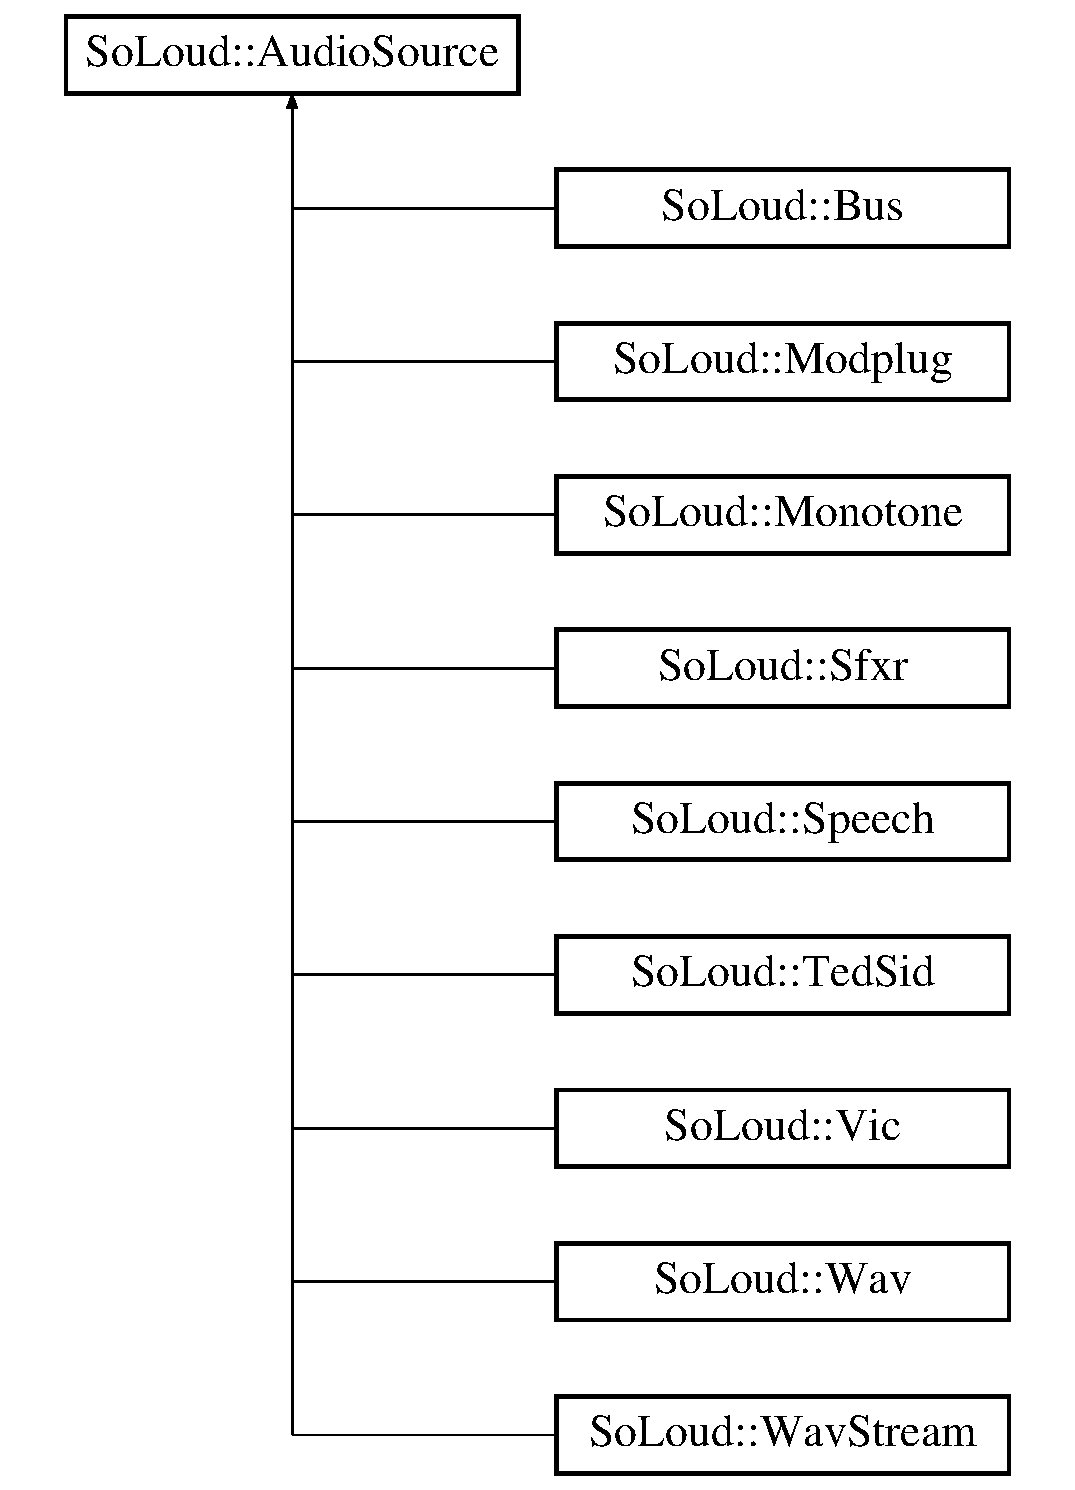
\includegraphics[height=10.000000cm]{class_so_loud_1_1_audio_source}
\end{center}
\end{figure}
\subsection*{Public Types}
\begin{DoxyCompactItemize}
\item 
\mbox{\Hypertarget{class_so_loud_1_1_audio_source_a0c2eb0c2736920eafe2f178a15a5ee3b}\label{class_so_loud_1_1_audio_source_a0c2eb0c2736920eafe2f178a15a5ee3b}} 
enum {\bfseries F\+L\+A\+GS} \{ \newline
{\bfseries S\+H\+O\+U\+L\+D\+\_\+\+L\+O\+OP} = 1, 
{\bfseries S\+I\+N\+G\+L\+E\+\_\+\+I\+N\+S\+T\+A\+N\+CE} = 2, 
{\bfseries V\+I\+S\+U\+A\+L\+I\+Z\+A\+T\+I\+O\+N\+\_\+\+D\+A\+TA} = 4, 
{\bfseries P\+R\+O\+C\+E\+S\+S\+\_\+3D} = 8, 
\newline
{\bfseries L\+I\+S\+T\+E\+N\+E\+R\+\_\+\+R\+E\+L\+A\+T\+I\+VE} = 16, 
{\bfseries D\+I\+S\+T\+A\+N\+C\+E\+\_\+\+D\+E\+L\+AY} = 32, 
{\bfseries I\+N\+A\+U\+D\+I\+B\+L\+E\+\_\+\+K\+I\+LL} = 64, 
{\bfseries I\+N\+A\+U\+D\+I\+B\+L\+E\+\_\+\+T\+I\+CK} = 128
 \}
\item 
\mbox{\Hypertarget{class_so_loud_1_1_audio_source_a8ded5e82ef73b03400178f7cb591b9fb}\label{class_so_loud_1_1_audio_source_a8ded5e82ef73b03400178f7cb591b9fb}} 
enum {\bfseries A\+T\+T\+E\+N\+U\+A\+T\+I\+O\+N\+\_\+\+M\+O\+D\+E\+LS} \{ {\bfseries N\+O\+\_\+\+A\+T\+T\+E\+N\+U\+A\+T\+I\+ON} = 0, 
{\bfseries I\+N\+V\+E\+R\+S\+E\+\_\+\+D\+I\+S\+T\+A\+N\+CE} = 1, 
{\bfseries L\+I\+N\+E\+A\+R\+\_\+\+D\+I\+S\+T\+A\+N\+CE} = 2, 
{\bfseries E\+X\+P\+O\+N\+E\+N\+T\+I\+A\+L\+\_\+\+D\+I\+S\+T\+A\+N\+CE} = 3
 \}
\end{DoxyCompactItemize}
\subsection*{Public Member Functions}
\begin{DoxyCompactItemize}
\item 
\mbox{\Hypertarget{class_so_loud_1_1_audio_source_a131aebb933216574269ce7f394b95b37}\label{class_so_loud_1_1_audio_source_a131aebb933216574269ce7f394b95b37}} 
void {\bfseries set\+Volume} (float a\+Volume)
\item 
\mbox{\Hypertarget{class_so_loud_1_1_audio_source_ad62577bf3b28507cf00fec8122ed3699}\label{class_so_loud_1_1_audio_source_ad62577bf3b28507cf00fec8122ed3699}} 
void {\bfseries set\+Looping} (bool a\+Loop)
\item 
\mbox{\Hypertarget{class_so_loud_1_1_audio_source_a531a9b365bcfcf789f5b7ba187d80379}\label{class_so_loud_1_1_audio_source_a531a9b365bcfcf789f5b7ba187d80379}} 
void {\bfseries set\+Single\+Instance} (bool a\+Single\+Instance)
\item 
\mbox{\Hypertarget{class_so_loud_1_1_audio_source_a2d9daeee1549be617f7e54038296ea1f}\label{class_so_loud_1_1_audio_source_a2d9daeee1549be617f7e54038296ea1f}} 
void {\bfseries set3d\+Min\+Max\+Distance} (float a\+Min\+Distance, float a\+Max\+Distance)
\item 
\mbox{\Hypertarget{class_so_loud_1_1_audio_source_a1c0cee35631865009ab32a30ed5c282c}\label{class_so_loud_1_1_audio_source_a1c0cee35631865009ab32a30ed5c282c}} 
void {\bfseries set3d\+Attenuation} (unsigned int a\+Attenuation\+Model, float a\+Attenuation\+Rolloff\+Factor)
\item 
\mbox{\Hypertarget{class_so_loud_1_1_audio_source_a4dfd2587466142df4d2633ef39f72929}\label{class_so_loud_1_1_audio_source_a4dfd2587466142df4d2633ef39f72929}} 
void {\bfseries set3d\+Doppler\+Factor} (float a\+Doppler\+Factor)
\item 
\mbox{\Hypertarget{class_so_loud_1_1_audio_source_aae197c89ba755873a0fd5bf4ef322ba4}\label{class_so_loud_1_1_audio_source_aae197c89ba755873a0fd5bf4ef322ba4}} 
void {\bfseries set3d\+Processing} (bool a\+Do3d\+Processing)
\item 
\mbox{\Hypertarget{class_so_loud_1_1_audio_source_a886f886e285bc72719c1255409088525}\label{class_so_loud_1_1_audio_source_a886f886e285bc72719c1255409088525}} 
void {\bfseries set3d\+Listener\+Relative} (bool a\+Listener\+Relative)
\item 
\mbox{\Hypertarget{class_so_loud_1_1_audio_source_a669e5d05c0ff5c4e55c6a19ac2660988}\label{class_so_loud_1_1_audio_source_a669e5d05c0ff5c4e55c6a19ac2660988}} 
void {\bfseries set3d\+Distance\+Delay} (bool a\+Distance\+Delay)
\item 
\mbox{\Hypertarget{class_so_loud_1_1_audio_source_a4613f7463b4b8addb2a9e0622b9d4add}\label{class_so_loud_1_1_audio_source_a4613f7463b4b8addb2a9e0622b9d4add}} 
void {\bfseries set3d\+Collider} (\mbox{\hyperlink{class_so_loud_1_1_audio_collider}{Audio\+Collider}} $\ast$a\+Collider, int a\+User\+Data=0)
\item 
\mbox{\Hypertarget{class_so_loud_1_1_audio_source_a39a7ea2b96454986488ce09d4f7f3ff0}\label{class_so_loud_1_1_audio_source_a39a7ea2b96454986488ce09d4f7f3ff0}} 
void {\bfseries set3d\+Attenuator} (\mbox{\hyperlink{class_so_loud_1_1_audio_attenuator}{Audio\+Attenuator}} $\ast$a\+Attenuator)
\item 
\mbox{\Hypertarget{class_so_loud_1_1_audio_source_a692f6985ec2451e6f005e95370e8fd66}\label{class_so_loud_1_1_audio_source_a692f6985ec2451e6f005e95370e8fd66}} 
void {\bfseries set\+Inaudible\+Behavior} (bool a\+Must\+Tick, bool a\+Kill)
\item 
\mbox{\Hypertarget{class_so_loud_1_1_audio_source_afcb0e33e12b051b2746377b0610398a9}\label{class_so_loud_1_1_audio_source_afcb0e33e12b051b2746377b0610398a9}} 
virtual void {\bfseries set\+Filter} (unsigned int a\+Filter\+Id, \mbox{\hyperlink{class_so_loud_1_1_filter}{Filter}} $\ast$a\+Filter)
\item 
\mbox{\Hypertarget{class_so_loud_1_1_audio_source_a998f467f3429af13fd0bcbe9f842ddbe}\label{class_so_loud_1_1_audio_source_a998f467f3429af13fd0bcbe9f842ddbe}} 
virtual \mbox{\hyperlink{class_so_loud_1_1_audio_source_instance}{Audio\+Source\+Instance}} $\ast$ {\bfseries create\+Instance} ()=0
\item 
\mbox{\Hypertarget{class_so_loud_1_1_audio_source_adf861c6b20ed4c2bd318befcd00b3e8b}\label{class_so_loud_1_1_audio_source_adf861c6b20ed4c2bd318befcd00b3e8b}} 
void {\bfseries stop} ()
\end{DoxyCompactItemize}
\subsection*{Public Attributes}
\begin{DoxyCompactItemize}
\item 
\mbox{\Hypertarget{class_so_loud_1_1_audio_source_a6e13c271fa3191061198b8c654a1837f}\label{class_so_loud_1_1_audio_source_a6e13c271fa3191061198b8c654a1837f}} 
unsigned int {\bfseries m\+Flags}
\item 
\mbox{\Hypertarget{class_so_loud_1_1_audio_source_a660554b2372a28101820efe474b2fd5c}\label{class_so_loud_1_1_audio_source_a660554b2372a28101820efe474b2fd5c}} 
float {\bfseries m\+Base\+Samplerate}
\item 
\mbox{\Hypertarget{class_so_loud_1_1_audio_source_ab361882fa4e86dc8771539a3c35e082d}\label{class_so_loud_1_1_audio_source_ab361882fa4e86dc8771539a3c35e082d}} 
float {\bfseries m\+Volume}
\item 
\mbox{\Hypertarget{class_so_loud_1_1_audio_source_aab7ecd88e6aaa429e3d62dd8505c9ec9}\label{class_so_loud_1_1_audio_source_aab7ecd88e6aaa429e3d62dd8505c9ec9}} 
unsigned int {\bfseries m\+Channels}
\item 
\mbox{\Hypertarget{class_so_loud_1_1_audio_source_aa972b38a217a37fef2aa90804b09d322}\label{class_so_loud_1_1_audio_source_aa972b38a217a37fef2aa90804b09d322}} 
unsigned int {\bfseries m\+Audio\+Source\+ID}
\item 
\mbox{\Hypertarget{class_so_loud_1_1_audio_source_adc42ef12c9b72b5e293538def90040ab}\label{class_so_loud_1_1_audio_source_adc42ef12c9b72b5e293538def90040ab}} 
float {\bfseries m3d\+Min\+Distance}
\item 
\mbox{\Hypertarget{class_so_loud_1_1_audio_source_a5386d62281743053560fad27360c0b56}\label{class_so_loud_1_1_audio_source_a5386d62281743053560fad27360c0b56}} 
float {\bfseries m3d\+Max\+Distance}
\item 
\mbox{\Hypertarget{class_so_loud_1_1_audio_source_a9650138a07da450cc4f2af35b43e5cb9}\label{class_so_loud_1_1_audio_source_a9650138a07da450cc4f2af35b43e5cb9}} 
float {\bfseries m3d\+Attenuation\+Rolloff}
\item 
\mbox{\Hypertarget{class_so_loud_1_1_audio_source_a362e3213abca35cbc70062231e2fb307}\label{class_so_loud_1_1_audio_source_a362e3213abca35cbc70062231e2fb307}} 
unsigned int {\bfseries m3d\+Attenuation\+Model}
\item 
\mbox{\Hypertarget{class_so_loud_1_1_audio_source_adf67a122240db629faed56832b101c2c}\label{class_so_loud_1_1_audio_source_adf67a122240db629faed56832b101c2c}} 
float {\bfseries m3d\+Doppler\+Factor}
\item 
\mbox{\Hypertarget{class_so_loud_1_1_audio_source_a294bed8e6837a86dad209b8afdaa79c7}\label{class_so_loud_1_1_audio_source_a294bed8e6837a86dad209b8afdaa79c7}} 
\mbox{\hyperlink{class_so_loud_1_1_filter}{Filter}} $\ast$ {\bfseries m\+Filter} \mbox{[}F\+I\+L\+T\+E\+R\+S\+\_\+\+P\+E\+R\+\_\+\+S\+T\+R\+E\+AM\mbox{]}
\item 
\mbox{\Hypertarget{class_so_loud_1_1_audio_source_afc2e18fdd3f712a2e0a140d0332a89e7}\label{class_so_loud_1_1_audio_source_afc2e18fdd3f712a2e0a140d0332a89e7}} 
\mbox{\hyperlink{class_so_loud_1_1_soloud}{Soloud}} $\ast$ {\bfseries m\+Soloud}
\item 
\mbox{\Hypertarget{class_so_loud_1_1_audio_source_aed2fd77e57a47ed3b32ea94dad48f3ba}\label{class_so_loud_1_1_audio_source_aed2fd77e57a47ed3b32ea94dad48f3ba}} 
\mbox{\hyperlink{class_so_loud_1_1_audio_collider}{Audio\+Collider}} $\ast$ {\bfseries m\+Collider}
\item 
\mbox{\Hypertarget{class_so_loud_1_1_audio_source_a557a1ec3830072cad40be75b4b854861}\label{class_so_loud_1_1_audio_source_a557a1ec3830072cad40be75b4b854861}} 
\mbox{\hyperlink{class_so_loud_1_1_audio_attenuator}{Audio\+Attenuator}} $\ast$ {\bfseries m\+Attenuator}
\item 
\mbox{\Hypertarget{class_so_loud_1_1_audio_source_a4a5224f8ea84fdbbebaebd0064e3911f}\label{class_so_loud_1_1_audio_source_a4a5224f8ea84fdbbebaebd0064e3911f}} 
int {\bfseries m\+Collider\+Data}
\end{DoxyCompactItemize}


The documentation for this class was generated from the following file\+:\begin{DoxyCompactItemize}
\item 
deps/\+E\+S\+A\+T/include/\+E\+S\+A\+T\+\_\+extra/soloud/soloud\+\_\+audiosource.\+h\end{DoxyCompactItemize}

\hypertarget{class_so_loud_1_1_audio_source_instance}{}\section{So\+Loud\+:\+:Audio\+Source\+Instance Class Reference}
\label{class_so_loud_1_1_audio_source_instance}\index{So\+Loud\+::\+Audio\+Source\+Instance@{So\+Loud\+::\+Audio\+Source\+Instance}}
Inheritance diagram for So\+Loud\+:\+:Audio\+Source\+Instance\+:\begin{figure}[H]
\begin{center}
\leavevmode
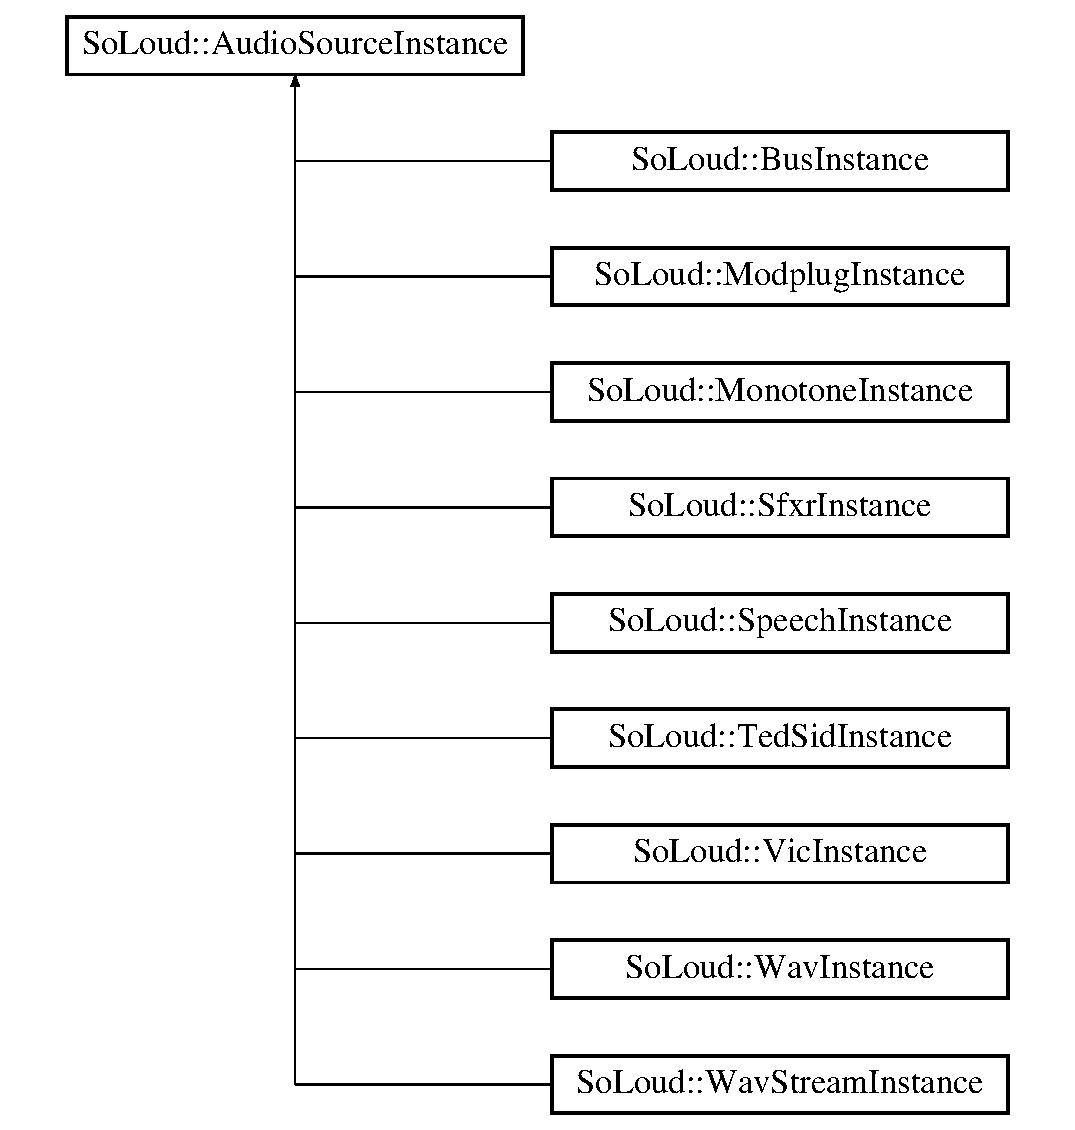
\includegraphics[height=10.000000cm]{class_so_loud_1_1_audio_source_instance}
\end{center}
\end{figure}
\subsection*{Public Types}
\begin{DoxyCompactItemize}
\item 
\mbox{\Hypertarget{class_so_loud_1_1_audio_source_instance_a32c4206e75224bff3a904f300bcccc1d}\label{class_so_loud_1_1_audio_source_instance_a32c4206e75224bff3a904f300bcccc1d}} 
enum {\bfseries F\+L\+A\+GS} \{ \newline
{\bfseries L\+O\+O\+P\+I\+NG} = 1, 
{\bfseries P\+R\+O\+T\+E\+C\+T\+ED} = 2, 
{\bfseries P\+A\+U\+S\+ED} = 4, 
{\bfseries P\+R\+O\+C\+E\+S\+S\+\_\+3D} = 8, 
\newline
{\bfseries L\+I\+S\+T\+E\+N\+E\+R\+\_\+\+R\+E\+L\+A\+T\+I\+VE} = 16, 
{\bfseries I\+N\+A\+U\+D\+I\+B\+LE} = 32, 
{\bfseries I\+N\+A\+U\+D\+I\+B\+L\+E\+\_\+\+K\+I\+LL} = 64, 
{\bfseries I\+N\+A\+U\+D\+I\+B\+L\+E\+\_\+\+T\+I\+CK} = 128
 \}
\end{DoxyCompactItemize}
\subsection*{Public Member Functions}
\begin{DoxyCompactItemize}
\item 
\mbox{\Hypertarget{class_so_loud_1_1_audio_source_instance_aeb5f60467d4cf4837e8dab58569b3ad2}\label{class_so_loud_1_1_audio_source_instance_aeb5f60467d4cf4837e8dab58569b3ad2}} 
void {\bfseries init} (\mbox{\hyperlink{class_so_loud_1_1_audio_source}{Audio\+Source}} \&a\+Source, int a\+Play\+Index)
\item 
\mbox{\Hypertarget{class_so_loud_1_1_audio_source_instance_ab68c5c1b04f75af133740af9121c14d9}\label{class_so_loud_1_1_audio_source_instance_ab68c5c1b04f75af133740af9121c14d9}} 
virtual void {\bfseries get\+Audio} (float $\ast$a\+Buffer, unsigned int a\+Samples)=0
\item 
\mbox{\Hypertarget{class_so_loud_1_1_audio_source_instance_a49b7277a667ff7b49c6e59941f2ee98c}\label{class_so_loud_1_1_audio_source_instance_a49b7277a667ff7b49c6e59941f2ee98c}} 
virtual bool {\bfseries has\+Ended} ()=0
\item 
\mbox{\Hypertarget{class_so_loud_1_1_audio_source_instance_a1ff981495c00ddf75bb1a37d4282e25d}\label{class_so_loud_1_1_audio_source_instance_a1ff981495c00ddf75bb1a37d4282e25d}} 
virtual void {\bfseries seek} (time a\+Seconds, float $\ast$m\+Scratch, unsigned int m\+Scratch\+Size)
\item 
\mbox{\Hypertarget{class_so_loud_1_1_audio_source_instance_a8eb4ca52148ecb9a12c64e4f6a30033f}\label{class_so_loud_1_1_audio_source_instance_a8eb4ca52148ecb9a12c64e4f6a30033f}} 
virtual result {\bfseries rewind} ()
\item 
\mbox{\Hypertarget{class_so_loud_1_1_audio_source_instance_a67872273803ffaccb145da41a2f326cf}\label{class_so_loud_1_1_audio_source_instance_a67872273803ffaccb145da41a2f326cf}} 
virtual float {\bfseries get\+Info} (unsigned int a\+Info\+Key)
\end{DoxyCompactItemize}
\subsection*{Public Attributes}
\begin{DoxyCompactItemize}
\item 
\mbox{\Hypertarget{class_so_loud_1_1_audio_source_instance_a8d5eb5ba50ade05e02f016eee148c512}\label{class_so_loud_1_1_audio_source_instance_a8d5eb5ba50ade05e02f016eee148c512}} 
unsigned int {\bfseries m\+Play\+Index}
\item 
\mbox{\Hypertarget{class_so_loud_1_1_audio_source_instance_a34b4673ae91c521e4429cb2d4121e059}\label{class_so_loud_1_1_audio_source_instance_a34b4673ae91c521e4429cb2d4121e059}} 
unsigned int {\bfseries m\+Loop\+Count}
\item 
\mbox{\Hypertarget{class_so_loud_1_1_audio_source_instance_aa15d49e948ddd05cbbdfe25f205d1af0}\label{class_so_loud_1_1_audio_source_instance_aa15d49e948ddd05cbbdfe25f205d1af0}} 
unsigned int {\bfseries m\+Flags}
\item 
\mbox{\Hypertarget{class_so_loud_1_1_audio_source_instance_aef02eca8fd613d119af8ae7c311d79ac}\label{class_so_loud_1_1_audio_source_instance_aef02eca8fd613d119af8ae7c311d79ac}} 
float {\bfseries m\+Pan}
\item 
\mbox{\Hypertarget{class_so_loud_1_1_audio_source_instance_a6e8448bf071ad5bed2e3c26220acfe7c}\label{class_so_loud_1_1_audio_source_instance_a6e8448bf071ad5bed2e3c26220acfe7c}} 
float {\bfseries m\+Channel\+Volume} \mbox{[}M\+A\+X\+\_\+\+C\+H\+A\+N\+N\+E\+LS\mbox{]}
\item 
\mbox{\Hypertarget{class_so_loud_1_1_audio_source_instance_a2359f806f3920142413236e9b8395be1}\label{class_so_loud_1_1_audio_source_instance_a2359f806f3920142413236e9b8395be1}} 
float {\bfseries m\+Set\+Volume}
\item 
\mbox{\Hypertarget{class_so_loud_1_1_audio_source_instance_a2d7c99990abca8d0fc7cbbef48dfffb0}\label{class_so_loud_1_1_audio_source_instance_a2d7c99990abca8d0fc7cbbef48dfffb0}} 
float {\bfseries m\+Overall\+Volume}
\item 
\mbox{\Hypertarget{class_so_loud_1_1_audio_source_instance_a3acdf7327b08ca150472dc4d71b67fdd}\label{class_so_loud_1_1_audio_source_instance_a3acdf7327b08ca150472dc4d71b67fdd}} 
float {\bfseries m\+Base\+Samplerate}
\item 
\mbox{\Hypertarget{class_so_loud_1_1_audio_source_instance_a8ef707c6d2e9e0a9959dff7b7201684c}\label{class_so_loud_1_1_audio_source_instance_a8ef707c6d2e9e0a9959dff7b7201684c}} 
float {\bfseries m\+Samplerate}
\item 
\mbox{\Hypertarget{class_so_loud_1_1_audio_source_instance_abc7eba521c7cb563ab86a800e8eae1da}\label{class_so_loud_1_1_audio_source_instance_abc7eba521c7cb563ab86a800e8eae1da}} 
unsigned int {\bfseries m\+Channels}
\item 
\mbox{\Hypertarget{class_so_loud_1_1_audio_source_instance_a3537ce61efbe3aedd988bc9f06dc35bf}\label{class_so_loud_1_1_audio_source_instance_a3537ce61efbe3aedd988bc9f06dc35bf}} 
float {\bfseries m\+Set\+Relative\+Play\+Speed}
\item 
\mbox{\Hypertarget{class_so_loud_1_1_audio_source_instance_a0cb11e8db89ce102cccf056d04a91786}\label{class_so_loud_1_1_audio_source_instance_a0cb11e8db89ce102cccf056d04a91786}} 
float {\bfseries m\+Overall\+Relative\+Play\+Speed}
\item 
\mbox{\Hypertarget{class_so_loud_1_1_audio_source_instance_a64b8594ef39d4ab2e1f218eca7799e3b}\label{class_so_loud_1_1_audio_source_instance_a64b8594ef39d4ab2e1f218eca7799e3b}} 
time {\bfseries m\+Stream\+Time}
\item 
\mbox{\Hypertarget{class_so_loud_1_1_audio_source_instance_a6a74ae27e413b17eb14844b960b20c8b}\label{class_so_loud_1_1_audio_source_instance_a6a74ae27e413b17eb14844b960b20c8b}} 
\mbox{\hyperlink{class_so_loud_1_1_fader}{Fader}} {\bfseries m\+Pan\+Fader}
\item 
\mbox{\Hypertarget{class_so_loud_1_1_audio_source_instance_a7439b2234a99e6dcade4fb3fbfbffa23}\label{class_so_loud_1_1_audio_source_instance_a7439b2234a99e6dcade4fb3fbfbffa23}} 
\mbox{\hyperlink{class_so_loud_1_1_fader}{Fader}} {\bfseries m\+Volume\+Fader}
\item 
\mbox{\Hypertarget{class_so_loud_1_1_audio_source_instance_af260f3e8649f3d32ce3b227fd6fda8d9}\label{class_so_loud_1_1_audio_source_instance_af260f3e8649f3d32ce3b227fd6fda8d9}} 
\mbox{\hyperlink{class_so_loud_1_1_fader}{Fader}} {\bfseries m\+Relative\+Play\+Speed\+Fader}
\item 
\mbox{\Hypertarget{class_so_loud_1_1_audio_source_instance_a34c4daae6ac540515b48d797804464d7}\label{class_so_loud_1_1_audio_source_instance_a34c4daae6ac540515b48d797804464d7}} 
\mbox{\hyperlink{class_so_loud_1_1_fader}{Fader}} {\bfseries m\+Pause\+Scheduler}
\item 
\mbox{\Hypertarget{class_so_loud_1_1_audio_source_instance_aa57af3fbb565943a96dcbf5fdd896d01}\label{class_so_loud_1_1_audio_source_instance_aa57af3fbb565943a96dcbf5fdd896d01}} 
\mbox{\hyperlink{class_so_loud_1_1_fader}{Fader}} {\bfseries m\+Stop\+Scheduler}
\item 
\mbox{\Hypertarget{class_so_loud_1_1_audio_source_instance_adb1dc272751b38268aab744ad1eec5bc}\label{class_so_loud_1_1_audio_source_instance_adb1dc272751b38268aab744ad1eec5bc}} 
int {\bfseries m\+Active\+Fader}
\item 
\mbox{\Hypertarget{class_so_loud_1_1_audio_source_instance_a8179d47567eff8b07a714008a0a66a62}\label{class_so_loud_1_1_audio_source_instance_a8179d47567eff8b07a714008a0a66a62}} 
float {\bfseries m\+Current\+Channel\+Volume} \mbox{[}M\+A\+X\+\_\+\+C\+H\+A\+N\+N\+E\+LS\mbox{]}
\item 
\mbox{\Hypertarget{class_so_loud_1_1_audio_source_instance_a2ba43540b8967d86c7fc89bfa0dd3eee}\label{class_so_loud_1_1_audio_source_instance_a2ba43540b8967d86c7fc89bfa0dd3eee}} 
unsigned int {\bfseries m\+Audio\+Source\+ID}
\item 
\mbox{\Hypertarget{class_so_loud_1_1_audio_source_instance_a74029328e5ae36b2b784ff04d9b18acf}\label{class_so_loud_1_1_audio_source_instance_a74029328e5ae36b2b784ff04d9b18acf}} 
unsigned int {\bfseries m\+Bus\+Handle}
\item 
\mbox{\Hypertarget{class_so_loud_1_1_audio_source_instance_a92c5642b02d67061b7e9809a9984c445}\label{class_so_loud_1_1_audio_source_instance_a92c5642b02d67061b7e9809a9984c445}} 
\mbox{\hyperlink{class_so_loud_1_1_filter_instance}{Filter\+Instance}} $\ast$ {\bfseries m\+Filter} \mbox{[}F\+I\+L\+T\+E\+R\+S\+\_\+\+P\+E\+R\+\_\+\+S\+T\+R\+E\+AM\mbox{]}
\item 
\mbox{\Hypertarget{class_so_loud_1_1_audio_source_instance_ae8470a70f90ae5b71170d3855e6b13d8}\label{class_so_loud_1_1_audio_source_instance_ae8470a70f90ae5b71170d3855e6b13d8}} 
\mbox{\hyperlink{struct_so_loud_1_1_audio_source_resample_data}{Audio\+Source\+Resample\+Data}} $\ast$ {\bfseries m\+Resample\+Data} \mbox{[}2\mbox{]}
\item 
\mbox{\Hypertarget{class_so_loud_1_1_audio_source_instance_a41f9ed9f40b5b3602fc335491a0443c2}\label{class_so_loud_1_1_audio_source_instance_a41f9ed9f40b5b3602fc335491a0443c2}} 
unsigned int {\bfseries m\+Src\+Offset}
\item 
\mbox{\Hypertarget{class_so_loud_1_1_audio_source_instance_a77e7ccc37e72c9a5ab812639f7f59dcb}\label{class_so_loud_1_1_audio_source_instance_a77e7ccc37e72c9a5ab812639f7f59dcb}} 
unsigned int {\bfseries m\+Leftover\+Samples}
\item 
\mbox{\Hypertarget{class_so_loud_1_1_audio_source_instance_a326bc9edb5b29c92a6a855a72c3e38f9}\label{class_so_loud_1_1_audio_source_instance_a326bc9edb5b29c92a6a855a72c3e38f9}} 
unsigned int {\bfseries m\+Delay\+Samples}
\end{DoxyCompactItemize}


The documentation for this class was generated from the following file\+:\begin{DoxyCompactItemize}
\item 
deps/\+E\+S\+A\+T/include/\+E\+S\+A\+T\+\_\+extra/soloud/soloud\+\_\+audiosource.\+h\end{DoxyCompactItemize}

\hypertarget{class_so_loud_1_1_audio_source_instance3d_data}{}\section{So\+Loud\+:\+:Audio\+Source\+Instance3d\+Data Class Reference}
\label{class_so_loud_1_1_audio_source_instance3d_data}\index{So\+Loud\+::\+Audio\+Source\+Instance3d\+Data@{So\+Loud\+::\+Audio\+Source\+Instance3d\+Data}}
\subsection*{Public Member Functions}
\begin{DoxyCompactItemize}
\item 
\mbox{\Hypertarget{class_so_loud_1_1_audio_source_instance3d_data_a358f5377c312eb39cf17561a8de71b75}\label{class_so_loud_1_1_audio_source_instance3d_data_a358f5377c312eb39cf17561a8de71b75}} 
void {\bfseries init} (\mbox{\hyperlink{class_so_loud_1_1_audio_source}{Audio\+Source}} \&a\+Source)
\end{DoxyCompactItemize}
\subsection*{Public Attributes}
\begin{DoxyCompactItemize}
\item 
\mbox{\Hypertarget{class_so_loud_1_1_audio_source_instance3d_data_a353bcb0ed79ee1b69ec934671e89e05b}\label{class_so_loud_1_1_audio_source_instance3d_data_a353bcb0ed79ee1b69ec934671e89e05b}} 
float {\bfseries m3d\+Position} \mbox{[}3\mbox{]}
\item 
\mbox{\Hypertarget{class_so_loud_1_1_audio_source_instance3d_data_a440fa5576a4972438a59e03266aba276}\label{class_so_loud_1_1_audio_source_instance3d_data_a440fa5576a4972438a59e03266aba276}} 
float {\bfseries m3d\+Velocity} \mbox{[}3\mbox{]}
\item 
\mbox{\Hypertarget{class_so_loud_1_1_audio_source_instance3d_data_aad31bf0844c655598d7439387032969f}\label{class_so_loud_1_1_audio_source_instance3d_data_aad31bf0844c655598d7439387032969f}} 
float {\bfseries m3d\+Min\+Distance}
\item 
\mbox{\Hypertarget{class_so_loud_1_1_audio_source_instance3d_data_a4bef8c95bf8d3c7f6240f2991b8dfa22}\label{class_so_loud_1_1_audio_source_instance3d_data_a4bef8c95bf8d3c7f6240f2991b8dfa22}} 
float {\bfseries m3d\+Max\+Distance}
\item 
\mbox{\Hypertarget{class_so_loud_1_1_audio_source_instance3d_data_af983f6e13dd950bf9658213a892e60b7}\label{class_so_loud_1_1_audio_source_instance3d_data_af983f6e13dd950bf9658213a892e60b7}} 
float {\bfseries m3d\+Attenuation\+Rolloff}
\item 
\mbox{\Hypertarget{class_so_loud_1_1_audio_source_instance3d_data_a9ef19c4f982efaa9cea6c68c19dbcb69}\label{class_so_loud_1_1_audio_source_instance3d_data_a9ef19c4f982efaa9cea6c68c19dbcb69}} 
unsigned int {\bfseries m3d\+Attenuation\+Model}
\item 
\mbox{\Hypertarget{class_so_loud_1_1_audio_source_instance3d_data_a260fefa5f80a132a80f9fe6983a10e7e}\label{class_so_loud_1_1_audio_source_instance3d_data_a260fefa5f80a132a80f9fe6983a10e7e}} 
float {\bfseries m3d\+Doppler\+Factor}
\item 
\mbox{\Hypertarget{class_so_loud_1_1_audio_source_instance3d_data_af8dbe14ed5dff16c5c7d7d80f478ccc5}\label{class_so_loud_1_1_audio_source_instance3d_data_af8dbe14ed5dff16c5c7d7d80f478ccc5}} 
\mbox{\hyperlink{class_so_loud_1_1_audio_collider}{Audio\+Collider}} $\ast$ {\bfseries m\+Collider}
\item 
\mbox{\Hypertarget{class_so_loud_1_1_audio_source_instance3d_data_aa03eee66c2b601dd2a8a3d25db937476}\label{class_so_loud_1_1_audio_source_instance3d_data_aa03eee66c2b601dd2a8a3d25db937476}} 
\mbox{\hyperlink{class_so_loud_1_1_audio_attenuator}{Audio\+Attenuator}} $\ast$ {\bfseries m\+Attenuator}
\item 
\mbox{\Hypertarget{class_so_loud_1_1_audio_source_instance3d_data_a6234a25705806d11ac592fedf0a23dd1}\label{class_so_loud_1_1_audio_source_instance3d_data_a6234a25705806d11ac592fedf0a23dd1}} 
int {\bfseries m\+Collider\+Data}
\item 
\mbox{\Hypertarget{class_so_loud_1_1_audio_source_instance3d_data_ac80ea416032cf6716fddc475252957bc}\label{class_so_loud_1_1_audio_source_instance3d_data_ac80ea416032cf6716fddc475252957bc}} 
float {\bfseries m\+Doppler\+Value}
\item 
\mbox{\Hypertarget{class_so_loud_1_1_audio_source_instance3d_data_a68c3fd0171ee8236d091215cf3ce8eb8}\label{class_so_loud_1_1_audio_source_instance3d_data_a68c3fd0171ee8236d091215cf3ce8eb8}} 
float {\bfseries m3d\+Volume}
\item 
\mbox{\Hypertarget{class_so_loud_1_1_audio_source_instance3d_data_a7ba2af92eb1802f8a926e1b025ed433f}\label{class_so_loud_1_1_audio_source_instance3d_data_a7ba2af92eb1802f8a926e1b025ed433f}} 
float {\bfseries m\+Channel\+Volume} \mbox{[}M\+A\+X\+\_\+\+C\+H\+A\+N\+N\+E\+LS\mbox{]}
\item 
\mbox{\Hypertarget{class_so_loud_1_1_audio_source_instance3d_data_acebb48b1a0c28291caa8278cf6bb52ea}\label{class_so_loud_1_1_audio_source_instance3d_data_acebb48b1a0c28291caa8278cf6bb52ea}} 
unsigned int {\bfseries m\+Flags}
\item 
\mbox{\Hypertarget{class_so_loud_1_1_audio_source_instance3d_data_a36f1497ab59e11f86125eda3e8b799e8}\label{class_so_loud_1_1_audio_source_instance3d_data_a36f1497ab59e11f86125eda3e8b799e8}} 
handle {\bfseries m\+Handle}
\end{DoxyCompactItemize}


The documentation for this class was generated from the following file\+:\begin{DoxyCompactItemize}
\item 
deps/\+E\+S\+A\+T/include/\+E\+S\+A\+T\+\_\+extra/soloud/soloud\+\_\+audiosource.\+h\end{DoxyCompactItemize}

\hypertarget{struct_so_loud_1_1_audio_source_resample_data}{}\section{So\+Loud\+:\+:Audio\+Source\+Resample\+Data Struct Reference}
\label{struct_so_loud_1_1_audio_source_resample_data}\index{So\+Loud\+::\+Audio\+Source\+Resample\+Data@{So\+Loud\+::\+Audio\+Source\+Resample\+Data}}
\subsection*{Public Attributes}
\begin{DoxyCompactItemize}
\item 
\mbox{\Hypertarget{struct_so_loud_1_1_audio_source_resample_data_ae89072b6507e1f1c898fd9768a38a4d6}\label{struct_so_loud_1_1_audio_source_resample_data_ae89072b6507e1f1c898fd9768a38a4d6}} 
float $\ast$ {\bfseries m\+Buffer}
\end{DoxyCompactItemize}


The documentation for this struct was generated from the following file\+:\begin{DoxyCompactItemize}
\item 
deps/\+E\+S\+A\+T/include/\+E\+S\+A\+T\+\_\+extra/soloud/soloud\+\_\+audiosource.\+h\end{DoxyCompactItemize}

\hypertarget{class_so_loud_1_1_bassboost_filter}{}\section{So\+Loud\+:\+:Bassboost\+Filter Class Reference}
\label{class_so_loud_1_1_bassboost_filter}\index{So\+Loud\+::\+Bassboost\+Filter@{So\+Loud\+::\+Bassboost\+Filter}}
Inheritance diagram for So\+Loud\+:\+:Bassboost\+Filter\+:\begin{figure}[H]
\begin{center}
\leavevmode
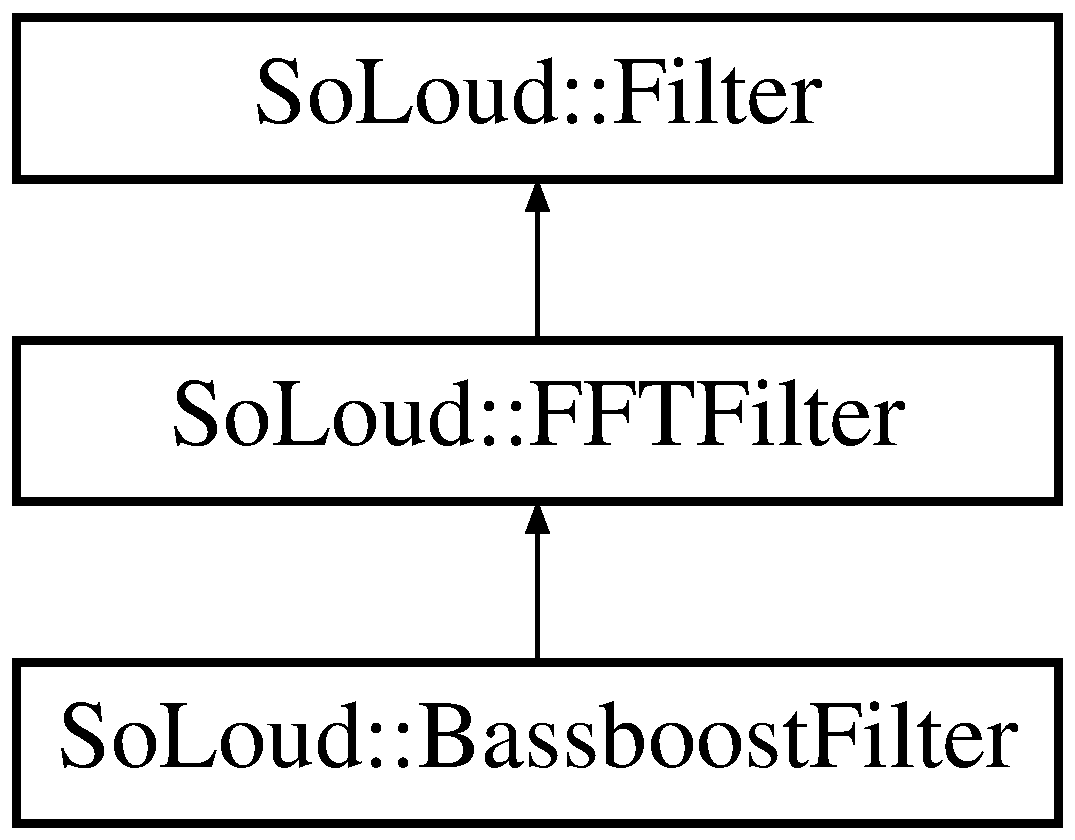
\includegraphics[height=3.000000cm]{class_so_loud_1_1_bassboost_filter}
\end{center}
\end{figure}
\subsection*{Public Types}
\begin{DoxyCompactItemize}
\item 
\mbox{\Hypertarget{class_so_loud_1_1_bassboost_filter_a7b75a38ff566a9e470f7404aec931547}\label{class_so_loud_1_1_bassboost_filter_a7b75a38ff566a9e470f7404aec931547}} 
enum {\bfseries F\+I\+L\+T\+E\+R\+A\+T\+T\+R\+I\+B\+U\+TE} \{ {\bfseries W\+ET} = 0, 
{\bfseries B\+O\+O\+ST} = 1
 \}
\end{DoxyCompactItemize}
\subsection*{Public Member Functions}
\begin{DoxyCompactItemize}
\item 
\mbox{\Hypertarget{class_so_loud_1_1_bassboost_filter_aded072ee3842f0f8870b5e24cc6bf94d}\label{class_so_loud_1_1_bassboost_filter_aded072ee3842f0f8870b5e24cc6bf94d}} 
result {\bfseries set\+Params} (float a\+Boost)
\item 
\mbox{\Hypertarget{class_so_loud_1_1_bassboost_filter_a8577039204f428e7fc881fd2649b5f0c}\label{class_so_loud_1_1_bassboost_filter_a8577039204f428e7fc881fd2649b5f0c}} 
virtual \mbox{\hyperlink{class_so_loud_1_1_filter_instance}{Filter\+Instance}} $\ast$ {\bfseries create\+Instance} ()
\end{DoxyCompactItemize}
\subsection*{Public Attributes}
\begin{DoxyCompactItemize}
\item 
\mbox{\Hypertarget{class_so_loud_1_1_bassboost_filter_aad8ee489ea88a5fd2bf767205135a1f4}\label{class_so_loud_1_1_bassboost_filter_aad8ee489ea88a5fd2bf767205135a1f4}} 
float {\bfseries m\+Boost}
\end{DoxyCompactItemize}


The documentation for this class was generated from the following file\+:\begin{DoxyCompactItemize}
\item 
deps/\+E\+S\+A\+T/include/\+E\+S\+A\+T\+\_\+extra/soloud/soloud\+\_\+bassboostfilter.\+h\end{DoxyCompactItemize}

\hypertarget{class_so_loud_1_1_bassboost_filter_instance}{}\section{So\+Loud\+:\+:Bassboost\+Filter\+Instance Class Reference}
\label{class_so_loud_1_1_bassboost_filter_instance}\index{So\+Loud\+::\+Bassboost\+Filter\+Instance@{So\+Loud\+::\+Bassboost\+Filter\+Instance}}
Inheritance diagram for So\+Loud\+:\+:Bassboost\+Filter\+Instance\+:\begin{figure}[H]
\begin{center}
\leavevmode
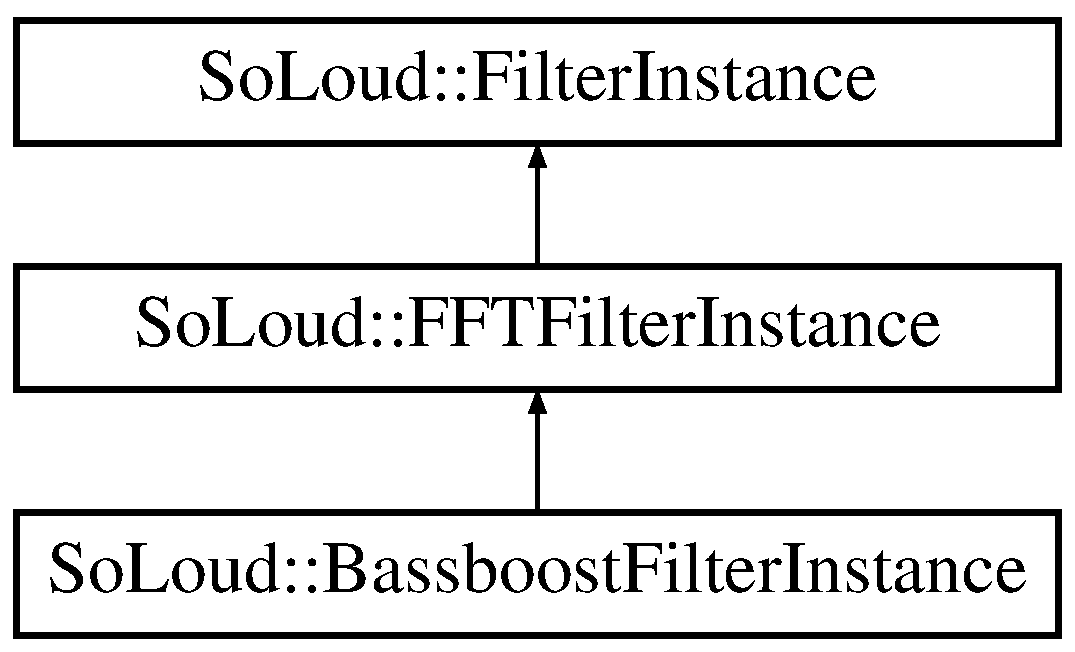
\includegraphics[height=3.000000cm]{class_so_loud_1_1_bassboost_filter_instance}
\end{center}
\end{figure}
\subsection*{Public Member Functions}
\begin{DoxyCompactItemize}
\item 
\mbox{\Hypertarget{class_so_loud_1_1_bassboost_filter_instance_a8e7c282c5e6fbe5220007a7d471d65a8}\label{class_so_loud_1_1_bassboost_filter_instance_a8e7c282c5e6fbe5220007a7d471d65a8}} 
virtual void {\bfseries fft\+Filter\+Channel} (float $\ast$a\+F\+F\+T\+Buffer, unsigned int a\+Samples, float a\+Samplerate, time a\+Time, unsigned int a\+Channel, unsigned int a\+Channels)
\item 
\mbox{\Hypertarget{class_so_loud_1_1_bassboost_filter_instance_a3f96f0c9adbb5aba9cfe37a2585607cf}\label{class_so_loud_1_1_bassboost_filter_instance_a3f96f0c9adbb5aba9cfe37a2585607cf}} 
{\bfseries Bassboost\+Filter\+Instance} (\mbox{\hyperlink{class_so_loud_1_1_bassboost_filter}{Bassboost\+Filter}} $\ast$a\+Parent)
\end{DoxyCompactItemize}
\subsection*{Additional Inherited Members}


The documentation for this class was generated from the following file\+:\begin{DoxyCompactItemize}
\item 
deps/\+E\+S\+A\+T/include/\+E\+S\+A\+T\+\_\+extra/soloud/soloud\+\_\+bassboostfilter.\+h\end{DoxyCompactItemize}

\hypertarget{class_so_loud_1_1_biquad_resonant_filter}{}\section{So\+Loud\+:\+:Biquad\+Resonant\+Filter Class Reference}
\label{class_so_loud_1_1_biquad_resonant_filter}\index{So\+Loud\+::\+Biquad\+Resonant\+Filter@{So\+Loud\+::\+Biquad\+Resonant\+Filter}}
Inheritance diagram for So\+Loud\+:\+:Biquad\+Resonant\+Filter\+:\begin{figure}[H]
\begin{center}
\leavevmode
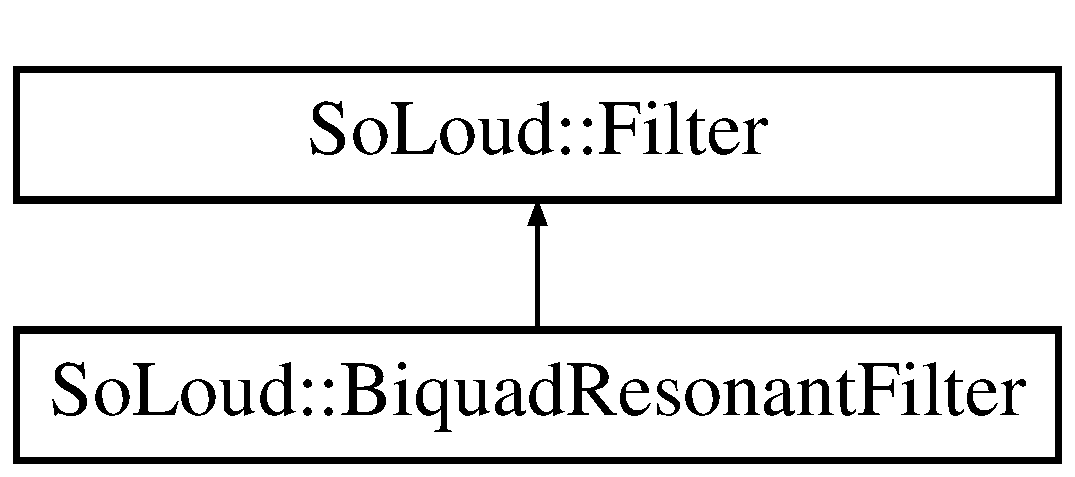
\includegraphics[height=2.000000cm]{class_so_loud_1_1_biquad_resonant_filter}
\end{center}
\end{figure}
\subsection*{Public Types}
\begin{DoxyCompactItemize}
\item 
\mbox{\Hypertarget{class_so_loud_1_1_biquad_resonant_filter_a0f24bc97c3d6f6eb215be8e44c484071}\label{class_so_loud_1_1_biquad_resonant_filter_a0f24bc97c3d6f6eb215be8e44c484071}} 
enum {\bfseries F\+I\+L\+T\+E\+R\+T\+Y\+PE} \{ {\bfseries N\+O\+NE} = 0, 
{\bfseries L\+O\+W\+P\+A\+SS} = 1, 
{\bfseries H\+I\+G\+H\+P\+A\+SS} = 2, 
{\bfseries B\+A\+N\+D\+P\+A\+SS} = 3
 \}
\item 
\mbox{\Hypertarget{class_so_loud_1_1_biquad_resonant_filter_a50ed3775c10fd396de47dfd0df63f09d}\label{class_so_loud_1_1_biquad_resonant_filter_a50ed3775c10fd396de47dfd0df63f09d}} 
enum {\bfseries F\+I\+L\+T\+E\+R\+A\+T\+T\+R\+I\+B\+U\+TE} \{ {\bfseries W\+ET} = 0, 
{\bfseries S\+A\+M\+P\+L\+E\+R\+A\+TE} = 1, 
{\bfseries F\+R\+E\+Q\+U\+E\+N\+CY} = 2, 
{\bfseries R\+E\+S\+O\+N\+A\+N\+CE} = 3
 \}
\end{DoxyCompactItemize}
\subsection*{Public Member Functions}
\begin{DoxyCompactItemize}
\item 
\mbox{\Hypertarget{class_so_loud_1_1_biquad_resonant_filter_aebe5dbf06e16fcc56eab973d12dc3eaa}\label{class_so_loud_1_1_biquad_resonant_filter_aebe5dbf06e16fcc56eab973d12dc3eaa}} 
virtual \mbox{\hyperlink{class_so_loud_1_1_biquad_resonant_filter_instance}{Biquad\+Resonant\+Filter\+Instance}} $\ast$ {\bfseries create\+Instance} ()
\item 
\mbox{\Hypertarget{class_so_loud_1_1_biquad_resonant_filter_afb351a0c26dc8f56d4bc165d922c703b}\label{class_so_loud_1_1_biquad_resonant_filter_afb351a0c26dc8f56d4bc165d922c703b}} 
result {\bfseries set\+Params} (int a\+Type, float a\+Sample\+Rate, float a\+Frequency, float a\+Resonance)
\end{DoxyCompactItemize}
\subsection*{Public Attributes}
\begin{DoxyCompactItemize}
\item 
\mbox{\Hypertarget{class_so_loud_1_1_biquad_resonant_filter_a50e3f094f703e4c2780dc935d34ee3b7}\label{class_so_loud_1_1_biquad_resonant_filter_a50e3f094f703e4c2780dc935d34ee3b7}} 
int {\bfseries m\+Filter\+Type}
\item 
\mbox{\Hypertarget{class_so_loud_1_1_biquad_resonant_filter_af4172c10d05c58af54299a0bc586b706}\label{class_so_loud_1_1_biquad_resonant_filter_af4172c10d05c58af54299a0bc586b706}} 
float {\bfseries m\+Sample\+Rate}
\item 
\mbox{\Hypertarget{class_so_loud_1_1_biquad_resonant_filter_a4a87bf863804bb3a9cd0a09cc0db00b3}\label{class_so_loud_1_1_biquad_resonant_filter_a4a87bf863804bb3a9cd0a09cc0db00b3}} 
float {\bfseries m\+Frequency}
\item 
\mbox{\Hypertarget{class_so_loud_1_1_biquad_resonant_filter_a06f7f1c568237c23b9d05fd7695d3a63}\label{class_so_loud_1_1_biquad_resonant_filter_a06f7f1c568237c23b9d05fd7695d3a63}} 
float {\bfseries m\+Resonance}
\end{DoxyCompactItemize}


The documentation for this class was generated from the following file\+:\begin{DoxyCompactItemize}
\item 
deps/\+E\+S\+A\+T/include/\+E\+S\+A\+T\+\_\+extra/soloud/soloud\+\_\+biquadresonantfilter.\+h\end{DoxyCompactItemize}

\hypertarget{class_so_loud_1_1_biquad_resonant_filter_instance}{}\section{So\+Loud\+:\+:Biquad\+Resonant\+Filter\+Instance Class Reference}
\label{class_so_loud_1_1_biquad_resonant_filter_instance}\index{So\+Loud\+::\+Biquad\+Resonant\+Filter\+Instance@{So\+Loud\+::\+Biquad\+Resonant\+Filter\+Instance}}
Inheritance diagram for So\+Loud\+:\+:Biquad\+Resonant\+Filter\+Instance\+:\begin{figure}[H]
\begin{center}
\leavevmode
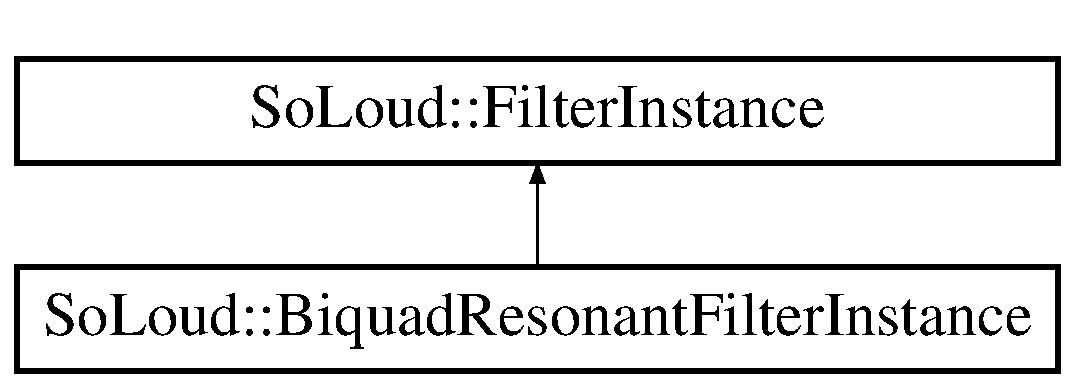
\includegraphics[height=2.000000cm]{class_so_loud_1_1_biquad_resonant_filter_instance}
\end{center}
\end{figure}
\subsection*{Public Member Functions}
\begin{DoxyCompactItemize}
\item 
\mbox{\Hypertarget{class_so_loud_1_1_biquad_resonant_filter_instance_acc516edf0a69500fd6d297cab6717a98}\label{class_so_loud_1_1_biquad_resonant_filter_instance_acc516edf0a69500fd6d297cab6717a98}} 
virtual void {\bfseries filter\+Channel} (float $\ast$a\+Buffer, unsigned int a\+Samples, float a\+Samplerate, time a\+Time, unsigned int a\+Channel, unsigned int a\+Channels)
\item 
\mbox{\Hypertarget{class_so_loud_1_1_biquad_resonant_filter_instance_a2261a84c040a0ab189fb631a6dc87ab0}\label{class_so_loud_1_1_biquad_resonant_filter_instance_a2261a84c040a0ab189fb631a6dc87ab0}} 
{\bfseries Biquad\+Resonant\+Filter\+Instance} (\mbox{\hyperlink{class_so_loud_1_1_biquad_resonant_filter}{Biquad\+Resonant\+Filter}} $\ast$a\+Parent)
\end{DoxyCompactItemize}
\subsection*{Additional Inherited Members}


The documentation for this class was generated from the following file\+:\begin{DoxyCompactItemize}
\item 
deps/\+E\+S\+A\+T/include/\+E\+S\+A\+T\+\_\+extra/soloud/soloud\+\_\+biquadresonantfilter.\+h\end{DoxyCompactItemize}

\hypertarget{struct_so_loud_1_1_b_q_r_state_data}{}\section{So\+Loud\+:\+:B\+Q\+R\+State\+Data Struct Reference}
\label{struct_so_loud_1_1_b_q_r_state_data}\index{So\+Loud\+::\+B\+Q\+R\+State\+Data@{So\+Loud\+::\+B\+Q\+R\+State\+Data}}
\subsection*{Public Attributes}
\begin{DoxyCompactItemize}
\item 
\mbox{\Hypertarget{struct_so_loud_1_1_b_q_r_state_data_a80b0ecee8f145458a18168971bcbf88d}\label{struct_so_loud_1_1_b_q_r_state_data_a80b0ecee8f145458a18168971bcbf88d}} 
float {\bfseries m\+Y1}
\item 
\mbox{\Hypertarget{struct_so_loud_1_1_b_q_r_state_data_a143a6664fd0bb1a4d1be9b53796bf93c}\label{struct_so_loud_1_1_b_q_r_state_data_a143a6664fd0bb1a4d1be9b53796bf93c}} 
float {\bfseries m\+Y2}
\item 
\mbox{\Hypertarget{struct_so_loud_1_1_b_q_r_state_data_ae5f9b17ba8305d7ef6e07fc682aea939}\label{struct_so_loud_1_1_b_q_r_state_data_ae5f9b17ba8305d7ef6e07fc682aea939}} 
float {\bfseries m\+X1}
\item 
\mbox{\Hypertarget{struct_so_loud_1_1_b_q_r_state_data_ae614479ecebade22c1a941e1a2fbe6b0}\label{struct_so_loud_1_1_b_q_r_state_data_ae614479ecebade22c1a941e1a2fbe6b0}} 
float {\bfseries m\+X2}
\end{DoxyCompactItemize}


The documentation for this struct was generated from the following file\+:\begin{DoxyCompactItemize}
\item 
deps/\+E\+S\+A\+T/include/\+E\+S\+A\+T\+\_\+extra/soloud/soloud\+\_\+biquadresonantfilter.\+h\end{DoxyCompactItemize}

\hypertarget{class_so_loud_1_1_bus}{}\section{So\+Loud\+:\+:Bus Class Reference}
\label{class_so_loud_1_1_bus}\index{So\+Loud\+::\+Bus@{So\+Loud\+::\+Bus}}
Inheritance diagram for So\+Loud\+:\+:Bus\+:\begin{figure}[H]
\begin{center}
\leavevmode
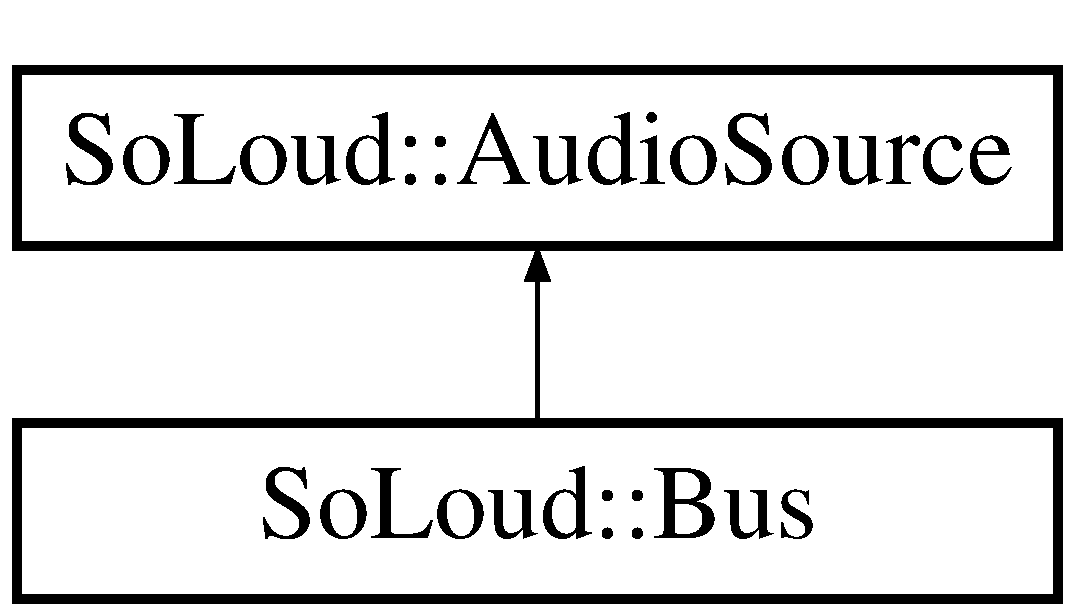
\includegraphics[height=2.000000cm]{class_so_loud_1_1_bus}
\end{center}
\end{figure}
\subsection*{Public Member Functions}
\begin{DoxyCompactItemize}
\item 
\mbox{\Hypertarget{class_so_loud_1_1_bus_a46f89ce122e732a105382d01415dcf15}\label{class_so_loud_1_1_bus_a46f89ce122e732a105382d01415dcf15}} 
virtual \mbox{\hyperlink{class_so_loud_1_1_bus_instance}{Bus\+Instance}} $\ast$ {\bfseries create\+Instance} ()
\item 
\mbox{\Hypertarget{class_so_loud_1_1_bus_adc155188e09e9d5bebe0b151815b3ac0}\label{class_so_loud_1_1_bus_adc155188e09e9d5bebe0b151815b3ac0}} 
virtual void {\bfseries set\+Filter} (unsigned int a\+Filter\+Id, \mbox{\hyperlink{class_so_loud_1_1_filter}{Filter}} $\ast$a\+Filter)
\item 
\mbox{\Hypertarget{class_so_loud_1_1_bus_a9fed9a7b746fda44b9212471c9a2f4d4}\label{class_so_loud_1_1_bus_a9fed9a7b746fda44b9212471c9a2f4d4}} 
handle {\bfseries play} (\mbox{\hyperlink{class_so_loud_1_1_audio_source}{Audio\+Source}} \&a\+Sound, float a\+Volume=1.\+0f, float a\+Pan=0.\+0f, bool a\+Paused=0)
\item 
\mbox{\Hypertarget{class_so_loud_1_1_bus_ad42e5cb151a2eececa8fb5e7d14a7669}\label{class_so_loud_1_1_bus_ad42e5cb151a2eececa8fb5e7d14a7669}} 
handle {\bfseries play\+Clocked} (time a\+Sound\+Time, \mbox{\hyperlink{class_so_loud_1_1_audio_source}{Audio\+Source}} \&a\+Sound, float a\+Volume=1.\+0f, float a\+Pan=0.\+0f)
\item 
\mbox{\Hypertarget{class_so_loud_1_1_bus_a3469af79377fcf6d803351f81a3c9e58}\label{class_so_loud_1_1_bus_a3469af79377fcf6d803351f81a3c9e58}} 
handle {\bfseries play3d} (\mbox{\hyperlink{class_so_loud_1_1_audio_source}{Audio\+Source}} \&a\+Sound, float a\+PosX, float a\+PosY, float a\+PosZ, float a\+VelX=0.\+0f, float a\+Vel\+Y=0.\+0f, float a\+Vel\+Z=0.\+0f, float a\+Volume=1.\+0f, bool a\+Paused=0)
\item 
\mbox{\Hypertarget{class_so_loud_1_1_bus_ab660cf763eb4a68be97d7539d6893952}\label{class_so_loud_1_1_bus_ab660cf763eb4a68be97d7539d6893952}} 
handle {\bfseries play3d\+Clocked} (time a\+Sound\+Time, \mbox{\hyperlink{class_so_loud_1_1_audio_source}{Audio\+Source}} \&a\+Sound, float a\+PosX, float a\+PosY, float a\+PosZ, float a\+VelX=0.\+0f, float a\+Vel\+Y=0.\+0f, float a\+Vel\+Z=0.\+0f, float a\+Volume=1.\+0f)
\item 
\mbox{\Hypertarget{class_so_loud_1_1_bus_a3981391bb38f3356fdb329124c398750}\label{class_so_loud_1_1_bus_a3981391bb38f3356fdb329124c398750}} 
result {\bfseries set\+Channels} (unsigned int a\+Channels)
\item 
\mbox{\Hypertarget{class_so_loud_1_1_bus_a4367e7475af9b3bd5959dc103fd30e21}\label{class_so_loud_1_1_bus_a4367e7475af9b3bd5959dc103fd30e21}} 
void {\bfseries set\+Visualization\+Enable} (bool a\+Enable)
\item 
\mbox{\Hypertarget{class_so_loud_1_1_bus_a22ff3334affcd26edb50d899da24224c}\label{class_so_loud_1_1_bus_a22ff3334affcd26edb50d899da24224c}} 
float $\ast$ {\bfseries calc\+F\+FT} ()
\item 
\mbox{\Hypertarget{class_so_loud_1_1_bus_a77dae82a61fcf934cb46572bda01f34f}\label{class_so_loud_1_1_bus_a77dae82a61fcf934cb46572bda01f34f}} 
float $\ast$ {\bfseries get\+Wave} ()
\item 
\mbox{\Hypertarget{class_so_loud_1_1_bus_a171589a229eab854123bf6f88086a5d1}\label{class_so_loud_1_1_bus_a171589a229eab854123bf6f88086a5d1}} 
void {\bfseries find\+Bus\+Handle} ()
\end{DoxyCompactItemize}
\subsection*{Public Attributes}
\begin{DoxyCompactItemize}
\item 
\mbox{\Hypertarget{class_so_loud_1_1_bus_aa4b3c29a794cfe468d6871f69a1f8e92}\label{class_so_loud_1_1_bus_aa4b3c29a794cfe468d6871f69a1f8e92}} 
\mbox{\hyperlink{class_so_loud_1_1_bus_instance}{Bus\+Instance}} $\ast$ {\bfseries m\+Instance}
\item 
\mbox{\Hypertarget{class_so_loud_1_1_bus_a0e5ce0894c817cdd158922989bde0387}\label{class_so_loud_1_1_bus_a0e5ce0894c817cdd158922989bde0387}} 
unsigned int {\bfseries m\+Channel\+Handle}
\item 
\mbox{\Hypertarget{class_so_loud_1_1_bus_a38a6d2c789a33659f07dd911b93327e3}\label{class_so_loud_1_1_bus_a38a6d2c789a33659f07dd911b93327e3}} 
float {\bfseries m\+F\+F\+T\+Data} \mbox{[}256\mbox{]}
\item 
\mbox{\Hypertarget{class_so_loud_1_1_bus_a722292f1f9cb03c851497a5e9cd9f551}\label{class_so_loud_1_1_bus_a722292f1f9cb03c851497a5e9cd9f551}} 
float {\bfseries m\+Wave\+Data} \mbox{[}256\mbox{]}
\end{DoxyCompactItemize}
\subsection*{Additional Inherited Members}


The documentation for this class was generated from the following file\+:\begin{DoxyCompactItemize}
\item 
deps/\+E\+S\+A\+T/include/\+E\+S\+A\+T\+\_\+extra/soloud/soloud\+\_\+bus.\+h\end{DoxyCompactItemize}

\hypertarget{class_so_loud_1_1_bus_instance}{}\section{So\+Loud\+:\+:Bus\+Instance Class Reference}
\label{class_so_loud_1_1_bus_instance}\index{So\+Loud\+::\+Bus\+Instance@{So\+Loud\+::\+Bus\+Instance}}
Inheritance diagram for So\+Loud\+:\+:Bus\+Instance\+:\begin{figure}[H]
\begin{center}
\leavevmode
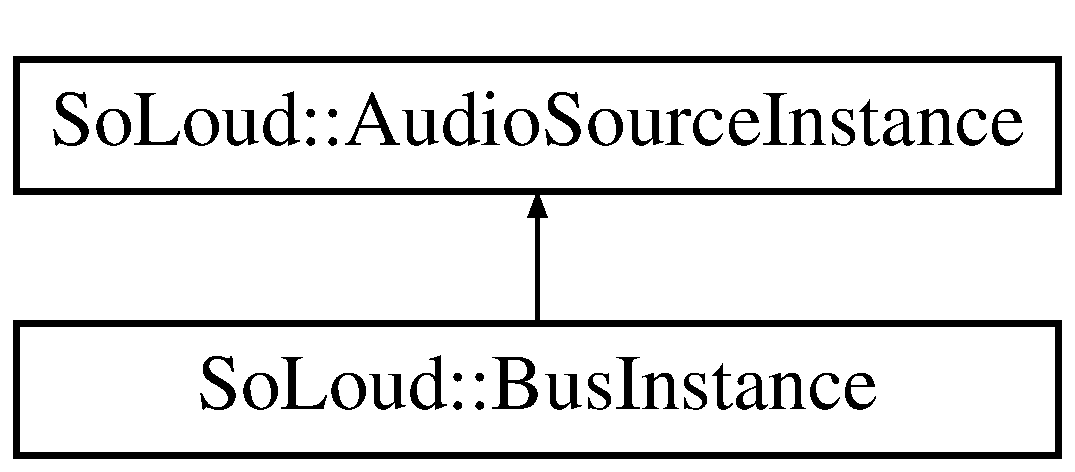
\includegraphics[height=2.000000cm]{class_so_loud_1_1_bus_instance}
\end{center}
\end{figure}
\subsection*{Public Member Functions}
\begin{DoxyCompactItemize}
\item 
\mbox{\Hypertarget{class_so_loud_1_1_bus_instance_a4bd198344ac6013b8814d6d5a199a39e}\label{class_so_loud_1_1_bus_instance_a4bd198344ac6013b8814d6d5a199a39e}} 
{\bfseries Bus\+Instance} (\mbox{\hyperlink{class_so_loud_1_1_bus}{Bus}} $\ast$a\+Parent)
\item 
\mbox{\Hypertarget{class_so_loud_1_1_bus_instance_abb28a81c6c19a528852db281178521ab}\label{class_so_loud_1_1_bus_instance_abb28a81c6c19a528852db281178521ab}} 
virtual void {\bfseries get\+Audio} (float $\ast$a\+Buffer, unsigned int a\+Samples)
\item 
\mbox{\Hypertarget{class_so_loud_1_1_bus_instance_ab8f4d736266bc1d0503a46a9793f824b}\label{class_so_loud_1_1_bus_instance_ab8f4d736266bc1d0503a46a9793f824b}} 
virtual bool {\bfseries has\+Ended} ()
\end{DoxyCompactItemize}
\subsection*{Public Attributes}
\begin{DoxyCompactItemize}
\item 
\mbox{\Hypertarget{class_so_loud_1_1_bus_instance_a02aa0be39eec9ce8986dbc6e0bc87e2b}\label{class_so_loud_1_1_bus_instance_a02aa0be39eec9ce8986dbc6e0bc87e2b}} 
float {\bfseries m\+Visualization\+Wave\+Data} \mbox{[}256\mbox{]}
\end{DoxyCompactItemize}
\subsection*{Additional Inherited Members}


The documentation for this class was generated from the following file\+:\begin{DoxyCompactItemize}
\item 
deps/\+E\+S\+A\+T/include/\+E\+S\+A\+T\+\_\+extra/soloud/soloud\+\_\+bus.\+h\end{DoxyCompactItemize}

\hypertarget{structcp_arbiter}{}\section{cp\+Arbiter Struct Reference}
\label{structcp_arbiter}\index{cp\+Arbiter@{cp\+Arbiter}}
\subsection*{Public Attributes}
\begin{DoxyCompactItemize}
\item 
\mbox{\Hypertarget{structcp_arbiter_ae28e688fb03eba42a1dd786ab914c9eb}\label{structcp_arbiter_ae28e688fb03eba42a1dd786ab914c9eb}} 
\mbox{\hyperlink{group__basic_types_gac1ed65573e035bf892505768c852d8d3}{cp\+Float}} {\bfseries e}
\item 
\mbox{\Hypertarget{structcp_arbiter_a1be4918be41986330005a6e745d013f3}\label{structcp_arbiter_a1be4918be41986330005a6e745d013f3}} 
\mbox{\hyperlink{group__basic_types_gac1ed65573e035bf892505768c852d8d3}{cp\+Float}} {\bfseries u}
\item 
\mbox{\Hypertarget{structcp_arbiter_ad8724ab2c97ec732128fafc77668cc54}\label{structcp_arbiter_ad8724ab2c97ec732128fafc77668cc54}} 
\mbox{\hyperlink{structcp_vect}{cp\+Vect}} {\bfseries surface\+\_\+vr}
\item 
\mbox{\Hypertarget{structcp_arbiter_afb41ae8c3e4df711f47ab7ac3ef7ed9a}\label{structcp_arbiter_afb41ae8c3e4df711f47ab7ac3ef7ed9a}} 
\mbox{\hyperlink{group__basic_types_ga2ac2c3c31e21893941f9e4f8ee279447}{cp\+Data\+Pointer}} {\bfseries data}
\item 
\mbox{\Hypertarget{structcp_arbiter_a169358f50db550583803f105df13ae48}\label{structcp_arbiter_a169358f50db550583803f105df13ae48}} 
const \mbox{\hyperlink{structcp_shape}{cp\+Shape}} $\ast$ {\bfseries a}
\item 
\mbox{\Hypertarget{structcp_arbiter_a0609639e649ef29acf5f5aaeb26d2036}\label{structcp_arbiter_a0609639e649ef29acf5f5aaeb26d2036}} 
const \mbox{\hyperlink{structcp_shape}{cp\+Shape}} $\ast$ {\bfseries b}
\item 
\mbox{\Hypertarget{structcp_arbiter_a0e310136b1a4d5b46a374b35fcd49f62}\label{structcp_arbiter_a0e310136b1a4d5b46a374b35fcd49f62}} 
\mbox{\hyperlink{structcp_body}{cp\+Body}} $\ast$ {\bfseries body\+\_\+a}
\item 
\mbox{\Hypertarget{structcp_arbiter_a07ad23b13b383a3fd3e4834865ad4b50}\label{structcp_arbiter_a07ad23b13b383a3fd3e4834865ad4b50}} 
\mbox{\hyperlink{structcp_body}{cp\+Body}} $\ast$ {\bfseries body\+\_\+b}
\item 
\mbox{\Hypertarget{structcp_arbiter_a33883f0931febf9b4111c0f795834b4f}\label{structcp_arbiter_a33883f0931febf9b4111c0f795834b4f}} 
struct \mbox{\hyperlink{structcp_arbiter_thread}{cp\+Arbiter\+Thread}} thread\+\_\+a {\bfseries thread\+\_\+b}
\item 
\mbox{\Hypertarget{structcp_arbiter_a7dfee6fde35d7bb551ee24fcbbe49018}\label{structcp_arbiter_a7dfee6fde35d7bb551ee24fcbbe49018}} 
int {\bfseries count}
\item 
\mbox{\Hypertarget{structcp_arbiter_a4654107db135771ba090750bbadec376}\label{structcp_arbiter_a4654107db135771ba090750bbadec376}} 
struct \mbox{\hyperlink{structcp_contact}{cp\+Contact}} $\ast$ {\bfseries contacts}
\item 
\mbox{\Hypertarget{structcp_arbiter_a74be8aab017a21f5a2ff1dd1a233a3b3}\label{structcp_arbiter_a74be8aab017a21f5a2ff1dd1a233a3b3}} 
\mbox{\hyperlink{structcp_vect}{cp\+Vect}} {\bfseries n}
\item 
\mbox{\Hypertarget{structcp_arbiter_a0bf89f22d68c4892b26702b4d8a1ee04}\label{structcp_arbiter_a0bf89f22d68c4892b26702b4d8a1ee04}} 
\mbox{\hyperlink{structcp_collision_handler}{cp\+Collision\+Handler}} $\ast$ {\bfseries handler}
\item 
\mbox{\Hypertarget{structcp_arbiter_aa089aee327ce057cbbd7868403a929e4}\label{structcp_arbiter_aa089aee327ce057cbbd7868403a929e4}} 
\mbox{\hyperlink{structcp_collision_handler}{cp\+Collision\+Handler}} $\ast$ {\bfseries handlerA}
\item 
\mbox{\Hypertarget{structcp_arbiter_aa983a7ae64a50b5ca095a47605379e4a}\label{structcp_arbiter_aa983a7ae64a50b5ca095a47605379e4a}} 
\mbox{\hyperlink{structcp_collision_handler}{cp\+Collision\+Handler}} $\ast$ {\bfseries handlerB}
\item 
\mbox{\Hypertarget{structcp_arbiter_a05eb6f37d1e8b27dcfbccd79d5773495}\label{structcp_arbiter_a05eb6f37d1e8b27dcfbccd79d5773495}} 
\mbox{\hyperlink{group__basic_types_gabc5e752c48f3449ca26ef413ecbd647e}{cp\+Bool}} {\bfseries swapped}
\item 
\mbox{\Hypertarget{structcp_arbiter_a7c724b956f3d7b91f6aa1d73d886b56c}\label{structcp_arbiter_a7c724b956f3d7b91f6aa1d73d886b56c}} 
\mbox{\hyperlink{group__basic_types_gaa24652c104082d0725066ea5ac7dc83f}{cp\+Timestamp}} {\bfseries stamp}
\item 
\mbox{\Hypertarget{structcp_arbiter_a972953b321f437fbc5000539cc7e3b1e}\label{structcp_arbiter_a972953b321f437fbc5000539cc7e3b1e}} 
enum cp\+Arbiter\+State {\bfseries state}
\end{DoxyCompactItemize}


The documentation for this struct was generated from the following file\+:\begin{DoxyCompactItemize}
\item 
deps/\+E\+S\+A\+T/include/\+E\+S\+A\+T\+\_\+extra/chipmunk/chipmunk\+\_\+private.\+h\end{DoxyCompactItemize}

\hypertarget{structcp_arbiter_thread}{}\section{cp\+Arbiter\+Thread Struct Reference}
\label{structcp_arbiter_thread}\index{cp\+Arbiter\+Thread@{cp\+Arbiter\+Thread}}
\subsection*{Public Attributes}
\begin{DoxyCompactItemize}
\item 
\mbox{\Hypertarget{structcp_arbiter_thread_a90b8cd36d8dbd5e009f3afc80258b016}\label{structcp_arbiter_thread_a90b8cd36d8dbd5e009f3afc80258b016}} 
struct \mbox{\hyperlink{structcp_arbiter}{cp\+Arbiter}} $\ast$ {\bfseries next}
\item 
\mbox{\Hypertarget{structcp_arbiter_thread_af85aac7e35c26147d4f4864a2b6f27fe}\label{structcp_arbiter_thread_af85aac7e35c26147d4f4864a2b6f27fe}} 
struct \mbox{\hyperlink{structcp_arbiter}{cp\+Arbiter}} $\ast$ {\bfseries prev}
\end{DoxyCompactItemize}


The documentation for this struct was generated from the following file\+:\begin{DoxyCompactItemize}
\item 
deps/\+E\+S\+A\+T/include/\+E\+S\+A\+T\+\_\+extra/chipmunk/chipmunk\+\_\+private.\+h\end{DoxyCompactItemize}

\hypertarget{structcp_array}{}\section{cp\+Array Struct Reference}
\label{structcp_array}\index{cp\+Array@{cp\+Array}}
\subsection*{Public Attributes}
\begin{DoxyCompactItemize}
\item 
\mbox{\Hypertarget{structcp_array_a7e4b3a68ae2f403be9cfdac83f1059e5}\label{structcp_array_a7e4b3a68ae2f403be9cfdac83f1059e5}} 
int {\bfseries num}
\item 
\mbox{\Hypertarget{structcp_array_af716e2d8fd33cdb3278b123b6f5479e2}\label{structcp_array_af716e2d8fd33cdb3278b123b6f5479e2}} 
int {\bfseries max}
\item 
\mbox{\Hypertarget{structcp_array_a2a69d85aa1cd455427b7df267d7d6ed5}\label{structcp_array_a2a69d85aa1cd455427b7df267d7d6ed5}} 
void $\ast$$\ast$ {\bfseries arr}
\end{DoxyCompactItemize}


The documentation for this struct was generated from the following file\+:\begin{DoxyCompactItemize}
\item 
deps/\+E\+S\+A\+T/include/\+E\+S\+A\+T\+\_\+extra/chipmunk/chipmunk\+\_\+private.\+h\end{DoxyCompactItemize}

\hypertarget{structcp_b_b}{}\section{cp\+BB Struct Reference}
\label{structcp_b_b}\index{cp\+BB@{cp\+BB}}


Chipmunk\textquotesingle{}s axis-\/aligned 2D bounding box type. (left, bottom, right, top)  




{\ttfamily \#include $<$cp\+B\+B.\+h$>$}

\subsection*{Public Attributes}
\begin{DoxyCompactItemize}
\item 
\mbox{\Hypertarget{structcp_b_b_a6f88af28bf75a4ddfd0115fbd24f27ab}\label{structcp_b_b_a6f88af28bf75a4ddfd0115fbd24f27ab}} 
\mbox{\hyperlink{group__basic_types_gac1ed65573e035bf892505768c852d8d3}{cp\+Float}} {\bfseries l}
\item 
\mbox{\Hypertarget{structcp_b_b_a8bdd6bf0baf92571d31a1ab85e63a183}\label{structcp_b_b_a8bdd6bf0baf92571d31a1ab85e63a183}} 
\mbox{\hyperlink{group__basic_types_gac1ed65573e035bf892505768c852d8d3}{cp\+Float}} {\bfseries b}
\item 
\mbox{\Hypertarget{structcp_b_b_a552ee5c6597e79313bd5c85e7c6557af}\label{structcp_b_b_a552ee5c6597e79313bd5c85e7c6557af}} 
\mbox{\hyperlink{group__basic_types_gac1ed65573e035bf892505768c852d8d3}{cp\+Float}} {\bfseries r}
\item 
\mbox{\Hypertarget{structcp_b_b_aee66985512eb137134d15ee6ac343bcd}\label{structcp_b_b_aee66985512eb137134d15ee6ac343bcd}} 
\mbox{\hyperlink{group__basic_types_gac1ed65573e035bf892505768c852d8d3}{cp\+Float}} {\bfseries t}
\end{DoxyCompactItemize}


\subsection{Detailed Description}
Chipmunk\textquotesingle{}s axis-\/aligned 2D bounding box type. (left, bottom, right, top) 

The documentation for this struct was generated from the following file\+:\begin{DoxyCompactItemize}
\item 
deps/\+E\+S\+A\+T/include/\+E\+S\+A\+T\+\_\+extra/chipmunk/cp\+B\+B.\+h\end{DoxyCompactItemize}

\hypertarget{structcp_body}{}\section{cp\+Body Struct Reference}
\label{structcp_body}\index{cp\+Body@{cp\+Body}}
\subsection*{Public Attributes}
\begin{DoxyCompactItemize}
\item 
\mbox{\Hypertarget{structcp_body_adc333a0be0d7953cad1fb4f6ee49dcf6}\label{structcp_body_adc333a0be0d7953cad1fb4f6ee49dcf6}} 
\mbox{\hyperlink{group__cp_body_gaa7a1f4706fb8e879c356ae99035ead71}{cp\+Body\+Velocity\+Func}} {\bfseries velocity\+\_\+func}
\item 
\mbox{\Hypertarget{structcp_body_a7da3dcd9ac7c689a1da1f97b37c292b9}\label{structcp_body_a7da3dcd9ac7c689a1da1f97b37c292b9}} 
\mbox{\hyperlink{group__cp_body_ga3386e3b0b4156289ab6099cc64c952e7}{cp\+Body\+Position\+Func}} {\bfseries position\+\_\+func}
\item 
\mbox{\Hypertarget{structcp_body_a883298164e53e4633b3daa4de92a9831}\label{structcp_body_a883298164e53e4633b3daa4de92a9831}} 
\mbox{\hyperlink{group__basic_types_gac1ed65573e035bf892505768c852d8d3}{cp\+Float}} {\bfseries m}
\item 
\mbox{\Hypertarget{structcp_body_a204a010e411c0f67e511a69f23d02025}\label{structcp_body_a204a010e411c0f67e511a69f23d02025}} 
\mbox{\hyperlink{group__basic_types_gac1ed65573e035bf892505768c852d8d3}{cp\+Float}} {\bfseries m\+\_\+inv}
\item 
\mbox{\Hypertarget{structcp_body_a4a47d0b30594a5fe28dd4de3cdf1450a}\label{structcp_body_a4a47d0b30594a5fe28dd4de3cdf1450a}} 
\mbox{\hyperlink{group__basic_types_gac1ed65573e035bf892505768c852d8d3}{cp\+Float}} {\bfseries i}
\item 
\mbox{\Hypertarget{structcp_body_a36b73e662173a240d1d8f09cdd468202}\label{structcp_body_a36b73e662173a240d1d8f09cdd468202}} 
\mbox{\hyperlink{group__basic_types_gac1ed65573e035bf892505768c852d8d3}{cp\+Float}} {\bfseries i\+\_\+inv}
\item 
\mbox{\Hypertarget{structcp_body_a598e8b270faf8aa58e8a8ad914211810}\label{structcp_body_a598e8b270faf8aa58e8a8ad914211810}} 
\mbox{\hyperlink{structcp_vect}{cp\+Vect}} {\bfseries cog}
\item 
\mbox{\Hypertarget{structcp_body_a2d66ed5ba3aa8fe5ec90371ad6aa5f59}\label{structcp_body_a2d66ed5ba3aa8fe5ec90371ad6aa5f59}} 
\mbox{\hyperlink{structcp_vect}{cp\+Vect}} {\bfseries p}
\item 
\mbox{\Hypertarget{structcp_body_a7d98e994ebcd10b12aa446ff9e5c67f1}\label{structcp_body_a7d98e994ebcd10b12aa446ff9e5c67f1}} 
\mbox{\hyperlink{structcp_vect}{cp\+Vect}} {\bfseries v}
\item 
\mbox{\Hypertarget{structcp_body_adf7ea1cd2cc3840997e21d1b9baf3ee5}\label{structcp_body_adf7ea1cd2cc3840997e21d1b9baf3ee5}} 
\mbox{\hyperlink{structcp_vect}{cp\+Vect}} {\bfseries f}
\item 
\mbox{\Hypertarget{structcp_body_a93996dfeb1565b8433b7d96773f7300c}\label{structcp_body_a93996dfeb1565b8433b7d96773f7300c}} 
\mbox{\hyperlink{group__basic_types_gac1ed65573e035bf892505768c852d8d3}{cp\+Float}} {\bfseries a}
\item 
\mbox{\Hypertarget{structcp_body_af7baaa8708ea16122bf226a2cb1a0bb1}\label{structcp_body_af7baaa8708ea16122bf226a2cb1a0bb1}} 
\mbox{\hyperlink{group__basic_types_gac1ed65573e035bf892505768c852d8d3}{cp\+Float}} {\bfseries w}
\item 
\mbox{\Hypertarget{structcp_body_a171f5a752bb920e036bba0b2a0b8b4fe}\label{structcp_body_a171f5a752bb920e036bba0b2a0b8b4fe}} 
\mbox{\hyperlink{group__basic_types_gac1ed65573e035bf892505768c852d8d3}{cp\+Float}} {\bfseries t}
\item 
\mbox{\Hypertarget{structcp_body_af06ae9d4bf8248435652c8ef4364b693}\label{structcp_body_af06ae9d4bf8248435652c8ef4364b693}} 
\mbox{\hyperlink{structcp_transform}{cp\+Transform}} {\bfseries transform}
\item 
\mbox{\Hypertarget{structcp_body_ab1690c236334623af0d18755f5d42d97}\label{structcp_body_ab1690c236334623af0d18755f5d42d97}} 
\mbox{\hyperlink{group__basic_types_ga2ac2c3c31e21893941f9e4f8ee279447}{cp\+Data\+Pointer}} {\bfseries user\+Data}
\item 
\mbox{\Hypertarget{structcp_body_a35e4b4517629c9ae1a6e78aea3c8b829}\label{structcp_body_a35e4b4517629c9ae1a6e78aea3c8b829}} 
\mbox{\hyperlink{structcp_vect}{cp\+Vect}} {\bfseries v\+\_\+bias}
\item 
\mbox{\Hypertarget{structcp_body_a0e325a1921aecb201ce2003fa076fce4}\label{structcp_body_a0e325a1921aecb201ce2003fa076fce4}} 
\mbox{\hyperlink{group__basic_types_gac1ed65573e035bf892505768c852d8d3}{cp\+Float}} {\bfseries w\+\_\+bias}
\item 
\mbox{\Hypertarget{structcp_body_a320f2647e097c91f24017e2cfc2947d9}\label{structcp_body_a320f2647e097c91f24017e2cfc2947d9}} 
\mbox{\hyperlink{structcp_space}{cp\+Space}} $\ast$ {\bfseries space}
\item 
\mbox{\Hypertarget{structcp_body_a72fc82663f9e8788b87c3690dc71cad1}\label{structcp_body_a72fc82663f9e8788b87c3690dc71cad1}} 
\mbox{\hyperlink{structcp_shape}{cp\+Shape}} $\ast$ {\bfseries shape\+List}
\item 
\mbox{\Hypertarget{structcp_body_ad50eb713eb75c7706230bb71c7cb4713}\label{structcp_body_ad50eb713eb75c7706230bb71c7cb4713}} 
\mbox{\hyperlink{structcp_arbiter}{cp\+Arbiter}} $\ast$ {\bfseries arbiter\+List}
\item 
\mbox{\Hypertarget{structcp_body_ae76ea4e88d6d4af8837230ff9718df15}\label{structcp_body_ae76ea4e88d6d4af8837230ff9718df15}} 
\mbox{\hyperlink{structcp_constraint}{cp\+Constraint}} $\ast$ {\bfseries constraint\+List}
\item 
\mbox{\Hypertarget{structcp_body_a92919e6f7a5df9c4ef735ca898256bb9}\label{structcp_body_a92919e6f7a5df9c4ef735ca898256bb9}} 
\begin{tabbing}
xx\=xx\=xx\=xx\=xx\=xx\=xx\=xx\=xx\=\kill
struct \{\\
\>\mbox{\hyperlink{structcp_body}{cpBody}} $\ast$ {\bfseries root}\\
\>\mbox{\hyperlink{structcp_body}{cpBody}} $\ast$ {\bfseries next}\\
\>\mbox{\hyperlink{group__basic_types_gac1ed65573e035bf892505768c852d8d3}{cpFloat}} {\bfseries idleTime}\\
\} {\bfseries sleeping}\\

\end{tabbing}\end{DoxyCompactItemize}


The documentation for this struct was generated from the following file\+:\begin{DoxyCompactItemize}
\item 
deps/\+E\+S\+A\+T/include/\+E\+S\+A\+T\+\_\+extra/chipmunk/chipmunk\+\_\+private.\+h\end{DoxyCompactItemize}

\hypertarget{structcp_circle_shape}{}\section{cp\+Circle\+Shape Struct Reference}
\label{structcp_circle_shape}\index{cp\+Circle\+Shape@{cp\+Circle\+Shape}}
\subsection*{Public Attributes}
\begin{DoxyCompactItemize}
\item 
\mbox{\Hypertarget{structcp_circle_shape_a36cd91d5e626457fee162f22aa6c3acc}\label{structcp_circle_shape_a36cd91d5e626457fee162f22aa6c3acc}} 
\mbox{\hyperlink{structcp_shape}{cp\+Shape}} {\bfseries shape}
\item 
\mbox{\Hypertarget{structcp_circle_shape_a7e8afd3b3517b245e32e52ec34591820}\label{structcp_circle_shape_a7e8afd3b3517b245e32e52ec34591820}} 
\mbox{\hyperlink{structcp_vect}{cp\+Vect}} {\bfseries c}
\item 
\mbox{\Hypertarget{structcp_circle_shape_acff09931d945f2af021449c232f51f35}\label{structcp_circle_shape_acff09931d945f2af021449c232f51f35}} 
\mbox{\hyperlink{structcp_vect}{cp\+Vect}} {\bfseries tc}
\item 
\mbox{\Hypertarget{structcp_circle_shape_a54e5d26ce462ecc786ac5ab411ebcebd}\label{structcp_circle_shape_a54e5d26ce462ecc786ac5ab411ebcebd}} 
\mbox{\hyperlink{group__basic_types_gac1ed65573e035bf892505768c852d8d3}{cp\+Float}} {\bfseries r}
\end{DoxyCompactItemize}


The documentation for this struct was generated from the following file\+:\begin{DoxyCompactItemize}
\item 
deps/\+E\+S\+A\+T/include/\+E\+S\+A\+T\+\_\+extra/chipmunk/chipmunk\+\_\+private.\+h\end{DoxyCompactItemize}

\hypertarget{structcp_collision_handler}{}\section{cp\+Collision\+Handler Struct Reference}
\label{structcp_collision_handler}\index{cp\+Collision\+Handler@{cp\+Collision\+Handler}}


{\ttfamily \#include $<$cp\+Space.\+h$>$}

\subsection*{Public Attributes}
\begin{DoxyCompactItemize}
\item 
const \mbox{\hyperlink{group__basic_types_gae83e2f50965eb441e36ffff1e32e6d02}{cp\+Collision\+Type}} \mbox{\hyperlink{structcp_collision_handler_a07bbc9d26af9d41cc87bae6514930d9f}{typeA}}
\item 
const \mbox{\hyperlink{group__basic_types_gae83e2f50965eb441e36ffff1e32e6d02}{cp\+Collision\+Type}} \mbox{\hyperlink{structcp_collision_handler_a7f9def10b179d18de37bec5b3c6d8621}{typeB}}
\item 
\mbox{\Hypertarget{structcp_collision_handler_a64f552c94d44dfd3844869ea9dada78f}\label{structcp_collision_handler_a64f552c94d44dfd3844869ea9dada78f}} 
\mbox{\hyperlink{group__cp_space_ga3134f145bfc7ca4ef69b350978c26a5a}{cp\+Collision\+Begin\+Func}} \mbox{\hyperlink{structcp_collision_handler_a64f552c94d44dfd3844869ea9dada78f}{begin\+Func}}
\begin{DoxyCompactList}\small\item\em This function is called when two shapes with types that match this collision handler begin colliding. \end{DoxyCompactList}\item 
\mbox{\hyperlink{group__cp_space_ga89b24d53d81a5a028198c3c2d3c39a9d}{cp\+Collision\+Pre\+Solve\+Func}} \mbox{\hyperlink{structcp_collision_handler_aff35bdeedae80600cbbb1a68682a7431}{pre\+Solve\+Func}}
\item 
\mbox{\hyperlink{group__cp_space_gaccb60bbb090c97823f49ee49e4e5d3c3}{cp\+Collision\+Post\+Solve\+Func}} \mbox{\hyperlink{structcp_collision_handler_adc3df1896d48519cc5359c51bd67ac98}{post\+Solve\+Func}}
\item 
\mbox{\Hypertarget{structcp_collision_handler_a1823a67807ba11b1bae7f41024cd6ce0}\label{structcp_collision_handler_a1823a67807ba11b1bae7f41024cd6ce0}} 
\mbox{\hyperlink{group__cp_space_ga01427ab634c483879cfed5bb22610487}{cp\+Collision\+Separate\+Func}} \mbox{\hyperlink{structcp_collision_handler_a1823a67807ba11b1bae7f41024cd6ce0}{separate\+Func}}
\begin{DoxyCompactList}\small\item\em This function is called when two shapes with types that match this collision handler stop colliding. \end{DoxyCompactList}\item 
\mbox{\Hypertarget{structcp_collision_handler_af2b874e87431e407a4045cb90d999b8a}\label{structcp_collision_handler_af2b874e87431e407a4045cb90d999b8a}} 
\mbox{\hyperlink{group__basic_types_ga2ac2c3c31e21893941f9e4f8ee279447}{cp\+Data\+Pointer}} \mbox{\hyperlink{structcp_collision_handler_af2b874e87431e407a4045cb90d999b8a}{user\+Data}}
\begin{DoxyCompactList}\small\item\em This is a user definable context pointer that is passed to all of the collision handler functions. \end{DoxyCompactList}\end{DoxyCompactItemize}


\subsection{Detailed Description}
Struct that holds function callback pointers to configure custom collision handling. Collision handlers have a pair of types; when a collision occurs between two shapes that have these types, the collision handler functions are triggered. 

\subsection{Member Data Documentation}
\mbox{\Hypertarget{structcp_collision_handler_adc3df1896d48519cc5359c51bd67ac98}\label{structcp_collision_handler_adc3df1896d48519cc5359c51bd67ac98}} 
\index{cp\+Collision\+Handler@{cp\+Collision\+Handler}!post\+Solve\+Func@{post\+Solve\+Func}}
\index{post\+Solve\+Func@{post\+Solve\+Func}!cp\+Collision\+Handler@{cp\+Collision\+Handler}}
\subsubsection{\texorpdfstring{post\+Solve\+Func}{postSolveFunc}}
{\footnotesize\ttfamily \mbox{\hyperlink{group__cp_space_gaccb60bbb090c97823f49ee49e4e5d3c3}{cp\+Collision\+Post\+Solve\+Func}} cp\+Collision\+Handler\+::post\+Solve\+Func}

This function is called each step when two shapes with types that match this collision handler are colliding. It\textquotesingle{}s called after the collision solver runs so that you can read back information about the collision to trigger events in your game. \mbox{\Hypertarget{structcp_collision_handler_aff35bdeedae80600cbbb1a68682a7431}\label{structcp_collision_handler_aff35bdeedae80600cbbb1a68682a7431}} 
\index{cp\+Collision\+Handler@{cp\+Collision\+Handler}!pre\+Solve\+Func@{pre\+Solve\+Func}}
\index{pre\+Solve\+Func@{pre\+Solve\+Func}!cp\+Collision\+Handler@{cp\+Collision\+Handler}}
\subsubsection{\texorpdfstring{pre\+Solve\+Func}{preSolveFunc}}
{\footnotesize\ttfamily \mbox{\hyperlink{group__cp_space_ga89b24d53d81a5a028198c3c2d3c39a9d}{cp\+Collision\+Pre\+Solve\+Func}} cp\+Collision\+Handler\+::pre\+Solve\+Func}

This function is called each step when two shapes with types that match this collision handler are colliding. It\textquotesingle{}s called before the collision solver runs so that you can affect a collision\textquotesingle{}s outcome. \mbox{\Hypertarget{structcp_collision_handler_a07bbc9d26af9d41cc87bae6514930d9f}\label{structcp_collision_handler_a07bbc9d26af9d41cc87bae6514930d9f}} 
\index{cp\+Collision\+Handler@{cp\+Collision\+Handler}!typeA@{typeA}}
\index{typeA@{typeA}!cp\+Collision\+Handler@{cp\+Collision\+Handler}}
\subsubsection{\texorpdfstring{typeA}{typeA}}
{\footnotesize\ttfamily const \mbox{\hyperlink{group__basic_types_gae83e2f50965eb441e36ffff1e32e6d02}{cp\+Collision\+Type}} cp\+Collision\+Handler\+::typeA}

Collision type identifier of the first shape that this handler recognizes. In the collision handler callback, the shape with this type will be the first argument. Read only. \mbox{\Hypertarget{structcp_collision_handler_a7f9def10b179d18de37bec5b3c6d8621}\label{structcp_collision_handler_a7f9def10b179d18de37bec5b3c6d8621}} 
\index{cp\+Collision\+Handler@{cp\+Collision\+Handler}!typeB@{typeB}}
\index{typeB@{typeB}!cp\+Collision\+Handler@{cp\+Collision\+Handler}}
\subsubsection{\texorpdfstring{typeB}{typeB}}
{\footnotesize\ttfamily const \mbox{\hyperlink{group__basic_types_gae83e2f50965eb441e36ffff1e32e6d02}{cp\+Collision\+Type}} cp\+Collision\+Handler\+::typeB}

Collision type identifier of the second shape that this handler recognizes. In the collision handler callback, the shape with this type will be the second argument. Read only. 

The documentation for this struct was generated from the following file\+:\begin{DoxyCompactItemize}
\item 
deps/\+E\+S\+A\+T/include/\+E\+S\+A\+T\+\_\+extra/chipmunk/cp\+Space.\+h\end{DoxyCompactItemize}

\hypertarget{structcp_collision_info}{}\section{cp\+Collision\+Info Struct Reference}
\label{structcp_collision_info}\index{cp\+Collision\+Info@{cp\+Collision\+Info}}
\subsection*{Public Attributes}
\begin{DoxyCompactItemize}
\item 
\mbox{\Hypertarget{structcp_collision_info_ab48e25f52fb336fe3fb0dabc902db83f}\label{structcp_collision_info_ab48e25f52fb336fe3fb0dabc902db83f}} 
const \mbox{\hyperlink{structcp_shape}{cp\+Shape}} $\ast$ {\bfseries a}
\item 
\mbox{\Hypertarget{structcp_collision_info_a28a567040d58ab040e586ecfb96b9267}\label{structcp_collision_info_a28a567040d58ab040e586ecfb96b9267}} 
const \mbox{\hyperlink{structcp_shape}{cp\+Shape}} $\ast$ {\bfseries b}
\item 
\mbox{\Hypertarget{structcp_collision_info_ae21c13411c400292c7f3f00e7a73b6c0}\label{structcp_collision_info_ae21c13411c400292c7f3f00e7a73b6c0}} 
\mbox{\hyperlink{group__basic_types_ga89d4043ca0567e947aaca19cf9600df5}{cp\+Collision\+ID}} {\bfseries id}
\item 
\mbox{\Hypertarget{structcp_collision_info_aa8410869c111353cf2f33467fe4d2769}\label{structcp_collision_info_aa8410869c111353cf2f33467fe4d2769}} 
\mbox{\hyperlink{structcp_vect}{cp\+Vect}} {\bfseries n}
\item 
\mbox{\Hypertarget{structcp_collision_info_a3f57f91fb6890a08d00b75522a042153}\label{structcp_collision_info_a3f57f91fb6890a08d00b75522a042153}} 
int {\bfseries count}
\item 
\mbox{\Hypertarget{structcp_collision_info_a00b37d34592703cedabc98198de1db5f}\label{structcp_collision_info_a00b37d34592703cedabc98198de1db5f}} 
struct \mbox{\hyperlink{structcp_contact}{cp\+Contact}} $\ast$ {\bfseries arr}
\end{DoxyCompactItemize}


The documentation for this struct was generated from the following file\+:\begin{DoxyCompactItemize}
\item 
deps/\+E\+S\+A\+T/include/\+E\+S\+A\+T\+\_\+extra/chipmunk/chipmunk\+\_\+private.\+h\end{DoxyCompactItemize}

\hypertarget{structcp_constraint}{}\section{cp\+Constraint Struct Reference}
\label{structcp_constraint}\index{cp\+Constraint@{cp\+Constraint}}
\subsection*{Public Attributes}
\begin{DoxyCompactItemize}
\item 
\mbox{\Hypertarget{structcp_constraint_af34bbdbca29e0661efb022f106080301}\label{structcp_constraint_af34bbdbca29e0661efb022f106080301}} 
const \mbox{\hyperlink{structcp_constraint_class}{cp\+Constraint\+Class}} $\ast$ {\bfseries klass}
\item 
\mbox{\Hypertarget{structcp_constraint_ad0210f420d9ba931e614e02fa16a6d29}\label{structcp_constraint_ad0210f420d9ba931e614e02fa16a6d29}} 
\mbox{\hyperlink{structcp_space}{cp\+Space}} $\ast$ {\bfseries space}
\item 
\mbox{\Hypertarget{structcp_constraint_a5740b2723545d943c2f45263e27fb9dd}\label{structcp_constraint_a5740b2723545d943c2f45263e27fb9dd}} 
\mbox{\hyperlink{structcp_body}{cp\+Body}} $\ast$ {\bfseries a}
\item 
\mbox{\Hypertarget{structcp_constraint_a6535c08469cbed91a28ae36aa2e40f89}\label{structcp_constraint_a6535c08469cbed91a28ae36aa2e40f89}} 
\mbox{\hyperlink{structcp_body}{cp\+Body}} $\ast$ {\bfseries b}
\item 
\mbox{\Hypertarget{structcp_constraint_a1cfdb09c3bd7645d8d1b988bd08f3e31}\label{structcp_constraint_a1cfdb09c3bd7645d8d1b988bd08f3e31}} 
\mbox{\hyperlink{structcp_constraint}{cp\+Constraint}} $\ast$ {\bfseries next\+\_\+a}
\item 
\mbox{\Hypertarget{structcp_constraint_a85b2d9ffa8c01b1d9800c87cd04bcee3}\label{structcp_constraint_a85b2d9ffa8c01b1d9800c87cd04bcee3}} 
\mbox{\hyperlink{structcp_constraint}{cp\+Constraint}} $\ast$ {\bfseries next\+\_\+b}
\item 
\mbox{\Hypertarget{structcp_constraint_a993d4e5c9439d7b913bd391e955e0e5b}\label{structcp_constraint_a993d4e5c9439d7b913bd391e955e0e5b}} 
\mbox{\hyperlink{group__basic_types_gac1ed65573e035bf892505768c852d8d3}{cp\+Float}} {\bfseries max\+Force}
\item 
\mbox{\Hypertarget{structcp_constraint_a4cfd0b995f500090fc5811635ed57614}\label{structcp_constraint_a4cfd0b995f500090fc5811635ed57614}} 
\mbox{\hyperlink{group__basic_types_gac1ed65573e035bf892505768c852d8d3}{cp\+Float}} {\bfseries error\+Bias}
\item 
\mbox{\Hypertarget{structcp_constraint_aac8ae38ee220e975dc4abbee86996e62}\label{structcp_constraint_aac8ae38ee220e975dc4abbee86996e62}} 
\mbox{\hyperlink{group__basic_types_gac1ed65573e035bf892505768c852d8d3}{cp\+Float}} {\bfseries max\+Bias}
\item 
\mbox{\Hypertarget{structcp_constraint_ab880cb8bb0edf163fdbaf7fd4368ea15}\label{structcp_constraint_ab880cb8bb0edf163fdbaf7fd4368ea15}} 
\mbox{\hyperlink{group__basic_types_gabc5e752c48f3449ca26ef413ecbd647e}{cp\+Bool}} {\bfseries collide\+Bodies}
\item 
\mbox{\Hypertarget{structcp_constraint_a4a9e75379d50abaf80662cad350324d6}\label{structcp_constraint_a4a9e75379d50abaf80662cad350324d6}} 
\mbox{\hyperlink{group__cp_constraint_gaf6038a155d58f45d6ab977dd1b1398de}{cp\+Constraint\+Pre\+Solve\+Func}} {\bfseries pre\+Solve}
\item 
\mbox{\Hypertarget{structcp_constraint_a1be309feb59902e01cfcaeb5f6696930}\label{structcp_constraint_a1be309feb59902e01cfcaeb5f6696930}} 
\mbox{\hyperlink{group__cp_constraint_ga2208378297a7265d0cc69f31697961b9}{cp\+Constraint\+Post\+Solve\+Func}} {\bfseries post\+Solve}
\item 
\mbox{\Hypertarget{structcp_constraint_a4911f2a6b23b6c16fdd00443be4d002f}\label{structcp_constraint_a4911f2a6b23b6c16fdd00443be4d002f}} 
\mbox{\hyperlink{group__basic_types_ga2ac2c3c31e21893941f9e4f8ee279447}{cp\+Data\+Pointer}} {\bfseries user\+Data}
\end{DoxyCompactItemize}


The documentation for this struct was generated from the following file\+:\begin{DoxyCompactItemize}
\item 
deps/\+E\+S\+A\+T/include/\+E\+S\+A\+T\+\_\+extra/chipmunk/chipmunk\+\_\+private.\+h\end{DoxyCompactItemize}

\hypertarget{structcp_constraint_class}{}\section{cp\+Constraint\+Class Struct Reference}
\label{structcp_constraint_class}\index{cp\+Constraint\+Class@{cp\+Constraint\+Class}}
\subsection*{Public Attributes}
\begin{DoxyCompactItemize}
\item 
\mbox{\Hypertarget{structcp_constraint_class_a0424d3d9d2ea5c12ad70fbbfc5400e64}\label{structcp_constraint_class_a0424d3d9d2ea5c12ad70fbbfc5400e64}} 
cp\+Constraint\+Pre\+Step\+Impl {\bfseries pre\+Step}
\item 
\mbox{\Hypertarget{structcp_constraint_class_a63a5a24947dcc70b3a3c145efb765cdb}\label{structcp_constraint_class_a63a5a24947dcc70b3a3c145efb765cdb}} 
cp\+Constraint\+Apply\+Cached\+Impulse\+Impl {\bfseries apply\+Cached\+Impulse}
\item 
\mbox{\Hypertarget{structcp_constraint_class_aaf394b027a670164f6453a85dfa13eb4}\label{structcp_constraint_class_aaf394b027a670164f6453a85dfa13eb4}} 
cp\+Constraint\+Apply\+Impulse\+Impl {\bfseries apply\+Impulse}
\item 
\mbox{\Hypertarget{structcp_constraint_class_a3702fa721f9c2ccabf32eb81339fd8dc}\label{structcp_constraint_class_a3702fa721f9c2ccabf32eb81339fd8dc}} 
cp\+Constraint\+Get\+Impulse\+Impl {\bfseries get\+Impulse}
\end{DoxyCompactItemize}


The documentation for this struct was generated from the following file\+:\begin{DoxyCompactItemize}
\item 
deps/\+E\+S\+A\+T/include/\+E\+S\+A\+T\+\_\+extra/chipmunk/chipmunk\+\_\+private.\+h\end{DoxyCompactItemize}

\hypertarget{structcp_contact}{}\section{cp\+Contact Struct Reference}
\label{structcp_contact}\index{cp\+Contact@{cp\+Contact}}
\subsection*{Public Attributes}
\begin{DoxyCompactItemize}
\item 
\mbox{\Hypertarget{structcp_contact_a30ea3ddb5c7b028cd1ce5d2ee92ac301}\label{structcp_contact_a30ea3ddb5c7b028cd1ce5d2ee92ac301}} 
\mbox{\hyperlink{structcp_vect}{cp\+Vect}} {\bfseries r1}
\item 
\mbox{\Hypertarget{structcp_contact_a07adb5206473f2fc05b4344abde787cd}\label{structcp_contact_a07adb5206473f2fc05b4344abde787cd}} 
\mbox{\hyperlink{structcp_vect}{cp\+Vect}} {\bfseries r2}
\item 
\mbox{\Hypertarget{structcp_contact_ac5d0505328b0068f47eee7927268f69e}\label{structcp_contact_ac5d0505328b0068f47eee7927268f69e}} 
\mbox{\hyperlink{group__basic_types_gac1ed65573e035bf892505768c852d8d3}{cp\+Float}} {\bfseries n\+Mass}
\item 
\mbox{\Hypertarget{structcp_contact_a0ad3ef72cf8b1063953c8539a24a0559}\label{structcp_contact_a0ad3ef72cf8b1063953c8539a24a0559}} 
\mbox{\hyperlink{group__basic_types_gac1ed65573e035bf892505768c852d8d3}{cp\+Float}} {\bfseries t\+Mass}
\item 
\mbox{\Hypertarget{structcp_contact_a2d3afaf4917fc1f240b145ba4792a65d}\label{structcp_contact_a2d3afaf4917fc1f240b145ba4792a65d}} 
\mbox{\hyperlink{group__basic_types_gac1ed65573e035bf892505768c852d8d3}{cp\+Float}} {\bfseries bounce}
\item 
\mbox{\Hypertarget{structcp_contact_ab6e608723226293fed10834a1e79215c}\label{structcp_contact_ab6e608723226293fed10834a1e79215c}} 
\mbox{\hyperlink{group__basic_types_gac1ed65573e035bf892505768c852d8d3}{cp\+Float}} {\bfseries jn\+Acc}
\item 
\mbox{\Hypertarget{structcp_contact_a45337f7a21dc55faf402f87465d7bd5c}\label{structcp_contact_a45337f7a21dc55faf402f87465d7bd5c}} 
\mbox{\hyperlink{group__basic_types_gac1ed65573e035bf892505768c852d8d3}{cp\+Float}} {\bfseries jt\+Acc}
\item 
\mbox{\Hypertarget{structcp_contact_a0a626c4ba591d693e88eceb737b22d80}\label{structcp_contact_a0a626c4ba591d693e88eceb737b22d80}} 
\mbox{\hyperlink{group__basic_types_gac1ed65573e035bf892505768c852d8d3}{cp\+Float}} {\bfseries j\+Bias}
\item 
\mbox{\Hypertarget{structcp_contact_ae7f4f699739f54df581effb936ffe766}\label{structcp_contact_ae7f4f699739f54df581effb936ffe766}} 
\mbox{\hyperlink{group__basic_types_gac1ed65573e035bf892505768c852d8d3}{cp\+Float}} {\bfseries bias}
\item 
\mbox{\Hypertarget{structcp_contact_a1ecf53c870da47cdedfb9340b774ee08}\label{structcp_contact_a1ecf53c870da47cdedfb9340b774ee08}} 
\mbox{\hyperlink{group__basic_types_gae7eb4775a9f43914a15553ca65a048f4}{cp\+Hash\+Value}} {\bfseries hash}
\end{DoxyCompactItemize}


The documentation for this struct was generated from the following file\+:\begin{DoxyCompactItemize}
\item 
deps/\+E\+S\+A\+T/include/\+E\+S\+A\+T\+\_\+extra/chipmunk/chipmunk\+\_\+private.\+h\end{DoxyCompactItemize}

\hypertarget{structcp_contact_point_set}{}\section{cp\+Contact\+Point\+Set Struct Reference}
\label{structcp_contact_point_set}\index{cp\+Contact\+Point\+Set@{cp\+Contact\+Point\+Set}}


A struct that wraps up the important collision data for an arbiter.  




{\ttfamily \#include $<$cp\+Arbiter.\+h$>$}

\subsection*{Public Attributes}
\begin{DoxyCompactItemize}
\item 
\mbox{\Hypertarget{structcp_contact_point_set_a06dadd34b06a8c7f00def95ca6a1ff88}\label{structcp_contact_point_set_a06dadd34b06a8c7f00def95ca6a1ff88}} 
int \mbox{\hyperlink{structcp_contact_point_set_a06dadd34b06a8c7f00def95ca6a1ff88}{count}}
\begin{DoxyCompactList}\small\item\em The number of contact points in the set. \end{DoxyCompactList}\item 
\mbox{\Hypertarget{structcp_contact_point_set_a2fab2c7e343e14833185b2c97e9fd5b8}\label{structcp_contact_point_set_a2fab2c7e343e14833185b2c97e9fd5b8}} 
\mbox{\hyperlink{structcp_vect}{cp\+Vect}} \mbox{\hyperlink{structcp_contact_point_set_a2fab2c7e343e14833185b2c97e9fd5b8}{normal}}
\begin{DoxyCompactList}\small\item\em The normal of the collision. \end{DoxyCompactList}\item 
\mbox{\Hypertarget{structcp_contact_point_set_a8130da87913d840ba93b9865f469872d}\label{structcp_contact_point_set_a8130da87913d840ba93b9865f469872d}} 
\begin{tabbing}
xx\=xx\=xx\=xx\=xx\=xx\=xx\=xx\=xx\=\kill
struct \{\\
\>\mbox{\hyperlink{structcp_vect}{cpVect}} \mbox{\hyperlink{structcp_contact_point_set_a9d7ac05d747afa63699e89ea6dba62c2}{pointA}}\\
\>\>{\em The position of the contact on the surface of each shape. }\\
\>\mbox{\hyperlink{structcp_vect}{cpVect}} {\bfseries pointB}\\
\>\mbox{\hyperlink{group__basic_types_gac1ed65573e035bf892505768c852d8d3}{cpFloat}} \mbox{\hyperlink{structcp_contact_point_set_ad8581bff488e9f44ef899f75e044bc6c}{distance}}\\
\} \mbox{\hyperlink{structcp_contact_point_set_a8130da87913d840ba93b9865f469872d}{points}} \mbox{[}CP\_MAX\_CONTACTS\_PER\_ARBITER\mbox{]}\\

\end{tabbing}\begin{DoxyCompactList}\small\item\em The array of contact points. \end{DoxyCompactList}\end{DoxyCompactItemize}


\subsection{Detailed Description}
A struct that wraps up the important collision data for an arbiter. 

\subsection{Member Data Documentation}
\mbox{\Hypertarget{structcp_contact_point_set_ad8581bff488e9f44ef899f75e044bc6c}\label{structcp_contact_point_set_ad8581bff488e9f44ef899f75e044bc6c}} 
\index{cp\+Contact\+Point\+Set@{cp\+Contact\+Point\+Set}!distance@{distance}}
\index{distance@{distance}!cp\+Contact\+Point\+Set@{cp\+Contact\+Point\+Set}}
\subsubsection{\texorpdfstring{distance}{distance}}
{\footnotesize\ttfamily \mbox{\hyperlink{group__basic_types_gac1ed65573e035bf892505768c852d8d3}{cp\+Float}} cp\+Contact\+Point\+Set\+::distance}

Penetration distance of the two shapes. Overlapping means it will be negative. This value is calculated as cpvdot(cpvsub(point2, point1), normal) and is ignored by \mbox{\hyperlink{group__cp_arbiter_ga2a68f589f58dbae29de18cebee3de02d}{cp\+Arbiter\+Set\+Contact\+Point\+Set()}}. 

The documentation for this struct was generated from the following file\+:\begin{DoxyCompactItemize}
\item 
deps/\+E\+S\+A\+T/include/\+E\+S\+A\+T\+\_\+extra/chipmunk/cp\+Arbiter.\+h\end{DoxyCompactItemize}

\hypertarget{structcp_damped_rotary_spring}{}\section{cp\+Damped\+Rotary\+Spring Struct Reference}
\label{structcp_damped_rotary_spring}\index{cp\+Damped\+Rotary\+Spring@{cp\+Damped\+Rotary\+Spring}}
\subsection*{Public Attributes}
\begin{DoxyCompactItemize}
\item 
\mbox{\Hypertarget{structcp_damped_rotary_spring_a57fd3d4154ca7f372245053e6953d3c6}\label{structcp_damped_rotary_spring_a57fd3d4154ca7f372245053e6953d3c6}} 
\mbox{\hyperlink{structcp_constraint}{cp\+Constraint}} {\bfseries constraint}
\item 
\mbox{\Hypertarget{structcp_damped_rotary_spring_a4a821b6b0e54400d892ce92d6990acdc}\label{structcp_damped_rotary_spring_a4a821b6b0e54400d892ce92d6990acdc}} 
\mbox{\hyperlink{group__basic_types_gac1ed65573e035bf892505768c852d8d3}{cp\+Float}} {\bfseries rest\+Angle}
\item 
\mbox{\Hypertarget{structcp_damped_rotary_spring_ac2804128c9b92915ac8687367ff7c1ee}\label{structcp_damped_rotary_spring_ac2804128c9b92915ac8687367ff7c1ee}} 
\mbox{\hyperlink{group__basic_types_gac1ed65573e035bf892505768c852d8d3}{cp\+Float}} {\bfseries stiffness}
\item 
\mbox{\Hypertarget{structcp_damped_rotary_spring_a3e85982c0b4f5aca75740fb83e5cae65}\label{structcp_damped_rotary_spring_a3e85982c0b4f5aca75740fb83e5cae65}} 
\mbox{\hyperlink{group__basic_types_gac1ed65573e035bf892505768c852d8d3}{cp\+Float}} {\bfseries damping}
\item 
\mbox{\Hypertarget{structcp_damped_rotary_spring_ab4bed9fc4db268dee126b07fe65ee8c3}\label{structcp_damped_rotary_spring_ab4bed9fc4db268dee126b07fe65ee8c3}} 
\mbox{\hyperlink{group__cp_damped_rotary_spring_ga072c236959020fab4f30087b5234040b}{cp\+Damped\+Rotary\+Spring\+Torque\+Func}} {\bfseries spring\+Torque\+Func}
\item 
\mbox{\Hypertarget{structcp_damped_rotary_spring_aa92c6904380fe7f8f4fe9b0d76805885}\label{structcp_damped_rotary_spring_aa92c6904380fe7f8f4fe9b0d76805885}} 
\mbox{\hyperlink{group__basic_types_gac1ed65573e035bf892505768c852d8d3}{cp\+Float}} {\bfseries target\+\_\+wrn}
\item 
\mbox{\Hypertarget{structcp_damped_rotary_spring_a79e849ee8a77d2e9e433723f5e255a36}\label{structcp_damped_rotary_spring_a79e849ee8a77d2e9e433723f5e255a36}} 
\mbox{\hyperlink{group__basic_types_gac1ed65573e035bf892505768c852d8d3}{cp\+Float}} {\bfseries w\+\_\+coef}
\item 
\mbox{\Hypertarget{structcp_damped_rotary_spring_a17b3619d2dcc24424ec3d853ac3cce2a}\label{structcp_damped_rotary_spring_a17b3619d2dcc24424ec3d853ac3cce2a}} 
\mbox{\hyperlink{group__basic_types_gac1ed65573e035bf892505768c852d8d3}{cp\+Float}} {\bfseries i\+Sum}
\item 
\mbox{\Hypertarget{structcp_damped_rotary_spring_a85cb4bace17f0418d471e9dff81ff54f}\label{structcp_damped_rotary_spring_a85cb4bace17f0418d471e9dff81ff54f}} 
\mbox{\hyperlink{group__basic_types_gac1ed65573e035bf892505768c852d8d3}{cp\+Float}} {\bfseries j\+Acc}
\end{DoxyCompactItemize}


The documentation for this struct was generated from the following file\+:\begin{DoxyCompactItemize}
\item 
deps/\+E\+S\+A\+T/include/\+E\+S\+A\+T\+\_\+extra/chipmunk/chipmunk\+\_\+private.\+h\end{DoxyCompactItemize}

\hypertarget{structcp_damped_spring}{}\section{cp\+Damped\+Spring Struct Reference}
\label{structcp_damped_spring}\index{cp\+Damped\+Spring@{cp\+Damped\+Spring}}
\subsection*{Public Attributes}
\begin{DoxyCompactItemize}
\item 
\mbox{\Hypertarget{structcp_damped_spring_aa24b79f6ccfa5b0891fe3092752888be}\label{structcp_damped_spring_aa24b79f6ccfa5b0891fe3092752888be}} 
\mbox{\hyperlink{structcp_constraint}{cp\+Constraint}} {\bfseries constraint}
\item 
\mbox{\Hypertarget{structcp_damped_spring_afda1e8a59f2cd95c3faaa9411d252e9d}\label{structcp_damped_spring_afda1e8a59f2cd95c3faaa9411d252e9d}} 
\mbox{\hyperlink{structcp_vect}{cp\+Vect}} {\bfseries anchorA}
\item 
\mbox{\Hypertarget{structcp_damped_spring_a9c8f67e034e3c83b348d32ba2f4f0025}\label{structcp_damped_spring_a9c8f67e034e3c83b348d32ba2f4f0025}} 
\mbox{\hyperlink{structcp_vect}{cp\+Vect}} {\bfseries anchorB}
\item 
\mbox{\Hypertarget{structcp_damped_spring_ab61ca07cbe0ddd6f4379eb1fe364fa8b}\label{structcp_damped_spring_ab61ca07cbe0ddd6f4379eb1fe364fa8b}} 
\mbox{\hyperlink{group__basic_types_gac1ed65573e035bf892505768c852d8d3}{cp\+Float}} {\bfseries rest\+Length}
\item 
\mbox{\Hypertarget{structcp_damped_spring_a6d40b21dc0ca0a57aecec6c517850f5f}\label{structcp_damped_spring_a6d40b21dc0ca0a57aecec6c517850f5f}} 
\mbox{\hyperlink{group__basic_types_gac1ed65573e035bf892505768c852d8d3}{cp\+Float}} {\bfseries stiffness}
\item 
\mbox{\Hypertarget{structcp_damped_spring_ac337d660f55f223ab0a1171ae630a0f2}\label{structcp_damped_spring_ac337d660f55f223ab0a1171ae630a0f2}} 
\mbox{\hyperlink{group__basic_types_gac1ed65573e035bf892505768c852d8d3}{cp\+Float}} {\bfseries damping}
\item 
\mbox{\Hypertarget{structcp_damped_spring_aa60f86823b89c951e6dff6defc3b5692}\label{structcp_damped_spring_aa60f86823b89c951e6dff6defc3b5692}} 
\mbox{\hyperlink{group__cp_damped_spring_gad88d8466e0057d4ad05183fb14fa274d}{cp\+Damped\+Spring\+Force\+Func}} {\bfseries spring\+Force\+Func}
\item 
\mbox{\Hypertarget{structcp_damped_spring_ae52d9c75dc9d5014c384144de1bb6055}\label{structcp_damped_spring_ae52d9c75dc9d5014c384144de1bb6055}} 
\mbox{\hyperlink{group__basic_types_gac1ed65573e035bf892505768c852d8d3}{cp\+Float}} {\bfseries target\+\_\+vrn}
\item 
\mbox{\Hypertarget{structcp_damped_spring_a75975322d892c943d987d214a7d9ea48}\label{structcp_damped_spring_a75975322d892c943d987d214a7d9ea48}} 
\mbox{\hyperlink{group__basic_types_gac1ed65573e035bf892505768c852d8d3}{cp\+Float}} {\bfseries v\+\_\+coef}
\item 
\mbox{\Hypertarget{structcp_damped_spring_ab43b3ecbd18b7aadde8714805ab19cff}\label{structcp_damped_spring_ab43b3ecbd18b7aadde8714805ab19cff}} 
\mbox{\hyperlink{structcp_vect}{cp\+Vect}} {\bfseries r1}
\item 
\mbox{\Hypertarget{structcp_damped_spring_a0dd22a669019cfa056e74b4f748c41b7}\label{structcp_damped_spring_a0dd22a669019cfa056e74b4f748c41b7}} 
\mbox{\hyperlink{structcp_vect}{cp\+Vect}} {\bfseries r2}
\item 
\mbox{\Hypertarget{structcp_damped_spring_a7345162bd8d559fca663af2263ce262f}\label{structcp_damped_spring_a7345162bd8d559fca663af2263ce262f}} 
\mbox{\hyperlink{group__basic_types_gac1ed65573e035bf892505768c852d8d3}{cp\+Float}} {\bfseries n\+Mass}
\item 
\mbox{\Hypertarget{structcp_damped_spring_acc3698e3f3252f62917a2554f0edf69f}\label{structcp_damped_spring_acc3698e3f3252f62917a2554f0edf69f}} 
\mbox{\hyperlink{structcp_vect}{cp\+Vect}} {\bfseries n}
\item 
\mbox{\Hypertarget{structcp_damped_spring_ab747cd9a7a810442486286138edb7abe}\label{structcp_damped_spring_ab747cd9a7a810442486286138edb7abe}} 
\mbox{\hyperlink{group__basic_types_gac1ed65573e035bf892505768c852d8d3}{cp\+Float}} {\bfseries j\+Acc}
\end{DoxyCompactItemize}


The documentation for this struct was generated from the following file\+:\begin{DoxyCompactItemize}
\item 
deps/\+E\+S\+A\+T/include/\+E\+S\+A\+T\+\_\+extra/chipmunk/chipmunk\+\_\+private.\+h\end{DoxyCompactItemize}

\hypertarget{structcp_gear_joint}{}\section{cp\+Gear\+Joint Struct Reference}
\label{structcp_gear_joint}\index{cp\+Gear\+Joint@{cp\+Gear\+Joint}}
\subsection*{Public Attributes}
\begin{DoxyCompactItemize}
\item 
\mbox{\Hypertarget{structcp_gear_joint_acb21ac29bbf98409162715a54988564a}\label{structcp_gear_joint_acb21ac29bbf98409162715a54988564a}} 
\mbox{\hyperlink{structcp_constraint}{cp\+Constraint}} {\bfseries constraint}
\item 
\mbox{\Hypertarget{structcp_gear_joint_ae255b8761ec6a976ca56a119eaf7fda5}\label{structcp_gear_joint_ae255b8761ec6a976ca56a119eaf7fda5}} 
\mbox{\hyperlink{group__basic_types_gac1ed65573e035bf892505768c852d8d3}{cp\+Float}} {\bfseries phase}
\item 
\mbox{\Hypertarget{structcp_gear_joint_a7934797f6b15a2456a1b5dc95ff8f3f6}\label{structcp_gear_joint_a7934797f6b15a2456a1b5dc95ff8f3f6}} 
\mbox{\hyperlink{group__basic_types_gac1ed65573e035bf892505768c852d8d3}{cp\+Float}} {\bfseries ratio}
\item 
\mbox{\Hypertarget{structcp_gear_joint_a8ba9f80613eb37c26766e1cfd4fe2d29}\label{structcp_gear_joint_a8ba9f80613eb37c26766e1cfd4fe2d29}} 
\mbox{\hyperlink{group__basic_types_gac1ed65573e035bf892505768c852d8d3}{cp\+Float}} {\bfseries ratio\+\_\+inv}
\item 
\mbox{\Hypertarget{structcp_gear_joint_a2b2841e7f22baba0db78dc238d6b3520}\label{structcp_gear_joint_a2b2841e7f22baba0db78dc238d6b3520}} 
\mbox{\hyperlink{group__basic_types_gac1ed65573e035bf892505768c852d8d3}{cp\+Float}} {\bfseries i\+Sum}
\item 
\mbox{\Hypertarget{structcp_gear_joint_a457177bdcb71ce3807df116a611bd36e}\label{structcp_gear_joint_a457177bdcb71ce3807df116a611bd36e}} 
\mbox{\hyperlink{group__basic_types_gac1ed65573e035bf892505768c852d8d3}{cp\+Float}} {\bfseries bias}
\item 
\mbox{\Hypertarget{structcp_gear_joint_a3910d5240112327dd2a4f5ccc9170cf0}\label{structcp_gear_joint_a3910d5240112327dd2a4f5ccc9170cf0}} 
\mbox{\hyperlink{group__basic_types_gac1ed65573e035bf892505768c852d8d3}{cp\+Float}} {\bfseries j\+Acc}
\end{DoxyCompactItemize}


The documentation for this struct was generated from the following file\+:\begin{DoxyCompactItemize}
\item 
deps/\+E\+S\+A\+T/include/\+E\+S\+A\+T\+\_\+extra/chipmunk/chipmunk\+\_\+private.\+h\end{DoxyCompactItemize}

\hypertarget{structcp_groove_joint}{}\section{cp\+Groove\+Joint Struct Reference}
\label{structcp_groove_joint}\index{cp\+Groove\+Joint@{cp\+Groove\+Joint}}
\subsection*{Public Attributes}
\begin{DoxyCompactItemize}
\item 
\mbox{\Hypertarget{structcp_groove_joint_ace538974771b2451ff70e390a45331dd}\label{structcp_groove_joint_ace538974771b2451ff70e390a45331dd}} 
\mbox{\hyperlink{structcp_constraint}{cp\+Constraint}} {\bfseries constraint}
\item 
\mbox{\Hypertarget{structcp_groove_joint_aeb76e2ae638c54a139b2c3cfe42d5156}\label{structcp_groove_joint_aeb76e2ae638c54a139b2c3cfe42d5156}} 
\mbox{\hyperlink{structcp_vect}{cp\+Vect}} {\bfseries grv\+\_\+n}
\item 
\mbox{\Hypertarget{structcp_groove_joint_af0379447d1b65fac0796bea674c4bcc8}\label{structcp_groove_joint_af0379447d1b65fac0796bea674c4bcc8}} 
\mbox{\hyperlink{structcp_vect}{cp\+Vect}} {\bfseries grv\+\_\+a}
\item 
\mbox{\Hypertarget{structcp_groove_joint_a35db57ba915f335aa1d2e7166d717dd7}\label{structcp_groove_joint_a35db57ba915f335aa1d2e7166d717dd7}} 
\mbox{\hyperlink{structcp_vect}{cp\+Vect}} {\bfseries grv\+\_\+b}
\item 
\mbox{\Hypertarget{structcp_groove_joint_a3a883b8d3c31700b2269a9a049a82cdc}\label{structcp_groove_joint_a3a883b8d3c31700b2269a9a049a82cdc}} 
\mbox{\hyperlink{structcp_vect}{cp\+Vect}} {\bfseries anchorB}
\item 
\mbox{\Hypertarget{structcp_groove_joint_a83f1d7191fd95192d586276f6da9e9ac}\label{structcp_groove_joint_a83f1d7191fd95192d586276f6da9e9ac}} 
\mbox{\hyperlink{structcp_vect}{cp\+Vect}} {\bfseries grv\+\_\+tn}
\item 
\mbox{\Hypertarget{structcp_groove_joint_ab443f50c8e95df7153215af6ae9699f9}\label{structcp_groove_joint_ab443f50c8e95df7153215af6ae9699f9}} 
\mbox{\hyperlink{group__basic_types_gac1ed65573e035bf892505768c852d8d3}{cp\+Float}} {\bfseries clamp}
\item 
\mbox{\Hypertarget{structcp_groove_joint_afe9dd098205f571cc637f89c4e952dc4}\label{structcp_groove_joint_afe9dd098205f571cc637f89c4e952dc4}} 
\mbox{\hyperlink{structcp_vect}{cp\+Vect}} {\bfseries r1}
\item 
\mbox{\Hypertarget{structcp_groove_joint_ad0dcb895562c9f33f0e13a27fb079800}\label{structcp_groove_joint_ad0dcb895562c9f33f0e13a27fb079800}} 
\mbox{\hyperlink{structcp_vect}{cp\+Vect}} {\bfseries r2}
\item 
\mbox{\Hypertarget{structcp_groove_joint_abf71a39fc1198bc6cc62d11ea5f68af4}\label{structcp_groove_joint_abf71a39fc1198bc6cc62d11ea5f68af4}} 
\mbox{\hyperlink{structcp_mat2x2}{cp\+Mat2x2}} {\bfseries k}
\item 
\mbox{\Hypertarget{structcp_groove_joint_a208102ecfa8a5096311acd126762f82c}\label{structcp_groove_joint_a208102ecfa8a5096311acd126762f82c}} 
\mbox{\hyperlink{structcp_vect}{cp\+Vect}} {\bfseries j\+Acc}
\item 
\mbox{\Hypertarget{structcp_groove_joint_a33a40d28da62cc7bbd74fc3bfa68f0bf}\label{structcp_groove_joint_a33a40d28da62cc7bbd74fc3bfa68f0bf}} 
\mbox{\hyperlink{structcp_vect}{cp\+Vect}} {\bfseries bias}
\end{DoxyCompactItemize}


The documentation for this struct was generated from the following file\+:\begin{DoxyCompactItemize}
\item 
deps/\+E\+S\+A\+T/include/\+E\+S\+A\+T\+\_\+extra/chipmunk/chipmunk\+\_\+private.\+h\end{DoxyCompactItemize}

\hypertarget{structcp_mat2x2}{}\section{cp\+Mat2x2 Struct Reference}
\label{structcp_mat2x2}\index{cp\+Mat2x2@{cp\+Mat2x2}}
\subsection*{Public Attributes}
\begin{DoxyCompactItemize}
\item 
\mbox{\Hypertarget{structcp_mat2x2_a3f392cee2281ef681ea192e22dae75fa}\label{structcp_mat2x2_a3f392cee2281ef681ea192e22dae75fa}} 
\mbox{\hyperlink{group__basic_types_gac1ed65573e035bf892505768c852d8d3}{cp\+Float}} {\bfseries a}
\item 
\mbox{\Hypertarget{structcp_mat2x2_a633387544257634501d1b8d3d3b7cb01}\label{structcp_mat2x2_a633387544257634501d1b8d3d3b7cb01}} 
\mbox{\hyperlink{group__basic_types_gac1ed65573e035bf892505768c852d8d3}{cp\+Float}} {\bfseries b}
\item 
\mbox{\Hypertarget{structcp_mat2x2_aa64133ad4fce658b0ccd4626ca021b45}\label{structcp_mat2x2_aa64133ad4fce658b0ccd4626ca021b45}} 
\mbox{\hyperlink{group__basic_types_gac1ed65573e035bf892505768c852d8d3}{cp\+Float}} {\bfseries c}
\item 
\mbox{\Hypertarget{structcp_mat2x2_a326abf4082ad424f8911f54c42a0e85c}\label{structcp_mat2x2_a326abf4082ad424f8911f54c42a0e85c}} 
\mbox{\hyperlink{group__basic_types_gac1ed65573e035bf892505768c852d8d3}{cp\+Float}} {\bfseries d}
\end{DoxyCompactItemize}


The documentation for this struct was generated from the following file\+:\begin{DoxyCompactItemize}
\item 
deps/\+E\+S\+A\+T/include/\+E\+S\+A\+T\+\_\+extra/chipmunk/chipmunk\+\_\+types.\+h\end{DoxyCompactItemize}

\hypertarget{structcp_pin_joint}{}\section{cp\+Pin\+Joint Struct Reference}
\label{structcp_pin_joint}\index{cp\+Pin\+Joint@{cp\+Pin\+Joint}}
\subsection*{Public Attributes}
\begin{DoxyCompactItemize}
\item 
\mbox{\Hypertarget{structcp_pin_joint_a22271b24382dc0f3c3252b920f5ea2b0}\label{structcp_pin_joint_a22271b24382dc0f3c3252b920f5ea2b0}} 
\mbox{\hyperlink{structcp_constraint}{cp\+Constraint}} {\bfseries constraint}
\item 
\mbox{\Hypertarget{structcp_pin_joint_a8323f431e3a4ff0d9267ed909dada92f}\label{structcp_pin_joint_a8323f431e3a4ff0d9267ed909dada92f}} 
\mbox{\hyperlink{structcp_vect}{cp\+Vect}} {\bfseries anchorA}
\item 
\mbox{\Hypertarget{structcp_pin_joint_a11e90db9a11f6dd63d49639f87ff93cd}\label{structcp_pin_joint_a11e90db9a11f6dd63d49639f87ff93cd}} 
\mbox{\hyperlink{structcp_vect}{cp\+Vect}} {\bfseries anchorB}
\item 
\mbox{\Hypertarget{structcp_pin_joint_a045d7f0e20e7cb35121063026712cdf0}\label{structcp_pin_joint_a045d7f0e20e7cb35121063026712cdf0}} 
\mbox{\hyperlink{group__basic_types_gac1ed65573e035bf892505768c852d8d3}{cp\+Float}} {\bfseries dist}
\item 
\mbox{\Hypertarget{structcp_pin_joint_a5cd074b422532afc76c1d2b47e755543}\label{structcp_pin_joint_a5cd074b422532afc76c1d2b47e755543}} 
\mbox{\hyperlink{structcp_vect}{cp\+Vect}} {\bfseries r1}
\item 
\mbox{\Hypertarget{structcp_pin_joint_a82dbd85f7f012228dd51c1c6b9b5b661}\label{structcp_pin_joint_a82dbd85f7f012228dd51c1c6b9b5b661}} 
\mbox{\hyperlink{structcp_vect}{cp\+Vect}} {\bfseries r2}
\item 
\mbox{\Hypertarget{structcp_pin_joint_a7bc2a4109fa4ec19e857bc7eff57701a}\label{structcp_pin_joint_a7bc2a4109fa4ec19e857bc7eff57701a}} 
\mbox{\hyperlink{structcp_vect}{cp\+Vect}} {\bfseries n}
\item 
\mbox{\Hypertarget{structcp_pin_joint_a6e13d4ba204e4421d1264737913d68c4}\label{structcp_pin_joint_a6e13d4ba204e4421d1264737913d68c4}} 
\mbox{\hyperlink{group__basic_types_gac1ed65573e035bf892505768c852d8d3}{cp\+Float}} {\bfseries n\+Mass}
\item 
\mbox{\Hypertarget{structcp_pin_joint_abbb714ec340b9fc5e7d9fbd9530b8f46}\label{structcp_pin_joint_abbb714ec340b9fc5e7d9fbd9530b8f46}} 
\mbox{\hyperlink{group__basic_types_gac1ed65573e035bf892505768c852d8d3}{cp\+Float}} {\bfseries jn\+Acc}
\item 
\mbox{\Hypertarget{structcp_pin_joint_a3344a217c5313f65db0b4fb773d7ea11}\label{structcp_pin_joint_a3344a217c5313f65db0b4fb773d7ea11}} 
\mbox{\hyperlink{group__basic_types_gac1ed65573e035bf892505768c852d8d3}{cp\+Float}} {\bfseries bias}
\end{DoxyCompactItemize}


The documentation for this struct was generated from the following file\+:\begin{DoxyCompactItemize}
\item 
deps/\+E\+S\+A\+T/include/\+E\+S\+A\+T\+\_\+extra/chipmunk/chipmunk\+\_\+private.\+h\end{DoxyCompactItemize}

\hypertarget{structcp_pivot_joint}{}\section{cp\+Pivot\+Joint Struct Reference}
\label{structcp_pivot_joint}\index{cp\+Pivot\+Joint@{cp\+Pivot\+Joint}}
\subsection*{Public Attributes}
\begin{DoxyCompactItemize}
\item 
\mbox{\Hypertarget{structcp_pivot_joint_af1cac6b4862609255538a932e1ef380a}\label{structcp_pivot_joint_af1cac6b4862609255538a932e1ef380a}} 
\mbox{\hyperlink{structcp_constraint}{cp\+Constraint}} {\bfseries constraint}
\item 
\mbox{\Hypertarget{structcp_pivot_joint_af2cdd0e3055287b4d416a4dabc732406}\label{structcp_pivot_joint_af2cdd0e3055287b4d416a4dabc732406}} 
\mbox{\hyperlink{structcp_vect}{cp\+Vect}} {\bfseries anchorA}
\item 
\mbox{\Hypertarget{structcp_pivot_joint_a27c40ef45bffe971b3b80a7a5ed157c8}\label{structcp_pivot_joint_a27c40ef45bffe971b3b80a7a5ed157c8}} 
\mbox{\hyperlink{structcp_vect}{cp\+Vect}} {\bfseries anchorB}
\item 
\mbox{\Hypertarget{structcp_pivot_joint_aa79b763321f06525109ab43363fd6c61}\label{structcp_pivot_joint_aa79b763321f06525109ab43363fd6c61}} 
\mbox{\hyperlink{structcp_vect}{cp\+Vect}} {\bfseries r1}
\item 
\mbox{\Hypertarget{structcp_pivot_joint_af50465e6c92e3c6b155698c80dcd24fd}\label{structcp_pivot_joint_af50465e6c92e3c6b155698c80dcd24fd}} 
\mbox{\hyperlink{structcp_vect}{cp\+Vect}} {\bfseries r2}
\item 
\mbox{\Hypertarget{structcp_pivot_joint_a8e1a177d020a33f2b27ca1c5f76aeb4a}\label{structcp_pivot_joint_a8e1a177d020a33f2b27ca1c5f76aeb4a}} 
\mbox{\hyperlink{structcp_mat2x2}{cp\+Mat2x2}} {\bfseries k}
\item 
\mbox{\Hypertarget{structcp_pivot_joint_a5fdaa4d61cf4fff7f2b5486135dec8f0}\label{structcp_pivot_joint_a5fdaa4d61cf4fff7f2b5486135dec8f0}} 
\mbox{\hyperlink{structcp_vect}{cp\+Vect}} {\bfseries j\+Acc}
\item 
\mbox{\Hypertarget{structcp_pivot_joint_acf18bcfb9c42364240853413b6b16b51}\label{structcp_pivot_joint_acf18bcfb9c42364240853413b6b16b51}} 
\mbox{\hyperlink{structcp_vect}{cp\+Vect}} {\bfseries bias}
\end{DoxyCompactItemize}


The documentation for this struct was generated from the following file\+:\begin{DoxyCompactItemize}
\item 
deps/\+E\+S\+A\+T/include/\+E\+S\+A\+T\+\_\+extra/chipmunk/chipmunk\+\_\+private.\+h\end{DoxyCompactItemize}

\hypertarget{structcp_point_query_info}{}\section{cp\+Point\+Query\+Info Struct Reference}
\label{structcp_point_query_info}\index{cp\+Point\+Query\+Info@{cp\+Point\+Query\+Info}}


Point query info struct.  




{\ttfamily \#include $<$cp\+Shape.\+h$>$}

\subsection*{Public Attributes}
\begin{DoxyCompactItemize}
\item 
\mbox{\Hypertarget{structcp_point_query_info_ad27c172fcc5ca586f60c4e9fc15560da}\label{structcp_point_query_info_ad27c172fcc5ca586f60c4e9fc15560da}} 
const \mbox{\hyperlink{structcp_shape}{cp\+Shape}} $\ast$ \mbox{\hyperlink{structcp_point_query_info_ad27c172fcc5ca586f60c4e9fc15560da}{shape}}
\begin{DoxyCompactList}\small\item\em The nearest shape, N\+U\+LL if no shape was within range. \end{DoxyCompactList}\item 
\mbox{\Hypertarget{structcp_point_query_info_aa3ba52f53251ad8770c39d7789b14547}\label{structcp_point_query_info_aa3ba52f53251ad8770c39d7789b14547}} 
\mbox{\hyperlink{structcp_vect}{cp\+Vect}} \mbox{\hyperlink{structcp_point_query_info_aa3ba52f53251ad8770c39d7789b14547}{point}}
\begin{DoxyCompactList}\small\item\em The closest point on the shape\textquotesingle{}s surface. (in world space coordinates) \end{DoxyCompactList}\item 
\mbox{\Hypertarget{structcp_point_query_info_ab7b002bf19b83cb05dd4635f92884ec8}\label{structcp_point_query_info_ab7b002bf19b83cb05dd4635f92884ec8}} 
\mbox{\hyperlink{group__basic_types_gac1ed65573e035bf892505768c852d8d3}{cp\+Float}} \mbox{\hyperlink{structcp_point_query_info_ab7b002bf19b83cb05dd4635f92884ec8}{distance}}
\begin{DoxyCompactList}\small\item\em The distance to the point. The distance is negative if the point is inside the shape. \end{DoxyCompactList}\item 
\mbox{\hyperlink{structcp_vect}{cp\+Vect}} \mbox{\hyperlink{structcp_point_query_info_a55bf2732bc2563af6c83ce1985906034}{gradient}}
\end{DoxyCompactItemize}


\subsection{Detailed Description}
Point query info struct. 

\subsection{Member Data Documentation}
\mbox{\Hypertarget{structcp_point_query_info_a55bf2732bc2563af6c83ce1985906034}\label{structcp_point_query_info_a55bf2732bc2563af6c83ce1985906034}} 
\index{cp\+Point\+Query\+Info@{cp\+Point\+Query\+Info}!gradient@{gradient}}
\index{gradient@{gradient}!cp\+Point\+Query\+Info@{cp\+Point\+Query\+Info}}
\subsubsection{\texorpdfstring{gradient}{gradient}}
{\footnotesize\ttfamily \mbox{\hyperlink{structcp_vect}{cp\+Vect}} cp\+Point\+Query\+Info\+::gradient}

The gradient of the signed distance function. The value should be similar to info.\+p/info.d, but accurate even for very small values of info.\+d. 

The documentation for this struct was generated from the following file\+:\begin{DoxyCompactItemize}
\item 
deps/\+E\+S\+A\+T/include/\+E\+S\+A\+T\+\_\+extra/chipmunk/cp\+Shape.\+h\end{DoxyCompactItemize}

\hypertarget{structcp_poly_shape}{}\section{cp\+Poly\+Shape Struct Reference}
\label{structcp_poly_shape}\index{cp\+Poly\+Shape@{cp\+Poly\+Shape}}
\subsection*{Public Attributes}
\begin{DoxyCompactItemize}
\item 
\mbox{\Hypertarget{structcp_poly_shape_ac012e90aea902a2148bd5b43028d2e33}\label{structcp_poly_shape_ac012e90aea902a2148bd5b43028d2e33}} 
\mbox{\hyperlink{structcp_shape}{cp\+Shape}} {\bfseries shape}
\item 
\mbox{\Hypertarget{structcp_poly_shape_adeca191bc792ac86ad2e0e4b454ddbd3}\label{structcp_poly_shape_adeca191bc792ac86ad2e0e4b454ddbd3}} 
\mbox{\hyperlink{group__basic_types_gac1ed65573e035bf892505768c852d8d3}{cp\+Float}} {\bfseries r}
\item 
\mbox{\Hypertarget{structcp_poly_shape_abfb92a30816b97bfc1bb34fb7246c26d}\label{structcp_poly_shape_abfb92a30816b97bfc1bb34fb7246c26d}} 
int {\bfseries count}
\item 
\mbox{\Hypertarget{structcp_poly_shape_aac3e3f0ea0474c6caf6c91a31374a928}\label{structcp_poly_shape_aac3e3f0ea0474c6caf6c91a31374a928}} 
struct \mbox{\hyperlink{structcp_splitting_plane}{cp\+Splitting\+Plane}} $\ast$ {\bfseries planes}
\item 
\mbox{\Hypertarget{structcp_poly_shape_a12a9e302a3f107cbe9e6087abe8abc2b}\label{structcp_poly_shape_a12a9e302a3f107cbe9e6087abe8abc2b}} 
struct \mbox{\hyperlink{structcp_splitting_plane}{cp\+Splitting\+Plane}} {\bfseries \+\_\+planes} \mbox{[}2 $\ast$C\+P\+\_\+\+P\+O\+L\+Y\+\_\+\+S\+H\+A\+P\+E\+\_\+\+I\+N\+L\+I\+N\+E\+\_\+\+A\+L\+L\+OC\mbox{]}
\end{DoxyCompactItemize}


The documentation for this struct was generated from the following file\+:\begin{DoxyCompactItemize}
\item 
deps/\+E\+S\+A\+T/include/\+E\+S\+A\+T\+\_\+extra/chipmunk/chipmunk\+\_\+private.\+h\end{DoxyCompactItemize}

\hypertarget{structcp_post_step_callback}{}\section{cp\+Post\+Step\+Callback Struct Reference}
\label{structcp_post_step_callback}\index{cp\+Post\+Step\+Callback@{cp\+Post\+Step\+Callback}}
\subsection*{Public Attributes}
\begin{DoxyCompactItemize}
\item 
\mbox{\Hypertarget{structcp_post_step_callback_a0733e08f69a9b0c993ca16b31ce2d2b8}\label{structcp_post_step_callback_a0733e08f69a9b0c993ca16b31ce2d2b8}} 
\mbox{\hyperlink{group__cp_space_ga93e9005e387fec86eeb4a225ac295a23}{cp\+Post\+Step\+Func}} {\bfseries func}
\item 
\mbox{\Hypertarget{structcp_post_step_callback_aab8cd0fa6eb37c3df6e946075abe9cc1}\label{structcp_post_step_callback_aab8cd0fa6eb37c3df6e946075abe9cc1}} 
void $\ast$ {\bfseries key}
\item 
\mbox{\Hypertarget{structcp_post_step_callback_aa781c6dea369d312674f5dc78d090017}\label{structcp_post_step_callback_aa781c6dea369d312674f5dc78d090017}} 
void $\ast$ {\bfseries data}
\end{DoxyCompactItemize}


The documentation for this struct was generated from the following file\+:\begin{DoxyCompactItemize}
\item 
deps/\+E\+S\+A\+T/include/\+E\+S\+A\+T\+\_\+extra/chipmunk/chipmunk\+\_\+private.\+h\end{DoxyCompactItemize}

\hypertarget{structcp_ratchet_joint}{}\section{cp\+Ratchet\+Joint Struct Reference}
\label{structcp_ratchet_joint}\index{cp\+Ratchet\+Joint@{cp\+Ratchet\+Joint}}
\subsection*{Public Attributes}
\begin{DoxyCompactItemize}
\item 
\mbox{\Hypertarget{structcp_ratchet_joint_af9d8bbe16647cdd22ac11cc62c159ec6}\label{structcp_ratchet_joint_af9d8bbe16647cdd22ac11cc62c159ec6}} 
\mbox{\hyperlink{structcp_constraint}{cp\+Constraint}} {\bfseries constraint}
\item 
\mbox{\Hypertarget{structcp_ratchet_joint_ad59adcecd4f37a4f852e061fab6f6f73}\label{structcp_ratchet_joint_ad59adcecd4f37a4f852e061fab6f6f73}} 
\mbox{\hyperlink{group__basic_types_gac1ed65573e035bf892505768c852d8d3}{cp\+Float}} {\bfseries angle}
\item 
\mbox{\Hypertarget{structcp_ratchet_joint_a331d7a3810f61fdb2c8460157c8f4ff1}\label{structcp_ratchet_joint_a331d7a3810f61fdb2c8460157c8f4ff1}} 
\mbox{\hyperlink{group__basic_types_gac1ed65573e035bf892505768c852d8d3}{cp\+Float}} {\bfseries phase}
\item 
\mbox{\Hypertarget{structcp_ratchet_joint_a0eec70ed3e1e8ef260e8a008ab3fb5a6}\label{structcp_ratchet_joint_a0eec70ed3e1e8ef260e8a008ab3fb5a6}} 
\mbox{\hyperlink{group__basic_types_gac1ed65573e035bf892505768c852d8d3}{cp\+Float}} {\bfseries ratchet}
\item 
\mbox{\Hypertarget{structcp_ratchet_joint_a11e3d08ea918cc5a9b7434d79b83e329}\label{structcp_ratchet_joint_a11e3d08ea918cc5a9b7434d79b83e329}} 
\mbox{\hyperlink{group__basic_types_gac1ed65573e035bf892505768c852d8d3}{cp\+Float}} {\bfseries i\+Sum}
\item 
\mbox{\Hypertarget{structcp_ratchet_joint_a5560e06a4fa4e0ad50a9be0df9bf03d6}\label{structcp_ratchet_joint_a5560e06a4fa4e0ad50a9be0df9bf03d6}} 
\mbox{\hyperlink{group__basic_types_gac1ed65573e035bf892505768c852d8d3}{cp\+Float}} {\bfseries bias}
\item 
\mbox{\Hypertarget{structcp_ratchet_joint_a26d63236a02cf6622ebc256db530b578}\label{structcp_ratchet_joint_a26d63236a02cf6622ebc256db530b578}} 
\mbox{\hyperlink{group__basic_types_gac1ed65573e035bf892505768c852d8d3}{cp\+Float}} {\bfseries j\+Acc}
\end{DoxyCompactItemize}


The documentation for this struct was generated from the following file\+:\begin{DoxyCompactItemize}
\item 
deps/\+E\+S\+A\+T/include/\+E\+S\+A\+T\+\_\+extra/chipmunk/chipmunk\+\_\+private.\+h\end{DoxyCompactItemize}

\hypertarget{structcp_rotary_limit_joint}{}\section{cp\+Rotary\+Limit\+Joint Struct Reference}
\label{structcp_rotary_limit_joint}\index{cp\+Rotary\+Limit\+Joint@{cp\+Rotary\+Limit\+Joint}}
\subsection*{Public Attributes}
\begin{DoxyCompactItemize}
\item 
\mbox{\Hypertarget{structcp_rotary_limit_joint_a447ab04f7ecace3c2cb7a9ad19e974ff}\label{structcp_rotary_limit_joint_a447ab04f7ecace3c2cb7a9ad19e974ff}} 
\mbox{\hyperlink{structcp_constraint}{cp\+Constraint}} {\bfseries constraint}
\item 
\mbox{\Hypertarget{structcp_rotary_limit_joint_aa189b3e6886001824f2ae140d69c7322}\label{structcp_rotary_limit_joint_aa189b3e6886001824f2ae140d69c7322}} 
\mbox{\hyperlink{group__basic_types_gac1ed65573e035bf892505768c852d8d3}{cp\+Float}} {\bfseries min}
\item 
\mbox{\Hypertarget{structcp_rotary_limit_joint_a0706d6b4bcefcf85838256418ed3283e}\label{structcp_rotary_limit_joint_a0706d6b4bcefcf85838256418ed3283e}} 
\mbox{\hyperlink{group__basic_types_gac1ed65573e035bf892505768c852d8d3}{cp\+Float}} {\bfseries max}
\item 
\mbox{\Hypertarget{structcp_rotary_limit_joint_a5ec0c0943aa2f6afb90b114b8878bef5}\label{structcp_rotary_limit_joint_a5ec0c0943aa2f6afb90b114b8878bef5}} 
\mbox{\hyperlink{group__basic_types_gac1ed65573e035bf892505768c852d8d3}{cp\+Float}} {\bfseries i\+Sum}
\item 
\mbox{\Hypertarget{structcp_rotary_limit_joint_a33bcd5092edad3f9e2d251c17fc18679}\label{structcp_rotary_limit_joint_a33bcd5092edad3f9e2d251c17fc18679}} 
\mbox{\hyperlink{group__basic_types_gac1ed65573e035bf892505768c852d8d3}{cp\+Float}} {\bfseries bias}
\item 
\mbox{\Hypertarget{structcp_rotary_limit_joint_acd814943fe9a4065927ce4071d70adfd}\label{structcp_rotary_limit_joint_acd814943fe9a4065927ce4071d70adfd}} 
\mbox{\hyperlink{group__basic_types_gac1ed65573e035bf892505768c852d8d3}{cp\+Float}} {\bfseries j\+Acc}
\end{DoxyCompactItemize}


The documentation for this struct was generated from the following file\+:\begin{DoxyCompactItemize}
\item 
deps/\+E\+S\+A\+T/include/\+E\+S\+A\+T\+\_\+extra/chipmunk/chipmunk\+\_\+private.\+h\end{DoxyCompactItemize}

\hypertarget{structcp_segment_query_info}{}\section{cp\+Segment\+Query\+Info Struct Reference}
\label{structcp_segment_query_info}\index{cp\+Segment\+Query\+Info@{cp\+Segment\+Query\+Info}}


Segment query info struct.  




{\ttfamily \#include $<$cp\+Shape.\+h$>$}

\subsection*{Public Attributes}
\begin{DoxyCompactItemize}
\item 
\mbox{\Hypertarget{structcp_segment_query_info_a1644aedf3beee1c910f0361ff73e50eb}\label{structcp_segment_query_info_a1644aedf3beee1c910f0361ff73e50eb}} 
const \mbox{\hyperlink{structcp_shape}{cp\+Shape}} $\ast$ \mbox{\hyperlink{structcp_segment_query_info_a1644aedf3beee1c910f0361ff73e50eb}{shape}}
\begin{DoxyCompactList}\small\item\em The shape that was hit, or N\+U\+LL if no collision occured. \end{DoxyCompactList}\item 
\mbox{\Hypertarget{structcp_segment_query_info_ac18fb70008b01420c06a407e3d95923a}\label{structcp_segment_query_info_ac18fb70008b01420c06a407e3d95923a}} 
\mbox{\hyperlink{structcp_vect}{cp\+Vect}} \mbox{\hyperlink{structcp_segment_query_info_ac18fb70008b01420c06a407e3d95923a}{point}}
\begin{DoxyCompactList}\small\item\em The point of impact. \end{DoxyCompactList}\item 
\mbox{\Hypertarget{structcp_segment_query_info_a453d113d757becaab1363e80c9a54e76}\label{structcp_segment_query_info_a453d113d757becaab1363e80c9a54e76}} 
\mbox{\hyperlink{structcp_vect}{cp\+Vect}} \mbox{\hyperlink{structcp_segment_query_info_a453d113d757becaab1363e80c9a54e76}{normal}}
\begin{DoxyCompactList}\small\item\em The normal of the surface hit. \end{DoxyCompactList}\item 
\mbox{\Hypertarget{structcp_segment_query_info_af5b6ff0d0b32196cf2716e9672604c61}\label{structcp_segment_query_info_af5b6ff0d0b32196cf2716e9672604c61}} 
\mbox{\hyperlink{group__basic_types_gac1ed65573e035bf892505768c852d8d3}{cp\+Float}} \mbox{\hyperlink{structcp_segment_query_info_af5b6ff0d0b32196cf2716e9672604c61}{alpha}}
\begin{DoxyCompactList}\small\item\em The normalized distance along the query segment in the range \mbox{[}0, 1\mbox{]}. \end{DoxyCompactList}\end{DoxyCompactItemize}


\subsection{Detailed Description}
Segment query info struct. 

The documentation for this struct was generated from the following file\+:\begin{DoxyCompactItemize}
\item 
deps/\+E\+S\+A\+T/include/\+E\+S\+A\+T\+\_\+extra/chipmunk/cp\+Shape.\+h\end{DoxyCompactItemize}

\hypertarget{structcp_segment_shape}{}\section{cp\+Segment\+Shape Struct Reference}
\label{structcp_segment_shape}\index{cp\+Segment\+Shape@{cp\+Segment\+Shape}}
\subsection*{Public Attributes}
\begin{DoxyCompactItemize}
\item 
\mbox{\Hypertarget{structcp_segment_shape_a297ffe552e3a9d7ae39737826c67d3f9}\label{structcp_segment_shape_a297ffe552e3a9d7ae39737826c67d3f9}} 
\mbox{\hyperlink{structcp_shape}{cp\+Shape}} {\bfseries shape}
\item 
\mbox{\Hypertarget{structcp_segment_shape_a34a7cf4976358bd14bc0dbc662e22794}\label{structcp_segment_shape_a34a7cf4976358bd14bc0dbc662e22794}} 
\mbox{\hyperlink{structcp_vect}{cp\+Vect}} {\bfseries a}
\item 
\mbox{\Hypertarget{structcp_segment_shape_afa81da45c15f6482058f32ababf3c255}\label{structcp_segment_shape_afa81da45c15f6482058f32ababf3c255}} 
\mbox{\hyperlink{structcp_vect}{cp\+Vect}} {\bfseries b}
\item 
\mbox{\Hypertarget{structcp_segment_shape_a0698e58f6324e4b040f0616c70e5de21}\label{structcp_segment_shape_a0698e58f6324e4b040f0616c70e5de21}} 
\mbox{\hyperlink{structcp_vect}{cp\+Vect}} {\bfseries n}
\item 
\mbox{\Hypertarget{structcp_segment_shape_a7a9a854616a9bd489875be1642d775a5}\label{structcp_segment_shape_a7a9a854616a9bd489875be1642d775a5}} 
\mbox{\hyperlink{structcp_vect}{cp\+Vect}} {\bfseries ta}
\item 
\mbox{\Hypertarget{structcp_segment_shape_a391ea2a44caf04f55cd9301b12193490}\label{structcp_segment_shape_a391ea2a44caf04f55cd9301b12193490}} 
\mbox{\hyperlink{structcp_vect}{cp\+Vect}} {\bfseries tb}
\item 
\mbox{\Hypertarget{structcp_segment_shape_a7114c5b41b18413750ab73852fe45400}\label{structcp_segment_shape_a7114c5b41b18413750ab73852fe45400}} 
\mbox{\hyperlink{structcp_vect}{cp\+Vect}} {\bfseries tn}
\item 
\mbox{\Hypertarget{structcp_segment_shape_a2db5751e3e61d439a73aad029e568a05}\label{structcp_segment_shape_a2db5751e3e61d439a73aad029e568a05}} 
\mbox{\hyperlink{group__basic_types_gac1ed65573e035bf892505768c852d8d3}{cp\+Float}} {\bfseries r}
\item 
\mbox{\Hypertarget{structcp_segment_shape_a3ba1032e0a8842a0a0eda12e42cb710f}\label{structcp_segment_shape_a3ba1032e0a8842a0a0eda12e42cb710f}} 
\mbox{\hyperlink{structcp_vect}{cp\+Vect}} {\bfseries a\+\_\+tangent}
\item 
\mbox{\Hypertarget{structcp_segment_shape_aed400f79a3b1fa176382bb2912b7a0d7}\label{structcp_segment_shape_aed400f79a3b1fa176382bb2912b7a0d7}} 
\mbox{\hyperlink{structcp_vect}{cp\+Vect}} {\bfseries b\+\_\+tangent}
\end{DoxyCompactItemize}


The documentation for this struct was generated from the following file\+:\begin{DoxyCompactItemize}
\item 
deps/\+E\+S\+A\+T/include/\+E\+S\+A\+T\+\_\+extra/chipmunk/chipmunk\+\_\+private.\+h\end{DoxyCompactItemize}

\hypertarget{structcp_shape}{}\section{cp\+Shape Struct Reference}
\label{structcp_shape}\index{cp\+Shape@{cp\+Shape}}
\subsection*{Public Attributes}
\begin{DoxyCompactItemize}
\item 
\mbox{\Hypertarget{structcp_shape_a9ad1c384f0f59b5bcb81a25b657f3966}\label{structcp_shape_a9ad1c384f0f59b5bcb81a25b657f3966}} 
const \mbox{\hyperlink{structcp_shape_class}{cp\+Shape\+Class}} $\ast$ {\bfseries klass}
\item 
\mbox{\Hypertarget{structcp_shape_a74372a9f1b3ec7668acac8e3b26767b8}\label{structcp_shape_a74372a9f1b3ec7668acac8e3b26767b8}} 
\mbox{\hyperlink{structcp_space}{cp\+Space}} $\ast$ {\bfseries space}
\item 
\mbox{\Hypertarget{structcp_shape_a78d93185612c5dd17ca98574250c3bbf}\label{structcp_shape_a78d93185612c5dd17ca98574250c3bbf}} 
\mbox{\hyperlink{structcp_body}{cp\+Body}} $\ast$ {\bfseries body}
\item 
\mbox{\Hypertarget{structcp_shape_a1e0a12332b368de03fbb3ef89f77f317}\label{structcp_shape_a1e0a12332b368de03fbb3ef89f77f317}} 
struct \mbox{\hyperlink{structcp_shape_mass_info}{cp\+Shape\+Mass\+Info}} {\bfseries mass\+Info}
\item 
\mbox{\Hypertarget{structcp_shape_a116c20032e88c91b24bc4db58fe03281}\label{structcp_shape_a116c20032e88c91b24bc4db58fe03281}} 
\mbox{\hyperlink{structcp_b_b}{cp\+BB}} {\bfseries bb}
\item 
\mbox{\Hypertarget{structcp_shape_a313e68986b75440efbce418429ad11e3}\label{structcp_shape_a313e68986b75440efbce418429ad11e3}} 
\mbox{\hyperlink{group__basic_types_gabc5e752c48f3449ca26ef413ecbd647e}{cp\+Bool}} {\bfseries sensor}
\item 
\mbox{\Hypertarget{structcp_shape_aa9c5e01e7c76b34e052a33ecb4df4df4}\label{structcp_shape_aa9c5e01e7c76b34e052a33ecb4df4df4}} 
\mbox{\hyperlink{group__basic_types_gac1ed65573e035bf892505768c852d8d3}{cp\+Float}} {\bfseries e}
\item 
\mbox{\Hypertarget{structcp_shape_a9fbe92c5b0971f43fe0519241c6a1b0e}\label{structcp_shape_a9fbe92c5b0971f43fe0519241c6a1b0e}} 
\mbox{\hyperlink{group__basic_types_gac1ed65573e035bf892505768c852d8d3}{cp\+Float}} {\bfseries u}
\item 
\mbox{\Hypertarget{structcp_shape_a462e22e2a9f67af774e965f9931c8538}\label{structcp_shape_a462e22e2a9f67af774e965f9931c8538}} 
\mbox{\hyperlink{structcp_vect}{cp\+Vect}} {\bfseries surfaceV}
\item 
\mbox{\Hypertarget{structcp_shape_a8e8ca2f3736f917d06a88b9f648f5e4c}\label{structcp_shape_a8e8ca2f3736f917d06a88b9f648f5e4c}} 
\mbox{\hyperlink{group__basic_types_ga2ac2c3c31e21893941f9e4f8ee279447}{cp\+Data\+Pointer}} {\bfseries user\+Data}
\item 
\mbox{\Hypertarget{structcp_shape_abae1c01e2b8c70cb15bf313816c8af60}\label{structcp_shape_abae1c01e2b8c70cb15bf313816c8af60}} 
\mbox{\hyperlink{group__basic_types_gae83e2f50965eb441e36ffff1e32e6d02}{cp\+Collision\+Type}} {\bfseries type}
\item 
\mbox{\Hypertarget{structcp_shape_a2a5150b1f512b355038355b46c447ae7}\label{structcp_shape_a2a5150b1f512b355038355b46c447ae7}} 
\mbox{\hyperlink{structcp_shape_filter}{cp\+Shape\+Filter}} {\bfseries filter}
\item 
\mbox{\Hypertarget{structcp_shape_ad8efb848853d473bf2af4618baa1838b}\label{structcp_shape_ad8efb848853d473bf2af4618baa1838b}} 
\mbox{\hyperlink{structcp_shape}{cp\+Shape}} $\ast$ {\bfseries next}
\item 
\mbox{\Hypertarget{structcp_shape_a01dcf453d94fef71ac8f792c3693fa98}\label{structcp_shape_a01dcf453d94fef71ac8f792c3693fa98}} 
\mbox{\hyperlink{structcp_shape}{cp\+Shape}} $\ast$ {\bfseries prev}
\item 
\mbox{\Hypertarget{structcp_shape_a98ce6465c208b0e053a4606bcb7e26c4}\label{structcp_shape_a98ce6465c208b0e053a4606bcb7e26c4}} 
\mbox{\hyperlink{group__basic_types_gae7eb4775a9f43914a15553ca65a048f4}{cp\+Hash\+Value}} {\bfseries hashid}
\end{DoxyCompactItemize}


The documentation for this struct was generated from the following file\+:\begin{DoxyCompactItemize}
\item 
deps/\+E\+S\+A\+T/include/\+E\+S\+A\+T\+\_\+extra/chipmunk/chipmunk\+\_\+private.\+h\end{DoxyCompactItemize}

\hypertarget{structcp_shape_class}{}\section{cp\+Shape\+Class Struct Reference}
\label{structcp_shape_class}\index{cp\+Shape\+Class@{cp\+Shape\+Class}}
\subsection*{Public Attributes}
\begin{DoxyCompactItemize}
\item 
\mbox{\Hypertarget{structcp_shape_class_a9715799d3a01fbd59636ddff5c8db804}\label{structcp_shape_class_a9715799d3a01fbd59636ddff5c8db804}} 
cp\+Shape\+Type {\bfseries type}
\item 
\mbox{\Hypertarget{structcp_shape_class_a706a7db5c2ea333f48d95c873429c516}\label{structcp_shape_class_a706a7db5c2ea333f48d95c873429c516}} 
cp\+Shape\+Cache\+Data\+Impl {\bfseries cache\+Data}
\item 
\mbox{\Hypertarget{structcp_shape_class_a8b4a3c49681c00bba3eb47dff352d833}\label{structcp_shape_class_a8b4a3c49681c00bba3eb47dff352d833}} 
cp\+Shape\+Destroy\+Impl {\bfseries destroy}
\item 
\mbox{\Hypertarget{structcp_shape_class_ae24887377912c675605975d18849de79}\label{structcp_shape_class_ae24887377912c675605975d18849de79}} 
cp\+Shape\+Point\+Query\+Impl {\bfseries point\+Query}
\item 
\mbox{\Hypertarget{structcp_shape_class_ac20debbb5fbd07165d38185e7f4c8989}\label{structcp_shape_class_ac20debbb5fbd07165d38185e7f4c8989}} 
cp\+Shape\+Segment\+Query\+Impl {\bfseries segment\+Query}
\end{DoxyCompactItemize}


The documentation for this struct was generated from the following file\+:\begin{DoxyCompactItemize}
\item 
deps/\+E\+S\+A\+T/include/\+E\+S\+A\+T\+\_\+extra/chipmunk/chipmunk\+\_\+private.\+h\end{DoxyCompactItemize}

\hypertarget{structcp_shape_filter}{}\section{cp\+Shape\+Filter Struct Reference}
\label{structcp_shape_filter}\index{cp\+Shape\+Filter@{cp\+Shape\+Filter}}


Fast collision filtering type that is used to determine if two objects collide before calling collision or query callbacks.  




{\ttfamily \#include $<$cp\+Shape.\+h$>$}

\subsection*{Public Attributes}
\begin{DoxyCompactItemize}
\item 
\mbox{\hyperlink{group__basic_types_gacd811b1135a8f4a3e5cc019552b18b1a}{cp\+Group}} \mbox{\hyperlink{structcp_shape_filter_a6d29bf3cc7f406cdf834465f9de71c21}{group}}
\item 
\mbox{\hyperlink{group__basic_types_gae7ff94f62e00cae288c1991958822743}{cp\+Bitmask}} \mbox{\hyperlink{structcp_shape_filter_a916b2d61e3ea9d1e7d26a6bc59ac955b}{categories}}
\item 
\mbox{\hyperlink{group__basic_types_gae7ff94f62e00cae288c1991958822743}{cp\+Bitmask}} \mbox{\hyperlink{structcp_shape_filter_a0ee36d60cbc25e1abf18aa1508d7a537}{mask}}
\end{DoxyCompactItemize}


\subsection{Detailed Description}
Fast collision filtering type that is used to determine if two objects collide before calling collision or query callbacks. 

\subsection{Member Data Documentation}
\mbox{\Hypertarget{structcp_shape_filter_a916b2d61e3ea9d1e7d26a6bc59ac955b}\label{structcp_shape_filter_a916b2d61e3ea9d1e7d26a6bc59ac955b}} 
\index{cp\+Shape\+Filter@{cp\+Shape\+Filter}!categories@{categories}}
\index{categories@{categories}!cp\+Shape\+Filter@{cp\+Shape\+Filter}}
\subsubsection{\texorpdfstring{categories}{categories}}
{\footnotesize\ttfamily \mbox{\hyperlink{group__basic_types_gae7ff94f62e00cae288c1991958822743}{cp\+Bitmask}} cp\+Shape\+Filter\+::categories}

A bitmask of user definable categories that this object belongs to. The category/mask combinations of both objects in a collision must agree for a collision to occur. \mbox{\Hypertarget{structcp_shape_filter_a6d29bf3cc7f406cdf834465f9de71c21}\label{structcp_shape_filter_a6d29bf3cc7f406cdf834465f9de71c21}} 
\index{cp\+Shape\+Filter@{cp\+Shape\+Filter}!group@{group}}
\index{group@{group}!cp\+Shape\+Filter@{cp\+Shape\+Filter}}
\subsubsection{\texorpdfstring{group}{group}}
{\footnotesize\ttfamily \mbox{\hyperlink{group__basic_types_gacd811b1135a8f4a3e5cc019552b18b1a}{cp\+Group}} cp\+Shape\+Filter\+::group}

Two objects with the same non-\/zero group value do not collide. This is generally used to group objects in a composite object together to disable self collisions. \mbox{\Hypertarget{structcp_shape_filter_a0ee36d60cbc25e1abf18aa1508d7a537}\label{structcp_shape_filter_a0ee36d60cbc25e1abf18aa1508d7a537}} 
\index{cp\+Shape\+Filter@{cp\+Shape\+Filter}!mask@{mask}}
\index{mask@{mask}!cp\+Shape\+Filter@{cp\+Shape\+Filter}}
\subsubsection{\texorpdfstring{mask}{mask}}
{\footnotesize\ttfamily \mbox{\hyperlink{group__basic_types_gae7ff94f62e00cae288c1991958822743}{cp\+Bitmask}} cp\+Shape\+Filter\+::mask}

A bitmask of user definable category types that this object object collides with. The category/mask combinations of both objects in a collision must agree for a collision to occur. 

The documentation for this struct was generated from the following file\+:\begin{DoxyCompactItemize}
\item 
deps/\+E\+S\+A\+T/include/\+E\+S\+A\+T\+\_\+extra/chipmunk/cp\+Shape.\+h\end{DoxyCompactItemize}

\hypertarget{structcp_shape_mass_info}{}\section{cp\+Shape\+Mass\+Info Struct Reference}
\label{structcp_shape_mass_info}\index{cp\+Shape\+Mass\+Info@{cp\+Shape\+Mass\+Info}}
\subsection*{Public Attributes}
\begin{DoxyCompactItemize}
\item 
\mbox{\Hypertarget{structcp_shape_mass_info_a58bfe9fbe8e65d4c6d85e85239ed2949}\label{structcp_shape_mass_info_a58bfe9fbe8e65d4c6d85e85239ed2949}} 
\mbox{\hyperlink{group__basic_types_gac1ed65573e035bf892505768c852d8d3}{cp\+Float}} {\bfseries m}
\item 
\mbox{\Hypertarget{structcp_shape_mass_info_aeafbe883d745085473803f94fcbbc4a6}\label{structcp_shape_mass_info_aeafbe883d745085473803f94fcbbc4a6}} 
\mbox{\hyperlink{group__basic_types_gac1ed65573e035bf892505768c852d8d3}{cp\+Float}} {\bfseries i}
\item 
\mbox{\Hypertarget{structcp_shape_mass_info_ae030b38dca3b580d186f704b588dfb1a}\label{structcp_shape_mass_info_ae030b38dca3b580d186f704b588dfb1a}} 
\mbox{\hyperlink{structcp_vect}{cp\+Vect}} {\bfseries cog}
\item 
\mbox{\Hypertarget{structcp_shape_mass_info_a9ca38a5d2d0a13fb72b64a18c8f9de01}\label{structcp_shape_mass_info_a9ca38a5d2d0a13fb72b64a18c8f9de01}} 
\mbox{\hyperlink{group__basic_types_gac1ed65573e035bf892505768c852d8d3}{cp\+Float}} {\bfseries area}
\end{DoxyCompactItemize}


The documentation for this struct was generated from the following file\+:\begin{DoxyCompactItemize}
\item 
deps/\+E\+S\+A\+T/include/\+E\+S\+A\+T\+\_\+extra/chipmunk/chipmunk\+\_\+private.\+h\end{DoxyCompactItemize}

\hypertarget{structcp_simple_motor}{}\section{cp\+Simple\+Motor Struct Reference}
\label{structcp_simple_motor}\index{cp\+Simple\+Motor@{cp\+Simple\+Motor}}
\subsection*{Public Attributes}
\begin{DoxyCompactItemize}
\item 
\mbox{\Hypertarget{structcp_simple_motor_a361cbe14d173459992b77702f9a94310}\label{structcp_simple_motor_a361cbe14d173459992b77702f9a94310}} 
\mbox{\hyperlink{structcp_constraint}{cp\+Constraint}} {\bfseries constraint}
\item 
\mbox{\Hypertarget{structcp_simple_motor_afca80c08d35ea3b62c740c855eb50116}\label{structcp_simple_motor_afca80c08d35ea3b62c740c855eb50116}} 
\mbox{\hyperlink{group__basic_types_gac1ed65573e035bf892505768c852d8d3}{cp\+Float}} {\bfseries rate}
\item 
\mbox{\Hypertarget{structcp_simple_motor_adda289d079a35a95e84b45f62f046cae}\label{structcp_simple_motor_adda289d079a35a95e84b45f62f046cae}} 
\mbox{\hyperlink{group__basic_types_gac1ed65573e035bf892505768c852d8d3}{cp\+Float}} {\bfseries i\+Sum}
\item 
\mbox{\Hypertarget{structcp_simple_motor_ac1ff742b93d07fe04d1d6a9590415e68}\label{structcp_simple_motor_ac1ff742b93d07fe04d1d6a9590415e68}} 
\mbox{\hyperlink{group__basic_types_gac1ed65573e035bf892505768c852d8d3}{cp\+Float}} {\bfseries j\+Acc}
\end{DoxyCompactItemize}


The documentation for this struct was generated from the following file\+:\begin{DoxyCompactItemize}
\item 
deps/\+E\+S\+A\+T/include/\+E\+S\+A\+T\+\_\+extra/chipmunk/chipmunk\+\_\+private.\+h\end{DoxyCompactItemize}

\hypertarget{structcp_slide_joint}{}\section{cp\+Slide\+Joint Struct Reference}
\label{structcp_slide_joint}\index{cp\+Slide\+Joint@{cp\+Slide\+Joint}}
\subsection*{Public Attributes}
\begin{DoxyCompactItemize}
\item 
\mbox{\Hypertarget{structcp_slide_joint_ac176118fb1e3c608502e2c38b681299b}\label{structcp_slide_joint_ac176118fb1e3c608502e2c38b681299b}} 
\mbox{\hyperlink{structcp_constraint}{cp\+Constraint}} {\bfseries constraint}
\item 
\mbox{\Hypertarget{structcp_slide_joint_ab4a47facc1b3b5159556acdb49da1f0c}\label{structcp_slide_joint_ab4a47facc1b3b5159556acdb49da1f0c}} 
\mbox{\hyperlink{structcp_vect}{cp\+Vect}} {\bfseries anchorA}
\item 
\mbox{\Hypertarget{structcp_slide_joint_a3b2651bb23758311d692f4c8723967bb}\label{structcp_slide_joint_a3b2651bb23758311d692f4c8723967bb}} 
\mbox{\hyperlink{structcp_vect}{cp\+Vect}} {\bfseries anchorB}
\item 
\mbox{\Hypertarget{structcp_slide_joint_ab09e70408e21a6ec3876ec0bb8e0df3d}\label{structcp_slide_joint_ab09e70408e21a6ec3876ec0bb8e0df3d}} 
\mbox{\hyperlink{group__basic_types_gac1ed65573e035bf892505768c852d8d3}{cp\+Float}} {\bfseries min}
\item 
\mbox{\Hypertarget{structcp_slide_joint_a64e7a5318a380a89e4b2d4f415149a3e}\label{structcp_slide_joint_a64e7a5318a380a89e4b2d4f415149a3e}} 
\mbox{\hyperlink{group__basic_types_gac1ed65573e035bf892505768c852d8d3}{cp\+Float}} {\bfseries max}
\item 
\mbox{\Hypertarget{structcp_slide_joint_a0e9f6d561515fce715ed9e9b47a6ac18}\label{structcp_slide_joint_a0e9f6d561515fce715ed9e9b47a6ac18}} 
\mbox{\hyperlink{structcp_vect}{cp\+Vect}} {\bfseries r1}
\item 
\mbox{\Hypertarget{structcp_slide_joint_a4ba25b2cbb8665e28aa2198df8b53f84}\label{structcp_slide_joint_a4ba25b2cbb8665e28aa2198df8b53f84}} 
\mbox{\hyperlink{structcp_vect}{cp\+Vect}} {\bfseries r2}
\item 
\mbox{\Hypertarget{structcp_slide_joint_a984ebef2e99ef0e1e4bdb2d0b7aa3d50}\label{structcp_slide_joint_a984ebef2e99ef0e1e4bdb2d0b7aa3d50}} 
\mbox{\hyperlink{structcp_vect}{cp\+Vect}} {\bfseries n}
\item 
\mbox{\Hypertarget{structcp_slide_joint_afc1d5423a8637a8b101e713d91b218e3}\label{structcp_slide_joint_afc1d5423a8637a8b101e713d91b218e3}} 
\mbox{\hyperlink{group__basic_types_gac1ed65573e035bf892505768c852d8d3}{cp\+Float}} {\bfseries n\+Mass}
\item 
\mbox{\Hypertarget{structcp_slide_joint_a2722beb353431b561c8fa9431750cc4e}\label{structcp_slide_joint_a2722beb353431b561c8fa9431750cc4e}} 
\mbox{\hyperlink{group__basic_types_gac1ed65573e035bf892505768c852d8d3}{cp\+Float}} {\bfseries jn\+Acc}
\item 
\mbox{\Hypertarget{structcp_slide_joint_a799773608a020dcd87eb6b00d7058a00}\label{structcp_slide_joint_a799773608a020dcd87eb6b00d7058a00}} 
\mbox{\hyperlink{group__basic_types_gac1ed65573e035bf892505768c852d8d3}{cp\+Float}} {\bfseries bias}
\end{DoxyCompactItemize}


The documentation for this struct was generated from the following file\+:\begin{DoxyCompactItemize}
\item 
deps/\+E\+S\+A\+T/include/\+E\+S\+A\+T\+\_\+extra/chipmunk/chipmunk\+\_\+private.\+h\end{DoxyCompactItemize}

\hypertarget{structcp_space}{}\section{cp\+Space Struct Reference}
\label{structcp_space}\index{cp\+Space@{cp\+Space}}
\subsection*{Public Attributes}
\begin{DoxyCompactItemize}
\item 
\mbox{\Hypertarget{structcp_space_af278fb3ab6ec903acd2fe49ee821fcf8}\label{structcp_space_af278fb3ab6ec903acd2fe49ee821fcf8}} 
int {\bfseries iterations}
\item 
\mbox{\Hypertarget{structcp_space_a93479d52c441a2e3b36716d9a9d55852}\label{structcp_space_a93479d52c441a2e3b36716d9a9d55852}} 
\mbox{\hyperlink{structcp_vect}{cp\+Vect}} {\bfseries gravity}
\item 
\mbox{\Hypertarget{structcp_space_a421f86b111318e2eced602c6930fffaa}\label{structcp_space_a421f86b111318e2eced602c6930fffaa}} 
\mbox{\hyperlink{group__basic_types_gac1ed65573e035bf892505768c852d8d3}{cp\+Float}} {\bfseries damping}
\item 
\mbox{\Hypertarget{structcp_space_a88ffce371610f2b94997160de703f1cd}\label{structcp_space_a88ffce371610f2b94997160de703f1cd}} 
\mbox{\hyperlink{group__basic_types_gac1ed65573e035bf892505768c852d8d3}{cp\+Float}} {\bfseries idle\+Speed\+Threshold}
\item 
\mbox{\Hypertarget{structcp_space_a928d74741904aae266a9efff5b5f68f7}\label{structcp_space_a928d74741904aae266a9efff5b5f68f7}} 
\mbox{\hyperlink{group__basic_types_gac1ed65573e035bf892505768c852d8d3}{cp\+Float}} {\bfseries sleep\+Time\+Threshold}
\item 
\mbox{\Hypertarget{structcp_space_af1bec644a24e12bfc642a942a88520f7}\label{structcp_space_af1bec644a24e12bfc642a942a88520f7}} 
\mbox{\hyperlink{group__basic_types_gac1ed65573e035bf892505768c852d8d3}{cp\+Float}} {\bfseries collision\+Slop}
\item 
\mbox{\Hypertarget{structcp_space_a8f5a7d2a5cf25b1f18d05e9b31a87ad9}\label{structcp_space_a8f5a7d2a5cf25b1f18d05e9b31a87ad9}} 
\mbox{\hyperlink{group__basic_types_gac1ed65573e035bf892505768c852d8d3}{cp\+Float}} {\bfseries collision\+Bias}
\item 
\mbox{\Hypertarget{structcp_space_a3bd0012d98c276bd903b1635b9756396}\label{structcp_space_a3bd0012d98c276bd903b1635b9756396}} 
\mbox{\hyperlink{group__basic_types_gaa24652c104082d0725066ea5ac7dc83f}{cp\+Timestamp}} {\bfseries collision\+Persistence}
\item 
\mbox{\Hypertarget{structcp_space_a2df109aa9813cc23725a43714ca0ea8d}\label{structcp_space_a2df109aa9813cc23725a43714ca0ea8d}} 
\mbox{\hyperlink{group__basic_types_ga2ac2c3c31e21893941f9e4f8ee279447}{cp\+Data\+Pointer}} {\bfseries user\+Data}
\item 
\mbox{\Hypertarget{structcp_space_ad1ff03d63001ed2acffae8cea010c7b8}\label{structcp_space_ad1ff03d63001ed2acffae8cea010c7b8}} 
\mbox{\hyperlink{group__basic_types_gaa24652c104082d0725066ea5ac7dc83f}{cp\+Timestamp}} {\bfseries stamp}
\item 
\mbox{\Hypertarget{structcp_space_a7a0376a802c259022bf36c81d26ab356}\label{structcp_space_a7a0376a802c259022bf36c81d26ab356}} 
\mbox{\hyperlink{group__basic_types_gac1ed65573e035bf892505768c852d8d3}{cp\+Float}} {\bfseries curr\+\_\+dt}
\item 
\mbox{\Hypertarget{structcp_space_aca77769de6f6a11ec42c2efb7b85817f}\label{structcp_space_aca77769de6f6a11ec42c2efb7b85817f}} 
\mbox{\hyperlink{structcp_array}{cp\+Array}} $\ast$ {\bfseries dynamic\+Bodies}
\item 
\mbox{\Hypertarget{structcp_space_ac407da29090303ec813fc492505cf645}\label{structcp_space_ac407da29090303ec813fc492505cf645}} 
\mbox{\hyperlink{structcp_array}{cp\+Array}} $\ast$ {\bfseries static\+Bodies}
\item 
\mbox{\Hypertarget{structcp_space_ac4696a18f20e4623b205ea1c9dbb26fe}\label{structcp_space_ac4696a18f20e4623b205ea1c9dbb26fe}} 
\mbox{\hyperlink{structcp_array}{cp\+Array}} $\ast$ {\bfseries roused\+Bodies}
\item 
\mbox{\Hypertarget{structcp_space_a4955173bc0015fcabcb90f4867003f24}\label{structcp_space_a4955173bc0015fcabcb90f4867003f24}} 
\mbox{\hyperlink{structcp_array}{cp\+Array}} $\ast$ {\bfseries sleeping\+Components}
\item 
\mbox{\Hypertarget{structcp_space_a362a2cc9d39192b4a03f6e85f80f2a06}\label{structcp_space_a362a2cc9d39192b4a03f6e85f80f2a06}} 
\mbox{\hyperlink{group__basic_types_gae7eb4775a9f43914a15553ca65a048f4}{cp\+Hash\+Value}} {\bfseries shape\+I\+D\+Counter}
\item 
\mbox{\Hypertarget{structcp_space_a117edb83ef6a85c86bc5bbf0f09b33f4}\label{structcp_space_a117edb83ef6a85c86bc5bbf0f09b33f4}} 
cp\+Spatial\+Index $\ast$ {\bfseries static\+Shapes}
\item 
\mbox{\Hypertarget{structcp_space_abcfaf140db337502b99e075e012eb009}\label{structcp_space_abcfaf140db337502b99e075e012eb009}} 
cp\+Spatial\+Index $\ast$ {\bfseries dynamic\+Shapes}
\item 
\mbox{\Hypertarget{structcp_space_ae22a0f11a7957a5a23acc287a265246c}\label{structcp_space_ae22a0f11a7957a5a23acc287a265246c}} 
\mbox{\hyperlink{structcp_array}{cp\+Array}} $\ast$ {\bfseries constraints}
\item 
\mbox{\Hypertarget{structcp_space_adaef45459e5d96f9006a2d19a383fd28}\label{structcp_space_adaef45459e5d96f9006a2d19a383fd28}} 
\mbox{\hyperlink{structcp_array}{cp\+Array}} $\ast$ {\bfseries arbiters}
\item 
\mbox{\Hypertarget{structcp_space_a985b08764b2aa665110b81cc4b53c4d7}\label{structcp_space_a985b08764b2aa665110b81cc4b53c4d7}} 
cp\+Contact\+Buffer\+Header $\ast$ {\bfseries contact\+Buffers\+Head}
\item 
\mbox{\Hypertarget{structcp_space_a99818a31e7e3b840e1e7eed93ed7051f}\label{structcp_space_a99818a31e7e3b840e1e7eed93ed7051f}} 
cp\+Hash\+Set $\ast$ {\bfseries cached\+Arbiters}
\item 
\mbox{\Hypertarget{structcp_space_ad4b497d160bf4c400e8504b53f494591}\label{structcp_space_ad4b497d160bf4c400e8504b53f494591}} 
\mbox{\hyperlink{structcp_array}{cp\+Array}} $\ast$ {\bfseries pooled\+Arbiters}
\item 
\mbox{\Hypertarget{structcp_space_a04092f5b2f4b06263d09919ec0ba28c9}\label{structcp_space_a04092f5b2f4b06263d09919ec0ba28c9}} 
\mbox{\hyperlink{structcp_array}{cp\+Array}} $\ast$ {\bfseries allocated\+Buffers}
\item 
\mbox{\Hypertarget{structcp_space_aad32581cd9bac9f485e4910e8a2256e9}\label{structcp_space_aad32581cd9bac9f485e4910e8a2256e9}} 
unsigned int {\bfseries locked}
\item 
\mbox{\Hypertarget{structcp_space_af91f836d9c1614ea43ba9ac507535be9}\label{structcp_space_af91f836d9c1614ea43ba9ac507535be9}} 
\mbox{\hyperlink{group__basic_types_gabc5e752c48f3449ca26ef413ecbd647e}{cp\+Bool}} {\bfseries uses\+Wildcards}
\item 
\mbox{\Hypertarget{structcp_space_a4466f8814bfb39de60734d435649b0dd}\label{structcp_space_a4466f8814bfb39de60734d435649b0dd}} 
cp\+Hash\+Set $\ast$ {\bfseries collision\+Handlers}
\item 
\mbox{\Hypertarget{structcp_space_a6c58059b9576001c8a18c11fb9b231c4}\label{structcp_space_a6c58059b9576001c8a18c11fb9b231c4}} 
\mbox{\hyperlink{structcp_collision_handler}{cp\+Collision\+Handler}} {\bfseries default\+Handler}
\item 
\mbox{\Hypertarget{structcp_space_a4b82b21459a5bee3aaef8df4c3f131fd}\label{structcp_space_a4b82b21459a5bee3aaef8df4c3f131fd}} 
\mbox{\hyperlink{group__basic_types_gabc5e752c48f3449ca26ef413ecbd647e}{cp\+Bool}} {\bfseries skip\+Post\+Step}
\item 
\mbox{\Hypertarget{structcp_space_a0d0ff9535b8383c8d09c90eee4ae02a6}\label{structcp_space_a0d0ff9535b8383c8d09c90eee4ae02a6}} 
\mbox{\hyperlink{structcp_array}{cp\+Array}} $\ast$ {\bfseries post\+Step\+Callbacks}
\item 
\mbox{\Hypertarget{structcp_space_aa7cb4add8933036493bf7f4ee98ad13e}\label{structcp_space_aa7cb4add8933036493bf7f4ee98ad13e}} 
\mbox{\hyperlink{structcp_body}{cp\+Body}} $\ast$ {\bfseries static\+Body}
\item 
\mbox{\Hypertarget{structcp_space_a9ef6a6fa6948d39ec8075af0daa452cd}\label{structcp_space_a9ef6a6fa6948d39ec8075af0daa452cd}} 
\mbox{\hyperlink{structcp_body}{cp\+Body}} {\bfseries \+\_\+static\+Body}
\end{DoxyCompactItemize}


The documentation for this struct was generated from the following file\+:\begin{DoxyCompactItemize}
\item 
deps/\+E\+S\+A\+T/include/\+E\+S\+A\+T\+\_\+extra/chipmunk/chipmunk\+\_\+private.\+h\end{DoxyCompactItemize}

\hypertarget{structcp_space_debug_color}{}\section{cp\+Space\+Debug\+Color Struct Reference}
\label{structcp_space_debug_color}\index{cp\+Space\+Debug\+Color@{cp\+Space\+Debug\+Color}}


Color type to use with the space debug drawing A\+PI.  




{\ttfamily \#include $<$cp\+Space.\+h$>$}

\subsection*{Public Attributes}
\begin{DoxyCompactItemize}
\item 
\mbox{\Hypertarget{structcp_space_debug_color_a8363abb3839ece1a2ea672e15054c31d}\label{structcp_space_debug_color_a8363abb3839ece1a2ea672e15054c31d}} 
float {\bfseries r}
\item 
\mbox{\Hypertarget{structcp_space_debug_color_a842d9ced4b2d71df6de850c5c6580ef0}\label{structcp_space_debug_color_a842d9ced4b2d71df6de850c5c6580ef0}} 
float {\bfseries g}
\item 
\mbox{\Hypertarget{structcp_space_debug_color_a4580b42ba3db2e7d945c224920ab8526}\label{structcp_space_debug_color_a4580b42ba3db2e7d945c224920ab8526}} 
float {\bfseries b}
\item 
\mbox{\Hypertarget{structcp_space_debug_color_a9abbf5d9f4e3df34653ab5fc438e3b62}\label{structcp_space_debug_color_a9abbf5d9f4e3df34653ab5fc438e3b62}} 
float {\bfseries a}
\end{DoxyCompactItemize}


\subsection{Detailed Description}
Color type to use with the space debug drawing A\+PI. 

The documentation for this struct was generated from the following file\+:\begin{DoxyCompactItemize}
\item 
deps/\+E\+S\+A\+T/include/\+E\+S\+A\+T\+\_\+extra/chipmunk/cp\+Space.\+h\end{DoxyCompactItemize}

\hypertarget{structcp_space_debug_draw_options}{}\section{cp\+Space\+Debug\+Draw\+Options Struct Reference}
\label{structcp_space_debug_draw_options}\index{cp\+Space\+Debug\+Draw\+Options@{cp\+Space\+Debug\+Draw\+Options}}


Struct used with \mbox{\hyperlink{group__cp_space_ga02e8a34681aff3f29bd976e830f3b6da}{cp\+Space\+Debug\+Draw()}} containing drawing callbacks and other drawing settings.  




{\ttfamily \#include $<$cp\+Space.\+h$>$}

\subsection*{Public Attributes}
\begin{DoxyCompactItemize}
\item 
\mbox{\Hypertarget{structcp_space_debug_draw_options_af028efdb04af469d2d82747b3507f948}\label{structcp_space_debug_draw_options_af028efdb04af469d2d82747b3507f948}} 
\mbox{\hyperlink{group__cp_space_gab96ab3199114538fa70cb5f7c6b2887a}{cp\+Space\+Debug\+Draw\+Circle\+Impl}} \mbox{\hyperlink{structcp_space_debug_draw_options_af028efdb04af469d2d82747b3507f948}{draw\+Circle}}
\begin{DoxyCompactList}\small\item\em Function that will be invoked to draw circles. \end{DoxyCompactList}\item 
\mbox{\Hypertarget{structcp_space_debug_draw_options_aa5b88eb81bc797b53380dbdaf62e9379}\label{structcp_space_debug_draw_options_aa5b88eb81bc797b53380dbdaf62e9379}} 
\mbox{\hyperlink{group__cp_space_gaed387c6356be81f3da4050547fe47c9e}{cp\+Space\+Debug\+Draw\+Segment\+Impl}} \mbox{\hyperlink{structcp_space_debug_draw_options_aa5b88eb81bc797b53380dbdaf62e9379}{draw\+Segment}}
\begin{DoxyCompactList}\small\item\em Function that will be invoked to draw line segments. \end{DoxyCompactList}\item 
\mbox{\Hypertarget{structcp_space_debug_draw_options_af5dbe4ef11222dac6ecad0d44ea1ed94}\label{structcp_space_debug_draw_options_af5dbe4ef11222dac6ecad0d44ea1ed94}} 
\mbox{\hyperlink{group__cp_space_gab8b2b1f7036daa38914a0d3c2cb1d732}{cp\+Space\+Debug\+Draw\+Fat\+Segment\+Impl}} \mbox{\hyperlink{structcp_space_debug_draw_options_af5dbe4ef11222dac6ecad0d44ea1ed94}{draw\+Fat\+Segment}}
\begin{DoxyCompactList}\small\item\em Function that will be invoked to draw thick line segments. \end{DoxyCompactList}\item 
\mbox{\Hypertarget{structcp_space_debug_draw_options_a7636181e25205596933451c09e709239}\label{structcp_space_debug_draw_options_a7636181e25205596933451c09e709239}} 
\mbox{\hyperlink{group__cp_space_ga2138e846816a1e581a3433740a596ab6}{cp\+Space\+Debug\+Draw\+Polygon\+Impl}} \mbox{\hyperlink{structcp_space_debug_draw_options_a7636181e25205596933451c09e709239}{draw\+Polygon}}
\begin{DoxyCompactList}\small\item\em Function that will be invoked to draw convex polygons. \end{DoxyCompactList}\item 
\mbox{\Hypertarget{structcp_space_debug_draw_options_a4003aae132391aa3d57c65f44d61feb3}\label{structcp_space_debug_draw_options_a4003aae132391aa3d57c65f44d61feb3}} 
\mbox{\hyperlink{group__cp_space_gadf9a758a2f1c3b53551829573b722e5a}{cp\+Space\+Debug\+Draw\+Dot\+Impl}} \mbox{\hyperlink{structcp_space_debug_draw_options_a4003aae132391aa3d57c65f44d61feb3}{draw\+Dot}}
\begin{DoxyCompactList}\small\item\em Function that will be invoked to draw dots. \end{DoxyCompactList}\item 
\mbox{\Hypertarget{structcp_space_debug_draw_options_a1b4b5128c4b70e3642f49ad71d49159f}\label{structcp_space_debug_draw_options_a1b4b5128c4b70e3642f49ad71d49159f}} 
cp\+Space\+Debug\+Draw\+Flags \mbox{\hyperlink{structcp_space_debug_draw_options_a1b4b5128c4b70e3642f49ad71d49159f}{flags}}
\begin{DoxyCompactList}\small\item\em Flags that request which things to draw (collision shapes, constraints, contact points). \end{DoxyCompactList}\item 
\mbox{\Hypertarget{structcp_space_debug_draw_options_a5bc64c5754df1f4bc4b7a789e81555f8}\label{structcp_space_debug_draw_options_a5bc64c5754df1f4bc4b7a789e81555f8}} 
\mbox{\hyperlink{structcp_space_debug_color}{cp\+Space\+Debug\+Color}} \mbox{\hyperlink{structcp_space_debug_draw_options_a5bc64c5754df1f4bc4b7a789e81555f8}{shape\+Outline\+Color}}
\begin{DoxyCompactList}\small\item\em Outline color passed to the drawing function. \end{DoxyCompactList}\item 
\mbox{\Hypertarget{structcp_space_debug_draw_options_a6de88f91bd66ef2f49ca32c3fb6ee145}\label{structcp_space_debug_draw_options_a6de88f91bd66ef2f49ca32c3fb6ee145}} 
\mbox{\hyperlink{group__cp_space_gaba1fec950f2b58c7c72ab5ca553bdf43}{cp\+Space\+Debug\+Draw\+Color\+For\+Shape\+Impl}} \mbox{\hyperlink{structcp_space_debug_draw_options_a6de88f91bd66ef2f49ca32c3fb6ee145}{color\+For\+Shape}}
\begin{DoxyCompactList}\small\item\em Function that decides what fill color to draw shapes using. \end{DoxyCompactList}\item 
\mbox{\Hypertarget{structcp_space_debug_draw_options_a62271599c7cb15d39f6a2b4620173322}\label{structcp_space_debug_draw_options_a62271599c7cb15d39f6a2b4620173322}} 
\mbox{\hyperlink{structcp_space_debug_color}{cp\+Space\+Debug\+Color}} \mbox{\hyperlink{structcp_space_debug_draw_options_a62271599c7cb15d39f6a2b4620173322}{constraint\+Color}}
\begin{DoxyCompactList}\small\item\em Color passed to drawing functions for constraints. \end{DoxyCompactList}\item 
\mbox{\Hypertarget{structcp_space_debug_draw_options_aaa3ebd801675e71f6ce0954514d3e9aa}\label{structcp_space_debug_draw_options_aaa3ebd801675e71f6ce0954514d3e9aa}} 
\mbox{\hyperlink{structcp_space_debug_color}{cp\+Space\+Debug\+Color}} \mbox{\hyperlink{structcp_space_debug_draw_options_aaa3ebd801675e71f6ce0954514d3e9aa}{collision\+Point\+Color}}
\begin{DoxyCompactList}\small\item\em Color passed to drawing functions for collision points. \end{DoxyCompactList}\item 
\mbox{\Hypertarget{structcp_space_debug_draw_options_a68c76e73a9a75b589bb1d26925fcc3e4}\label{structcp_space_debug_draw_options_a68c76e73a9a75b589bb1d26925fcc3e4}} 
\mbox{\hyperlink{group__basic_types_ga2ac2c3c31e21893941f9e4f8ee279447}{cp\+Data\+Pointer}} \mbox{\hyperlink{structcp_space_debug_draw_options_a68c76e73a9a75b589bb1d26925fcc3e4}{data}}
\begin{DoxyCompactList}\small\item\em User defined context pointer passed to all of the callback functions as the \textquotesingle{}data\textquotesingle{} argument. \end{DoxyCompactList}\end{DoxyCompactItemize}


\subsection{Detailed Description}
Struct used with \mbox{\hyperlink{group__cp_space_ga02e8a34681aff3f29bd976e830f3b6da}{cp\+Space\+Debug\+Draw()}} containing drawing callbacks and other drawing settings. 

The documentation for this struct was generated from the following file\+:\begin{DoxyCompactItemize}
\item 
deps/\+E\+S\+A\+T/include/\+E\+S\+A\+T\+\_\+extra/chipmunk/cp\+Space.\+h\end{DoxyCompactItemize}

\hypertarget{structcp_spatial_index_class}{}\section{cp\+Spatial\+Index\+Class Struct Reference}
\label{structcp_spatial_index_class}\index{cp\+Spatial\+Index\+Class@{cp\+Spatial\+Index\+Class}}
\subsection*{Public Attributes}
\begin{DoxyCompactItemize}
\item 
\mbox{\Hypertarget{structcp_spatial_index_class_aa81432518e81917cf388f020aa0fe766}\label{structcp_spatial_index_class_aa81432518e81917cf388f020aa0fe766}} 
cp\+Spatial\+Index\+Destroy\+Impl {\bfseries destroy}
\item 
\mbox{\Hypertarget{structcp_spatial_index_class_a611148802f63840b1c4f8a06feacd2eb}\label{structcp_spatial_index_class_a611148802f63840b1c4f8a06feacd2eb}} 
cp\+Spatial\+Index\+Count\+Impl {\bfseries count}
\item 
\mbox{\Hypertarget{structcp_spatial_index_class_a642ebf6c60ed3edc7da5ac477c496b61}\label{structcp_spatial_index_class_a642ebf6c60ed3edc7da5ac477c496b61}} 
cp\+Spatial\+Index\+Each\+Impl {\bfseries each}
\item 
\mbox{\Hypertarget{structcp_spatial_index_class_a08dc3736b831e921426fbb28297494e1}\label{structcp_spatial_index_class_a08dc3736b831e921426fbb28297494e1}} 
cp\+Spatial\+Index\+Contains\+Impl {\bfseries contains}
\item 
\mbox{\Hypertarget{structcp_spatial_index_class_a5d8a8d121853ae7bcbf934e4483daa26}\label{structcp_spatial_index_class_a5d8a8d121853ae7bcbf934e4483daa26}} 
cp\+Spatial\+Index\+Insert\+Impl {\bfseries insert}
\item 
\mbox{\Hypertarget{structcp_spatial_index_class_a420112b7d2c3d6faf07f88db697aa369}\label{structcp_spatial_index_class_a420112b7d2c3d6faf07f88db697aa369}} 
cp\+Spatial\+Index\+Remove\+Impl {\bfseries remove}
\item 
\mbox{\Hypertarget{structcp_spatial_index_class_acd833dc0dd2f73e703a5c4263bbf4655}\label{structcp_spatial_index_class_acd833dc0dd2f73e703a5c4263bbf4655}} 
cp\+Spatial\+Index\+Reindex\+Impl {\bfseries reindex}
\item 
\mbox{\Hypertarget{structcp_spatial_index_class_ae727936ae5fdcb723c9aea0577083bf6}\label{structcp_spatial_index_class_ae727936ae5fdcb723c9aea0577083bf6}} 
cp\+Spatial\+Index\+Reindex\+Object\+Impl {\bfseries reindex\+Object}
\item 
\mbox{\Hypertarget{structcp_spatial_index_class_a60088d6e38cafcba2fde0c41086be83a}\label{structcp_spatial_index_class_a60088d6e38cafcba2fde0c41086be83a}} 
cp\+Spatial\+Index\+Reindex\+Query\+Impl {\bfseries reindex\+Query}
\item 
\mbox{\Hypertarget{structcp_spatial_index_class_a92ef2e203e2f5162ce7d673a6d538377}\label{structcp_spatial_index_class_a92ef2e203e2f5162ce7d673a6d538377}} 
cp\+Spatial\+Index\+Query\+Impl {\bfseries query}
\item 
\mbox{\Hypertarget{structcp_spatial_index_class_a02bf5963d4fdba46b3ecaa689b24d5cd}\label{structcp_spatial_index_class_a02bf5963d4fdba46b3ecaa689b24d5cd}} 
cp\+Spatial\+Index\+Segment\+Query\+Impl {\bfseries segment\+Query}
\end{DoxyCompactItemize}


The documentation for this struct was generated from the following file\+:\begin{DoxyCompactItemize}
\item 
deps/\+E\+S\+A\+T/include/\+E\+S\+A\+T\+\_\+extra/chipmunk/cp\+Spatial\+Index.\+h\end{DoxyCompactItemize}

\hypertarget{structcp_splitting_plane}{}\section{cp\+Splitting\+Plane Struct Reference}
\label{structcp_splitting_plane}\index{cp\+Splitting\+Plane@{cp\+Splitting\+Plane}}
\subsection*{Public Attributes}
\begin{DoxyCompactItemize}
\item 
\mbox{\Hypertarget{structcp_splitting_plane_a7bf5acca120e334f8b492f97dfc018e6}\label{structcp_splitting_plane_a7bf5acca120e334f8b492f97dfc018e6}} 
\mbox{\hyperlink{structcp_vect}{cp\+Vect}} {\bfseries v0}
\item 
\mbox{\Hypertarget{structcp_splitting_plane_a06037e7cd8fb72c093d468b699c9f666}\label{structcp_splitting_plane_a06037e7cd8fb72c093d468b699c9f666}} 
\mbox{\hyperlink{structcp_vect}{cp\+Vect}} {\bfseries n}
\end{DoxyCompactItemize}


The documentation for this struct was generated from the following file\+:\begin{DoxyCompactItemize}
\item 
deps/\+E\+S\+A\+T/include/\+E\+S\+A\+T\+\_\+extra/chipmunk/chipmunk\+\_\+private.\+h\end{DoxyCompactItemize}

\hypertarget{structcp_transform}{}\section{cp\+Transform Struct Reference}
\label{structcp_transform}\index{cp\+Transform@{cp\+Transform}}


Column major affine transform.  




{\ttfamily \#include $<$chipmunk\+\_\+types.\+h$>$}

\subsection*{Public Attributes}
\begin{DoxyCompactItemize}
\item 
\mbox{\Hypertarget{structcp_transform_a99065fbbead0a1df742987d5236f9fa0}\label{structcp_transform_a99065fbbead0a1df742987d5236f9fa0}} 
\mbox{\hyperlink{group__basic_types_gac1ed65573e035bf892505768c852d8d3}{cp\+Float}} {\bfseries a}
\item 
\mbox{\Hypertarget{structcp_transform_a86126f0cf307529a7faab06f7356a698}\label{structcp_transform_a86126f0cf307529a7faab06f7356a698}} 
\mbox{\hyperlink{group__basic_types_gac1ed65573e035bf892505768c852d8d3}{cp\+Float}} {\bfseries b}
\item 
\mbox{\Hypertarget{structcp_transform_ab0da955529cd2c48fe0aca3d4ff239a7}\label{structcp_transform_ab0da955529cd2c48fe0aca3d4ff239a7}} 
\mbox{\hyperlink{group__basic_types_gac1ed65573e035bf892505768c852d8d3}{cp\+Float}} {\bfseries c}
\item 
\mbox{\Hypertarget{structcp_transform_a9ad9383b2b2d39d419cb9434f3d761b2}\label{structcp_transform_a9ad9383b2b2d39d419cb9434f3d761b2}} 
\mbox{\hyperlink{group__basic_types_gac1ed65573e035bf892505768c852d8d3}{cp\+Float}} {\bfseries d}
\item 
\mbox{\Hypertarget{structcp_transform_ab96aaff15cc6eee33ebc02a9008e364d}\label{structcp_transform_ab96aaff15cc6eee33ebc02a9008e364d}} 
\mbox{\hyperlink{group__basic_types_gac1ed65573e035bf892505768c852d8d3}{cp\+Float}} {\bfseries tx}
\item 
\mbox{\Hypertarget{structcp_transform_a19248d1cb0123595538815db45ce81b1}\label{structcp_transform_a19248d1cb0123595538815db45ce81b1}} 
\mbox{\hyperlink{group__basic_types_gac1ed65573e035bf892505768c852d8d3}{cp\+Float}} {\bfseries ty}
\end{DoxyCompactItemize}


\subsection{Detailed Description}
Column major affine transform. 

The documentation for this struct was generated from the following file\+:\begin{DoxyCompactItemize}
\item 
deps/\+E\+S\+A\+T/include/\+E\+S\+A\+T\+\_\+extra/chipmunk/chipmunk\+\_\+types.\+h\end{DoxyCompactItemize}

\hypertarget{structcp_vect}{}\section{cp\+Vect Struct Reference}
\label{structcp_vect}\index{cp\+Vect@{cp\+Vect}}
\subsection*{Public Attributes}
\begin{DoxyCompactItemize}
\item 
\mbox{\Hypertarget{structcp_vect_a16371845f9474f321d137615edfc16ad}\label{structcp_vect_a16371845f9474f321d137615edfc16ad}} 
\mbox{\hyperlink{group__basic_types_gac1ed65573e035bf892505768c852d8d3}{cp\+Float}} {\bfseries x}
\item 
\mbox{\Hypertarget{structcp_vect_afe915cf8f8e2694cdad97f0ce33bd4fd}\label{structcp_vect_afe915cf8f8e2694cdad97f0ce33bd4fd}} 
\mbox{\hyperlink{group__basic_types_gac1ed65573e035bf892505768c852d8d3}{cp\+Float}} {\bfseries y}
\end{DoxyCompactItemize}


The documentation for this struct was generated from the following file\+:\begin{DoxyCompactItemize}
\item 
deps/\+E\+S\+A\+T/include/\+E\+S\+A\+T\+\_\+extra/chipmunk/chipmunk\+\_\+types.\+h\end{DoxyCompactItemize}

\hypertarget{class_so_loud_1_1_d_c_removal_filter}{}\section{So\+Loud\+:\+:D\+C\+Removal\+Filter Class Reference}
\label{class_so_loud_1_1_d_c_removal_filter}\index{So\+Loud\+::\+D\+C\+Removal\+Filter@{So\+Loud\+::\+D\+C\+Removal\+Filter}}
Inheritance diagram for So\+Loud\+:\+:D\+C\+Removal\+Filter\+:\begin{figure}[H]
\begin{center}
\leavevmode
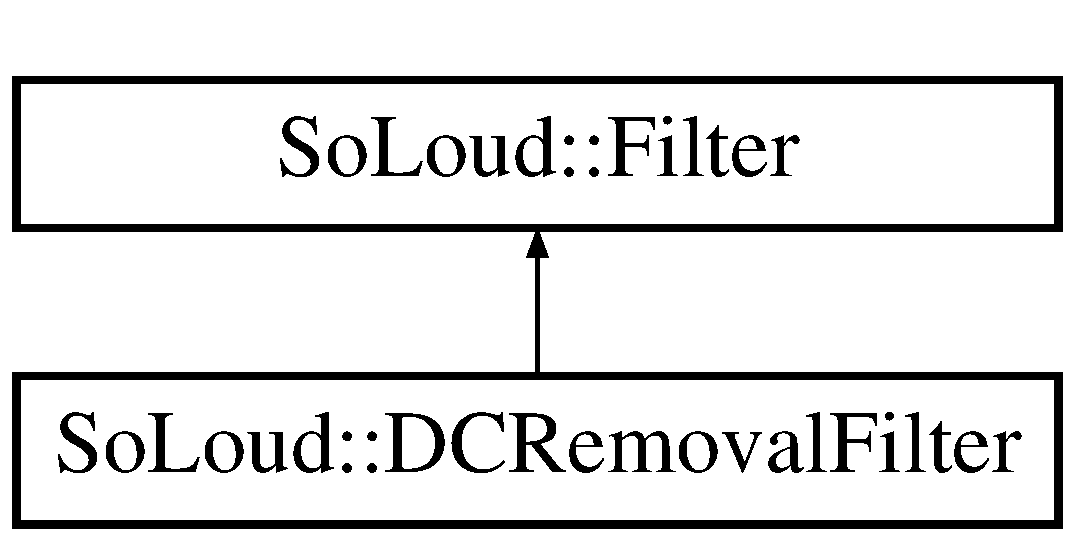
\includegraphics[height=2.000000cm]{class_so_loud_1_1_d_c_removal_filter}
\end{center}
\end{figure}
\subsection*{Public Member Functions}
\begin{DoxyCompactItemize}
\item 
\mbox{\Hypertarget{class_so_loud_1_1_d_c_removal_filter_a59917116078dd4e42cff7185f563597e}\label{class_so_loud_1_1_d_c_removal_filter_a59917116078dd4e42cff7185f563597e}} 
virtual \mbox{\hyperlink{class_so_loud_1_1_filter_instance}{Filter\+Instance}} $\ast$ {\bfseries create\+Instance} ()
\item 
\mbox{\Hypertarget{class_so_loud_1_1_d_c_removal_filter_aace2e51a78bd1457b719d67079bb1bcd}\label{class_so_loud_1_1_d_c_removal_filter_aace2e51a78bd1457b719d67079bb1bcd}} 
result {\bfseries set\+Params} (float a\+Length=0.\+1f)
\end{DoxyCompactItemize}
\subsection*{Public Attributes}
\begin{DoxyCompactItemize}
\item 
\mbox{\Hypertarget{class_so_loud_1_1_d_c_removal_filter_ac2f6517e56840935aade3cfcce7bfcec}\label{class_so_loud_1_1_d_c_removal_filter_ac2f6517e56840935aade3cfcce7bfcec}} 
float {\bfseries m\+Length}
\end{DoxyCompactItemize}


The documentation for this class was generated from the following file\+:\begin{DoxyCompactItemize}
\item 
deps/\+E\+S\+A\+T/include/\+E\+S\+A\+T\+\_\+extra/soloud/soloud\+\_\+dcremovalfilter.\+h\end{DoxyCompactItemize}

\hypertarget{class_so_loud_1_1_d_c_removal_filter_instance}{}\section{So\+Loud\+:\+:D\+C\+Removal\+Filter\+Instance Class Reference}
\label{class_so_loud_1_1_d_c_removal_filter_instance}\index{So\+Loud\+::\+D\+C\+Removal\+Filter\+Instance@{So\+Loud\+::\+D\+C\+Removal\+Filter\+Instance}}
Inheritance diagram for So\+Loud\+:\+:D\+C\+Removal\+Filter\+Instance\+:\begin{figure}[H]
\begin{center}
\leavevmode
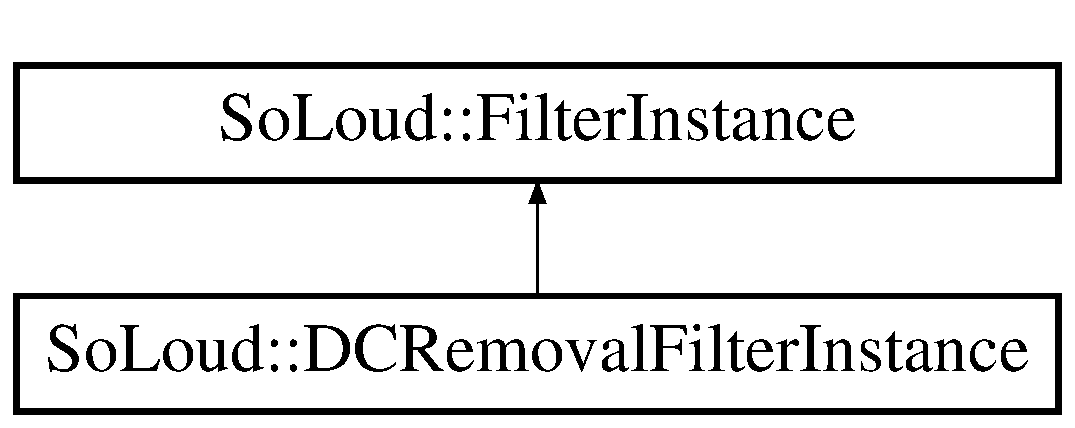
\includegraphics[height=2.000000cm]{class_so_loud_1_1_d_c_removal_filter_instance}
\end{center}
\end{figure}
\subsection*{Public Member Functions}
\begin{DoxyCompactItemize}
\item 
\mbox{\Hypertarget{class_so_loud_1_1_d_c_removal_filter_instance_aa421cd674e792ea9989de1f0c4e12409}\label{class_so_loud_1_1_d_c_removal_filter_instance_aa421cd674e792ea9989de1f0c4e12409}} 
virtual void {\bfseries filter} (float $\ast$a\+Buffer, unsigned int a\+Samples, unsigned int a\+Channels, float a\+Samplerate, time a\+Time)
\item 
\mbox{\Hypertarget{class_so_loud_1_1_d_c_removal_filter_instance_a761eab639e22ec88ae747a58795a9337}\label{class_so_loud_1_1_d_c_removal_filter_instance_a761eab639e22ec88ae747a58795a9337}} 
{\bfseries D\+C\+Removal\+Filter\+Instance} (\mbox{\hyperlink{class_so_loud_1_1_d_c_removal_filter}{D\+C\+Removal\+Filter}} $\ast$a\+Parent)
\end{DoxyCompactItemize}
\subsection*{Additional Inherited Members}


The documentation for this class was generated from the following file\+:\begin{DoxyCompactItemize}
\item 
deps/\+E\+S\+A\+T/include/\+E\+S\+A\+T\+\_\+extra/soloud/soloud\+\_\+dcremovalfilter.\+h\end{DoxyCompactItemize}

\hypertarget{class_so_loud_1_1_disk_file}{}\section{So\+Loud\+:\+:Disk\+File Class Reference}
\label{class_so_loud_1_1_disk_file}\index{So\+Loud\+::\+Disk\+File@{So\+Loud\+::\+Disk\+File}}
Inheritance diagram for So\+Loud\+:\+:Disk\+File\+:\begin{figure}[H]
\begin{center}
\leavevmode
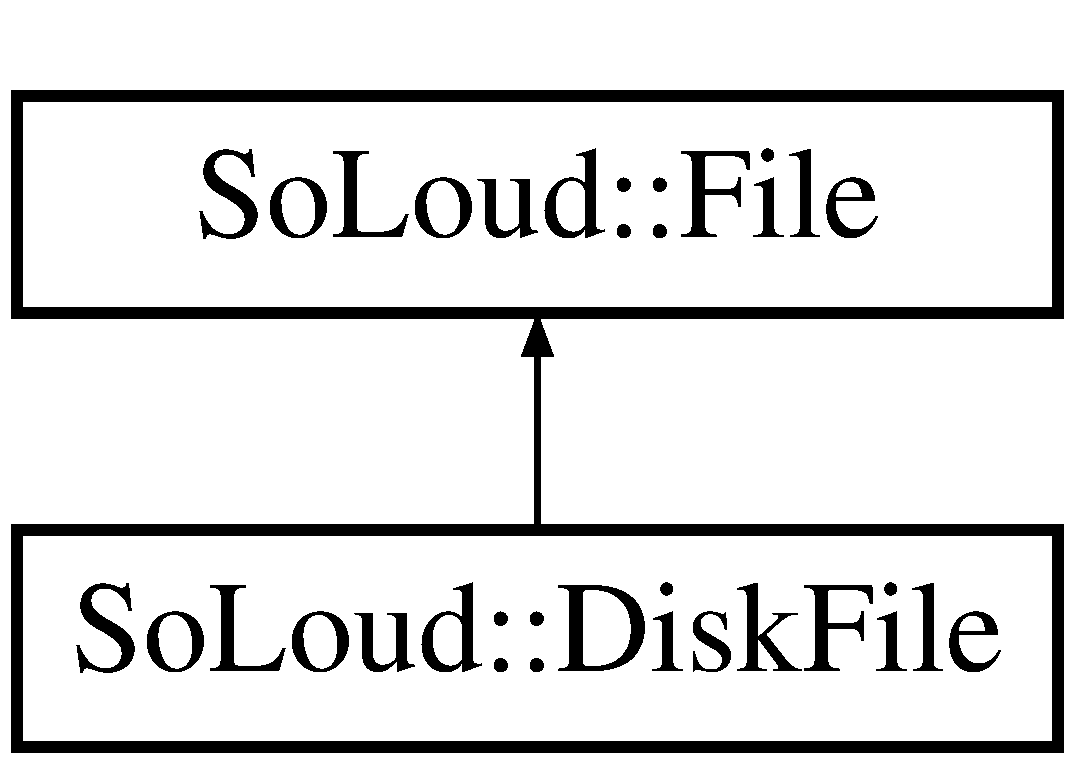
\includegraphics[height=2.000000cm]{class_so_loud_1_1_disk_file}
\end{center}
\end{figure}
\subsection*{Public Member Functions}
\begin{DoxyCompactItemize}
\item 
\mbox{\Hypertarget{class_so_loud_1_1_disk_file_ab865962be3faa73abd7df013961059bb}\label{class_so_loud_1_1_disk_file_ab865962be3faa73abd7df013961059bb}} 
virtual int {\bfseries eof} ()
\item 
\mbox{\Hypertarget{class_so_loud_1_1_disk_file_a8c0f8b5adf303cf51ccd793a02348a7c}\label{class_so_loud_1_1_disk_file_a8c0f8b5adf303cf51ccd793a02348a7c}} 
virtual unsigned int {\bfseries read} (unsigned char $\ast$a\+Dst, unsigned int a\+Bytes)
\item 
\mbox{\Hypertarget{class_so_loud_1_1_disk_file_ad6ba18b0d37b2245f0cc59b6077f7fcd}\label{class_so_loud_1_1_disk_file_ad6ba18b0d37b2245f0cc59b6077f7fcd}} 
virtual unsigned int {\bfseries length} ()
\item 
\mbox{\Hypertarget{class_so_loud_1_1_disk_file_a7e0c8ee42fd0a39ea999819d77fcc036}\label{class_so_loud_1_1_disk_file_a7e0c8ee42fd0a39ea999819d77fcc036}} 
virtual void {\bfseries seek} (int a\+Offset)
\item 
\mbox{\Hypertarget{class_so_loud_1_1_disk_file_a1a404b8aded2cccbd4bc2332b2e9f1b5}\label{class_so_loud_1_1_disk_file_a1a404b8aded2cccbd4bc2332b2e9f1b5}} 
virtual unsigned int {\bfseries pos} ()
\item 
\mbox{\Hypertarget{class_so_loud_1_1_disk_file_ae9f3fc6d8b13f91fa1d9f4136a4643a4}\label{class_so_loud_1_1_disk_file_ae9f3fc6d8b13f91fa1d9f4136a4643a4}} 
result {\bfseries open} (const char $\ast$a\+Filename)
\item 
\mbox{\Hypertarget{class_so_loud_1_1_disk_file_a2a350a2d9326e39bb0b77b809aa69128}\label{class_so_loud_1_1_disk_file_a2a350a2d9326e39bb0b77b809aa69128}} 
virtual F\+I\+LE $\ast$ {\bfseries get\+File\+Ptr} ()
\end{DoxyCompactItemize}
\subsection*{Public Attributes}
\begin{DoxyCompactItemize}
\item 
\mbox{\Hypertarget{class_so_loud_1_1_disk_file_a310c115f8d717792fc5c242095dc532d}\label{class_so_loud_1_1_disk_file_a310c115f8d717792fc5c242095dc532d}} 
F\+I\+LE $\ast$ {\bfseries m\+File\+Handle}
\end{DoxyCompactItemize}


The documentation for this class was generated from the following file\+:\begin{DoxyCompactItemize}
\item 
deps/\+E\+S\+A\+T/include/\+E\+S\+A\+T\+\_\+extra/soloud/soloud\+\_\+file.\+h\end{DoxyCompactItemize}

\hypertarget{class_so_loud_1_1_echo_filter}{}\section{So\+Loud\+:\+:Echo\+Filter Class Reference}
\label{class_so_loud_1_1_echo_filter}\index{So\+Loud\+::\+Echo\+Filter@{So\+Loud\+::\+Echo\+Filter}}
Inheritance diagram for So\+Loud\+:\+:Echo\+Filter\+:\begin{figure}[H]
\begin{center}
\leavevmode
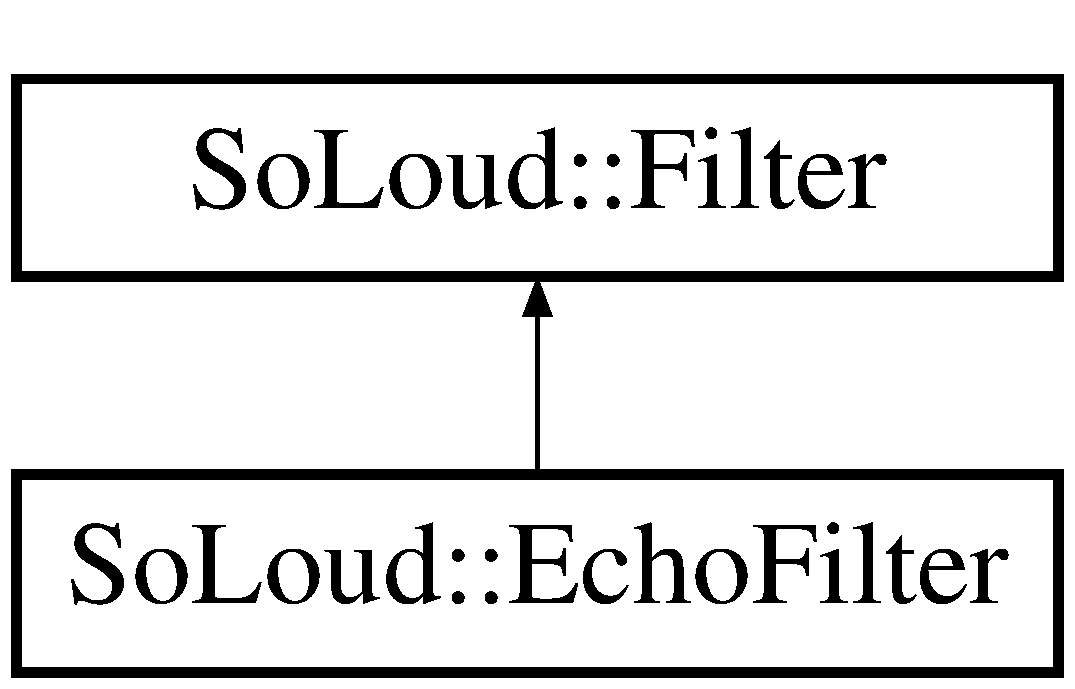
\includegraphics[height=2.000000cm]{class_so_loud_1_1_echo_filter}
\end{center}
\end{figure}
\subsection*{Public Member Functions}
\begin{DoxyCompactItemize}
\item 
\mbox{\Hypertarget{class_so_loud_1_1_echo_filter_a52bef9ece5674bbf2c8391fd8ef03d06}\label{class_so_loud_1_1_echo_filter_a52bef9ece5674bbf2c8391fd8ef03d06}} 
virtual \mbox{\hyperlink{class_so_loud_1_1_filter_instance}{Filter\+Instance}} $\ast$ {\bfseries create\+Instance} ()
\item 
\mbox{\Hypertarget{class_so_loud_1_1_echo_filter_adf9a75c94ca8451d7ab599e4cd9387bd}\label{class_so_loud_1_1_echo_filter_adf9a75c94ca8451d7ab599e4cd9387bd}} 
result {\bfseries set\+Params} (float a\+Delay, float a\+Decay=0.\+7f, float a\+Filter=0.\+0f)
\end{DoxyCompactItemize}
\subsection*{Public Attributes}
\begin{DoxyCompactItemize}
\item 
\mbox{\Hypertarget{class_so_loud_1_1_echo_filter_a14a5bdf6c0bb264dc4fb517961fc8e13}\label{class_so_loud_1_1_echo_filter_a14a5bdf6c0bb264dc4fb517961fc8e13}} 
float {\bfseries m\+Delay}
\item 
\mbox{\Hypertarget{class_so_loud_1_1_echo_filter_a1e11873461a6393defa8ed04cea81a69}\label{class_so_loud_1_1_echo_filter_a1e11873461a6393defa8ed04cea81a69}} 
float {\bfseries m\+Decay}
\item 
\mbox{\Hypertarget{class_so_loud_1_1_echo_filter_ab7fa97fec38e74941837b6ed0853e3c3}\label{class_so_loud_1_1_echo_filter_ab7fa97fec38e74941837b6ed0853e3c3}} 
float {\bfseries m\+Filter}
\end{DoxyCompactItemize}


The documentation for this class was generated from the following file\+:\begin{DoxyCompactItemize}
\item 
deps/\+E\+S\+A\+T/include/\+E\+S\+A\+T\+\_\+extra/soloud/soloud\+\_\+echofilter.\+h\end{DoxyCompactItemize}

\hypertarget{class_so_loud_1_1_echo_filter_instance}{}\section{So\+Loud\+:\+:Echo\+Filter\+Instance Class Reference}
\label{class_so_loud_1_1_echo_filter_instance}\index{So\+Loud\+::\+Echo\+Filter\+Instance@{So\+Loud\+::\+Echo\+Filter\+Instance}}
Inheritance diagram for So\+Loud\+:\+:Echo\+Filter\+Instance\+:\begin{figure}[H]
\begin{center}
\leavevmode
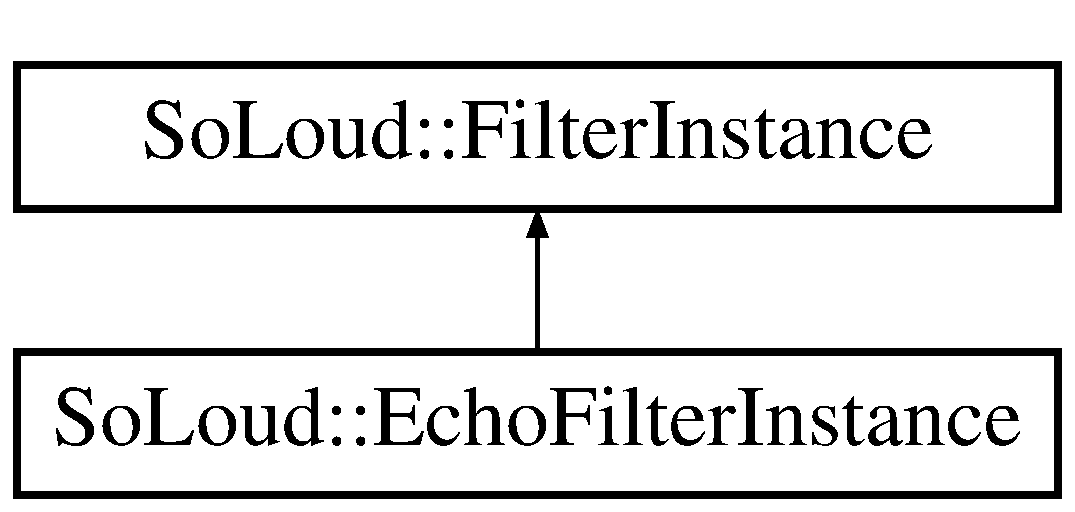
\includegraphics[height=2.000000cm]{class_so_loud_1_1_echo_filter_instance}
\end{center}
\end{figure}
\subsection*{Public Member Functions}
\begin{DoxyCompactItemize}
\item 
\mbox{\Hypertarget{class_so_loud_1_1_echo_filter_instance_a70347a6f9b0ec23b06ebf6da94b63259}\label{class_so_loud_1_1_echo_filter_instance_a70347a6f9b0ec23b06ebf6da94b63259}} 
virtual void {\bfseries filter} (float $\ast$a\+Buffer, unsigned int a\+Samples, unsigned int a\+Channels, float a\+Samplerate, time a\+Time)
\item 
\mbox{\Hypertarget{class_so_loud_1_1_echo_filter_instance_ab2584f4cbaa08c31555538a7a557ee70}\label{class_so_loud_1_1_echo_filter_instance_ab2584f4cbaa08c31555538a7a557ee70}} 
{\bfseries Echo\+Filter\+Instance} (\mbox{\hyperlink{class_so_loud_1_1_echo_filter}{Echo\+Filter}} $\ast$a\+Parent)
\end{DoxyCompactItemize}
\subsection*{Additional Inherited Members}


The documentation for this class was generated from the following file\+:\begin{DoxyCompactItemize}
\item 
deps/\+E\+S\+A\+T/include/\+E\+S\+A\+T\+\_\+extra/soloud/soloud\+\_\+echofilter.\+h\end{DoxyCompactItemize}

\hypertarget{class_so_loud_1_1_fader}{}\section{So\+Loud\+:\+:Fader Class Reference}
\label{class_so_loud_1_1_fader}\index{So\+Loud\+::\+Fader@{So\+Loud\+::\+Fader}}
\subsection*{Public Member Functions}
\begin{DoxyCompactItemize}
\item 
\mbox{\Hypertarget{class_so_loud_1_1_fader_ab832eabb3306ab0b51a6085f50dfe15c}\label{class_so_loud_1_1_fader_ab832eabb3306ab0b51a6085f50dfe15c}} 
void {\bfseries set\+L\+FO} (float a\+From, float a\+To, time a\+Time, time a\+Start\+Time)
\item 
\mbox{\Hypertarget{class_so_loud_1_1_fader_a75bbcceb1df1300da93bb198076a818b}\label{class_so_loud_1_1_fader_a75bbcceb1df1300da93bb198076a818b}} 
void {\bfseries set} (float a\+From, float a\+To, time a\+Time, time a\+Start\+Time)
\item 
\mbox{\Hypertarget{class_so_loud_1_1_fader_a7a6639fa22a5d7e10f04a473e65eeba1}\label{class_so_loud_1_1_fader_a7a6639fa22a5d7e10f04a473e65eeba1}} 
float {\bfseries get} (time a\+Current\+Time)
\end{DoxyCompactItemize}
\subsection*{Public Attributes}
\begin{DoxyCompactItemize}
\item 
\mbox{\Hypertarget{class_so_loud_1_1_fader_a96a14cb384b0b5a6da2f822aeb771f66}\label{class_so_loud_1_1_fader_a96a14cb384b0b5a6da2f822aeb771f66}} 
float {\bfseries m\+From}
\item 
\mbox{\Hypertarget{class_so_loud_1_1_fader_ab83ca38acdf6a04538c041c9c1fd7f13}\label{class_so_loud_1_1_fader_ab83ca38acdf6a04538c041c9c1fd7f13}} 
float {\bfseries m\+To}
\item 
\mbox{\Hypertarget{class_so_loud_1_1_fader_a99ec0e7cf010c0e3e86998841cfea7e5}\label{class_so_loud_1_1_fader_a99ec0e7cf010c0e3e86998841cfea7e5}} 
float {\bfseries m\+Delta}
\item 
\mbox{\Hypertarget{class_so_loud_1_1_fader_a6bc8f56f9bd609a34438e427fff7a22f}\label{class_so_loud_1_1_fader_a6bc8f56f9bd609a34438e427fff7a22f}} 
time {\bfseries m\+Time}
\item 
\mbox{\Hypertarget{class_so_loud_1_1_fader_a56ce1ecbabe751f09263e56254790f2b}\label{class_so_loud_1_1_fader_a56ce1ecbabe751f09263e56254790f2b}} 
time {\bfseries m\+Start\+Time}
\item 
\mbox{\Hypertarget{class_so_loud_1_1_fader_a5e0de582ca2a1c8feadad998d6dd58e0}\label{class_so_loud_1_1_fader_a5e0de582ca2a1c8feadad998d6dd58e0}} 
time {\bfseries m\+End\+Time}
\item 
\mbox{\Hypertarget{class_so_loud_1_1_fader_a6cc1d2a5d4e0f411e1742d4586a663fe}\label{class_so_loud_1_1_fader_a6cc1d2a5d4e0f411e1742d4586a663fe}} 
float {\bfseries m\+Current}
\item 
\mbox{\Hypertarget{class_so_loud_1_1_fader_aebf85d7751bb64982fdc3045798315a4}\label{class_so_loud_1_1_fader_aebf85d7751bb64982fdc3045798315a4}} 
int {\bfseries m\+Active}
\end{DoxyCompactItemize}


The documentation for this class was generated from the following file\+:\begin{DoxyCompactItemize}
\item 
deps/\+E\+S\+A\+T/include/\+E\+S\+A\+T\+\_\+extra/soloud/soloud\+\_\+fader.\+h\end{DoxyCompactItemize}

\hypertarget{class_so_loud_1_1_f_f_t_filter}{}\section{So\+Loud\+:\+:F\+F\+T\+Filter Class Reference}
\label{class_so_loud_1_1_f_f_t_filter}\index{So\+Loud\+::\+F\+F\+T\+Filter@{So\+Loud\+::\+F\+F\+T\+Filter}}
Inheritance diagram for So\+Loud\+:\+:F\+F\+T\+Filter\+:\begin{figure}[H]
\begin{center}
\leavevmode
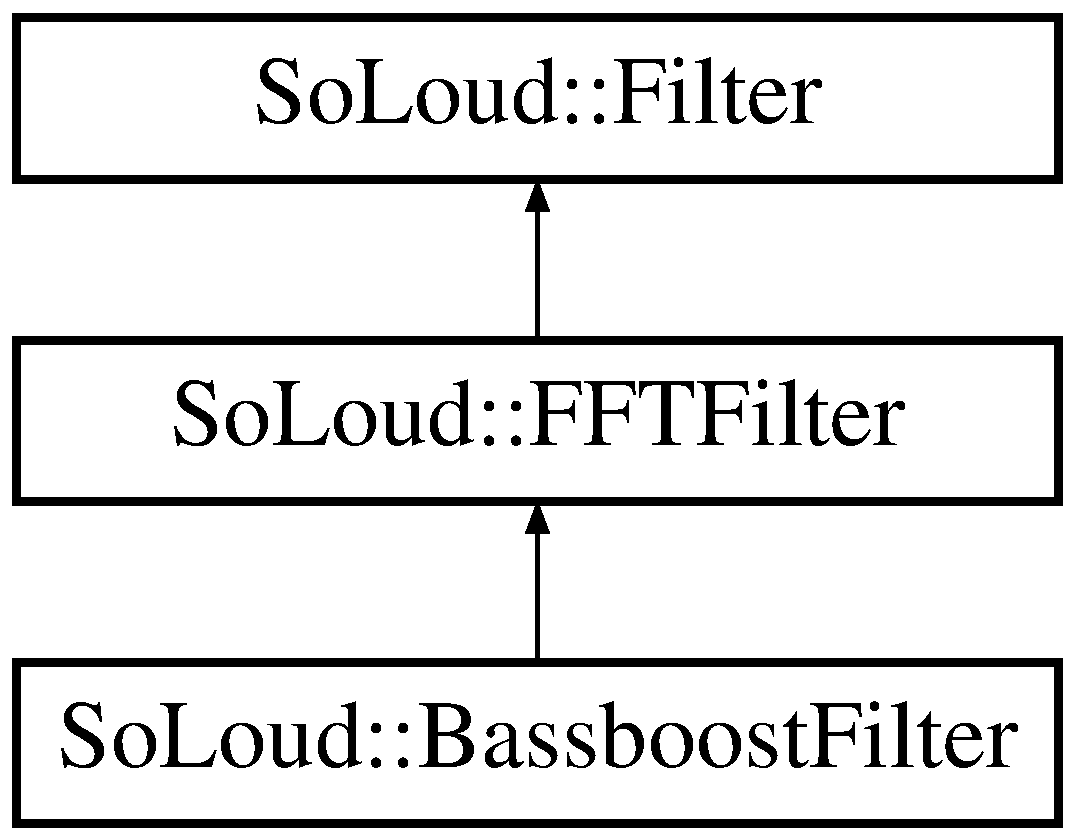
\includegraphics[height=3.000000cm]{class_so_loud_1_1_f_f_t_filter}
\end{center}
\end{figure}
\subsection*{Public Member Functions}
\begin{DoxyCompactItemize}
\item 
\mbox{\Hypertarget{class_so_loud_1_1_f_f_t_filter_a4a0ca82f6ad367aab4eb8baa09e6bb2e}\label{class_so_loud_1_1_f_f_t_filter_a4a0ca82f6ad367aab4eb8baa09e6bb2e}} 
virtual \mbox{\hyperlink{class_so_loud_1_1_filter_instance}{Filter\+Instance}} $\ast$ {\bfseries create\+Instance} ()
\end{DoxyCompactItemize}


The documentation for this class was generated from the following file\+:\begin{DoxyCompactItemize}
\item 
deps/\+E\+S\+A\+T/include/\+E\+S\+A\+T\+\_\+extra/soloud/soloud\+\_\+fftfilter.\+h\end{DoxyCompactItemize}

\hypertarget{class_so_loud_1_1_f_f_t_filter_instance}{}\section{So\+Loud\+:\+:F\+F\+T\+Filter\+Instance Class Reference}
\label{class_so_loud_1_1_f_f_t_filter_instance}\index{So\+Loud\+::\+F\+F\+T\+Filter\+Instance@{So\+Loud\+::\+F\+F\+T\+Filter\+Instance}}
Inheritance diagram for So\+Loud\+:\+:F\+F\+T\+Filter\+Instance\+:\begin{figure}[H]
\begin{center}
\leavevmode
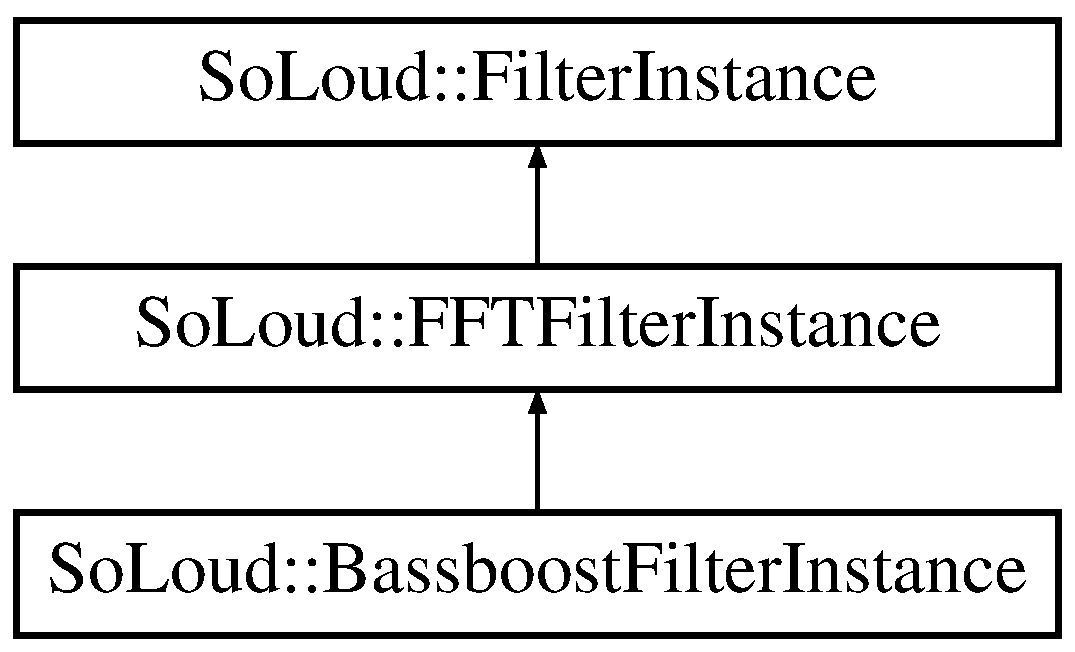
\includegraphics[height=3.000000cm]{class_so_loud_1_1_f_f_t_filter_instance}
\end{center}
\end{figure}
\subsection*{Public Member Functions}
\begin{DoxyCompactItemize}
\item 
\mbox{\Hypertarget{class_so_loud_1_1_f_f_t_filter_instance_a6968362e2c8d2ff62064b3f3c010de75}\label{class_so_loud_1_1_f_f_t_filter_instance_a6968362e2c8d2ff62064b3f3c010de75}} 
virtual void {\bfseries fft\+Filter\+Channel} (float $\ast$a\+F\+F\+T\+Buffer, unsigned int a\+Samples, float a\+Samplerate, time a\+Time, unsigned int a\+Channel, unsigned int a\+Channels)
\item 
\mbox{\Hypertarget{class_so_loud_1_1_f_f_t_filter_instance_ac110bb616aa490437b4b5b97a8ffd6f8}\label{class_so_loud_1_1_f_f_t_filter_instance_ac110bb616aa490437b4b5b97a8ffd6f8}} 
virtual void {\bfseries filter\+Channel} (float $\ast$a\+Buffer, unsigned int a\+Samples, float a\+Samplerate, time a\+Time, unsigned int a\+Channel, unsigned int a\+Channels)
\item 
\mbox{\Hypertarget{class_so_loud_1_1_f_f_t_filter_instance_a00e5d27d93741b35910581ef36c003fa}\label{class_so_loud_1_1_f_f_t_filter_instance_a00e5d27d93741b35910581ef36c003fa}} 
{\bfseries F\+F\+T\+Filter\+Instance} (\mbox{\hyperlink{class_so_loud_1_1_f_f_t_filter}{F\+F\+T\+Filter}} $\ast$a\+Parent)
\end{DoxyCompactItemize}
\subsection*{Additional Inherited Members}


The documentation for this class was generated from the following file\+:\begin{DoxyCompactItemize}
\item 
deps/\+E\+S\+A\+T/include/\+E\+S\+A\+T\+\_\+extra/soloud/soloud\+\_\+fftfilter.\+h\end{DoxyCompactItemize}

\hypertarget{class_so_loud_1_1_file}{}\section{So\+Loud\+:\+:File Class Reference}
\label{class_so_loud_1_1_file}\index{So\+Loud\+::\+File@{So\+Loud\+::\+File}}
Inheritance diagram for So\+Loud\+:\+:File\+:\begin{figure}[H]
\begin{center}
\leavevmode
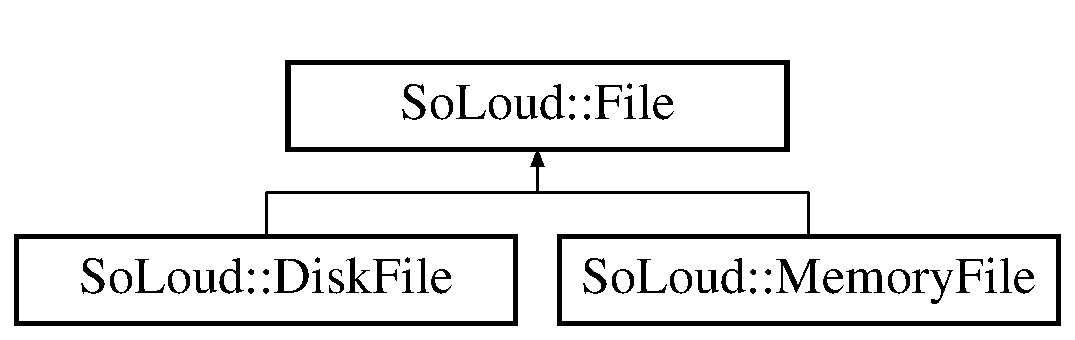
\includegraphics[height=2.000000cm]{class_so_loud_1_1_file}
\end{center}
\end{figure}
\subsection*{Public Member Functions}
\begin{DoxyCompactItemize}
\item 
\mbox{\Hypertarget{class_so_loud_1_1_file_a2b811550ddbfea1e1f33af18f26e15db}\label{class_so_loud_1_1_file_a2b811550ddbfea1e1f33af18f26e15db}} 
unsigned int {\bfseries read8} ()
\item 
\mbox{\Hypertarget{class_so_loud_1_1_file_afc03885cd3810bf6be24140be8907078}\label{class_so_loud_1_1_file_afc03885cd3810bf6be24140be8907078}} 
unsigned int {\bfseries read16} ()
\item 
\mbox{\Hypertarget{class_so_loud_1_1_file_a12225d0232f062979aca7ba02f6cd5c3}\label{class_so_loud_1_1_file_a12225d0232f062979aca7ba02f6cd5c3}} 
unsigned int {\bfseries read32} ()
\item 
\mbox{\Hypertarget{class_so_loud_1_1_file_ad396b449fdfc04b2a5def8d1ccf98b17}\label{class_so_loud_1_1_file_ad396b449fdfc04b2a5def8d1ccf98b17}} 
virtual int {\bfseries eof} ()=0
\item 
\mbox{\Hypertarget{class_so_loud_1_1_file_ad4c53f330a32d0af3d5e90d0add22274}\label{class_so_loud_1_1_file_ad4c53f330a32d0af3d5e90d0add22274}} 
virtual unsigned int {\bfseries read} (unsigned char $\ast$a\+Dst, unsigned int a\+Bytes)=0
\item 
\mbox{\Hypertarget{class_so_loud_1_1_file_aa25300482995ab849ca6e0115b9bd7bf}\label{class_so_loud_1_1_file_aa25300482995ab849ca6e0115b9bd7bf}} 
virtual unsigned int {\bfseries length} ()=0
\item 
\mbox{\Hypertarget{class_so_loud_1_1_file_a28078d314c7b390edd82469f7e4d75a4}\label{class_so_loud_1_1_file_a28078d314c7b390edd82469f7e4d75a4}} 
virtual void {\bfseries seek} (int a\+Offset)=0
\item 
\mbox{\Hypertarget{class_so_loud_1_1_file_a619881eac4b1c7e0867d0924970bf916}\label{class_so_loud_1_1_file_a619881eac4b1c7e0867d0924970bf916}} 
virtual unsigned int {\bfseries pos} ()=0
\item 
\mbox{\Hypertarget{class_so_loud_1_1_file_a137ccbea0200f10f0e6f3c1314e5e0a6}\label{class_so_loud_1_1_file_a137ccbea0200f10f0e6f3c1314e5e0a6}} 
virtual F\+I\+LE $\ast$ {\bfseries get\+File\+Ptr} ()
\item 
\mbox{\Hypertarget{class_so_loud_1_1_file_a620728769391db660d290c0433624683}\label{class_so_loud_1_1_file_a620728769391db660d290c0433624683}} 
virtual unsigned char $\ast$ {\bfseries get\+Mem\+Ptr} ()
\end{DoxyCompactItemize}


The documentation for this class was generated from the following file\+:\begin{DoxyCompactItemize}
\item 
deps/\+E\+S\+A\+T/include/\+E\+S\+A\+T\+\_\+extra/soloud/soloud\+\_\+file.\+h\end{DoxyCompactItemize}

\hypertarget{class_so_loud_1_1_filter}{}\section{So\+Loud\+:\+:Filter Class Reference}
\label{class_so_loud_1_1_filter}\index{So\+Loud\+::\+Filter@{So\+Loud\+::\+Filter}}
Inheritance diagram for So\+Loud\+:\+:Filter\+:\begin{figure}[H]
\begin{center}
\leavevmode
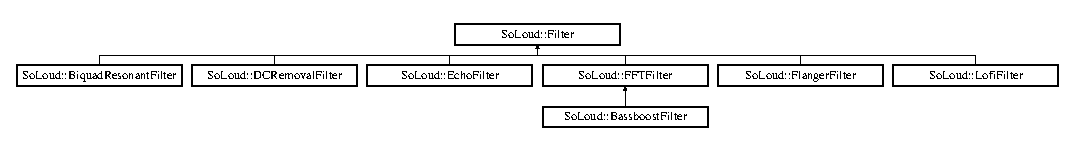
\includegraphics[height=1.489362cm]{class_so_loud_1_1_filter}
\end{center}
\end{figure}
\subsection*{Public Member Functions}
\begin{DoxyCompactItemize}
\item 
\mbox{\Hypertarget{class_so_loud_1_1_filter_ad1a2997835abacc79f5780dd42830583}\label{class_so_loud_1_1_filter_ad1a2997835abacc79f5780dd42830583}} 
virtual \mbox{\hyperlink{class_so_loud_1_1_filter_instance}{Filter\+Instance}} $\ast$ {\bfseries create\+Instance} ()=0
\end{DoxyCompactItemize}


The documentation for this class was generated from the following file\+:\begin{DoxyCompactItemize}
\item 
deps/\+E\+S\+A\+T/include/\+E\+S\+A\+T\+\_\+extra/soloud/soloud\+\_\+filter.\+h\end{DoxyCompactItemize}

\hypertarget{class_so_loud_1_1_filter_instance}{}\section{So\+Loud\+:\+:Filter\+Instance Class Reference}
\label{class_so_loud_1_1_filter_instance}\index{So\+Loud\+::\+Filter\+Instance@{So\+Loud\+::\+Filter\+Instance}}
Inheritance diagram for So\+Loud\+:\+:Filter\+Instance\+:\begin{figure}[H]
\begin{center}
\leavevmode
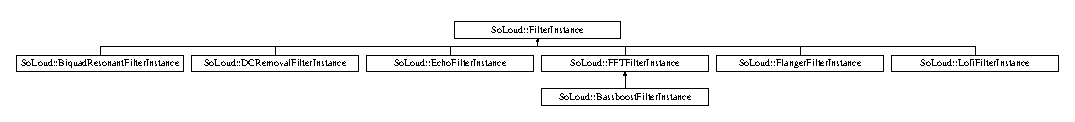
\includegraphics[height=1.191489cm]{class_so_loud_1_1_filter_instance}
\end{center}
\end{figure}
\subsection*{Public Member Functions}
\begin{DoxyCompactItemize}
\item 
\mbox{\Hypertarget{class_so_loud_1_1_filter_instance_a3546d0b3c87e4a44cea482fa3c1ce2ef}\label{class_so_loud_1_1_filter_instance_a3546d0b3c87e4a44cea482fa3c1ce2ef}} 
virtual result {\bfseries init\+Params} (int a\+Num\+Params)
\item 
\mbox{\Hypertarget{class_so_loud_1_1_filter_instance_ac2b293594bd3aed7bc70bb1fe1e8da95}\label{class_so_loud_1_1_filter_instance_ac2b293594bd3aed7bc70bb1fe1e8da95}} 
virtual void {\bfseries update\+Params} (time a\+Time)
\item 
\mbox{\Hypertarget{class_so_loud_1_1_filter_instance_a65d38ac0562733c195898018b6c3ff47}\label{class_so_loud_1_1_filter_instance_a65d38ac0562733c195898018b6c3ff47}} 
virtual void {\bfseries filter} (float $\ast$a\+Buffer, unsigned int a\+Samples, unsigned int a\+Channels, float a\+Samplerate, time a\+Time)
\item 
\mbox{\Hypertarget{class_so_loud_1_1_filter_instance_aa4ad1fcd3c9f37262cbdf4467109a12f}\label{class_so_loud_1_1_filter_instance_aa4ad1fcd3c9f37262cbdf4467109a12f}} 
virtual void {\bfseries filter\+Channel} (float $\ast$a\+Buffer, unsigned int a\+Samples, float a\+Samplerate, time a\+Time, unsigned int a\+Channel, unsigned int a\+Channels)
\item 
\mbox{\Hypertarget{class_so_loud_1_1_filter_instance_a8d709cb743fc9a80eed830adafa399a4}\label{class_so_loud_1_1_filter_instance_a8d709cb743fc9a80eed830adafa399a4}} 
virtual float {\bfseries get\+Filter\+Parameter} (unsigned int a\+Attribute\+Id)
\item 
\mbox{\Hypertarget{class_so_loud_1_1_filter_instance_aa4ee94f287006e35a0f1582ff471a62a}\label{class_so_loud_1_1_filter_instance_aa4ee94f287006e35a0f1582ff471a62a}} 
virtual void {\bfseries set\+Filter\+Parameter} (unsigned int a\+Attribute\+Id, float a\+Value)
\item 
\mbox{\Hypertarget{class_so_loud_1_1_filter_instance_a9a3f9f37aac5e782e2f3c1260bdc15f4}\label{class_so_loud_1_1_filter_instance_a9a3f9f37aac5e782e2f3c1260bdc15f4}} 
virtual void {\bfseries fade\+Filter\+Parameter} (unsigned int a\+Attribute\+Id, float a\+To, time a\+Time, time a\+Start\+Time)
\item 
\mbox{\Hypertarget{class_so_loud_1_1_filter_instance_a219b1fb211b5599bf70f0d6403522978}\label{class_so_loud_1_1_filter_instance_a219b1fb211b5599bf70f0d6403522978}} 
virtual void {\bfseries oscillate\+Filter\+Parameter} (unsigned int a\+Attribute\+Id, float a\+From, float a\+To, time a\+Time, time a\+Start\+Time)
\end{DoxyCompactItemize}
\subsection*{Public Attributes}
\begin{DoxyCompactItemize}
\item 
\mbox{\Hypertarget{class_so_loud_1_1_filter_instance_a3543039db3c00cd19b7d01b82c29d824}\label{class_so_loud_1_1_filter_instance_a3543039db3c00cd19b7d01b82c29d824}} 
unsigned int {\bfseries m\+Num\+Params}
\item 
\mbox{\Hypertarget{class_so_loud_1_1_filter_instance_a4ed9e55584ed2ae59e3de878dfa8c506}\label{class_so_loud_1_1_filter_instance_a4ed9e55584ed2ae59e3de878dfa8c506}} 
unsigned int {\bfseries m\+Param\+Changed}
\item 
\mbox{\Hypertarget{class_so_loud_1_1_filter_instance_ab60599cfa1fcdf09e1a5753399e04048}\label{class_so_loud_1_1_filter_instance_ab60599cfa1fcdf09e1a5753399e04048}} 
float $\ast$ {\bfseries m\+Param}
\item 
\mbox{\Hypertarget{class_so_loud_1_1_filter_instance_ab30e49b98d87f106fc1202793120cac7}\label{class_so_loud_1_1_filter_instance_ab30e49b98d87f106fc1202793120cac7}} 
\mbox{\hyperlink{class_so_loud_1_1_fader}{Fader}} $\ast$ {\bfseries m\+Param\+Fader}
\end{DoxyCompactItemize}


The documentation for this class was generated from the following file\+:\begin{DoxyCompactItemize}
\item 
deps/\+E\+S\+A\+T/include/\+E\+S\+A\+T\+\_\+extra/soloud/soloud\+\_\+filter.\+h\end{DoxyCompactItemize}

\hypertarget{class_so_loud_1_1_flanger_filter}{}\section{So\+Loud\+:\+:Flanger\+Filter Class Reference}
\label{class_so_loud_1_1_flanger_filter}\index{So\+Loud\+::\+Flanger\+Filter@{So\+Loud\+::\+Flanger\+Filter}}
Inheritance diagram for So\+Loud\+:\+:Flanger\+Filter\+:\begin{figure}[H]
\begin{center}
\leavevmode
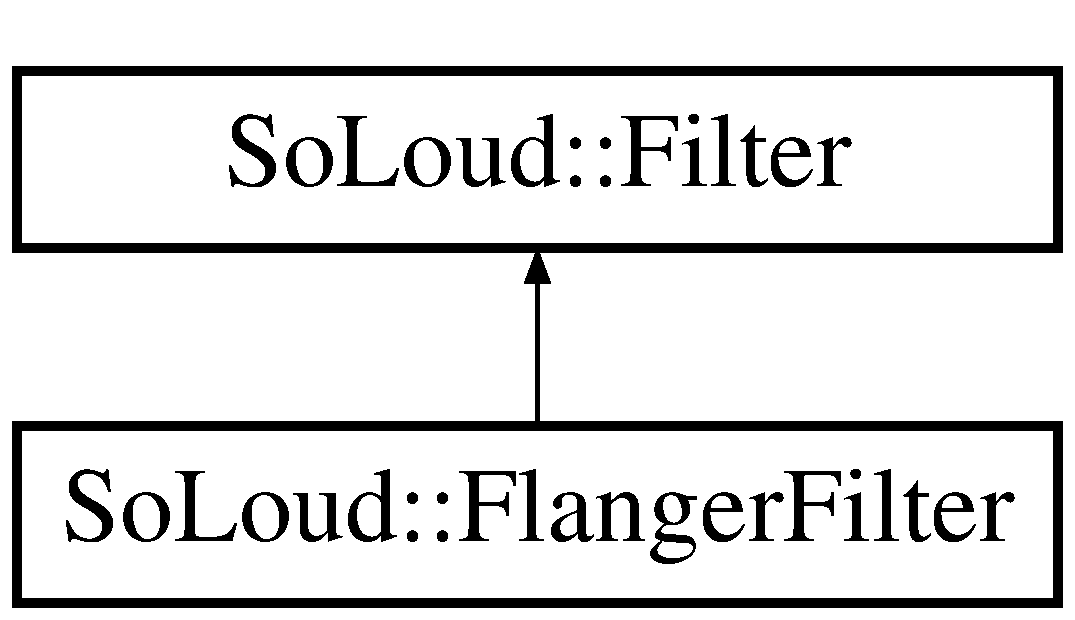
\includegraphics[height=2.000000cm]{class_so_loud_1_1_flanger_filter}
\end{center}
\end{figure}
\subsection*{Public Types}
\begin{DoxyCompactItemize}
\item 
\mbox{\Hypertarget{class_so_loud_1_1_flanger_filter_a0016bc09925e106d4de01686892a8eb7}\label{class_so_loud_1_1_flanger_filter_a0016bc09925e106d4de01686892a8eb7}} 
enum {\bfseries F\+I\+L\+T\+E\+R\+P\+A\+R\+A\+MS} \{ {\bfseries W\+ET}, 
{\bfseries D\+E\+L\+AY}, 
{\bfseries F\+R\+EQ}
 \}
\end{DoxyCompactItemize}
\subsection*{Public Member Functions}
\begin{DoxyCompactItemize}
\item 
\mbox{\Hypertarget{class_so_loud_1_1_flanger_filter_a7abf8a3b961902b84d7b634826c83a10}\label{class_so_loud_1_1_flanger_filter_a7abf8a3b961902b84d7b634826c83a10}} 
virtual \mbox{\hyperlink{class_so_loud_1_1_filter_instance}{Filter\+Instance}} $\ast$ {\bfseries create\+Instance} ()
\item 
\mbox{\Hypertarget{class_so_loud_1_1_flanger_filter_aa483de45fd8458b9365b9012e83c0bd3}\label{class_so_loud_1_1_flanger_filter_aa483de45fd8458b9365b9012e83c0bd3}} 
result {\bfseries set\+Params} (float a\+Delay, float a\+Freq)
\end{DoxyCompactItemize}
\subsection*{Public Attributes}
\begin{DoxyCompactItemize}
\item 
\mbox{\Hypertarget{class_so_loud_1_1_flanger_filter_ac86b7178e28c1717c809543e4e574dbe}\label{class_so_loud_1_1_flanger_filter_ac86b7178e28c1717c809543e4e574dbe}} 
float {\bfseries m\+Delay}
\item 
\mbox{\Hypertarget{class_so_loud_1_1_flanger_filter_ac3b426320f3d5666c6924e22afc9b451}\label{class_so_loud_1_1_flanger_filter_ac3b426320f3d5666c6924e22afc9b451}} 
float {\bfseries m\+Freq}
\end{DoxyCompactItemize}


The documentation for this class was generated from the following file\+:\begin{DoxyCompactItemize}
\item 
deps/\+E\+S\+A\+T/include/\+E\+S\+A\+T\+\_\+extra/soloud/soloud\+\_\+flangerfilter.\+h\end{DoxyCompactItemize}

\hypertarget{class_so_loud_1_1_flanger_filter_instance}{}\section{So\+Loud\+:\+:Flanger\+Filter\+Instance Class Reference}
\label{class_so_loud_1_1_flanger_filter_instance}\index{So\+Loud\+::\+Flanger\+Filter\+Instance@{So\+Loud\+::\+Flanger\+Filter\+Instance}}
Inheritance diagram for So\+Loud\+:\+:Flanger\+Filter\+Instance\+:\begin{figure}[H]
\begin{center}
\leavevmode
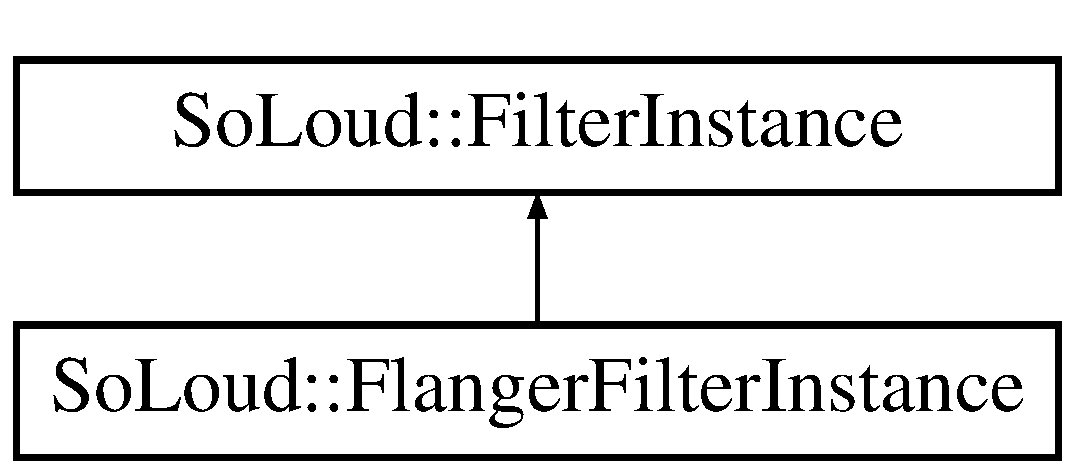
\includegraphics[height=2.000000cm]{class_so_loud_1_1_flanger_filter_instance}
\end{center}
\end{figure}
\subsection*{Public Member Functions}
\begin{DoxyCompactItemize}
\item 
\mbox{\Hypertarget{class_so_loud_1_1_flanger_filter_instance_a9599c24c3a0a917b14bb6da58b3033a6}\label{class_so_loud_1_1_flanger_filter_instance_a9599c24c3a0a917b14bb6da58b3033a6}} 
virtual void {\bfseries filter} (float $\ast$a\+Buffer, unsigned int a\+Samples, unsigned int a\+Channels, float a\+Samplerate, time a\+Time)
\item 
\mbox{\Hypertarget{class_so_loud_1_1_flanger_filter_instance_acb2cc164d3bbfc69d43ebaeb296502f3}\label{class_so_loud_1_1_flanger_filter_instance_acb2cc164d3bbfc69d43ebaeb296502f3}} 
{\bfseries Flanger\+Filter\+Instance} (\mbox{\hyperlink{class_so_loud_1_1_flanger_filter}{Flanger\+Filter}} $\ast$a\+Parent)
\end{DoxyCompactItemize}
\subsection*{Additional Inherited Members}


The documentation for this class was generated from the following file\+:\begin{DoxyCompactItemize}
\item 
deps/\+E\+S\+A\+T/include/\+E\+S\+A\+T\+\_\+extra/soloud/soloud\+\_\+flangerfilter.\+h\end{DoxyCompactItemize}

\hypertarget{class_float2}{}\section{Float2 Class Reference}
\label{class_float2}\index{Float2@{Float2}}
\subsection*{Public Member Functions}
\begin{DoxyCompactItemize}
\item 
\mbox{\Hypertarget{class_float2_acddb9a1528c4bb0eea5d6f5ff394ba22}\label{class_float2_acddb9a1528c4bb0eea5d6f5ff394ba22}} 
{\bfseries Float2} (const float x, const float y)
\item 
\mbox{\Hypertarget{class_float2_ab422f688e2ff254c22836497b4c16e38}\label{class_float2_ab422f688e2ff254c22836497b4c16e38}} 
{\bfseries Float2} (const \mbox{\hyperlink{class_float2}{Float2}} \&o)
\item 
\mbox{\Hypertarget{class_float2_ad68c300eb978ed1a8dec8248595153cd}\label{class_float2_ad68c300eb978ed1a8dec8248595153cd}} 
\mbox{\hyperlink{class_float2}{Float2}} \& {\bfseries operator+=} (const \mbox{\hyperlink{class_float2}{Float2}} \&f)
\item 
\mbox{\Hypertarget{class_float2_accef0e6077301b5162f99a9fca6bf7b2}\label{class_float2_accef0e6077301b5162f99a9fca6bf7b2}} 
\mbox{\hyperlink{class_float2}{Float2}} \& {\bfseries operator-\/=} (const \mbox{\hyperlink{class_float2}{Float2}} \&f)
\item 
\mbox{\Hypertarget{class_float2_a4a5c4efbab76f1c7f8b1c876a30663e4}\label{class_float2_a4a5c4efbab76f1c7f8b1c876a30663e4}} 
\mbox{\hyperlink{class_float2}{Float2}} \& {\bfseries operator$\ast$=} (const \mbox{\hyperlink{class_float2}{Float2}} \&f)
\item 
\mbox{\Hypertarget{class_float2_a9abbc77af852462394ef5a0514d2a782}\label{class_float2_a9abbc77af852462394ef5a0514d2a782}} 
\mbox{\hyperlink{class_float2}{Float2}} \& {\bfseries operator$\ast$=} (float f)
\item 
\mbox{\Hypertarget{class_float2_ae6400fc6994d7bc8925eaa5111d63504}\label{class_float2_ae6400fc6994d7bc8925eaa5111d63504}} 
\mbox{\hyperlink{class_float2}{Float2}} \& {\bfseries operator/=} (const \mbox{\hyperlink{class_float2}{Float2}} \&f)
\item 
\mbox{\Hypertarget{class_float2_a4994310a9af656c23d41d67da206d026}\label{class_float2_a4994310a9af656c23d41d67da206d026}} 
\mbox{\hyperlink{class_float2}{Float2}} \& {\bfseries operator/=} (float f)
\item 
\mbox{\Hypertarget{class_float2_ab59a4832e69acfeb62c5b7105a08bb4f}\label{class_float2_ab59a4832e69acfeb62c5b7105a08bb4f}} 
float {\bfseries Length} () const
\item 
\mbox{\Hypertarget{class_float2_a2e60f4ddef18566c8945d95812c875c6}\label{class_float2_a2e60f4ddef18566c8945d95812c875c6}} 
float {\bfseries Dot\+Product} (const \mbox{\hyperlink{class_float2}{Float2}} \&value) const
\end{DoxyCompactItemize}
\subsection*{Public Attributes}
\begin{DoxyCompactItemize}
\item 
\mbox{\Hypertarget{class_float2_a9f4577102bc9a7bdf9355b5776301485}\label{class_float2_a9f4577102bc9a7bdf9355b5776301485}} 
float {\bfseries x}
\item 
\mbox{\Hypertarget{class_float2_a53deb463e8335f53a8f5454c9c3c0503}\label{class_float2_a53deb463e8335f53a8f5454c9c3c0503}} 
float {\bfseries y}
\end{DoxyCompactItemize}


The documentation for this class was generated from the following file\+:\begin{DoxyCompactItemize}
\item 
deps/\+Math/float2.\+h\end{DoxyCompactItemize}

\hypertarget{structfts5__api}{}\section{fts5\+\_\+api Struct Reference}
\label{structfts5__api}\index{fts5\+\_\+api@{fts5\+\_\+api}}
\subsection*{Public Attributes}
\begin{DoxyCompactItemize}
\item 
\mbox{\Hypertarget{structfts5__api_a3c338289abb33e1805da870172956a7c}\label{structfts5__api_a3c338289abb33e1805da870172956a7c}} 
int {\bfseries i\+Version}
\item 
\mbox{\Hypertarget{structfts5__api_a7fe3663f85eab512d5c461e1674da129}\label{structfts5__api_a7fe3663f85eab512d5c461e1674da129}} 
int($\ast$ {\bfseries x\+Create\+Tokenizer} )(\mbox{\hyperlink{structfts5__api}{fts5\+\_\+api}} $\ast$p\+Api, const char $\ast$z\+Name, void $\ast$p\+Context, \mbox{\hyperlink{structfts5__tokenizer}{fts5\+\_\+tokenizer}} $\ast$p\+Tokenizer, void($\ast$x\+Destroy)(void $\ast$))
\item 
\mbox{\Hypertarget{structfts5__api_a20a23794695fa61e2892ad1243b16b67}\label{structfts5__api_a20a23794695fa61e2892ad1243b16b67}} 
int($\ast$ {\bfseries x\+Find\+Tokenizer} )(\mbox{\hyperlink{structfts5__api}{fts5\+\_\+api}} $\ast$p\+Api, const char $\ast$z\+Name, void $\ast$$\ast$pp\+Context, \mbox{\hyperlink{structfts5__tokenizer}{fts5\+\_\+tokenizer}} $\ast$p\+Tokenizer)
\item 
\mbox{\Hypertarget{structfts5__api_acf1a0612be3b91b908f38ecbc6735d17}\label{structfts5__api_acf1a0612be3b91b908f38ecbc6735d17}} 
int($\ast$ {\bfseries x\+Create\+Function} )(\mbox{\hyperlink{structfts5__api}{fts5\+\_\+api}} $\ast$p\+Api, const char $\ast$z\+Name, void $\ast$p\+Context, fts5\+\_\+extension\+\_\+function x\+Function, void($\ast$x\+Destroy)(void $\ast$))
\end{DoxyCompactItemize}


The documentation for this struct was generated from the following file\+:\begin{DoxyCompactItemize}
\item 
deps/\+E\+S\+A\+T/include/\+E\+S\+A\+T\+\_\+extra/sqlite3.\+h\end{DoxyCompactItemize}

\hypertarget{structfts5__tokenizer}{}\section{fts5\+\_\+tokenizer Struct Reference}
\label{structfts5__tokenizer}\index{fts5\+\_\+tokenizer@{fts5\+\_\+tokenizer}}
\subsection*{Public Attributes}
\begin{DoxyCompactItemize}
\item 
\mbox{\Hypertarget{structfts5__tokenizer_a61846ad000b2d38a1264c342c8201d5c}\label{structfts5__tokenizer_a61846ad000b2d38a1264c342c8201d5c}} 
int($\ast$ {\bfseries x\+Create} )(void $\ast$, const char $\ast$$\ast$az\+Arg, int n\+Arg, Fts5\+Tokenizer $\ast$$\ast$pp\+Out)
\item 
\mbox{\Hypertarget{structfts5__tokenizer_aaaa88b9f3e50f0b1120a05fb1bbb251f}\label{structfts5__tokenizer_aaaa88b9f3e50f0b1120a05fb1bbb251f}} 
void($\ast$ {\bfseries x\+Delete} )(Fts5\+Tokenizer $\ast$)
\item 
\mbox{\Hypertarget{structfts5__tokenizer_ae65ca5a9b1e6d5c1ef09731fccefa577}\label{structfts5__tokenizer_ae65ca5a9b1e6d5c1ef09731fccefa577}} 
int($\ast$ {\bfseries x\+Tokenize} )(Fts5\+Tokenizer $\ast$, void $\ast$p\+Ctx, int flags, const char $\ast$p\+Text, int n\+Text, int($\ast$x\+Token)(void $\ast$p\+Ctx, int tflags, const char $\ast$p\+Token, int n\+Token, int i\+Start, int i\+End))
\end{DoxyCompactItemize}


The documentation for this struct was generated from the following file\+:\begin{DoxyCompactItemize}
\item 
deps/\+E\+S\+A\+T/include/\+E\+S\+A\+T\+\_\+extra/sqlite3.\+h\end{DoxyCompactItemize}

\hypertarget{struct_fts5_extension_api}{}\section{Fts5\+Extension\+Api Struct Reference}
\label{struct_fts5_extension_api}\index{Fts5\+Extension\+Api@{Fts5\+Extension\+Api}}
\subsection*{Public Attributes}
\begin{DoxyCompactItemize}
\item 
\mbox{\Hypertarget{struct_fts5_extension_api_af9c8f09c2e6f1373e6bce57ec9861682}\label{struct_fts5_extension_api_af9c8f09c2e6f1373e6bce57ec9861682}} 
int {\bfseries i\+Version}
\item 
\mbox{\Hypertarget{struct_fts5_extension_api_a8e651288d8e0cf25f20f2b838f47ac34}\label{struct_fts5_extension_api_a8e651288d8e0cf25f20f2b838f47ac34}} 
void $\ast$($\ast$ {\bfseries x\+User\+Data} )(Fts5\+Context $\ast$)
\item 
\mbox{\Hypertarget{struct_fts5_extension_api_a427409c50da4e179c8f2d36b22a4ba21}\label{struct_fts5_extension_api_a427409c50da4e179c8f2d36b22a4ba21}} 
int($\ast$ {\bfseries x\+Column\+Count} )(Fts5\+Context $\ast$)
\item 
\mbox{\Hypertarget{struct_fts5_extension_api_ae1eb7ad1d3c131a09376134ecc099568}\label{struct_fts5_extension_api_ae1eb7ad1d3c131a09376134ecc099568}} 
int($\ast$ {\bfseries x\+Row\+Count} )(Fts5\+Context $\ast$, sqlite3\+\_\+int64 $\ast$pn\+Row)
\item 
\mbox{\Hypertarget{struct_fts5_extension_api_a096e79406ae03df9796a2082d0ac8269}\label{struct_fts5_extension_api_a096e79406ae03df9796a2082d0ac8269}} 
int($\ast$ {\bfseries x\+Column\+Total\+Size} )(Fts5\+Context $\ast$, int i\+Col, sqlite3\+\_\+int64 $\ast$pn\+Token)
\item 
\mbox{\Hypertarget{struct_fts5_extension_api_a670af0d7715f69834376f8df187dcf30}\label{struct_fts5_extension_api_a670af0d7715f69834376f8df187dcf30}} 
int($\ast$ {\bfseries x\+Tokenize} )(Fts5\+Context $\ast$, const char $\ast$p\+Text, int n\+Text, void $\ast$p\+Ctx, int($\ast$x\+Token)(void $\ast$, int, const char $\ast$, int, int, int))
\item 
\mbox{\Hypertarget{struct_fts5_extension_api_a3ba0207080a9ca498625eefcc120bf1e}\label{struct_fts5_extension_api_a3ba0207080a9ca498625eefcc120bf1e}} 
int($\ast$ {\bfseries x\+Phrase\+Count} )(Fts5\+Context $\ast$)
\item 
\mbox{\Hypertarget{struct_fts5_extension_api_aeda6faa66f47f9116c9ceba882aaedd2}\label{struct_fts5_extension_api_aeda6faa66f47f9116c9ceba882aaedd2}} 
int($\ast$ {\bfseries x\+Phrase\+Size} )(Fts5\+Context $\ast$, int i\+Phrase)
\item 
\mbox{\Hypertarget{struct_fts5_extension_api_af57aff7a8aa8402bb37a77892c4daf45}\label{struct_fts5_extension_api_af57aff7a8aa8402bb37a77892c4daf45}} 
int($\ast$ {\bfseries x\+Inst\+Count} )(Fts5\+Context $\ast$, int $\ast$pn\+Inst)
\item 
\mbox{\Hypertarget{struct_fts5_extension_api_a85e17f20db782b20b503f1d803a47a9e}\label{struct_fts5_extension_api_a85e17f20db782b20b503f1d803a47a9e}} 
int($\ast$ {\bfseries x\+Inst} )(Fts5\+Context $\ast$, int i\+Idx, int $\ast$pi\+Phrase, int $\ast$pi\+Col, int $\ast$pi\+Off)
\item 
\mbox{\Hypertarget{struct_fts5_extension_api_acc4336c9f7bf39defa1acbdbf5df0020}\label{struct_fts5_extension_api_acc4336c9f7bf39defa1acbdbf5df0020}} 
sqlite3\+\_\+int64($\ast$ {\bfseries x\+Rowid} )(Fts5\+Context $\ast$)
\item 
\mbox{\Hypertarget{struct_fts5_extension_api_a03c7fcd31a751fc34d25e5288045f91d}\label{struct_fts5_extension_api_a03c7fcd31a751fc34d25e5288045f91d}} 
int($\ast$ {\bfseries x\+Column\+Text} )(Fts5\+Context $\ast$, int i\+Col, const char $\ast$$\ast$pz, int $\ast$pn)
\item 
\mbox{\Hypertarget{struct_fts5_extension_api_aefe6eb4685546e58f056a61da39a2bcb}\label{struct_fts5_extension_api_aefe6eb4685546e58f056a61da39a2bcb}} 
int($\ast$ {\bfseries x\+Column\+Size} )(Fts5\+Context $\ast$, int i\+Col, int $\ast$pn\+Token)
\item 
\mbox{\Hypertarget{struct_fts5_extension_api_a8f6dcf0a1d246b235f98f5bbb214e28d}\label{struct_fts5_extension_api_a8f6dcf0a1d246b235f98f5bbb214e28d}} 
int($\ast$ {\bfseries x\+Query\+Phrase} )(Fts5\+Context $\ast$, int i\+Phrase, void $\ast$p\+User\+Data, int($\ast$)(const \mbox{\hyperlink{struct_fts5_extension_api}{Fts5\+Extension\+Api}} $\ast$, Fts5\+Context $\ast$, void $\ast$))
\item 
\mbox{\Hypertarget{struct_fts5_extension_api_a0f59a6c383a478ed95efdb7e4a95de80}\label{struct_fts5_extension_api_a0f59a6c383a478ed95efdb7e4a95de80}} 
int($\ast$ {\bfseries x\+Set\+Auxdata} )(Fts5\+Context $\ast$, void $\ast$p\+Aux, void($\ast$x\+Delete)(void $\ast$))
\item 
\mbox{\Hypertarget{struct_fts5_extension_api_a63ba9aaf30fe9fe5fbcd1541ff38abff}\label{struct_fts5_extension_api_a63ba9aaf30fe9fe5fbcd1541ff38abff}} 
void $\ast$($\ast$ {\bfseries x\+Get\+Auxdata} )(Fts5\+Context $\ast$, int b\+Clear)
\item 
\mbox{\Hypertarget{struct_fts5_extension_api_a3882208ff21908fc9da1d78b5258b28d}\label{struct_fts5_extension_api_a3882208ff21908fc9da1d78b5258b28d}} 
void($\ast$ {\bfseries x\+Phrase\+First} )(Fts5\+Context $\ast$, int i\+Phrase, \mbox{\hyperlink{struct_fts5_phrase_iter}{Fts5\+Phrase\+Iter}} $\ast$, int $\ast$, int $\ast$)
\item 
\mbox{\Hypertarget{struct_fts5_extension_api_ac46faf7ccccf6a02454069b296dc1877}\label{struct_fts5_extension_api_ac46faf7ccccf6a02454069b296dc1877}} 
void($\ast$ {\bfseries x\+Phrase\+Next} )(Fts5\+Context $\ast$, \mbox{\hyperlink{struct_fts5_phrase_iter}{Fts5\+Phrase\+Iter}} $\ast$, int $\ast$pi\+Col, int $\ast$pi\+Off)
\end{DoxyCompactItemize}


The documentation for this struct was generated from the following file\+:\begin{DoxyCompactItemize}
\item 
deps/\+E\+S\+A\+T/include/\+E\+S\+A\+T\+\_\+extra/sqlite3.\+h\end{DoxyCompactItemize}

\hypertarget{struct_fts5_phrase_iter}{}\section{Fts5\+Phrase\+Iter Struct Reference}
\label{struct_fts5_phrase_iter}\index{Fts5\+Phrase\+Iter@{Fts5\+Phrase\+Iter}}
\subsection*{Public Attributes}
\begin{DoxyCompactItemize}
\item 
\mbox{\Hypertarget{struct_fts5_phrase_iter_a335969d1ac0fcbb94173c472a3f179ae}\label{struct_fts5_phrase_iter_a335969d1ac0fcbb94173c472a3f179ae}} 
const unsigned char $\ast$ {\bfseries a}
\item 
\mbox{\Hypertarget{struct_fts5_phrase_iter_a459180b0d670604aa38b3ac94be6adda}\label{struct_fts5_phrase_iter_a459180b0d670604aa38b3ac94be6adda}} 
const unsigned char $\ast$ {\bfseries b}
\end{DoxyCompactItemize}


The documentation for this struct was generated from the following file\+:\begin{DoxyCompactItemize}
\item 
deps/\+E\+S\+A\+T/include/\+E\+S\+A\+T\+\_\+extra/sqlite3.\+h\end{DoxyCompactItemize}

\hypertarget{class_game_state}{}\section{Game\+State Class Reference}
\label{class_game_state}\index{Game\+State@{Game\+State}}


\mbox{\hyperlink{class_game_state}{Game\+State}} entity.  




{\ttfamily \#include $<$gamestate.\+h$>$}

\subsection*{Static Public Member Functions}
\begin{DoxyCompactItemize}
\item 
static \mbox{\hyperlink{class_game_state}{Game\+State}} \& \mbox{\hyperlink{class_game_state_aaf43c32bcc232594c9e9939c4b55f692}{instance}} ()
\begin{DoxyCompactList}\small\item\em Gets the instance of our \mbox{\hyperlink{class_game_state}{Game\+State}}. \end{DoxyCompactList}\end{DoxyCompactItemize}
\subsection*{Public Attributes}
\begin{DoxyCompactItemize}
\item 
\mbox{\Hypertarget{class_game_state_a17236a9e4ddb53287504198a88c97c59}\label{class_game_state_a17236a9e4ddb53287504198a88c97c59}} 
bool {\bfseries quit\+\_\+game\+\_\+}
\item 
\mbox{\Hypertarget{class_game_state_ac9369dd597cc6276eb96f79c6ebc9ad9}\label{class_game_state_ac9369dd597cc6276eb96f79c6ebc9ad9}} 
uint32\+\_\+t {\bfseries time\+\_\+step\+\_\+}
\item 
\mbox{\Hypertarget{class_game_state_acc35df1f7209e70cbaf971c5128f80cf}\label{class_game_state_acc35df1f7209e70cbaf971c5128f80cf}} 
bool {\bfseries should\+\_\+game\+\_\+end\+\_\+}
\item 
\mbox{\Hypertarget{class_game_state_a17003cbc828a82c99f9454253ca76660}\label{class_game_state_a17003cbc828a82c99f9454253ca76660}} 
E\+S\+A\+T\+::\+Sprite\+Handle {\bfseries agent\+\_\+spr\+\_\+}
\item 
\mbox{\Hypertarget{class_game_state_a25827355b9612be2b489fc41005ea507}\label{class_game_state_a25827355b9612be2b489fc41005ea507}} 
std\+::vector$<$ \mbox{\hyperlink{class_agent}{Agent}} $\ast$ $>$ {\bfseries agents\+\_\+}
\item 
\mbox{\Hypertarget{class_game_state_afd22b13f977d8a6d7ff498c1a38b7845}\label{class_game_state_afd22b13f977d8a6d7ff498c1a38b7845}} 
uint32\+\_\+t {\bfseries frequency\+\_\+}
\end{DoxyCompactItemize}


\subsection{Detailed Description}
\mbox{\hyperlink{class_game_state}{Game\+State}} entity. 

Game State of our game based in a Singleton pattern. 

\subsection{Member Function Documentation}
\mbox{\Hypertarget{class_game_state_aaf43c32bcc232594c9e9939c4b55f692}\label{class_game_state_aaf43c32bcc232594c9e9939c4b55f692}} 
\index{Game\+State@{Game\+State}!instance@{instance}}
\index{instance@{instance}!Game\+State@{Game\+State}}
\subsubsection{\texorpdfstring{instance()}{instance()}}
{\footnotesize\ttfamily static \mbox{\hyperlink{class_game_state}{Game\+State}}\& Game\+State\+::instance (\begin{DoxyParamCaption}{ }\end{DoxyParamCaption})\hspace{0.3cm}{\ttfamily [static]}}



Gets the instance of our \mbox{\hyperlink{class_game_state}{Game\+State}}. 

In charge of creating our \mbox{\hyperlink{class_game_state}{Game\+State}} singleton in case it does not exist or return its instance if it exists.

\begin{DoxyReturn}{Returns}
\mbox{\hyperlink{class_game_state}{Game\+State}}\& instance 
\end{DoxyReturn}


The documentation for this class was generated from the following file\+:\begin{DoxyCompactItemize}
\item 
E\+:/\+Pepe/\+E\+S\+A\+T/\+I\+A/3ia\+\_\+ta\+\_\+martinezcajm/include/gamestate.\+h\end{DoxyCompactItemize}

\hypertarget{struct_im_font_1_1_glyph}{}\section{Im\+Font\+:\+:Glyph Struct Reference}
\label{struct_im_font_1_1_glyph}\index{Im\+Font\+::\+Glyph@{Im\+Font\+::\+Glyph}}
\subsection*{Public Attributes}
\begin{DoxyCompactItemize}
\item 
\mbox{\Hypertarget{struct_im_font_1_1_glyph_a9d612199d341de86cb7b0c33539b4830}\label{struct_im_font_1_1_glyph_a9d612199d341de86cb7b0c33539b4830}} 
Im\+Wchar {\bfseries Codepoint}
\item 
\mbox{\Hypertarget{struct_im_font_1_1_glyph_ab09eb257d6cc68385654a25ba167894f}\label{struct_im_font_1_1_glyph_ab09eb257d6cc68385654a25ba167894f}} 
float {\bfseries X\+Advance}
\item 
\mbox{\Hypertarget{struct_im_font_1_1_glyph_ae4e362012824c54d41ff7fbff46cf88b}\label{struct_im_font_1_1_glyph_ae4e362012824c54d41ff7fbff46cf88b}} 
float {\bfseries X0}
\item 
\mbox{\Hypertarget{struct_im_font_1_1_glyph_ad7f9c0b94f16cecb62109d5a73d8cb8b}\label{struct_im_font_1_1_glyph_ad7f9c0b94f16cecb62109d5a73d8cb8b}} 
float {\bfseries Y0}
\item 
\mbox{\Hypertarget{struct_im_font_1_1_glyph_ac1e7bc71d1f235fe3c993ba163e65f56}\label{struct_im_font_1_1_glyph_ac1e7bc71d1f235fe3c993ba163e65f56}} 
float {\bfseries X1}
\item 
\mbox{\Hypertarget{struct_im_font_1_1_glyph_ab5e51179eeaef0849befcbf69ecaa669}\label{struct_im_font_1_1_glyph_ab5e51179eeaef0849befcbf69ecaa669}} 
float {\bfseries Y1}
\item 
\mbox{\Hypertarget{struct_im_font_1_1_glyph_a6e78ab35f36e7eee16c85e60eb9d445a}\label{struct_im_font_1_1_glyph_a6e78ab35f36e7eee16c85e60eb9d445a}} 
float {\bfseries U0}
\item 
\mbox{\Hypertarget{struct_im_font_1_1_glyph_a7de7fe9f4420b1c8336419a1739ff20a}\label{struct_im_font_1_1_glyph_a7de7fe9f4420b1c8336419a1739ff20a}} 
float {\bfseries V0}
\item 
\mbox{\Hypertarget{struct_im_font_1_1_glyph_a9e443ec24dc105b512ae57737e43af84}\label{struct_im_font_1_1_glyph_a9e443ec24dc105b512ae57737e43af84}} 
float {\bfseries U1}
\item 
\mbox{\Hypertarget{struct_im_font_1_1_glyph_a803ff02b149bd2795f3d90fc601706ef}\label{struct_im_font_1_1_glyph_a803ff02b149bd2795f3d90fc601706ef}} 
float {\bfseries V1}
\end{DoxyCompactItemize}


The documentation for this struct was generated from the following file\+:\begin{DoxyCompactItemize}
\item 
deps/\+E\+S\+A\+T/include/\+E\+S\+A\+T\+\_\+extra/imgui.\+h\end{DoxyCompactItemize}

\hypertarget{struct_im_color}{}\section{Im\+Color Struct Reference}
\label{struct_im_color}\index{Im\+Color@{Im\+Color}}
\subsection*{Public Member Functions}
\begin{DoxyCompactItemize}
\item 
\mbox{\Hypertarget{struct_im_color_ab4ba02f8290d5dadc1ebc57b2c8a9cbe}\label{struct_im_color_ab4ba02f8290d5dadc1ebc57b2c8a9cbe}} 
{\bfseries Im\+Color} (int r, int g, int b, int a=255)
\item 
\mbox{\Hypertarget{struct_im_color_ad306332841a2b1f903f40262a19f9412}\label{struct_im_color_ad306332841a2b1f903f40262a19f9412}} 
{\bfseries Im\+Color} (Im\+U32 rgba)
\item 
\mbox{\Hypertarget{struct_im_color_a92b53917ca9d90a7207b18270ff5453d}\label{struct_im_color_a92b53917ca9d90a7207b18270ff5453d}} 
{\bfseries Im\+Color} (float r, float g, float b, float a=1.\+0f)
\item 
\mbox{\Hypertarget{struct_im_color_aa5306926b3ef766a8647b26bdfd9f8d2}\label{struct_im_color_aa5306926b3ef766a8647b26bdfd9f8d2}} 
{\bfseries Im\+Color} (const \mbox{\hyperlink{struct_im_vec4}{Im\+Vec4}} \&col)
\item 
\mbox{\Hypertarget{struct_im_color_a4f4fc53e0676d50404d6d5ffcf16637f}\label{struct_im_color_a4f4fc53e0676d50404d6d5ffcf16637f}} 
{\bfseries operator Im\+U32} () const
\item 
\mbox{\Hypertarget{struct_im_color_a10f1de242f13c93f8be64545e4cbcb0a}\label{struct_im_color_a10f1de242f13c93f8be64545e4cbcb0a}} 
{\bfseries operator Im\+Vec4} () const
\item 
\mbox{\Hypertarget{struct_im_color_afcff20160db703b956d56e5a9fa88e24}\label{struct_im_color_afcff20160db703b956d56e5a9fa88e24}} 
void {\bfseries Set\+H\+SV} (float h, float s, float v, float a=1.\+0f)
\end{DoxyCompactItemize}
\subsection*{Static Public Member Functions}
\begin{DoxyCompactItemize}
\item 
\mbox{\Hypertarget{struct_im_color_ac8cb52119648523038818a613becf010}\label{struct_im_color_ac8cb52119648523038818a613becf010}} 
static \mbox{\hyperlink{struct_im_color}{Im\+Color}} {\bfseries H\+SV} (float h, float s, float v, float a=1.\+0f)
\end{DoxyCompactItemize}
\subsection*{Public Attributes}
\begin{DoxyCompactItemize}
\item 
\mbox{\Hypertarget{struct_im_color_a4cf43bd58e30decaa0248f839fc85e95}\label{struct_im_color_a4cf43bd58e30decaa0248f839fc85e95}} 
\mbox{\hyperlink{struct_im_vec4}{Im\+Vec4}} {\bfseries Value}
\end{DoxyCompactItemize}


The documentation for this struct was generated from the following file\+:\begin{DoxyCompactItemize}
\item 
deps/\+E\+S\+A\+T/include/\+E\+S\+A\+T\+\_\+extra/imgui.\+h\end{DoxyCompactItemize}

\hypertarget{struct_im_draw_channel}{}\section{Im\+Draw\+Channel Struct Reference}
\label{struct_im_draw_channel}\index{Im\+Draw\+Channel@{Im\+Draw\+Channel}}
\subsection*{Public Attributes}
\begin{DoxyCompactItemize}
\item 
\mbox{\Hypertarget{struct_im_draw_channel_abdaa17053d55fb6757c1971d410ceddf}\label{struct_im_draw_channel_abdaa17053d55fb6757c1971d410ceddf}} 
\mbox{\hyperlink{class_im_vector}{Im\+Vector}}$<$ \mbox{\hyperlink{struct_im_draw_cmd}{Im\+Draw\+Cmd}} $>$ {\bfseries Cmd\+Buffer}
\item 
\mbox{\Hypertarget{struct_im_draw_channel_a7fbed7d3523124fadd94859d5ac0fd67}\label{struct_im_draw_channel_a7fbed7d3523124fadd94859d5ac0fd67}} 
\mbox{\hyperlink{class_im_vector}{Im\+Vector}}$<$ Im\+Draw\+Idx $>$ {\bfseries Idx\+Buffer}
\end{DoxyCompactItemize}


The documentation for this struct was generated from the following file\+:\begin{DoxyCompactItemize}
\item 
deps/\+E\+S\+A\+T/include/\+E\+S\+A\+T\+\_\+extra/imgui.\+h\end{DoxyCompactItemize}

\hypertarget{struct_im_draw_cmd}{}\section{Im\+Draw\+Cmd Struct Reference}
\label{struct_im_draw_cmd}\index{Im\+Draw\+Cmd@{Im\+Draw\+Cmd}}
\subsection*{Public Attributes}
\begin{DoxyCompactItemize}
\item 
\mbox{\Hypertarget{struct_im_draw_cmd_aafe2532964fb1f6905d67d84dd3e8730}\label{struct_im_draw_cmd_aafe2532964fb1f6905d67d84dd3e8730}} 
unsigned int {\bfseries Elem\+Count}
\item 
\mbox{\Hypertarget{struct_im_draw_cmd_a838918f420ff81cb8dc7265077592daa}\label{struct_im_draw_cmd_a838918f420ff81cb8dc7265077592daa}} 
\mbox{\hyperlink{struct_im_vec4}{Im\+Vec4}} {\bfseries Clip\+Rect}
\item 
\mbox{\Hypertarget{struct_im_draw_cmd_a4f3b5985ece9ca6b71e7a8e7d85a82e5}\label{struct_im_draw_cmd_a4f3b5985ece9ca6b71e7a8e7d85a82e5}} 
Im\+Texture\+ID {\bfseries Texture\+Id}
\item 
\mbox{\Hypertarget{struct_im_draw_cmd_ad26dac4e939f5c4bb892cbca0f9e3af8}\label{struct_im_draw_cmd_ad26dac4e939f5c4bb892cbca0f9e3af8}} 
Im\+Draw\+Callback {\bfseries User\+Callback}
\item 
\mbox{\Hypertarget{struct_im_draw_cmd_ae2f5a0baf4a0b25942237b8ce6adb42d}\label{struct_im_draw_cmd_ae2f5a0baf4a0b25942237b8ce6adb42d}} 
void $\ast$ {\bfseries User\+Callback\+Data}
\end{DoxyCompactItemize}


The documentation for this struct was generated from the following file\+:\begin{DoxyCompactItemize}
\item 
deps/\+E\+S\+A\+T/include/\+E\+S\+A\+T\+\_\+extra/imgui.\+h\end{DoxyCompactItemize}

\hypertarget{struct_im_draw_data}{}\section{Im\+Draw\+Data Struct Reference}
\label{struct_im_draw_data}\index{Im\+Draw\+Data@{Im\+Draw\+Data}}
\subsection*{Public Member Functions}
\begin{DoxyCompactItemize}
\item 
\mbox{\Hypertarget{struct_im_draw_data_af75033bfd13b36910487af2f28e0c912}\label{struct_im_draw_data_af75033bfd13b36910487af2f28e0c912}} 
I\+M\+G\+U\+I\+\_\+\+A\+PI void {\bfseries De\+Index\+All\+Buffers} ()
\item 
\mbox{\Hypertarget{struct_im_draw_data_af162d01f17a909f6b9c07001282682ed}\label{struct_im_draw_data_af162d01f17a909f6b9c07001282682ed}} 
I\+M\+G\+U\+I\+\_\+\+A\+PI void {\bfseries Scale\+Clip\+Rects} (const \mbox{\hyperlink{struct_im_vec2}{Im\+Vec2}} \&sc)
\end{DoxyCompactItemize}
\subsection*{Public Attributes}
\begin{DoxyCompactItemize}
\item 
\mbox{\Hypertarget{struct_im_draw_data_ad01ab9ce5e8843b7860ccbb3eb9a6554}\label{struct_im_draw_data_ad01ab9ce5e8843b7860ccbb3eb9a6554}} 
bool {\bfseries Valid}
\item 
\mbox{\Hypertarget{struct_im_draw_data_a9e93fe7e620eb2e9f61e3b689d617edc}\label{struct_im_draw_data_a9e93fe7e620eb2e9f61e3b689d617edc}} 
\mbox{\hyperlink{struct_im_draw_list}{Im\+Draw\+List}} $\ast$$\ast$ {\bfseries Cmd\+Lists}
\item 
\mbox{\Hypertarget{struct_im_draw_data_adc0bbc2881c15f78bdabe51d82582f4e}\label{struct_im_draw_data_adc0bbc2881c15f78bdabe51d82582f4e}} 
int {\bfseries Cmd\+Lists\+Count}
\item 
\mbox{\Hypertarget{struct_im_draw_data_af0035b52cdf91932b25eaf2da853965a}\label{struct_im_draw_data_af0035b52cdf91932b25eaf2da853965a}} 
int {\bfseries Total\+Vtx\+Count}
\item 
\mbox{\Hypertarget{struct_im_draw_data_a1ac8a5d441f464628295ef91a0602fc5}\label{struct_im_draw_data_a1ac8a5d441f464628295ef91a0602fc5}} 
int {\bfseries Total\+Idx\+Count}
\end{DoxyCompactItemize}


The documentation for this struct was generated from the following file\+:\begin{DoxyCompactItemize}
\item 
deps/\+E\+S\+A\+T/include/\+E\+S\+A\+T\+\_\+extra/imgui.\+h\end{DoxyCompactItemize}

\hypertarget{struct_im_draw_list}{}\section{Im\+Draw\+List Struct Reference}
\label{struct_im_draw_list}\index{Im\+Draw\+List@{Im\+Draw\+List}}
\subsection*{Public Member Functions}
\begin{DoxyCompactItemize}
\item 
\mbox{\Hypertarget{struct_im_draw_list_a87e19224a2628a6c6dae483b33b59c87}\label{struct_im_draw_list_a87e19224a2628a6c6dae483b33b59c87}} 
I\+M\+G\+U\+I\+\_\+\+A\+PI void {\bfseries Push\+Clip\+Rect} (const \mbox{\hyperlink{struct_im_vec4}{Im\+Vec4}} \&clip\+\_\+rect)
\item 
\mbox{\Hypertarget{struct_im_draw_list_a487aa3b1496dac28060baaaea593d23d}\label{struct_im_draw_list_a487aa3b1496dac28060baaaea593d23d}} 
I\+M\+G\+U\+I\+\_\+\+A\+PI void {\bfseries Push\+Clip\+Rect\+Full\+Screen} ()
\item 
\mbox{\Hypertarget{struct_im_draw_list_a717568372b45f1088036abd35315ca77}\label{struct_im_draw_list_a717568372b45f1088036abd35315ca77}} 
I\+M\+G\+U\+I\+\_\+\+A\+PI void {\bfseries Pop\+Clip\+Rect} ()
\item 
\mbox{\Hypertarget{struct_im_draw_list_a07e9041d53c2d1204774ca7c13b061f1}\label{struct_im_draw_list_a07e9041d53c2d1204774ca7c13b061f1}} 
I\+M\+G\+U\+I\+\_\+\+A\+PI void {\bfseries Push\+Texture\+ID} (const Im\+Texture\+ID \&texture\+\_\+id)
\item 
\mbox{\Hypertarget{struct_im_draw_list_af7dff1e6fd55e868107b4b52c66cd02a}\label{struct_im_draw_list_af7dff1e6fd55e868107b4b52c66cd02a}} 
I\+M\+G\+U\+I\+\_\+\+A\+PI void {\bfseries Pop\+Texture\+ID} ()
\item 
\mbox{\Hypertarget{struct_im_draw_list_a2d5b8eb5ae58ef58c370a8c9b6154f2a}\label{struct_im_draw_list_a2d5b8eb5ae58ef58c370a8c9b6154f2a}} 
I\+M\+G\+U\+I\+\_\+\+A\+PI void {\bfseries Add\+Line} (const \mbox{\hyperlink{struct_im_vec2}{Im\+Vec2}} \&a, const \mbox{\hyperlink{struct_im_vec2}{Im\+Vec2}} \&b, Im\+U32 col, float thickness=1.\+0f)
\item 
\mbox{\Hypertarget{struct_im_draw_list_afcbce9cf6ccd4db612528d218b0545fa}\label{struct_im_draw_list_afcbce9cf6ccd4db612528d218b0545fa}} 
I\+M\+G\+U\+I\+\_\+\+A\+PI void {\bfseries Add\+Rect} (const \mbox{\hyperlink{struct_im_vec2}{Im\+Vec2}} \&a, const \mbox{\hyperlink{struct_im_vec2}{Im\+Vec2}} \&b, Im\+U32 col, float rounding=0.\+0f, int rounding\+\_\+corners=0x0\+F, float thickness=1.\+0f)
\item 
\mbox{\Hypertarget{struct_im_draw_list_ab611dd9a03b878f3cc7db25c403b5766}\label{struct_im_draw_list_ab611dd9a03b878f3cc7db25c403b5766}} 
I\+M\+G\+U\+I\+\_\+\+A\+PI void {\bfseries Add\+Rect\+Filled} (const \mbox{\hyperlink{struct_im_vec2}{Im\+Vec2}} \&a, const \mbox{\hyperlink{struct_im_vec2}{Im\+Vec2}} \&b, Im\+U32 col, float rounding=0.\+0f, int rounding\+\_\+corners=0x0\+F)
\item 
\mbox{\Hypertarget{struct_im_draw_list_af8e1758e416bacfdbac38043a85c364b}\label{struct_im_draw_list_af8e1758e416bacfdbac38043a85c364b}} 
I\+M\+G\+U\+I\+\_\+\+A\+PI void {\bfseries Add\+Rect\+Filled\+Multi\+Color} (const \mbox{\hyperlink{struct_im_vec2}{Im\+Vec2}} \&a, const \mbox{\hyperlink{struct_im_vec2}{Im\+Vec2}} \&b, Im\+U32 col\+\_\+upr\+\_\+left, Im\+U32 col\+\_\+upr\+\_\+right, Im\+U32 col\+\_\+bot\+\_\+right, Im\+U32 col\+\_\+bot\+\_\+left)
\item 
\mbox{\Hypertarget{struct_im_draw_list_a4954e6ea71858501270a80daaf087a9a}\label{struct_im_draw_list_a4954e6ea71858501270a80daaf087a9a}} 
I\+M\+G\+U\+I\+\_\+\+A\+PI void {\bfseries Add\+Triangle} (const \mbox{\hyperlink{struct_im_vec2}{Im\+Vec2}} \&a, const \mbox{\hyperlink{struct_im_vec2}{Im\+Vec2}} \&b, const \mbox{\hyperlink{struct_im_vec2}{Im\+Vec2}} \&c, Im\+U32 col, float thickness=1.\+0f)
\item 
\mbox{\Hypertarget{struct_im_draw_list_ad046c71c7d5e4dbe5506c0a1f794fc2e}\label{struct_im_draw_list_ad046c71c7d5e4dbe5506c0a1f794fc2e}} 
I\+M\+G\+U\+I\+\_\+\+A\+PI void {\bfseries Add\+Triangle\+Filled} (const \mbox{\hyperlink{struct_im_vec2}{Im\+Vec2}} \&a, const \mbox{\hyperlink{struct_im_vec2}{Im\+Vec2}} \&b, const \mbox{\hyperlink{struct_im_vec2}{Im\+Vec2}} \&c, Im\+U32 col)
\item 
\mbox{\Hypertarget{struct_im_draw_list_adeb4dd03bd2004a94ef13f54d5526b41}\label{struct_im_draw_list_adeb4dd03bd2004a94ef13f54d5526b41}} 
I\+M\+G\+U\+I\+\_\+\+A\+PI void {\bfseries Add\+Circle} (const \mbox{\hyperlink{struct_im_vec2}{Im\+Vec2}} \&centre, float radius, Im\+U32 col, int num\+\_\+segments=12, float thickness=1.\+0f)
\item 
\mbox{\Hypertarget{struct_im_draw_list_a69ace164b2e5d949b09e299606cc77da}\label{struct_im_draw_list_a69ace164b2e5d949b09e299606cc77da}} 
I\+M\+G\+U\+I\+\_\+\+A\+PI void {\bfseries Add\+Circle\+Filled} (const \mbox{\hyperlink{struct_im_vec2}{Im\+Vec2}} \&centre, float radius, Im\+U32 col, int num\+\_\+segments=12)
\item 
\mbox{\Hypertarget{struct_im_draw_list_abd3ce88c86a20632f89d9ac324b02b51}\label{struct_im_draw_list_abd3ce88c86a20632f89d9ac324b02b51}} 
I\+M\+G\+U\+I\+\_\+\+A\+PI void {\bfseries Add\+Text} (const \mbox{\hyperlink{struct_im_vec2}{Im\+Vec2}} \&pos, Im\+U32 col, const char $\ast$text\+\_\+begin, const char $\ast$text\+\_\+end=N\+U\+LL)
\item 
\mbox{\Hypertarget{struct_im_draw_list_a8998356210b4c6c063a71a4af890d3fd}\label{struct_im_draw_list_a8998356210b4c6c063a71a4af890d3fd}} 
I\+M\+G\+U\+I\+\_\+\+A\+PI void {\bfseries Add\+Text} (const \mbox{\hyperlink{struct_im_font}{Im\+Font}} $\ast$font, float font\+\_\+size, const \mbox{\hyperlink{struct_im_vec2}{Im\+Vec2}} \&pos, Im\+U32 col, const char $\ast$text\+\_\+begin, const char $\ast$text\+\_\+end=N\+U\+LL, float wrap\+\_\+width=0.\+0f, const Im\+Vec4 $\ast$cpu\+\_\+fine\+\_\+clip\+\_\+rect=\+N\+U\+L\+L)
\item 
\mbox{\Hypertarget{struct_im_draw_list_a56f40a2a8d5f309a4c032aac70e1a765}\label{struct_im_draw_list_a56f40a2a8d5f309a4c032aac70e1a765}} 
I\+M\+G\+U\+I\+\_\+\+A\+PI void {\bfseries Add\+Image} (Im\+Texture\+ID user\+\_\+texture\+\_\+id, const \mbox{\hyperlink{struct_im_vec2}{Im\+Vec2}} \&a, const \mbox{\hyperlink{struct_im_vec2}{Im\+Vec2}} \&b, const \mbox{\hyperlink{struct_im_vec2}{Im\+Vec2}} \&uv0=\mbox{\hyperlink{struct_im_vec2}{Im\+Vec2}}(0, 0), const \mbox{\hyperlink{struct_im_vec2}{Im\+Vec2}} \&uv1=\mbox{\hyperlink{struct_im_vec2}{Im\+Vec2}}(1, 1), Im\+U32 col=0x\+F\+F\+F\+F\+F\+F\+F\+F)
\item 
\mbox{\Hypertarget{struct_im_draw_list_a77b2dae2d0b7c1498b8844abb87308a6}\label{struct_im_draw_list_a77b2dae2d0b7c1498b8844abb87308a6}} 
I\+M\+G\+U\+I\+\_\+\+A\+PI void {\bfseries Add\+Polyline} (const \mbox{\hyperlink{struct_im_vec2}{Im\+Vec2}} $\ast$points, const int num\+\_\+points, Im\+U32 col, bool closed, float thickness, bool anti\+\_\+aliased)
\item 
\mbox{\Hypertarget{struct_im_draw_list_ac5df2073259ae2ca1797838835004ed8}\label{struct_im_draw_list_ac5df2073259ae2ca1797838835004ed8}} 
I\+M\+G\+U\+I\+\_\+\+A\+PI void {\bfseries Add\+Convex\+Poly\+Filled} (const \mbox{\hyperlink{struct_im_vec2}{Im\+Vec2}} $\ast$points, const int num\+\_\+points, Im\+U32 col, bool anti\+\_\+aliased)
\item 
\mbox{\Hypertarget{struct_im_draw_list_a990409b6456377fdf4578082a468a378}\label{struct_im_draw_list_a990409b6456377fdf4578082a468a378}} 
I\+M\+G\+U\+I\+\_\+\+A\+PI void {\bfseries Add\+Bezier\+Curve} (const \mbox{\hyperlink{struct_im_vec2}{Im\+Vec2}} \&pos0, const \mbox{\hyperlink{struct_im_vec2}{Im\+Vec2}} \&cp0, const \mbox{\hyperlink{struct_im_vec2}{Im\+Vec2}} \&cp1, const \mbox{\hyperlink{struct_im_vec2}{Im\+Vec2}} \&pos1, Im\+U32 col, float thickness, int num\+\_\+segments=0)
\item 
\mbox{\Hypertarget{struct_im_draw_list_ae9ad5f4d638b1bfd9383618dc60e3f18}\label{struct_im_draw_list_ae9ad5f4d638b1bfd9383618dc60e3f18}} 
void {\bfseries Path\+Clear} ()
\item 
\mbox{\Hypertarget{struct_im_draw_list_a828d944325ed58d8b57abd3647bffaaf}\label{struct_im_draw_list_a828d944325ed58d8b57abd3647bffaaf}} 
void {\bfseries Path\+Line\+To} (const \mbox{\hyperlink{struct_im_vec2}{Im\+Vec2}} \&pos)
\item 
\mbox{\Hypertarget{struct_im_draw_list_aa3dd11945fb62495f8b9e1392ed724e3}\label{struct_im_draw_list_aa3dd11945fb62495f8b9e1392ed724e3}} 
void {\bfseries Path\+Line\+To\+Merge\+Duplicate} (const \mbox{\hyperlink{struct_im_vec2}{Im\+Vec2}} \&pos)
\item 
\mbox{\Hypertarget{struct_im_draw_list_ac23cb368464d1c98230d1bf44e469c4f}\label{struct_im_draw_list_ac23cb368464d1c98230d1bf44e469c4f}} 
void {\bfseries Path\+Fill} (Im\+U32 col)
\item 
\mbox{\Hypertarget{struct_im_draw_list_ac3172e376a4b77915bb22b6d8092b8b2}\label{struct_im_draw_list_ac3172e376a4b77915bb22b6d8092b8b2}} 
void {\bfseries Path\+Stroke} (Im\+U32 col, bool closed, float thickness=1.\+0f)
\item 
\mbox{\Hypertarget{struct_im_draw_list_a66744510ad42701992fecc009320e632}\label{struct_im_draw_list_a66744510ad42701992fecc009320e632}} 
I\+M\+G\+U\+I\+\_\+\+A\+PI void {\bfseries Path\+Arc\+To} (const \mbox{\hyperlink{struct_im_vec2}{Im\+Vec2}} \&centre, float radius, float a\+\_\+min, float a\+\_\+max, int num\+\_\+segments=10)
\item 
\mbox{\Hypertarget{struct_im_draw_list_aa40b230336239ca99ae84657017c8ebb}\label{struct_im_draw_list_aa40b230336239ca99ae84657017c8ebb}} 
I\+M\+G\+U\+I\+\_\+\+A\+PI void {\bfseries Path\+Arc\+To\+Fast} (const \mbox{\hyperlink{struct_im_vec2}{Im\+Vec2}} \&centre, float radius, int a\+\_\+min\+\_\+of\+\_\+12, int a\+\_\+max\+\_\+of\+\_\+12)
\item 
\mbox{\Hypertarget{struct_im_draw_list_a7534ffbc60761e2893444b6c11d83a28}\label{struct_im_draw_list_a7534ffbc60761e2893444b6c11d83a28}} 
I\+M\+G\+U\+I\+\_\+\+A\+PI void {\bfseries Path\+Bezier\+Curve\+To} (const \mbox{\hyperlink{struct_im_vec2}{Im\+Vec2}} \&p1, const \mbox{\hyperlink{struct_im_vec2}{Im\+Vec2}} \&p2, const \mbox{\hyperlink{struct_im_vec2}{Im\+Vec2}} \&p3, int num\+\_\+segments=0)
\item 
\mbox{\Hypertarget{struct_im_draw_list_a876f4d327502bebec04d4cfbc9d1fc13}\label{struct_im_draw_list_a876f4d327502bebec04d4cfbc9d1fc13}} 
I\+M\+G\+U\+I\+\_\+\+A\+PI void {\bfseries Path\+Rect} (const \mbox{\hyperlink{struct_im_vec2}{Im\+Vec2}} \&rect\+\_\+min, const \mbox{\hyperlink{struct_im_vec2}{Im\+Vec2}} \&rect\+\_\+max, float rounding=0.\+0f, int rounding\+\_\+corners=0x0\+F)
\item 
\mbox{\Hypertarget{struct_im_draw_list_aaab6835f0fb17a79510cbb057ad15cad}\label{struct_im_draw_list_aaab6835f0fb17a79510cbb057ad15cad}} 
I\+M\+G\+U\+I\+\_\+\+A\+PI void {\bfseries Channels\+Split} (int channels\+\_\+count)
\item 
\mbox{\Hypertarget{struct_im_draw_list_a5296cbc4ba6ccdbfbe62ef6b4fc76468}\label{struct_im_draw_list_a5296cbc4ba6ccdbfbe62ef6b4fc76468}} 
I\+M\+G\+U\+I\+\_\+\+A\+PI void {\bfseries Channels\+Merge} ()
\item 
\mbox{\Hypertarget{struct_im_draw_list_a460072bcefc25e5e8052903173de67f5}\label{struct_im_draw_list_a460072bcefc25e5e8052903173de67f5}} 
I\+M\+G\+U\+I\+\_\+\+A\+PI void {\bfseries Channels\+Set\+Current} (int channel\+\_\+index)
\item 
\mbox{\Hypertarget{struct_im_draw_list_a04e9c88972cde170e257f04cc5cf73c8}\label{struct_im_draw_list_a04e9c88972cde170e257f04cc5cf73c8}} 
I\+M\+G\+U\+I\+\_\+\+A\+PI void {\bfseries Add\+Callback} (Im\+Draw\+Callback callback, void $\ast$callback\+\_\+data)
\item 
\mbox{\Hypertarget{struct_im_draw_list_a5ad8fac0b8e76be9a7cde77637d6bca2}\label{struct_im_draw_list_a5ad8fac0b8e76be9a7cde77637d6bca2}} 
I\+M\+G\+U\+I\+\_\+\+A\+PI void {\bfseries Add\+Draw\+Cmd} ()
\item 
\mbox{\Hypertarget{struct_im_draw_list_a611458546f5ceeeef6150376e9f61d44}\label{struct_im_draw_list_a611458546f5ceeeef6150376e9f61d44}} 
I\+M\+G\+U\+I\+\_\+\+A\+PI void {\bfseries Clear} ()
\item 
\mbox{\Hypertarget{struct_im_draw_list_a6edeb43d626c0701341abe7301a79323}\label{struct_im_draw_list_a6edeb43d626c0701341abe7301a79323}} 
I\+M\+G\+U\+I\+\_\+\+A\+PI void {\bfseries Clear\+Free\+Memory} ()
\item 
\mbox{\Hypertarget{struct_im_draw_list_a507a691f33d12bbfd2b4c16756f4fb31}\label{struct_im_draw_list_a507a691f33d12bbfd2b4c16756f4fb31}} 
I\+M\+G\+U\+I\+\_\+\+A\+PI void {\bfseries Prim\+Reserve} (int idx\+\_\+count, int vtx\+\_\+count)
\item 
\mbox{\Hypertarget{struct_im_draw_list_a30d56ec472ae78be87861358bc81f821}\label{struct_im_draw_list_a30d56ec472ae78be87861358bc81f821}} 
I\+M\+G\+U\+I\+\_\+\+A\+PI void {\bfseries Prim\+Rect} (const \mbox{\hyperlink{struct_im_vec2}{Im\+Vec2}} \&a, const \mbox{\hyperlink{struct_im_vec2}{Im\+Vec2}} \&b, Im\+U32 col)
\item 
\mbox{\Hypertarget{struct_im_draw_list_adb963875428136a436a0faef556c810c}\label{struct_im_draw_list_adb963875428136a436a0faef556c810c}} 
I\+M\+G\+U\+I\+\_\+\+A\+PI void {\bfseries Prim\+Rect\+UV} (const \mbox{\hyperlink{struct_im_vec2}{Im\+Vec2}} \&a, const \mbox{\hyperlink{struct_im_vec2}{Im\+Vec2}} \&b, const \mbox{\hyperlink{struct_im_vec2}{Im\+Vec2}} \&uv\+\_\+a, const \mbox{\hyperlink{struct_im_vec2}{Im\+Vec2}} \&uv\+\_\+b, Im\+U32 col)
\item 
\mbox{\Hypertarget{struct_im_draw_list_a9779645708cc70814f6caebaffdbf781}\label{struct_im_draw_list_a9779645708cc70814f6caebaffdbf781}} 
I\+M\+G\+U\+I\+\_\+\+A\+PI void {\bfseries Prim\+Quad\+UV} (const \mbox{\hyperlink{struct_im_vec2}{Im\+Vec2}} \&a, const \mbox{\hyperlink{struct_im_vec2}{Im\+Vec2}} \&b, const \mbox{\hyperlink{struct_im_vec2}{Im\+Vec2}} \&c, const \mbox{\hyperlink{struct_im_vec2}{Im\+Vec2}} \&d, const \mbox{\hyperlink{struct_im_vec2}{Im\+Vec2}} \&uv\+\_\+a, const \mbox{\hyperlink{struct_im_vec2}{Im\+Vec2}} \&uv\+\_\+b, const \mbox{\hyperlink{struct_im_vec2}{Im\+Vec2}} \&uv\+\_\+c, const \mbox{\hyperlink{struct_im_vec2}{Im\+Vec2}} \&uv\+\_\+d, Im\+U32 col)
\item 
\mbox{\Hypertarget{struct_im_draw_list_a405377158f0028ad8b4fb6509eef4532}\label{struct_im_draw_list_a405377158f0028ad8b4fb6509eef4532}} 
void {\bfseries Prim\+Vtx} (const \mbox{\hyperlink{struct_im_vec2}{Im\+Vec2}} \&pos, const \mbox{\hyperlink{struct_im_vec2}{Im\+Vec2}} \&uv, Im\+U32 col)
\item 
\mbox{\Hypertarget{struct_im_draw_list_af86de4faf6c8e978fb712ea14c5d0c5f}\label{struct_im_draw_list_af86de4faf6c8e978fb712ea14c5d0c5f}} 
void {\bfseries Prim\+Write\+Vtx} (const \mbox{\hyperlink{struct_im_vec2}{Im\+Vec2}} \&pos, const \mbox{\hyperlink{struct_im_vec2}{Im\+Vec2}} \&uv, Im\+U32 col)
\item 
\mbox{\Hypertarget{struct_im_draw_list_a42b72f87a0084c02f11dcd1560c8bbc7}\label{struct_im_draw_list_a42b72f87a0084c02f11dcd1560c8bbc7}} 
void {\bfseries Prim\+Write\+Idx} (Im\+Draw\+Idx idx)
\item 
\mbox{\Hypertarget{struct_im_draw_list_af67bd4aeb1890f29d7cfb20ccd70ba44}\label{struct_im_draw_list_af67bd4aeb1890f29d7cfb20ccd70ba44}} 
I\+M\+G\+U\+I\+\_\+\+A\+PI void {\bfseries Update\+Clip\+Rect} ()
\item 
\mbox{\Hypertarget{struct_im_draw_list_ac545a766c5151d7beb449b61b2d84992}\label{struct_im_draw_list_ac545a766c5151d7beb449b61b2d84992}} 
I\+M\+G\+U\+I\+\_\+\+A\+PI void {\bfseries Update\+Texture\+ID} ()
\end{DoxyCompactItemize}
\subsection*{Public Attributes}
\begin{DoxyCompactItemize}
\item 
\mbox{\Hypertarget{struct_im_draw_list_a67a4b5cc4c83bc3b81d96c46cbd38a07}\label{struct_im_draw_list_a67a4b5cc4c83bc3b81d96c46cbd38a07}} 
\mbox{\hyperlink{class_im_vector}{Im\+Vector}}$<$ \mbox{\hyperlink{struct_im_draw_cmd}{Im\+Draw\+Cmd}} $>$ {\bfseries Cmd\+Buffer}
\item 
\mbox{\Hypertarget{struct_im_draw_list_adf292ff70a954d82daf061c609e75dfc}\label{struct_im_draw_list_adf292ff70a954d82daf061c609e75dfc}} 
\mbox{\hyperlink{class_im_vector}{Im\+Vector}}$<$ Im\+Draw\+Idx $>$ {\bfseries Idx\+Buffer}
\item 
\mbox{\Hypertarget{struct_im_draw_list_aa8ff4aee39cf3c3791b7e29a7b4264be}\label{struct_im_draw_list_aa8ff4aee39cf3c3791b7e29a7b4264be}} 
\mbox{\hyperlink{class_im_vector}{Im\+Vector}}$<$ \mbox{\hyperlink{struct_im_draw_vert}{Im\+Draw\+Vert}} $>$ {\bfseries Vtx\+Buffer}
\item 
\mbox{\Hypertarget{struct_im_draw_list_a643f385fb9d5fc35a431e72a10a212f5}\label{struct_im_draw_list_a643f385fb9d5fc35a431e72a10a212f5}} 
const char $\ast$ {\bfseries \+\_\+\+Owner\+Name}
\item 
\mbox{\Hypertarget{struct_im_draw_list_a2228793183665bc3d8612795555fe505}\label{struct_im_draw_list_a2228793183665bc3d8612795555fe505}} 
unsigned int {\bfseries \+\_\+\+Vtx\+Current\+Idx}
\item 
\mbox{\Hypertarget{struct_im_draw_list_a67f870f5140bf1cab14b8515b7386073}\label{struct_im_draw_list_a67f870f5140bf1cab14b8515b7386073}} 
\mbox{\hyperlink{struct_im_draw_vert}{Im\+Draw\+Vert}} $\ast$ {\bfseries \+\_\+\+Vtx\+Write\+Ptr}
\item 
\mbox{\Hypertarget{struct_im_draw_list_a771f4c7f71873852fe030c3e498e5843}\label{struct_im_draw_list_a771f4c7f71873852fe030c3e498e5843}} 
Im\+Draw\+Idx $\ast$ {\bfseries \+\_\+\+Idx\+Write\+Ptr}
\item 
\mbox{\Hypertarget{struct_im_draw_list_ae950024f053f3c94dc2c763d20be609d}\label{struct_im_draw_list_ae950024f053f3c94dc2c763d20be609d}} 
\mbox{\hyperlink{class_im_vector}{Im\+Vector}}$<$ \mbox{\hyperlink{struct_im_vec4}{Im\+Vec4}} $>$ {\bfseries \+\_\+\+Clip\+Rect\+Stack}
\item 
\mbox{\Hypertarget{struct_im_draw_list_a848faddd121da050214b8d8159e5e704}\label{struct_im_draw_list_a848faddd121da050214b8d8159e5e704}} 
\mbox{\hyperlink{class_im_vector}{Im\+Vector}}$<$ Im\+Texture\+ID $>$ {\bfseries \+\_\+\+Texture\+Id\+Stack}
\item 
\mbox{\Hypertarget{struct_im_draw_list_a5bdc39abf351360500048628b8dc1b07}\label{struct_im_draw_list_a5bdc39abf351360500048628b8dc1b07}} 
\mbox{\hyperlink{class_im_vector}{Im\+Vector}}$<$ \mbox{\hyperlink{struct_im_vec2}{Im\+Vec2}} $>$ {\bfseries \+\_\+\+Path}
\item 
\mbox{\Hypertarget{struct_im_draw_list_a143ff30108f3dca8c28c7925e23d358b}\label{struct_im_draw_list_a143ff30108f3dca8c28c7925e23d358b}} 
int {\bfseries \+\_\+\+Channels\+Current}
\item 
\mbox{\Hypertarget{struct_im_draw_list_ae3854c12dbac41400f4acb65192f5015}\label{struct_im_draw_list_ae3854c12dbac41400f4acb65192f5015}} 
int {\bfseries \+\_\+\+Channels\+Count}
\item 
\mbox{\Hypertarget{struct_im_draw_list_ae6be941728e5b2c81a03c78e4aa22629}\label{struct_im_draw_list_ae6be941728e5b2c81a03c78e4aa22629}} 
\mbox{\hyperlink{class_im_vector}{Im\+Vector}}$<$ \mbox{\hyperlink{struct_im_draw_channel}{Im\+Draw\+Channel}} $>$ {\bfseries \+\_\+\+Channels}
\end{DoxyCompactItemize}


The documentation for this struct was generated from the following file\+:\begin{DoxyCompactItemize}
\item 
deps/\+E\+S\+A\+T/include/\+E\+S\+A\+T\+\_\+extra/imgui.\+h\end{DoxyCompactItemize}

\hypertarget{struct_im_draw_vert}{}\section{Im\+Draw\+Vert Struct Reference}
\label{struct_im_draw_vert}\index{Im\+Draw\+Vert@{Im\+Draw\+Vert}}
\subsection*{Public Attributes}
\begin{DoxyCompactItemize}
\item 
\mbox{\Hypertarget{struct_im_draw_vert_aedc578bbf364ddea71be12b4f177a5b4}\label{struct_im_draw_vert_aedc578bbf364ddea71be12b4f177a5b4}} 
\mbox{\hyperlink{struct_im_vec2}{Im\+Vec2}} {\bfseries pos}
\item 
\mbox{\Hypertarget{struct_im_draw_vert_abdf3183529055a6c3f709b23a4bf06b1}\label{struct_im_draw_vert_abdf3183529055a6c3f709b23a4bf06b1}} 
\mbox{\hyperlink{struct_im_vec2}{Im\+Vec2}} {\bfseries uv}
\item 
\mbox{\Hypertarget{struct_im_draw_vert_ab98ba53ce2690b56f5ba94682ed83940}\label{struct_im_draw_vert_ab98ba53ce2690b56f5ba94682ed83940}} 
Im\+U32 {\bfseries col}
\end{DoxyCompactItemize}


The documentation for this struct was generated from the following file\+:\begin{DoxyCompactItemize}
\item 
deps/\+E\+S\+A\+T/include/\+E\+S\+A\+T\+\_\+extra/imgui.\+h\end{DoxyCompactItemize}

\hypertarget{struct_im_font}{}\section{Im\+Font Struct Reference}
\label{struct_im_font}\index{Im\+Font@{Im\+Font}}
\subsection*{Classes}
\begin{DoxyCompactItemize}
\item 
struct \mbox{\hyperlink{struct_im_font_1_1_glyph}{Glyph}}
\end{DoxyCompactItemize}
\subsection*{Public Member Functions}
\begin{DoxyCompactItemize}
\item 
\mbox{\Hypertarget{struct_im_font_a46a541529464d023b38cdc3df231e314}\label{struct_im_font_a46a541529464d023b38cdc3df231e314}} 
I\+M\+G\+U\+I\+\_\+\+A\+PI void {\bfseries Clear} ()
\item 
\mbox{\Hypertarget{struct_im_font_a739a4ff457badbd8ac392745b79cfda5}\label{struct_im_font_a739a4ff457badbd8ac392745b79cfda5}} 
I\+M\+G\+U\+I\+\_\+\+A\+PI void {\bfseries Build\+Lookup\+Table} ()
\item 
\mbox{\Hypertarget{struct_im_font_af126b40cf2fffe7c4392d0ca4b26533e}\label{struct_im_font_af126b40cf2fffe7c4392d0ca4b26533e}} 
I\+M\+G\+U\+I\+\_\+\+A\+PI const \mbox{\hyperlink{struct_im_font_1_1_glyph}{Glyph}} $\ast$ {\bfseries Find\+Glyph} (unsigned short c) const
\item 
\mbox{\Hypertarget{struct_im_font_a3733e80209e6ea3289f2528392187c2e}\label{struct_im_font_a3733e80209e6ea3289f2528392187c2e}} 
I\+M\+G\+U\+I\+\_\+\+A\+PI void {\bfseries Set\+Fallback\+Char} (Im\+Wchar c)
\item 
\mbox{\Hypertarget{struct_im_font_af7e0a40a425df9234b74c6066af653d6}\label{struct_im_font_af7e0a40a425df9234b74c6066af653d6}} 
float {\bfseries Get\+Char\+Advance} (unsigned short c) const
\item 
\mbox{\Hypertarget{struct_im_font_a97dafa61cc94e84be396d69b0d42b1ce}\label{struct_im_font_a97dafa61cc94e84be396d69b0d42b1ce}} 
bool {\bfseries Is\+Loaded} () const
\item 
\mbox{\Hypertarget{struct_im_font_a3d055742e5632ff0a96dbd7a46726d42}\label{struct_im_font_a3d055742e5632ff0a96dbd7a46726d42}} 
I\+M\+G\+U\+I\+\_\+\+A\+PI \mbox{\hyperlink{struct_im_vec2}{Im\+Vec2}} {\bfseries Calc\+Text\+SizeA} (float size, float max\+\_\+width, float wrap\+\_\+width, const char $\ast$text\+\_\+begin, const char $\ast$text\+\_\+end=N\+U\+LL, const char $\ast$$\ast$remaining=N\+U\+LL) const
\item 
\mbox{\Hypertarget{struct_im_font_a10a4d3d09ef7e3773bc8a6a77e8d2a55}\label{struct_im_font_a10a4d3d09ef7e3773bc8a6a77e8d2a55}} 
I\+M\+G\+U\+I\+\_\+\+A\+PI const char $\ast$ {\bfseries Calc\+Word\+Wrap\+PositionA} (float scale, const char $\ast$text, const char $\ast$text\+\_\+end, float wrap\+\_\+width) const
\item 
\mbox{\Hypertarget{struct_im_font_ac56ca9bc5f1c1bafcdd900095bdd0b4a}\label{struct_im_font_ac56ca9bc5f1c1bafcdd900095bdd0b4a}} 
I\+M\+G\+U\+I\+\_\+\+A\+PI void {\bfseries Render\+Text} (float size, \mbox{\hyperlink{struct_im_vec2}{Im\+Vec2}} pos, Im\+U32 col, const \mbox{\hyperlink{struct_im_vec4}{Im\+Vec4}} \&clip\+\_\+rect, const char $\ast$text\+\_\+begin, const char $\ast$text\+\_\+end, \mbox{\hyperlink{struct_im_draw_list}{Im\+Draw\+List}} $\ast$draw\+\_\+list, float wrap\+\_\+width=0.\+0f, bool cpu\+\_\+fine\+\_\+clip=false) const
\end{DoxyCompactItemize}
\subsection*{Public Attributes}
\begin{DoxyCompactItemize}
\item 
\mbox{\Hypertarget{struct_im_font_a423e36d1594281f1a5a537e5b0d0a3d4}\label{struct_im_font_a423e36d1594281f1a5a537e5b0d0a3d4}} 
float {\bfseries Font\+Size}
\item 
\mbox{\Hypertarget{struct_im_font_ae98fb07fd8862a7243d77b11f38bba19}\label{struct_im_font_ae98fb07fd8862a7243d77b11f38bba19}} 
float {\bfseries Scale}
\item 
\mbox{\Hypertarget{struct_im_font_af9b95f3df0b6d45f45903d82301d7f84}\label{struct_im_font_af9b95f3df0b6d45f45903d82301d7f84}} 
\mbox{\hyperlink{struct_im_vec2}{Im\+Vec2}} {\bfseries Display\+Offset}
\item 
\mbox{\Hypertarget{struct_im_font_ae54c2c4184bfcbc7b8f6da9cbc4f93c0}\label{struct_im_font_ae54c2c4184bfcbc7b8f6da9cbc4f93c0}} 
Im\+Wchar {\bfseries Fallback\+Char}
\item 
\mbox{\Hypertarget{struct_im_font_afa4eb6cfb979ffa120e9795f328623a1}\label{struct_im_font_afa4eb6cfb979ffa120e9795f328623a1}} 
\mbox{\hyperlink{struct_im_font_config}{Im\+Font\+Config}} $\ast$ {\bfseries Config\+Data}
\item 
\mbox{\Hypertarget{struct_im_font_a3cd6e89183102438abe2e04cd14b5ce5}\label{struct_im_font_a3cd6e89183102438abe2e04cd14b5ce5}} 
int {\bfseries Config\+Data\+Count}
\item 
\mbox{\Hypertarget{struct_im_font_a5238ef18f8ad02b783fb8b3a195b708e}\label{struct_im_font_a5238ef18f8ad02b783fb8b3a195b708e}} 
float {\bfseries Ascent}
\item 
\mbox{\Hypertarget{struct_im_font_abcca12aa908bf7105433e7db6088a5e5}\label{struct_im_font_abcca12aa908bf7105433e7db6088a5e5}} 
float {\bfseries Descent}
\item 
\mbox{\Hypertarget{struct_im_font_a8a5e0df6be5e3cabe91ae830524db960}\label{struct_im_font_a8a5e0df6be5e3cabe91ae830524db960}} 
\mbox{\hyperlink{struct_im_font_atlas}{Im\+Font\+Atlas}} $\ast$ {\bfseries Container\+Atlas}
\item 
\mbox{\Hypertarget{struct_im_font_ae3cbb0fcbd8a4cf8b31f0e75f70c0677}\label{struct_im_font_ae3cbb0fcbd8a4cf8b31f0e75f70c0677}} 
\mbox{\hyperlink{class_im_vector}{Im\+Vector}}$<$ \mbox{\hyperlink{struct_im_font_1_1_glyph}{Glyph}} $>$ {\bfseries Glyphs}
\item 
\mbox{\Hypertarget{struct_im_font_a05bd8c0b3f7c815d419bf8e15f67ea5c}\label{struct_im_font_a05bd8c0b3f7c815d419bf8e15f67ea5c}} 
const \mbox{\hyperlink{struct_im_font_1_1_glyph}{Glyph}} $\ast$ {\bfseries Fallback\+Glyph}
\item 
\mbox{\Hypertarget{struct_im_font_a882786c01a146b8ece8fa47c72bc6219}\label{struct_im_font_a882786c01a146b8ece8fa47c72bc6219}} 
float {\bfseries Fallback\+X\+Advance}
\item 
\mbox{\Hypertarget{struct_im_font_a4baad09b18ee11199cac0b31dd40d80d}\label{struct_im_font_a4baad09b18ee11199cac0b31dd40d80d}} 
\mbox{\hyperlink{class_im_vector}{Im\+Vector}}$<$ float $>$ {\bfseries Index\+X\+Advance}
\item 
\mbox{\Hypertarget{struct_im_font_a5a2119c834cc4d81defd9f9c830de570}\label{struct_im_font_a5a2119c834cc4d81defd9f9c830de570}} 
\mbox{\hyperlink{class_im_vector}{Im\+Vector}}$<$ int $>$ {\bfseries Index\+Lookup}
\end{DoxyCompactItemize}


The documentation for this struct was generated from the following file\+:\begin{DoxyCompactItemize}
\item 
deps/\+E\+S\+A\+T/include/\+E\+S\+A\+T\+\_\+extra/imgui.\+h\end{DoxyCompactItemize}

\hypertarget{struct_im_font_atlas}{}\section{Im\+Font\+Atlas Struct Reference}
\label{struct_im_font_atlas}\index{Im\+Font\+Atlas@{Im\+Font\+Atlas}}
\subsection*{Public Member Functions}
\begin{DoxyCompactItemize}
\item 
\mbox{\Hypertarget{struct_im_font_atlas_a6d69b17370e226336805dc10c6c846f7}\label{struct_im_font_atlas_a6d69b17370e226336805dc10c6c846f7}} 
I\+M\+G\+U\+I\+\_\+\+A\+PI \mbox{\hyperlink{struct_im_font}{Im\+Font}} $\ast$ {\bfseries Add\+Font} (const \mbox{\hyperlink{struct_im_font_config}{Im\+Font\+Config}} $\ast$font\+\_\+cfg)
\item 
\mbox{\Hypertarget{struct_im_font_atlas_a9411cfe80efa6dd75598df24750a689e}\label{struct_im_font_atlas_a9411cfe80efa6dd75598df24750a689e}} 
I\+M\+G\+U\+I\+\_\+\+A\+PI \mbox{\hyperlink{struct_im_font}{Im\+Font}} $\ast$ {\bfseries Add\+Font\+Default} (const \mbox{\hyperlink{struct_im_font_config}{Im\+Font\+Config}} $\ast$font\+\_\+cfg=N\+U\+LL)
\item 
\mbox{\Hypertarget{struct_im_font_atlas_a5abe3743ceec480955777b994c2d27c0}\label{struct_im_font_atlas_a5abe3743ceec480955777b994c2d27c0}} 
I\+M\+G\+U\+I\+\_\+\+A\+PI \mbox{\hyperlink{struct_im_font}{Im\+Font}} $\ast$ {\bfseries Add\+Font\+From\+File\+T\+TF} (const char $\ast$filename, float size\+\_\+pixels, const \mbox{\hyperlink{struct_im_font_config}{Im\+Font\+Config}} $\ast$font\+\_\+cfg=N\+U\+LL, const Im\+Wchar $\ast$glyph\+\_\+ranges=N\+U\+LL)
\item 
\mbox{\Hypertarget{struct_im_font_atlas_a14a85a8c33b1a576ca753bcbcdc463a8}\label{struct_im_font_atlas_a14a85a8c33b1a576ca753bcbcdc463a8}} 
I\+M\+G\+U\+I\+\_\+\+A\+PI \mbox{\hyperlink{struct_im_font}{Im\+Font}} $\ast$ {\bfseries Add\+Font\+From\+Memory\+T\+TF} (void $\ast$ttf\+\_\+data, int ttf\+\_\+size, float size\+\_\+pixels, const \mbox{\hyperlink{struct_im_font_config}{Im\+Font\+Config}} $\ast$font\+\_\+cfg=N\+U\+LL, const Im\+Wchar $\ast$glyph\+\_\+ranges=N\+U\+LL)
\item 
\mbox{\Hypertarget{struct_im_font_atlas_a7c5dd2a05a6e2a1ec09f299957f056a2}\label{struct_im_font_atlas_a7c5dd2a05a6e2a1ec09f299957f056a2}} 
I\+M\+G\+U\+I\+\_\+\+A\+PI \mbox{\hyperlink{struct_im_font}{Im\+Font}} $\ast$ {\bfseries Add\+Font\+From\+Memory\+Compressed\+T\+TF} (const void $\ast$compressed\+\_\+ttf\+\_\+data, int compressed\+\_\+ttf\+\_\+size, float size\+\_\+pixels, const \mbox{\hyperlink{struct_im_font_config}{Im\+Font\+Config}} $\ast$font\+\_\+cfg=N\+U\+LL, const Im\+Wchar $\ast$glyph\+\_\+ranges=N\+U\+LL)
\item 
\mbox{\Hypertarget{struct_im_font_atlas_a8dc978f22a957a7486ab75faeb743813}\label{struct_im_font_atlas_a8dc978f22a957a7486ab75faeb743813}} 
I\+M\+G\+U\+I\+\_\+\+A\+PI \mbox{\hyperlink{struct_im_font}{Im\+Font}} $\ast$ {\bfseries Add\+Font\+From\+Memory\+Compressed\+Base85\+T\+TF} (const char $\ast$compressed\+\_\+ttf\+\_\+data\+\_\+base85, float size\+\_\+pixels, const \mbox{\hyperlink{struct_im_font_config}{Im\+Font\+Config}} $\ast$font\+\_\+cfg=N\+U\+LL, const Im\+Wchar $\ast$glyph\+\_\+ranges=N\+U\+LL)
\item 
\mbox{\Hypertarget{struct_im_font_atlas_a97804b3ed2e54b4df70137c88a495d70}\label{struct_im_font_atlas_a97804b3ed2e54b4df70137c88a495d70}} 
I\+M\+G\+U\+I\+\_\+\+A\+PI void {\bfseries Clear\+Tex\+Data} ()
\item 
\mbox{\Hypertarget{struct_im_font_atlas_a53cc004ffd4bd989e227367eaeb0f142}\label{struct_im_font_atlas_a53cc004ffd4bd989e227367eaeb0f142}} 
I\+M\+G\+U\+I\+\_\+\+A\+PI void {\bfseries Clear\+Input\+Data} ()
\item 
\mbox{\Hypertarget{struct_im_font_atlas_a71af651bcbeb423b06c9b56ab7dc9749}\label{struct_im_font_atlas_a71af651bcbeb423b06c9b56ab7dc9749}} 
I\+M\+G\+U\+I\+\_\+\+A\+PI void {\bfseries Clear\+Fonts} ()
\item 
\mbox{\Hypertarget{struct_im_font_atlas_a142f4c3bf3c8909df256ddabd77739c4}\label{struct_im_font_atlas_a142f4c3bf3c8909df256ddabd77739c4}} 
I\+M\+G\+U\+I\+\_\+\+A\+PI void {\bfseries Clear} ()
\item 
\mbox{\Hypertarget{struct_im_font_atlas_ae50261af7f9ba8c89f12814c8176afda}\label{struct_im_font_atlas_ae50261af7f9ba8c89f12814c8176afda}} 
I\+M\+G\+U\+I\+\_\+\+A\+PI void {\bfseries Get\+Tex\+Data\+As\+Alpha8} (unsigned char $\ast$$\ast$out\+\_\+pixels, int $\ast$out\+\_\+width, int $\ast$out\+\_\+height, int $\ast$out\+\_\+bytes\+\_\+per\+\_\+pixel=N\+U\+LL)
\item 
\mbox{\Hypertarget{struct_im_font_atlas_ac7d71e342139a37e58864075ae39c4f3}\label{struct_im_font_atlas_ac7d71e342139a37e58864075ae39c4f3}} 
I\+M\+G\+U\+I\+\_\+\+A\+PI void {\bfseries Get\+Tex\+Data\+As\+R\+G\+B\+A32} (unsigned char $\ast$$\ast$out\+\_\+pixels, int $\ast$out\+\_\+width, int $\ast$out\+\_\+height, int $\ast$out\+\_\+bytes\+\_\+per\+\_\+pixel=N\+U\+LL)
\item 
\mbox{\Hypertarget{struct_im_font_atlas_a5e7499eaf4b3b432e966c3ccb167a197}\label{struct_im_font_atlas_a5e7499eaf4b3b432e966c3ccb167a197}} 
void {\bfseries Set\+Tex\+ID} (void $\ast$id)
\item 
\mbox{\Hypertarget{struct_im_font_atlas_afd5469eb136efb2bdd4829d67fba6d7d}\label{struct_im_font_atlas_afd5469eb136efb2bdd4829d67fba6d7d}} 
I\+M\+G\+U\+I\+\_\+\+A\+PI const Im\+Wchar $\ast$ {\bfseries Get\+Glyph\+Ranges\+Default} ()
\item 
\mbox{\Hypertarget{struct_im_font_atlas_ae40fdf868328e1cc2322ce2e5657b3c4}\label{struct_im_font_atlas_ae40fdf868328e1cc2322ce2e5657b3c4}} 
I\+M\+G\+U\+I\+\_\+\+A\+PI const Im\+Wchar $\ast$ {\bfseries Get\+Glyph\+Ranges\+Korean} ()
\item 
\mbox{\Hypertarget{struct_im_font_atlas_a1c299dc2f754183d6439ec452077b957}\label{struct_im_font_atlas_a1c299dc2f754183d6439ec452077b957}} 
I\+M\+G\+U\+I\+\_\+\+A\+PI const Im\+Wchar $\ast$ {\bfseries Get\+Glyph\+Ranges\+Japanese} ()
\item 
\mbox{\Hypertarget{struct_im_font_atlas_a1a0d04c5b5e57e2d41d20b735b32fbfd}\label{struct_im_font_atlas_a1a0d04c5b5e57e2d41d20b735b32fbfd}} 
I\+M\+G\+U\+I\+\_\+\+A\+PI const Im\+Wchar $\ast$ {\bfseries Get\+Glyph\+Ranges\+Chinese} ()
\item 
\mbox{\Hypertarget{struct_im_font_atlas_a8efe35ba2b9fbefb2519e61f23c44cb8}\label{struct_im_font_atlas_a8efe35ba2b9fbefb2519e61f23c44cb8}} 
I\+M\+G\+U\+I\+\_\+\+A\+PI const Im\+Wchar $\ast$ {\bfseries Get\+Glyph\+Ranges\+Cyrillic} ()
\item 
\mbox{\Hypertarget{struct_im_font_atlas_a2f77a1cae363c27e2903f1bfc29c87e5}\label{struct_im_font_atlas_a2f77a1cae363c27e2903f1bfc29c87e5}} 
I\+M\+G\+U\+I\+\_\+\+A\+PI bool {\bfseries Build} ()
\item 
\mbox{\Hypertarget{struct_im_font_atlas_a98ee9a7fa55b3c190b3fa994b2444489}\label{struct_im_font_atlas_a98ee9a7fa55b3c190b3fa994b2444489}} 
I\+M\+G\+U\+I\+\_\+\+A\+PI void {\bfseries Render\+Custom\+Tex\+Data} (int pass, void $\ast$rects)
\end{DoxyCompactItemize}
\subsection*{Public Attributes}
\begin{DoxyCompactItemize}
\item 
\mbox{\Hypertarget{struct_im_font_atlas_a4a6b3fa709b3bf0817eb9725b806446f}\label{struct_im_font_atlas_a4a6b3fa709b3bf0817eb9725b806446f}} 
void $\ast$ {\bfseries Tex\+ID}
\item 
\mbox{\Hypertarget{struct_im_font_atlas_a443ea9e7c4cf85ee791ffe891280eff3}\label{struct_im_font_atlas_a443ea9e7c4cf85ee791ffe891280eff3}} 
unsigned char $\ast$ {\bfseries Tex\+Pixels\+Alpha8}
\item 
\mbox{\Hypertarget{struct_im_font_atlas_a41163489a5b8060f405c56e22590cba5}\label{struct_im_font_atlas_a41163489a5b8060f405c56e22590cba5}} 
unsigned int $\ast$ {\bfseries Tex\+Pixels\+R\+G\+B\+A32}
\item 
\mbox{\Hypertarget{struct_im_font_atlas_a2d0662502433e7a87b3aa4681ba17aa3}\label{struct_im_font_atlas_a2d0662502433e7a87b3aa4681ba17aa3}} 
int {\bfseries Tex\+Width}
\item 
\mbox{\Hypertarget{struct_im_font_atlas_a5ef74d37ec01d9e8aac5c57433296ce3}\label{struct_im_font_atlas_a5ef74d37ec01d9e8aac5c57433296ce3}} 
int {\bfseries Tex\+Height}
\item 
\mbox{\Hypertarget{struct_im_font_atlas_aa1d62d7da5633f894dbe881547e9de7c}\label{struct_im_font_atlas_aa1d62d7da5633f894dbe881547e9de7c}} 
int {\bfseries Tex\+Desired\+Width}
\item 
\mbox{\Hypertarget{struct_im_font_atlas_af1d05221e9a1607d7f625df92a4f9b7e}\label{struct_im_font_atlas_af1d05221e9a1607d7f625df92a4f9b7e}} 
\mbox{\hyperlink{struct_im_vec2}{Im\+Vec2}} {\bfseries Tex\+Uv\+White\+Pixel}
\item 
\mbox{\Hypertarget{struct_im_font_atlas_a0198aeb17ef8bb810ccc8db103b93b1f}\label{struct_im_font_atlas_a0198aeb17ef8bb810ccc8db103b93b1f}} 
\mbox{\hyperlink{class_im_vector}{Im\+Vector}}$<$ \mbox{\hyperlink{struct_im_font}{Im\+Font}} $\ast$ $>$ {\bfseries Fonts}
\item 
\mbox{\Hypertarget{struct_im_font_atlas_afa4f7459807763d032fe2d0022fc0823}\label{struct_im_font_atlas_afa4f7459807763d032fe2d0022fc0823}} 
\mbox{\hyperlink{class_im_vector}{Im\+Vector}}$<$ \mbox{\hyperlink{struct_im_font_config}{Im\+Font\+Config}} $>$ {\bfseries Config\+Data}
\end{DoxyCompactItemize}


The documentation for this struct was generated from the following file\+:\begin{DoxyCompactItemize}
\item 
deps/\+E\+S\+A\+T/include/\+E\+S\+A\+T\+\_\+extra/imgui.\+h\end{DoxyCompactItemize}

\hypertarget{struct_im_font_config}{}\section{Im\+Font\+Config Struct Reference}
\label{struct_im_font_config}\index{Im\+Font\+Config@{Im\+Font\+Config}}
\subsection*{Public Attributes}
\begin{DoxyCompactItemize}
\item 
\mbox{\Hypertarget{struct_im_font_config_a0265861de7ba7b0d953e1c97e7a50cf3}\label{struct_im_font_config_a0265861de7ba7b0d953e1c97e7a50cf3}} 
void $\ast$ {\bfseries Font\+Data}
\item 
\mbox{\Hypertarget{struct_im_font_config_a39df7ad3bb496421ce2cc5d2428345ef}\label{struct_im_font_config_a39df7ad3bb496421ce2cc5d2428345ef}} 
int {\bfseries Font\+Data\+Size}
\item 
\mbox{\Hypertarget{struct_im_font_config_a99dfbf61ef79cee89b6f03e17cbe63b4}\label{struct_im_font_config_a99dfbf61ef79cee89b6f03e17cbe63b4}} 
bool {\bfseries Font\+Data\+Owned\+By\+Atlas}
\item 
\mbox{\Hypertarget{struct_im_font_config_ab37ee3d5cf76000a4000e9296161e527}\label{struct_im_font_config_ab37ee3d5cf76000a4000e9296161e527}} 
int {\bfseries Font\+No}
\item 
\mbox{\Hypertarget{struct_im_font_config_a2eff9cc7a11461414402f08ab910d277}\label{struct_im_font_config_a2eff9cc7a11461414402f08ab910d277}} 
float {\bfseries Size\+Pixels}
\item 
\mbox{\Hypertarget{struct_im_font_config_ab460df0d8019ffa8d124e8988c710910}\label{struct_im_font_config_ab460df0d8019ffa8d124e8988c710910}} 
int {\bfseries OversampleH}
\item 
\mbox{\Hypertarget{struct_im_font_config_a8018f84c60bfafb2b4629aeb77a047cb}\label{struct_im_font_config_a8018f84c60bfafb2b4629aeb77a047cb}} 
int {\bfseries OversampleV}
\item 
\mbox{\Hypertarget{struct_im_font_config_a635b5fa03934467891fa949a037b5b89}\label{struct_im_font_config_a635b5fa03934467891fa949a037b5b89}} 
bool {\bfseries Pixel\+SnapH}
\item 
\mbox{\Hypertarget{struct_im_font_config_a82db103689b1c434ec92875721967c07}\label{struct_im_font_config_a82db103689b1c434ec92875721967c07}} 
\mbox{\hyperlink{struct_im_vec2}{Im\+Vec2}} {\bfseries Glyph\+Extra\+Spacing}
\item 
\mbox{\Hypertarget{struct_im_font_config_aa174ceff80323012cd1b717d864258dd}\label{struct_im_font_config_aa174ceff80323012cd1b717d864258dd}} 
const Im\+Wchar $\ast$ {\bfseries Glyph\+Ranges}
\item 
\mbox{\Hypertarget{struct_im_font_config_ad5cab281622e5bdec8e2d55cadc5601e}\label{struct_im_font_config_ad5cab281622e5bdec8e2d55cadc5601e}} 
bool {\bfseries Merge\+Mode}
\item 
\mbox{\Hypertarget{struct_im_font_config_a477ee0c697cb41b27710a1f6c05389eb}\label{struct_im_font_config_a477ee0c697cb41b27710a1f6c05389eb}} 
bool {\bfseries Merge\+Glyph\+CenterV}
\item 
\mbox{\Hypertarget{struct_im_font_config_abcd5db10139b42fbac90e31512c64f08}\label{struct_im_font_config_abcd5db10139b42fbac90e31512c64f08}} 
char {\bfseries Name} \mbox{[}32\mbox{]}
\item 
\mbox{\Hypertarget{struct_im_font_config_a561773c311f6cf6de00642c2801e7b92}\label{struct_im_font_config_a561773c311f6cf6de00642c2801e7b92}} 
\mbox{\hyperlink{struct_im_font}{Im\+Font}} $\ast$ {\bfseries Dst\+Font}
\end{DoxyCompactItemize}


The documentation for this struct was generated from the following file\+:\begin{DoxyCompactItemize}
\item 
deps/\+E\+S\+A\+T/include/\+E\+S\+A\+T\+\_\+extra/imgui.\+h\end{DoxyCompactItemize}

\hypertarget{struct_im_gui_i_o}{}\section{Im\+Gui\+IO Struct Reference}
\label{struct_im_gui_i_o}\index{Im\+Gui\+IO@{Im\+Gui\+IO}}
\subsection*{Public Member Functions}
\begin{DoxyCompactItemize}
\item 
\mbox{\Hypertarget{struct_im_gui_i_o_a3b41ecf9d6e9b29e7272b7ec38660fee}\label{struct_im_gui_i_o_a3b41ecf9d6e9b29e7272b7ec38660fee}} 
I\+M\+G\+U\+I\+\_\+\+A\+PI void {\bfseries Add\+Input\+Character} (Im\+Wchar c)
\item 
\mbox{\Hypertarget{struct_im_gui_i_o_a2f8e116f87a4eed2ba51c578083cc1fd}\label{struct_im_gui_i_o_a2f8e116f87a4eed2ba51c578083cc1fd}} 
I\+M\+G\+U\+I\+\_\+\+A\+PI void {\bfseries Add\+Input\+Characters\+U\+T\+F8} (const char $\ast$utf8\+\_\+chars)
\item 
\mbox{\Hypertarget{struct_im_gui_i_o_ac168ef7924d4e8e89eddec77a3c1d825}\label{struct_im_gui_i_o_ac168ef7924d4e8e89eddec77a3c1d825}} 
I\+M\+G\+U\+I\+\_\+\+A\+PI void {\bfseries Clear\+Input\+Characters} ()
\end{DoxyCompactItemize}
\subsection*{Public Attributes}
\begin{DoxyCompactItemize}
\item 
\mbox{\Hypertarget{struct_im_gui_i_o_a042cfb90bdc9ccfe37f86b92ade759fd}\label{struct_im_gui_i_o_a042cfb90bdc9ccfe37f86b92ade759fd}} 
\mbox{\hyperlink{struct_im_vec2}{Im\+Vec2}} {\bfseries Display\+Size}
\item 
\mbox{\Hypertarget{struct_im_gui_i_o_a5068d5414a19c2a1bf58029bd732a7c7}\label{struct_im_gui_i_o_a5068d5414a19c2a1bf58029bd732a7c7}} 
float {\bfseries Delta\+Time}
\item 
\mbox{\Hypertarget{struct_im_gui_i_o_a9b37eea17baa240a93b1288673a6eeb9}\label{struct_im_gui_i_o_a9b37eea17baa240a93b1288673a6eeb9}} 
float {\bfseries Ini\+Saving\+Rate}
\item 
\mbox{\Hypertarget{struct_im_gui_i_o_a89e8efe8f82b539c961dc22cc2499402}\label{struct_im_gui_i_o_a89e8efe8f82b539c961dc22cc2499402}} 
const char $\ast$ {\bfseries Ini\+Filename}
\item 
\mbox{\Hypertarget{struct_im_gui_i_o_ae77a1beed11820366800645232a6ad1c}\label{struct_im_gui_i_o_ae77a1beed11820366800645232a6ad1c}} 
const char $\ast$ {\bfseries Log\+Filename}
\item 
\mbox{\Hypertarget{struct_im_gui_i_o_aee056f6ed15363e0bcd8d879b312da7c}\label{struct_im_gui_i_o_aee056f6ed15363e0bcd8d879b312da7c}} 
float {\bfseries Mouse\+Double\+Click\+Time}
\item 
\mbox{\Hypertarget{struct_im_gui_i_o_a13334c1522aadc12af0ce3b31b0eb3a1}\label{struct_im_gui_i_o_a13334c1522aadc12af0ce3b31b0eb3a1}} 
float {\bfseries Mouse\+Double\+Click\+Max\+Dist}
\item 
\mbox{\Hypertarget{struct_im_gui_i_o_ad8b9a9924b0d6bde6a0fa35c17aa54ae}\label{struct_im_gui_i_o_ad8b9a9924b0d6bde6a0fa35c17aa54ae}} 
float {\bfseries Mouse\+Drag\+Threshold}
\item 
\mbox{\Hypertarget{struct_im_gui_i_o_aa1cd0083960f8e5361eb6d49973c8823}\label{struct_im_gui_i_o_aa1cd0083960f8e5361eb6d49973c8823}} 
int {\bfseries Key\+Map} \mbox{[}Im\+Gui\+Key\+\_\+\+C\+O\+U\+NT\mbox{]}
\item 
\mbox{\Hypertarget{struct_im_gui_i_o_a390537e7cba21b98a8f89df857ea59fb}\label{struct_im_gui_i_o_a390537e7cba21b98a8f89df857ea59fb}} 
float {\bfseries Key\+Repeat\+Delay}
\item 
\mbox{\Hypertarget{struct_im_gui_i_o_accd71987c895c4aec6d1a8c368cc9e0e}\label{struct_im_gui_i_o_accd71987c895c4aec6d1a8c368cc9e0e}} 
float {\bfseries Key\+Repeat\+Rate}
\item 
\mbox{\Hypertarget{struct_im_gui_i_o_a8c5e74fd39c2655455329e09529da7d3}\label{struct_im_gui_i_o_a8c5e74fd39c2655455329e09529da7d3}} 
void $\ast$ {\bfseries User\+Data}
\item 
\mbox{\Hypertarget{struct_im_gui_i_o_a24e4f5201fe8780267abc2acfc24254c}\label{struct_im_gui_i_o_a24e4f5201fe8780267abc2acfc24254c}} 
\mbox{\hyperlink{struct_im_font_atlas}{Im\+Font\+Atlas}} $\ast$ {\bfseries Fonts}
\item 
\mbox{\Hypertarget{struct_im_gui_i_o_a74a64a74dcbe2a6ef0c1ef56ba328094}\label{struct_im_gui_i_o_a74a64a74dcbe2a6ef0c1ef56ba328094}} 
float {\bfseries Font\+Global\+Scale}
\item 
\mbox{\Hypertarget{struct_im_gui_i_o_af5fc6eae7ce68cce8473f006431f530e}\label{struct_im_gui_i_o_af5fc6eae7ce68cce8473f006431f530e}} 
bool {\bfseries Font\+Allow\+User\+Scaling}
\item 
\mbox{\Hypertarget{struct_im_gui_i_o_a703cad6bd4c9e8972d056116104d27e8}\label{struct_im_gui_i_o_a703cad6bd4c9e8972d056116104d27e8}} 
\mbox{\hyperlink{struct_im_vec2}{Im\+Vec2}} {\bfseries Display\+Framebuffer\+Scale}
\item 
\mbox{\Hypertarget{struct_im_gui_i_o_a45b49309f2f8765622962ed7f286674d}\label{struct_im_gui_i_o_a45b49309f2f8765622962ed7f286674d}} 
\mbox{\hyperlink{struct_im_vec2}{Im\+Vec2}} {\bfseries Display\+Visible\+Min}
\item 
\mbox{\Hypertarget{struct_im_gui_i_o_a9bb46e8da3da68b83c66219beb861cb1}\label{struct_im_gui_i_o_a9bb46e8da3da68b83c66219beb861cb1}} 
\mbox{\hyperlink{struct_im_vec2}{Im\+Vec2}} {\bfseries Display\+Visible\+Max}
\item 
\mbox{\Hypertarget{struct_im_gui_i_o_a1d1b0eb7845d3aa7202bfde9bbc5c246}\label{struct_im_gui_i_o_a1d1b0eb7845d3aa7202bfde9bbc5c246}} 
bool {\bfseries Word\+Movement\+Uses\+Alt\+Key}
\item 
\mbox{\Hypertarget{struct_im_gui_i_o_a29cca5b1d48b16f5ad1130c123f048c9}\label{struct_im_gui_i_o_a29cca5b1d48b16f5ad1130c123f048c9}} 
bool {\bfseries Shortcuts\+Use\+Super\+Key}
\item 
\mbox{\Hypertarget{struct_im_gui_i_o_af1cf9084b4868055761ba13c47ab1d93}\label{struct_im_gui_i_o_af1cf9084b4868055761ba13c47ab1d93}} 
bool {\bfseries Double\+Click\+Selects\+Word}
\item 
\mbox{\Hypertarget{struct_im_gui_i_o_a3761267380a897e9ef13bdcfa1d1685d}\label{struct_im_gui_i_o_a3761267380a897e9ef13bdcfa1d1685d}} 
bool {\bfseries Multi\+Select\+Uses\+Super\+Key}
\item 
\mbox{\Hypertarget{struct_im_gui_i_o_ae16a9f25f36fe9706d8a33fb128e538a}\label{struct_im_gui_i_o_ae16a9f25f36fe9706d8a33fb128e538a}} 
void($\ast$ {\bfseries Render\+Draw\+Lists\+Fn} )(\mbox{\hyperlink{struct_im_draw_data}{Im\+Draw\+Data}} $\ast$data)
\item 
\mbox{\Hypertarget{struct_im_gui_i_o_ad13990773d3924d3c804dac34edd5a02}\label{struct_im_gui_i_o_ad13990773d3924d3c804dac34edd5a02}} 
const char $\ast$($\ast$ {\bfseries Get\+Clipboard\+Text\+Fn} )()
\item 
\mbox{\Hypertarget{struct_im_gui_i_o_af37308287642b13ef522992854792b24}\label{struct_im_gui_i_o_af37308287642b13ef522992854792b24}} 
void($\ast$ {\bfseries Set\+Clipboard\+Text\+Fn} )(const char $\ast$text)
\item 
\mbox{\Hypertarget{struct_im_gui_i_o_a352f6f0770974ee173f84d99d9e50a6e}\label{struct_im_gui_i_o_a352f6f0770974ee173f84d99d9e50a6e}} 
void $\ast$($\ast$ {\bfseries Mem\+Alloc\+Fn} )(size\+\_\+t sz)
\item 
\mbox{\Hypertarget{struct_im_gui_i_o_adb56df4e96ab8a9f1aefe8dd474ba0f5}\label{struct_im_gui_i_o_adb56df4e96ab8a9f1aefe8dd474ba0f5}} 
void($\ast$ {\bfseries Mem\+Free\+Fn} )(void $\ast$ptr)
\item 
\mbox{\Hypertarget{struct_im_gui_i_o_ac59559342608fbdeb14778a4fd57c301}\label{struct_im_gui_i_o_ac59559342608fbdeb14778a4fd57c301}} 
void($\ast$ {\bfseries Ime\+Set\+Input\+Screen\+Pos\+Fn} )(int x, int y)
\item 
\mbox{\Hypertarget{struct_im_gui_i_o_a8baa252c4f76764eb866b920f227cfa2}\label{struct_im_gui_i_o_a8baa252c4f76764eb866b920f227cfa2}} 
void $\ast$ {\bfseries Ime\+Window\+Handle}
\item 
\mbox{\Hypertarget{struct_im_gui_i_o_ad2e9e547cb4d2abe8e7d27407efffeb8}\label{struct_im_gui_i_o_ad2e9e547cb4d2abe8e7d27407efffeb8}} 
\mbox{\hyperlink{struct_im_vec2}{Im\+Vec2}} {\bfseries Mouse\+Pos}
\item 
\mbox{\Hypertarget{struct_im_gui_i_o_a8f4613baafc93026175d9cdaf4e82d21}\label{struct_im_gui_i_o_a8f4613baafc93026175d9cdaf4e82d21}} 
bool {\bfseries Mouse\+Down} \mbox{[}5\mbox{]}
\item 
\mbox{\Hypertarget{struct_im_gui_i_o_a21d3ca4928989a2c838b7b4ea95e5824}\label{struct_im_gui_i_o_a21d3ca4928989a2c838b7b4ea95e5824}} 
float {\bfseries Mouse\+Wheel}
\item 
\mbox{\Hypertarget{struct_im_gui_i_o_a9b240460966bf2bd35c30f27b8db4028}\label{struct_im_gui_i_o_a9b240460966bf2bd35c30f27b8db4028}} 
bool {\bfseries Mouse\+Draw\+Cursor}
\item 
\mbox{\Hypertarget{struct_im_gui_i_o_a51de8f65dcabb80ef4e0d3c759ffcd7f}\label{struct_im_gui_i_o_a51de8f65dcabb80ef4e0d3c759ffcd7f}} 
bool {\bfseries Key\+Ctrl}
\item 
\mbox{\Hypertarget{struct_im_gui_i_o_a3c7642214f88862af5b8467f98ac35c9}\label{struct_im_gui_i_o_a3c7642214f88862af5b8467f98ac35c9}} 
bool {\bfseries Key\+Shift}
\item 
\mbox{\Hypertarget{struct_im_gui_i_o_a1e64ef08a4448a2cac874496130992cb}\label{struct_im_gui_i_o_a1e64ef08a4448a2cac874496130992cb}} 
bool {\bfseries Key\+Alt}
\item 
\mbox{\Hypertarget{struct_im_gui_i_o_afda9e11e21b7ba21573671c38d9f4a81}\label{struct_im_gui_i_o_afda9e11e21b7ba21573671c38d9f4a81}} 
bool {\bfseries Key\+Super}
\item 
\mbox{\Hypertarget{struct_im_gui_i_o_a182f42d74cb25a4cf611cc0f776b3848}\label{struct_im_gui_i_o_a182f42d74cb25a4cf611cc0f776b3848}} 
bool {\bfseries Keys\+Down} \mbox{[}512\mbox{]}
\item 
\mbox{\Hypertarget{struct_im_gui_i_o_af6283418a2bff9db1522a6245476c7ed}\label{struct_im_gui_i_o_af6283418a2bff9db1522a6245476c7ed}} 
Im\+Wchar {\bfseries Input\+Characters} \mbox{[}16+1\mbox{]}
\item 
\mbox{\Hypertarget{struct_im_gui_i_o_af5b8add76c5d833a65df19b5456acd7e}\label{struct_im_gui_i_o_af5b8add76c5d833a65df19b5456acd7e}} 
bool {\bfseries Want\+Capture\+Mouse}
\item 
\mbox{\Hypertarget{struct_im_gui_i_o_a458e4ca98d896adb16e3a41ec6d2b811}\label{struct_im_gui_i_o_a458e4ca98d896adb16e3a41ec6d2b811}} 
bool {\bfseries Want\+Capture\+Keyboard}
\item 
\mbox{\Hypertarget{struct_im_gui_i_o_a0e53197e96187a57b2d86720bf163f4d}\label{struct_im_gui_i_o_a0e53197e96187a57b2d86720bf163f4d}} 
bool {\bfseries Want\+Text\+Input}
\item 
\mbox{\Hypertarget{struct_im_gui_i_o_a8c6c2be54ddeda3cfb4a73cf95701a54}\label{struct_im_gui_i_o_a8c6c2be54ddeda3cfb4a73cf95701a54}} 
float {\bfseries Framerate}
\item 
\mbox{\Hypertarget{struct_im_gui_i_o_a9d17ce57fff7919f3ca1584c2186daaf}\label{struct_im_gui_i_o_a9d17ce57fff7919f3ca1584c2186daaf}} 
int {\bfseries Metrics\+Allocs}
\item 
\mbox{\Hypertarget{struct_im_gui_i_o_a8ec9d203f4543047a8820366c5734529}\label{struct_im_gui_i_o_a8ec9d203f4543047a8820366c5734529}} 
int {\bfseries Metrics\+Render\+Vertices}
\item 
\mbox{\Hypertarget{struct_im_gui_i_o_a19daed6a7fa22819fe187dfc2a2f5683}\label{struct_im_gui_i_o_a19daed6a7fa22819fe187dfc2a2f5683}} 
int {\bfseries Metrics\+Render\+Indices}
\item 
\mbox{\Hypertarget{struct_im_gui_i_o_ae47a71018cc9b0c7b55912a4bfa9149c}\label{struct_im_gui_i_o_ae47a71018cc9b0c7b55912a4bfa9149c}} 
int {\bfseries Metrics\+Active\+Windows}
\item 
\mbox{\Hypertarget{struct_im_gui_i_o_a0fa6601a709eb9e34460e6abc7e77ad7}\label{struct_im_gui_i_o_a0fa6601a709eb9e34460e6abc7e77ad7}} 
\mbox{\hyperlink{struct_im_vec2}{Im\+Vec2}} {\bfseries Mouse\+Pos\+Prev}
\item 
\mbox{\Hypertarget{struct_im_gui_i_o_a5b5cc0c171104337e3e7e13a8f7b0938}\label{struct_im_gui_i_o_a5b5cc0c171104337e3e7e13a8f7b0938}} 
\mbox{\hyperlink{struct_im_vec2}{Im\+Vec2}} {\bfseries Mouse\+Delta}
\item 
\mbox{\Hypertarget{struct_im_gui_i_o_a8655587202ff9001e5b0ccc6ade42d93}\label{struct_im_gui_i_o_a8655587202ff9001e5b0ccc6ade42d93}} 
bool {\bfseries Mouse\+Clicked} \mbox{[}5\mbox{]}
\item 
\mbox{\Hypertarget{struct_im_gui_i_o_a23c9c6c48a51774fee36b7f0bb75d331}\label{struct_im_gui_i_o_a23c9c6c48a51774fee36b7f0bb75d331}} 
\mbox{\hyperlink{struct_im_vec2}{Im\+Vec2}} {\bfseries Mouse\+Clicked\+Pos} \mbox{[}5\mbox{]}
\item 
\mbox{\Hypertarget{struct_im_gui_i_o_a729a9ddda54b9f7d7d640340d56e981b}\label{struct_im_gui_i_o_a729a9ddda54b9f7d7d640340d56e981b}} 
float {\bfseries Mouse\+Clicked\+Time} \mbox{[}5\mbox{]}
\item 
\mbox{\Hypertarget{struct_im_gui_i_o_a8bc01048733dc554de3d03f40f57b9ca}\label{struct_im_gui_i_o_a8bc01048733dc554de3d03f40f57b9ca}} 
bool {\bfseries Mouse\+Double\+Clicked} \mbox{[}5\mbox{]}
\item 
\mbox{\Hypertarget{struct_im_gui_i_o_a3a2e7d52289eecfdbe8571e034e41b53}\label{struct_im_gui_i_o_a3a2e7d52289eecfdbe8571e034e41b53}} 
bool {\bfseries Mouse\+Released} \mbox{[}5\mbox{]}
\item 
\mbox{\Hypertarget{struct_im_gui_i_o_a682f98d817f99058136cb47cf8a9bcc3}\label{struct_im_gui_i_o_a682f98d817f99058136cb47cf8a9bcc3}} 
bool {\bfseries Mouse\+Down\+Owned} \mbox{[}5\mbox{]}
\item 
\mbox{\Hypertarget{struct_im_gui_i_o_ab464bf317051bbdf1c93ab36802fe3b7}\label{struct_im_gui_i_o_ab464bf317051bbdf1c93ab36802fe3b7}} 
float {\bfseries Mouse\+Down\+Duration} \mbox{[}5\mbox{]}
\item 
\mbox{\Hypertarget{struct_im_gui_i_o_a59d19cf7ad831e57ce15f90295871881}\label{struct_im_gui_i_o_a59d19cf7ad831e57ce15f90295871881}} 
float {\bfseries Mouse\+Down\+Duration\+Prev} \mbox{[}5\mbox{]}
\item 
\mbox{\Hypertarget{struct_im_gui_i_o_a86c7fe77349fd82a60ab7a279aa27f01}\label{struct_im_gui_i_o_a86c7fe77349fd82a60ab7a279aa27f01}} 
float {\bfseries Mouse\+Drag\+Max\+Distance\+Sqr} \mbox{[}5\mbox{]}
\item 
\mbox{\Hypertarget{struct_im_gui_i_o_a6f1da2ea6d8e3398d9526fe983cf0a6f}\label{struct_im_gui_i_o_a6f1da2ea6d8e3398d9526fe983cf0a6f}} 
float {\bfseries Keys\+Down\+Duration} \mbox{[}512\mbox{]}
\item 
\mbox{\Hypertarget{struct_im_gui_i_o_ac079dcd415784a08fec74388e18abb97}\label{struct_im_gui_i_o_ac079dcd415784a08fec74388e18abb97}} 
float {\bfseries Keys\+Down\+Duration\+Prev} \mbox{[}512\mbox{]}
\end{DoxyCompactItemize}


The documentation for this struct was generated from the following file\+:\begin{DoxyCompactItemize}
\item 
deps/\+E\+S\+A\+T/include/\+E\+S\+A\+T\+\_\+extra/imgui.\+h\end{DoxyCompactItemize}

\hypertarget{struct_im_gui_list_clipper}{}\section{Im\+Gui\+List\+Clipper Struct Reference}
\label{struct_im_gui_list_clipper}\index{Im\+Gui\+List\+Clipper@{Im\+Gui\+List\+Clipper}}
\subsection*{Public Member Functions}
\begin{DoxyCompactItemize}
\item 
\mbox{\Hypertarget{struct_im_gui_list_clipper_a0f617a2324f530ed546ee331aedfe269}\label{struct_im_gui_list_clipper_a0f617a2324f530ed546ee331aedfe269}} 
{\bfseries Im\+Gui\+List\+Clipper} (int count, float height)
\item 
\mbox{\Hypertarget{struct_im_gui_list_clipper_a00841ea749a58766ccd624a09c8e9153}\label{struct_im_gui_list_clipper_a00841ea749a58766ccd624a09c8e9153}} 
void {\bfseries Begin} (int count, float height)
\item 
\mbox{\Hypertarget{struct_im_gui_list_clipper_a3e6aec0db317985319a78513fc2c8068}\label{struct_im_gui_list_clipper_a3e6aec0db317985319a78513fc2c8068}} 
void {\bfseries End} ()
\end{DoxyCompactItemize}
\subsection*{Public Attributes}
\begin{DoxyCompactItemize}
\item 
\mbox{\Hypertarget{struct_im_gui_list_clipper_a19762cb78ff0adccb414027c25678a60}\label{struct_im_gui_list_clipper_a19762cb78ff0adccb414027c25678a60}} 
float {\bfseries Items\+Height}
\item 
\mbox{\Hypertarget{struct_im_gui_list_clipper_a4e2b4e8efe10615d04ad2aeea467f522}\label{struct_im_gui_list_clipper_a4e2b4e8efe10615d04ad2aeea467f522}} 
int {\bfseries Items\+Count}
\item 
\mbox{\Hypertarget{struct_im_gui_list_clipper_a9d096e06e5633fd77a8a209c00fe454a}\label{struct_im_gui_list_clipper_a9d096e06e5633fd77a8a209c00fe454a}} 
int {\bfseries Display\+Start}
\item 
\mbox{\Hypertarget{struct_im_gui_list_clipper_aa49e30d04ad8f8b95fbaa62dfbb4ea3e}\label{struct_im_gui_list_clipper_aa49e30d04ad8f8b95fbaa62dfbb4ea3e}} 
int {\bfseries Display\+End}
\end{DoxyCompactItemize}


The documentation for this struct was generated from the following file\+:\begin{DoxyCompactItemize}
\item 
deps/\+E\+S\+A\+T/include/\+E\+S\+A\+T\+\_\+extra/imgui.\+h\end{DoxyCompactItemize}

\hypertarget{struct_im_gui_once_upon_a_frame}{}\section{Im\+Gui\+Once\+Upon\+A\+Frame Struct Reference}
\label{struct_im_gui_once_upon_a_frame}\index{Im\+Gui\+Once\+Upon\+A\+Frame@{Im\+Gui\+Once\+Upon\+A\+Frame}}
\subsection*{Public Member Functions}
\begin{DoxyCompactItemize}
\item 
\mbox{\Hypertarget{struct_im_gui_once_upon_a_frame_a3c912b79bc333ce746356001431c2504}\label{struct_im_gui_once_upon_a_frame_a3c912b79bc333ce746356001431c2504}} 
{\bfseries operator bool} () const
\end{DoxyCompactItemize}
\subsection*{Public Attributes}
\begin{DoxyCompactItemize}
\item 
\mbox{\Hypertarget{struct_im_gui_once_upon_a_frame_a2d44776b8e7bdeec217f88be9f832e08}\label{struct_im_gui_once_upon_a_frame_a2d44776b8e7bdeec217f88be9f832e08}} 
int {\bfseries Ref\+Frame}
\end{DoxyCompactItemize}


The documentation for this struct was generated from the following file\+:\begin{DoxyCompactItemize}
\item 
deps/\+E\+S\+A\+T/include/\+E\+S\+A\+T\+\_\+extra/imgui.\+h\end{DoxyCompactItemize}

\hypertarget{struct_im_gui_storage}{}\section{Im\+Gui\+Storage Struct Reference}
\label{struct_im_gui_storage}\index{Im\+Gui\+Storage@{Im\+Gui\+Storage}}
\subsection*{Classes}
\begin{DoxyCompactItemize}
\item 
struct \mbox{\hyperlink{struct_im_gui_storage_1_1_pair}{Pair}}
\end{DoxyCompactItemize}
\subsection*{Public Member Functions}
\begin{DoxyCompactItemize}
\item 
\mbox{\Hypertarget{struct_im_gui_storage_af101b92fdad15b58318ca5494dccf197}\label{struct_im_gui_storage_af101b92fdad15b58318ca5494dccf197}} 
I\+M\+G\+U\+I\+\_\+\+A\+PI void {\bfseries Clear} ()
\item 
\mbox{\Hypertarget{struct_im_gui_storage_afb6bcd1009cd95bd897b21e2b56d7e04}\label{struct_im_gui_storage_afb6bcd1009cd95bd897b21e2b56d7e04}} 
I\+M\+G\+U\+I\+\_\+\+A\+PI int {\bfseries Get\+Int} (Im\+Gui\+ID key, int default\+\_\+val=0) const
\item 
\mbox{\Hypertarget{struct_im_gui_storage_a4f39e27cfdce4f28df4a1776f769b27f}\label{struct_im_gui_storage_a4f39e27cfdce4f28df4a1776f769b27f}} 
I\+M\+G\+U\+I\+\_\+\+A\+PI void {\bfseries Set\+Int} (Im\+Gui\+ID key, int val)
\item 
\mbox{\Hypertarget{struct_im_gui_storage_a80289c0435f644e0d3ac977a18491c9a}\label{struct_im_gui_storage_a80289c0435f644e0d3ac977a18491c9a}} 
I\+M\+G\+U\+I\+\_\+\+A\+PI float {\bfseries Get\+Float} (Im\+Gui\+ID key, float default\+\_\+val=0.\+0f) const
\item 
\mbox{\Hypertarget{struct_im_gui_storage_a04795ab17c018b604b960788bb09046f}\label{struct_im_gui_storage_a04795ab17c018b604b960788bb09046f}} 
I\+M\+G\+U\+I\+\_\+\+A\+PI void {\bfseries Set\+Float} (Im\+Gui\+ID key, float val)
\item 
\mbox{\Hypertarget{struct_im_gui_storage_a9ba8637d60c0cd6114c19bd06cf0e7fe}\label{struct_im_gui_storage_a9ba8637d60c0cd6114c19bd06cf0e7fe}} 
I\+M\+G\+U\+I\+\_\+\+A\+PI void $\ast$ {\bfseries Get\+Void\+Ptr} (Im\+Gui\+ID key) const
\item 
\mbox{\Hypertarget{struct_im_gui_storage_a2ea8ea6cdbf77e8f59fda585562fffee}\label{struct_im_gui_storage_a2ea8ea6cdbf77e8f59fda585562fffee}} 
I\+M\+G\+U\+I\+\_\+\+A\+PI void {\bfseries Set\+Void\+Ptr} (Im\+Gui\+ID key, void $\ast$val)
\item 
\mbox{\Hypertarget{struct_im_gui_storage_a645fb01d94e03fd4a8d508bef6f4d1bd}\label{struct_im_gui_storage_a645fb01d94e03fd4a8d508bef6f4d1bd}} 
I\+M\+G\+U\+I\+\_\+\+A\+PI int $\ast$ {\bfseries Get\+Int\+Ref} (Im\+Gui\+ID key, int default\+\_\+val=0)
\item 
\mbox{\Hypertarget{struct_im_gui_storage_a28ee14c75a303df27a514ec934012533}\label{struct_im_gui_storage_a28ee14c75a303df27a514ec934012533}} 
I\+M\+G\+U\+I\+\_\+\+A\+PI float $\ast$ {\bfseries Get\+Float\+Ref} (Im\+Gui\+ID key, float default\+\_\+val=0)
\item 
\mbox{\Hypertarget{struct_im_gui_storage_a557d967b353a40f7371e742f8308b258}\label{struct_im_gui_storage_a557d967b353a40f7371e742f8308b258}} 
I\+M\+G\+U\+I\+\_\+\+A\+PI void $\ast$$\ast$ {\bfseries Get\+Void\+Ptr\+Ref} (Im\+Gui\+ID key, void $\ast$default\+\_\+val=N\+U\+LL)
\item 
\mbox{\Hypertarget{struct_im_gui_storage_a63b3da805f6f9820a4e293cfe723cb2e}\label{struct_im_gui_storage_a63b3da805f6f9820a4e293cfe723cb2e}} 
I\+M\+G\+U\+I\+\_\+\+A\+PI void {\bfseries Set\+All\+Int} (int val)
\end{DoxyCompactItemize}
\subsection*{Public Attributes}
\begin{DoxyCompactItemize}
\item 
\mbox{\Hypertarget{struct_im_gui_storage_aab0b9789fac598a34c500459259fde42}\label{struct_im_gui_storage_aab0b9789fac598a34c500459259fde42}} 
\mbox{\hyperlink{class_im_vector}{Im\+Vector}}$<$ \mbox{\hyperlink{struct_im_gui_storage_1_1_pair}{Pair}} $>$ {\bfseries Data}
\end{DoxyCompactItemize}


The documentation for this struct was generated from the following file\+:\begin{DoxyCompactItemize}
\item 
deps/\+E\+S\+A\+T/include/\+E\+S\+A\+T\+\_\+extra/imgui.\+h\end{DoxyCompactItemize}

\hypertarget{struct_im_gui_style}{}\section{Im\+Gui\+Style Struct Reference}
\label{struct_im_gui_style}\index{Im\+Gui\+Style@{Im\+Gui\+Style}}
\subsection*{Public Attributes}
\begin{DoxyCompactItemize}
\item 
\mbox{\Hypertarget{struct_im_gui_style_a993312606e9dcb7ca165245150a4da72}\label{struct_im_gui_style_a993312606e9dcb7ca165245150a4da72}} 
float {\bfseries Alpha}
\item 
\mbox{\Hypertarget{struct_im_gui_style_a37f156b53e6dcc99ff57366ceafe8b50}\label{struct_im_gui_style_a37f156b53e6dcc99ff57366ceafe8b50}} 
\mbox{\hyperlink{struct_im_vec2}{Im\+Vec2}} {\bfseries Window\+Padding}
\item 
\mbox{\Hypertarget{struct_im_gui_style_a060b2f743a086d0f0fee4cd5b3f372d4}\label{struct_im_gui_style_a060b2f743a086d0f0fee4cd5b3f372d4}} 
\mbox{\hyperlink{struct_im_vec2}{Im\+Vec2}} {\bfseries Window\+Min\+Size}
\item 
\mbox{\Hypertarget{struct_im_gui_style_acd902c2ab4b53d4bb0f64da608320894}\label{struct_im_gui_style_acd902c2ab4b53d4bb0f64da608320894}} 
float {\bfseries Window\+Rounding}
\item 
\mbox{\Hypertarget{struct_im_gui_style_ac1f56928f15c38218b149ed74790c834}\label{struct_im_gui_style_ac1f56928f15c38218b149ed74790c834}} 
Im\+Gui\+Align {\bfseries Window\+Title\+Align}
\item 
\mbox{\Hypertarget{struct_im_gui_style_a4c7010149e61a5d2d954710f9f22b767}\label{struct_im_gui_style_a4c7010149e61a5d2d954710f9f22b767}} 
float {\bfseries Child\+Window\+Rounding}
\item 
\mbox{\Hypertarget{struct_im_gui_style_af58dc4e954ac95fdb3b0df8efb2fa564}\label{struct_im_gui_style_af58dc4e954ac95fdb3b0df8efb2fa564}} 
\mbox{\hyperlink{struct_im_vec2}{Im\+Vec2}} {\bfseries Frame\+Padding}
\item 
\mbox{\Hypertarget{struct_im_gui_style_a15402cededdef985487e986ccce73ad2}\label{struct_im_gui_style_a15402cededdef985487e986ccce73ad2}} 
float {\bfseries Frame\+Rounding}
\item 
\mbox{\Hypertarget{struct_im_gui_style_a6bc07d81e049cd75e86e6b3753c0da4a}\label{struct_im_gui_style_a6bc07d81e049cd75e86e6b3753c0da4a}} 
\mbox{\hyperlink{struct_im_vec2}{Im\+Vec2}} {\bfseries Item\+Spacing}
\item 
\mbox{\Hypertarget{struct_im_gui_style_a1a12021be99583fb491cff2df75d1ae1}\label{struct_im_gui_style_a1a12021be99583fb491cff2df75d1ae1}} 
\mbox{\hyperlink{struct_im_vec2}{Im\+Vec2}} {\bfseries Item\+Inner\+Spacing}
\item 
\mbox{\Hypertarget{struct_im_gui_style_ab518a0a67df8f14765acc491d7b460f4}\label{struct_im_gui_style_ab518a0a67df8f14765acc491d7b460f4}} 
\mbox{\hyperlink{struct_im_vec2}{Im\+Vec2}} {\bfseries Touch\+Extra\+Padding}
\item 
\mbox{\Hypertarget{struct_im_gui_style_a32ea292dee2b4e178a227acacd061921}\label{struct_im_gui_style_a32ea292dee2b4e178a227acacd061921}} 
float {\bfseries Indent\+Spacing}
\item 
\mbox{\Hypertarget{struct_im_gui_style_a8fed04481e1d75bb95c97819f545e2ba}\label{struct_im_gui_style_a8fed04481e1d75bb95c97819f545e2ba}} 
float {\bfseries Columns\+Min\+Spacing}
\item 
\mbox{\Hypertarget{struct_im_gui_style_a96623380e624d2f2ec207449e700a226}\label{struct_im_gui_style_a96623380e624d2f2ec207449e700a226}} 
float {\bfseries Scrollbar\+Size}
\item 
\mbox{\Hypertarget{struct_im_gui_style_a00efbadb1ad7daa0ee7384864b147d71}\label{struct_im_gui_style_a00efbadb1ad7daa0ee7384864b147d71}} 
float {\bfseries Scrollbar\+Rounding}
\item 
\mbox{\Hypertarget{struct_im_gui_style_a04db033d001b343815cdcd2491576ef7}\label{struct_im_gui_style_a04db033d001b343815cdcd2491576ef7}} 
float {\bfseries Grab\+Min\+Size}
\item 
\mbox{\Hypertarget{struct_im_gui_style_a42369d83032545066803a7db62936e8f}\label{struct_im_gui_style_a42369d83032545066803a7db62936e8f}} 
float {\bfseries Grab\+Rounding}
\item 
\mbox{\Hypertarget{struct_im_gui_style_ab06d6f0c6c5f36ab0c14688448de66f6}\label{struct_im_gui_style_ab06d6f0c6c5f36ab0c14688448de66f6}} 
\mbox{\hyperlink{struct_im_vec2}{Im\+Vec2}} {\bfseries Display\+Window\+Padding}
\item 
\mbox{\Hypertarget{struct_im_gui_style_a8dd02a6a031ec8667e76aab1e28755bd}\label{struct_im_gui_style_a8dd02a6a031ec8667e76aab1e28755bd}} 
\mbox{\hyperlink{struct_im_vec2}{Im\+Vec2}} {\bfseries Display\+Safe\+Area\+Padding}
\item 
\mbox{\Hypertarget{struct_im_gui_style_a0164b54454297971d40f3578b2c1ffeb}\label{struct_im_gui_style_a0164b54454297971d40f3578b2c1ffeb}} 
bool {\bfseries Anti\+Aliased\+Lines}
\item 
\mbox{\Hypertarget{struct_im_gui_style_ae3c6b2f226fe51631352a637f3defabb}\label{struct_im_gui_style_ae3c6b2f226fe51631352a637f3defabb}} 
bool {\bfseries Anti\+Aliased\+Shapes}
\item 
\mbox{\Hypertarget{struct_im_gui_style_a41eb9377b63b8b85ab807c28e00198e9}\label{struct_im_gui_style_a41eb9377b63b8b85ab807c28e00198e9}} 
float {\bfseries Curve\+Tessellation\+Tol}
\item 
\mbox{\Hypertarget{struct_im_gui_style_a2b4941240a38d1300c39a7fa4f03d0a3}\label{struct_im_gui_style_a2b4941240a38d1300c39a7fa4f03d0a3}} 
\mbox{\hyperlink{struct_im_vec4}{Im\+Vec4}} {\bfseries Colors} \mbox{[}Im\+Gui\+Col\+\_\+\+C\+O\+U\+NT\mbox{]}
\end{DoxyCompactItemize}


The documentation for this struct was generated from the following file\+:\begin{DoxyCompactItemize}
\item 
deps/\+E\+S\+A\+T/include/\+E\+S\+A\+T\+\_\+extra/imgui.\+h\end{DoxyCompactItemize}

\hypertarget{struct_im_gui_text_buffer}{}\section{Im\+Gui\+Text\+Buffer Struct Reference}
\label{struct_im_gui_text_buffer}\index{Im\+Gui\+Text\+Buffer@{Im\+Gui\+Text\+Buffer}}
\subsection*{Public Member Functions}
\begin{DoxyCompactItemize}
\item 
\mbox{\Hypertarget{struct_im_gui_text_buffer_a8550f53463fd12711e3d08b740227bd4}\label{struct_im_gui_text_buffer_a8550f53463fd12711e3d08b740227bd4}} 
char {\bfseries operator\mbox{[}$\,$\mbox{]}} (int i)
\item 
\mbox{\Hypertarget{struct_im_gui_text_buffer_aab6d83c6b9a8061287a4cb6135c1cab4}\label{struct_im_gui_text_buffer_aab6d83c6b9a8061287a4cb6135c1cab4}} 
const char $\ast$ {\bfseries begin} () const
\item 
\mbox{\Hypertarget{struct_im_gui_text_buffer_a2fc30ad0d384f98dfcea722f798d91f2}\label{struct_im_gui_text_buffer_a2fc30ad0d384f98dfcea722f798d91f2}} 
const char $\ast$ {\bfseries end} () const
\item 
\mbox{\Hypertarget{struct_im_gui_text_buffer_a2811fcd43e0224eb3bd0f3464b634289}\label{struct_im_gui_text_buffer_a2811fcd43e0224eb3bd0f3464b634289}} 
int {\bfseries size} () const
\item 
\mbox{\Hypertarget{struct_im_gui_text_buffer_afdef38ae725bb5495f0143170fa902c8}\label{struct_im_gui_text_buffer_afdef38ae725bb5495f0143170fa902c8}} 
bool {\bfseries empty} ()
\item 
\mbox{\Hypertarget{struct_im_gui_text_buffer_a9e4edc9f950bc9e35d5c3b3071dbc0df}\label{struct_im_gui_text_buffer_a9e4edc9f950bc9e35d5c3b3071dbc0df}} 
void {\bfseries clear} ()
\item 
\mbox{\Hypertarget{struct_im_gui_text_buffer_afb03439bc91723e274bfb9d247a691b9}\label{struct_im_gui_text_buffer_afb03439bc91723e274bfb9d247a691b9}} 
const char $\ast$ {\bfseries c\+\_\+str} () const
\item 
\mbox{\Hypertarget{struct_im_gui_text_buffer_ad46e8b562f859ca163b19b5bf35f4c6f}\label{struct_im_gui_text_buffer_ad46e8b562f859ca163b19b5bf35f4c6f}} 
I\+M\+G\+U\+I\+\_\+\+A\+PI void {\bfseries append} (const char $\ast$fmt,...) I\+M\+\_\+\+P\+R\+I\+N\+T\+F\+A\+R\+GS(2)
\item 
\mbox{\Hypertarget{struct_im_gui_text_buffer_a99af27120fb6b8f72c34e53b3228563b}\label{struct_im_gui_text_buffer_a99af27120fb6b8f72c34e53b3228563b}} 
I\+M\+G\+U\+I\+\_\+\+A\+PI void {\bfseries appendv} (const char $\ast$fmt, va\+\_\+list args)
\end{DoxyCompactItemize}
\subsection*{Public Attributes}
\begin{DoxyCompactItemize}
\item 
\mbox{\Hypertarget{struct_im_gui_text_buffer_aa6de034b1920cdae5505cc58abf14240}\label{struct_im_gui_text_buffer_aa6de034b1920cdae5505cc58abf14240}} 
\mbox{\hyperlink{class_im_vector}{Im\+Vector}}$<$ char $>$ {\bfseries Buf}
\end{DoxyCompactItemize}


The documentation for this struct was generated from the following file\+:\begin{DoxyCompactItemize}
\item 
deps/\+E\+S\+A\+T/include/\+E\+S\+A\+T\+\_\+extra/imgui.\+h\end{DoxyCompactItemize}

\hypertarget{struct_im_gui_text_edit_callback_data}{}\section{Im\+Gui\+Text\+Edit\+Callback\+Data Struct Reference}
\label{struct_im_gui_text_edit_callback_data}\index{Im\+Gui\+Text\+Edit\+Callback\+Data@{Im\+Gui\+Text\+Edit\+Callback\+Data}}
\subsection*{Public Member Functions}
\begin{DoxyCompactItemize}
\item 
\mbox{\Hypertarget{struct_im_gui_text_edit_callback_data_aaa702107677f7da0e7ea61311ab69af0}\label{struct_im_gui_text_edit_callback_data_aaa702107677f7da0e7ea61311ab69af0}} 
void {\bfseries Delete\+Chars} (int pos, int bytes\+\_\+count)
\item 
\mbox{\Hypertarget{struct_im_gui_text_edit_callback_data_a78aa927e57bf5fb898ba5a168e9bcf63}\label{struct_im_gui_text_edit_callback_data_a78aa927e57bf5fb898ba5a168e9bcf63}} 
void {\bfseries Insert\+Chars} (int pos, const char $\ast$text, const char $\ast$text\+\_\+end=N\+U\+LL)
\item 
\mbox{\Hypertarget{struct_im_gui_text_edit_callback_data_ac43cc964e6c1c829db3fdb71660ff604}\label{struct_im_gui_text_edit_callback_data_ac43cc964e6c1c829db3fdb71660ff604}} 
bool {\bfseries Has\+Selection} () const
\end{DoxyCompactItemize}
\subsection*{Public Attributes}
\begin{DoxyCompactItemize}
\item 
\mbox{\Hypertarget{struct_im_gui_text_edit_callback_data_aee2fa13574284d68d4025a26d32eba55}\label{struct_im_gui_text_edit_callback_data_aee2fa13574284d68d4025a26d32eba55}} 
Im\+Gui\+Input\+Text\+Flags {\bfseries Event\+Flag}
\item 
\mbox{\Hypertarget{struct_im_gui_text_edit_callback_data_a6ffea1ffba5aaa267937ea362b844e8c}\label{struct_im_gui_text_edit_callback_data_a6ffea1ffba5aaa267937ea362b844e8c}} 
Im\+Gui\+Input\+Text\+Flags {\bfseries Flags}
\item 
\mbox{\Hypertarget{struct_im_gui_text_edit_callback_data_aaf4994a17aefa6ace9cf8f7c2fa06cf7}\label{struct_im_gui_text_edit_callback_data_aaf4994a17aefa6ace9cf8f7c2fa06cf7}} 
void $\ast$ {\bfseries User\+Data}
\item 
\mbox{\Hypertarget{struct_im_gui_text_edit_callback_data_a37cec257a392910f386188978027541c}\label{struct_im_gui_text_edit_callback_data_a37cec257a392910f386188978027541c}} 
bool {\bfseries Read\+Only}
\item 
\mbox{\Hypertarget{struct_im_gui_text_edit_callback_data_acda2ae8b38e0596adf2f01036ac06612}\label{struct_im_gui_text_edit_callback_data_acda2ae8b38e0596adf2f01036ac06612}} 
Im\+Wchar {\bfseries Event\+Char}
\item 
\mbox{\Hypertarget{struct_im_gui_text_edit_callback_data_a476e640ad7f2f18ae5518dbc7cc33c55}\label{struct_im_gui_text_edit_callback_data_a476e640ad7f2f18ae5518dbc7cc33c55}} 
Im\+Gui\+Key {\bfseries Event\+Key}
\item 
\mbox{\Hypertarget{struct_im_gui_text_edit_callback_data_aecd0741ee3feccbb5482e308292611bc}\label{struct_im_gui_text_edit_callback_data_aecd0741ee3feccbb5482e308292611bc}} 
char $\ast$ {\bfseries Buf}
\item 
\mbox{\Hypertarget{struct_im_gui_text_edit_callback_data_a98d0d0b8c32d8466ba2f07b7daee9c08}\label{struct_im_gui_text_edit_callback_data_a98d0d0b8c32d8466ba2f07b7daee9c08}} 
int {\bfseries Buf\+Text\+Len}
\item 
\mbox{\Hypertarget{struct_im_gui_text_edit_callback_data_ae22679499dd9df688f4fabf1b9e8d048}\label{struct_im_gui_text_edit_callback_data_ae22679499dd9df688f4fabf1b9e8d048}} 
int {\bfseries Buf\+Size}
\item 
\mbox{\Hypertarget{struct_im_gui_text_edit_callback_data_a1ba304d589e00bece6400d43451d864e}\label{struct_im_gui_text_edit_callback_data_a1ba304d589e00bece6400d43451d864e}} 
bool {\bfseries Buf\+Dirty}
\item 
\mbox{\Hypertarget{struct_im_gui_text_edit_callback_data_aded0e6e87c2dcb66546ae6298e5a8a01}\label{struct_im_gui_text_edit_callback_data_aded0e6e87c2dcb66546ae6298e5a8a01}} 
int {\bfseries Cursor\+Pos}
\item 
\mbox{\Hypertarget{struct_im_gui_text_edit_callback_data_a1634bec3717f7e386033051cf604efed}\label{struct_im_gui_text_edit_callback_data_a1634bec3717f7e386033051cf604efed}} 
int {\bfseries Selection\+Start}
\item 
\mbox{\Hypertarget{struct_im_gui_text_edit_callback_data_af3371b7f36bd6c2b528b033bdb1785a2}\label{struct_im_gui_text_edit_callback_data_af3371b7f36bd6c2b528b033bdb1785a2}} 
int {\bfseries Selection\+End}
\end{DoxyCompactItemize}


The documentation for this struct was generated from the following file\+:\begin{DoxyCompactItemize}
\item 
deps/\+E\+S\+A\+T/include/\+E\+S\+A\+T\+\_\+extra/imgui.\+h\end{DoxyCompactItemize}

\hypertarget{struct_im_gui_text_filter}{}\section{Im\+Gui\+Text\+Filter Struct Reference}
\label{struct_im_gui_text_filter}\index{Im\+Gui\+Text\+Filter@{Im\+Gui\+Text\+Filter}}
\subsection*{Classes}
\begin{DoxyCompactItemize}
\item 
struct \mbox{\hyperlink{struct_im_gui_text_filter_1_1_text_range}{Text\+Range}}
\end{DoxyCompactItemize}
\subsection*{Public Member Functions}
\begin{DoxyCompactItemize}
\item 
\mbox{\Hypertarget{struct_im_gui_text_filter_a0a61ee76f0b4f3c354791734b06e3140}\label{struct_im_gui_text_filter_a0a61ee76f0b4f3c354791734b06e3140}} 
{\bfseries Im\+Gui\+Text\+Filter} (const char $\ast$default\+\_\+filter=\char`\"{}\char`\"{})
\item 
\mbox{\Hypertarget{struct_im_gui_text_filter_a9043c1f0c33d29e6fc9b75ae81f9705a}\label{struct_im_gui_text_filter_a9043c1f0c33d29e6fc9b75ae81f9705a}} 
void {\bfseries Clear} ()
\item 
\mbox{\Hypertarget{struct_im_gui_text_filter_ab93ad5985019ff9d3781606551fc26cc}\label{struct_im_gui_text_filter_ab93ad5985019ff9d3781606551fc26cc}} 
bool {\bfseries Draw} (const char $\ast$label=\char`\"{}Filter (inc,-\/exc)\char`\"{}, float width=0.\+0f)
\item 
\mbox{\Hypertarget{struct_im_gui_text_filter_a88d73ff8b81fbbd0a129b1bf3498d8aa}\label{struct_im_gui_text_filter_a88d73ff8b81fbbd0a129b1bf3498d8aa}} 
bool {\bfseries Pass\+Filter} (const char $\ast$text, const char $\ast$text\+\_\+end=N\+U\+LL) const
\item 
\mbox{\Hypertarget{struct_im_gui_text_filter_a493158f2ab8f45fcf303c3f953be9b88}\label{struct_im_gui_text_filter_a493158f2ab8f45fcf303c3f953be9b88}} 
bool {\bfseries Is\+Active} () const
\item 
\mbox{\Hypertarget{struct_im_gui_text_filter_aa738a210c97382e37bd656f945acdc46}\label{struct_im_gui_text_filter_aa738a210c97382e37bd656f945acdc46}} 
I\+M\+G\+U\+I\+\_\+\+A\+PI void {\bfseries Build} ()
\end{DoxyCompactItemize}
\subsection*{Public Attributes}
\begin{DoxyCompactItemize}
\item 
\mbox{\Hypertarget{struct_im_gui_text_filter_ad070acb1038199dd4e8f5d010c5cb5ba}\label{struct_im_gui_text_filter_ad070acb1038199dd4e8f5d010c5cb5ba}} 
char {\bfseries Input\+Buf} \mbox{[}256\mbox{]}
\item 
\mbox{\Hypertarget{struct_im_gui_text_filter_a5a930a339a9384e6bfadfa56a7c111fd}\label{struct_im_gui_text_filter_a5a930a339a9384e6bfadfa56a7c111fd}} 
\mbox{\hyperlink{class_im_vector}{Im\+Vector}}$<$ \mbox{\hyperlink{struct_im_gui_text_filter_1_1_text_range}{Text\+Range}} $>$ {\bfseries Filters}
\item 
\mbox{\Hypertarget{struct_im_gui_text_filter_ac31839c319fe4211c21fc143b7249f86}\label{struct_im_gui_text_filter_ac31839c319fe4211c21fc143b7249f86}} 
int {\bfseries Count\+Grep}
\end{DoxyCompactItemize}


The documentation for this struct was generated from the following file\+:\begin{DoxyCompactItemize}
\item 
deps/\+E\+S\+A\+T/include/\+E\+S\+A\+T\+\_\+extra/imgui.\+h\end{DoxyCompactItemize}

\hypertarget{struct_im_vec2}{}\section{Im\+Vec2 Struct Reference}
\label{struct_im_vec2}\index{Im\+Vec2@{Im\+Vec2}}
\subsection*{Public Member Functions}
\begin{DoxyCompactItemize}
\item 
\mbox{\Hypertarget{struct_im_vec2_af2fd51a6c4bf6290676b235533b92c0d}\label{struct_im_vec2_af2fd51a6c4bf6290676b235533b92c0d}} 
{\bfseries Im\+Vec2} (float \+\_\+x, float \+\_\+y)
\end{DoxyCompactItemize}
\subsection*{Public Attributes}
\begin{DoxyCompactItemize}
\item 
\mbox{\Hypertarget{struct_im_vec2_a5802a68560961ed8cb8cc5fb2a244c2d}\label{struct_im_vec2_a5802a68560961ed8cb8cc5fb2a244c2d}} 
float {\bfseries x}
\item 
\mbox{\Hypertarget{struct_im_vec2_a1f9d136ca837e147b793b19d25a3a618}\label{struct_im_vec2_a1f9d136ca837e147b793b19d25a3a618}} 
float {\bfseries y}
\end{DoxyCompactItemize}


The documentation for this struct was generated from the following file\+:\begin{DoxyCompactItemize}
\item 
deps/\+E\+S\+A\+T/include/\+E\+S\+A\+T\+\_\+extra/imgui.\+h\end{DoxyCompactItemize}

\hypertarget{struct_im_vec4}{}\section{Im\+Vec4 Struct Reference}
\label{struct_im_vec4}\index{Im\+Vec4@{Im\+Vec4}}
\subsection*{Public Member Functions}
\begin{DoxyCompactItemize}
\item 
\mbox{\Hypertarget{struct_im_vec4_af9e535f36b0fc7b9af0f60951fb4ffe4}\label{struct_im_vec4_af9e535f36b0fc7b9af0f60951fb4ffe4}} 
{\bfseries Im\+Vec4} (float \+\_\+x, float \+\_\+y, float \+\_\+z, float \+\_\+w)
\end{DoxyCompactItemize}
\subsection*{Public Attributes}
\begin{DoxyCompactItemize}
\item 
\mbox{\Hypertarget{struct_im_vec4_a2090f651f5e5b78fedae8dab87343db6}\label{struct_im_vec4_a2090f651f5e5b78fedae8dab87343db6}} 
float {\bfseries x}
\item 
\mbox{\Hypertarget{struct_im_vec4_a6b4d00ae261be4fe54353c759c561fe7}\label{struct_im_vec4_a6b4d00ae261be4fe54353c759c561fe7}} 
float {\bfseries y}
\item 
\mbox{\Hypertarget{struct_im_vec4_aba6a75356917a28c967954bb29133a1a}\label{struct_im_vec4_aba6a75356917a28c967954bb29133a1a}} 
float {\bfseries z}
\item 
\mbox{\Hypertarget{struct_im_vec4_afeed5acd9f0d2043175f4da229d12a38}\label{struct_im_vec4_afeed5acd9f0d2043175f4da229d12a38}} 
float {\bfseries w}
\end{DoxyCompactItemize}


The documentation for this struct was generated from the following file\+:\begin{DoxyCompactItemize}
\item 
deps/\+E\+S\+A\+T/include/\+E\+S\+A\+T\+\_\+extra/imgui.\+h\end{DoxyCompactItemize}

\hypertarget{class_im_vector}{}\section{Im\+Vector$<$ T $>$ Class Template Reference}
\label{class_im_vector}\index{Im\+Vector$<$ T $>$@{Im\+Vector$<$ T $>$}}
\subsection*{Public Types}
\begin{DoxyCompactItemize}
\item 
\mbox{\Hypertarget{class_im_vector_a8bd77e4e7581d8e5f9e98d7c2f3c2a80}\label{class_im_vector_a8bd77e4e7581d8e5f9e98d7c2f3c2a80}} 
typedef T {\bfseries value\+\_\+type}
\item 
\mbox{\Hypertarget{class_im_vector_a74b5478f1f6fd471cc71219bce483db6}\label{class_im_vector_a74b5478f1f6fd471cc71219bce483db6}} 
typedef value\+\_\+type $\ast$ {\bfseries iterator}
\item 
\mbox{\Hypertarget{class_im_vector_aedeac9c5080f9d6ce96ae837768ee4c4}\label{class_im_vector_aedeac9c5080f9d6ce96ae837768ee4c4}} 
typedef const value\+\_\+type $\ast$ {\bfseries const\+\_\+iterator}
\end{DoxyCompactItemize}
\subsection*{Public Member Functions}
\begin{DoxyCompactItemize}
\item 
\mbox{\Hypertarget{class_im_vector_aa53e48a5272f4bad1099368769514ff1}\label{class_im_vector_aa53e48a5272f4bad1099368769514ff1}} 
bool {\bfseries empty} () const
\item 
\mbox{\Hypertarget{class_im_vector_a8c903ecb1aaee0601b6a8ad835a4a435}\label{class_im_vector_a8c903ecb1aaee0601b6a8ad835a4a435}} 
int {\bfseries size} () const
\item 
\mbox{\Hypertarget{class_im_vector_ac17681baa8b9b5cd97e556da29f9ef73}\label{class_im_vector_ac17681baa8b9b5cd97e556da29f9ef73}} 
int {\bfseries capacity} () const
\item 
\mbox{\Hypertarget{class_im_vector_a59a3eeadda07579727de93ca6844b91e}\label{class_im_vector_a59a3eeadda07579727de93ca6844b91e}} 
value\+\_\+type \& {\bfseries operator\mbox{[}$\,$\mbox{]}} (int i)
\item 
\mbox{\Hypertarget{class_im_vector_ab97c3f6f1943602e36afb593c6f03ff1}\label{class_im_vector_ab97c3f6f1943602e36afb593c6f03ff1}} 
const value\+\_\+type \& {\bfseries operator\mbox{[}$\,$\mbox{]}} (int i) const
\item 
\mbox{\Hypertarget{class_im_vector_ae2d401b4ec5f1113cdb8edb5a61a38f7}\label{class_im_vector_ae2d401b4ec5f1113cdb8edb5a61a38f7}} 
void {\bfseries clear} ()
\item 
\mbox{\Hypertarget{class_im_vector_a300a8b559cd87a78063046ef81151bce}\label{class_im_vector_a300a8b559cd87a78063046ef81151bce}} 
iterator {\bfseries begin} ()
\item 
\mbox{\Hypertarget{class_im_vector_ac72cd4105b5c6a7f76157df945b39d4c}\label{class_im_vector_ac72cd4105b5c6a7f76157df945b39d4c}} 
const\+\_\+iterator {\bfseries begin} () const
\item 
\mbox{\Hypertarget{class_im_vector_a947fbc3b1d8c1997e51ae6caab440379}\label{class_im_vector_a947fbc3b1d8c1997e51ae6caab440379}} 
iterator {\bfseries end} ()
\item 
\mbox{\Hypertarget{class_im_vector_a06efa87357864d1c130f0f400eeccf8d}\label{class_im_vector_a06efa87357864d1c130f0f400eeccf8d}} 
const\+\_\+iterator {\bfseries end} () const
\item 
\mbox{\Hypertarget{class_im_vector_a5b0108d6b1a4a11609723f8305fb9011}\label{class_im_vector_a5b0108d6b1a4a11609723f8305fb9011}} 
value\+\_\+type \& {\bfseries front} ()
\item 
\mbox{\Hypertarget{class_im_vector_a76dc6bb045574ba79b15a1941b662597}\label{class_im_vector_a76dc6bb045574ba79b15a1941b662597}} 
const value\+\_\+type \& {\bfseries front} () const
\item 
\mbox{\Hypertarget{class_im_vector_a3e4424d3fca190894598a6575f9d2401}\label{class_im_vector_a3e4424d3fca190894598a6575f9d2401}} 
value\+\_\+type \& {\bfseries back} ()
\item 
\mbox{\Hypertarget{class_im_vector_a6f22918d4f139a1c4c3410ccae726f81}\label{class_im_vector_a6f22918d4f139a1c4c3410ccae726f81}} 
const value\+\_\+type \& {\bfseries back} () const
\item 
\mbox{\Hypertarget{class_im_vector_afcec0d2a1e28aebe412b6efd06f0a77a}\label{class_im_vector_afcec0d2a1e28aebe412b6efd06f0a77a}} 
void {\bfseries swap} (\mbox{\hyperlink{class_im_vector}{Im\+Vector}}$<$ T $>$ \&rhs)
\item 
\mbox{\Hypertarget{class_im_vector_a4458f73e877afbef4e2e703ffe4dba9e}\label{class_im_vector_a4458f73e877afbef4e2e703ffe4dba9e}} 
int {\bfseries \+\_\+grow\+\_\+capacity} (int new\+\_\+size)
\item 
\mbox{\Hypertarget{class_im_vector_ac371dd62e56ae486b1a5038cf07eee56}\label{class_im_vector_ac371dd62e56ae486b1a5038cf07eee56}} 
void {\bfseries resize} (int new\+\_\+size)
\item 
\mbox{\Hypertarget{class_im_vector_a0f14f5736c3372157856eebb67123b75}\label{class_im_vector_a0f14f5736c3372157856eebb67123b75}} 
void {\bfseries reserve} (int new\+\_\+capacity)
\item 
\mbox{\Hypertarget{class_im_vector_a68387993f2a5f5c3b2a7139d9ab778b8}\label{class_im_vector_a68387993f2a5f5c3b2a7139d9ab778b8}} 
void {\bfseries push\+\_\+back} (const value\+\_\+type \&v)
\item 
\mbox{\Hypertarget{class_im_vector_a3db7ce62d3c429effdb893fbf7148c1c}\label{class_im_vector_a3db7ce62d3c429effdb893fbf7148c1c}} 
void {\bfseries pop\+\_\+back} ()
\item 
\mbox{\Hypertarget{class_im_vector_a1e1fd9b678be9d4b4432fbefde976045}\label{class_im_vector_a1e1fd9b678be9d4b4432fbefde976045}} 
iterator {\bfseries erase} (const\+\_\+iterator it)
\item 
\mbox{\Hypertarget{class_im_vector_a52fdb731c13c82a1fd971186c6a701b5}\label{class_im_vector_a52fdb731c13c82a1fd971186c6a701b5}} 
iterator {\bfseries insert} (const\+\_\+iterator it, const value\+\_\+type \&v)
\end{DoxyCompactItemize}
\subsection*{Public Attributes}
\begin{DoxyCompactItemize}
\item 
\mbox{\Hypertarget{class_im_vector_abbfd157947f66280d27b21d70a16df8d}\label{class_im_vector_abbfd157947f66280d27b21d70a16df8d}} 
int {\bfseries Size}
\item 
\mbox{\Hypertarget{class_im_vector_abd24482b4d30d22e37582e521e5bfb33}\label{class_im_vector_abd24482b4d30d22e37582e521e5bfb33}} 
int {\bfseries Capacity}
\item 
\mbox{\Hypertarget{class_im_vector_ac0e46e8b30cb079d93c8f0aad7d7cbd0}\label{class_im_vector_ac0e46e8b30cb079d93c8f0aad7d7cbd0}} 
T $\ast$ {\bfseries Data}
\end{DoxyCompactItemize}


The documentation for this class was generated from the following file\+:\begin{DoxyCompactItemize}
\item 
deps/\+E\+S\+A\+T/include/\+E\+S\+A\+T\+\_\+extra/imgui.\+h\end{DoxyCompactItemize}

\hypertarget{struct_so_loud_1_1_lofi_channel_data}{}\section{So\+Loud\+:\+:Lofi\+Channel\+Data Struct Reference}
\label{struct_so_loud_1_1_lofi_channel_data}\index{So\+Loud\+::\+Lofi\+Channel\+Data@{So\+Loud\+::\+Lofi\+Channel\+Data}}
\subsection*{Public Attributes}
\begin{DoxyCompactItemize}
\item 
\mbox{\Hypertarget{struct_so_loud_1_1_lofi_channel_data_ae11de05f305ae215b5f9256e42970819}\label{struct_so_loud_1_1_lofi_channel_data_ae11de05f305ae215b5f9256e42970819}} 
float {\bfseries m\+Sample}
\item 
\mbox{\Hypertarget{struct_so_loud_1_1_lofi_channel_data_abefcb30d3db32987f2e18f587475fe89}\label{struct_so_loud_1_1_lofi_channel_data_abefcb30d3db32987f2e18f587475fe89}} 
float {\bfseries m\+Samples\+To\+Skip}
\end{DoxyCompactItemize}


The documentation for this struct was generated from the following file\+:\begin{DoxyCompactItemize}
\item 
deps/\+E\+S\+A\+T/include/\+E\+S\+A\+T\+\_\+extra/soloud/soloud\+\_\+lofifilter.\+h\end{DoxyCompactItemize}

\hypertarget{class_so_loud_1_1_lofi_filter}{}\section{So\+Loud\+:\+:Lofi\+Filter Class Reference}
\label{class_so_loud_1_1_lofi_filter}\index{So\+Loud\+::\+Lofi\+Filter@{So\+Loud\+::\+Lofi\+Filter}}
Inheritance diagram for So\+Loud\+:\+:Lofi\+Filter\+:\begin{figure}[H]
\begin{center}
\leavevmode
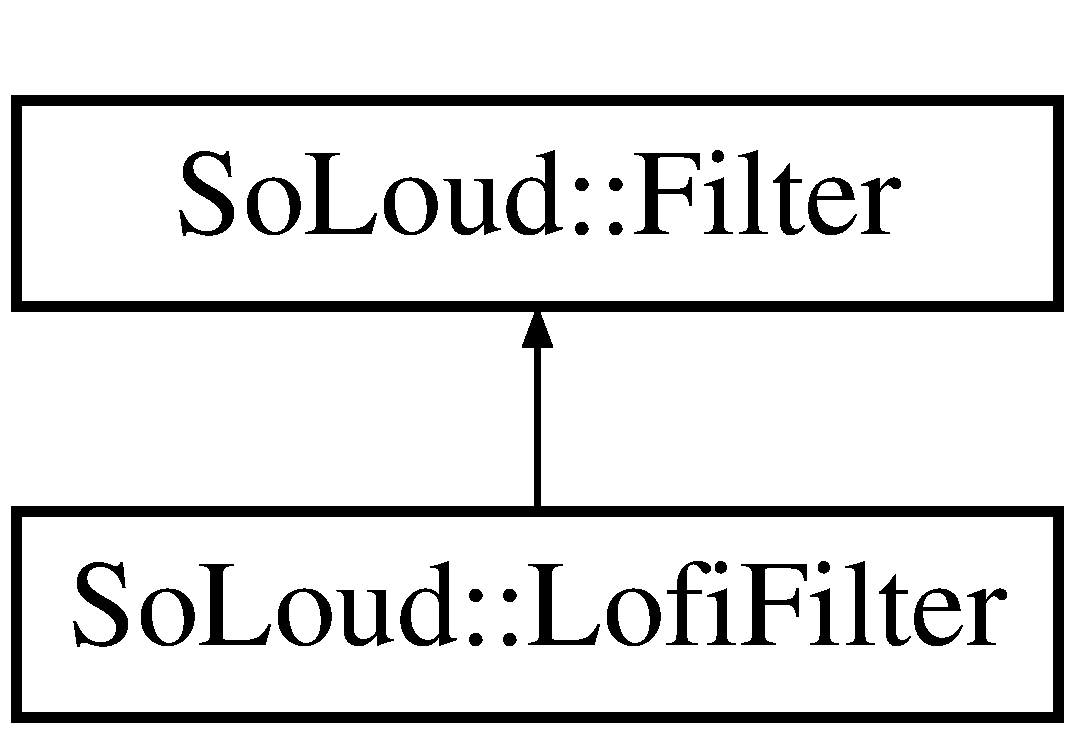
\includegraphics[height=2.000000cm]{class_so_loud_1_1_lofi_filter}
\end{center}
\end{figure}
\subsection*{Public Types}
\begin{DoxyCompactItemize}
\item 
\mbox{\Hypertarget{class_so_loud_1_1_lofi_filter_a628a6ed55f2e6b27b656c84deb1bf242}\label{class_so_loud_1_1_lofi_filter_a628a6ed55f2e6b27b656c84deb1bf242}} 
enum {\bfseries F\+I\+L\+T\+E\+R\+P\+A\+R\+A\+MS} \{ {\bfseries W\+ET}, 
{\bfseries S\+A\+M\+P\+L\+E\+R\+A\+TE}, 
{\bfseries B\+I\+T\+D\+E\+P\+TH}
 \}
\end{DoxyCompactItemize}
\subsection*{Public Member Functions}
\begin{DoxyCompactItemize}
\item 
\mbox{\Hypertarget{class_so_loud_1_1_lofi_filter_a0b7484ec8d440c34a787514a838d17f0}\label{class_so_loud_1_1_lofi_filter_a0b7484ec8d440c34a787514a838d17f0}} 
virtual \mbox{\hyperlink{class_so_loud_1_1_lofi_filter_instance}{Lofi\+Filter\+Instance}} $\ast$ {\bfseries create\+Instance} ()
\item 
\mbox{\Hypertarget{class_so_loud_1_1_lofi_filter_a08192a6e28088cf78518c684dba2e6eb}\label{class_so_loud_1_1_lofi_filter_a08192a6e28088cf78518c684dba2e6eb}} 
result {\bfseries set\+Params} (float a\+Sample\+Rate, float a\+Bitdepth)
\end{DoxyCompactItemize}
\subsection*{Public Attributes}
\begin{DoxyCompactItemize}
\item 
\mbox{\Hypertarget{class_so_loud_1_1_lofi_filter_afe20e30a72a4dc5b932a6a53fb09c3d0}\label{class_so_loud_1_1_lofi_filter_afe20e30a72a4dc5b932a6a53fb09c3d0}} 
float {\bfseries m\+Sample\+Rate}
\item 
\mbox{\Hypertarget{class_so_loud_1_1_lofi_filter_a6a2fe000f5f8e87031002de789f8fecc}\label{class_so_loud_1_1_lofi_filter_a6a2fe000f5f8e87031002de789f8fecc}} 
float {\bfseries m\+Bitdepth}
\end{DoxyCompactItemize}


The documentation for this class was generated from the following file\+:\begin{DoxyCompactItemize}
\item 
deps/\+E\+S\+A\+T/include/\+E\+S\+A\+T\+\_\+extra/soloud/soloud\+\_\+lofifilter.\+h\end{DoxyCompactItemize}

\hypertarget{class_so_loud_1_1_lofi_filter_instance}{}\section{So\+Loud\+:\+:Lofi\+Filter\+Instance Class Reference}
\label{class_so_loud_1_1_lofi_filter_instance}\index{So\+Loud\+::\+Lofi\+Filter\+Instance@{So\+Loud\+::\+Lofi\+Filter\+Instance}}
Inheritance diagram for So\+Loud\+:\+:Lofi\+Filter\+Instance\+:\begin{figure}[H]
\begin{center}
\leavevmode
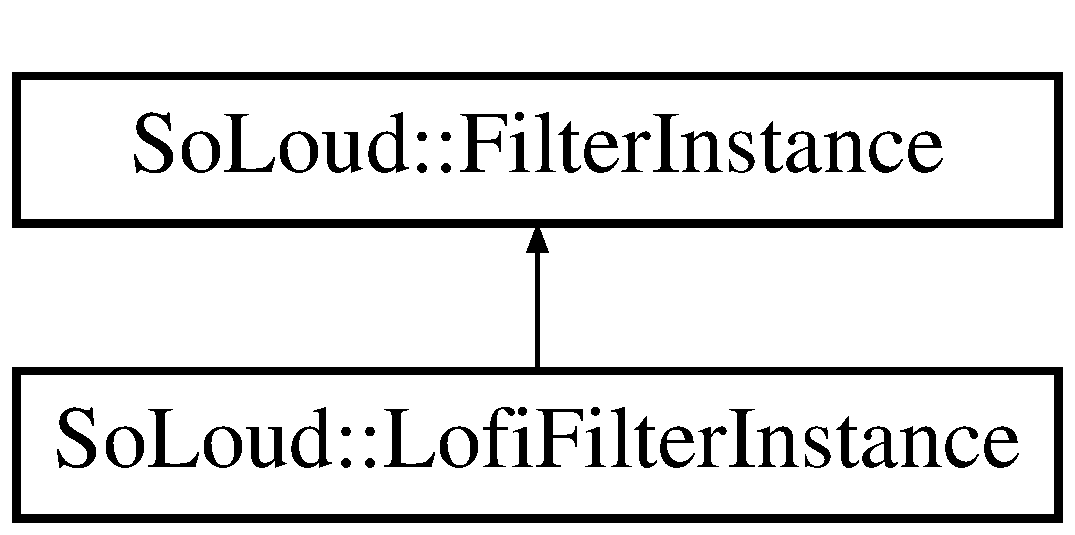
\includegraphics[height=2.000000cm]{class_so_loud_1_1_lofi_filter_instance}
\end{center}
\end{figure}
\subsection*{Public Member Functions}
\begin{DoxyCompactItemize}
\item 
\mbox{\Hypertarget{class_so_loud_1_1_lofi_filter_instance_a7fb089ce7b108786adc194865149c802}\label{class_so_loud_1_1_lofi_filter_instance_a7fb089ce7b108786adc194865149c802}} 
virtual void {\bfseries filter\+Channel} (float $\ast$a\+Buffer, unsigned int a\+Samples, float a\+Samplerate, time a\+Time, unsigned int a\+Channel, unsigned int a\+Channels)
\item 
\mbox{\Hypertarget{class_so_loud_1_1_lofi_filter_instance_afc69d044de0a65c130feca0c1001fa91}\label{class_so_loud_1_1_lofi_filter_instance_afc69d044de0a65c130feca0c1001fa91}} 
{\bfseries Lofi\+Filter\+Instance} (\mbox{\hyperlink{class_so_loud_1_1_lofi_filter}{Lofi\+Filter}} $\ast$a\+Parent)
\end{DoxyCompactItemize}
\subsection*{Additional Inherited Members}


The documentation for this class was generated from the following file\+:\begin{DoxyCompactItemize}
\item 
deps/\+E\+S\+A\+T/include/\+E\+S\+A\+T\+\_\+extra/soloud/soloud\+\_\+lofifilter.\+h\end{DoxyCompactItemize}

\hypertarget{class_map}{}\section{Map Class Reference}
\label{class_map}\index{Map@{Map}}


\mbox{\hyperlink{class_map}{Map}} class.  




{\ttfamily \#include $<$map.\+h$>$}

\subsection*{Public Member Functions}
\begin{DoxyCompactItemize}
\item 
\mbox{\hyperlink{class_map_a0f5ad0fd4563497b4214038cbca8b582}{Map}} ()
\begin{DoxyCompactList}\small\item\em \mbox{\hyperlink{class_map}{Map}} constructor. \end{DoxyCompactList}\item 
\mbox{\hyperlink{class_map_aa403fbe09394ccf39747588f5168e3b2}{$\sim$\+Map}} ()
\begin{DoxyCompactList}\small\item\em \mbox{\hyperlink{class_map}{Map}} destructor. \end{DoxyCompactList}\item 
bool \mbox{\hyperlink{class_map_a5b5c0989800c44a2db7a00bbf40c74a6}{is\+Valid\+Position}} (const float x, const float y) const
\begin{DoxyCompactList}\small\item\em checks if a position is a valid one in the map \end{DoxyCompactList}\item 
bool \mbox{\hyperlink{class_map_abc5d67212c69d40198e80f66e29cca7a}{is\+Occupied}} (const float x, const float y) const
\begin{DoxyCompactList}\small\item\em checks if a position is occupied in the map \end{DoxyCompactList}\item 
s16 \mbox{\hyperlink{class_map_a4070d04487b207e04c47b89b710c95a6}{load\+Map}} (const char $\ast$src, const char $\ast$\mbox{\hyperlink{class_map_ad2be03ca3f10013e1017c0ad4903641b}{background}})
\begin{DoxyCompactList}\small\item\em Loads the map. \end{DoxyCompactList}\item 
\mbox{\hyperlink{class_float2}{Float2}} \mbox{\hyperlink{class_map_ad27c66a5bfffc6aeb8c786b7edb19d22}{ratio}} () const
\begin{DoxyCompactList}\small\item\em returns the ratio between the original map and the collisions map \end{DoxyCompactList}\item 
E\+S\+A\+T\+::\+Sprite\+Handle \mbox{\hyperlink{class_map_ad2be03ca3f10013e1017c0ad4903641b}{background}} () const
\begin{DoxyCompactList}\small\item\em returns the image of the original map \end{DoxyCompactList}\end{DoxyCompactItemize}


\subsection{Detailed Description}
\mbox{\hyperlink{class_map}{Map}} class. 

Class in charge of storing the background representation of the map and it\textquotesingle{}s collision data 

\subsection{Constructor \& Destructor Documentation}
\mbox{\Hypertarget{class_map_a0f5ad0fd4563497b4214038cbca8b582}\label{class_map_a0f5ad0fd4563497b4214038cbca8b582}} 
\index{Map@{Map}!Map@{Map}}
\index{Map@{Map}!Map@{Map}}
\subsubsection{\texorpdfstring{Map()}{Map()}}
{\footnotesize\ttfamily Map\+::\+Map (\begin{DoxyParamCaption}{ }\end{DoxyParamCaption})}



\mbox{\hyperlink{class_map}{Map}} constructor. 

Default \mbox{\hyperlink{class_map}{Map}} constructor

\begin{DoxyReturn}{Returns}
$\ast$\+Map 
\end{DoxyReturn}
\mbox{\Hypertarget{class_map_aa403fbe09394ccf39747588f5168e3b2}\label{class_map_aa403fbe09394ccf39747588f5168e3b2}} 
\index{Map@{Map}!````~Map@{$\sim$\+Map}}
\index{````~Map@{$\sim$\+Map}!Map@{Map}}
\subsubsection{\texorpdfstring{$\sim$\+Map()}{~Map()}}
{\footnotesize\ttfamily Map\+::$\sim$\+Map (\begin{DoxyParamCaption}{ }\end{DoxyParamCaption})}



\mbox{\hyperlink{class_map}{Map}} destructor. 

Default \mbox{\hyperlink{class_map}{Map}} destructor

\begin{DoxyReturn}{Returns}
$\ast$\+Map 
\end{DoxyReturn}


\subsection{Member Function Documentation}
\mbox{\Hypertarget{class_map_ad2be03ca3f10013e1017c0ad4903641b}\label{class_map_ad2be03ca3f10013e1017c0ad4903641b}} 
\index{Map@{Map}!background@{background}}
\index{background@{background}!Map@{Map}}
\subsubsection{\texorpdfstring{background()}{background()}}
{\footnotesize\ttfamily E\+S\+A\+T\+::\+Sprite\+Handle Map\+::background (\begin{DoxyParamCaption}{ }\end{DoxyParamCaption}) const}



returns the image of the original map 

Returns the image of the original map

\begin{DoxyReturn}{Returns}
Sprite\+Handle image of the background 
\end{DoxyReturn}
\mbox{\Hypertarget{class_map_abc5d67212c69d40198e80f66e29cca7a}\label{class_map_abc5d67212c69d40198e80f66e29cca7a}} 
\index{Map@{Map}!is\+Occupied@{is\+Occupied}}
\index{is\+Occupied@{is\+Occupied}!Map@{Map}}
\subsubsection{\texorpdfstring{is\+Occupied()}{isOccupied()}}
{\footnotesize\ttfamily bool Map\+::is\+Occupied (\begin{DoxyParamCaption}\item[{const float}]{x,  }\item[{const float}]{y }\end{DoxyParamCaption}) const}



checks if a position is occupied in the map 

Checks if a position is occupied in the map


\begin{DoxyParams}{Parameters}
{\em x} & x coordinate of the position we want to check \\
\hline
{\em y} & y coordinate of the position we want to check \\
\hline
\end{DoxyParams}
\begin{DoxyReturn}{Returns}
bool true if it is valid false otherwise 
\end{DoxyReturn}
\mbox{\Hypertarget{class_map_a5b5c0989800c44a2db7a00bbf40c74a6}\label{class_map_a5b5c0989800c44a2db7a00bbf40c74a6}} 
\index{Map@{Map}!is\+Valid\+Position@{is\+Valid\+Position}}
\index{is\+Valid\+Position@{is\+Valid\+Position}!Map@{Map}}
\subsubsection{\texorpdfstring{is\+Valid\+Position()}{isValidPosition()}}
{\footnotesize\ttfamily bool Map\+::is\+Valid\+Position (\begin{DoxyParamCaption}\item[{const float}]{x,  }\item[{const float}]{y }\end{DoxyParamCaption}) const}



checks if a position is a valid one in the map 

Checks if a position is a valid one in the map


\begin{DoxyParams}{Parameters}
{\em x} & x coordinate of the position we want to check \\
\hline
{\em y} & y coordinate of the position we want to check \\
\hline
\end{DoxyParams}
\begin{DoxyReturn}{Returns}
bool true if it is valid false otherwise 
\end{DoxyReturn}
\mbox{\Hypertarget{class_map_a4070d04487b207e04c47b89b710c95a6}\label{class_map_a4070d04487b207e04c47b89b710c95a6}} 
\index{Map@{Map}!load\+Map@{load\+Map}}
\index{load\+Map@{load\+Map}!Map@{Map}}
\subsubsection{\texorpdfstring{load\+Map()}{loadMap()}}
{\footnotesize\ttfamily s16 Map\+::load\+Map (\begin{DoxyParamCaption}\item[{const char $\ast$}]{src,  }\item[{const char $\ast$}]{background }\end{DoxyParamCaption})}



Loads the map. 

Tries to load a map with an image source for the background and an image source for the collisions ( white = free, black = occupied). If another map was already loaded it will be freed. The possible results of this operation are\+: k\+Error\+Code\+\_\+\+Invalid\+Pointer -\/$>$ The source or the background were nullptr k\+Error\+Code\+\_\+\+Memory -\/$>$ The program was unable of allocating memory k\+Error\+Code\+\_\+\+Ok -\/$>$ Everything went fine


\begin{DoxyParams}{Parameters}
{\em src} & x coordinate of the position we want to check \\
\hline
{\em background} & y coordinate of the position we want to check \\
\hline
\end{DoxyParams}
\begin{DoxyReturn}{Returns}
status of the operation 
\end{DoxyReturn}
\mbox{\Hypertarget{class_map_ad27c66a5bfffc6aeb8c786b7edb19d22}\label{class_map_ad27c66a5bfffc6aeb8c786b7edb19d22}} 
\index{Map@{Map}!ratio@{ratio}}
\index{ratio@{ratio}!Map@{Map}}
\subsubsection{\texorpdfstring{ratio()}{ratio()}}
{\footnotesize\ttfamily \mbox{\hyperlink{class_float2}{Float2}} Map\+::ratio (\begin{DoxyParamCaption}{ }\end{DoxyParamCaption}) const}



returns the ratio between the original map and the collisions map 

Returns the ratio between the original map and the collisions map

\begin{DoxyReturn}{Returns}
\mbox{\hyperlink{class_float2}{Float2}} ratio 
\end{DoxyReturn}


The documentation for this class was generated from the following files\+:\begin{DoxyCompactItemize}
\item 
include/map.\+h\item 
src/map.\+cc\end{DoxyCompactItemize}

\hypertarget{struct_e_s_a_t_1_1_mat3}{}\section{E\+S\+AT\+:\+:Mat3 Struct Reference}
\label{struct_e_s_a_t_1_1_mat3}\index{E\+S\+A\+T\+::\+Mat3@{E\+S\+A\+T\+::\+Mat3}}
\subsection*{Public Attributes}
\begin{DoxyCompactItemize}
\item 
\mbox{\Hypertarget{struct_e_s_a_t_1_1_mat3_a5f4428530a273807e3f597903a2d8fe9}\label{struct_e_s_a_t_1_1_mat3_a5f4428530a273807e3f597903a2d8fe9}} 
float {\bfseries d} \mbox{[}9\mbox{]}
\end{DoxyCompactItemize}


The documentation for this struct was generated from the following file\+:\begin{DoxyCompactItemize}
\item 
deps/\+E\+S\+A\+T/include/\+E\+S\+A\+T/math.\+h\end{DoxyCompactItemize}

\hypertarget{struct_e_s_a_t_1_1_mat4}{}\section{E\+S\+AT\+:\+:Mat4 Struct Reference}
\label{struct_e_s_a_t_1_1_mat4}\index{E\+S\+A\+T\+::\+Mat4@{E\+S\+A\+T\+::\+Mat4}}
\subsection*{Public Attributes}
\begin{DoxyCompactItemize}
\item 
\mbox{\Hypertarget{struct_e_s_a_t_1_1_mat4_ab4dafd527900868b3a5dcc27ca583755}\label{struct_e_s_a_t_1_1_mat4_ab4dafd527900868b3a5dcc27ca583755}} 
float {\bfseries d} \mbox{[}16\mbox{]}
\end{DoxyCompactItemize}


The documentation for this struct was generated from the following file\+:\begin{DoxyCompactItemize}
\item 
deps/\+E\+S\+A\+T/include/\+E\+S\+A\+T/math.\+h\end{DoxyCompactItemize}

\hypertarget{structtinyobj_1_1material__t}{}\section{tinyobj\+:\+:material\+\_\+t Struct Reference}
\label{structtinyobj_1_1material__t}\index{tinyobj\+::material\+\_\+t@{tinyobj\+::material\+\_\+t}}
\subsection*{Public Attributes}
\begin{DoxyCompactItemize}
\item 
\mbox{\Hypertarget{structtinyobj_1_1material__t_a41fde82dd0ec383b1d4ee258c4e4a1b9}\label{structtinyobj_1_1material__t_a41fde82dd0ec383b1d4ee258c4e4a1b9}} 
std\+::string {\bfseries name}
\item 
\mbox{\Hypertarget{structtinyobj_1_1material__t_a43b73b4858f8901eea238e007c8719ce}\label{structtinyobj_1_1material__t_a43b73b4858f8901eea238e007c8719ce}} 
float {\bfseries ambient} \mbox{[}3\mbox{]}
\item 
\mbox{\Hypertarget{structtinyobj_1_1material__t_a6ca52b575604328ad4d5674b2891a780}\label{structtinyobj_1_1material__t_a6ca52b575604328ad4d5674b2891a780}} 
float {\bfseries diffuse} \mbox{[}3\mbox{]}
\item 
\mbox{\Hypertarget{structtinyobj_1_1material__t_a7bbad62eae583d5c381909f1f4f76471}\label{structtinyobj_1_1material__t_a7bbad62eae583d5c381909f1f4f76471}} 
float {\bfseries specular} \mbox{[}3\mbox{]}
\item 
\mbox{\Hypertarget{structtinyobj_1_1material__t_a40e7cf9bc5c2cf9048152d39be6b82d7}\label{structtinyobj_1_1material__t_a40e7cf9bc5c2cf9048152d39be6b82d7}} 
float {\bfseries transmittance} \mbox{[}3\mbox{]}
\item 
\mbox{\Hypertarget{structtinyobj_1_1material__t_ab84b63eb4a936b6fba7392cdcea6d6f6}\label{structtinyobj_1_1material__t_ab84b63eb4a936b6fba7392cdcea6d6f6}} 
float {\bfseries emission} \mbox{[}3\mbox{]}
\item 
\mbox{\Hypertarget{structtinyobj_1_1material__t_a4f893e510fd30f63c687a8ad53000d15}\label{structtinyobj_1_1material__t_a4f893e510fd30f63c687a8ad53000d15}} 
float {\bfseries shininess}
\item 
\mbox{\Hypertarget{structtinyobj_1_1material__t_aaa7d5495ba26b249e2ea3c368b505b56}\label{structtinyobj_1_1material__t_aaa7d5495ba26b249e2ea3c368b505b56}} 
float {\bfseries ior}
\item 
\mbox{\Hypertarget{structtinyobj_1_1material__t_ac7dfb767305c4225c5b3a964acb9498d}\label{structtinyobj_1_1material__t_ac7dfb767305c4225c5b3a964acb9498d}} 
float {\bfseries dissolve}
\item 
\mbox{\Hypertarget{structtinyobj_1_1material__t_af846245315bd70c1a4f815dfdd6b80cc}\label{structtinyobj_1_1material__t_af846245315bd70c1a4f815dfdd6b80cc}} 
int {\bfseries illum}
\item 
\mbox{\Hypertarget{structtinyobj_1_1material__t_a6b1814d1066609178c81d2a4f7b34bd8}\label{structtinyobj_1_1material__t_a6b1814d1066609178c81d2a4f7b34bd8}} 
int {\bfseries dummy}
\item 
\mbox{\Hypertarget{structtinyobj_1_1material__t_ae988eed637f368374becbb672798a45e}\label{structtinyobj_1_1material__t_ae988eed637f368374becbb672798a45e}} 
std\+::string {\bfseries ambient\+\_\+texname}
\item 
\mbox{\Hypertarget{structtinyobj_1_1material__t_ad7f71a301a261fca07d2e50edccc792d}\label{structtinyobj_1_1material__t_ad7f71a301a261fca07d2e50edccc792d}} 
std\+::string {\bfseries diffuse\+\_\+texname}
\item 
\mbox{\Hypertarget{structtinyobj_1_1material__t_aed8c38d64472ba0db5186dba800b1b34}\label{structtinyobj_1_1material__t_aed8c38d64472ba0db5186dba800b1b34}} 
std\+::string {\bfseries specular\+\_\+texname}
\item 
\mbox{\Hypertarget{structtinyobj_1_1material__t_a5c0e981297646f1fc1aeba616692c41b}\label{structtinyobj_1_1material__t_a5c0e981297646f1fc1aeba616692c41b}} 
std\+::string {\bfseries specular\+\_\+highlight\+\_\+texname}
\item 
\mbox{\Hypertarget{structtinyobj_1_1material__t_aceb73086232f1cdd82f956fe8c6efcfb}\label{structtinyobj_1_1material__t_aceb73086232f1cdd82f956fe8c6efcfb}} 
std\+::string {\bfseries bump\+\_\+texname}
\item 
\mbox{\Hypertarget{structtinyobj_1_1material__t_ab69842db3e67cc7d4dcd8bfe02590f92}\label{structtinyobj_1_1material__t_ab69842db3e67cc7d4dcd8bfe02590f92}} 
std\+::string {\bfseries displacement\+\_\+texname}
\item 
\mbox{\Hypertarget{structtinyobj_1_1material__t_a1b0225fd76de506f089fdedbf2c66dec}\label{structtinyobj_1_1material__t_a1b0225fd76de506f089fdedbf2c66dec}} 
std\+::string {\bfseries alpha\+\_\+texname}
\item 
\mbox{\Hypertarget{structtinyobj_1_1material__t_a18b700227c94d410ed1aa550c7fa9226}\label{structtinyobj_1_1material__t_a18b700227c94d410ed1aa550c7fa9226}} 
std\+::map$<$ std\+::string, std\+::string $>$ {\bfseries unknown\+\_\+parameter}
\end{DoxyCompactItemize}


The documentation for this struct was generated from the following file\+:\begin{DoxyCompactItemize}
\item 
deps/\+E\+S\+A\+T/include/\+E\+S\+A\+T\+\_\+extra/tiny\+\_\+obj\+\_\+loader.\+h\end{DoxyCompactItemize}

\hypertarget{classtinyobj_1_1_material_file_reader}{}\section{tinyobj\+:\+:Material\+File\+Reader Class Reference}
\label{classtinyobj_1_1_material_file_reader}\index{tinyobj\+::\+Material\+File\+Reader@{tinyobj\+::\+Material\+File\+Reader}}
Inheritance diagram for tinyobj\+:\+:Material\+File\+Reader\+:\begin{figure}[H]
\begin{center}
\leavevmode
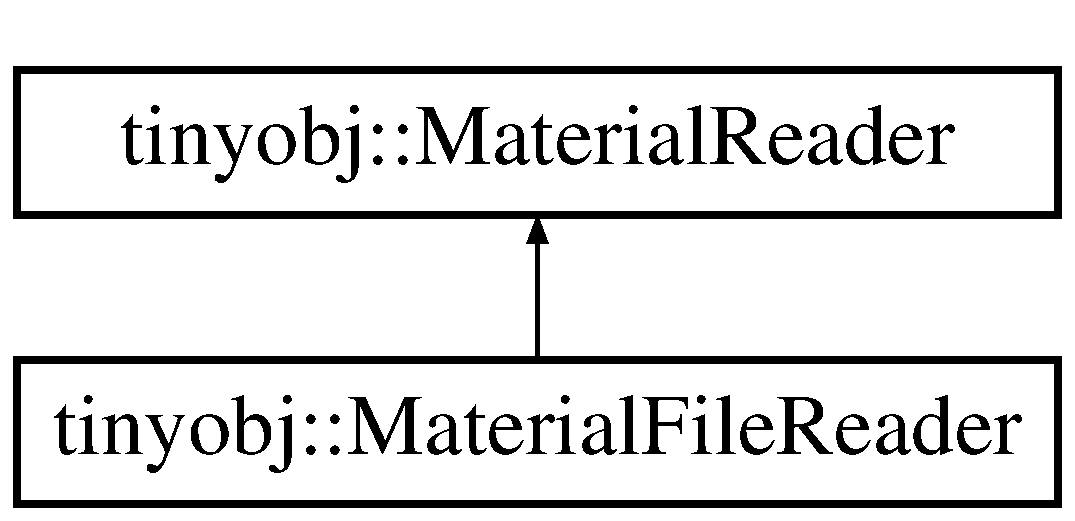
\includegraphics[height=2.000000cm]{classtinyobj_1_1_material_file_reader}
\end{center}
\end{figure}
\subsection*{Public Member Functions}
\begin{DoxyCompactItemize}
\item 
\mbox{\Hypertarget{classtinyobj_1_1_material_file_reader_a824d0100284310fe213d86ad443cc575}\label{classtinyobj_1_1_material_file_reader_a824d0100284310fe213d86ad443cc575}} 
{\bfseries Material\+File\+Reader} (const std\+::string \&mtl\+\_\+basepath)
\item 
\mbox{\Hypertarget{classtinyobj_1_1_material_file_reader_a0b9f3231d766fe14d6a20ea645447a74}\label{classtinyobj_1_1_material_file_reader_a0b9f3231d766fe14d6a20ea645447a74}} 
virtual bool {\bfseries operator()} (const std\+::string \&mat\+Id, std\+::vector$<$ \mbox{\hyperlink{structtinyobj_1_1material__t}{material\+\_\+t}} $>$ \&materials, std\+::map$<$ std\+::string, int $>$ \&mat\+Map, std\+::string \&err)
\end{DoxyCompactItemize}


The documentation for this class was generated from the following file\+:\begin{DoxyCompactItemize}
\item 
deps/\+E\+S\+A\+T/include/\+E\+S\+A\+T\+\_\+extra/tiny\+\_\+obj\+\_\+loader.\+h\end{DoxyCompactItemize}

\hypertarget{classtinyobj_1_1_material_reader}{}\section{tinyobj\+:\+:Material\+Reader Class Reference}
\label{classtinyobj_1_1_material_reader}\index{tinyobj\+::\+Material\+Reader@{tinyobj\+::\+Material\+Reader}}
Inheritance diagram for tinyobj\+:\+:Material\+Reader\+:\begin{figure}[H]
\begin{center}
\leavevmode
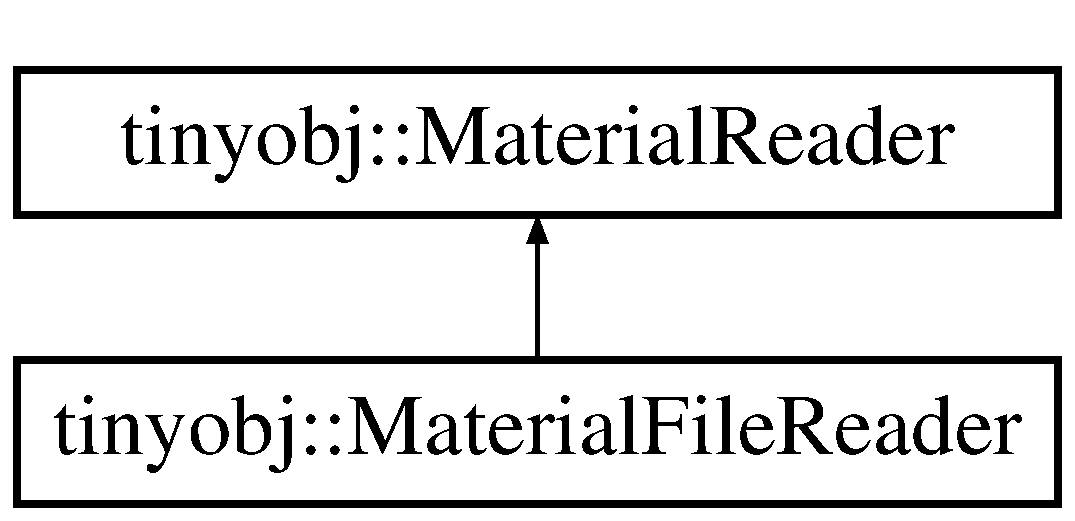
\includegraphics[height=2.000000cm]{classtinyobj_1_1_material_reader}
\end{center}
\end{figure}
\subsection*{Public Member Functions}
\begin{DoxyCompactItemize}
\item 
\mbox{\Hypertarget{classtinyobj_1_1_material_reader_afa193c78cea3a3618808165ba19697e0}\label{classtinyobj_1_1_material_reader_afa193c78cea3a3618808165ba19697e0}} 
virtual bool {\bfseries operator()} (const std\+::string \&mat\+Id, std\+::vector$<$ \mbox{\hyperlink{structtinyobj_1_1material__t}{material\+\_\+t}} $>$ \&materials, std\+::map$<$ std\+::string, int $>$ \&mat\+Map, std\+::string \&err)=0
\end{DoxyCompactItemize}


The documentation for this class was generated from the following file\+:\begin{DoxyCompactItemize}
\item 
deps/\+E\+S\+A\+T/include/\+E\+S\+A\+T\+\_\+extra/tiny\+\_\+obj\+\_\+loader.\+h\end{DoxyCompactItemize}

\hypertarget{class_so_loud_1_1_memory_file}{}\section{So\+Loud\+:\+:Memory\+File Class Reference}
\label{class_so_loud_1_1_memory_file}\index{So\+Loud\+::\+Memory\+File@{So\+Loud\+::\+Memory\+File}}
Inheritance diagram for So\+Loud\+:\+:Memory\+File\+:\begin{figure}[H]
\begin{center}
\leavevmode
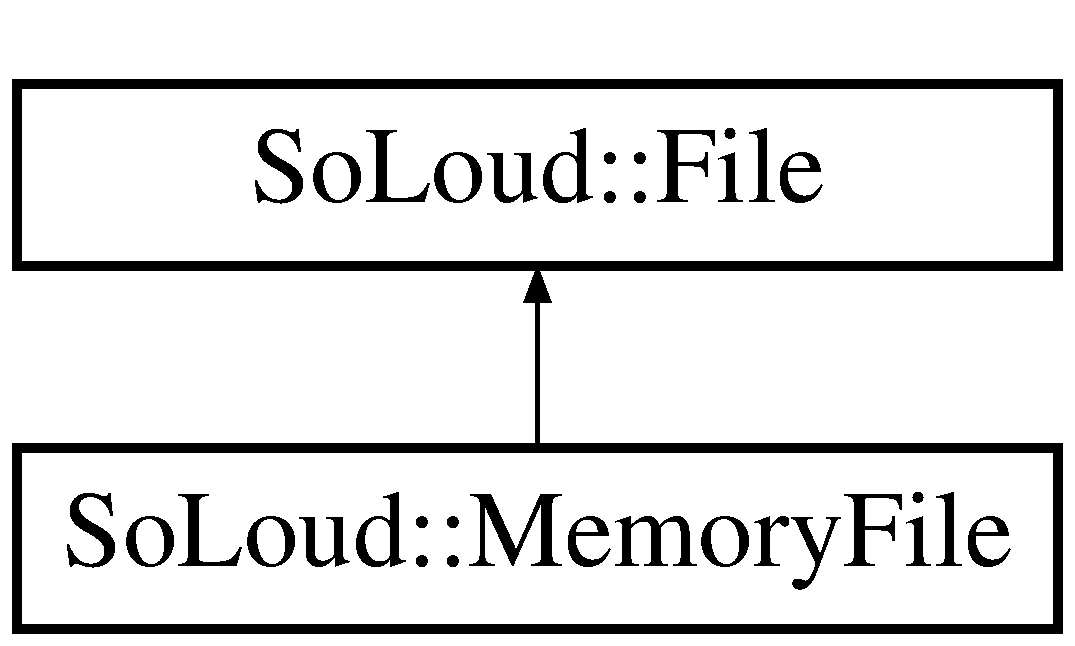
\includegraphics[height=2.000000cm]{class_so_loud_1_1_memory_file}
\end{center}
\end{figure}
\subsection*{Public Member Functions}
\begin{DoxyCompactItemize}
\item 
\mbox{\Hypertarget{class_so_loud_1_1_memory_file_acfe99485f35ab6c86ee803a7d8264ac5}\label{class_so_loud_1_1_memory_file_acfe99485f35ab6c86ee803a7d8264ac5}} 
virtual int {\bfseries eof} ()
\item 
\mbox{\Hypertarget{class_so_loud_1_1_memory_file_ad536746b8182f14f5201e56a35c23d69}\label{class_so_loud_1_1_memory_file_ad536746b8182f14f5201e56a35c23d69}} 
virtual unsigned int {\bfseries read} (unsigned char $\ast$a\+Dst, unsigned int a\+Bytes)
\item 
\mbox{\Hypertarget{class_so_loud_1_1_memory_file_a6008eda4f47eb0d9d1f62ffb48b42f36}\label{class_so_loud_1_1_memory_file_a6008eda4f47eb0d9d1f62ffb48b42f36}} 
virtual unsigned int {\bfseries length} ()
\item 
\mbox{\Hypertarget{class_so_loud_1_1_memory_file_a9f381c66f4803d69fabc9a88dd89c51e}\label{class_so_loud_1_1_memory_file_a9f381c66f4803d69fabc9a88dd89c51e}} 
virtual void {\bfseries seek} (int a\+Offset)
\item 
\mbox{\Hypertarget{class_so_loud_1_1_memory_file_ac698163e644dddb838ea01152c1583a3}\label{class_so_loud_1_1_memory_file_ac698163e644dddb838ea01152c1583a3}} 
virtual unsigned int {\bfseries pos} ()
\item 
\mbox{\Hypertarget{class_so_loud_1_1_memory_file_adce1b3d03cd39ed2fd6ac55c016816c4}\label{class_so_loud_1_1_memory_file_adce1b3d03cd39ed2fd6ac55c016816c4}} 
virtual unsigned char $\ast$ {\bfseries get\+Mem\+Ptr} ()
\item 
\mbox{\Hypertarget{class_so_loud_1_1_memory_file_ae7cb1c1a67e3b7c823f476b020c13d65}\label{class_so_loud_1_1_memory_file_ae7cb1c1a67e3b7c823f476b020c13d65}} 
result {\bfseries open\+Mem} (unsigned char $\ast$a\+Data, unsigned int a\+Data\+Length, bool a\+Copy=false, bool a\+Take\+Ownership=true)
\item 
\mbox{\Hypertarget{class_so_loud_1_1_memory_file_ad5f92cd7d93255151b817169ec9ab9b6}\label{class_so_loud_1_1_memory_file_ad5f92cd7d93255151b817169ec9ab9b6}} 
result {\bfseries open\+To\+Mem} (const char $\ast$a\+Filename)
\item 
\mbox{\Hypertarget{class_so_loud_1_1_memory_file_a7cb55217fc03da894d3463f7577f45dd}\label{class_so_loud_1_1_memory_file_a7cb55217fc03da894d3463f7577f45dd}} 
result {\bfseries open\+File\+To\+Mem} (\mbox{\hyperlink{class_so_loud_1_1_file}{File}} $\ast$a\+File)
\end{DoxyCompactItemize}
\subsection*{Public Attributes}
\begin{DoxyCompactItemize}
\item 
\mbox{\Hypertarget{class_so_loud_1_1_memory_file_aff89e6baa16c1ca90c97aa3dbd3d20f9}\label{class_so_loud_1_1_memory_file_aff89e6baa16c1ca90c97aa3dbd3d20f9}} 
unsigned char $\ast$ {\bfseries m\+Data\+Ptr}
\item 
\mbox{\Hypertarget{class_so_loud_1_1_memory_file_ab407b1a28480fb1e7526f4fbaaeeafd0}\label{class_so_loud_1_1_memory_file_ab407b1a28480fb1e7526f4fbaaeeafd0}} 
unsigned int {\bfseries m\+Data\+Length}
\item 
\mbox{\Hypertarget{class_so_loud_1_1_memory_file_a20c583c361b6564bea362c6a9a1e7682}\label{class_so_loud_1_1_memory_file_a20c583c361b6564bea362c6a9a1e7682}} 
unsigned int {\bfseries m\+Offset}
\item 
\mbox{\Hypertarget{class_so_loud_1_1_memory_file_a2ee4bfc90fa42f79f78f3663c446b6db}\label{class_so_loud_1_1_memory_file_a2ee4bfc90fa42f79f78f3663c446b6db}} 
bool {\bfseries m\+Data\+Owned}
\end{DoxyCompactItemize}


The documentation for this class was generated from the following file\+:\begin{DoxyCompactItemize}
\item 
deps/\+E\+S\+A\+T/include/\+E\+S\+A\+T\+\_\+extra/soloud/soloud\+\_\+file.\+h\end{DoxyCompactItemize}

\hypertarget{structtinyobj_1_1mesh__t}{}\section{tinyobj\+:\+:mesh\+\_\+t Struct Reference}
\label{structtinyobj_1_1mesh__t}\index{tinyobj\+::mesh\+\_\+t@{tinyobj\+::mesh\+\_\+t}}
\subsection*{Public Attributes}
\begin{DoxyCompactItemize}
\item 
\mbox{\Hypertarget{structtinyobj_1_1mesh__t_a3014a27913256384aa283345b69ff2ec}\label{structtinyobj_1_1mesh__t_a3014a27913256384aa283345b69ff2ec}} 
std\+::vector$<$ float $>$ {\bfseries positions}
\item 
\mbox{\Hypertarget{structtinyobj_1_1mesh__t_a28c2f7eb3114e6ed82a5b7326a4e7a1c}\label{structtinyobj_1_1mesh__t_a28c2f7eb3114e6ed82a5b7326a4e7a1c}} 
std\+::vector$<$ float $>$ {\bfseries normals}
\item 
\mbox{\Hypertarget{structtinyobj_1_1mesh__t_a0fc485afc76bcd7e147b22285d7d6575}\label{structtinyobj_1_1mesh__t_a0fc485afc76bcd7e147b22285d7d6575}} 
std\+::vector$<$ float $>$ {\bfseries texcoords}
\item 
\mbox{\Hypertarget{structtinyobj_1_1mesh__t_aa0a07f40559a650e6917c506d78e298a}\label{structtinyobj_1_1mesh__t_aa0a07f40559a650e6917c506d78e298a}} 
std\+::vector$<$ unsigned int $>$ {\bfseries indices}
\item 
\mbox{\Hypertarget{structtinyobj_1_1mesh__t_aa4858f9a5941c179f76d272b389af954}\label{structtinyobj_1_1mesh__t_aa4858f9a5941c179f76d272b389af954}} 
std\+::vector$<$ unsigned char $>$ {\bfseries num\+\_\+vertices}
\item 
\mbox{\Hypertarget{structtinyobj_1_1mesh__t_a57b2f12dfa3fd620b25babcd3a09ec6b}\label{structtinyobj_1_1mesh__t_a57b2f12dfa3fd620b25babcd3a09ec6b}} 
std\+::vector$<$ int $>$ {\bfseries material\+\_\+ids}
\item 
\mbox{\Hypertarget{structtinyobj_1_1mesh__t_a60f51d3802c11e2bf269530e0337fc63}\label{structtinyobj_1_1mesh__t_a60f51d3802c11e2bf269530e0337fc63}} 
std\+::vector$<$ \mbox{\hyperlink{structtinyobj_1_1tag__t}{tag\+\_\+t}} $>$ {\bfseries tags}
\end{DoxyCompactItemize}


The documentation for this struct was generated from the following file\+:\begin{DoxyCompactItemize}
\item 
deps/\+E\+S\+A\+T/include/\+E\+S\+A\+T\+\_\+extra/tiny\+\_\+obj\+\_\+loader.\+h\end{DoxyCompactItemize}

\hypertarget{struct_e_s_a_t_1_1_message}{}\section{E\+S\+AT\+:\+:Message Struct Reference}
\label{struct_e_s_a_t_1_1_message}\index{E\+S\+A\+T\+::\+Message@{E\+S\+A\+T\+::\+Message}}
\subsection*{Public Attributes}
\begin{DoxyCompactItemize}
\item 
\mbox{\Hypertarget{struct_e_s_a_t_1_1_message_a8916a9cbc44e7451b3dd310db2135f8f}\label{struct_e_s_a_t_1_1_message_a8916a9cbc44e7451b3dd310db2135f8f}} 
const void $\ast$ {\bfseries mem}
\item 
\mbox{\Hypertarget{struct_e_s_a_t_1_1_message_a68299efa83e982ab5409e78211f6b69d}\label{struct_e_s_a_t_1_1_message_a68299efa83e982ab5409e78211f6b69d}} 
size\+\_\+t {\bfseries size}
\end{DoxyCompactItemize}


The documentation for this struct was generated from the following file\+:\begin{DoxyCompactItemize}
\item 
deps/\+E\+S\+A\+T/include/\+E\+S\+A\+T/network.\+h\end{DoxyCompactItemize}

\hypertarget{class_so_loud_1_1_modplug}{}\section{So\+Loud\+:\+:Modplug Class Reference}
\label{class_so_loud_1_1_modplug}\index{So\+Loud\+::\+Modplug@{So\+Loud\+::\+Modplug}}
Inheritance diagram for So\+Loud\+:\+:Modplug\+:\begin{figure}[H]
\begin{center}
\leavevmode
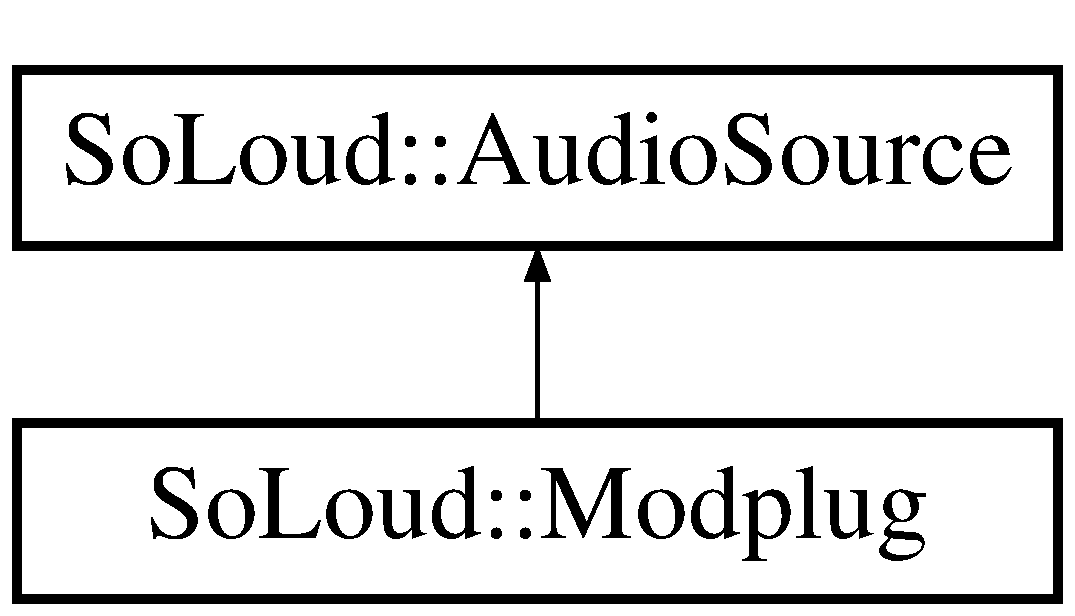
\includegraphics[height=2.000000cm]{class_so_loud_1_1_modplug}
\end{center}
\end{figure}
\subsection*{Public Member Functions}
\begin{DoxyCompactItemize}
\item 
\mbox{\Hypertarget{class_so_loud_1_1_modplug_a486803f7e617f4c6eafa9f96d87b7128}\label{class_so_loud_1_1_modplug_a486803f7e617f4c6eafa9f96d87b7128}} 
result {\bfseries load} (const char $\ast$a\+Filename)
\item 
\mbox{\Hypertarget{class_so_loud_1_1_modplug_a95562234f05f40ae86323e3b841321a3}\label{class_so_loud_1_1_modplug_a95562234f05f40ae86323e3b841321a3}} 
result {\bfseries load\+Mem} (unsigned char $\ast$a\+Mem, unsigned int a\+Length, bool a\+Copy=false, bool a\+Take\+Ownership=true)
\item 
\mbox{\Hypertarget{class_so_loud_1_1_modplug_ac5c4205c9d33aef5bf79e0d1c2ad0596}\label{class_so_loud_1_1_modplug_ac5c4205c9d33aef5bf79e0d1c2ad0596}} 
result {\bfseries load\+File} (\mbox{\hyperlink{class_so_loud_1_1_file}{File}} $\ast$a\+File)
\item 
\mbox{\Hypertarget{class_so_loud_1_1_modplug_aa39d19fa443edc644f0863469158d28d}\label{class_so_loud_1_1_modplug_aa39d19fa443edc644f0863469158d28d}} 
virtual \mbox{\hyperlink{class_so_loud_1_1_audio_source_instance}{Audio\+Source\+Instance}} $\ast$ {\bfseries create\+Instance} ()
\end{DoxyCompactItemize}
\subsection*{Public Attributes}
\begin{DoxyCompactItemize}
\item 
\mbox{\Hypertarget{class_so_loud_1_1_modplug_a4f810eeb4cd1a284f98bbb76cecfbe9f}\label{class_so_loud_1_1_modplug_a4f810eeb4cd1a284f98bbb76cecfbe9f}} 
char $\ast$ {\bfseries m\+Data}
\item 
\mbox{\Hypertarget{class_so_loud_1_1_modplug_a4a009a0351020a5cd02a7552310bdc32}\label{class_so_loud_1_1_modplug_a4a009a0351020a5cd02a7552310bdc32}} 
unsigned int {\bfseries m\+Data\+Len}
\end{DoxyCompactItemize}
\subsection*{Additional Inherited Members}


The documentation for this class was generated from the following file\+:\begin{DoxyCompactItemize}
\item 
deps/\+E\+S\+A\+T/include/\+E\+S\+A\+T\+\_\+extra/soloud/soloud\+\_\+modplug.\+h\end{DoxyCompactItemize}

\hypertarget{class_so_loud_1_1_modplug_instance}{}\section{So\+Loud\+:\+:Modplug\+Instance Class Reference}
\label{class_so_loud_1_1_modplug_instance}\index{So\+Loud\+::\+Modplug\+Instance@{So\+Loud\+::\+Modplug\+Instance}}
Inheritance diagram for So\+Loud\+:\+:Modplug\+Instance\+:\begin{figure}[H]
\begin{center}
\leavevmode
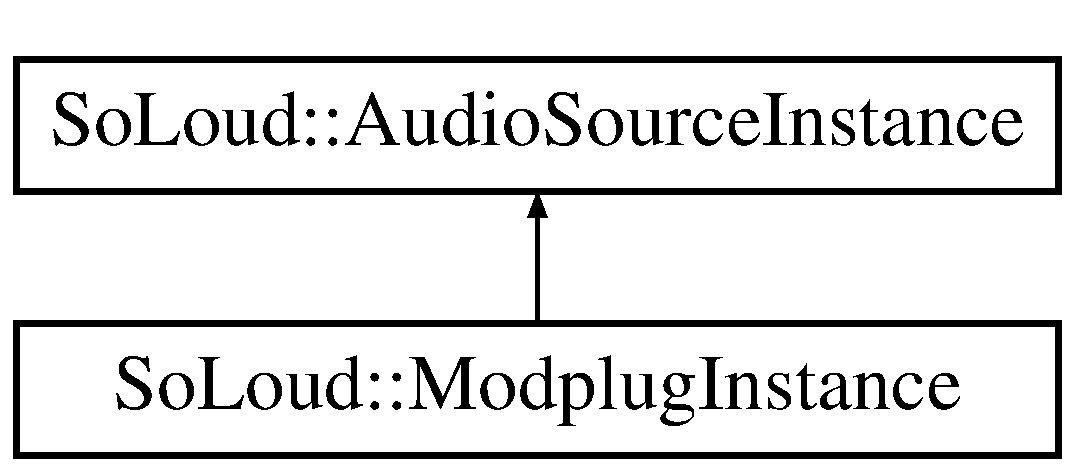
\includegraphics[height=2.000000cm]{class_so_loud_1_1_modplug_instance}
\end{center}
\end{figure}
\subsection*{Public Member Functions}
\begin{DoxyCompactItemize}
\item 
\mbox{\Hypertarget{class_so_loud_1_1_modplug_instance_a3f4cfdc6ca8cd7cd7bea503bf6acc4c6}\label{class_so_loud_1_1_modplug_instance_a3f4cfdc6ca8cd7cd7bea503bf6acc4c6}} 
{\bfseries Modplug\+Instance} (\mbox{\hyperlink{class_so_loud_1_1_modplug}{Modplug}} $\ast$a\+Parent)
\item 
\mbox{\Hypertarget{class_so_loud_1_1_modplug_instance_ab8deab09096e344e6876ec9e7b124a09}\label{class_so_loud_1_1_modplug_instance_ab8deab09096e344e6876ec9e7b124a09}} 
virtual void {\bfseries get\+Audio} (float $\ast$a\+Buffer, unsigned int a\+Samples)
\item 
\mbox{\Hypertarget{class_so_loud_1_1_modplug_instance_a8049bfb325ebaa57af8409413f2a79f5}\label{class_so_loud_1_1_modplug_instance_a8049bfb325ebaa57af8409413f2a79f5}} 
virtual bool {\bfseries has\+Ended} ()
\end{DoxyCompactItemize}
\subsection*{Additional Inherited Members}


The documentation for this class was generated from the following file\+:\begin{DoxyCompactItemize}
\item 
deps/\+E\+S\+A\+T/include/\+E\+S\+A\+T\+\_\+extra/soloud/soloud\+\_\+modplug.\+h\end{DoxyCompactItemize}

\hypertarget{class_so_loud_1_1_monotone}{}\section{So\+Loud\+:\+:Monotone Class Reference}
\label{class_so_loud_1_1_monotone}\index{So\+Loud\+::\+Monotone@{So\+Loud\+::\+Monotone}}
Inheritance diagram for So\+Loud\+:\+:Monotone\+:\begin{figure}[H]
\begin{center}
\leavevmode
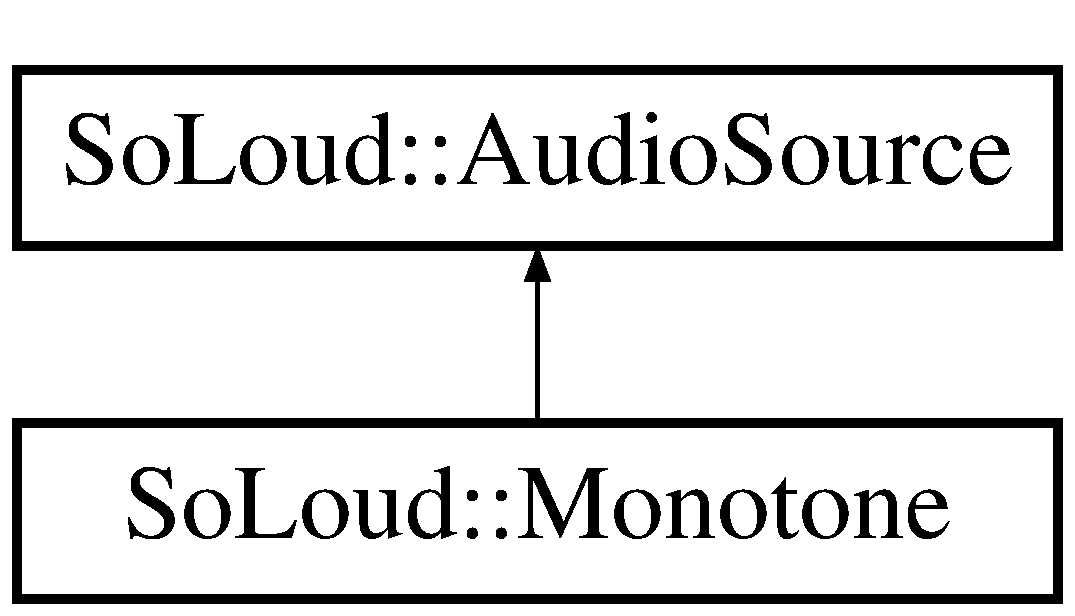
\includegraphics[height=2.000000cm]{class_so_loud_1_1_monotone}
\end{center}
\end{figure}
\subsection*{Public Types}
\begin{DoxyCompactItemize}
\item 
\mbox{\Hypertarget{class_so_loud_1_1_monotone_ae32e37d4bd95aab51d6eb5d293b3c3f3}\label{class_so_loud_1_1_monotone_ae32e37d4bd95aab51d6eb5d293b3c3f3}} 
enum {\bfseries M\+O\+N\+O\+T\+O\+N\+E\+\_\+\+W\+A\+V\+E\+F\+O\+R\+MS} \{ {\bfseries S\+Q\+U\+A\+RE} = 0, 
{\bfseries S\+AW} = 1, 
{\bfseries S\+IN} = 2, 
{\bfseries S\+A\+W\+S\+IN} = 3
 \}
\end{DoxyCompactItemize}
\subsection*{Public Member Functions}
\begin{DoxyCompactItemize}
\item 
\mbox{\Hypertarget{class_so_loud_1_1_monotone_a8bc94c64a4a8e13424f80db6b16a7529}\label{class_so_loud_1_1_monotone_a8bc94c64a4a8e13424f80db6b16a7529}} 
result {\bfseries set\+Params} (int a\+Hardware\+Channels, int a\+Waveform=S\+Q\+U\+A\+RE)
\item 
\mbox{\Hypertarget{class_so_loud_1_1_monotone_a19e67a5264c13d870f4c3530b77bc734}\label{class_so_loud_1_1_monotone_a19e67a5264c13d870f4c3530b77bc734}} 
result {\bfseries load} (const char $\ast$a\+Filename)
\item 
\mbox{\Hypertarget{class_so_loud_1_1_monotone_aae96f6f83f82c2f58b181cac57032403}\label{class_so_loud_1_1_monotone_aae96f6f83f82c2f58b181cac57032403}} 
result {\bfseries load\+Mem} (unsigned char $\ast$a\+Mem, unsigned int a\+Length, bool a\+Copy=false, bool a\+Take\+Ownership=true)
\item 
\mbox{\Hypertarget{class_so_loud_1_1_monotone_ad78047cde881908f8b9c4a198243aa56}\label{class_so_loud_1_1_monotone_ad78047cde881908f8b9c4a198243aa56}} 
result {\bfseries load\+File} (\mbox{\hyperlink{class_so_loud_1_1_file}{File}} $\ast$a\+File)
\item 
\mbox{\Hypertarget{class_so_loud_1_1_monotone_a8d694dbeb32353ceb9f0c40e88985a24}\label{class_so_loud_1_1_monotone_a8d694dbeb32353ceb9f0c40e88985a24}} 
virtual \mbox{\hyperlink{class_so_loud_1_1_audio_source_instance}{Audio\+Source\+Instance}} $\ast$ {\bfseries create\+Instance} ()
\item 
\mbox{\Hypertarget{class_so_loud_1_1_monotone_a2be81352ed0fc38f03530aa241e6a353}\label{class_so_loud_1_1_monotone_a2be81352ed0fc38f03530aa241e6a353}} 
void {\bfseries clear} ()
\end{DoxyCompactItemize}
\subsection*{Public Attributes}
\begin{DoxyCompactItemize}
\item 
\mbox{\Hypertarget{class_so_loud_1_1_monotone_ae9457bde8afdc530f84ac285503b7973}\label{class_so_loud_1_1_monotone_ae9457bde8afdc530f84ac285503b7973}} 
int {\bfseries m\+Notes\+Hz} \mbox{[}800\mbox{]}
\item 
\mbox{\Hypertarget{class_so_loud_1_1_monotone_ab4a409741b4e71777b910e3808ff3d00}\label{class_so_loud_1_1_monotone_ab4a409741b4e71777b910e3808ff3d00}} 
int {\bfseries m\+Vib\+Table} \mbox{[}32\mbox{]}
\item 
\mbox{\Hypertarget{class_so_loud_1_1_monotone_a88755b618ac5fb430bf44ae0da37f9bf}\label{class_so_loud_1_1_monotone_a88755b618ac5fb430bf44ae0da37f9bf}} 
int {\bfseries m\+Hardware\+Channels}
\item 
\mbox{\Hypertarget{class_so_loud_1_1_monotone_ac9a718582a6d8ee99100c30e8299d881}\label{class_so_loud_1_1_monotone_ac9a718582a6d8ee99100c30e8299d881}} 
int {\bfseries m\+Waveform}
\item 
\mbox{\Hypertarget{class_so_loud_1_1_monotone_adceb8944d5607a506b7fd57a9a40c5e7}\label{class_so_loud_1_1_monotone_adceb8944d5607a506b7fd57a9a40c5e7}} 
\mbox{\hyperlink{struct_so_loud_1_1_monotone_song}{Monotone\+Song}} {\bfseries m\+Song}
\end{DoxyCompactItemize}


The documentation for this class was generated from the following file\+:\begin{DoxyCompactItemize}
\item 
deps/\+E\+S\+A\+T/include/\+E\+S\+A\+T\+\_\+extra/soloud/soloud\+\_\+monotone.\+h\end{DoxyCompactItemize}

\hypertarget{struct_so_loud_1_1_monotone_channel}{}\section{So\+Loud\+:\+:Monotone\+Channel Struct Reference}
\label{struct_so_loud_1_1_monotone_channel}\index{So\+Loud\+::\+Monotone\+Channel@{So\+Loud\+::\+Monotone\+Channel}}
\subsection*{Public Attributes}
\begin{DoxyCompactItemize}
\item 
\mbox{\Hypertarget{struct_so_loud_1_1_monotone_channel_a602555f7e6902a92b02cfe919c7429fc}\label{struct_so_loud_1_1_monotone_channel_a602555f7e6902a92b02cfe919c7429fc}} 
int {\bfseries m\+Enabled}
\item 
\mbox{\Hypertarget{struct_so_loud_1_1_monotone_channel_a6be325ad129edc512a8844927d5fdcd9}\label{struct_so_loud_1_1_monotone_channel_a6be325ad129edc512a8844927d5fdcd9}} 
int {\bfseries m\+Active}
\item 
\mbox{\Hypertarget{struct_so_loud_1_1_monotone_channel_acce03d2e79a05ea63be8f30051aebecd}\label{struct_so_loud_1_1_monotone_channel_acce03d2e79a05ea63be8f30051aebecd}} 
int {\bfseries m\+Freq} \mbox{[}3\mbox{]}
\item 
\mbox{\Hypertarget{struct_so_loud_1_1_monotone_channel_a21a22b01af45aeac2897e1f98bbfb6ac}\label{struct_so_loud_1_1_monotone_channel_a21a22b01af45aeac2897e1f98bbfb6ac}} 
int {\bfseries m\+Portamento}
\item 
\mbox{\Hypertarget{struct_so_loud_1_1_monotone_channel_a6663c37a5a349c11af0f1c1b82172ee2}\label{struct_so_loud_1_1_monotone_channel_a6663c37a5a349c11af0f1c1b82172ee2}} 
int {\bfseries m\+Arp\+Counter}
\item 
\mbox{\Hypertarget{struct_so_loud_1_1_monotone_channel_aae4e6376ce89d269496f046851b12bc8}\label{struct_so_loud_1_1_monotone_channel_aae4e6376ce89d269496f046851b12bc8}} 
int {\bfseries m\+Arp}
\item 
\mbox{\Hypertarget{struct_so_loud_1_1_monotone_channel_aecc61199b4a97561b44e1c70c0f45b7a}\label{struct_so_loud_1_1_monotone_channel_aecc61199b4a97561b44e1c70c0f45b7a}} 
int {\bfseries m\+Last\+Note}
\item 
\mbox{\Hypertarget{struct_so_loud_1_1_monotone_channel_a3b224d2b41bfaa83737824c3fb932164}\label{struct_so_loud_1_1_monotone_channel_a3b224d2b41bfaa83737824c3fb932164}} 
int {\bfseries m\+Portamento\+To\+Note}
\item 
\mbox{\Hypertarget{struct_so_loud_1_1_monotone_channel_a3adecd373817c6e7b0ea7094afa2b1ce}\label{struct_so_loud_1_1_monotone_channel_a3adecd373817c6e7b0ea7094afa2b1ce}} 
int {\bfseries m\+Vibrato}
\item 
\mbox{\Hypertarget{struct_so_loud_1_1_monotone_channel_a94f4e3f3b0e29be984095096eb2dc8df}\label{struct_so_loud_1_1_monotone_channel_a94f4e3f3b0e29be984095096eb2dc8df}} 
int {\bfseries m\+Vibrato\+Index}
\item 
\mbox{\Hypertarget{struct_so_loud_1_1_monotone_channel_a66ebdfe63337b787f05901eff3600170}\label{struct_so_loud_1_1_monotone_channel_a66ebdfe63337b787f05901eff3600170}} 
int {\bfseries m\+Vibrato\+Depth}
\item 
\mbox{\Hypertarget{struct_so_loud_1_1_monotone_channel_adf9dce6bb6f6de8c898fe1dc56b7d367}\label{struct_so_loud_1_1_monotone_channel_adf9dce6bb6f6de8c898fe1dc56b7d367}} 
int {\bfseries m\+Vibrato\+Speed}
\end{DoxyCompactItemize}


The documentation for this struct was generated from the following file\+:\begin{DoxyCompactItemize}
\item 
deps/\+E\+S\+A\+T/include/\+E\+S\+A\+T\+\_\+extra/soloud/soloud\+\_\+monotone.\+h\end{DoxyCompactItemize}

\hypertarget{struct_so_loud_1_1_monotone_hardware_channel}{}\section{So\+Loud\+:\+:Monotone\+Hardware\+Channel Struct Reference}
\label{struct_so_loud_1_1_monotone_hardware_channel}\index{So\+Loud\+::\+Monotone\+Hardware\+Channel@{So\+Loud\+::\+Monotone\+Hardware\+Channel}}
\subsection*{Public Attributes}
\begin{DoxyCompactItemize}
\item 
\mbox{\Hypertarget{struct_so_loud_1_1_monotone_hardware_channel_ac9b01626e2c41c0514b5dd5b31e638b3}\label{struct_so_loud_1_1_monotone_hardware_channel_ac9b01626e2c41c0514b5dd5b31e638b3}} 
int {\bfseries m\+Enabled}
\item 
\mbox{\Hypertarget{struct_so_loud_1_1_monotone_hardware_channel_ab174cd3122d83fcd84b4a59f83f1839b}\label{struct_so_loud_1_1_monotone_hardware_channel_ab174cd3122d83fcd84b4a59f83f1839b}} 
float {\bfseries m\+Sample\+Pos}
\item 
\mbox{\Hypertarget{struct_so_loud_1_1_monotone_hardware_channel_a48d914147bfcc40f7060903fe3060540}\label{struct_so_loud_1_1_monotone_hardware_channel_a48d914147bfcc40f7060903fe3060540}} 
float {\bfseries m\+Sample\+Pos\+Inc}
\end{DoxyCompactItemize}


The documentation for this struct was generated from the following file\+:\begin{DoxyCompactItemize}
\item 
deps/\+E\+S\+A\+T/include/\+E\+S\+A\+T\+\_\+extra/soloud/soloud\+\_\+monotone.\+h\end{DoxyCompactItemize}

\hypertarget{class_so_loud_1_1_monotone_instance}{}\section{So\+Loud\+:\+:Monotone\+Instance Class Reference}
\label{class_so_loud_1_1_monotone_instance}\index{So\+Loud\+::\+Monotone\+Instance@{So\+Loud\+::\+Monotone\+Instance}}
Inheritance diagram for So\+Loud\+:\+:Monotone\+Instance\+:\begin{figure}[H]
\begin{center}
\leavevmode
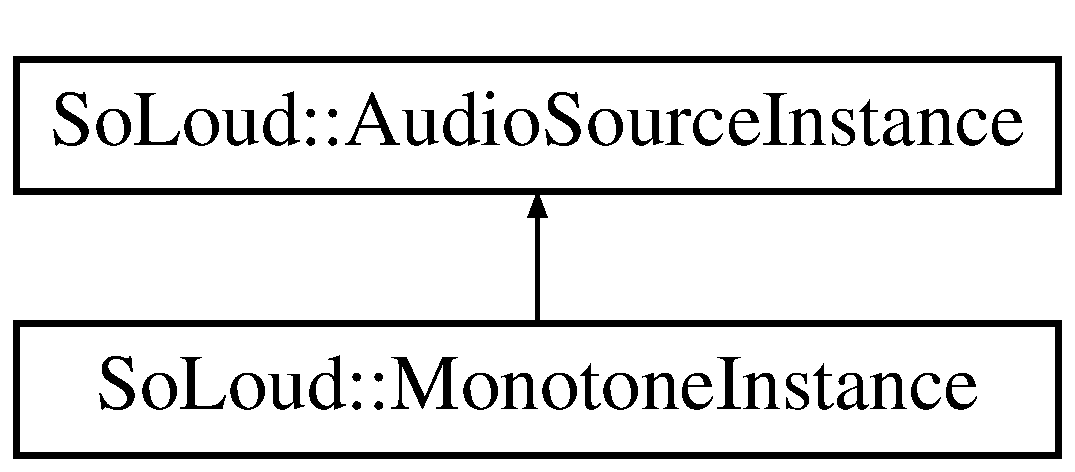
\includegraphics[height=2.000000cm]{class_so_loud_1_1_monotone_instance}
\end{center}
\end{figure}
\subsection*{Public Member Functions}
\begin{DoxyCompactItemize}
\item 
\mbox{\Hypertarget{class_so_loud_1_1_monotone_instance_aca1ab87876b7284b16a9dcdf57d59184}\label{class_so_loud_1_1_monotone_instance_aca1ab87876b7284b16a9dcdf57d59184}} 
{\bfseries Monotone\+Instance} (\mbox{\hyperlink{class_so_loud_1_1_monotone}{Monotone}} $\ast$a\+Parent)
\item 
\mbox{\Hypertarget{class_so_loud_1_1_monotone_instance_a3a52ace28c260e0adb2835095a3ae5f6}\label{class_so_loud_1_1_monotone_instance_a3a52ace28c260e0adb2835095a3ae5f6}} 
virtual void {\bfseries get\+Audio} (float $\ast$a\+Buffer, unsigned int a\+Samples)
\item 
\mbox{\Hypertarget{class_so_loud_1_1_monotone_instance_a0770242189901128b7c4d8eb49d77562}\label{class_so_loud_1_1_monotone_instance_a0770242189901128b7c4d8eb49d77562}} 
virtual bool {\bfseries has\+Ended} ()
\end{DoxyCompactItemize}
\subsection*{Public Attributes}
\begin{DoxyCompactItemize}
\item 
\mbox{\Hypertarget{class_so_loud_1_1_monotone_instance_aee1f7fef30f3e01220ab83e5fa4b180d}\label{class_so_loud_1_1_monotone_instance_aee1f7fef30f3e01220ab83e5fa4b180d}} 
\mbox{\hyperlink{struct_so_loud_1_1_monotone_channel}{Monotone\+Channel}} {\bfseries m\+Channel} \mbox{[}12\mbox{]}
\item 
\mbox{\Hypertarget{class_so_loud_1_1_monotone_instance_adbd0e6190fa7dcc58ff274dd3c9ad140}\label{class_so_loud_1_1_monotone_instance_adbd0e6190fa7dcc58ff274dd3c9ad140}} 
\mbox{\hyperlink{struct_so_loud_1_1_monotone_hardware_channel}{Monotone\+Hardware\+Channel}} {\bfseries m\+Output} \mbox{[}12\mbox{]}
\item 
\mbox{\Hypertarget{class_so_loud_1_1_monotone_instance_a65539fbb341b2155d6f1436d72803a66}\label{class_so_loud_1_1_monotone_instance_a65539fbb341b2155d6f1436d72803a66}} 
int {\bfseries m\+Next\+Channel}
\item 
\mbox{\Hypertarget{class_so_loud_1_1_monotone_instance_ab4153fbdbda4044eef0954f16ad3941f}\label{class_so_loud_1_1_monotone_instance_ab4153fbdbda4044eef0954f16ad3941f}} 
int {\bfseries m\+Tempo}
\item 
\mbox{\Hypertarget{class_so_loud_1_1_monotone_instance_a8ff38937462eef3eb6ac406659d5265e}\label{class_so_loud_1_1_monotone_instance_a8ff38937462eef3eb6ac406659d5265e}} 
int {\bfseries m\+Order}
\item 
\mbox{\Hypertarget{class_so_loud_1_1_monotone_instance_abed652b9aada3dd2dc3bd3d570ab1fba}\label{class_so_loud_1_1_monotone_instance_abed652b9aada3dd2dc3bd3d570ab1fba}} 
int {\bfseries m\+Row}
\item 
\mbox{\Hypertarget{class_so_loud_1_1_monotone_instance_a73cf22d769dc5ff543850b5913775c5b}\label{class_so_loud_1_1_monotone_instance_a73cf22d769dc5ff543850b5913775c5b}} 
int {\bfseries m\+Sample\+Count}
\item 
\mbox{\Hypertarget{class_so_loud_1_1_monotone_instance_ae9b7bff2b72639e579c154be1da031a2}\label{class_so_loud_1_1_monotone_instance_ae9b7bff2b72639e579c154be1da031a2}} 
int {\bfseries m\+Row\+Tick}
\end{DoxyCompactItemize}
\subsection*{Additional Inherited Members}


The documentation for this class was generated from the following file\+:\begin{DoxyCompactItemize}
\item 
deps/\+E\+S\+A\+T/include/\+E\+S\+A\+T\+\_\+extra/soloud/soloud\+\_\+monotone.\+h\end{DoxyCompactItemize}

\hypertarget{struct_so_loud_1_1_monotone_song}{}\section{So\+Loud\+:\+:Monotone\+Song Struct Reference}
\label{struct_so_loud_1_1_monotone_song}\index{So\+Loud\+::\+Monotone\+Song@{So\+Loud\+::\+Monotone\+Song}}
\subsection*{Public Attributes}
\begin{DoxyCompactItemize}
\item 
\mbox{\Hypertarget{struct_so_loud_1_1_monotone_song_ad4dbcdae4046658e37581cd5fde44686}\label{struct_so_loud_1_1_monotone_song_ad4dbcdae4046658e37581cd5fde44686}} 
char $\ast$ {\bfseries m\+Title}
\item 
\mbox{\Hypertarget{struct_so_loud_1_1_monotone_song_a1938dec3e97a6561e7ece26402db4e7f}\label{struct_so_loud_1_1_monotone_song_a1938dec3e97a6561e7ece26402db4e7f}} 
char $\ast$ {\bfseries m\+Comment}
\item 
\mbox{\Hypertarget{struct_so_loud_1_1_monotone_song_a78d84ce7c2f2867d6779ff5a247c7ba1}\label{struct_so_loud_1_1_monotone_song_a78d84ce7c2f2867d6779ff5a247c7ba1}} 
unsigned char {\bfseries m\+Version}
\item 
\mbox{\Hypertarget{struct_so_loud_1_1_monotone_song_a4f17e14176d11f02d30b8fc3294bbe59}\label{struct_so_loud_1_1_monotone_song_a4f17e14176d11f02d30b8fc3294bbe59}} 
unsigned char {\bfseries m\+Total\+Patterns}
\item 
\mbox{\Hypertarget{struct_so_loud_1_1_monotone_song_a9acafb9b59449813cc4b2a5a52cfe077}\label{struct_so_loud_1_1_monotone_song_a9acafb9b59449813cc4b2a5a52cfe077}} 
unsigned char {\bfseries m\+Total\+Tracks}
\item 
\mbox{\Hypertarget{struct_so_loud_1_1_monotone_song_a6a12624368eab485c8f11f3a1afec9e1}\label{struct_so_loud_1_1_monotone_song_a6a12624368eab485c8f11f3a1afec9e1}} 
unsigned char {\bfseries m\+Cell\+Size}
\item 
\mbox{\Hypertarget{struct_so_loud_1_1_monotone_song_a2aee4e18529f975d4643ab1a1e545351}\label{struct_so_loud_1_1_monotone_song_a2aee4e18529f975d4643ab1a1e545351}} 
unsigned char {\bfseries m\+Order} \mbox{[}256\mbox{]}
\item 
\mbox{\Hypertarget{struct_so_loud_1_1_monotone_song_af0268cbc0e458a3b2fae806c65d86649}\label{struct_so_loud_1_1_monotone_song_af0268cbc0e458a3b2fae806c65d86649}} 
unsigned int $\ast$ {\bfseries m\+Pattern\+Data}
\end{DoxyCompactItemize}


The documentation for this struct was generated from the following file\+:\begin{DoxyCompactItemize}
\item 
deps/\+E\+S\+A\+T/include/\+E\+S\+A\+T\+\_\+extra/soloud/soloud\+\_\+monotone.\+h\end{DoxyCompactItemize}

\hypertarget{struct_e_s_a_t_1_1_network_address}{}\section{E\+S\+AT\+:\+:Network\+Address Struct Reference}
\label{struct_e_s_a_t_1_1_network_address}\index{E\+S\+A\+T\+::\+Network\+Address@{E\+S\+A\+T\+::\+Network\+Address}}
\subsection*{Public Attributes}
\begin{DoxyCompactItemize}
\item 
\mbox{\Hypertarget{struct_e_s_a_t_1_1_network_address_a2beb3caf9819e39fbe2c1cdad89d27ca}\label{struct_e_s_a_t_1_1_network_address_a2beb3caf9819e39fbe2c1cdad89d27ca}} 
const char $\ast$ {\bfseries address}
\item 
\mbox{\Hypertarget{struct_e_s_a_t_1_1_network_address_a31d1014be107d088f28b503c32b68612}\label{struct_e_s_a_t_1_1_network_address_a31d1014be107d088f28b503c32b68612}} 
unsigned int {\bfseries port}
\end{DoxyCompactItemize}


The documentation for this struct was generated from the following file\+:\begin{DoxyCompactItemize}
\item 
deps/\+E\+S\+A\+T/include/\+E\+S\+A\+T/network.\+h\end{DoxyCompactItemize}

\hypertarget{struct_im_gui_storage_1_1_pair}{}\section{Im\+Gui\+Storage\+:\+:Pair Struct Reference}
\label{struct_im_gui_storage_1_1_pair}\index{Im\+Gui\+Storage\+::\+Pair@{Im\+Gui\+Storage\+::\+Pair}}
\subsection*{Public Member Functions}
\begin{DoxyCompactItemize}
\item 
\mbox{\Hypertarget{struct_im_gui_storage_1_1_pair_a37542a22048f0af35e5a6beda6900a0e}\label{struct_im_gui_storage_1_1_pair_a37542a22048f0af35e5a6beda6900a0e}} 
{\bfseries Pair} (Im\+Gui\+ID \+\_\+key, int \+\_\+val\+\_\+i)
\item 
\mbox{\Hypertarget{struct_im_gui_storage_1_1_pair_a6f63f598513f2a7a57f2e9ea3b0137b9}\label{struct_im_gui_storage_1_1_pair_a6f63f598513f2a7a57f2e9ea3b0137b9}} 
{\bfseries Pair} (Im\+Gui\+ID \+\_\+key, float \+\_\+val\+\_\+f)
\item 
\mbox{\Hypertarget{struct_im_gui_storage_1_1_pair_a4d07d60f83b4e24ee8be9ccceaab76bd}\label{struct_im_gui_storage_1_1_pair_a4d07d60f83b4e24ee8be9ccceaab76bd}} 
{\bfseries Pair} (Im\+Gui\+ID \+\_\+key, void $\ast$\+\_\+val\+\_\+p)
\end{DoxyCompactItemize}
\subsection*{Public Attributes}
\begin{DoxyCompactItemize}
\item 
\mbox{\Hypertarget{struct_im_gui_storage_1_1_pair_a5b37b692d2eacc7f4f5b6f233359e6ce}\label{struct_im_gui_storage_1_1_pair_a5b37b692d2eacc7f4f5b6f233359e6ce}} 
Im\+Gui\+ID {\bfseries key}
\item 
\mbox{\Hypertarget{struct_im_gui_storage_1_1_pair_acb7e084ac6a610d3b721737494cf776d}\label{struct_im_gui_storage_1_1_pair_acb7e084ac6a610d3b721737494cf776d}} 
\begin{tabbing}
xx\=xx\=xx\=xx\=xx\=xx\=xx\=xx\=xx\=\kill
union \{\\
\>int {\bfseries val\_i}\\
\>float {\bfseries val\_f}\\
\>void $\ast$ {\bfseries val\_p}\\
\}; \\

\end{tabbing}\end{DoxyCompactItemize}


The documentation for this struct was generated from the following file\+:\begin{DoxyCompactItemize}
\item 
deps/\+E\+S\+A\+T/include/\+E\+S\+A\+T\+\_\+extra/imgui.\+h\end{DoxyCompactItemize}

\hypertarget{class_path}{}\section{Path Class Reference}
\label{class_path}\index{Path@{Path}}


\mbox{\hyperlink{class_path}{Path}} class.  




{\ttfamily \#include $<$path.\+h$>$}

\subsection*{Public Member Functions}
\begin{DoxyCompactItemize}
\item 
\mbox{\hyperlink{class_path_af26cfab021ddf49af73da3b2beca85ac}{Path}} ()
\begin{DoxyCompactList}\small\item\em \mbox{\hyperlink{class_path}{Path}} constructor. \end{DoxyCompactList}\item 
\mbox{\hyperlink{class_path_a141da9ff89c85e0ba410b5a73864c267}{$\sim$\+Path}} ()
\begin{DoxyCompactList}\small\item\em Destroys the \mbox{\hyperlink{class_path}{Path}}. \end{DoxyCompactList}\item 
s16 \mbox{\hyperlink{class_path_a04a6c286852f3b7f53a187e25b38f3ec}{create}} (u16 points=50)
\begin{DoxyCompactList}\small\item\em creates a \mbox{\hyperlink{class_path}{Path}} \end{DoxyCompactList}\item 
s16 \mbox{\hyperlink{class_path_a8337c002364b617cec92d1d141592847}{set\+To\+Ready}} ()
\begin{DoxyCompactList}\small\item\em sets the path to a ready state \end{DoxyCompactList}\item 
s16 \mbox{\hyperlink{class_path_a7569f8a9cfbba8324ea9029db7afe7fc}{set\+\_\+direction}} (Direction direction)
\begin{DoxyCompactList}\small\item\em sets the direction of the path \end{DoxyCompactList}\item 
s16 \mbox{\hyperlink{class_path_a94fc077d91eb4440744713303309fe4d}{set\+\_\+action}} (Action action)
\begin{DoxyCompactList}\small\item\em sets the action of the path \end{DoxyCompactList}\item 
s16 \mbox{\hyperlink{class_path_a9932d1c9742ab5c9bf1d2fea0536c0ad}{set\+\_\+action}} (Action action, s16 loops)
\begin{DoxyCompactList}\small\item\em sets the action of the path \end{DoxyCompactList}\item 
s16 \mbox{\hyperlink{class_path_aec0977970beeaa279c2c3f152aee0f88}{add\+Point}} (float x, float y)
\begin{DoxyCompactList}\small\item\em adds a new point to the path \end{DoxyCompactList}\item 
s16 \mbox{\hyperlink{class_path_a114453983549b6be3d27788272d26b2a}{add\+Point}} (\mbox{\hyperlink{class_float2}{Float2}} $\ast$new\+\_\+point)
\begin{DoxyCompactList}\small\item\em adds a new point to the path \end{DoxyCompactList}\item 
bool \mbox{\hyperlink{class_path_aeb7e40ba58a329fb01053f72ef0a6d56}{is\+Last}} ()
\begin{DoxyCompactList}\small\item\em informs if the current point of the path is the las one \end{DoxyCompactList}\item 
bool \mbox{\hyperlink{class_path_a738ebaf508fc4a35dd5a5f5f8c84e39f}{is\+Ready}} ()
\begin{DoxyCompactList}\small\item\em informs if the path is ready to be used \end{DoxyCompactList}\item 
\mbox{\hyperlink{class_float2}{Float2}} const  $\ast$ \mbox{\hyperlink{class_path_a17f70e35a36c29650f571c59a237b0e5}{next\+Point}} ()
\begin{DoxyCompactList}\small\item\em Gets the next point of the path. \end{DoxyCompactList}\item 
\mbox{\hyperlink{class_float2}{Float2}} const  $\ast$ \mbox{\hyperlink{class_path_af5da5742823a638b5bf9100b3f0b37ea}{prev\+Point}} ()
\begin{DoxyCompactList}\small\item\em Gets the prev point of the path. \end{DoxyCompactList}\item 
\mbox{\hyperlink{class_float2}{Float2}} const  $\ast$ \mbox{\hyperlink{class_path_a2ef24ce0bf3b3468ecbb4a6e0efdebfd}{last\+Point}} ()
\begin{DoxyCompactList}\small\item\em Gets the last point of the path. \end{DoxyCompactList}\end{DoxyCompactItemize}
\subsection*{Public Attributes}
\begin{DoxyCompactItemize}
\item 
\mbox{\Hypertarget{class_path_a7cb1f774525b1c0a68dac6e01dc10121}\label{class_path_a7cb1f774525b1c0a68dac6e01dc10121}} 
u16 {\bfseries total\+\_\+points\+\_\+}
\end{DoxyCompactItemize}


\subsection{Detailed Description}
\mbox{\hyperlink{class_path}{Path}} class. 

Class in charge of storing sets of points, it also stores rules to indicate how we want to traverse those points. 

\subsection{Constructor \& Destructor Documentation}
\mbox{\Hypertarget{class_path_af26cfab021ddf49af73da3b2beca85ac}\label{class_path_af26cfab021ddf49af73da3b2beca85ac}} 
\index{Path@{Path}!Path@{Path}}
\index{Path@{Path}!Path@{Path}}
\subsubsection{\texorpdfstring{Path()}{Path()}}
{\footnotesize\ttfamily Path\+::\+Path (\begin{DoxyParamCaption}{ }\end{DoxyParamCaption})}



\mbox{\hyperlink{class_path}{Path}} constructor. 

Constructor of path. Sets the state to a default one, note that the path is not ready after the construcotr.

\begin{DoxyReturn}{Returns}
$\ast$\+Agent 
\end{DoxyReturn}
\mbox{\Hypertarget{class_path_a141da9ff89c85e0ba410b5a73864c267}\label{class_path_a141da9ff89c85e0ba410b5a73864c267}} 
\index{Path@{Path}!````~Path@{$\sim$\+Path}}
\index{````~Path@{$\sim$\+Path}!Path@{Path}}
\subsubsection{\texorpdfstring{$\sim$\+Path()}{~Path()}}
{\footnotesize\ttfamily Path\+::$\sim$\+Path (\begin{DoxyParamCaption}{ }\end{DoxyParamCaption})}



Destroys the \mbox{\hyperlink{class_path}{Path}}. 

Destructor of the path

\begin{DoxyReturn}{Returns}
void 
\end{DoxyReturn}


\subsection{Member Function Documentation}
\mbox{\Hypertarget{class_path_aec0977970beeaa279c2c3f152aee0f88}\label{class_path_aec0977970beeaa279c2c3f152aee0f88}} 
\index{Path@{Path}!add\+Point@{add\+Point}}
\index{add\+Point@{add\+Point}!Path@{Path}}
\subsubsection{\texorpdfstring{add\+Point()}{addPoint()}\hspace{0.1cm}{\footnotesize\ttfamily [1/2]}}
{\footnotesize\ttfamily s16 Path\+::add\+Point (\begin{DoxyParamCaption}\item[{float}]{x,  }\item[{float}]{y }\end{DoxyParamCaption})}



adds a new point to the path 

Adds a new point to the path. Note that if the path is already full or has not been created this function will return an error


\begin{DoxyParams}{Parameters}
{\em x} & x coordinate of the point \\
\hline
{\em y} & y coordinate of the point \\
\hline
\end{DoxyParams}
\begin{DoxyReturn}{Returns}
s16 result of the operation 
\end{DoxyReturn}
\mbox{\Hypertarget{class_path_a114453983549b6be3d27788272d26b2a}\label{class_path_a114453983549b6be3d27788272d26b2a}} 
\index{Path@{Path}!add\+Point@{add\+Point}}
\index{add\+Point@{add\+Point}!Path@{Path}}
\subsubsection{\texorpdfstring{add\+Point()}{addPoint()}\hspace{0.1cm}{\footnotesize\ttfamily [2/2]}}
{\footnotesize\ttfamily s16 Path\+::add\+Point (\begin{DoxyParamCaption}\item[{\mbox{\hyperlink{class_float2}{Float2}} $\ast$}]{new\+\_\+point }\end{DoxyParamCaption})}



adds a new point to the path 

Adds a new point to the path. Note that if the path is already full or has not been created this function will return an error


\begin{DoxyParams}{Parameters}
{\em new\+\_\+point} & point to be added \\
\hline
\end{DoxyParams}
\begin{DoxyReturn}{Returns}
s16 result of the operation 
\end{DoxyReturn}
\mbox{\Hypertarget{class_path_a04a6c286852f3b7f53a187e25b38f3ec}\label{class_path_a04a6c286852f3b7f53a187e25b38f3ec}} 
\index{Path@{Path}!create@{create}}
\index{create@{create}!Path@{Path}}
\subsubsection{\texorpdfstring{create()}{create()}}
{\footnotesize\ttfamily s16 Path\+::create (\begin{DoxyParamCaption}\item[{u16}]{points = {\ttfamily 50} }\end{DoxyParamCaption})}



creates a \mbox{\hyperlink{class_path}{Path}} 

Allocates the memory that the path will have. Note that passing 0 points ore more than the k\+Max\+Points will result in a k\+Error\+Code\+\_\+\+Incorrect\+Points\+Number. Otherwise if all went correct a k\+Error\+Code\+\_\+\+Ok will be returned. This function clears and initializes any data that was stored in the path previously if any.


\begin{DoxyParams}{Parameters}
{\em points} & number of points that will have the path \\
\hline
\end{DoxyParams}
\begin{DoxyReturn}{Returns}
s16 result of the operation 
\end{DoxyReturn}
\mbox{\Hypertarget{class_path_aeb7e40ba58a329fb01053f72ef0a6d56}\label{class_path_aeb7e40ba58a329fb01053f72ef0a6d56}} 
\index{Path@{Path}!is\+Last@{is\+Last}}
\index{is\+Last@{is\+Last}!Path@{Path}}
\subsubsection{\texorpdfstring{is\+Last()}{isLast()}}
{\footnotesize\ttfamily bool Path\+::is\+Last (\begin{DoxyParamCaption}{ }\end{DoxyParamCaption})}



informs if the current point of the path is the las one 

Informs if the current point of the path is the las one. True if it is the last one false otherwise

\begin{DoxyReturn}{Returns}
bool result of the operation 
\end{DoxyReturn}
\mbox{\Hypertarget{class_path_a738ebaf508fc4a35dd5a5f5f8c84e39f}\label{class_path_a738ebaf508fc4a35dd5a5f5f8c84e39f}} 
\index{Path@{Path}!is\+Ready@{is\+Ready}}
\index{is\+Ready@{is\+Ready}!Path@{Path}}
\subsubsection{\texorpdfstring{is\+Ready()}{isReady()}}
{\footnotesize\ttfamily bool Path\+::is\+Ready (\begin{DoxyParamCaption}{ }\end{DoxyParamCaption})}



informs if the path is ready to be used 

Informs if the path is ready to be used. True if it is the last one false otherwise

\begin{DoxyReturn}{Returns}
bool result of the operation 
\end{DoxyReturn}
\mbox{\Hypertarget{class_path_a2ef24ce0bf3b3468ecbb4a6e0efdebfd}\label{class_path_a2ef24ce0bf3b3468ecbb4a6e0efdebfd}} 
\index{Path@{Path}!last\+Point@{last\+Point}}
\index{last\+Point@{last\+Point}!Path@{Path}}
\subsubsection{\texorpdfstring{last\+Point()}{lastPoint()}}
{\footnotesize\ttfamily \mbox{\hyperlink{class_float2}{Float2}} const  $\ast$ Path\+::last\+Point (\begin{DoxyParamCaption}{ }\end{DoxyParamCaption})}



Gets the last point of the path. 

Gets the last point of the path. In case the path is not ready it will return nullptr.

\begin{DoxyReturn}{Returns}
\mbox{\hyperlink{class_float2}{Float2}} last point of the path 
\end{DoxyReturn}
\mbox{\Hypertarget{class_path_a17f70e35a36c29650f571c59a237b0e5}\label{class_path_a17f70e35a36c29650f571c59a237b0e5}} 
\index{Path@{Path}!next\+Point@{next\+Point}}
\index{next\+Point@{next\+Point}!Path@{Path}}
\subsubsection{\texorpdfstring{next\+Point()}{nextPoint()}}
{\footnotesize\ttfamily \mbox{\hyperlink{class_float2}{Float2}} const  $\ast$ Path\+::next\+Point (\begin{DoxyParamCaption}{ }\end{DoxyParamCaption})}



Gets the next point of the path. 

Gets the next point of the path. In case the path is not ready or there is no next point it will return nullptr.

\begin{DoxyReturn}{Returns}
\mbox{\hyperlink{class_float2}{Float2}} next point of the path 
\end{DoxyReturn}
\mbox{\Hypertarget{class_path_af5da5742823a638b5bf9100b3f0b37ea}\label{class_path_af5da5742823a638b5bf9100b3f0b37ea}} 
\index{Path@{Path}!prev\+Point@{prev\+Point}}
\index{prev\+Point@{prev\+Point}!Path@{Path}}
\subsubsection{\texorpdfstring{prev\+Point()}{prevPoint()}}
{\footnotesize\ttfamily \mbox{\hyperlink{class_float2}{Float2}} const  $\ast$ Path\+::prev\+Point (\begin{DoxyParamCaption}{ }\end{DoxyParamCaption})}



Gets the prev point of the path. 

Gets the prev point of the path.\+In case the path is not ready or there is no prev point it will return nullptr.

\begin{DoxyReturn}{Returns}
\mbox{\hyperlink{class_float2}{Float2}} prev point of the path 
\end{DoxyReturn}
\mbox{\Hypertarget{class_path_a94fc077d91eb4440744713303309fe4d}\label{class_path_a94fc077d91eb4440744713303309fe4d}} 
\index{Path@{Path}!set\+\_\+action@{set\+\_\+action}}
\index{set\+\_\+action@{set\+\_\+action}!Path@{Path}}
\subsubsection{\texorpdfstring{set\+\_\+action()}{set\_action()}\hspace{0.1cm}{\footnotesize\ttfamily [1/2]}}
{\footnotesize\ttfamily s16 Path\+::set\+\_\+action (\begin{DoxyParamCaption}\item[{Action}]{action }\end{DoxyParamCaption})}



sets the action of the path 

Sets the action of the path\+: k\+Action\+None -\/$>$ setting with no loops k\+Action\+Straight -\/$>$ setting with no loops k\+Action\+Loop\+Infinite -\/$>$ Once the path is finished it will start from the start again k\+Action\+Loop\+N\+Times -\/$>$ Will result in an error k\+Error\+Code\+\_\+\+Bad\+Loops\+Setting, please use the set action function that accepts loops


\begin{DoxyParams}{Parameters}
{\em action} & that will use the path \\
\hline
\end{DoxyParams}
\begin{DoxyReturn}{Returns}
s16 result of the operation 
\end{DoxyReturn}
\mbox{\Hypertarget{class_path_a9932d1c9742ab5c9bf1d2fea0536c0ad}\label{class_path_a9932d1c9742ab5c9bf1d2fea0536c0ad}} 
\index{Path@{Path}!set\+\_\+action@{set\+\_\+action}}
\index{set\+\_\+action@{set\+\_\+action}!Path@{Path}}
\subsubsection{\texorpdfstring{set\+\_\+action()}{set\_action()}\hspace{0.1cm}{\footnotesize\ttfamily [2/2]}}
{\footnotesize\ttfamily s16 Path\+::set\+\_\+action (\begin{DoxyParamCaption}\item[{Action}]{action,  }\item[{s16}]{loops }\end{DoxyParamCaption})}



sets the action of the path 

Sets the action of the path. Use this function to set a k\+Action\+Loop\+N\+Times. Otherwise the function will return an error. k\+Action\+Loop\+N\+Times -\/$>$ Once the path is finished it will start from the start again N times


\begin{DoxyParams}{Parameters}
{\em action} & that will use the path \\
\hline
{\em loops} & the number of times the path will be repeated \\
\hline
\end{DoxyParams}
\begin{DoxyReturn}{Returns}
s16 result of the operation 
\end{DoxyReturn}
\mbox{\Hypertarget{class_path_a7569f8a9cfbba8324ea9029db7afe7fc}\label{class_path_a7569f8a9cfbba8324ea9029db7afe7fc}} 
\index{Path@{Path}!set\+\_\+direction@{set\+\_\+direction}}
\index{set\+\_\+direction@{set\+\_\+direction}!Path@{Path}}
\subsubsection{\texorpdfstring{set\+\_\+direction()}{set\_direction()}}
{\footnotesize\ttfamily s16 Path\+::set\+\_\+direction (\begin{DoxyParamCaption}\item[{Direction}]{direction }\end{DoxyParamCaption})}



sets the direction of the path 

Sets the direction of the path\+: k\+Dir\+None -\/$>$ Invalid direction k\+Dir\+Forward -\/$>$ The path will go from the first point to the last one


\begin{DoxyParams}{Parameters}
{\em direction} & that will use the path \\
\hline
\end{DoxyParams}
\begin{DoxyReturn}{Returns}
s16 result of the operation 
\end{DoxyReturn}
\mbox{\Hypertarget{class_path_a8337c002364b617cec92d1d141592847}\label{class_path_a8337c002364b617cec92d1d141592847}} 
\index{Path@{Path}!set\+To\+Ready@{set\+To\+Ready}}
\index{set\+To\+Ready@{set\+To\+Ready}!Path@{Path}}
\subsubsection{\texorpdfstring{set\+To\+Ready()}{setToReady()}}
{\footnotesize\ttfamily s16 Path\+::set\+To\+Ready (\begin{DoxyParamCaption}{ }\end{DoxyParamCaption})}



sets the path to a ready state 

Checks that everything was correctly initialized, if that\textquotesingle{}s the case sets the path to ready and from that point the path can be used. Please check the error code to know more info about the reason why the operation fails. k\+Error\+Code\+\_\+\+Empty\+Path -\/$>$ The path is empty. k\+Error\+Code\+\_\+\+Path\+Not\+Created -\/$>$ The path has not been created. Make sure you called \mbox{\hyperlink{class_path_a04a6c286852f3b7f53a187e25b38f3ec}{create()}} before set\+To\+Ready k\+Error\+Code\+\_\+\+Bad\+Loops\+Setting -\/$>$ The loop setting has not been correctly configured. k\+Error\+Code\+\_\+\+Bad\+Direction\+Setting -\/$>$ The direction setting has not been correctly configured.

\begin{DoxyReturn}{Returns}
s16 result of the operation 
\end{DoxyReturn}


The documentation for this class was generated from the following files\+:\begin{DoxyCompactItemize}
\item 
include/\mbox{\hyperlink{path_8h}{path.\+h}}\item 
src/path.\+cc\end{DoxyCompactItemize}

\hypertarget{class_path_finder}{}\section{Path\+Finder Class Reference}
\label{class_path_finder}\index{Path\+Finder@{Path\+Finder}}


\mbox{\hyperlink{class_path_finder}{Path\+Finder}} agentt.  




{\ttfamily \#include $<$path\+\_\+finder.\+h$>$}

\subsection*{Public Member Functions}
\begin{DoxyCompactItemize}
\item 
\mbox{\hyperlink{class_path_finder_a0761f248c1ebaacf3e47a4021ca25256}{Path\+Finder}} ()
\begin{DoxyCompactList}\small\item\em Pathfinder \mbox{\hyperlink{class_agent}{Agent}} constructor. \end{DoxyCompactList}\item 
\mbox{\hyperlink{class_path_finder_acc04bc8bcddfda54da6a2905b256cf90}{$\sim$\+Path\+Finder}} ()
\begin{DoxyCompactList}\small\item\em Destroys the \mbox{\hyperlink{class_path_finder}{Path\+Finder}}. \end{DoxyCompactList}\item 
s16 \mbox{\hyperlink{class_path_finder_ae1c25582d9f8c1ee73d5adc780a14e9c}{generate\+Path}} (\mbox{\hyperlink{class_path}{Path}} $\ast$path, \mbox{\hyperlink{class_float2}{Float2}} origin, \mbox{\hyperlink{class_float2}{Float2}} dst, u32 timeout)
\begin{DoxyCompactList}\small\item\em generates a path from origin to dst within a time \end{DoxyCompactList}\item 
s16 \mbox{\hyperlink{class_path_finder_a05e232f67bd66be0ef2b56c455dd1425}{generate\+Path}} (\mbox{\hyperlink{class_path}{Path}} $\ast$path, \mbox{\hyperlink{class_float2}{Float2}} origin, \mbox{\hyperlink{class_float2}{Float2}} dst)
\begin{DoxyCompactList}\small\item\em generates a path from origin to dst \end{DoxyCompactList}\item 
void \mbox{\hyperlink{class_path_finder_a45e15457e0f7177c973213cc46722275}{update}} (const u32 dt)
\begin{DoxyCompactList}\small\item\em Updates the agent. \end{DoxyCompactList}\item 
void \mbox{\hyperlink{class_path_finder_a611da8a914a8eebf13af130a6436902a}{update\+Mind}} (const u32 dt)
\begin{DoxyCompactList}\small\item\em Updates the mind of the agent. \end{DoxyCompactList}\item 
void \mbox{\hyperlink{class_path_finder_a4dc676609f38e4809f4b614b2a414235}{update\+Body}} (const u32 dt)
\begin{DoxyCompactList}\small\item\em Updates the body of the agent. \end{DoxyCompactList}\item 
void \mbox{\hyperlink{class_path_finder_afe58142744ff067c1f510efd3478e634}{send\+Message}} (const \mbox{\hyperlink{class_agent_message}{Agent\+Message}} msg, const u32 id)
\begin{DoxyCompactList}\small\item\em function to receive a message from another agent \end{DoxyCompactList}\end{DoxyCompactItemize}


\subsection{Detailed Description}
\mbox{\hyperlink{class_path_finder}{Path\+Finder}} agentt. 

This class is an agent that can be asked for paths. He utilizes the A$\ast$ algorithm to calculate them 

\subsection{Constructor \& Destructor Documentation}
\mbox{\Hypertarget{class_path_finder_a0761f248c1ebaacf3e47a4021ca25256}\label{class_path_finder_a0761f248c1ebaacf3e47a4021ca25256}} 
\index{Path\+Finder@{Path\+Finder}!Path\+Finder@{Path\+Finder}}
\index{Path\+Finder@{Path\+Finder}!Path\+Finder@{Path\+Finder}}
\subsubsection{\texorpdfstring{Path\+Finder()}{PathFinder()}}
{\footnotesize\ttfamily Path\+Finder\+::\+Path\+Finder (\begin{DoxyParamCaption}{ }\end{DoxyParamCaption})}



Pathfinder \mbox{\hyperlink{class_agent}{Agent}} constructor. 

Default pathfinder agent constructor

\begin{DoxyReturn}{Returns}
$\ast$\+Path\+Finder 
\end{DoxyReturn}
\mbox{\Hypertarget{class_path_finder_acc04bc8bcddfda54da6a2905b256cf90}\label{class_path_finder_acc04bc8bcddfda54da6a2905b256cf90}} 
\index{Path\+Finder@{Path\+Finder}!````~Path\+Finder@{$\sim$\+Path\+Finder}}
\index{````~Path\+Finder@{$\sim$\+Path\+Finder}!Path\+Finder@{Path\+Finder}}
\subsubsection{\texorpdfstring{$\sim$\+Path\+Finder()}{~PathFinder()}}
{\footnotesize\ttfamily Path\+Finder\+::$\sim$\+Path\+Finder (\begin{DoxyParamCaption}{ }\end{DoxyParamCaption})}



Destroys the \mbox{\hyperlink{class_path_finder}{Path\+Finder}}. 

Destructor of the pathfinder agent entity

\begin{DoxyReturn}{Returns}
void 
\end{DoxyReturn}


\subsection{Member Function Documentation}
\mbox{\Hypertarget{class_path_finder_ae1c25582d9f8c1ee73d5adc780a14e9c}\label{class_path_finder_ae1c25582d9f8c1ee73d5adc780a14e9c}} 
\index{Path\+Finder@{Path\+Finder}!generate\+Path@{generate\+Path}}
\index{generate\+Path@{generate\+Path}!Path\+Finder@{Path\+Finder}}
\subsubsection{\texorpdfstring{generate\+Path()}{generatePath()}\hspace{0.1cm}{\footnotesize\ttfamily [1/2]}}
{\footnotesize\ttfamily s16 Path\+Finder\+::generate\+Path (\begin{DoxyParamCaption}\item[{\mbox{\hyperlink{class_path}{Path}} $\ast$}]{path,  }\item[{\mbox{\hyperlink{class_float2}{Float2}}}]{origin,  }\item[{\mbox{\hyperlink{class_float2}{Float2}}}]{dst,  }\item[{u32}]{timeout }\end{DoxyParamCaption})}



generates a path from origin to dst within a time 

Starts the generation of a path.

The possible values it can return are\+: k\+Error\+Code\+\_\+\+Invalid\+Origin if the origin is not a valid position k\+Error\+Code\+\_\+\+Invalid\+Destination if dst is not a valid position k\+Error\+Code\+\_\+\+Memory in case the function was unable to allocate new memory k\+Error\+Code\+\_\+\+Path\+Not\+Created k\+Error\+Code\+\_\+\+Path\+Not\+Found if there\textquotesingle{}s not a path that connects origin and dst k\+Error\+Code\+\_\+\+Timeout the A$\ast$ did not finish to calculate the path. The next time generate path is called it will continue from the last point. k\+Error\+Code\+\_\+\+Ok the path was correctly calculated


\begin{DoxyParams}{Parameters}
{\em path} & \mbox{\hyperlink{class_path}{Path}} in which the result will be stored \\
\hline
{\em origin} & origin point from which the path will be calculated \\
\hline
{\em dst} & \mbox{\hyperlink{class_path}{Path}} in which the result will be stored \\
\hline
{\em timeout} & Total time to calculate the path \\
\hline
\end{DoxyParams}
\begin{DoxyReturn}{Returns}
s16 
\end{DoxyReturn}
\mbox{\Hypertarget{class_path_finder_a05e232f67bd66be0ef2b56c455dd1425}\label{class_path_finder_a05e232f67bd66be0ef2b56c455dd1425}} 
\index{Path\+Finder@{Path\+Finder}!generate\+Path@{generate\+Path}}
\index{generate\+Path@{generate\+Path}!Path\+Finder@{Path\+Finder}}
\subsubsection{\texorpdfstring{generate\+Path()}{generatePath()}\hspace{0.1cm}{\footnotesize\ttfamily [2/2]}}
{\footnotesize\ttfamily s16 Path\+Finder\+::generate\+Path (\begin{DoxyParamCaption}\item[{\mbox{\hyperlink{class_path}{Path}} $\ast$}]{path,  }\item[{\mbox{\hyperlink{class_float2}{Float2}}}]{origin,  }\item[{\mbox{\hyperlink{class_float2}{Float2}}}]{dst }\end{DoxyParamCaption})}



generates a path from origin to dst 

Starts the generation of a path.

The possible values it can return are\+: k\+Error\+Code\+\_\+\+Invalid\+Origin if the origin is not a valid position k\+Error\+Code\+\_\+\+Invalid\+Destination if dst is not a valid position k\+Error\+Code\+\_\+\+Memory in case the function was unable to allocate new memory k\+Error\+Code\+\_\+\+Path\+Not\+Created k\+Error\+Code\+\_\+\+Path\+Not\+Found if there\textquotesingle{}s not a path that connects origin and dst k\+Error\+Code\+\_\+\+Ok the path was correctly calculated


\begin{DoxyParams}{Parameters}
{\em path} & \mbox{\hyperlink{class_path}{Path}} in which the result will be stored \\
\hline
{\em origin} & origin point from which the path will be calculated \\
\hline
{\em dst} & \mbox{\hyperlink{class_path}{Path}} in which the result will be stored \\
\hline
\end{DoxyParams}
\begin{DoxyReturn}{Returns}
s16 
\end{DoxyReturn}
\mbox{\Hypertarget{class_path_finder_afe58142744ff067c1f510efd3478e634}\label{class_path_finder_afe58142744ff067c1f510efd3478e634}} 
\index{Path\+Finder@{Path\+Finder}!send\+Message@{send\+Message}}
\index{send\+Message@{send\+Message}!Path\+Finder@{Path\+Finder}}
\subsubsection{\texorpdfstring{send\+Message()}{sendMessage()}}
{\footnotesize\ttfamily void Path\+Finder\+::send\+Message (\begin{DoxyParamCaption}\item[{const \mbox{\hyperlink{class_agent_message}{Agent\+Message}}}]{msg,  }\item[{const u32}]{id }\end{DoxyParamCaption})}



function to receive a message from another agent 

Function to send a message to the agent. This message will be treated at the update\+Mind function.


\begin{DoxyParams}{Parameters}
{\em msg} & content of the message sent \\
\hline
{\em id} & of the one who sent the message\\
\hline
\end{DoxyParams}
\begin{DoxyReturn}{Returns}
void 
\end{DoxyReturn}
\mbox{\Hypertarget{class_path_finder_a45e15457e0f7177c973213cc46722275}\label{class_path_finder_a45e15457e0f7177c973213cc46722275}} 
\index{Path\+Finder@{Path\+Finder}!update@{update}}
\index{update@{update}!Path\+Finder@{Path\+Finder}}
\subsubsection{\texorpdfstring{update()}{update()}}
{\footnotesize\ttfamily void Path\+Finder\+::update (\begin{DoxyParamCaption}\item[{const u32}]{dt }\end{DoxyParamCaption})}



Updates the agent. 

Updates the body and mind of the agent based on a delta time


\begin{DoxyParams}{Parameters}
{\em dt} & time that has passed in the game world \\
\hline
\end{DoxyParams}
\begin{DoxyReturn}{Returns}
void 
\end{DoxyReturn}
\mbox{\Hypertarget{class_path_finder_a4dc676609f38e4809f4b614b2a414235}\label{class_path_finder_a4dc676609f38e4809f4b614b2a414235}} 
\index{Path\+Finder@{Path\+Finder}!update\+Body@{update\+Body}}
\index{update\+Body@{update\+Body}!Path\+Finder@{Path\+Finder}}
\subsubsection{\texorpdfstring{update\+Body()}{updateBody()}}
{\footnotesize\ttfamily void Path\+Finder\+::update\+Body (\begin{DoxyParamCaption}\item[{const u32}]{dt }\end{DoxyParamCaption})}



Updates the body of the agent. 

Updates the physic representation of the agent. Deals with the movement and updates the sensors. This agent does not have representation so this function is empty.


\begin{DoxyParams}{Parameters}
{\em dt} & time that has passed in the game world \\
\hline
\end{DoxyParams}
\begin{DoxyReturn}{Returns}
void 
\end{DoxyReturn}
\mbox{\Hypertarget{class_path_finder_a611da8a914a8eebf13af130a6436902a}\label{class_path_finder_a611da8a914a8eebf13af130a6436902a}} 
\index{Path\+Finder@{Path\+Finder}!update\+Mind@{update\+Mind}}
\index{update\+Mind@{update\+Mind}!Path\+Finder@{Path\+Finder}}
\subsubsection{\texorpdfstring{update\+Mind()}{updateMind()}}
{\footnotesize\ttfamily void Path\+Finder\+::update\+Mind (\begin{DoxyParamCaption}\item[{const u32}]{dt }\end{DoxyParamCaption})}



Updates the mind of the agent. 

Method in charge of the decision making of the agent. Calculates the paths requested by the agents.


\begin{DoxyParams}{Parameters}
{\em dt} & time that has passed in the game world \\
\hline
\end{DoxyParams}
\begin{DoxyReturn}{Returns}
void 
\end{DoxyReturn}


The documentation for this class was generated from the following files\+:\begin{DoxyCompactItemize}
\item 
include/path\+\_\+finder.\+h\item 
src/path\+\_\+finder.\+cc\end{DoxyCompactItemize}

\hypertarget{struct_pattern_command}{}\section{Pattern\+Command Struct Reference}
\label{struct_pattern_command}\index{Pattern\+Command@{Pattern\+Command}}
\subsection*{Public Attributes}
\begin{DoxyCompactItemize}
\item 
\mbox{\Hypertarget{struct_pattern_command_ab4e017f512d66adfaa4e71e0f6bec5fa}\label{struct_pattern_command_ab4e017f512d66adfaa4e71e0f6bec5fa}} 
Pattern\+Token {\bfseries token}
\item 
\mbox{\Hypertarget{struct_pattern_command_aff9ece86af3e87ee0ff1735ca1d73aa8}\label{struct_pattern_command_aff9ece86af3e87ee0ff1735ca1d73aa8}} 
uint32\+\_\+t {\bfseries seconds}
\end{DoxyCompactItemize}


The documentation for this struct was generated from the following file\+:\begin{DoxyCompactItemize}
\item 
E\+:/\+Pepe/\+E\+S\+A\+T/\+I\+A/3ia\+\_\+ta\+\_\+martinezcajm/include/agent.\+h\end{DoxyCompactItemize}

\hypertarget{class_so_loud_1_1_thread_1_1_pool}{}\section{So\+Loud\+:\+:Thread\+:\+:Pool Class Reference}
\label{class_so_loud_1_1_thread_1_1_pool}\index{So\+Loud\+::\+Thread\+::\+Pool@{So\+Loud\+::\+Thread\+::\+Pool}}
\subsection*{Public Member Functions}
\begin{DoxyCompactItemize}
\item 
\mbox{\Hypertarget{class_so_loud_1_1_thread_1_1_pool_a941c254d36737e2ba09b9076e9bbe0c6}\label{class_so_loud_1_1_thread_1_1_pool_a941c254d36737e2ba09b9076e9bbe0c6}} 
void {\bfseries init} (int a\+Thread\+Count)
\item 
\mbox{\Hypertarget{class_so_loud_1_1_thread_1_1_pool_af5a6382384729d775638067e27704b1b}\label{class_so_loud_1_1_thread_1_1_pool_af5a6382384729d775638067e27704b1b}} 
void {\bfseries add\+Work} (\mbox{\hyperlink{class_so_loud_1_1_thread_1_1_pool_task}{Pool\+Task}} $\ast$a\+Task)
\item 
\mbox{\Hypertarget{class_so_loud_1_1_thread_1_1_pool_aadab9a627368894d3953df905193b81f}\label{class_so_loud_1_1_thread_1_1_pool_aadab9a627368894d3953df905193b81f}} 
\mbox{\hyperlink{class_so_loud_1_1_thread_1_1_pool_task}{Pool\+Task}} $\ast$ {\bfseries get\+Work} ()
\end{DoxyCompactItemize}
\subsection*{Public Attributes}
\begin{DoxyCompactItemize}
\item 
\mbox{\Hypertarget{class_so_loud_1_1_thread_1_1_pool_aff7a689de8e7831fab6b1496f97016dd}\label{class_so_loud_1_1_thread_1_1_pool_aff7a689de8e7831fab6b1496f97016dd}} 
int {\bfseries m\+Thread\+Count}
\item 
\mbox{\Hypertarget{class_so_loud_1_1_thread_1_1_pool_a445d8cdf6c314538cbe47f36f088e112}\label{class_so_loud_1_1_thread_1_1_pool_a445d8cdf6c314538cbe47f36f088e112}} 
Thread\+Handle $\ast$ {\bfseries m\+Thread}
\item 
\mbox{\Hypertarget{class_so_loud_1_1_thread_1_1_pool_a257fdfeb3ecfcdb93b60f948a0ddb1c9}\label{class_so_loud_1_1_thread_1_1_pool_a257fdfeb3ecfcdb93b60f948a0ddb1c9}} 
void $\ast$ {\bfseries m\+Work\+Mutex}
\item 
\mbox{\Hypertarget{class_so_loud_1_1_thread_1_1_pool_a7a0beae198e4de16e49b17110f935935}\label{class_so_loud_1_1_thread_1_1_pool_a7a0beae198e4de16e49b17110f935935}} 
\mbox{\hyperlink{class_so_loud_1_1_thread_1_1_pool_task}{Pool\+Task}} $\ast$ {\bfseries m\+Task\+Array} \mbox{[}M\+A\+X\+\_\+\+T\+H\+R\+E\+A\+D\+P\+O\+O\+L\+\_\+\+T\+A\+S\+KS\mbox{]}
\item 
\mbox{\Hypertarget{class_so_loud_1_1_thread_1_1_pool_a457c4430ce72c07abadcc14a8330325b}\label{class_so_loud_1_1_thread_1_1_pool_a457c4430ce72c07abadcc14a8330325b}} 
int {\bfseries m\+Max\+Task}
\item 
\mbox{\Hypertarget{class_so_loud_1_1_thread_1_1_pool_aeef706e198f929175731b02163499e9e}\label{class_so_loud_1_1_thread_1_1_pool_aeef706e198f929175731b02163499e9e}} 
int {\bfseries m\+Robin}
\item 
\mbox{\Hypertarget{class_so_loud_1_1_thread_1_1_pool_a5577710eeb7c2dc51a5a3118734e815b}\label{class_so_loud_1_1_thread_1_1_pool_a5577710eeb7c2dc51a5a3118734e815b}} 
volatile int {\bfseries m\+Running}
\end{DoxyCompactItemize}


The documentation for this class was generated from the following file\+:\begin{DoxyCompactItemize}
\item 
deps/\+E\+S\+A\+T/include/\+E\+S\+A\+T\+\_\+extra/soloud/soloud\+\_\+thread.\+h\end{DoxyCompactItemize}

\hypertarget{class_so_loud_1_1_thread_1_1_pool_task}{}\section{So\+Loud\+:\+:Thread\+:\+:Pool\+Task Class Reference}
\label{class_so_loud_1_1_thread_1_1_pool_task}\index{So\+Loud\+::\+Thread\+::\+Pool\+Task@{So\+Loud\+::\+Thread\+::\+Pool\+Task}}
\subsection*{Public Member Functions}
\begin{DoxyCompactItemize}
\item 
\mbox{\Hypertarget{class_so_loud_1_1_thread_1_1_pool_task_a9f442c060d3964d6b845709548cae8dc}\label{class_so_loud_1_1_thread_1_1_pool_task_a9f442c060d3964d6b845709548cae8dc}} 
virtual void {\bfseries work} ()=0
\end{DoxyCompactItemize}


The documentation for this class was generated from the following file\+:\begin{DoxyCompactItemize}
\item 
deps/\+E\+S\+A\+T/include/\+E\+S\+A\+T\+\_\+extra/soloud/soloud\+\_\+thread.\+h\end{DoxyCompactItemize}

\hypertarget{class_so_loud_1_1_prg}{}\section{So\+Loud\+:\+:Prg Class Reference}
\label{class_so_loud_1_1_prg}\index{So\+Loud\+::\+Prg@{So\+Loud\+::\+Prg}}
\subsection*{Public Member Functions}
\begin{DoxyCompactItemize}
\item 
\mbox{\Hypertarget{class_so_loud_1_1_prg_ad7db86d3e5c6f51cda700e7cd463d22b}\label{class_so_loud_1_1_prg_ad7db86d3e5c6f51cda700e7cd463d22b}} 
unsigned int {\bfseries rand} ()
\item 
\mbox{\Hypertarget{class_so_loud_1_1_prg_a1d33644b5a1762da455e3c674ed4fc66}\label{class_so_loud_1_1_prg_a1d33644b5a1762da455e3c674ed4fc66}} 
void {\bfseries srand} (int a\+Seed)
\end{DoxyCompactItemize}
\subsection*{Public Attributes}
\begin{DoxyCompactItemize}
\item 
\mbox{\Hypertarget{class_so_loud_1_1_prg_a48dd298724024c53d335184467966318}\label{class_so_loud_1_1_prg_a48dd298724024c53d335184467966318}} 
unsigned int {\bfseries state} \mbox{[}16\mbox{]}
\item 
\mbox{\Hypertarget{class_so_loud_1_1_prg_ad8cad4f23882db3fb5334592c1fb2674}\label{class_so_loud_1_1_prg_ad8cad4f23882db3fb5334592c1fb2674}} 
unsigned int {\bfseries index}
\end{DoxyCompactItemize}


The documentation for this class was generated from the following file\+:\begin{DoxyCompactItemize}
\item 
deps/\+E\+S\+A\+T/include/\+E\+S\+A\+T\+\_\+extra/soloud/soloud\+\_\+sfxr.\+h\end{DoxyCompactItemize}

\hypertarget{class_so_loud_1_1_sfxr}{}\section{So\+Loud\+:\+:Sfxr Class Reference}
\label{class_so_loud_1_1_sfxr}\index{So\+Loud\+::\+Sfxr@{So\+Loud\+::\+Sfxr}}
Inheritance diagram for So\+Loud\+:\+:Sfxr\+:\begin{figure}[H]
\begin{center}
\leavevmode
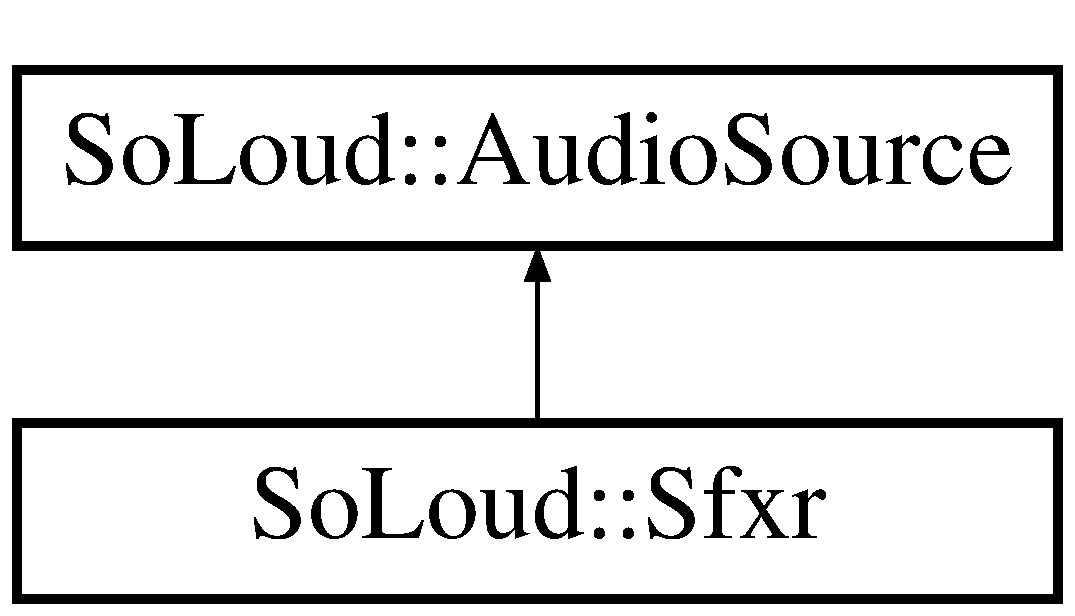
\includegraphics[height=2.000000cm]{class_so_loud_1_1_sfxr}
\end{center}
\end{figure}
\subsection*{Public Types}
\begin{DoxyCompactItemize}
\item 
\mbox{\Hypertarget{class_so_loud_1_1_sfxr_afda1c6ce4460589ccb57f2a515ad84fa}\label{class_so_loud_1_1_sfxr_afda1c6ce4460589ccb57f2a515ad84fa}} 
enum {\bfseries S\+F\+X\+R\+\_\+\+P\+R\+E\+S\+E\+TS} \{ \newline
{\bfseries C\+O\+IN}, 
{\bfseries L\+A\+S\+ER}, 
{\bfseries E\+X\+P\+L\+O\+S\+I\+ON}, 
{\bfseries P\+O\+W\+E\+R\+UP}, 
\newline
{\bfseries H\+U\+RT}, 
{\bfseries J\+U\+MP}, 
{\bfseries B\+L\+IP}
 \}
\end{DoxyCompactItemize}
\subsection*{Public Member Functions}
\begin{DoxyCompactItemize}
\item 
\mbox{\Hypertarget{class_so_loud_1_1_sfxr_a5137ecc26f9d99a11a8c5cc0a31a2b81}\label{class_so_loud_1_1_sfxr_a5137ecc26f9d99a11a8c5cc0a31a2b81}} 
void {\bfseries reset\+Params} ()
\item 
\mbox{\Hypertarget{class_so_loud_1_1_sfxr_a2f0d61ef7e75a28cb7ba3d93cce222b5}\label{class_so_loud_1_1_sfxr_a2f0d61ef7e75a28cb7ba3d93cce222b5}} 
result {\bfseries load\+Params} (const char $\ast$a\+Filename)
\item 
\mbox{\Hypertarget{class_so_loud_1_1_sfxr_a0e66c7c1fbbb13eaec6c3f69043ed84f}\label{class_so_loud_1_1_sfxr_a0e66c7c1fbbb13eaec6c3f69043ed84f}} 
result {\bfseries load\+Params\+Mem} (unsigned char $\ast$a\+Mem, unsigned int a\+Length, bool a\+Copy=false, bool a\+Take\+Ownership=true)
\item 
\mbox{\Hypertarget{class_so_loud_1_1_sfxr_a5f7e139d3456e480c4dd5e9f890d89c1}\label{class_so_loud_1_1_sfxr_a5f7e139d3456e480c4dd5e9f890d89c1}} 
result {\bfseries load\+Params\+File} (\mbox{\hyperlink{class_so_loud_1_1_file}{File}} $\ast$a\+File)
\item 
\mbox{\Hypertarget{class_so_loud_1_1_sfxr_addbf8f2b5cc1606bf6b7662057ba363a}\label{class_so_loud_1_1_sfxr_addbf8f2b5cc1606bf6b7662057ba363a}} 
result {\bfseries load\+Preset} (int a\+Preset\+No, int a\+Rand\+Seed)
\item 
\mbox{\Hypertarget{class_so_loud_1_1_sfxr_a5e6ed4e55884624a70b271ae2ef4f8df}\label{class_so_loud_1_1_sfxr_a5e6ed4e55884624a70b271ae2ef4f8df}} 
virtual \mbox{\hyperlink{class_so_loud_1_1_audio_source_instance}{Audio\+Source\+Instance}} $\ast$ {\bfseries create\+Instance} ()
\end{DoxyCompactItemize}
\subsection*{Public Attributes}
\begin{DoxyCompactItemize}
\item 
\mbox{\Hypertarget{class_so_loud_1_1_sfxr_a83a62945c9e6ee812a94c9f65e109e4e}\label{class_so_loud_1_1_sfxr_a83a62945c9e6ee812a94c9f65e109e4e}} 
\mbox{\hyperlink{struct_so_loud_1_1_sfxr_params}{Sfxr\+Params}} {\bfseries m\+Params}
\item 
\mbox{\Hypertarget{class_so_loud_1_1_sfxr_af63acb43327034d8be88d85418b86a5b}\label{class_so_loud_1_1_sfxr_af63acb43327034d8be88d85418b86a5b}} 
\mbox{\hyperlink{class_so_loud_1_1_prg}{Prg}} {\bfseries m\+Rand}
\end{DoxyCompactItemize}


The documentation for this class was generated from the following file\+:\begin{DoxyCompactItemize}
\item 
deps/\+E\+S\+A\+T/include/\+E\+S\+A\+T\+\_\+extra/soloud/soloud\+\_\+sfxr.\+h\end{DoxyCompactItemize}

\hypertarget{class_so_loud_1_1_sfxr_instance}{}\section{So\+Loud\+:\+:Sfxr\+Instance Class Reference}
\label{class_so_loud_1_1_sfxr_instance}\index{So\+Loud\+::\+Sfxr\+Instance@{So\+Loud\+::\+Sfxr\+Instance}}
Inheritance diagram for So\+Loud\+:\+:Sfxr\+Instance\+:\begin{figure}[H]
\begin{center}
\leavevmode
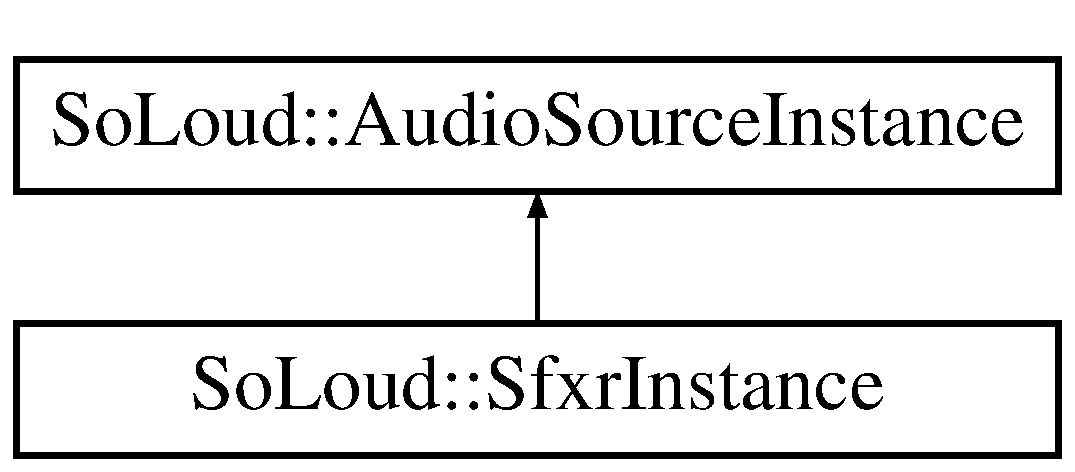
\includegraphics[height=2.000000cm]{class_so_loud_1_1_sfxr_instance}
\end{center}
\end{figure}
\subsection*{Public Member Functions}
\begin{DoxyCompactItemize}
\item 
\mbox{\Hypertarget{class_so_loud_1_1_sfxr_instance_a2308816da00b1f5f191e90c9bc97e146}\label{class_so_loud_1_1_sfxr_instance_a2308816da00b1f5f191e90c9bc97e146}} 
{\bfseries Sfxr\+Instance} (\mbox{\hyperlink{class_so_loud_1_1_sfxr}{Sfxr}} $\ast$a\+Parent)
\item 
\mbox{\Hypertarget{class_so_loud_1_1_sfxr_instance_a40f37c9ecaf740cc5a2d7c5ae760f6ca}\label{class_so_loud_1_1_sfxr_instance_a40f37c9ecaf740cc5a2d7c5ae760f6ca}} 
virtual void {\bfseries get\+Audio} (float $\ast$a\+Buffer, unsigned int a\+Samples)
\item 
\mbox{\Hypertarget{class_so_loud_1_1_sfxr_instance_ac1ca3338a70bf268384bcc89fe4a3de4}\label{class_so_loud_1_1_sfxr_instance_ac1ca3338a70bf268384bcc89fe4a3de4}} 
virtual bool {\bfseries has\+Ended} ()
\end{DoxyCompactItemize}
\subsection*{Additional Inherited Members}


The documentation for this class was generated from the following file\+:\begin{DoxyCompactItemize}
\item 
deps/\+E\+S\+A\+T/include/\+E\+S\+A\+T\+\_\+extra/soloud/soloud\+\_\+sfxr.\+h\end{DoxyCompactItemize}

\hypertarget{struct_so_loud_1_1_sfxr_params}{}\section{So\+Loud\+:\+:Sfxr\+Params Struct Reference}
\label{struct_so_loud_1_1_sfxr_params}\index{So\+Loud\+::\+Sfxr\+Params@{So\+Loud\+::\+Sfxr\+Params}}
\subsection*{Public Attributes}
\begin{DoxyCompactItemize}
\item 
\mbox{\Hypertarget{struct_so_loud_1_1_sfxr_params_acf3b1c33376a71154c1126f2b70ac464}\label{struct_so_loud_1_1_sfxr_params_acf3b1c33376a71154c1126f2b70ac464}} 
int {\bfseries wave\+\_\+type}
\item 
\mbox{\Hypertarget{struct_so_loud_1_1_sfxr_params_a8b61e1ac8b4ba33a23c96a2be75596e3}\label{struct_so_loud_1_1_sfxr_params_a8b61e1ac8b4ba33a23c96a2be75596e3}} 
float {\bfseries p\+\_\+base\+\_\+freq}
\item 
\mbox{\Hypertarget{struct_so_loud_1_1_sfxr_params_aef9a3be41efac9db3a31ed71898f684f}\label{struct_so_loud_1_1_sfxr_params_aef9a3be41efac9db3a31ed71898f684f}} 
float {\bfseries p\+\_\+freq\+\_\+limit}
\item 
\mbox{\Hypertarget{struct_so_loud_1_1_sfxr_params_a95bb6db72da1b4be65e7ed1510bf0b8b}\label{struct_so_loud_1_1_sfxr_params_a95bb6db72da1b4be65e7ed1510bf0b8b}} 
float {\bfseries p\+\_\+freq\+\_\+ramp}
\item 
\mbox{\Hypertarget{struct_so_loud_1_1_sfxr_params_aae295ff39a61937a057df41ac1b41c8b}\label{struct_so_loud_1_1_sfxr_params_aae295ff39a61937a057df41ac1b41c8b}} 
float {\bfseries p\+\_\+freq\+\_\+dramp}
\item 
\mbox{\Hypertarget{struct_so_loud_1_1_sfxr_params_a02cbcdce2fde6cdf9752ca0ad35a806f}\label{struct_so_loud_1_1_sfxr_params_a02cbcdce2fde6cdf9752ca0ad35a806f}} 
float {\bfseries p\+\_\+duty}
\item 
\mbox{\Hypertarget{struct_so_loud_1_1_sfxr_params_ac0ceb5dcbdbdd6f67fe428651c655658}\label{struct_so_loud_1_1_sfxr_params_ac0ceb5dcbdbdd6f67fe428651c655658}} 
float {\bfseries p\+\_\+duty\+\_\+ramp}
\item 
\mbox{\Hypertarget{struct_so_loud_1_1_sfxr_params_af3b6dcc8d6e55d60f137b6aa59b6860e}\label{struct_so_loud_1_1_sfxr_params_af3b6dcc8d6e55d60f137b6aa59b6860e}} 
float {\bfseries p\+\_\+vib\+\_\+strength}
\item 
\mbox{\Hypertarget{struct_so_loud_1_1_sfxr_params_a1d1205aeaac74c3b18a57f7b835eb447}\label{struct_so_loud_1_1_sfxr_params_a1d1205aeaac74c3b18a57f7b835eb447}} 
float {\bfseries p\+\_\+vib\+\_\+speed}
\item 
\mbox{\Hypertarget{struct_so_loud_1_1_sfxr_params_a419eaaa4a74133c0a74728789397242e}\label{struct_so_loud_1_1_sfxr_params_a419eaaa4a74133c0a74728789397242e}} 
float {\bfseries p\+\_\+vib\+\_\+delay}
\item 
\mbox{\Hypertarget{struct_so_loud_1_1_sfxr_params_a54e7715109ede21138595d41173586ac}\label{struct_so_loud_1_1_sfxr_params_a54e7715109ede21138595d41173586ac}} 
float {\bfseries p\+\_\+env\+\_\+attack}
\item 
\mbox{\Hypertarget{struct_so_loud_1_1_sfxr_params_a298783bdad3589b2bd92c09cd7657d3b}\label{struct_so_loud_1_1_sfxr_params_a298783bdad3589b2bd92c09cd7657d3b}} 
float {\bfseries p\+\_\+env\+\_\+sustain}
\item 
\mbox{\Hypertarget{struct_so_loud_1_1_sfxr_params_a1ec4e26d6f976b7d55b0a8afa8a889ae}\label{struct_so_loud_1_1_sfxr_params_a1ec4e26d6f976b7d55b0a8afa8a889ae}} 
float {\bfseries p\+\_\+env\+\_\+decay}
\item 
\mbox{\Hypertarget{struct_so_loud_1_1_sfxr_params_aa97a4aeb3e052afe4836089337005744}\label{struct_so_loud_1_1_sfxr_params_aa97a4aeb3e052afe4836089337005744}} 
float {\bfseries p\+\_\+env\+\_\+punch}
\item 
\mbox{\Hypertarget{struct_so_loud_1_1_sfxr_params_ae4e7d3d3cf350557cf3a31b928d19033}\label{struct_so_loud_1_1_sfxr_params_ae4e7d3d3cf350557cf3a31b928d19033}} 
bool {\bfseries filter\+\_\+on}
\item 
\mbox{\Hypertarget{struct_so_loud_1_1_sfxr_params_acd5a00384f3910ee2085c4b3718ade11}\label{struct_so_loud_1_1_sfxr_params_acd5a00384f3910ee2085c4b3718ade11}} 
float {\bfseries p\+\_\+lpf\+\_\+resonance}
\item 
\mbox{\Hypertarget{struct_so_loud_1_1_sfxr_params_a84061a1f27c6b8cadff21b9677896670}\label{struct_so_loud_1_1_sfxr_params_a84061a1f27c6b8cadff21b9677896670}} 
float {\bfseries p\+\_\+lpf\+\_\+freq}
\item 
\mbox{\Hypertarget{struct_so_loud_1_1_sfxr_params_aa8f17052b1453af87b31c693b3b16163}\label{struct_so_loud_1_1_sfxr_params_aa8f17052b1453af87b31c693b3b16163}} 
float {\bfseries p\+\_\+lpf\+\_\+ramp}
\item 
\mbox{\Hypertarget{struct_so_loud_1_1_sfxr_params_a6682a90726b9c60df4f7c3aaf1497ac7}\label{struct_so_loud_1_1_sfxr_params_a6682a90726b9c60df4f7c3aaf1497ac7}} 
float {\bfseries p\+\_\+hpf\+\_\+freq}
\item 
\mbox{\Hypertarget{struct_so_loud_1_1_sfxr_params_ac6a93a91c96054caa661ca8a69849cd3}\label{struct_so_loud_1_1_sfxr_params_ac6a93a91c96054caa661ca8a69849cd3}} 
float {\bfseries p\+\_\+hpf\+\_\+ramp}
\item 
\mbox{\Hypertarget{struct_so_loud_1_1_sfxr_params_a77407eaea01a9729edd77601935ad630}\label{struct_so_loud_1_1_sfxr_params_a77407eaea01a9729edd77601935ad630}} 
float {\bfseries p\+\_\+pha\+\_\+offset}
\item 
\mbox{\Hypertarget{struct_so_loud_1_1_sfxr_params_aaa118d49465911a42896292d5dd9d38f}\label{struct_so_loud_1_1_sfxr_params_aaa118d49465911a42896292d5dd9d38f}} 
float {\bfseries p\+\_\+pha\+\_\+ramp}
\item 
\mbox{\Hypertarget{struct_so_loud_1_1_sfxr_params_a8e264eb463bb0d54278a7523e05f92c7}\label{struct_so_loud_1_1_sfxr_params_a8e264eb463bb0d54278a7523e05f92c7}} 
float {\bfseries p\+\_\+repeat\+\_\+speed}
\item 
\mbox{\Hypertarget{struct_so_loud_1_1_sfxr_params_a818682d30a2f7f185cd21d2e162dbad5}\label{struct_so_loud_1_1_sfxr_params_a818682d30a2f7f185cd21d2e162dbad5}} 
float {\bfseries p\+\_\+arp\+\_\+speed}
\item 
\mbox{\Hypertarget{struct_so_loud_1_1_sfxr_params_a0d98f475455a59d71a3aed2092a646e5}\label{struct_so_loud_1_1_sfxr_params_a0d98f475455a59d71a3aed2092a646e5}} 
float {\bfseries p\+\_\+arp\+\_\+mod}
\item 
\mbox{\Hypertarget{struct_so_loud_1_1_sfxr_params_a914028741afd880475085953ae2872a3}\label{struct_so_loud_1_1_sfxr_params_a914028741afd880475085953ae2872a3}} 
float {\bfseries master\+\_\+vol}
\item 
\mbox{\Hypertarget{struct_so_loud_1_1_sfxr_params_aa0ed234579b29fa59b923f3ee0849761}\label{struct_so_loud_1_1_sfxr_params_aa0ed234579b29fa59b923f3ee0849761}} 
float {\bfseries sound\+\_\+vol}
\end{DoxyCompactItemize}


The documentation for this struct was generated from the following file\+:\begin{DoxyCompactItemize}
\item 
deps/\+E\+S\+A\+T/include/\+E\+S\+A\+T\+\_\+extra/soloud/soloud\+\_\+sfxr.\+h\end{DoxyCompactItemize}

\hypertarget{structtinyobj_1_1shape__t}{}\section{tinyobj\+:\+:shape\+\_\+t Struct Reference}
\label{structtinyobj_1_1shape__t}\index{tinyobj\+::shape\+\_\+t@{tinyobj\+::shape\+\_\+t}}
\subsection*{Public Attributes}
\begin{DoxyCompactItemize}
\item 
\mbox{\Hypertarget{structtinyobj_1_1shape__t_a98650e2e66d00934f68de88eafb34630}\label{structtinyobj_1_1shape__t_a98650e2e66d00934f68de88eafb34630}} 
std\+::string {\bfseries name}
\item 
\mbox{\Hypertarget{structtinyobj_1_1shape__t_a3dacb06dfbfe9e245ff4bc7b5b3d9818}\label{structtinyobj_1_1shape__t_a3dacb06dfbfe9e245ff4bc7b5b3d9818}} 
\mbox{\hyperlink{structtinyobj_1_1mesh__t}{mesh\+\_\+t}} {\bfseries mesh}
\end{DoxyCompactItemize}


The documentation for this struct was generated from the following file\+:\begin{DoxyCompactItemize}
\item 
deps/\+E\+S\+A\+T/include/\+E\+S\+A\+T\+\_\+extra/tiny\+\_\+obj\+\_\+loader.\+h\end{DoxyCompactItemize}

\hypertarget{class_so_loud_1_1_soloud}{}\section{So\+Loud\+:\+:Soloud Class Reference}
\label{class_so_loud_1_1_soloud}\index{So\+Loud\+::\+Soloud@{So\+Loud\+::\+Soloud}}
\subsection*{Public Types}
\begin{DoxyCompactItemize}
\item 
\mbox{\Hypertarget{class_so_loud_1_1_soloud_ac96d355c9a04c9bccb5540ff93555264}\label{class_so_loud_1_1_soloud_ac96d355c9a04c9bccb5540ff93555264}} 
enum {\bfseries B\+A\+C\+K\+E\+N\+DS} \{ \newline
{\bfseries A\+U\+TO} = 0, 
{\bfseries S\+DL}, 
{\bfseries S\+D\+L2}, 
{\bfseries P\+O\+R\+T\+A\+U\+D\+IO}, 
\newline
{\bfseries W\+I\+N\+MM}, 
{\bfseries X\+A\+U\+D\+I\+O2}, 
{\bfseries W\+A\+S\+A\+PI}, 
{\bfseries A\+L\+SA}, 
\newline
{\bfseries O\+SS}, 
{\bfseries O\+P\+E\+N\+AL}, 
{\bfseries C\+O\+R\+E\+A\+U\+D\+IO}, 
{\bfseries O\+P\+E\+N\+S\+L\+ES}, 
\newline
{\bfseries N\+U\+L\+L\+D\+R\+I\+V\+ER}, 
{\bfseries B\+A\+C\+K\+E\+N\+D\+\_\+\+M\+AX}
 \}
\item 
\mbox{\Hypertarget{class_so_loud_1_1_soloud_ae53f6fced10211ed39249c59bd24ad6b}\label{class_so_loud_1_1_soloud_ae53f6fced10211ed39249c59bd24ad6b}} 
enum {\bfseries F\+L\+A\+GS} \{ {\bfseries C\+L\+I\+P\+\_\+\+R\+O\+U\+N\+D\+O\+FF} = 1, 
{\bfseries E\+N\+A\+B\+L\+E\+\_\+\+V\+I\+S\+U\+A\+L\+I\+Z\+A\+T\+I\+ON} = 2, 
{\bfseries L\+E\+F\+T\+\_\+\+H\+A\+N\+D\+E\+D\+\_\+3D} = 4
 \}
\end{DoxyCompactItemize}
\subsection*{Public Member Functions}
\begin{DoxyCompactItemize}
\item 
\mbox{\Hypertarget{class_so_loud_1_1_soloud_ad0d7e608a0607aa4f82382c48210058a}\label{class_so_loud_1_1_soloud_ad0d7e608a0607aa4f82382c48210058a}} 
result {\bfseries init} (unsigned int a\+Flags=Soloud\+::\+C\+L\+I\+P\+\_\+\+R\+O\+U\+N\+D\+O\+FF, unsigned int a\+Backend=Soloud\+::\+A\+U\+TO, unsigned int a\+Samplerate=Soloud\+::\+A\+U\+TO, unsigned int a\+Buffer\+Size=Soloud\+::\+A\+U\+TO, unsigned int a\+Channels=2)
\item 
\mbox{\Hypertarget{class_so_loud_1_1_soloud_a4a9787e28373943fbf75b91eeb49e39d}\label{class_so_loud_1_1_soloud_a4a9787e28373943fbf75b91eeb49e39d}} 
void {\bfseries deinit} ()
\item 
\mbox{\Hypertarget{class_so_loud_1_1_soloud_ad20993bd06c7bbd73cf841b322b5f4d8}\label{class_so_loud_1_1_soloud_ad20993bd06c7bbd73cf841b322b5f4d8}} 
unsigned int {\bfseries get\+Version} () const
\item 
\mbox{\Hypertarget{class_so_loud_1_1_soloud_a33c20c08430f9906dc75bedcfc9f11b9}\label{class_so_loud_1_1_soloud_a33c20c08430f9906dc75bedcfc9f11b9}} 
const char $\ast$ {\bfseries get\+Error\+String} (result a\+Error\+Code) const
\item 
\mbox{\Hypertarget{class_so_loud_1_1_soloud_a1db83b486cbf00062b267c3cdaca6f1a}\label{class_so_loud_1_1_soloud_a1db83b486cbf00062b267c3cdaca6f1a}} 
unsigned int {\bfseries get\+Backend\+Id} ()
\item 
\mbox{\Hypertarget{class_so_loud_1_1_soloud_a16e56871e5ce01ec8202d4a95d917513}\label{class_so_loud_1_1_soloud_a16e56871e5ce01ec8202d4a95d917513}} 
const char $\ast$ {\bfseries get\+Backend\+String} ()
\item 
\mbox{\Hypertarget{class_so_loud_1_1_soloud_afe47adf7d9009bedc71265bf97e1ffd6}\label{class_so_loud_1_1_soloud_afe47adf7d9009bedc71265bf97e1ffd6}} 
unsigned int {\bfseries get\+Backend\+Channels} ()
\item 
\mbox{\Hypertarget{class_so_loud_1_1_soloud_a1e8cd90a27fc3f1cc9e3b2fc414750fe}\label{class_so_loud_1_1_soloud_a1e8cd90a27fc3f1cc9e3b2fc414750fe}} 
unsigned int {\bfseries get\+Backend\+Samplerate} ()
\item 
\mbox{\Hypertarget{class_so_loud_1_1_soloud_a0dcf47a9f712d0bb693cff85ca8683cd}\label{class_so_loud_1_1_soloud_a0dcf47a9f712d0bb693cff85ca8683cd}} 
unsigned int {\bfseries get\+Backend\+Buffer\+Size} ()
\item 
\mbox{\Hypertarget{class_so_loud_1_1_soloud_a1835694c29ac4ce0ea9e4bcaf7ef3373}\label{class_so_loud_1_1_soloud_a1835694c29ac4ce0ea9e4bcaf7ef3373}} 
result {\bfseries set\+Speaker\+Position} (unsigned int a\+Channel, float aX, float aY, float aZ)
\item 
\mbox{\Hypertarget{class_so_loud_1_1_soloud_abd8f5c6c7f1ee00ed340d09302448a9a}\label{class_so_loud_1_1_soloud_abd8f5c6c7f1ee00ed340d09302448a9a}} 
handle {\bfseries play} (\mbox{\hyperlink{class_so_loud_1_1_audio_source}{Audio\+Source}} \&a\+Sound, float a\+Volume=-\/1.\+0f, float a\+Pan=0.\+0f, bool a\+Paused=0, unsigned int a\+Bus=0)
\item 
\mbox{\Hypertarget{class_so_loud_1_1_soloud_a371446b6bf287a9e10514dd9b113111b}\label{class_so_loud_1_1_soloud_a371446b6bf287a9e10514dd9b113111b}} 
handle {\bfseries play\+Clocked} (time a\+Sound\+Time, \mbox{\hyperlink{class_so_loud_1_1_audio_source}{Audio\+Source}} \&a\+Sound, float a\+Volume=-\/1.\+0f, float a\+Pan=0.\+0f, unsigned int a\+Bus=0)
\item 
\mbox{\Hypertarget{class_so_loud_1_1_soloud_aec0c42f795c8213606ce885c45d9e4e8}\label{class_so_loud_1_1_soloud_aec0c42f795c8213606ce885c45d9e4e8}} 
handle {\bfseries play3d} (\mbox{\hyperlink{class_so_loud_1_1_audio_source}{Audio\+Source}} \&a\+Sound, float a\+PosX, float a\+PosY, float a\+PosZ, float a\+VelX=0.\+0f, float a\+Vel\+Y=0.\+0f, float a\+Vel\+Z=0.\+0f, float a\+Volume=1.\+0f, bool a\+Paused=0, unsigned int a\+Bus=0)
\item 
\mbox{\Hypertarget{class_so_loud_1_1_soloud_a5d1e394c21dc42b8e6f0a1e6a827228c}\label{class_so_loud_1_1_soloud_a5d1e394c21dc42b8e6f0a1e6a827228c}} 
handle {\bfseries play3d\+Clocked} (time a\+Sound\+Time, \mbox{\hyperlink{class_so_loud_1_1_audio_source}{Audio\+Source}} \&a\+Sound, float a\+PosX, float a\+PosY, float a\+PosZ, float a\+VelX=0.\+0f, float a\+Vel\+Y=0.\+0f, float a\+Vel\+Z=0.\+0f, float a\+Volume=1.\+0f, unsigned int a\+Bus=0)
\item 
\mbox{\Hypertarget{class_so_loud_1_1_soloud_afef203ec579c25b59d9d2bc83692d7cc}\label{class_so_loud_1_1_soloud_afef203ec579c25b59d9d2bc83692d7cc}} 
void {\bfseries seek} (handle a\+Voice\+Handle, time a\+Seconds)
\item 
\mbox{\Hypertarget{class_so_loud_1_1_soloud_a04712e8863bb2a1078251f91d4a6d776}\label{class_so_loud_1_1_soloud_a04712e8863bb2a1078251f91d4a6d776}} 
void {\bfseries stop} (handle a\+Voice\+Handle)
\item 
\mbox{\Hypertarget{class_so_loud_1_1_soloud_ab1fa4f692ae99cc1fac597d67958c1ce}\label{class_so_loud_1_1_soloud_ab1fa4f692ae99cc1fac597d67958c1ce}} 
void {\bfseries stop\+All} ()
\item 
\mbox{\Hypertarget{class_so_loud_1_1_soloud_ab0079b4ee6360bceff408df9c2bee634}\label{class_so_loud_1_1_soloud_ab0079b4ee6360bceff408df9c2bee634}} 
void {\bfseries stop\+Audio\+Source} (\mbox{\hyperlink{class_so_loud_1_1_audio_source}{Audio\+Source}} \&a\+Sound)
\item 
\mbox{\Hypertarget{class_so_loud_1_1_soloud_af9871d1329e2d5613d99ff34c17e1ea2}\label{class_so_loud_1_1_soloud_af9871d1329e2d5613d99ff34c17e1ea2}} 
void {\bfseries set\+Filter\+Parameter} (handle a\+Voice\+Handle, unsigned int a\+Filter\+Id, unsigned int a\+Attribute\+Id, float a\+Value)
\item 
\mbox{\Hypertarget{class_so_loud_1_1_soloud_a83072ac27d31de55084c6160eecfa72f}\label{class_so_loud_1_1_soloud_a83072ac27d31de55084c6160eecfa72f}} 
float {\bfseries get\+Filter\+Parameter} (handle a\+Voice\+Handle, unsigned int a\+Filter\+Id, unsigned int a\+Attribute\+Id)
\item 
\mbox{\Hypertarget{class_so_loud_1_1_soloud_a342a6968934617d9b38fa380f9dbf512}\label{class_so_loud_1_1_soloud_a342a6968934617d9b38fa380f9dbf512}} 
void {\bfseries fade\+Filter\+Parameter} (handle a\+Voice\+Handle, unsigned int a\+Filter\+Id, unsigned int a\+Attribute\+Id, float a\+To, time a\+Time)
\item 
\mbox{\Hypertarget{class_so_loud_1_1_soloud_ab422df9ba2b61c6453347ee99307b490}\label{class_so_loud_1_1_soloud_ab422df9ba2b61c6453347ee99307b490}} 
void {\bfseries oscillate\+Filter\+Parameter} (handle a\+Voice\+Handle, unsigned int a\+Filter\+Id, unsigned int a\+Attribute\+Id, float a\+From, float a\+To, time a\+Time)
\item 
\mbox{\Hypertarget{class_so_loud_1_1_soloud_a86cd9de7f52d7a0fa3f59e840a914d1e}\label{class_so_loud_1_1_soloud_a86cd9de7f52d7a0fa3f59e840a914d1e}} 
time {\bfseries get\+Stream\+Time} (handle a\+Voice\+Handle)
\item 
\mbox{\Hypertarget{class_so_loud_1_1_soloud_a01f9dbaf2cde0de348936d8ff0761de6}\label{class_so_loud_1_1_soloud_a01f9dbaf2cde0de348936d8ff0761de6}} 
bool {\bfseries get\+Pause} (handle a\+Voice\+Handle)
\item 
\mbox{\Hypertarget{class_so_loud_1_1_soloud_a6aea2e6c7619dbcb087cd2536560498d}\label{class_so_loud_1_1_soloud_a6aea2e6c7619dbcb087cd2536560498d}} 
float {\bfseries get\+Volume} (handle a\+Voice\+Handle)
\item 
\mbox{\Hypertarget{class_so_loud_1_1_soloud_ae4d5eb33002809502ecb41fd12e9532d}\label{class_so_loud_1_1_soloud_ae4d5eb33002809502ecb41fd12e9532d}} 
float {\bfseries get\+Overall\+Volume} (handle a\+Voice\+Handle)
\item 
\mbox{\Hypertarget{class_so_loud_1_1_soloud_a9da54ea4e9d272f164e3229a30025b1b}\label{class_so_loud_1_1_soloud_a9da54ea4e9d272f164e3229a30025b1b}} 
float {\bfseries get\+Pan} (handle a\+Voice\+Handle)
\item 
\mbox{\Hypertarget{class_so_loud_1_1_soloud_a0fb66756e447a46acc4716cb49622d7f}\label{class_so_loud_1_1_soloud_a0fb66756e447a46acc4716cb49622d7f}} 
float {\bfseries get\+Samplerate} (handle a\+Voice\+Handle)
\item 
\mbox{\Hypertarget{class_so_loud_1_1_soloud_a92fede186fb8d7be97be8b8138fa7c2e}\label{class_so_loud_1_1_soloud_a92fede186fb8d7be97be8b8138fa7c2e}} 
bool {\bfseries get\+Protect\+Voice} (handle a\+Voice\+Handle)
\item 
\mbox{\Hypertarget{class_so_loud_1_1_soloud_a11dc6c58de0c215580afca91d4db4fe6}\label{class_so_loud_1_1_soloud_a11dc6c58de0c215580afca91d4db4fe6}} 
unsigned int {\bfseries get\+Active\+Voice\+Count} ()
\item 
\mbox{\Hypertarget{class_so_loud_1_1_soloud_aec874424a3cb96d57b4c00b29c7deec4}\label{class_so_loud_1_1_soloud_aec874424a3cb96d57b4c00b29c7deec4}} 
unsigned int {\bfseries get\+Voice\+Count} ()
\item 
\mbox{\Hypertarget{class_so_loud_1_1_soloud_a94e95f482541930fc49aec27f8fc6cc9}\label{class_so_loud_1_1_soloud_a94e95f482541930fc49aec27f8fc6cc9}} 
bool {\bfseries is\+Valid\+Voice\+Handle} (handle a\+Voice\+Handle)
\item 
\mbox{\Hypertarget{class_so_loud_1_1_soloud_a648e056e53c2b191394408d61d3c72e4}\label{class_so_loud_1_1_soloud_a648e056e53c2b191394408d61d3c72e4}} 
float {\bfseries get\+Relative\+Play\+Speed} (handle a\+Voice\+Handle)
\item 
\mbox{\Hypertarget{class_so_loud_1_1_soloud_a5a9ae5c588a41b7c88056ed160969866}\label{class_so_loud_1_1_soloud_a5a9ae5c588a41b7c88056ed160969866}} 
float {\bfseries get\+Post\+Clip\+Scaler} () const
\item 
\mbox{\Hypertarget{class_so_loud_1_1_soloud_ae3d3f2e14082b41d5160c0d291d0bb79}\label{class_so_loud_1_1_soloud_ae3d3f2e14082b41d5160c0d291d0bb79}} 
float {\bfseries get\+Global\+Volume} () const
\item 
\mbox{\Hypertarget{class_so_loud_1_1_soloud_a564c5101270995c1410016b8d53a982a}\label{class_so_loud_1_1_soloud_a564c5101270995c1410016b8d53a982a}} 
unsigned int {\bfseries get\+Max\+Active\+Voice\+Count} () const
\item 
\mbox{\Hypertarget{class_so_loud_1_1_soloud_a0d28a9886c1d1dc7389ad12fe893d8ed}\label{class_so_loud_1_1_soloud_a0d28a9886c1d1dc7389ad12fe893d8ed}} 
bool {\bfseries get\+Looping} (handle a\+Voice\+Handle)
\item 
\mbox{\Hypertarget{class_so_loud_1_1_soloud_aabf12bbd4289f96ca0b80ab5f36561d1}\label{class_so_loud_1_1_soloud_aabf12bbd4289f96ca0b80ab5f36561d1}} 
void {\bfseries set\+Looping} (handle a\+Voice\+Handle, bool a\+Looping)
\item 
\mbox{\Hypertarget{class_so_loud_1_1_soloud_ad8249efec6260ec8fabdce1202255cca}\label{class_so_loud_1_1_soloud_ad8249efec6260ec8fabdce1202255cca}} 
result {\bfseries set\+Max\+Active\+Voice\+Count} (unsigned int a\+Voice\+Count)
\item 
\mbox{\Hypertarget{class_so_loud_1_1_soloud_a637327d28bfba8c649cd1055b1b589b1}\label{class_so_loud_1_1_soloud_a637327d28bfba8c649cd1055b1b589b1}} 
void {\bfseries set\+Inaudible\+Behavior} (handle a\+Voice\+Handle, bool a\+Must\+Tick, bool a\+Kill)
\item 
\mbox{\Hypertarget{class_so_loud_1_1_soloud_a685ac512e992520cd939460308ef90f9}\label{class_so_loud_1_1_soloud_a685ac512e992520cd939460308ef90f9}} 
void {\bfseries set\+Global\+Volume} (float a\+Volume)
\item 
\mbox{\Hypertarget{class_so_loud_1_1_soloud_a66ddc86d64a1a1afe0e3ee729f03137e}\label{class_so_loud_1_1_soloud_a66ddc86d64a1a1afe0e3ee729f03137e}} 
void {\bfseries set\+Post\+Clip\+Scaler} (float a\+Scaler)
\item 
\mbox{\Hypertarget{class_so_loud_1_1_soloud_a950ec356b2fabceaa35b8a7eb03cf4d3}\label{class_so_loud_1_1_soloud_a950ec356b2fabceaa35b8a7eb03cf4d3}} 
void {\bfseries set\+Pause} (handle a\+Voice\+Handle, bool a\+Pause)
\item 
\mbox{\Hypertarget{class_so_loud_1_1_soloud_a6e88cde01e539557fcfe3afbe9d9ef09}\label{class_so_loud_1_1_soloud_a6e88cde01e539557fcfe3afbe9d9ef09}} 
void {\bfseries set\+Pause\+All} (bool a\+Pause)
\item 
\mbox{\Hypertarget{class_so_loud_1_1_soloud_a45ac9d70d52266fb60651b0f4642d7cb}\label{class_so_loud_1_1_soloud_a45ac9d70d52266fb60651b0f4642d7cb}} 
result {\bfseries set\+Relative\+Play\+Speed} (handle a\+Voice\+Handle, float a\+Speed)
\item 
\mbox{\Hypertarget{class_so_loud_1_1_soloud_affa0f7f149a859bca79deb55b0c66e5c}\label{class_so_loud_1_1_soloud_affa0f7f149a859bca79deb55b0c66e5c}} 
void {\bfseries set\+Protect\+Voice} (handle a\+Voice\+Handle, bool a\+Protect)
\item 
\mbox{\Hypertarget{class_so_loud_1_1_soloud_a1a6e400c35e543ed70c7be3ae808b4da}\label{class_so_loud_1_1_soloud_a1a6e400c35e543ed70c7be3ae808b4da}} 
void {\bfseries set\+Samplerate} (handle a\+Voice\+Handle, float a\+Samplerate)
\item 
\mbox{\Hypertarget{class_so_loud_1_1_soloud_a2c78e611871ef145b976a5c717c8d865}\label{class_so_loud_1_1_soloud_a2c78e611871ef145b976a5c717c8d865}} 
void {\bfseries set\+Pan} (handle a\+Voice\+Handle, float a\+Pan)
\item 
\mbox{\Hypertarget{class_so_loud_1_1_soloud_a31b07a9d4c8ff56adaf397586a7483a8}\label{class_so_loud_1_1_soloud_a31b07a9d4c8ff56adaf397586a7483a8}} 
void {\bfseries set\+Pan\+Absolute} (handle a\+Voice\+Handle, float a\+L\+Volume, float a\+R\+Volume, float a\+L\+B\+Volume=0, float a\+R\+B\+Volume=0, float a\+C\+Volume=0, float a\+S\+Volume=0)
\item 
\mbox{\Hypertarget{class_so_loud_1_1_soloud_a1e6f5c43489244f0d6495845a310508c}\label{class_so_loud_1_1_soloud_a1e6f5c43489244f0d6495845a310508c}} 
void {\bfseries set\+Volume} (handle a\+Voice\+Handle, float a\+Volume)
\item 
\mbox{\Hypertarget{class_so_loud_1_1_soloud_a009c703c8db214d6452b77456f57b56a}\label{class_so_loud_1_1_soloud_a009c703c8db214d6452b77456f57b56a}} 
void {\bfseries set\+Delay\+Samples} (handle a\+Voice\+Handle, unsigned int a\+Samples)
\item 
\mbox{\Hypertarget{class_so_loud_1_1_soloud_af6ac66de9742499dd616de099758f344}\label{class_so_loud_1_1_soloud_af6ac66de9742499dd616de099758f344}} 
void {\bfseries fade\+Volume} (handle a\+Voice\+Handle, float a\+To, time a\+Time)
\item 
\mbox{\Hypertarget{class_so_loud_1_1_soloud_aaac0c9adda71d06262455b78dea8d965}\label{class_so_loud_1_1_soloud_aaac0c9adda71d06262455b78dea8d965}} 
void {\bfseries fade\+Pan} (handle a\+Voice\+Handle, float a\+To, time a\+Time)
\item 
\mbox{\Hypertarget{class_so_loud_1_1_soloud_aa056f4f17f729fe00db005b5ecc4b565}\label{class_so_loud_1_1_soloud_aa056f4f17f729fe00db005b5ecc4b565}} 
void {\bfseries fade\+Relative\+Play\+Speed} (handle a\+Voice\+Handle, float a\+To, time a\+Time)
\item 
\mbox{\Hypertarget{class_so_loud_1_1_soloud_a4722c8b333f053aa5e41f73283cadfad}\label{class_so_loud_1_1_soloud_a4722c8b333f053aa5e41f73283cadfad}} 
void {\bfseries fade\+Global\+Volume} (float a\+To, time a\+Time)
\item 
\mbox{\Hypertarget{class_so_loud_1_1_soloud_aafbb714419cbf0ac4cbc14c06aaf3fd7}\label{class_so_loud_1_1_soloud_aafbb714419cbf0ac4cbc14c06aaf3fd7}} 
void {\bfseries schedule\+Pause} (handle a\+Voice\+Handle, time a\+Time)
\item 
\mbox{\Hypertarget{class_so_loud_1_1_soloud_a00c9b4715e18143d3f13ae9c42d2ae45}\label{class_so_loud_1_1_soloud_a00c9b4715e18143d3f13ae9c42d2ae45}} 
void {\bfseries schedule\+Stop} (handle a\+Voice\+Handle, time a\+Time)
\item 
\mbox{\Hypertarget{class_so_loud_1_1_soloud_a260cb4446fc97249cfd9c353020bfafa}\label{class_so_loud_1_1_soloud_a260cb4446fc97249cfd9c353020bfafa}} 
void {\bfseries oscillate\+Volume} (handle a\+Voice\+Handle, float a\+From, float a\+To, time a\+Time)
\item 
\mbox{\Hypertarget{class_so_loud_1_1_soloud_aa8843cec3f6cfff5a3e6652f890e470e}\label{class_so_loud_1_1_soloud_aa8843cec3f6cfff5a3e6652f890e470e}} 
void {\bfseries oscillate\+Pan} (handle a\+Voice\+Handle, float a\+From, float a\+To, time a\+Time)
\item 
\mbox{\Hypertarget{class_so_loud_1_1_soloud_a9ad9542bc726a315b130b40916b095a0}\label{class_so_loud_1_1_soloud_a9ad9542bc726a315b130b40916b095a0}} 
void {\bfseries oscillate\+Relative\+Play\+Speed} (handle a\+Voice\+Handle, float a\+From, float a\+To, time a\+Time)
\item 
\mbox{\Hypertarget{class_so_loud_1_1_soloud_ae91d826c1d8ba64dbf395fe9c679a82e}\label{class_so_loud_1_1_soloud_ae91d826c1d8ba64dbf395fe9c679a82e}} 
void {\bfseries oscillate\+Global\+Volume} (float a\+From, float a\+To, time a\+Time)
\item 
\mbox{\Hypertarget{class_so_loud_1_1_soloud_a7a357dd58112d34becacfa100d6b7a19}\label{class_so_loud_1_1_soloud_a7a357dd58112d34becacfa100d6b7a19}} 
void {\bfseries set\+Global\+Filter} (unsigned int a\+Filter\+Id, \mbox{\hyperlink{class_so_loud_1_1_filter}{Filter}} $\ast$a\+Filter)
\item 
\mbox{\Hypertarget{class_so_loud_1_1_soloud_a291ec9f5539cd530b6eec30ec83155b4}\label{class_so_loud_1_1_soloud_a291ec9f5539cd530b6eec30ec83155b4}} 
void {\bfseries set\+Visualization\+Enable} (bool a\+Enable)
\item 
\mbox{\Hypertarget{class_so_loud_1_1_soloud_a177bd43443be97f8b372ec03d2c76ec9}\label{class_so_loud_1_1_soloud_a177bd43443be97f8b372ec03d2c76ec9}} 
float $\ast$ {\bfseries calc\+F\+FT} ()
\item 
\mbox{\Hypertarget{class_so_loud_1_1_soloud_a20d80a4165eac224db098eef2e91c235}\label{class_so_loud_1_1_soloud_a20d80a4165eac224db098eef2e91c235}} 
float $\ast$ {\bfseries get\+Wave} ()
\item 
\mbox{\Hypertarget{class_so_loud_1_1_soloud_a52f6f46f7ae7336142b513ae9fb85d8a}\label{class_so_loud_1_1_soloud_a52f6f46f7ae7336142b513ae9fb85d8a}} 
unsigned int {\bfseries get\+Loop\+Count} (handle a\+Voice\+Handle)
\item 
\mbox{\Hypertarget{class_so_loud_1_1_soloud_a6d3e22a24f49a86edce0ad542d9656bb}\label{class_so_loud_1_1_soloud_a6d3e22a24f49a86edce0ad542d9656bb}} 
float {\bfseries get\+Info} (handle a\+Voice\+Handle, unsigned int a\+Info\+Key)
\item 
\mbox{\Hypertarget{class_so_loud_1_1_soloud_aeb0fd120e6e0239c9e718fb8789ddffe}\label{class_so_loud_1_1_soloud_aeb0fd120e6e0239c9e718fb8789ddffe}} 
handle {\bfseries create\+Voice\+Group} ()
\item 
\mbox{\Hypertarget{class_so_loud_1_1_soloud_aae50bbfa2f6bd1e598ef6b5b15636e9c}\label{class_so_loud_1_1_soloud_aae50bbfa2f6bd1e598ef6b5b15636e9c}} 
result {\bfseries destroy\+Voice\+Group} (handle a\+Voice\+Group\+Handle)
\item 
\mbox{\Hypertarget{class_so_loud_1_1_soloud_a9db61d9832918e34b27fc8f07e03181a}\label{class_so_loud_1_1_soloud_a9db61d9832918e34b27fc8f07e03181a}} 
result {\bfseries add\+Voice\+To\+Group} (handle a\+Voice\+Group\+Handle, handle a\+Voice\+Handle)
\item 
\mbox{\Hypertarget{class_so_loud_1_1_soloud_a7e0cce56db2108f4401244a7f7b4b209}\label{class_so_loud_1_1_soloud_a7e0cce56db2108f4401244a7f7b4b209}} 
bool {\bfseries is\+Voice\+Group} (handle a\+Voice\+Group\+Handle)
\item 
\mbox{\Hypertarget{class_so_loud_1_1_soloud_af7805b0b20fc49629a9e45eda96ae445}\label{class_so_loud_1_1_soloud_af7805b0b20fc49629a9e45eda96ae445}} 
bool {\bfseries is\+Voice\+Group\+Empty} (handle a\+Voice\+Group\+Handle)
\item 
\mbox{\Hypertarget{class_so_loud_1_1_soloud_a21eb58ebde3955245ac69e3aa5b5f145}\label{class_so_loud_1_1_soloud_a21eb58ebde3955245ac69e3aa5b5f145}} 
void {\bfseries update3d\+Audio} ()
\item 
\mbox{\Hypertarget{class_so_loud_1_1_soloud_a0e819643ca149ca31718322cdde5bf00}\label{class_so_loud_1_1_soloud_a0e819643ca149ca31718322cdde5bf00}} 
result {\bfseries set3d\+Sound\+Speed} (float a\+Speed)
\item 
\mbox{\Hypertarget{class_so_loud_1_1_soloud_a49769664474746f5eada52300e46f2b8}\label{class_so_loud_1_1_soloud_a49769664474746f5eada52300e46f2b8}} 
float {\bfseries get3d\+Sound\+Speed} ()
\item 
\mbox{\Hypertarget{class_so_loud_1_1_soloud_a3f2bfc85ad456ba9987fdb6d2ea6497b}\label{class_so_loud_1_1_soloud_a3f2bfc85ad456ba9987fdb6d2ea6497b}} 
void {\bfseries set3d\+Listener\+Parameters} (float a\+PosX, float a\+PosY, float a\+PosZ, float a\+AtX, float a\+AtY, float a\+AtZ, float a\+UpX, float a\+UpY, float a\+UpZ, float a\+VelocityX=0.\+0f, float a\+Velocity\+Y=0.\+0f, float a\+Velocity\+Z=0.\+0f)
\item 
\mbox{\Hypertarget{class_so_loud_1_1_soloud_a2a26c92f8ba7b283da730d038ca07ab5}\label{class_so_loud_1_1_soloud_a2a26c92f8ba7b283da730d038ca07ab5}} 
void {\bfseries set3d\+Listener\+Position} (float a\+PosX, float a\+PosY, float a\+PosZ)
\item 
\mbox{\Hypertarget{class_so_loud_1_1_soloud_aeb3d87e784043242e8a36003a1b5a1d5}\label{class_so_loud_1_1_soloud_aeb3d87e784043242e8a36003a1b5a1d5}} 
void {\bfseries set3d\+Listener\+At} (float a\+AtX, float a\+AtY, float a\+AtZ)
\item 
\mbox{\Hypertarget{class_so_loud_1_1_soloud_a73d76cc9ab22a2179eb0f6b463b6744a}\label{class_so_loud_1_1_soloud_a73d76cc9ab22a2179eb0f6b463b6744a}} 
void {\bfseries set3d\+Listener\+Up} (float a\+UpX, float a\+UpY, float a\+UpZ)
\item 
\mbox{\Hypertarget{class_so_loud_1_1_soloud_acaa3d925bc946965e8320ad9b50ea34e}\label{class_so_loud_1_1_soloud_acaa3d925bc946965e8320ad9b50ea34e}} 
void {\bfseries set3d\+Listener\+Velocity} (float a\+VelocityX, float a\+VelocityY, float a\+VelocityZ)
\item 
\mbox{\Hypertarget{class_so_loud_1_1_soloud_a3be0dac0ceb4d9580fec048746ed789b}\label{class_so_loud_1_1_soloud_a3be0dac0ceb4d9580fec048746ed789b}} 
void {\bfseries set3d\+Source\+Parameters} (handle a\+Voice\+Handle, float a\+PosX, float a\+PosY, float a\+PosZ, float a\+VelocityX=0.\+0f, float a\+Velocity\+Y=0.\+0f, float a\+Velocity\+Z=0.\+0f)
\item 
\mbox{\Hypertarget{class_so_loud_1_1_soloud_ac1f8eeab636353cccafdabf026495ccd}\label{class_so_loud_1_1_soloud_ac1f8eeab636353cccafdabf026495ccd}} 
void {\bfseries set3d\+Source\+Position} (handle a\+Voice\+Handle, float a\+PosX, float a\+PosY, float a\+PosZ)
\item 
\mbox{\Hypertarget{class_so_loud_1_1_soloud_a367f584ad9e792a1042b1aa1ed02ad49}\label{class_so_loud_1_1_soloud_a367f584ad9e792a1042b1aa1ed02ad49}} 
void {\bfseries set3d\+Source\+Velocity} (handle a\+Voice\+Handle, float a\+VelocityX, float a\+VelocityY, float a\+VelocityZ)
\item 
\mbox{\Hypertarget{class_so_loud_1_1_soloud_a16f6e9dc7eed886e42d3062e04615fd1}\label{class_so_loud_1_1_soloud_a16f6e9dc7eed886e42d3062e04615fd1}} 
void {\bfseries set3d\+Source\+Min\+Max\+Distance} (handle a\+Voice\+Handle, float a\+Min\+Distance, float a\+Max\+Distance)
\item 
\mbox{\Hypertarget{class_so_loud_1_1_soloud_afa03763fb26028520a0fd4af529a0aa0}\label{class_so_loud_1_1_soloud_afa03763fb26028520a0fd4af529a0aa0}} 
void {\bfseries set3d\+Source\+Attenuation} (handle a\+Voice\+Handle, unsigned int a\+Attenuation\+Model, float a\+Attenuation\+Rolloff\+Factor)
\item 
\mbox{\Hypertarget{class_so_loud_1_1_soloud_a9909a030c0a5965bd99a8d3b3751783f}\label{class_so_loud_1_1_soloud_a9909a030c0a5965bd99a8d3b3751783f}} 
void {\bfseries set3d\+Source\+Doppler\+Factor} (handle a\+Voice\+Handle, float a\+Doppler\+Factor)
\item 
\mbox{\Hypertarget{class_so_loud_1_1_soloud_a2979c68d9d6378463821563f2d8269e9}\label{class_so_loud_1_1_soloud_a2979c68d9d6378463821563f2d8269e9}} 
void {\bfseries mix} (float $\ast$a\+Buffer, unsigned int a\+Samples)
\item 
\mbox{\Hypertarget{class_so_loud_1_1_soloud_ae7aab6e58183f9d5f109e6386ff2f449}\label{class_so_loud_1_1_soloud_ae7aab6e58183f9d5f109e6386ff2f449}} 
void {\bfseries mix\+Signed16} (short $\ast$a\+Buffer, unsigned int a\+Samples)
\item 
\mbox{\Hypertarget{class_so_loud_1_1_soloud_af89412fb8b19db246b56eb017e75bc4a}\label{class_so_loud_1_1_soloud_af89412fb8b19db246b56eb017e75bc4a}} 
void {\bfseries mix\+\_\+internal} (unsigned int a\+Samples)
\item 
\mbox{\Hypertarget{class_so_loud_1_1_soloud_a2fdc5f40776decff79e8d069ba63d308}\label{class_so_loud_1_1_soloud_a2fdc5f40776decff79e8d069ba63d308}} 
void {\bfseries postinit} (unsigned int a\+Samplerate, unsigned int a\+Buffer\+Size, unsigned int a\+Flags, unsigned int a\+Channels)
\item 
\mbox{\Hypertarget{class_so_loud_1_1_soloud_ad504d7bf238588fa6d37d464d2c1124e}\label{class_so_loud_1_1_soloud_ad504d7bf238588fa6d37d464d2c1124e}} 
void {\bfseries calc\+Active\+Voices} ()
\item 
\mbox{\Hypertarget{class_so_loud_1_1_soloud_ad3f197faaa8ccbded9def5a6d4680b00}\label{class_so_loud_1_1_soloud_ad3f197faaa8ccbded9def5a6d4680b00}} 
void {\bfseries mix\+Bus} (float $\ast$a\+Buffer, unsigned int a\+Samples, float $\ast$a\+Scratch, unsigned int a\+Bus, float a\+Samplerate, unsigned int a\+Channels)
\item 
\mbox{\Hypertarget{class_so_loud_1_1_soloud_a2283ca22bc8e44a6d555dcce0ea3c0b9}\label{class_so_loud_1_1_soloud_a2283ca22bc8e44a6d555dcce0ea3c0b9}} 
int {\bfseries find\+Free\+Voice} ()
\item 
\mbox{\Hypertarget{class_so_loud_1_1_soloud_ac4ac6fc80c06214bf4997a5dc6a26ba0}\label{class_so_loud_1_1_soloud_ac4ac6fc80c06214bf4997a5dc6a26ba0}} 
int {\bfseries get\+Voice\+From\+Handle} (handle a\+Voice\+Handle) const
\item 
\mbox{\Hypertarget{class_so_loud_1_1_soloud_a810574859170f0e1e913875ed0191b92}\label{class_so_loud_1_1_soloud_a810574859170f0e1e913875ed0191b92}} 
handle {\bfseries get\+Handle\+From\+Voice} (unsigned int a\+Voice) const
\item 
\mbox{\Hypertarget{class_so_loud_1_1_soloud_aee9974966f4a8155da5e14407b26707e}\label{class_so_loud_1_1_soloud_aee9974966f4a8155da5e14407b26707e}} 
void {\bfseries stop\+Voice} (unsigned int a\+Voice)
\item 
\mbox{\Hypertarget{class_so_loud_1_1_soloud_a1bea3a40164c6f0f441ebfb094bb1b97}\label{class_so_loud_1_1_soloud_a1bea3a40164c6f0f441ebfb094bb1b97}} 
void {\bfseries set\+Voice\+Pan} (unsigned int a\+Voice, float a\+Pan)
\item 
\mbox{\Hypertarget{class_so_loud_1_1_soloud_a837347de88ff65441d85edf0e5c775e9}\label{class_so_loud_1_1_soloud_a837347de88ff65441d85edf0e5c775e9}} 
result {\bfseries set\+Voice\+Relative\+Play\+Speed} (unsigned int a\+Voice, float a\+Speed)
\item 
\mbox{\Hypertarget{class_so_loud_1_1_soloud_a5c7620d76fe708c9549d5c1d1aeec198}\label{class_so_loud_1_1_soloud_a5c7620d76fe708c9549d5c1d1aeec198}} 
void {\bfseries set\+Voice\+Volume} (unsigned int a\+Voice, float a\+Volume)
\item 
\mbox{\Hypertarget{class_so_loud_1_1_soloud_a591fb5425b90ce2a783f0b54602a439e}\label{class_so_loud_1_1_soloud_a591fb5425b90ce2a783f0b54602a439e}} 
void {\bfseries set\+Voice\+Pause} (unsigned int a\+Voice, int a\+Pause)
\item 
\mbox{\Hypertarget{class_so_loud_1_1_soloud_afa5951cf741e55bd1423e496920b4a25}\label{class_so_loud_1_1_soloud_afa5951cf741e55bd1423e496920b4a25}} 
void {\bfseries update\+Voice\+Volume} (unsigned int a\+Voice)
\item 
\mbox{\Hypertarget{class_so_loud_1_1_soloud_ae3b33c999d80c73d1d3fc71da9fcaa3d}\label{class_so_loud_1_1_soloud_ae3b33c999d80c73d1d3fc71da9fcaa3d}} 
void {\bfseries update\+Voice\+Relative\+Play\+Speed} (unsigned int a\+Voice)
\item 
\mbox{\Hypertarget{class_so_loud_1_1_soloud_ac65d06e0f6c2e8d861a6b99a9d1de2c8}\label{class_so_loud_1_1_soloud_ac65d06e0f6c2e8d861a6b99a9d1de2c8}} 
void {\bfseries update3d\+Voices} (unsigned int $\ast$a\+Voice\+List, unsigned int a\+Voice\+Count)
\item 
\mbox{\Hypertarget{class_so_loud_1_1_soloud_a05629468100c7ddab95f3f6465e08b1e}\label{class_so_loud_1_1_soloud_a05629468100c7ddab95f3f6465e08b1e}} 
void {\bfseries clip} (\mbox{\hyperlink{class_so_loud_1_1_aligned_float_buffer}{Aligned\+Float\+Buffer}} \&a\+Buffer, \mbox{\hyperlink{class_so_loud_1_1_aligned_float_buffer}{Aligned\+Float\+Buffer}} \&a\+Dest\+Buffer, unsigned int a\+Samples, float a\+Volume0, float a\+Volume1)
\item 
\mbox{\Hypertarget{class_so_loud_1_1_soloud_a354866cc49d3c0f9b708706930d62e32}\label{class_so_loud_1_1_soloud_a354866cc49d3c0f9b708706930d62e32}} 
void {\bfseries trim\+Voice\+Group} (handle a\+Voice\+Group\+Handle)
\item 
\mbox{\Hypertarget{class_so_loud_1_1_soloud_a7f6521104e3474c1e850573f298ed8e2}\label{class_so_loud_1_1_soloud_a7f6521104e3474c1e850573f298ed8e2}} 
handle $\ast$ {\bfseries voice\+Group\+Handle\+To\+Array} (handle a\+Voice\+Group\+Handle) const
\item 
\mbox{\Hypertarget{class_so_loud_1_1_soloud_a59103a03b7f9ab2f9b90218f0e485804}\label{class_so_loud_1_1_soloud_a59103a03b7f9ab2f9b90218f0e485804}} 
void {\bfseries lock\+Audio\+Mutex} ()
\item 
\mbox{\Hypertarget{class_so_loud_1_1_soloud_ae1ec4787ee6e94ad52d74eb1fe311331}\label{class_so_loud_1_1_soloud_ae1ec4787ee6e94ad52d74eb1fe311331}} 
void {\bfseries unlock\+Audio\+Mutex} ()
\end{DoxyCompactItemize}
\subsection*{Public Attributes}
\begin{DoxyCompactItemize}
\item 
\mbox{\Hypertarget{class_so_loud_1_1_soloud_a2a3c5a468a6cc39130c42ff3f7e67ed7}\label{class_so_loud_1_1_soloud_a2a3c5a468a6cc39130c42ff3f7e67ed7}} 
void $\ast$ {\bfseries m\+Backend\+Data}
\item 
\mbox{\Hypertarget{class_so_loud_1_1_soloud_a6bb9b906b4432ebcca84091c27eb374f}\label{class_so_loud_1_1_soloud_a6bb9b906b4432ebcca84091c27eb374f}} 
void $\ast$ {\bfseries m\+Audio\+Thread\+Mutex}
\item 
\mbox{\Hypertarget{class_so_loud_1_1_soloud_a2ab636beed7b2fe5d60424339a05874d}\label{class_so_loud_1_1_soloud_a2ab636beed7b2fe5d60424339a05874d}} 
soloud\+Call\+Function {\bfseries m\+Backend\+Cleanup\+Func}
\item 
\mbox{\Hypertarget{class_so_loud_1_1_soloud_ac519d07bb7442f7591502f214af635a3}\label{class_so_loud_1_1_soloud_ac519d07bb7442f7591502f214af635a3}} 
unsigned int {\bfseries m\+Max\+Active\+Voices}
\item 
\mbox{\Hypertarget{class_so_loud_1_1_soloud_ad2993a824d6c9149e6448209f2c7fa9d}\label{class_so_loud_1_1_soloud_ad2993a824d6c9149e6448209f2c7fa9d}} 
unsigned int {\bfseries m\+Highest\+Voice}
\item 
\mbox{\Hypertarget{class_so_loud_1_1_soloud_ac7c9967946184c12706a3e70774d9808}\label{class_so_loud_1_1_soloud_ac7c9967946184c12706a3e70774d9808}} 
\mbox{\hyperlink{class_so_loud_1_1_aligned_float_buffer}{Aligned\+Float\+Buffer}} {\bfseries m\+Scratch}
\item 
\mbox{\Hypertarget{class_so_loud_1_1_soloud_a4628c0226d4d04fc0a5cd5c1f52410d9}\label{class_so_loud_1_1_soloud_a4628c0226d4d04fc0a5cd5c1f52410d9}} 
unsigned int {\bfseries m\+Scratch\+Size}
\item 
\mbox{\Hypertarget{class_so_loud_1_1_soloud_adcc23465b671bfba16ca902b6abf0e0c}\label{class_so_loud_1_1_soloud_adcc23465b671bfba16ca902b6abf0e0c}} 
unsigned int {\bfseries m\+Scratch\+Needed}
\item 
\mbox{\Hypertarget{class_so_loud_1_1_soloud_ab55d9d6d6c5c1fa3a722b86a313ca3b4}\label{class_so_loud_1_1_soloud_ab55d9d6d6c5c1fa3a722b86a313ca3b4}} 
\mbox{\hyperlink{class_so_loud_1_1_aligned_float_buffer}{Aligned\+Float\+Buffer}} {\bfseries m\+Output\+Scratch}
\item 
\mbox{\Hypertarget{class_so_loud_1_1_soloud_a931cbaf9ce4c19817a306e90c953a3b1}\label{class_so_loud_1_1_soloud_a931cbaf9ce4c19817a306e90c953a3b1}} 
\mbox{\hyperlink{class_so_loud_1_1_audio_source_instance}{Audio\+Source\+Instance}} $\ast$ {\bfseries m\+Voice} \mbox{[}V\+O\+I\+C\+E\+\_\+\+C\+O\+U\+NT\mbox{]}
\item 
\mbox{\Hypertarget{class_so_loud_1_1_soloud_a1811a1e5f7104a1d880099b7e7b70c0a}\label{class_so_loud_1_1_soloud_a1811a1e5f7104a1d880099b7e7b70c0a}} 
unsigned int {\bfseries m\+Samplerate}
\item 
\mbox{\Hypertarget{class_so_loud_1_1_soloud_ac3a7fa610e2ea337ffde5616e19e2037}\label{class_so_loud_1_1_soloud_ac3a7fa610e2ea337ffde5616e19e2037}} 
unsigned int {\bfseries m\+Channels}
\item 
\mbox{\Hypertarget{class_so_loud_1_1_soloud_ae818b4532985178526e971825e719c00}\label{class_so_loud_1_1_soloud_ae818b4532985178526e971825e719c00}} 
unsigned int {\bfseries m\+Backend\+ID}
\item 
\mbox{\Hypertarget{class_so_loud_1_1_soloud_af4a3897977fa03603f5371bc17c31ee6}\label{class_so_loud_1_1_soloud_af4a3897977fa03603f5371bc17c31ee6}} 
const char $\ast$ {\bfseries m\+Backend\+String}
\item 
\mbox{\Hypertarget{class_so_loud_1_1_soloud_a2955ea1257ccbd67c1e89eb9f3ec0a41}\label{class_so_loud_1_1_soloud_a2955ea1257ccbd67c1e89eb9f3ec0a41}} 
unsigned int {\bfseries m\+Buffer\+Size}
\item 
\mbox{\Hypertarget{class_so_loud_1_1_soloud_a57011ff042e631904b3534686a6a1064}\label{class_so_loud_1_1_soloud_a57011ff042e631904b3534686a6a1064}} 
unsigned int {\bfseries m\+Flags}
\item 
\mbox{\Hypertarget{class_so_loud_1_1_soloud_af1618ff2106c3eac3355651c4d50a050}\label{class_so_loud_1_1_soloud_af1618ff2106c3eac3355651c4d50a050}} 
float {\bfseries m\+Global\+Volume}
\item 
\mbox{\Hypertarget{class_so_loud_1_1_soloud_afa3d4d921e2c5d6dc858947abf41c6c6}\label{class_so_loud_1_1_soloud_afa3d4d921e2c5d6dc858947abf41c6c6}} 
float {\bfseries m\+Post\+Clip\+Scaler}
\item 
\mbox{\Hypertarget{class_so_loud_1_1_soloud_ae3fab5033ea7bb91c40a81fee2106e17}\label{class_so_loud_1_1_soloud_ae3fab5033ea7bb91c40a81fee2106e17}} 
unsigned int {\bfseries m\+Play\+Index}
\item 
\mbox{\Hypertarget{class_so_loud_1_1_soloud_a91c8228599cba0c05eb9f609e719022f}\label{class_so_loud_1_1_soloud_a91c8228599cba0c05eb9f609e719022f}} 
unsigned int {\bfseries m\+Audio\+Source\+ID}
\item 
\mbox{\Hypertarget{class_so_loud_1_1_soloud_abea110ede753f609c45722f626e11429}\label{class_so_loud_1_1_soloud_abea110ede753f609c45722f626e11429}} 
\mbox{\hyperlink{class_so_loud_1_1_fader}{Fader}} {\bfseries m\+Global\+Volume\+Fader}
\item 
\mbox{\Hypertarget{class_so_loud_1_1_soloud_addf4c4028743a2c8e0716d4e2c0b426d}\label{class_so_loud_1_1_soloud_addf4c4028743a2c8e0716d4e2c0b426d}} 
time {\bfseries m\+Stream\+Time}
\item 
\mbox{\Hypertarget{class_so_loud_1_1_soloud_a4588c3dfa72546c958f34b2996e2234d}\label{class_so_loud_1_1_soloud_a4588c3dfa72546c958f34b2996e2234d}} 
time {\bfseries m\+Last\+Clocked\+Time}
\item 
\mbox{\Hypertarget{class_so_loud_1_1_soloud_abf2fc714c822777f5b097e8995c5467f}\label{class_so_loud_1_1_soloud_abf2fc714c822777f5b097e8995c5467f}} 
\mbox{\hyperlink{class_so_loud_1_1_filter}{Filter}} $\ast$ {\bfseries m\+Filter} \mbox{[}F\+I\+L\+T\+E\+R\+S\+\_\+\+P\+E\+R\+\_\+\+S\+T\+R\+E\+AM\mbox{]}
\item 
\mbox{\Hypertarget{class_so_loud_1_1_soloud_ada3f485c7299b9e298ed25410e685b64}\label{class_so_loud_1_1_soloud_ada3f485c7299b9e298ed25410e685b64}} 
\mbox{\hyperlink{class_so_loud_1_1_filter_instance}{Filter\+Instance}} $\ast$ {\bfseries m\+Filter\+Instance} \mbox{[}F\+I\+L\+T\+E\+R\+S\+\_\+\+P\+E\+R\+\_\+\+S\+T\+R\+E\+AM\mbox{]}
\item 
\mbox{\Hypertarget{class_so_loud_1_1_soloud_a4b4a23f7f3d81215f02859c84bc82faf}\label{class_so_loud_1_1_soloud_a4b4a23f7f3d81215f02859c84bc82faf}} 
float {\bfseries m\+Visualization\+Wave\+Data} \mbox{[}256\mbox{]}
\item 
\mbox{\Hypertarget{class_so_loud_1_1_soloud_a08be438dc2041cdc27ffa91233f05d20}\label{class_so_loud_1_1_soloud_a08be438dc2041cdc27ffa91233f05d20}} 
float {\bfseries m\+F\+F\+T\+Data} \mbox{[}256\mbox{]}
\item 
\mbox{\Hypertarget{class_so_loud_1_1_soloud_ad22b348e26af7704e8b695248affe534}\label{class_so_loud_1_1_soloud_ad22b348e26af7704e8b695248affe534}} 
float {\bfseries m\+Wave\+Data} \mbox{[}256\mbox{]}
\item 
\mbox{\Hypertarget{class_so_loud_1_1_soloud_a46c057aa782288cc8ebb1683ee36ebfa}\label{class_so_loud_1_1_soloud_a46c057aa782288cc8ebb1683ee36ebfa}} 
float {\bfseries m3d\+Position} \mbox{[}3\mbox{]}
\item 
\mbox{\Hypertarget{class_so_loud_1_1_soloud_a7071d7489c03f948be85b2b5113ee6e8}\label{class_so_loud_1_1_soloud_a7071d7489c03f948be85b2b5113ee6e8}} 
float {\bfseries m3d\+At} \mbox{[}3\mbox{]}
\item 
\mbox{\Hypertarget{class_so_loud_1_1_soloud_ab49bd2198536ce51f31c79bc61732086}\label{class_so_loud_1_1_soloud_ab49bd2198536ce51f31c79bc61732086}} 
float {\bfseries m3d\+Up} \mbox{[}3\mbox{]}
\item 
\mbox{\Hypertarget{class_so_loud_1_1_soloud_a7c9508ed8f417a50139437dff91a97d0}\label{class_so_loud_1_1_soloud_a7c9508ed8f417a50139437dff91a97d0}} 
float {\bfseries m3d\+Velocity} \mbox{[}3\mbox{]}
\item 
\mbox{\Hypertarget{class_so_loud_1_1_soloud_a839ec9792fea1726d9a5f8bd051e2dc8}\label{class_so_loud_1_1_soloud_a839ec9792fea1726d9a5f8bd051e2dc8}} 
float {\bfseries m3d\+Sound\+Speed}
\item 
\mbox{\Hypertarget{class_so_loud_1_1_soloud_afc429f49243a6e8630e8e77fb91de2b5}\label{class_so_loud_1_1_soloud_afc429f49243a6e8630e8e77fb91de2b5}} 
float {\bfseries m3d\+Speaker\+Position} \mbox{[}3 $\ast$M\+A\+X\+\_\+\+C\+H\+A\+N\+N\+E\+LS\mbox{]}
\item 
\mbox{\Hypertarget{class_so_loud_1_1_soloud_acfcc5483722182cbb1ed2725dfad96ab}\label{class_so_loud_1_1_soloud_acfcc5483722182cbb1ed2725dfad96ab}} 
\mbox{\hyperlink{class_so_loud_1_1_audio_source_instance3d_data}{Audio\+Source\+Instance3d\+Data}} {\bfseries m3d\+Data} \mbox{[}V\+O\+I\+C\+E\+\_\+\+C\+O\+U\+NT\mbox{]}
\item 
\mbox{\Hypertarget{class_so_loud_1_1_soloud_a2c1dd6c4112237ba72aa4327dc8f93d9}\label{class_so_loud_1_1_soloud_a2c1dd6c4112237ba72aa4327dc8f93d9}} 
unsigned int $\ast$$\ast$ {\bfseries m\+Voice\+Group}
\item 
\mbox{\Hypertarget{class_so_loud_1_1_soloud_aa357dabf12da3da5a41dad5ad173c591}\label{class_so_loud_1_1_soloud_aa357dabf12da3da5a41dad5ad173c591}} 
unsigned int {\bfseries m\+Voice\+Group\+Count}
\item 
\mbox{\Hypertarget{class_so_loud_1_1_soloud_a10b21e8eba963e5eb7ee0906bca13e2f}\label{class_so_loud_1_1_soloud_a10b21e8eba963e5eb7ee0906bca13e2f}} 
unsigned int {\bfseries m\+Active\+Voice} \mbox{[}V\+O\+I\+C\+E\+\_\+\+C\+O\+U\+NT\mbox{]}
\item 
\mbox{\Hypertarget{class_so_loud_1_1_soloud_a1ff63234f1884fcf79c3822f472a3354}\label{class_so_loud_1_1_soloud_a1ff63234f1884fcf79c3822f472a3354}} 
unsigned int {\bfseries m\+Active\+Voice\+Count}
\item 
\mbox{\Hypertarget{class_so_loud_1_1_soloud_a32b6db392c5f3f268399a7441176e5c0}\label{class_so_loud_1_1_soloud_a32b6db392c5f3f268399a7441176e5c0}} 
bool {\bfseries m\+Active\+Voice\+Dirty}
\end{DoxyCompactItemize}


The documentation for this class was generated from the following file\+:\begin{DoxyCompactItemize}
\item 
deps/\+E\+S\+A\+T/include/\+E\+S\+A\+T\+\_\+extra/soloud/soloud.\+h\end{DoxyCompactItemize}

\hypertarget{class_so_loud_1_1_speech}{}\section{So\+Loud\+:\+:Speech Class Reference}
\label{class_so_loud_1_1_speech}\index{So\+Loud\+::\+Speech@{So\+Loud\+::\+Speech}}
Inheritance diagram for So\+Loud\+:\+:Speech\+:\begin{figure}[H]
\begin{center}
\leavevmode
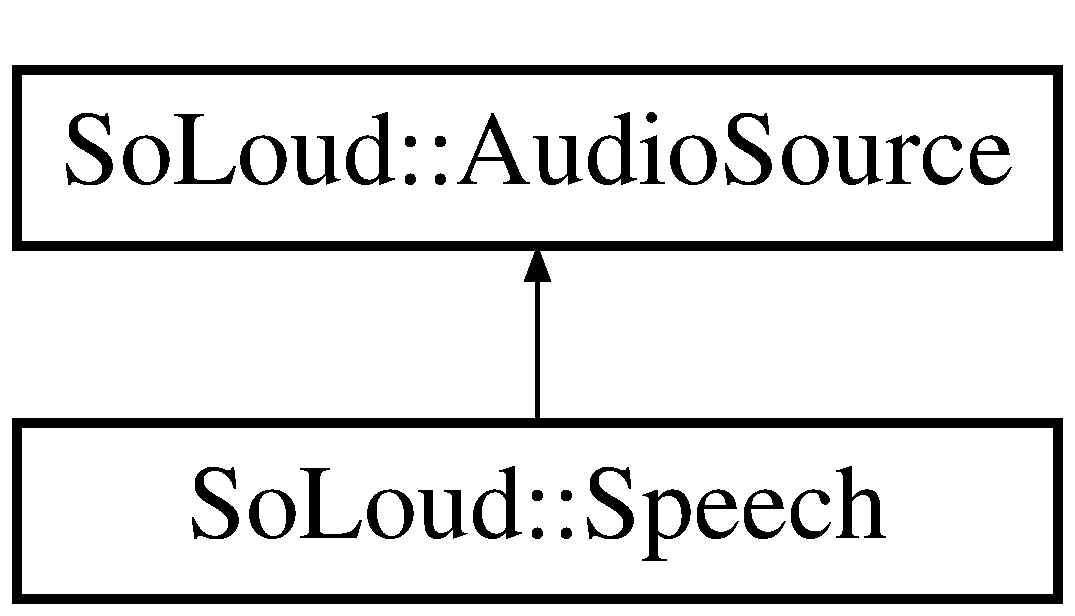
\includegraphics[height=2.000000cm]{class_so_loud_1_1_speech}
\end{center}
\end{figure}
\subsection*{Public Member Functions}
\begin{DoxyCompactItemize}
\item 
\mbox{\Hypertarget{class_so_loud_1_1_speech_a3c7ca61fa3aa9ce1d665b3fcc05dcfb4}\label{class_so_loud_1_1_speech_a3c7ca61fa3aa9ce1d665b3fcc05dcfb4}} 
result {\bfseries set\+Text} (const char $\ast$a\+Text)
\item 
\mbox{\Hypertarget{class_so_loud_1_1_speech_ad2a53fab95676c6e82f17a3535a81d6a}\label{class_so_loud_1_1_speech_ad2a53fab95676c6e82f17a3535a81d6a}} 
virtual \mbox{\hyperlink{class_so_loud_1_1_audio_source_instance}{Audio\+Source\+Instance}} $\ast$ {\bfseries create\+Instance} ()
\end{DoxyCompactItemize}
\subsection*{Public Attributes}
\begin{DoxyCompactItemize}
\item 
\mbox{\Hypertarget{class_so_loud_1_1_speech_ad62f0bffce5369f20004302215f3e80f}\label{class_so_loud_1_1_speech_ad62f0bffce5369f20004302215f3e80f}} 
int {\bfseries m\+Frames}
\item 
\mbox{\Hypertarget{class_so_loud_1_1_speech_a72021ae8bba4e2a66fa096de0bb0d0f8}\label{class_so_loud_1_1_speech_a72021ae8bba4e2a66fa096de0bb0d0f8}} 
darray {\bfseries m\+Element}
\end{DoxyCompactItemize}
\subsection*{Additional Inherited Members}


The documentation for this class was generated from the following file\+:\begin{DoxyCompactItemize}
\item 
deps/\+E\+S\+A\+T/include/\+E\+S\+A\+T\+\_\+extra/soloud/soloud\+\_\+speech.\+h\end{DoxyCompactItemize}

\hypertarget{class_so_loud_1_1_speech_instance}{}\section{So\+Loud\+:\+:Speech\+Instance Class Reference}
\label{class_so_loud_1_1_speech_instance}\index{So\+Loud\+::\+Speech\+Instance@{So\+Loud\+::\+Speech\+Instance}}
Inheritance diagram for So\+Loud\+:\+:Speech\+Instance\+:\begin{figure}[H]
\begin{center}
\leavevmode
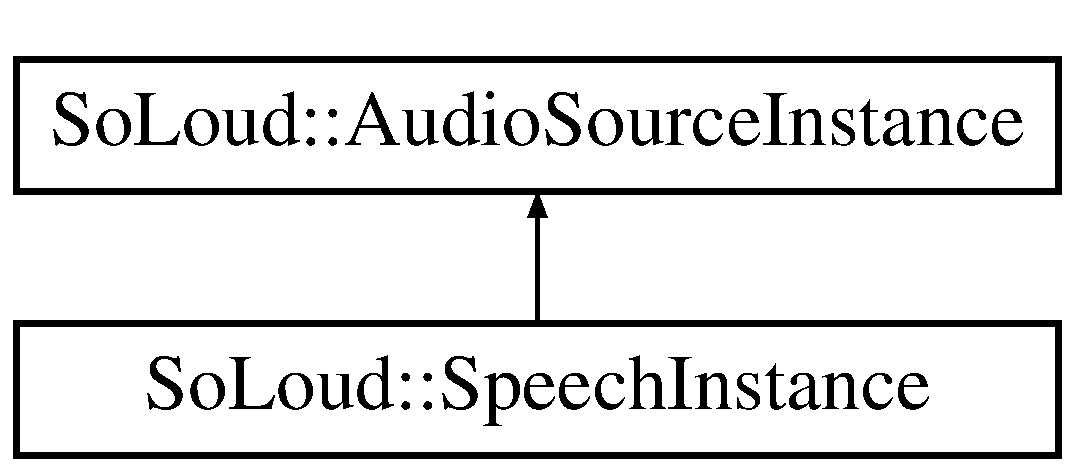
\includegraphics[height=2.000000cm]{class_so_loud_1_1_speech_instance}
\end{center}
\end{figure}
\subsection*{Public Member Functions}
\begin{DoxyCompactItemize}
\item 
\mbox{\Hypertarget{class_so_loud_1_1_speech_instance_a7fa645d0413fa76f3a7c6b4bd38e2602}\label{class_so_loud_1_1_speech_instance_a7fa645d0413fa76f3a7c6b4bd38e2602}} 
{\bfseries Speech\+Instance} (\mbox{\hyperlink{class_so_loud_1_1_speech}{Speech}} $\ast$a\+Parent)
\item 
\mbox{\Hypertarget{class_so_loud_1_1_speech_instance_aa279d6315a73f086279e5469f1e2e7dd}\label{class_so_loud_1_1_speech_instance_aa279d6315a73f086279e5469f1e2e7dd}} 
virtual void {\bfseries get\+Audio} (float $\ast$a\+Buffer, unsigned int a\+Samples)
\item 
\mbox{\Hypertarget{class_so_loud_1_1_speech_instance_a77294a31b9d70a07bc7ad3c0ecd8e843}\label{class_so_loud_1_1_speech_instance_a77294a31b9d70a07bc7ad3c0ecd8e843}} 
virtual result {\bfseries rewind} ()
\item 
\mbox{\Hypertarget{class_so_loud_1_1_speech_instance_a85f5788b39f0e1b7b68328706da81f1d}\label{class_so_loud_1_1_speech_instance_a85f5788b39f0e1b7b68328706da81f1d}} 
virtual bool {\bfseries has\+Ended} ()
\end{DoxyCompactItemize}
\subsection*{Additional Inherited Members}


The documentation for this class was generated from the following file\+:\begin{DoxyCompactItemize}
\item 
deps/\+E\+S\+A\+T/include/\+E\+S\+A\+T\+\_\+extra/soloud/soloud\+\_\+speech.\+h\end{DoxyCompactItemize}

\hypertarget{struct_e_s_a_t_1_1_sprite_transform}{}\section{E\+S\+AT\+:\+:Sprite\+Transform Struct Reference}
\label{struct_e_s_a_t_1_1_sprite_transform}\index{E\+S\+A\+T\+::\+Sprite\+Transform@{E\+S\+A\+T\+::\+Sprite\+Transform}}
\subsection*{Public Attributes}
\begin{DoxyCompactItemize}
\item 
\mbox{\Hypertarget{struct_e_s_a_t_1_1_sprite_transform_a6957a55ad5b47e8961d7efcd7f2a37de}\label{struct_e_s_a_t_1_1_sprite_transform_a6957a55ad5b47e8961d7efcd7f2a37de}} 
float {\bfseries x}
\item 
\mbox{\Hypertarget{struct_e_s_a_t_1_1_sprite_transform_acb0cdc468b660f7d274a533613196e0b}\label{struct_e_s_a_t_1_1_sprite_transform_acb0cdc468b660f7d274a533613196e0b}} 
float {\bfseries y}
\item 
\mbox{\Hypertarget{struct_e_s_a_t_1_1_sprite_transform_ae14e30796ad3662c7d90246cec556e62}\label{struct_e_s_a_t_1_1_sprite_transform_ae14e30796ad3662c7d90246cec556e62}} 
float {\bfseries angle}
\item 
\mbox{\Hypertarget{struct_e_s_a_t_1_1_sprite_transform_af5e4371f5bb605c2655ddb9df577ccf1}\label{struct_e_s_a_t_1_1_sprite_transform_af5e4371f5bb605c2655ddb9df577ccf1}} 
float {\bfseries scale\+\_\+x}
\item 
\mbox{\Hypertarget{struct_e_s_a_t_1_1_sprite_transform_aa76ca0269e377f60776089fd52d7fc44}\label{struct_e_s_a_t_1_1_sprite_transform_aa76ca0269e377f60776089fd52d7fc44}} 
float {\bfseries scale\+\_\+y}
\item 
\mbox{\Hypertarget{struct_e_s_a_t_1_1_sprite_transform_aeb05af8d0d355cb38d7948b82ed96ee3}\label{struct_e_s_a_t_1_1_sprite_transform_aeb05af8d0d355cb38d7948b82ed96ee3}} 
float {\bfseries sprite\+\_\+origin\+\_\+x}
\item 
\mbox{\Hypertarget{struct_e_s_a_t_1_1_sprite_transform_a0b09053286d716a3dc2c8b8379b81e79}\label{struct_e_s_a_t_1_1_sprite_transform_a0b09053286d716a3dc2c8b8379b81e79}} 
float {\bfseries sprite\+\_\+origin\+\_\+y}
\end{DoxyCompactItemize}


The documentation for this struct was generated from the following file\+:\begin{DoxyCompactItemize}
\item 
deps/\+E\+S\+A\+T/include/\+E\+S\+A\+T/sprite.\+h\end{DoxyCompactItemize}

\hypertarget{structsqlite3__api__routines}{}\section{sqlite3\+\_\+api\+\_\+routines Struct Reference}
\label{structsqlite3__api__routines}\index{sqlite3\+\_\+api\+\_\+routines@{sqlite3\+\_\+api\+\_\+routines}}
\subsection*{Public Attributes}
\begin{DoxyCompactItemize}
\item 
\mbox{\Hypertarget{structsqlite3__api__routines_a9ab2057c3042c5136b05f7daab66b4f4}\label{structsqlite3__api__routines_a9ab2057c3042c5136b05f7daab66b4f4}} 
void $\ast$($\ast$ {\bfseries aggregate\+\_\+context} )(sqlite3\+\_\+context $\ast$, int n\+Bytes)
\item 
\mbox{\Hypertarget{structsqlite3__api__routines_aa2f39986a5de8ec01fb5cb2aa573c08d}\label{structsqlite3__api__routines_aa2f39986a5de8ec01fb5cb2aa573c08d}} 
int($\ast$ {\bfseries aggregate\+\_\+count} )(sqlite3\+\_\+context $\ast$)
\item 
\mbox{\Hypertarget{structsqlite3__api__routines_a2e84de4afd1ba42151a75df4d7480a72}\label{structsqlite3__api__routines_a2e84de4afd1ba42151a75df4d7480a72}} 
int($\ast$ {\bfseries bind\+\_\+blob} )(sqlite3\+\_\+stmt $\ast$, int, const void $\ast$, int n, void($\ast$)(void $\ast$))
\item 
\mbox{\Hypertarget{structsqlite3__api__routines_abcdefbe78ab3ce4324d86651c03e8470}\label{structsqlite3__api__routines_abcdefbe78ab3ce4324d86651c03e8470}} 
int($\ast$ {\bfseries bind\+\_\+double} )(sqlite3\+\_\+stmt $\ast$, int, double)
\item 
\mbox{\Hypertarget{structsqlite3__api__routines_a70b6cc78957f11ff206df6125973daea}\label{structsqlite3__api__routines_a70b6cc78957f11ff206df6125973daea}} 
int($\ast$ {\bfseries bind\+\_\+int} )(sqlite3\+\_\+stmt $\ast$, int, int)
\item 
\mbox{\Hypertarget{structsqlite3__api__routines_ac71b110c165973291cc257973e7d6243}\label{structsqlite3__api__routines_ac71b110c165973291cc257973e7d6243}} 
int($\ast$ {\bfseries bind\+\_\+int64} )(sqlite3\+\_\+stmt $\ast$, int, sqlite\+\_\+int64)
\item 
\mbox{\Hypertarget{structsqlite3__api__routines_a78d546c352de656db3c15e7cc6255228}\label{structsqlite3__api__routines_a78d546c352de656db3c15e7cc6255228}} 
int($\ast$ {\bfseries bind\+\_\+null} )(sqlite3\+\_\+stmt $\ast$, int)
\item 
\mbox{\Hypertarget{structsqlite3__api__routines_acd345a944505eb7928568f01d7a4fe5a}\label{structsqlite3__api__routines_acd345a944505eb7928568f01d7a4fe5a}} 
int($\ast$ {\bfseries bind\+\_\+parameter\+\_\+count} )(sqlite3\+\_\+stmt $\ast$)
\item 
\mbox{\Hypertarget{structsqlite3__api__routines_af4ade5152fd51b1311463014b48dd05d}\label{structsqlite3__api__routines_af4ade5152fd51b1311463014b48dd05d}} 
int($\ast$ {\bfseries bind\+\_\+parameter\+\_\+index} )(sqlite3\+\_\+stmt $\ast$, const char $\ast$z\+Name)
\item 
\mbox{\Hypertarget{structsqlite3__api__routines_a9d8e99fd21fd5929fc6c254060d8f83b}\label{structsqlite3__api__routines_a9d8e99fd21fd5929fc6c254060d8f83b}} 
const char $\ast$($\ast$ {\bfseries bind\+\_\+parameter\+\_\+name} )(sqlite3\+\_\+stmt $\ast$, int)
\item 
\mbox{\Hypertarget{structsqlite3__api__routines_a0b489499ca3b7e212d25ea8a86d38f0e}\label{structsqlite3__api__routines_a0b489499ca3b7e212d25ea8a86d38f0e}} 
int($\ast$ {\bfseries bind\+\_\+text} )(sqlite3\+\_\+stmt $\ast$, int, const char $\ast$, int n, void($\ast$)(void $\ast$))
\item 
\mbox{\Hypertarget{structsqlite3__api__routines_ab6ad28704caf8337cf5a395154e8941c}\label{structsqlite3__api__routines_ab6ad28704caf8337cf5a395154e8941c}} 
int($\ast$ {\bfseries bind\+\_\+text16} )(sqlite3\+\_\+stmt $\ast$, int, const void $\ast$, int, void($\ast$)(void $\ast$))
\item 
\mbox{\Hypertarget{structsqlite3__api__routines_a8f3424b59d6bbc836c233a44a2fd9a36}\label{structsqlite3__api__routines_a8f3424b59d6bbc836c233a44a2fd9a36}} 
int($\ast$ {\bfseries bind\+\_\+value} )(sqlite3\+\_\+stmt $\ast$, int, const sqlite3\+\_\+value $\ast$)
\item 
\mbox{\Hypertarget{structsqlite3__api__routines_ad7b688e04d388cdeb13d4c06fedb1c46}\label{structsqlite3__api__routines_ad7b688e04d388cdeb13d4c06fedb1c46}} 
int($\ast$ {\bfseries busy\+\_\+handler} )(sqlite3 $\ast$, int($\ast$)(void $\ast$, int), void $\ast$)
\item 
\mbox{\Hypertarget{structsqlite3__api__routines_a8a4a2ccc0c7587e6c5c4db5f4b03246b}\label{structsqlite3__api__routines_a8a4a2ccc0c7587e6c5c4db5f4b03246b}} 
int($\ast$ {\bfseries busy\+\_\+timeout} )(sqlite3 $\ast$, int ms)
\item 
\mbox{\Hypertarget{structsqlite3__api__routines_aef4d7748f5708731e0aaf54dbfbbec33}\label{structsqlite3__api__routines_aef4d7748f5708731e0aaf54dbfbbec33}} 
int($\ast$ {\bfseries changes} )(sqlite3 $\ast$)
\item 
\mbox{\Hypertarget{structsqlite3__api__routines_a5c30292eef0130d7e8a408c4e3396012}\label{structsqlite3__api__routines_a5c30292eef0130d7e8a408c4e3396012}} 
int($\ast$ {\bfseries close} )(sqlite3 $\ast$)
\item 
\mbox{\Hypertarget{structsqlite3__api__routines_a4ecc8645b639cabe1fb630aceaec9017}\label{structsqlite3__api__routines_a4ecc8645b639cabe1fb630aceaec9017}} 
int($\ast$ {\bfseries collation\+\_\+needed} )(sqlite3 $\ast$, void $\ast$, void($\ast$)(void $\ast$, sqlite3 $\ast$, int e\+Text\+Rep, const char $\ast$))
\item 
\mbox{\Hypertarget{structsqlite3__api__routines_aa035538977ec61fe6df923b78db33962}\label{structsqlite3__api__routines_aa035538977ec61fe6df923b78db33962}} 
int($\ast$ {\bfseries collation\+\_\+needed16} )(sqlite3 $\ast$, void $\ast$, void($\ast$)(void $\ast$, sqlite3 $\ast$, int e\+Text\+Rep, const void $\ast$))
\item 
\mbox{\Hypertarget{structsqlite3__api__routines_aea28365a58adb937fbdf3983fe080e1a}\label{structsqlite3__api__routines_aea28365a58adb937fbdf3983fe080e1a}} 
const void $\ast$($\ast$ {\bfseries column\+\_\+blob} )(sqlite3\+\_\+stmt $\ast$, int i\+Col)
\item 
\mbox{\Hypertarget{structsqlite3__api__routines_a4925c38851818eebce76de641da69636}\label{structsqlite3__api__routines_a4925c38851818eebce76de641da69636}} 
int($\ast$ {\bfseries column\+\_\+bytes} )(sqlite3\+\_\+stmt $\ast$, int i\+Col)
\item 
\mbox{\Hypertarget{structsqlite3__api__routines_a7355fc82d2138b79b2e188fd2de4d269}\label{structsqlite3__api__routines_a7355fc82d2138b79b2e188fd2de4d269}} 
int($\ast$ {\bfseries column\+\_\+bytes16} )(sqlite3\+\_\+stmt $\ast$, int i\+Col)
\item 
\mbox{\Hypertarget{structsqlite3__api__routines_a3a41d82a8b13513a505889c8c9b1c97e}\label{structsqlite3__api__routines_a3a41d82a8b13513a505889c8c9b1c97e}} 
int($\ast$ {\bfseries column\+\_\+count} )(sqlite3\+\_\+stmt $\ast$p\+Stmt)
\item 
\mbox{\Hypertarget{structsqlite3__api__routines_acd92d7b8700122a8c352d9f03c8fad37}\label{structsqlite3__api__routines_acd92d7b8700122a8c352d9f03c8fad37}} 
const char $\ast$($\ast$ {\bfseries column\+\_\+database\+\_\+name} )(sqlite3\+\_\+stmt $\ast$, int)
\item 
\mbox{\Hypertarget{structsqlite3__api__routines_a3e38edb955dbd932717bb11283b65490}\label{structsqlite3__api__routines_a3e38edb955dbd932717bb11283b65490}} 
const void $\ast$($\ast$ {\bfseries column\+\_\+database\+\_\+name16} )(sqlite3\+\_\+stmt $\ast$, int)
\item 
\mbox{\Hypertarget{structsqlite3__api__routines_ae4e78358b212d7d37aa3a47058614c6f}\label{structsqlite3__api__routines_ae4e78358b212d7d37aa3a47058614c6f}} 
const char $\ast$($\ast$ {\bfseries column\+\_\+decltype} )(sqlite3\+\_\+stmt $\ast$, int i)
\item 
\mbox{\Hypertarget{structsqlite3__api__routines_af5504d756c0ad0526acd0c44f9b2239a}\label{structsqlite3__api__routines_af5504d756c0ad0526acd0c44f9b2239a}} 
const void $\ast$($\ast$ {\bfseries column\+\_\+decltype16} )(sqlite3\+\_\+stmt $\ast$, int)
\item 
\mbox{\Hypertarget{structsqlite3__api__routines_a6f10fb7f35cebf6cb62a77adfdc70efc}\label{structsqlite3__api__routines_a6f10fb7f35cebf6cb62a77adfdc70efc}} 
double($\ast$ {\bfseries column\+\_\+double} )(sqlite3\+\_\+stmt $\ast$, int i\+Col)
\item 
\mbox{\Hypertarget{structsqlite3__api__routines_a066b63e4ca0f83af9eaba45b8db3e6be}\label{structsqlite3__api__routines_a066b63e4ca0f83af9eaba45b8db3e6be}} 
int($\ast$ {\bfseries column\+\_\+int} )(sqlite3\+\_\+stmt $\ast$, int i\+Col)
\item 
\mbox{\Hypertarget{structsqlite3__api__routines_a6992d17196cce6a9c893df0e69ea8b17}\label{structsqlite3__api__routines_a6992d17196cce6a9c893df0e69ea8b17}} 
sqlite\+\_\+int64($\ast$ {\bfseries column\+\_\+int64} )(sqlite3\+\_\+stmt $\ast$, int i\+Col)
\item 
\mbox{\Hypertarget{structsqlite3__api__routines_a8ae08c78d80fae61c0abeb80a7cd70f5}\label{structsqlite3__api__routines_a8ae08c78d80fae61c0abeb80a7cd70f5}} 
const char $\ast$($\ast$ {\bfseries column\+\_\+name} )(sqlite3\+\_\+stmt $\ast$, int)
\item 
\mbox{\Hypertarget{structsqlite3__api__routines_a14ff9b029639553e11e610281097dfc7}\label{structsqlite3__api__routines_a14ff9b029639553e11e610281097dfc7}} 
const void $\ast$($\ast$ {\bfseries column\+\_\+name16} )(sqlite3\+\_\+stmt $\ast$, int)
\item 
\mbox{\Hypertarget{structsqlite3__api__routines_a944609a2b514a9002e3c76575ad3bd65}\label{structsqlite3__api__routines_a944609a2b514a9002e3c76575ad3bd65}} 
const char $\ast$($\ast$ {\bfseries column\+\_\+origin\+\_\+name} )(sqlite3\+\_\+stmt $\ast$, int)
\item 
\mbox{\Hypertarget{structsqlite3__api__routines_a29f148c32e2e8aba50d3ff3ffd8c4f90}\label{structsqlite3__api__routines_a29f148c32e2e8aba50d3ff3ffd8c4f90}} 
const void $\ast$($\ast$ {\bfseries column\+\_\+origin\+\_\+name16} )(sqlite3\+\_\+stmt $\ast$, int)
\item 
\mbox{\Hypertarget{structsqlite3__api__routines_a06525d1223f774274ff49b287d33a952}\label{structsqlite3__api__routines_a06525d1223f774274ff49b287d33a952}} 
const char $\ast$($\ast$ {\bfseries column\+\_\+table\+\_\+name} )(sqlite3\+\_\+stmt $\ast$, int)
\item 
\mbox{\Hypertarget{structsqlite3__api__routines_a3252c82d0f2ed7e88a76f26585d13bbb}\label{structsqlite3__api__routines_a3252c82d0f2ed7e88a76f26585d13bbb}} 
const void $\ast$($\ast$ {\bfseries column\+\_\+table\+\_\+name16} )(sqlite3\+\_\+stmt $\ast$, int)
\item 
\mbox{\Hypertarget{structsqlite3__api__routines_ae9bb95b6e37236693ca5ec51598c7908}\label{structsqlite3__api__routines_ae9bb95b6e37236693ca5ec51598c7908}} 
const unsigned char $\ast$($\ast$ {\bfseries column\+\_\+text} )(sqlite3\+\_\+stmt $\ast$, int i\+Col)
\item 
\mbox{\Hypertarget{structsqlite3__api__routines_a952f4680bde7ff3af3ada148380ec08e}\label{structsqlite3__api__routines_a952f4680bde7ff3af3ada148380ec08e}} 
const void $\ast$($\ast$ {\bfseries column\+\_\+text16} )(sqlite3\+\_\+stmt $\ast$, int i\+Col)
\item 
\mbox{\Hypertarget{structsqlite3__api__routines_a1381e48828398ae738aa2416d2e4feb9}\label{structsqlite3__api__routines_a1381e48828398ae738aa2416d2e4feb9}} 
int($\ast$ {\bfseries column\+\_\+type} )(sqlite3\+\_\+stmt $\ast$, int i\+Col)
\item 
\mbox{\Hypertarget{structsqlite3__api__routines_a1ca935310e3637179f857791ccb42116}\label{structsqlite3__api__routines_a1ca935310e3637179f857791ccb42116}} 
sqlite3\+\_\+value $\ast$($\ast$ {\bfseries column\+\_\+value} )(sqlite3\+\_\+stmt $\ast$, int i\+Col)
\item 
\mbox{\Hypertarget{structsqlite3__api__routines_a906bf080c41a7b3379866e08fe9f3db8}\label{structsqlite3__api__routines_a906bf080c41a7b3379866e08fe9f3db8}} 
void $\ast$($\ast$ {\bfseries commit\+\_\+hook} )(sqlite3 $\ast$, int($\ast$)(void $\ast$), void $\ast$)
\item 
\mbox{\Hypertarget{structsqlite3__api__routines_acf6be6ede31fda32f4f0193aafce0ba3}\label{structsqlite3__api__routines_acf6be6ede31fda32f4f0193aafce0ba3}} 
int($\ast$ {\bfseries complete} )(const char $\ast$sql)
\item 
\mbox{\Hypertarget{structsqlite3__api__routines_a12b69b88bc84fba6fe97cefa4b979eff}\label{structsqlite3__api__routines_a12b69b88bc84fba6fe97cefa4b979eff}} 
int($\ast$ {\bfseries complete16} )(const void $\ast$sql)
\item 
\mbox{\Hypertarget{structsqlite3__api__routines_a923433105b84b919ea359ef320da55b1}\label{structsqlite3__api__routines_a923433105b84b919ea359ef320da55b1}} 
int($\ast$ {\bfseries create\+\_\+collation} )(sqlite3 $\ast$, const char $\ast$, int, void $\ast$, int($\ast$)(void $\ast$, int, const void $\ast$, int, const void $\ast$))
\item 
\mbox{\Hypertarget{structsqlite3__api__routines_ab3fe60d5c018e3ffcad08bec34dc53e7}\label{structsqlite3__api__routines_ab3fe60d5c018e3ffcad08bec34dc53e7}} 
int($\ast$ {\bfseries create\+\_\+collation16} )(sqlite3 $\ast$, const void $\ast$, int, void $\ast$, int($\ast$)(void $\ast$, int, const void $\ast$, int, const void $\ast$))
\item 
\mbox{\Hypertarget{structsqlite3__api__routines_a9f15bf465292b7176eddbf0287c770f8}\label{structsqlite3__api__routines_a9f15bf465292b7176eddbf0287c770f8}} 
int($\ast$ {\bfseries create\+\_\+function} )(sqlite3 $\ast$, const char $\ast$, int, int, void $\ast$, void($\ast$x\+Func)(sqlite3\+\_\+context $\ast$, int, sqlite3\+\_\+value $\ast$$\ast$), void($\ast$x\+Step)(sqlite3\+\_\+context $\ast$, int, sqlite3\+\_\+value $\ast$$\ast$), void($\ast$x\+Final)(sqlite3\+\_\+context $\ast$))
\item 
\mbox{\Hypertarget{structsqlite3__api__routines_a2cb97ce7512759a08f1744e24cd0294f}\label{structsqlite3__api__routines_a2cb97ce7512759a08f1744e24cd0294f}} 
int($\ast$ {\bfseries create\+\_\+function16} )(sqlite3 $\ast$, const void $\ast$, int, int, void $\ast$, void($\ast$x\+Func)(sqlite3\+\_\+context $\ast$, int, sqlite3\+\_\+value $\ast$$\ast$), void($\ast$x\+Step)(sqlite3\+\_\+context $\ast$, int, sqlite3\+\_\+value $\ast$$\ast$), void($\ast$x\+Final)(sqlite3\+\_\+context $\ast$))
\item 
\mbox{\Hypertarget{structsqlite3__api__routines_a0d2bee02b4c2ce95aa3ae6d4b904bff6}\label{structsqlite3__api__routines_a0d2bee02b4c2ce95aa3ae6d4b904bff6}} 
int($\ast$ {\bfseries create\+\_\+module} )(sqlite3 $\ast$, const char $\ast$, const \mbox{\hyperlink{structsqlite3__module}{sqlite3\+\_\+module}} $\ast$, void $\ast$)
\item 
\mbox{\Hypertarget{structsqlite3__api__routines_a4d248c8b990dc7b96c5734ec878508a0}\label{structsqlite3__api__routines_a4d248c8b990dc7b96c5734ec878508a0}} 
int($\ast$ {\bfseries data\+\_\+count} )(sqlite3\+\_\+stmt $\ast$p\+Stmt)
\item 
\mbox{\Hypertarget{structsqlite3__api__routines_a202912ed0777c34ef98ab262204d0c6e}\label{structsqlite3__api__routines_a202912ed0777c34ef98ab262204d0c6e}} 
sqlite3 $\ast$($\ast$ {\bfseries db\+\_\+handle} )(sqlite3\+\_\+stmt $\ast$)
\item 
\mbox{\Hypertarget{structsqlite3__api__routines_abe47369f89df1193ca28751e8d024818}\label{structsqlite3__api__routines_abe47369f89df1193ca28751e8d024818}} 
int($\ast$ {\bfseries declare\+\_\+vtab} )(sqlite3 $\ast$, const char $\ast$)
\item 
\mbox{\Hypertarget{structsqlite3__api__routines_ae67da9e0a3629fd1fd46fd73389d8c98}\label{structsqlite3__api__routines_ae67da9e0a3629fd1fd46fd73389d8c98}} 
int($\ast$ {\bfseries enable\+\_\+shared\+\_\+cache} )(int)
\item 
\mbox{\Hypertarget{structsqlite3__api__routines_a1a985d959eafe6f293e41a5ca1d1a2e9}\label{structsqlite3__api__routines_a1a985d959eafe6f293e41a5ca1d1a2e9}} 
int($\ast$ {\bfseries errcode} )(sqlite3 $\ast$db)
\item 
\mbox{\Hypertarget{structsqlite3__api__routines_a69002673143895d276850a400e7955d7}\label{structsqlite3__api__routines_a69002673143895d276850a400e7955d7}} 
const char $\ast$($\ast$ {\bfseries errmsg} )(sqlite3 $\ast$)
\item 
\mbox{\Hypertarget{structsqlite3__api__routines_a1392e153c69f5b32fd8acc19cb780baf}\label{structsqlite3__api__routines_a1392e153c69f5b32fd8acc19cb780baf}} 
const void $\ast$($\ast$ {\bfseries errmsg16} )(sqlite3 $\ast$)
\item 
\mbox{\Hypertarget{structsqlite3__api__routines_ac6476ec4fd66eb629942bd60a47adf76}\label{structsqlite3__api__routines_ac6476ec4fd66eb629942bd60a47adf76}} 
int($\ast$ {\bfseries exec} )(sqlite3 $\ast$, const char $\ast$, sqlite3\+\_\+callback, void $\ast$, char $\ast$$\ast$)
\item 
\mbox{\Hypertarget{structsqlite3__api__routines_aaf5ef34c7b325eefb8459224a5c926e8}\label{structsqlite3__api__routines_aaf5ef34c7b325eefb8459224a5c926e8}} 
int($\ast$ {\bfseries expired} )(sqlite3\+\_\+stmt $\ast$)
\item 
\mbox{\Hypertarget{structsqlite3__api__routines_a0bbe0b1cdd61a2e7e089ad1e42978f6f}\label{structsqlite3__api__routines_a0bbe0b1cdd61a2e7e089ad1e42978f6f}} 
int($\ast$ {\bfseries finalize} )(sqlite3\+\_\+stmt $\ast$p\+Stmt)
\item 
\mbox{\Hypertarget{structsqlite3__api__routines_a7418560cd2dacb9a6cb0b7f5e3082787}\label{structsqlite3__api__routines_a7418560cd2dacb9a6cb0b7f5e3082787}} 
void($\ast$ {\bfseries free} )(void $\ast$)
\item 
\mbox{\Hypertarget{structsqlite3__api__routines_aa94faa431905ee9d04bb93cbce735a0c}\label{structsqlite3__api__routines_aa94faa431905ee9d04bb93cbce735a0c}} 
void($\ast$ {\bfseries free\+\_\+table} )(char $\ast$$\ast$result)
\item 
\mbox{\Hypertarget{structsqlite3__api__routines_ae37e25adf7b17f97387fa1ac36094988}\label{structsqlite3__api__routines_ae37e25adf7b17f97387fa1ac36094988}} 
int($\ast$ {\bfseries get\+\_\+autocommit} )(sqlite3 $\ast$)
\item 
\mbox{\Hypertarget{structsqlite3__api__routines_a1be39621e5074afbd0a81f105105866e}\label{structsqlite3__api__routines_a1be39621e5074afbd0a81f105105866e}} 
void $\ast$($\ast$ {\bfseries get\+\_\+auxdata} )(sqlite3\+\_\+context $\ast$, int)
\item 
\mbox{\Hypertarget{structsqlite3__api__routines_a3a265a9fa59237ed1630acf4b4f5efc4}\label{structsqlite3__api__routines_a3a265a9fa59237ed1630acf4b4f5efc4}} 
int($\ast$ {\bfseries get\+\_\+table} )(sqlite3 $\ast$, const char $\ast$, char $\ast$$\ast$$\ast$, int $\ast$, int $\ast$, char $\ast$$\ast$)
\item 
\mbox{\Hypertarget{structsqlite3__api__routines_a11d469bd09340c52991a7d87fe212395}\label{structsqlite3__api__routines_a11d469bd09340c52991a7d87fe212395}} 
int($\ast$ {\bfseries global\+\_\+recover} )(void)
\item 
\mbox{\Hypertarget{structsqlite3__api__routines_adab3cdd36976fa72f7e6662f597818ea}\label{structsqlite3__api__routines_adab3cdd36976fa72f7e6662f597818ea}} 
void($\ast$ {\bfseries interruptx} )(sqlite3 $\ast$)
\item 
\mbox{\Hypertarget{structsqlite3__api__routines_a6e69f8e7d32673cf778b58d0856e6dc7}\label{structsqlite3__api__routines_a6e69f8e7d32673cf778b58d0856e6dc7}} 
sqlite\+\_\+int64($\ast$ {\bfseries last\+\_\+insert\+\_\+rowid} )(sqlite3 $\ast$)
\item 
\mbox{\Hypertarget{structsqlite3__api__routines_ac60b467b55897230bf12dc593ca561e8}\label{structsqlite3__api__routines_ac60b467b55897230bf12dc593ca561e8}} 
const char $\ast$($\ast$ {\bfseries libversion} )(void)
\item 
\mbox{\Hypertarget{structsqlite3__api__routines_ad33f785fe5f26b534a570c9055a34858}\label{structsqlite3__api__routines_ad33f785fe5f26b534a570c9055a34858}} 
int($\ast$ {\bfseries libversion\+\_\+number} )(void)
\item 
\mbox{\Hypertarget{structsqlite3__api__routines_a1c4b2c2102460266ffb4e7609708684a}\label{structsqlite3__api__routines_a1c4b2c2102460266ffb4e7609708684a}} 
void $\ast$($\ast$ {\bfseries malloc} )(int)
\item 
\mbox{\Hypertarget{structsqlite3__api__routines_ac9a1fb416ae25745652d363a833ee977}\label{structsqlite3__api__routines_ac9a1fb416ae25745652d363a833ee977}} 
char $\ast$($\ast$ {\bfseries mprintf} )(const char $\ast$,...)
\item 
\mbox{\Hypertarget{structsqlite3__api__routines_acc0adb13d6e87651add47577dd57e997}\label{structsqlite3__api__routines_acc0adb13d6e87651add47577dd57e997}} 
int($\ast$ {\bfseries open} )(const char $\ast$, sqlite3 $\ast$$\ast$)
\item 
\mbox{\Hypertarget{structsqlite3__api__routines_a58d3ff1185d4aae08c6be2b71c4a2e23}\label{structsqlite3__api__routines_a58d3ff1185d4aae08c6be2b71c4a2e23}} 
int($\ast$ {\bfseries open16} )(const void $\ast$, sqlite3 $\ast$$\ast$)
\item 
\mbox{\Hypertarget{structsqlite3__api__routines_a506ea7218da25d4973721f4770ce8dc7}\label{structsqlite3__api__routines_a506ea7218da25d4973721f4770ce8dc7}} 
int($\ast$ {\bfseries prepare} )(sqlite3 $\ast$, const char $\ast$, int, sqlite3\+\_\+stmt $\ast$$\ast$, const char $\ast$$\ast$)
\item 
\mbox{\Hypertarget{structsqlite3__api__routines_a6f08b1665a9ac05e3b7fab0bd8adce32}\label{structsqlite3__api__routines_a6f08b1665a9ac05e3b7fab0bd8adce32}} 
int($\ast$ {\bfseries prepare16} )(sqlite3 $\ast$, const void $\ast$, int, sqlite3\+\_\+stmt $\ast$$\ast$, const void $\ast$$\ast$)
\item 
\mbox{\Hypertarget{structsqlite3__api__routines_afa3554d38034ec4c0a339e2e908732db}\label{structsqlite3__api__routines_afa3554d38034ec4c0a339e2e908732db}} 
void $\ast$($\ast$ {\bfseries profile} )(sqlite3 $\ast$, void($\ast$)(void $\ast$, const char $\ast$, sqlite\+\_\+uint64), void $\ast$)
\item 
\mbox{\Hypertarget{structsqlite3__api__routines_a58d79a7091ade0d1630d62ecf1931e9d}\label{structsqlite3__api__routines_a58d79a7091ade0d1630d62ecf1931e9d}} 
void($\ast$ {\bfseries progress\+\_\+handler} )(sqlite3 $\ast$, int, int($\ast$)(void $\ast$), void $\ast$)
\item 
\mbox{\Hypertarget{structsqlite3__api__routines_a40270284cc1abb0818ade7b41351bb5b}\label{structsqlite3__api__routines_a40270284cc1abb0818ade7b41351bb5b}} 
void $\ast$($\ast$ {\bfseries realloc} )(void $\ast$, int)
\item 
\mbox{\Hypertarget{structsqlite3__api__routines_a88551d8943b8f9cdc7abebac90998ddf}\label{structsqlite3__api__routines_a88551d8943b8f9cdc7abebac90998ddf}} 
int($\ast$ {\bfseries reset} )(sqlite3\+\_\+stmt $\ast$p\+Stmt)
\item 
\mbox{\Hypertarget{structsqlite3__api__routines_a7151cedc160519771de48f9dab665356}\label{structsqlite3__api__routines_a7151cedc160519771de48f9dab665356}} 
void($\ast$ {\bfseries result\+\_\+blob} )(sqlite3\+\_\+context $\ast$, const void $\ast$, int, void($\ast$)(void $\ast$))
\item 
\mbox{\Hypertarget{structsqlite3__api__routines_ae5babdc991a56b484bc7a66a993435f3}\label{structsqlite3__api__routines_ae5babdc991a56b484bc7a66a993435f3}} 
void($\ast$ {\bfseries result\+\_\+double} )(sqlite3\+\_\+context $\ast$, double)
\item 
\mbox{\Hypertarget{structsqlite3__api__routines_ac80d799ae1e99289af007d9690ae3085}\label{structsqlite3__api__routines_ac80d799ae1e99289af007d9690ae3085}} 
void($\ast$ {\bfseries result\+\_\+error} )(sqlite3\+\_\+context $\ast$, const char $\ast$, int)
\item 
\mbox{\Hypertarget{structsqlite3__api__routines_aa5c6ea660625078a1256a548d8e746ba}\label{structsqlite3__api__routines_aa5c6ea660625078a1256a548d8e746ba}} 
void($\ast$ {\bfseries result\+\_\+error16} )(sqlite3\+\_\+context $\ast$, const void $\ast$, int)
\item 
\mbox{\Hypertarget{structsqlite3__api__routines_ad1470bb8057593e97170b73b65a9e808}\label{structsqlite3__api__routines_ad1470bb8057593e97170b73b65a9e808}} 
void($\ast$ {\bfseries result\+\_\+int} )(sqlite3\+\_\+context $\ast$, int)
\item 
\mbox{\Hypertarget{structsqlite3__api__routines_ae24ce0ec8d90ac28a6a98cfafadaa7d0}\label{structsqlite3__api__routines_ae24ce0ec8d90ac28a6a98cfafadaa7d0}} 
void($\ast$ {\bfseries result\+\_\+int64} )(sqlite3\+\_\+context $\ast$, sqlite\+\_\+int64)
\item 
\mbox{\Hypertarget{structsqlite3__api__routines_ab7552d3c8d27f332cb34c45ce9f7b290}\label{structsqlite3__api__routines_ab7552d3c8d27f332cb34c45ce9f7b290}} 
void($\ast$ {\bfseries result\+\_\+null} )(sqlite3\+\_\+context $\ast$)
\item 
\mbox{\Hypertarget{structsqlite3__api__routines_abf4e25b69248ca865953d0d0768aa8c0}\label{structsqlite3__api__routines_abf4e25b69248ca865953d0d0768aa8c0}} 
void($\ast$ {\bfseries result\+\_\+text} )(sqlite3\+\_\+context $\ast$, const char $\ast$, int, void($\ast$)(void $\ast$))
\item 
\mbox{\Hypertarget{structsqlite3__api__routines_ac7d4e41cae34faec587e871f91a0691d}\label{structsqlite3__api__routines_ac7d4e41cae34faec587e871f91a0691d}} 
void($\ast$ {\bfseries result\+\_\+text16} )(sqlite3\+\_\+context $\ast$, const void $\ast$, int, void($\ast$)(void $\ast$))
\item 
\mbox{\Hypertarget{structsqlite3__api__routines_a953fc695bbec79fc5999bc9f2a0c94f3}\label{structsqlite3__api__routines_a953fc695bbec79fc5999bc9f2a0c94f3}} 
void($\ast$ {\bfseries result\+\_\+text16be} )(sqlite3\+\_\+context $\ast$, const void $\ast$, int, void($\ast$)(void $\ast$))
\item 
\mbox{\Hypertarget{structsqlite3__api__routines_a6607ea8847a57d49bdf450205f4d580f}\label{structsqlite3__api__routines_a6607ea8847a57d49bdf450205f4d580f}} 
void($\ast$ {\bfseries result\+\_\+text16le} )(sqlite3\+\_\+context $\ast$, const void $\ast$, int, void($\ast$)(void $\ast$))
\item 
\mbox{\Hypertarget{structsqlite3__api__routines_a077437fd729730e66afab9eb487ca10c}\label{structsqlite3__api__routines_a077437fd729730e66afab9eb487ca10c}} 
void($\ast$ {\bfseries result\+\_\+value} )(sqlite3\+\_\+context $\ast$, sqlite3\+\_\+value $\ast$)
\item 
\mbox{\Hypertarget{structsqlite3__api__routines_ac0784da0f9e7abd1cd8417a37e593aaf}\label{structsqlite3__api__routines_ac0784da0f9e7abd1cd8417a37e593aaf}} 
void $\ast$($\ast$ {\bfseries rollback\+\_\+hook} )(sqlite3 $\ast$, void($\ast$)(void $\ast$), void $\ast$)
\item 
\mbox{\Hypertarget{structsqlite3__api__routines_a6d9843596d2d01e52eec89ab50ca6f27}\label{structsqlite3__api__routines_a6d9843596d2d01e52eec89ab50ca6f27}} 
int($\ast$ {\bfseries set\+\_\+authorizer} )(sqlite3 $\ast$, int($\ast$)(void $\ast$, int, const char $\ast$, const char $\ast$, const char $\ast$, const char $\ast$), void $\ast$)
\item 
\mbox{\Hypertarget{structsqlite3__api__routines_a9e2419b4ef954a24408d3c12fe2b1dd7}\label{structsqlite3__api__routines_a9e2419b4ef954a24408d3c12fe2b1dd7}} 
void($\ast$ {\bfseries set\+\_\+auxdata} )(sqlite3\+\_\+context $\ast$, int, void $\ast$, void($\ast$)(void $\ast$))
\item 
\mbox{\Hypertarget{structsqlite3__api__routines_ad038a8026d6c9026284fe6a15fef7a72}\label{structsqlite3__api__routines_ad038a8026d6c9026284fe6a15fef7a72}} 
char $\ast$($\ast$ {\bfseries snprintf} )(int, char $\ast$, const char $\ast$,...)
\item 
\mbox{\Hypertarget{structsqlite3__api__routines_ad83c0c75185e68a850ec912cb886af0d}\label{structsqlite3__api__routines_ad83c0c75185e68a850ec912cb886af0d}} 
int($\ast$ {\bfseries step} )(sqlite3\+\_\+stmt $\ast$)
\item 
\mbox{\Hypertarget{structsqlite3__api__routines_a8f0cef68458ef530829177f7ca5168f9}\label{structsqlite3__api__routines_a8f0cef68458ef530829177f7ca5168f9}} 
int($\ast$ {\bfseries table\+\_\+column\+\_\+metadata} )(sqlite3 $\ast$, const char $\ast$, const char $\ast$, const char $\ast$, char const $\ast$$\ast$, char const $\ast$$\ast$, int $\ast$, int $\ast$, int $\ast$)
\item 
\mbox{\Hypertarget{structsqlite3__api__routines_a9225dd1e2e76c3ce649c68e2a0b0f5f5}\label{structsqlite3__api__routines_a9225dd1e2e76c3ce649c68e2a0b0f5f5}} 
void($\ast$ {\bfseries thread\+\_\+cleanup} )(void)
\item 
\mbox{\Hypertarget{structsqlite3__api__routines_a354c6e15df905db1db95bfc348ce98a8}\label{structsqlite3__api__routines_a354c6e15df905db1db95bfc348ce98a8}} 
int($\ast$ {\bfseries total\+\_\+changes} )(sqlite3 $\ast$)
\item 
\mbox{\Hypertarget{structsqlite3__api__routines_ad747f6107d6a8edaefebc52cce2679d3}\label{structsqlite3__api__routines_ad747f6107d6a8edaefebc52cce2679d3}} 
void $\ast$($\ast$ {\bfseries trace} )(sqlite3 $\ast$, void($\ast$x\+Trace)(void $\ast$, const char $\ast$), void $\ast$)
\item 
\mbox{\Hypertarget{structsqlite3__api__routines_ab3c5b0d61682151cd3c8419eb4c1ca13}\label{structsqlite3__api__routines_ab3c5b0d61682151cd3c8419eb4c1ca13}} 
int($\ast$ {\bfseries transfer\+\_\+bindings} )(sqlite3\+\_\+stmt $\ast$, sqlite3\+\_\+stmt $\ast$)
\item 
\mbox{\Hypertarget{structsqlite3__api__routines_a85cffd9c5f77524f9b74292994b4b205}\label{structsqlite3__api__routines_a85cffd9c5f77524f9b74292994b4b205}} 
void $\ast$($\ast$ {\bfseries update\+\_\+hook} )(sqlite3 $\ast$, void($\ast$)(void $\ast$, int, char const $\ast$, char const $\ast$, sqlite\+\_\+int64), void $\ast$)
\item 
\mbox{\Hypertarget{structsqlite3__api__routines_a4e066cc9b45c788202731ab113711833}\label{structsqlite3__api__routines_a4e066cc9b45c788202731ab113711833}} 
void $\ast$($\ast$ {\bfseries user\+\_\+data} )(sqlite3\+\_\+context $\ast$)
\item 
\mbox{\Hypertarget{structsqlite3__api__routines_ae2c90149043ca50502c7d6b7e1764103}\label{structsqlite3__api__routines_ae2c90149043ca50502c7d6b7e1764103}} 
const void $\ast$($\ast$ {\bfseries value\+\_\+blob} )(sqlite3\+\_\+value $\ast$)
\item 
\mbox{\Hypertarget{structsqlite3__api__routines_aaf6e53b347fe8a81b05f8144c1418022}\label{structsqlite3__api__routines_aaf6e53b347fe8a81b05f8144c1418022}} 
int($\ast$ {\bfseries value\+\_\+bytes} )(sqlite3\+\_\+value $\ast$)
\item 
\mbox{\Hypertarget{structsqlite3__api__routines_ad1e6349c107a4e9640d0f70a1032d9c9}\label{structsqlite3__api__routines_ad1e6349c107a4e9640d0f70a1032d9c9}} 
int($\ast$ {\bfseries value\+\_\+bytes16} )(sqlite3\+\_\+value $\ast$)
\item 
\mbox{\Hypertarget{structsqlite3__api__routines_a038780bf33da5a73ade808c2fbeb7f91}\label{structsqlite3__api__routines_a038780bf33da5a73ade808c2fbeb7f91}} 
double($\ast$ {\bfseries value\+\_\+double} )(sqlite3\+\_\+value $\ast$)
\item 
\mbox{\Hypertarget{structsqlite3__api__routines_aaea71f352f2637f7d43781cd279ece62}\label{structsqlite3__api__routines_aaea71f352f2637f7d43781cd279ece62}} 
int($\ast$ {\bfseries value\+\_\+int} )(sqlite3\+\_\+value $\ast$)
\item 
\mbox{\Hypertarget{structsqlite3__api__routines_a27cfd29e44574a9b10f0a7cb3a7c9ada}\label{structsqlite3__api__routines_a27cfd29e44574a9b10f0a7cb3a7c9ada}} 
sqlite\+\_\+int64($\ast$ {\bfseries value\+\_\+int64} )(sqlite3\+\_\+value $\ast$)
\item 
\mbox{\Hypertarget{structsqlite3__api__routines_a870e384ce2056e1e608808f8527af223}\label{structsqlite3__api__routines_a870e384ce2056e1e608808f8527af223}} 
int($\ast$ {\bfseries value\+\_\+numeric\+\_\+type} )(sqlite3\+\_\+value $\ast$)
\item 
\mbox{\Hypertarget{structsqlite3__api__routines_ae83b9c4efba57334d83c50f59569a161}\label{structsqlite3__api__routines_ae83b9c4efba57334d83c50f59569a161}} 
const unsigned char $\ast$($\ast$ {\bfseries value\+\_\+text} )(sqlite3\+\_\+value $\ast$)
\item 
\mbox{\Hypertarget{structsqlite3__api__routines_ab58872245de9133b18ea75f2895bf0d9}\label{structsqlite3__api__routines_ab58872245de9133b18ea75f2895bf0d9}} 
const void $\ast$($\ast$ {\bfseries value\+\_\+text16} )(sqlite3\+\_\+value $\ast$)
\item 
\mbox{\Hypertarget{structsqlite3__api__routines_af21386f3f28a2deefa8fe73d07c6f7ca}\label{structsqlite3__api__routines_af21386f3f28a2deefa8fe73d07c6f7ca}} 
const void $\ast$($\ast$ {\bfseries value\+\_\+text16be} )(sqlite3\+\_\+value $\ast$)
\item 
\mbox{\Hypertarget{structsqlite3__api__routines_a1a99f053ce6183ec8fcb007e7b66a43c}\label{structsqlite3__api__routines_a1a99f053ce6183ec8fcb007e7b66a43c}} 
const void $\ast$($\ast$ {\bfseries value\+\_\+text16le} )(sqlite3\+\_\+value $\ast$)
\item 
\mbox{\Hypertarget{structsqlite3__api__routines_a30e5d5464fae02a66e73c0ee6afa3a0d}\label{structsqlite3__api__routines_a30e5d5464fae02a66e73c0ee6afa3a0d}} 
int($\ast$ {\bfseries value\+\_\+type} )(sqlite3\+\_\+value $\ast$)
\item 
\mbox{\Hypertarget{structsqlite3__api__routines_a64e9921dc2f462a9307dfcfde54ba849}\label{structsqlite3__api__routines_a64e9921dc2f462a9307dfcfde54ba849}} 
char $\ast$($\ast$ {\bfseries vmprintf} )(const char $\ast$, va\+\_\+list)
\item 
\mbox{\Hypertarget{structsqlite3__api__routines_a44b969d18a0986e9cef7bc8b8b35e1c2}\label{structsqlite3__api__routines_a44b969d18a0986e9cef7bc8b8b35e1c2}} 
int($\ast$ {\bfseries overload\+\_\+function} )(sqlite3 $\ast$, const char $\ast$z\+Func\+Name, int n\+Arg)
\item 
\mbox{\Hypertarget{structsqlite3__api__routines_aba67c71ba4ca3edf942ebe2c38ba93ad}\label{structsqlite3__api__routines_aba67c71ba4ca3edf942ebe2c38ba93ad}} 
int($\ast$ {\bfseries prepare\+\_\+v2} )(sqlite3 $\ast$, const char $\ast$, int, sqlite3\+\_\+stmt $\ast$$\ast$, const char $\ast$$\ast$)
\item 
\mbox{\Hypertarget{structsqlite3__api__routines_a0efd64fdd8df6a3c49fcfbe2279a2fb9}\label{structsqlite3__api__routines_a0efd64fdd8df6a3c49fcfbe2279a2fb9}} 
int($\ast$ {\bfseries prepare16\+\_\+v2} )(sqlite3 $\ast$, const void $\ast$, int, sqlite3\+\_\+stmt $\ast$$\ast$, const void $\ast$$\ast$)
\item 
\mbox{\Hypertarget{structsqlite3__api__routines_a029f84e8bb05f0274c728b45668871b5}\label{structsqlite3__api__routines_a029f84e8bb05f0274c728b45668871b5}} 
int($\ast$ {\bfseries clear\+\_\+bindings} )(sqlite3\+\_\+stmt $\ast$)
\item 
\mbox{\Hypertarget{structsqlite3__api__routines_aa460b2835f8b644e463842963b98f707}\label{structsqlite3__api__routines_aa460b2835f8b644e463842963b98f707}} 
int($\ast$ {\bfseries create\+\_\+module\+\_\+v2} )(sqlite3 $\ast$, const char $\ast$, const \mbox{\hyperlink{structsqlite3__module}{sqlite3\+\_\+module}} $\ast$, void $\ast$, void($\ast$x\+Destroy)(void $\ast$))
\item 
\mbox{\Hypertarget{structsqlite3__api__routines_a921d22c6502ecd97f99dbd22be7dddfe}\label{structsqlite3__api__routines_a921d22c6502ecd97f99dbd22be7dddfe}} 
int($\ast$ {\bfseries bind\+\_\+zeroblob} )(sqlite3\+\_\+stmt $\ast$, int, int)
\item 
\mbox{\Hypertarget{structsqlite3__api__routines_ab46c80d45fb83507066179b3aa232c40}\label{structsqlite3__api__routines_ab46c80d45fb83507066179b3aa232c40}} 
int($\ast$ {\bfseries blob\+\_\+bytes} )(sqlite3\+\_\+blob $\ast$)
\item 
\mbox{\Hypertarget{structsqlite3__api__routines_a71174a8c435da8c6c45e41286ca89a49}\label{structsqlite3__api__routines_a71174a8c435da8c6c45e41286ca89a49}} 
int($\ast$ {\bfseries blob\+\_\+close} )(sqlite3\+\_\+blob $\ast$)
\item 
\mbox{\Hypertarget{structsqlite3__api__routines_a31cc427bcbf4b82c9251551c5dcfe28b}\label{structsqlite3__api__routines_a31cc427bcbf4b82c9251551c5dcfe28b}} 
int($\ast$ {\bfseries blob\+\_\+open} )(sqlite3 $\ast$, const char $\ast$, const char $\ast$, const char $\ast$, sqlite3\+\_\+int64, int, sqlite3\+\_\+blob $\ast$$\ast$)
\item 
\mbox{\Hypertarget{structsqlite3__api__routines_a0813b9f5cea0e7c9fae5713e8226bb7d}\label{structsqlite3__api__routines_a0813b9f5cea0e7c9fae5713e8226bb7d}} 
int($\ast$ {\bfseries blob\+\_\+read} )(sqlite3\+\_\+blob $\ast$, void $\ast$, int, int)
\item 
\mbox{\Hypertarget{structsqlite3__api__routines_a3a402cb876e7d4e4f60d70924e5cc04d}\label{structsqlite3__api__routines_a3a402cb876e7d4e4f60d70924e5cc04d}} 
int($\ast$ {\bfseries blob\+\_\+write} )(sqlite3\+\_\+blob $\ast$, const void $\ast$, int, int)
\item 
\mbox{\Hypertarget{structsqlite3__api__routines_a1e15da46f3dc62b421a8e3d84e83471c}\label{structsqlite3__api__routines_a1e15da46f3dc62b421a8e3d84e83471c}} 
int($\ast$ {\bfseries create\+\_\+collation\+\_\+v2} )(sqlite3 $\ast$, const char $\ast$, int, void $\ast$, int($\ast$)(void $\ast$, int, const void $\ast$, int, const void $\ast$), void($\ast$)(void $\ast$))
\item 
\mbox{\Hypertarget{structsqlite3__api__routines_a629c5e5c03b3223242357282c84af46d}\label{structsqlite3__api__routines_a629c5e5c03b3223242357282c84af46d}} 
int($\ast$ {\bfseries file\+\_\+control} )(sqlite3 $\ast$, const char $\ast$, int, void $\ast$)
\item 
\mbox{\Hypertarget{structsqlite3__api__routines_a92684afad13af8e23f02fd66ec04feba}\label{structsqlite3__api__routines_a92684afad13af8e23f02fd66ec04feba}} 
sqlite3\+\_\+int64($\ast$ {\bfseries memory\+\_\+highwater} )(int)
\item 
\mbox{\Hypertarget{structsqlite3__api__routines_ab97513cee1fdda32d881a206e6c89b4a}\label{structsqlite3__api__routines_ab97513cee1fdda32d881a206e6c89b4a}} 
sqlite3\+\_\+int64($\ast$ {\bfseries memory\+\_\+used} )(void)
\item 
\mbox{\Hypertarget{structsqlite3__api__routines_aafca5fdf6433287ca14458b3c495d342}\label{structsqlite3__api__routines_aafca5fdf6433287ca14458b3c495d342}} 
sqlite3\+\_\+mutex $\ast$($\ast$ {\bfseries mutex\+\_\+alloc} )(int)
\item 
\mbox{\Hypertarget{structsqlite3__api__routines_afbf4a8e88080839fccf5dcd63ea2cee4}\label{structsqlite3__api__routines_afbf4a8e88080839fccf5dcd63ea2cee4}} 
void($\ast$ {\bfseries mutex\+\_\+enter} )(sqlite3\+\_\+mutex $\ast$)
\item 
\mbox{\Hypertarget{structsqlite3__api__routines_acbc66bc0d281c1b113c455409bdce8ad}\label{structsqlite3__api__routines_acbc66bc0d281c1b113c455409bdce8ad}} 
void($\ast$ {\bfseries mutex\+\_\+free} )(sqlite3\+\_\+mutex $\ast$)
\item 
\mbox{\Hypertarget{structsqlite3__api__routines_a7d02b385cc7de28a4a12cc2893d51f0a}\label{structsqlite3__api__routines_a7d02b385cc7de28a4a12cc2893d51f0a}} 
void($\ast$ {\bfseries mutex\+\_\+leave} )(sqlite3\+\_\+mutex $\ast$)
\item 
\mbox{\Hypertarget{structsqlite3__api__routines_aa3eed04dafa14724d23f3e74a6891575}\label{structsqlite3__api__routines_aa3eed04dafa14724d23f3e74a6891575}} 
int($\ast$ {\bfseries mutex\+\_\+try} )(sqlite3\+\_\+mutex $\ast$)
\item 
\mbox{\Hypertarget{structsqlite3__api__routines_a1e6684ec7752ca3aea64da0049490083}\label{structsqlite3__api__routines_a1e6684ec7752ca3aea64da0049490083}} 
int($\ast$ {\bfseries open\+\_\+v2} )(const char $\ast$, sqlite3 $\ast$$\ast$, int, const char $\ast$)
\item 
\mbox{\Hypertarget{structsqlite3__api__routines_a34fba43ed54a03e129804659ccb379d1}\label{structsqlite3__api__routines_a34fba43ed54a03e129804659ccb379d1}} 
int($\ast$ {\bfseries release\+\_\+memory} )(int)
\item 
\mbox{\Hypertarget{structsqlite3__api__routines_a51e4c10c9ad6aa8b2925cac3b07db982}\label{structsqlite3__api__routines_a51e4c10c9ad6aa8b2925cac3b07db982}} 
void($\ast$ {\bfseries result\+\_\+error\+\_\+nomem} )(sqlite3\+\_\+context $\ast$)
\item 
\mbox{\Hypertarget{structsqlite3__api__routines_a8d8d0f8b76631dc4c976caf8e4b69714}\label{structsqlite3__api__routines_a8d8d0f8b76631dc4c976caf8e4b69714}} 
void($\ast$ {\bfseries result\+\_\+error\+\_\+toobig} )(sqlite3\+\_\+context $\ast$)
\item 
\mbox{\Hypertarget{structsqlite3__api__routines_a87cb2a664bb94f1a96fd4c3bf02a5e25}\label{structsqlite3__api__routines_a87cb2a664bb94f1a96fd4c3bf02a5e25}} 
int($\ast$ {\bfseries sleep} )(int)
\item 
\mbox{\Hypertarget{structsqlite3__api__routines_a720a37e18110008f32c32b43e6df7bd6}\label{structsqlite3__api__routines_a720a37e18110008f32c32b43e6df7bd6}} 
void($\ast$ {\bfseries soft\+\_\+heap\+\_\+limit} )(int)
\item 
\mbox{\Hypertarget{structsqlite3__api__routines_a86ef5c166aac6ae6fe3ccbdaca51509b}\label{structsqlite3__api__routines_a86ef5c166aac6ae6fe3ccbdaca51509b}} 
\mbox{\hyperlink{structsqlite3__vfs}{sqlite3\+\_\+vfs}} $\ast$($\ast$ {\bfseries vfs\+\_\+find} )(const char $\ast$)
\item 
\mbox{\Hypertarget{structsqlite3__api__routines_a9dcb6d9f177c3669ed33323ad403533d}\label{structsqlite3__api__routines_a9dcb6d9f177c3669ed33323ad403533d}} 
int($\ast$ {\bfseries vfs\+\_\+register} )(\mbox{\hyperlink{structsqlite3__vfs}{sqlite3\+\_\+vfs}} $\ast$, int)
\item 
\mbox{\Hypertarget{structsqlite3__api__routines_a9b7990440de7637d0279b90e6cdaab23}\label{structsqlite3__api__routines_a9b7990440de7637d0279b90e6cdaab23}} 
int($\ast$ {\bfseries vfs\+\_\+unregister} )(\mbox{\hyperlink{structsqlite3__vfs}{sqlite3\+\_\+vfs}} $\ast$)
\item 
\mbox{\Hypertarget{structsqlite3__api__routines_a965bd76d061a5f47729a6c96faac3aa2}\label{structsqlite3__api__routines_a965bd76d061a5f47729a6c96faac3aa2}} 
int($\ast$ {\bfseries xthreadsafe} )(void)
\item 
\mbox{\Hypertarget{structsqlite3__api__routines_a9bd6a486d3a06555e019e02ab269439c}\label{structsqlite3__api__routines_a9bd6a486d3a06555e019e02ab269439c}} 
void($\ast$ {\bfseries result\+\_\+zeroblob} )(sqlite3\+\_\+context $\ast$, int)
\item 
\mbox{\Hypertarget{structsqlite3__api__routines_aef0ea817c076999387222eb34cba23ba}\label{structsqlite3__api__routines_aef0ea817c076999387222eb34cba23ba}} 
void($\ast$ {\bfseries result\+\_\+error\+\_\+code} )(sqlite3\+\_\+context $\ast$, int)
\item 
\mbox{\Hypertarget{structsqlite3__api__routines_ab6f85c56db22f4b114b57a6538dfe186}\label{structsqlite3__api__routines_ab6f85c56db22f4b114b57a6538dfe186}} 
int($\ast$ {\bfseries test\+\_\+control} )(int,...)
\item 
\mbox{\Hypertarget{structsqlite3__api__routines_addef940dbc8b1d1c1356f3e4ee494540}\label{structsqlite3__api__routines_addef940dbc8b1d1c1356f3e4ee494540}} 
void($\ast$ {\bfseries randomness} )(int, void $\ast$)
\item 
\mbox{\Hypertarget{structsqlite3__api__routines_a0d87c9f2bc88725d9b29080202265c84}\label{structsqlite3__api__routines_a0d87c9f2bc88725d9b29080202265c84}} 
sqlite3 $\ast$($\ast$ {\bfseries context\+\_\+db\+\_\+handle} )(sqlite3\+\_\+context $\ast$)
\item 
\mbox{\Hypertarget{structsqlite3__api__routines_afbe050a2c8ff2d13c27e8756e753cf86}\label{structsqlite3__api__routines_afbe050a2c8ff2d13c27e8756e753cf86}} 
int($\ast$ {\bfseries extended\+\_\+result\+\_\+codes} )(sqlite3 $\ast$, int)
\item 
\mbox{\Hypertarget{structsqlite3__api__routines_a05f3f0b267ba34ede22140d89d86f61b}\label{structsqlite3__api__routines_a05f3f0b267ba34ede22140d89d86f61b}} 
int($\ast$ {\bfseries limit} )(sqlite3 $\ast$, int, int)
\item 
\mbox{\Hypertarget{structsqlite3__api__routines_ae88d1fe5cf6fe9da1c8dcff08aa642b1}\label{structsqlite3__api__routines_ae88d1fe5cf6fe9da1c8dcff08aa642b1}} 
sqlite3\+\_\+stmt $\ast$($\ast$ {\bfseries next\+\_\+stmt} )(sqlite3 $\ast$, sqlite3\+\_\+stmt $\ast$)
\item 
\mbox{\Hypertarget{structsqlite3__api__routines_a0d4c8662baae0bd626f0ee334183e69e}\label{structsqlite3__api__routines_a0d4c8662baae0bd626f0ee334183e69e}} 
const char $\ast$($\ast$ {\bfseries sql} )(sqlite3\+\_\+stmt $\ast$)
\item 
\mbox{\Hypertarget{structsqlite3__api__routines_a8fe0dcf3d691ef190272907e6fc9a8ae}\label{structsqlite3__api__routines_a8fe0dcf3d691ef190272907e6fc9a8ae}} 
int($\ast$ {\bfseries status} )(int, int $\ast$, int $\ast$, int)
\item 
\mbox{\Hypertarget{structsqlite3__api__routines_a6ca4fa715197a02df80ee6a9ff58c9d3}\label{structsqlite3__api__routines_a6ca4fa715197a02df80ee6a9ff58c9d3}} 
int($\ast$ {\bfseries backup\+\_\+finish} )(sqlite3\+\_\+backup $\ast$)
\item 
\mbox{\Hypertarget{structsqlite3__api__routines_a95aba5aa303ede834a7fc66fa9b33c0a}\label{structsqlite3__api__routines_a95aba5aa303ede834a7fc66fa9b33c0a}} 
sqlite3\+\_\+backup $\ast$($\ast$ {\bfseries backup\+\_\+init} )(sqlite3 $\ast$, const char $\ast$, sqlite3 $\ast$, const char $\ast$)
\item 
\mbox{\Hypertarget{structsqlite3__api__routines_ae5500071d0a9d35db9273026a95857a8}\label{structsqlite3__api__routines_ae5500071d0a9d35db9273026a95857a8}} 
int($\ast$ {\bfseries backup\+\_\+pagecount} )(sqlite3\+\_\+backup $\ast$)
\item 
\mbox{\Hypertarget{structsqlite3__api__routines_aff1d913159dfdfc5105e783ea9ec45f8}\label{structsqlite3__api__routines_aff1d913159dfdfc5105e783ea9ec45f8}} 
int($\ast$ {\bfseries backup\+\_\+remaining} )(sqlite3\+\_\+backup $\ast$)
\item 
\mbox{\Hypertarget{structsqlite3__api__routines_ac21f3f6f76ad8f076e027fc3b85e2a6c}\label{structsqlite3__api__routines_ac21f3f6f76ad8f076e027fc3b85e2a6c}} 
int($\ast$ {\bfseries backup\+\_\+step} )(sqlite3\+\_\+backup $\ast$, int)
\item 
\mbox{\Hypertarget{structsqlite3__api__routines_a35b3c2f3a3e3bbb1f712eb6b505cfb32}\label{structsqlite3__api__routines_a35b3c2f3a3e3bbb1f712eb6b505cfb32}} 
const char $\ast$($\ast$ {\bfseries compileoption\+\_\+get} )(int)
\item 
\mbox{\Hypertarget{structsqlite3__api__routines_adf40a6ff73a45b6f0d99628860b27565}\label{structsqlite3__api__routines_adf40a6ff73a45b6f0d99628860b27565}} 
int($\ast$ {\bfseries compileoption\+\_\+used} )(const char $\ast$)
\item 
\mbox{\Hypertarget{structsqlite3__api__routines_aaaefe1980584ef9d0c6d22503d68e926}\label{structsqlite3__api__routines_aaaefe1980584ef9d0c6d22503d68e926}} 
int($\ast$ {\bfseries create\+\_\+function\+\_\+v2} )(sqlite3 $\ast$, const char $\ast$, int, int, void $\ast$, void($\ast$x\+Func)(sqlite3\+\_\+context $\ast$, int, sqlite3\+\_\+value $\ast$$\ast$), void($\ast$x\+Step)(sqlite3\+\_\+context $\ast$, int, sqlite3\+\_\+value $\ast$$\ast$), void($\ast$x\+Final)(sqlite3\+\_\+context $\ast$), void($\ast$x\+Destroy)(void $\ast$))
\item 
\mbox{\Hypertarget{structsqlite3__api__routines_aa0410a68af506e04f9b5ce6f7d2c195f}\label{structsqlite3__api__routines_aa0410a68af506e04f9b5ce6f7d2c195f}} 
int($\ast$ {\bfseries db\+\_\+config} )(sqlite3 $\ast$, int,...)
\item 
\mbox{\Hypertarget{structsqlite3__api__routines_a59c84d3d07284820a218921a0c1a9b28}\label{structsqlite3__api__routines_a59c84d3d07284820a218921a0c1a9b28}} 
sqlite3\+\_\+mutex $\ast$($\ast$ {\bfseries db\+\_\+mutex} )(sqlite3 $\ast$)
\item 
\mbox{\Hypertarget{structsqlite3__api__routines_ab0ae4fb049a3157617d73eb6a944d567}\label{structsqlite3__api__routines_ab0ae4fb049a3157617d73eb6a944d567}} 
int($\ast$ {\bfseries db\+\_\+status} )(sqlite3 $\ast$, int, int $\ast$, int $\ast$, int)
\item 
\mbox{\Hypertarget{structsqlite3__api__routines_a4dc19fae70a22f0bce829e7be36bea3a}\label{structsqlite3__api__routines_a4dc19fae70a22f0bce829e7be36bea3a}} 
int($\ast$ {\bfseries extended\+\_\+errcode} )(sqlite3 $\ast$)
\item 
\mbox{\Hypertarget{structsqlite3__api__routines_a0111f46a6683e3388f3ba8dd494fa04c}\label{structsqlite3__api__routines_a0111f46a6683e3388f3ba8dd494fa04c}} 
void($\ast$ {\bfseries log} )(int, const char $\ast$,...)
\item 
\mbox{\Hypertarget{structsqlite3__api__routines_ab3c891f0430b0a79449e16553fe2f7eb}\label{structsqlite3__api__routines_ab3c891f0430b0a79449e16553fe2f7eb}} 
sqlite3\+\_\+int64($\ast$ {\bfseries soft\+\_\+heap\+\_\+limit64} )(sqlite3\+\_\+int64)
\item 
\mbox{\Hypertarget{structsqlite3__api__routines_ad1314899ed69b8d423c6418b51e9c0ba}\label{structsqlite3__api__routines_ad1314899ed69b8d423c6418b51e9c0ba}} 
const char $\ast$($\ast$ {\bfseries sourceid} )(void)
\item 
\mbox{\Hypertarget{structsqlite3__api__routines_aa9ab187c1c6a398aa67095978485dffe}\label{structsqlite3__api__routines_aa9ab187c1c6a398aa67095978485dffe}} 
int($\ast$ {\bfseries stmt\+\_\+status} )(sqlite3\+\_\+stmt $\ast$, int, int)
\item 
\mbox{\Hypertarget{structsqlite3__api__routines_afae159e66af1ef44594688fc0c5776d6}\label{structsqlite3__api__routines_afae159e66af1ef44594688fc0c5776d6}} 
int($\ast$ {\bfseries strnicmp} )(const char $\ast$, const char $\ast$, int)
\item 
\mbox{\Hypertarget{structsqlite3__api__routines_a600f476bdaff1340fa4fa6255e4f0394}\label{structsqlite3__api__routines_a600f476bdaff1340fa4fa6255e4f0394}} 
int($\ast$ {\bfseries unlock\+\_\+notify} )(sqlite3 $\ast$, void($\ast$)(void $\ast$$\ast$, int), void $\ast$)
\item 
\mbox{\Hypertarget{structsqlite3__api__routines_af3184be467b46b0100a6b3bc082ccd6a}\label{structsqlite3__api__routines_af3184be467b46b0100a6b3bc082ccd6a}} 
int($\ast$ {\bfseries wal\+\_\+autocheckpoint} )(sqlite3 $\ast$, int)
\item 
\mbox{\Hypertarget{structsqlite3__api__routines_af247dfe2f6e83e4de878c087e7418a79}\label{structsqlite3__api__routines_af247dfe2f6e83e4de878c087e7418a79}} 
int($\ast$ {\bfseries wal\+\_\+checkpoint} )(sqlite3 $\ast$, const char $\ast$)
\item 
\mbox{\Hypertarget{structsqlite3__api__routines_ab2ee32e155fc08dc01f10e11fcd31d00}\label{structsqlite3__api__routines_ab2ee32e155fc08dc01f10e11fcd31d00}} 
void $\ast$($\ast$ {\bfseries wal\+\_\+hook} )(sqlite3 $\ast$, int($\ast$)(void $\ast$, sqlite3 $\ast$, const char $\ast$, int), void $\ast$)
\item 
\mbox{\Hypertarget{structsqlite3__api__routines_a457411772bf6cf8883acd7a27526a68f}\label{structsqlite3__api__routines_a457411772bf6cf8883acd7a27526a68f}} 
int($\ast$ {\bfseries blob\+\_\+reopen} )(sqlite3\+\_\+blob $\ast$, sqlite3\+\_\+int64)
\item 
\mbox{\Hypertarget{structsqlite3__api__routines_ad6c9d2c982e53a0b65005b1d70b9eead}\label{structsqlite3__api__routines_ad6c9d2c982e53a0b65005b1d70b9eead}} 
int($\ast$ {\bfseries vtab\+\_\+config} )(sqlite3 $\ast$, int op,...)
\item 
\mbox{\Hypertarget{structsqlite3__api__routines_a888c89ab06f21c953c7c27fdc00dd86c}\label{structsqlite3__api__routines_a888c89ab06f21c953c7c27fdc00dd86c}} 
int($\ast$ {\bfseries vtab\+\_\+on\+\_\+conflict} )(sqlite3 $\ast$)
\item 
\mbox{\Hypertarget{structsqlite3__api__routines_abb98b8486cbe7d739b8840d3d90baa30}\label{structsqlite3__api__routines_abb98b8486cbe7d739b8840d3d90baa30}} 
int($\ast$ {\bfseries close\+\_\+v2} )(sqlite3 $\ast$)
\item 
\mbox{\Hypertarget{structsqlite3__api__routines_a100ccb514682b7eb4280ababd67e9831}\label{structsqlite3__api__routines_a100ccb514682b7eb4280ababd67e9831}} 
const char $\ast$($\ast$ {\bfseries db\+\_\+filename} )(sqlite3 $\ast$, const char $\ast$)
\item 
\mbox{\Hypertarget{structsqlite3__api__routines_a192b2ee2b6bd5a57cbb74bf72266a9e7}\label{structsqlite3__api__routines_a192b2ee2b6bd5a57cbb74bf72266a9e7}} 
int($\ast$ {\bfseries db\+\_\+readonly} )(sqlite3 $\ast$, const char $\ast$)
\item 
\mbox{\Hypertarget{structsqlite3__api__routines_a32bf57d7ff76e4153ca7fe2552bd168f}\label{structsqlite3__api__routines_a32bf57d7ff76e4153ca7fe2552bd168f}} 
int($\ast$ {\bfseries db\+\_\+release\+\_\+memory} )(sqlite3 $\ast$)
\item 
\mbox{\Hypertarget{structsqlite3__api__routines_a853ce95bc126e615a9ba9b30de8fbb62}\label{structsqlite3__api__routines_a853ce95bc126e615a9ba9b30de8fbb62}} 
const char $\ast$($\ast$ {\bfseries errstr} )(int)
\item 
\mbox{\Hypertarget{structsqlite3__api__routines_a046c107f8b417c85acc32a4d964aa913}\label{structsqlite3__api__routines_a046c107f8b417c85acc32a4d964aa913}} 
int($\ast$ {\bfseries stmt\+\_\+busy} )(sqlite3\+\_\+stmt $\ast$)
\item 
\mbox{\Hypertarget{structsqlite3__api__routines_a04499bf64d666eb00fb19ae01cdbb8b1}\label{structsqlite3__api__routines_a04499bf64d666eb00fb19ae01cdbb8b1}} 
int($\ast$ {\bfseries stmt\+\_\+readonly} )(sqlite3\+\_\+stmt $\ast$)
\item 
\mbox{\Hypertarget{structsqlite3__api__routines_aa6c2af28787384ae1f266ba2d7d97972}\label{structsqlite3__api__routines_aa6c2af28787384ae1f266ba2d7d97972}} 
int($\ast$ {\bfseries stricmp} )(const char $\ast$, const char $\ast$)
\item 
\mbox{\Hypertarget{structsqlite3__api__routines_ac0aebc3fb86e2537e04be6db52d4a395}\label{structsqlite3__api__routines_ac0aebc3fb86e2537e04be6db52d4a395}} 
int($\ast$ {\bfseries uri\+\_\+boolean} )(const char $\ast$, const char $\ast$, int)
\item 
\mbox{\Hypertarget{structsqlite3__api__routines_a70dfce68b81e6c77b3e6c3d8e874c070}\label{structsqlite3__api__routines_a70dfce68b81e6c77b3e6c3d8e874c070}} 
sqlite3\+\_\+int64($\ast$ {\bfseries uri\+\_\+int64} )(const char $\ast$, const char $\ast$, sqlite3\+\_\+int64)
\item 
\mbox{\Hypertarget{structsqlite3__api__routines_add5f520297676876e836eec5c976c6ba}\label{structsqlite3__api__routines_add5f520297676876e836eec5c976c6ba}} 
const char $\ast$($\ast$ {\bfseries uri\+\_\+parameter} )(const char $\ast$, const char $\ast$)
\item 
\mbox{\Hypertarget{structsqlite3__api__routines_aa6b21fe467cc3eabacec66d2d1f9bf4f}\label{structsqlite3__api__routines_aa6b21fe467cc3eabacec66d2d1f9bf4f}} 
char $\ast$($\ast$ {\bfseries vsnprintf} )(int, char $\ast$, const char $\ast$, va\+\_\+list)
\item 
\mbox{\Hypertarget{structsqlite3__api__routines_a86ce375053098d8fbb2d686e9d98d12e}\label{structsqlite3__api__routines_a86ce375053098d8fbb2d686e9d98d12e}} 
int($\ast$ {\bfseries wal\+\_\+checkpoint\+\_\+v2} )(sqlite3 $\ast$, const char $\ast$, int, int $\ast$, int $\ast$)
\item 
\mbox{\Hypertarget{structsqlite3__api__routines_a19d7b88cb46d7c9984c681eaf3ebf1a6}\label{structsqlite3__api__routines_a19d7b88cb46d7c9984c681eaf3ebf1a6}} 
int($\ast$ {\bfseries auto\+\_\+extension} )(void($\ast$)(void))
\item 
\mbox{\Hypertarget{structsqlite3__api__routines_aa34e69966762f91f4570cee3cb8f630f}\label{structsqlite3__api__routines_aa34e69966762f91f4570cee3cb8f630f}} 
int($\ast$ {\bfseries bind\+\_\+blob64} )(sqlite3\+\_\+stmt $\ast$, int, const void $\ast$, sqlite3\+\_\+uint64, void($\ast$)(void $\ast$))
\item 
\mbox{\Hypertarget{structsqlite3__api__routines_aab0cca7b94c71fa0e335cdbb17820ab5}\label{structsqlite3__api__routines_aab0cca7b94c71fa0e335cdbb17820ab5}} 
int($\ast$ {\bfseries bind\+\_\+text64} )(sqlite3\+\_\+stmt $\ast$, int, const char $\ast$, sqlite3\+\_\+uint64, void($\ast$)(void $\ast$), unsigned char)
\item 
\mbox{\Hypertarget{structsqlite3__api__routines_ad2af85260429714c4bde212f2d0f0516}\label{structsqlite3__api__routines_ad2af85260429714c4bde212f2d0f0516}} 
int($\ast$ {\bfseries cancel\+\_\+auto\+\_\+extension} )(void($\ast$)(void))
\item 
\mbox{\Hypertarget{structsqlite3__api__routines_a33eef15b418c498b26cd052daf668f01}\label{structsqlite3__api__routines_a33eef15b418c498b26cd052daf668f01}} 
int($\ast$ {\bfseries load\+\_\+extension} )(sqlite3 $\ast$, const char $\ast$, const char $\ast$, char $\ast$$\ast$)
\item 
\mbox{\Hypertarget{structsqlite3__api__routines_a2c977ab4d411d120321302b42e3c3139}\label{structsqlite3__api__routines_a2c977ab4d411d120321302b42e3c3139}} 
void $\ast$($\ast$ {\bfseries malloc64} )(sqlite3\+\_\+uint64)
\item 
\mbox{\Hypertarget{structsqlite3__api__routines_a9cee16233cf2f31c23dbda654b1fdfc1}\label{structsqlite3__api__routines_a9cee16233cf2f31c23dbda654b1fdfc1}} 
sqlite3\+\_\+uint64($\ast$ {\bfseries msize} )(void $\ast$)
\item 
\mbox{\Hypertarget{structsqlite3__api__routines_ac840cfa13e7761011e5fbd0a7dce7a12}\label{structsqlite3__api__routines_ac840cfa13e7761011e5fbd0a7dce7a12}} 
void $\ast$($\ast$ {\bfseries realloc64} )(void $\ast$, sqlite3\+\_\+uint64)
\item 
\mbox{\Hypertarget{structsqlite3__api__routines_a4424e3f8a5f42d705b4619c16959ef4a}\label{structsqlite3__api__routines_a4424e3f8a5f42d705b4619c16959ef4a}} 
void($\ast$ {\bfseries reset\+\_\+auto\+\_\+extension} )(void)
\item 
\mbox{\Hypertarget{structsqlite3__api__routines_a35e4c25461a807bfdebca7fbc1d0bc74}\label{structsqlite3__api__routines_a35e4c25461a807bfdebca7fbc1d0bc74}} 
void($\ast$ {\bfseries result\+\_\+blob64} )(sqlite3\+\_\+context $\ast$, const void $\ast$, sqlite3\+\_\+uint64, void($\ast$)(void $\ast$))
\item 
\mbox{\Hypertarget{structsqlite3__api__routines_af2a0506a21f0c52b06d1104af25b1555}\label{structsqlite3__api__routines_af2a0506a21f0c52b06d1104af25b1555}} 
void($\ast$ {\bfseries result\+\_\+text64} )(sqlite3\+\_\+context $\ast$, const char $\ast$, sqlite3\+\_\+uint64, void($\ast$)(void $\ast$), unsigned char)
\item 
\mbox{\Hypertarget{structsqlite3__api__routines_ac45b5832c7bfe7e61cdaaea05aa88f00}\label{structsqlite3__api__routines_ac45b5832c7bfe7e61cdaaea05aa88f00}} 
int($\ast$ {\bfseries strglob} )(const char $\ast$, const char $\ast$)
\item 
\mbox{\Hypertarget{structsqlite3__api__routines_afd13c08d87627ab4b97da21096ccb9bb}\label{structsqlite3__api__routines_afd13c08d87627ab4b97da21096ccb9bb}} 
sqlite3\+\_\+value $\ast$($\ast$ {\bfseries value\+\_\+dup} )(const sqlite3\+\_\+value $\ast$)
\item 
\mbox{\Hypertarget{structsqlite3__api__routines_a8ef401c465629f4f61f574cc98e01955}\label{structsqlite3__api__routines_a8ef401c465629f4f61f574cc98e01955}} 
void($\ast$ {\bfseries value\+\_\+free} )(sqlite3\+\_\+value $\ast$)
\item 
\mbox{\Hypertarget{structsqlite3__api__routines_aa2107e2591aa7a9e0e883b1972d32492}\label{structsqlite3__api__routines_aa2107e2591aa7a9e0e883b1972d32492}} 
int($\ast$ {\bfseries result\+\_\+zeroblob64} )(sqlite3\+\_\+context $\ast$, sqlite3\+\_\+uint64)
\item 
\mbox{\Hypertarget{structsqlite3__api__routines_a850381c76781be8047b309a7f9d34e67}\label{structsqlite3__api__routines_a850381c76781be8047b309a7f9d34e67}} 
int($\ast$ {\bfseries bind\+\_\+zeroblob64} )(sqlite3\+\_\+stmt $\ast$, int, sqlite3\+\_\+uint64)
\item 
\mbox{\Hypertarget{structsqlite3__api__routines_af0f929f8987bb8a039fa5cdc4f74dc4f}\label{structsqlite3__api__routines_af0f929f8987bb8a039fa5cdc4f74dc4f}} 
unsigned int($\ast$ {\bfseries value\+\_\+subtype} )(sqlite3\+\_\+value $\ast$)
\item 
\mbox{\Hypertarget{structsqlite3__api__routines_ae66c67a4fcb9eef1c7c0f1ba0578176a}\label{structsqlite3__api__routines_ae66c67a4fcb9eef1c7c0f1ba0578176a}} 
void($\ast$ {\bfseries result\+\_\+subtype} )(sqlite3\+\_\+context $\ast$, unsigned int)
\item 
\mbox{\Hypertarget{structsqlite3__api__routines_a9c7fc0670fc12345b03148a9b7cd22e0}\label{structsqlite3__api__routines_a9c7fc0670fc12345b03148a9b7cd22e0}} 
int($\ast$ {\bfseries status64} )(int, sqlite3\+\_\+int64 $\ast$, sqlite3\+\_\+int64 $\ast$, int)
\item 
\mbox{\Hypertarget{structsqlite3__api__routines_aeb83edd8809c64405e7a4546721a6d07}\label{structsqlite3__api__routines_aeb83edd8809c64405e7a4546721a6d07}} 
int($\ast$ {\bfseries strlike} )(const char $\ast$, const char $\ast$, unsigned int)
\item 
\mbox{\Hypertarget{structsqlite3__api__routines_affc9f6591079f5929d8cfbca79927dcc}\label{structsqlite3__api__routines_affc9f6591079f5929d8cfbca79927dcc}} 
int($\ast$ {\bfseries db\+\_\+cacheflush} )(sqlite3 $\ast$)
\end{DoxyCompactItemize}


The documentation for this struct was generated from the following file\+:\begin{DoxyCompactItemize}
\item 
deps/\+E\+S\+A\+T/include/\+E\+S\+A\+T\+\_\+extra/sqlite3ext.\+h\end{DoxyCompactItemize}

\hypertarget{structsqlite3__file}{}\section{sqlite3\+\_\+file Struct Reference}
\label{structsqlite3__file}\index{sqlite3\+\_\+file@{sqlite3\+\_\+file}}
\subsection*{Public Attributes}
\begin{DoxyCompactItemize}
\item 
\mbox{\Hypertarget{structsqlite3__file_adfc58b2d7514112375d7330e2881bc70}\label{structsqlite3__file_adfc58b2d7514112375d7330e2881bc70}} 
const struct \mbox{\hyperlink{structsqlite3__io__methods}{sqlite3\+\_\+io\+\_\+methods}} $\ast$ {\bfseries p\+Methods}
\end{DoxyCompactItemize}


The documentation for this struct was generated from the following file\+:\begin{DoxyCompactItemize}
\item 
deps/\+E\+S\+A\+T/include/\+E\+S\+A\+T\+\_\+extra/sqlite3.\+h\end{DoxyCompactItemize}

\hypertarget{structsqlite3__index__info_1_1sqlite3__index__constraint}{}\section{sqlite3\+\_\+index\+\_\+info\+:\+:sqlite3\+\_\+index\+\_\+constraint Struct Reference}
\label{structsqlite3__index__info_1_1sqlite3__index__constraint}\index{sqlite3\+\_\+index\+\_\+info\+::sqlite3\+\_\+index\+\_\+constraint@{sqlite3\+\_\+index\+\_\+info\+::sqlite3\+\_\+index\+\_\+constraint}}
\subsection*{Public Attributes}
\begin{DoxyCompactItemize}
\item 
\mbox{\Hypertarget{structsqlite3__index__info_1_1sqlite3__index__constraint_a0f1e207060420058ee2881f2ea368e3a}\label{structsqlite3__index__info_1_1sqlite3__index__constraint_a0f1e207060420058ee2881f2ea368e3a}} 
int {\bfseries i\+Column}
\item 
\mbox{\Hypertarget{structsqlite3__index__info_1_1sqlite3__index__constraint_a362f4ec1f71975cb0ac39a8b5e4b1476}\label{structsqlite3__index__info_1_1sqlite3__index__constraint_a362f4ec1f71975cb0ac39a8b5e4b1476}} 
unsigned char {\bfseries op}
\item 
\mbox{\Hypertarget{structsqlite3__index__info_1_1sqlite3__index__constraint_ae16e62caeab743cc68bb22227dacb501}\label{structsqlite3__index__info_1_1sqlite3__index__constraint_ae16e62caeab743cc68bb22227dacb501}} 
unsigned char {\bfseries usable}
\item 
\mbox{\Hypertarget{structsqlite3__index__info_1_1sqlite3__index__constraint_a4e8368da66f34b7f07b369984b813d1b}\label{structsqlite3__index__info_1_1sqlite3__index__constraint_a4e8368da66f34b7f07b369984b813d1b}} 
int {\bfseries i\+Term\+Offset}
\end{DoxyCompactItemize}


The documentation for this struct was generated from the following file\+:\begin{DoxyCompactItemize}
\item 
deps/\+E\+S\+A\+T/include/\+E\+S\+A\+T\+\_\+extra/sqlite3.\+h\end{DoxyCompactItemize}

\hypertarget{structsqlite3__index__info_1_1sqlite3__index__constraint__usage}{}\section{sqlite3\+\_\+index\+\_\+info\+:\+:sqlite3\+\_\+index\+\_\+constraint\+\_\+usage Struct Reference}
\label{structsqlite3__index__info_1_1sqlite3__index__constraint__usage}\index{sqlite3\+\_\+index\+\_\+info\+::sqlite3\+\_\+index\+\_\+constraint\+\_\+usage@{sqlite3\+\_\+index\+\_\+info\+::sqlite3\+\_\+index\+\_\+constraint\+\_\+usage}}
\subsection*{Public Attributes}
\begin{DoxyCompactItemize}
\item 
\mbox{\Hypertarget{structsqlite3__index__info_1_1sqlite3__index__constraint__usage_a2cbf680033c2937b3de226e091743a94}\label{structsqlite3__index__info_1_1sqlite3__index__constraint__usage_a2cbf680033c2937b3de226e091743a94}} 
int {\bfseries argv\+Index}
\item 
\mbox{\Hypertarget{structsqlite3__index__info_1_1sqlite3__index__constraint__usage_ad07fa17d30e4fb3abe23ceaf84edf0ef}\label{structsqlite3__index__info_1_1sqlite3__index__constraint__usage_ad07fa17d30e4fb3abe23ceaf84edf0ef}} 
unsigned char {\bfseries omit}
\end{DoxyCompactItemize}


The documentation for this struct was generated from the following file\+:\begin{DoxyCompactItemize}
\item 
deps/\+E\+S\+A\+T/include/\+E\+S\+A\+T\+\_\+extra/sqlite3.\+h\end{DoxyCompactItemize}

\hypertarget{structsqlite3__index__info}{}\section{sqlite3\+\_\+index\+\_\+info Struct Reference}
\label{structsqlite3__index__info}\index{sqlite3\+\_\+index\+\_\+info@{sqlite3\+\_\+index\+\_\+info}}
\subsection*{Classes}
\begin{DoxyCompactItemize}
\item 
struct \mbox{\hyperlink{structsqlite3__index__info_1_1sqlite3__index__constraint}{sqlite3\+\_\+index\+\_\+constraint}}
\item 
struct \mbox{\hyperlink{structsqlite3__index__info_1_1sqlite3__index__constraint__usage}{sqlite3\+\_\+index\+\_\+constraint\+\_\+usage}}
\item 
struct \mbox{\hyperlink{structsqlite3__index__info_1_1sqlite3__index__orderby}{sqlite3\+\_\+index\+\_\+orderby}}
\end{DoxyCompactItemize}
\subsection*{Public Attributes}
\begin{DoxyCompactItemize}
\item 
\mbox{\Hypertarget{structsqlite3__index__info_ae861993a30ce914a5214eab2579d935a}\label{structsqlite3__index__info_ae861993a30ce914a5214eab2579d935a}} 
int {\bfseries n\+Constraint}
\item 
\mbox{\Hypertarget{structsqlite3__index__info_a634aa93834e2b47acf34454746c0f248}\label{structsqlite3__index__info_a634aa93834e2b47acf34454746c0f248}} 
struct \mbox{\hyperlink{structsqlite3__index__info_1_1sqlite3__index__constraint}{sqlite3\+\_\+index\+\_\+info\+::sqlite3\+\_\+index\+\_\+constraint}} $\ast$ {\bfseries a\+Constraint}
\item 
\mbox{\Hypertarget{structsqlite3__index__info_a3ef850fdc57eddbc8189fe84d0a9044e}\label{structsqlite3__index__info_a3ef850fdc57eddbc8189fe84d0a9044e}} 
int {\bfseries n\+Order\+By}
\item 
\mbox{\Hypertarget{structsqlite3__index__info_a6823a68979e19d8e332389361e920ef9}\label{structsqlite3__index__info_a6823a68979e19d8e332389361e920ef9}} 
struct \mbox{\hyperlink{structsqlite3__index__info_1_1sqlite3__index__orderby}{sqlite3\+\_\+index\+\_\+info\+::sqlite3\+\_\+index\+\_\+orderby}} $\ast$ {\bfseries a\+Order\+By}
\item 
\mbox{\Hypertarget{structsqlite3__index__info_a79b8a969dd7d582fc2ea3c0fbc5adb56}\label{structsqlite3__index__info_a79b8a969dd7d582fc2ea3c0fbc5adb56}} 
struct \mbox{\hyperlink{structsqlite3__index__info_1_1sqlite3__index__constraint__usage}{sqlite3\+\_\+index\+\_\+info\+::sqlite3\+\_\+index\+\_\+constraint\+\_\+usage}} $\ast$ {\bfseries a\+Constraint\+Usage}
\item 
\mbox{\Hypertarget{structsqlite3__index__info_afcee17707a1c147fbd55c23c807fdae3}\label{structsqlite3__index__info_afcee17707a1c147fbd55c23c807fdae3}} 
int {\bfseries idx\+Num}
\item 
\mbox{\Hypertarget{structsqlite3__index__info_a1a9935e997bd6e3cce048534da7506a7}\label{structsqlite3__index__info_a1a9935e997bd6e3cce048534da7506a7}} 
char $\ast$ {\bfseries idx\+Str}
\item 
\mbox{\Hypertarget{structsqlite3__index__info_a5410066c067c3891cdf165c70cc4d6b1}\label{structsqlite3__index__info_a5410066c067c3891cdf165c70cc4d6b1}} 
int {\bfseries need\+To\+Free\+Idx\+Str}
\item 
\mbox{\Hypertarget{structsqlite3__index__info_a5515d9de0f37f68d7e0930c20a668b29}\label{structsqlite3__index__info_a5515d9de0f37f68d7e0930c20a668b29}} 
int {\bfseries order\+By\+Consumed}
\item 
\mbox{\Hypertarget{structsqlite3__index__info_aa8b4fe1d2ee38aab57ba5e1da00d7830}\label{structsqlite3__index__info_aa8b4fe1d2ee38aab57ba5e1da00d7830}} 
double {\bfseries estimated\+Cost}
\item 
\mbox{\Hypertarget{structsqlite3__index__info_adcdf25dcf9848a6fedf539bb9c921b7f}\label{structsqlite3__index__info_adcdf25dcf9848a6fedf539bb9c921b7f}} 
sqlite3\+\_\+int64 {\bfseries estimated\+Rows}
\item 
\mbox{\Hypertarget{structsqlite3__index__info_a8acf2a7efbc3e193cf01d2afbd44fdbb}\label{structsqlite3__index__info_a8acf2a7efbc3e193cf01d2afbd44fdbb}} 
int {\bfseries idx\+Flags}
\item 
\mbox{\Hypertarget{structsqlite3__index__info_a99787169e2f78c0728bdb339c4107a2e}\label{structsqlite3__index__info_a99787169e2f78c0728bdb339c4107a2e}} 
sqlite3\+\_\+uint64 {\bfseries col\+Used}
\end{DoxyCompactItemize}


The documentation for this struct was generated from the following file\+:\begin{DoxyCompactItemize}
\item 
deps/\+E\+S\+A\+T/include/\+E\+S\+A\+T\+\_\+extra/sqlite3.\+h\end{DoxyCompactItemize}

\hypertarget{structsqlite3__index__info_1_1sqlite3__index__orderby}{}\section{sqlite3\+\_\+index\+\_\+info\+:\+:sqlite3\+\_\+index\+\_\+orderby Struct Reference}
\label{structsqlite3__index__info_1_1sqlite3__index__orderby}\index{sqlite3\+\_\+index\+\_\+info\+::sqlite3\+\_\+index\+\_\+orderby@{sqlite3\+\_\+index\+\_\+info\+::sqlite3\+\_\+index\+\_\+orderby}}
\subsection*{Public Attributes}
\begin{DoxyCompactItemize}
\item 
\mbox{\Hypertarget{structsqlite3__index__info_1_1sqlite3__index__orderby_a266396085bfda9acef3f13eaa170cd2f}\label{structsqlite3__index__info_1_1sqlite3__index__orderby_a266396085bfda9acef3f13eaa170cd2f}} 
int {\bfseries i\+Column}
\item 
\mbox{\Hypertarget{structsqlite3__index__info_1_1sqlite3__index__orderby_a0586d1b5d36221af96aeba8cfc56e9c6}\label{structsqlite3__index__info_1_1sqlite3__index__orderby_a0586d1b5d36221af96aeba8cfc56e9c6}} 
unsigned char {\bfseries desc}
\end{DoxyCompactItemize}


The documentation for this struct was generated from the following file\+:\begin{DoxyCompactItemize}
\item 
deps/\+E\+S\+A\+T/include/\+E\+S\+A\+T\+\_\+extra/sqlite3.\+h\end{DoxyCompactItemize}

\hypertarget{structsqlite3__io__methods}{}\section{sqlite3\+\_\+io\+\_\+methods Struct Reference}
\label{structsqlite3__io__methods}\index{sqlite3\+\_\+io\+\_\+methods@{sqlite3\+\_\+io\+\_\+methods}}
\subsection*{Public Attributes}
\begin{DoxyCompactItemize}
\item 
\mbox{\Hypertarget{structsqlite3__io__methods_ad1c72bdfde750a09a797f314a096a965}\label{structsqlite3__io__methods_ad1c72bdfde750a09a797f314a096a965}} 
int {\bfseries i\+Version}
\item 
\mbox{\Hypertarget{structsqlite3__io__methods_ae0673b03bfa033d59188bfdab418cd26}\label{structsqlite3__io__methods_ae0673b03bfa033d59188bfdab418cd26}} 
int($\ast$ {\bfseries x\+Close} )(\mbox{\hyperlink{structsqlite3__file}{sqlite3\+\_\+file}} $\ast$)
\item 
\mbox{\Hypertarget{structsqlite3__io__methods_ac1433ffc0da0414a2a67a46d338d83eb}\label{structsqlite3__io__methods_ac1433ffc0da0414a2a67a46d338d83eb}} 
int($\ast$ {\bfseries x\+Read} )(\mbox{\hyperlink{structsqlite3__file}{sqlite3\+\_\+file}} $\ast$, void $\ast$, int i\+Amt, sqlite3\+\_\+int64 i\+Ofst)
\item 
\mbox{\Hypertarget{structsqlite3__io__methods_a659f6a40777b685c6a6b80e5f07a3328}\label{structsqlite3__io__methods_a659f6a40777b685c6a6b80e5f07a3328}} 
int($\ast$ {\bfseries x\+Write} )(\mbox{\hyperlink{structsqlite3__file}{sqlite3\+\_\+file}} $\ast$, const void $\ast$, int i\+Amt, sqlite3\+\_\+int64 i\+Ofst)
\item 
\mbox{\Hypertarget{structsqlite3__io__methods_abe797948913bfe94d4fab7246773af50}\label{structsqlite3__io__methods_abe797948913bfe94d4fab7246773af50}} 
int($\ast$ {\bfseries x\+Truncate} )(\mbox{\hyperlink{structsqlite3__file}{sqlite3\+\_\+file}} $\ast$, sqlite3\+\_\+int64 size)
\item 
\mbox{\Hypertarget{structsqlite3__io__methods_ad4b78f6b0b475e621fe29fb1cc886437}\label{structsqlite3__io__methods_ad4b78f6b0b475e621fe29fb1cc886437}} 
int($\ast$ {\bfseries x\+Sync} )(\mbox{\hyperlink{structsqlite3__file}{sqlite3\+\_\+file}} $\ast$, int flags)
\item 
\mbox{\Hypertarget{structsqlite3__io__methods_ae875f158de72435f40ca0bd5207d9862}\label{structsqlite3__io__methods_ae875f158de72435f40ca0bd5207d9862}} 
int($\ast$ {\bfseries x\+File\+Size} )(\mbox{\hyperlink{structsqlite3__file}{sqlite3\+\_\+file}} $\ast$, sqlite3\+\_\+int64 $\ast$p\+Size)
\item 
\mbox{\Hypertarget{structsqlite3__io__methods_ac88793475b0c4188fb02c229f1a11e8b}\label{structsqlite3__io__methods_ac88793475b0c4188fb02c229f1a11e8b}} 
int($\ast$ {\bfseries x\+Lock} )(\mbox{\hyperlink{structsqlite3__file}{sqlite3\+\_\+file}} $\ast$, int)
\item 
\mbox{\Hypertarget{structsqlite3__io__methods_a5ce75a5ca2df9c1edcaef74d4c0d7e38}\label{structsqlite3__io__methods_a5ce75a5ca2df9c1edcaef74d4c0d7e38}} 
int($\ast$ {\bfseries x\+Unlock} )(\mbox{\hyperlink{structsqlite3__file}{sqlite3\+\_\+file}} $\ast$, int)
\item 
\mbox{\Hypertarget{structsqlite3__io__methods_a484752731e4a054c97497ad8d48a344b}\label{structsqlite3__io__methods_a484752731e4a054c97497ad8d48a344b}} 
int($\ast$ {\bfseries x\+Check\+Reserved\+Lock} )(\mbox{\hyperlink{structsqlite3__file}{sqlite3\+\_\+file}} $\ast$, int $\ast$p\+Res\+Out)
\item 
\mbox{\Hypertarget{structsqlite3__io__methods_a913b12deb1dcae2c61b90776bcd9d19c}\label{structsqlite3__io__methods_a913b12deb1dcae2c61b90776bcd9d19c}} 
int($\ast$ {\bfseries x\+File\+Control} )(\mbox{\hyperlink{structsqlite3__file}{sqlite3\+\_\+file}} $\ast$, int op, void $\ast$p\+Arg)
\item 
\mbox{\Hypertarget{structsqlite3__io__methods_a7a1c0cf3c4de6402a69f50e625be5ca2}\label{structsqlite3__io__methods_a7a1c0cf3c4de6402a69f50e625be5ca2}} 
int($\ast$ {\bfseries x\+Sector\+Size} )(\mbox{\hyperlink{structsqlite3__file}{sqlite3\+\_\+file}} $\ast$)
\item 
\mbox{\Hypertarget{structsqlite3__io__methods_abbf1b4769c310bfee517af815eed93e9}\label{structsqlite3__io__methods_abbf1b4769c310bfee517af815eed93e9}} 
int($\ast$ {\bfseries x\+Device\+Characteristics} )(\mbox{\hyperlink{structsqlite3__file}{sqlite3\+\_\+file}} $\ast$)
\item 
\mbox{\Hypertarget{structsqlite3__io__methods_a2222efe012f210417f9881103014cdc5}\label{structsqlite3__io__methods_a2222efe012f210417f9881103014cdc5}} 
int($\ast$ {\bfseries x\+Shm\+Map} )(\mbox{\hyperlink{structsqlite3__file}{sqlite3\+\_\+file}} $\ast$, int i\+Pg, int pgsz, int, void volatile $\ast$$\ast$)
\item 
\mbox{\Hypertarget{structsqlite3__io__methods_a2dbd4777e8ebce36b91dd5d64aef9bbf}\label{structsqlite3__io__methods_a2dbd4777e8ebce36b91dd5d64aef9bbf}} 
int($\ast$ {\bfseries x\+Shm\+Lock} )(\mbox{\hyperlink{structsqlite3__file}{sqlite3\+\_\+file}} $\ast$, int offset, int n, int flags)
\item 
\mbox{\Hypertarget{structsqlite3__io__methods_aa4e436fef318c4702940da870f8e2710}\label{structsqlite3__io__methods_aa4e436fef318c4702940da870f8e2710}} 
void($\ast$ {\bfseries x\+Shm\+Barrier} )(\mbox{\hyperlink{structsqlite3__file}{sqlite3\+\_\+file}} $\ast$)
\item 
\mbox{\Hypertarget{structsqlite3__io__methods_a494ae8bbfe91c38598c73aaa18f1848f}\label{structsqlite3__io__methods_a494ae8bbfe91c38598c73aaa18f1848f}} 
int($\ast$ {\bfseries x\+Shm\+Unmap} )(\mbox{\hyperlink{structsqlite3__file}{sqlite3\+\_\+file}} $\ast$, int delete\+Flag)
\item 
\mbox{\Hypertarget{structsqlite3__io__methods_a71e611fc755d95ffbd3e7ecb8cb5fae6}\label{structsqlite3__io__methods_a71e611fc755d95ffbd3e7ecb8cb5fae6}} 
int($\ast$ {\bfseries x\+Fetch} )(\mbox{\hyperlink{structsqlite3__file}{sqlite3\+\_\+file}} $\ast$, sqlite3\+\_\+int64 i\+Ofst, int i\+Amt, void $\ast$$\ast$pp)
\item 
\mbox{\Hypertarget{structsqlite3__io__methods_abebf1bbaa50bea56f0e37d0f66193bda}\label{structsqlite3__io__methods_abebf1bbaa50bea56f0e37d0f66193bda}} 
int($\ast$ {\bfseries x\+Unfetch} )(\mbox{\hyperlink{structsqlite3__file}{sqlite3\+\_\+file}} $\ast$, sqlite3\+\_\+int64 i\+Ofst, void $\ast$p)
\end{DoxyCompactItemize}


The documentation for this struct was generated from the following file\+:\begin{DoxyCompactItemize}
\item 
deps/\+E\+S\+A\+T/include/\+E\+S\+A\+T\+\_\+extra/sqlite3.\+h\end{DoxyCompactItemize}

\hypertarget{structsqlite3__mem__methods}{}\section{sqlite3\+\_\+mem\+\_\+methods Struct Reference}
\label{structsqlite3__mem__methods}\index{sqlite3\+\_\+mem\+\_\+methods@{sqlite3\+\_\+mem\+\_\+methods}}
\subsection*{Public Attributes}
\begin{DoxyCompactItemize}
\item 
\mbox{\Hypertarget{structsqlite3__mem__methods_a19aee06ad5c1c7041f55725b6adb2b18}\label{structsqlite3__mem__methods_a19aee06ad5c1c7041f55725b6adb2b18}} 
void $\ast$($\ast$ {\bfseries x\+Malloc} )(int)
\item 
\mbox{\Hypertarget{structsqlite3__mem__methods_a17d4fe3177f86bd7b559ecadaa343ee8}\label{structsqlite3__mem__methods_a17d4fe3177f86bd7b559ecadaa343ee8}} 
void($\ast$ {\bfseries x\+Free} )(void $\ast$)
\item 
\mbox{\Hypertarget{structsqlite3__mem__methods_a82ef8b50d6b9920c1dadb3257cf36a3a}\label{structsqlite3__mem__methods_a82ef8b50d6b9920c1dadb3257cf36a3a}} 
void $\ast$($\ast$ {\bfseries x\+Realloc} )(void $\ast$, int)
\item 
\mbox{\Hypertarget{structsqlite3__mem__methods_a703ec736e9ce21fd43b9602bcd07fa8e}\label{structsqlite3__mem__methods_a703ec736e9ce21fd43b9602bcd07fa8e}} 
int($\ast$ {\bfseries x\+Size} )(void $\ast$)
\item 
\mbox{\Hypertarget{structsqlite3__mem__methods_aaf22c6bca12dc6a3f5851e2b6b59835d}\label{structsqlite3__mem__methods_aaf22c6bca12dc6a3f5851e2b6b59835d}} 
int($\ast$ {\bfseries x\+Roundup} )(int)
\item 
\mbox{\Hypertarget{structsqlite3__mem__methods_a870eddbe27d9062ed2fb49ba13233501}\label{structsqlite3__mem__methods_a870eddbe27d9062ed2fb49ba13233501}} 
int($\ast$ {\bfseries x\+Init} )(void $\ast$)
\item 
\mbox{\Hypertarget{structsqlite3__mem__methods_ae3b1f92553e714484515409eefec5c2f}\label{structsqlite3__mem__methods_ae3b1f92553e714484515409eefec5c2f}} 
void($\ast$ {\bfseries x\+Shutdown} )(void $\ast$)
\item 
\mbox{\Hypertarget{structsqlite3__mem__methods_a390f66d08d5a480544e919f64d7713de}\label{structsqlite3__mem__methods_a390f66d08d5a480544e919f64d7713de}} 
void $\ast$ {\bfseries p\+App\+Data}
\end{DoxyCompactItemize}


The documentation for this struct was generated from the following file\+:\begin{DoxyCompactItemize}
\item 
deps/\+E\+S\+A\+T/include/\+E\+S\+A\+T\+\_\+extra/sqlite3.\+h\end{DoxyCompactItemize}

\hypertarget{structsqlite3__module}{}\section{sqlite3\+\_\+module Struct Reference}
\label{structsqlite3__module}\index{sqlite3\+\_\+module@{sqlite3\+\_\+module}}
\subsection*{Public Attributes}
\begin{DoxyCompactItemize}
\item 
\mbox{\Hypertarget{structsqlite3__module_a42b11d080dc205aea43581b18f925afe}\label{structsqlite3__module_a42b11d080dc205aea43581b18f925afe}} 
int {\bfseries i\+Version}
\item 
\mbox{\Hypertarget{structsqlite3__module_a5934e38da1222cac999d01d372af293e}\label{structsqlite3__module_a5934e38da1222cac999d01d372af293e}} 
int($\ast$ {\bfseries x\+Create} )(sqlite3 $\ast$, void $\ast$p\+Aux, int argc, const char $\ast$const $\ast$argv, \mbox{\hyperlink{structsqlite3__vtab}{sqlite3\+\_\+vtab}} $\ast$$\ast$pp\+V\+Tab, char $\ast$$\ast$)
\item 
\mbox{\Hypertarget{structsqlite3__module_a457fe622b5334195640e3e835c9923a8}\label{structsqlite3__module_a457fe622b5334195640e3e835c9923a8}} 
int($\ast$ {\bfseries x\+Connect} )(sqlite3 $\ast$, void $\ast$p\+Aux, int argc, const char $\ast$const $\ast$argv, \mbox{\hyperlink{structsqlite3__vtab}{sqlite3\+\_\+vtab}} $\ast$$\ast$pp\+V\+Tab, char $\ast$$\ast$)
\item 
\mbox{\Hypertarget{structsqlite3__module_aad92b2cd56253baaeac656d7693ce4af}\label{structsqlite3__module_aad92b2cd56253baaeac656d7693ce4af}} 
int($\ast$ {\bfseries x\+Best\+Index} )(\mbox{\hyperlink{structsqlite3__vtab}{sqlite3\+\_\+vtab}} $\ast$p\+V\+Tab, \mbox{\hyperlink{structsqlite3__index__info}{sqlite3\+\_\+index\+\_\+info}} $\ast$)
\item 
\mbox{\Hypertarget{structsqlite3__module_a0107afd3c350db14098edbaae04342df}\label{structsqlite3__module_a0107afd3c350db14098edbaae04342df}} 
int($\ast$ {\bfseries x\+Disconnect} )(\mbox{\hyperlink{structsqlite3__vtab}{sqlite3\+\_\+vtab}} $\ast$p\+V\+Tab)
\item 
\mbox{\Hypertarget{structsqlite3__module_a0ec3414a65bb24f400e8cfd820751412}\label{structsqlite3__module_a0ec3414a65bb24f400e8cfd820751412}} 
int($\ast$ {\bfseries x\+Destroy} )(\mbox{\hyperlink{structsqlite3__vtab}{sqlite3\+\_\+vtab}} $\ast$p\+V\+Tab)
\item 
\mbox{\Hypertarget{structsqlite3__module_a3f1e18ef5e5bd4ddbd9500c7cd951f34}\label{structsqlite3__module_a3f1e18ef5e5bd4ddbd9500c7cd951f34}} 
int($\ast$ {\bfseries x\+Open} )(\mbox{\hyperlink{structsqlite3__vtab}{sqlite3\+\_\+vtab}} $\ast$p\+V\+Tab, \mbox{\hyperlink{structsqlite3__vtab__cursor}{sqlite3\+\_\+vtab\+\_\+cursor}} $\ast$$\ast$pp\+Cursor)
\item 
\mbox{\Hypertarget{structsqlite3__module_acc6c4d6d41f3d056e297eea9725b887c}\label{structsqlite3__module_acc6c4d6d41f3d056e297eea9725b887c}} 
int($\ast$ {\bfseries x\+Close} )(\mbox{\hyperlink{structsqlite3__vtab__cursor}{sqlite3\+\_\+vtab\+\_\+cursor}} $\ast$)
\item 
\mbox{\Hypertarget{structsqlite3__module_a46ba11ba4d07f7fdcab4f35bf2045300}\label{structsqlite3__module_a46ba11ba4d07f7fdcab4f35bf2045300}} 
int($\ast$ {\bfseries x\+Filter} )(\mbox{\hyperlink{structsqlite3__vtab__cursor}{sqlite3\+\_\+vtab\+\_\+cursor}} $\ast$, int idx\+Num, const char $\ast$idx\+Str, int argc, sqlite3\+\_\+value $\ast$$\ast$argv)
\item 
\mbox{\Hypertarget{structsqlite3__module_a7a95af281219212e50f3417f8c816bfc}\label{structsqlite3__module_a7a95af281219212e50f3417f8c816bfc}} 
int($\ast$ {\bfseries x\+Next} )(\mbox{\hyperlink{structsqlite3__vtab__cursor}{sqlite3\+\_\+vtab\+\_\+cursor}} $\ast$)
\item 
\mbox{\Hypertarget{structsqlite3__module_afad8fda57fb28a01196230bc554e44b1}\label{structsqlite3__module_afad8fda57fb28a01196230bc554e44b1}} 
int($\ast$ {\bfseries x\+Eof} )(\mbox{\hyperlink{structsqlite3__vtab__cursor}{sqlite3\+\_\+vtab\+\_\+cursor}} $\ast$)
\item 
\mbox{\Hypertarget{structsqlite3__module_a7cde490d5d06e19b90d768b90991f4a6}\label{structsqlite3__module_a7cde490d5d06e19b90d768b90991f4a6}} 
int($\ast$ {\bfseries x\+Column} )(\mbox{\hyperlink{structsqlite3__vtab__cursor}{sqlite3\+\_\+vtab\+\_\+cursor}} $\ast$, sqlite3\+\_\+context $\ast$, int)
\item 
\mbox{\Hypertarget{structsqlite3__module_a26c91e3a8a34d356ff36790488e4acf1}\label{structsqlite3__module_a26c91e3a8a34d356ff36790488e4acf1}} 
int($\ast$ {\bfseries x\+Rowid} )(\mbox{\hyperlink{structsqlite3__vtab__cursor}{sqlite3\+\_\+vtab\+\_\+cursor}} $\ast$, sqlite3\+\_\+int64 $\ast$p\+Rowid)
\item 
\mbox{\Hypertarget{structsqlite3__module_aa6c44549a07cc5bf36fae44930069ade}\label{structsqlite3__module_aa6c44549a07cc5bf36fae44930069ade}} 
int($\ast$ {\bfseries x\+Update} )(\mbox{\hyperlink{structsqlite3__vtab}{sqlite3\+\_\+vtab}} $\ast$, int, sqlite3\+\_\+value $\ast$$\ast$, sqlite3\+\_\+int64 $\ast$)
\item 
\mbox{\Hypertarget{structsqlite3__module_af190bd5cbd1e3ff30a09ca7b015af1a1}\label{structsqlite3__module_af190bd5cbd1e3ff30a09ca7b015af1a1}} 
int($\ast$ {\bfseries x\+Begin} )(\mbox{\hyperlink{structsqlite3__vtab}{sqlite3\+\_\+vtab}} $\ast$p\+V\+Tab)
\item 
\mbox{\Hypertarget{structsqlite3__module_a3a2dda4b384eef16bf939e3c25df7282}\label{structsqlite3__module_a3a2dda4b384eef16bf939e3c25df7282}} 
int($\ast$ {\bfseries x\+Sync} )(\mbox{\hyperlink{structsqlite3__vtab}{sqlite3\+\_\+vtab}} $\ast$p\+V\+Tab)
\item 
\mbox{\Hypertarget{structsqlite3__module_a1d9fa3ed3dd16165cfcda3a532a7a3fc}\label{structsqlite3__module_a1d9fa3ed3dd16165cfcda3a532a7a3fc}} 
int($\ast$ {\bfseries x\+Commit} )(\mbox{\hyperlink{structsqlite3__vtab}{sqlite3\+\_\+vtab}} $\ast$p\+V\+Tab)
\item 
\mbox{\Hypertarget{structsqlite3__module_a2168ba5102151712f8bbfdc5b2ccaf9c}\label{structsqlite3__module_a2168ba5102151712f8bbfdc5b2ccaf9c}} 
int($\ast$ {\bfseries x\+Rollback} )(\mbox{\hyperlink{structsqlite3__vtab}{sqlite3\+\_\+vtab}} $\ast$p\+V\+Tab)
\item 
\mbox{\Hypertarget{structsqlite3__module_afb7bf9d156a767a50f5e9d92b135a80f}\label{structsqlite3__module_afb7bf9d156a767a50f5e9d92b135a80f}} 
int($\ast$ {\bfseries x\+Find\+Function} )(\mbox{\hyperlink{structsqlite3__vtab}{sqlite3\+\_\+vtab}} $\ast$p\+Vtab, int n\+Arg, const char $\ast$z\+Name, void($\ast$$\ast$px\+Func)(sqlite3\+\_\+context $\ast$, int, sqlite3\+\_\+value $\ast$$\ast$), void $\ast$$\ast$pp\+Arg)
\item 
\mbox{\Hypertarget{structsqlite3__module_a684849a921202d5dec6012824c1d2308}\label{structsqlite3__module_a684849a921202d5dec6012824c1d2308}} 
int($\ast$ {\bfseries x\+Rename} )(\mbox{\hyperlink{structsqlite3__vtab}{sqlite3\+\_\+vtab}} $\ast$p\+Vtab, const char $\ast$z\+New)
\item 
\mbox{\Hypertarget{structsqlite3__module_a3819f1935503e558637647c359193ef9}\label{structsqlite3__module_a3819f1935503e558637647c359193ef9}} 
int($\ast$ {\bfseries x\+Savepoint} )(\mbox{\hyperlink{structsqlite3__vtab}{sqlite3\+\_\+vtab}} $\ast$p\+V\+Tab, int)
\item 
\mbox{\Hypertarget{structsqlite3__module_ac5f0d86a3e9a26668dbf1251a7c51517}\label{structsqlite3__module_ac5f0d86a3e9a26668dbf1251a7c51517}} 
int($\ast$ {\bfseries x\+Release} )(\mbox{\hyperlink{structsqlite3__vtab}{sqlite3\+\_\+vtab}} $\ast$p\+V\+Tab, int)
\item 
\mbox{\Hypertarget{structsqlite3__module_aaf96452ff3240596b8b8850c2baff3eb}\label{structsqlite3__module_aaf96452ff3240596b8b8850c2baff3eb}} 
int($\ast$ {\bfseries x\+Rollback\+To} )(\mbox{\hyperlink{structsqlite3__vtab}{sqlite3\+\_\+vtab}} $\ast$p\+V\+Tab, int)
\end{DoxyCompactItemize}


The documentation for this struct was generated from the following file\+:\begin{DoxyCompactItemize}
\item 
deps/\+E\+S\+A\+T/include/\+E\+S\+A\+T\+\_\+extra/sqlite3.\+h\end{DoxyCompactItemize}

\hypertarget{structsqlite3__mutex__methods}{}\section{sqlite3\+\_\+mutex\+\_\+methods Struct Reference}
\label{structsqlite3__mutex__methods}\index{sqlite3\+\_\+mutex\+\_\+methods@{sqlite3\+\_\+mutex\+\_\+methods}}
\subsection*{Public Attributes}
\begin{DoxyCompactItemize}
\item 
\mbox{\Hypertarget{structsqlite3__mutex__methods_a1a163f0e0eaed85223b1537434df635a}\label{structsqlite3__mutex__methods_a1a163f0e0eaed85223b1537434df635a}} 
int($\ast$ {\bfseries x\+Mutex\+Init} )(void)
\item 
\mbox{\Hypertarget{structsqlite3__mutex__methods_ab3bc5e370edbeb1db4199d5f609fb09f}\label{structsqlite3__mutex__methods_ab3bc5e370edbeb1db4199d5f609fb09f}} 
int($\ast$ {\bfseries x\+Mutex\+End} )(void)
\item 
\mbox{\Hypertarget{structsqlite3__mutex__methods_a1c6c36e7f710a5bb8564946595cba324}\label{structsqlite3__mutex__methods_a1c6c36e7f710a5bb8564946595cba324}} 
sqlite3\+\_\+mutex $\ast$($\ast$ {\bfseries x\+Mutex\+Alloc} )(int)
\item 
\mbox{\Hypertarget{structsqlite3__mutex__methods_a632046a2d4a6372a567a5ac5e8175b30}\label{structsqlite3__mutex__methods_a632046a2d4a6372a567a5ac5e8175b30}} 
void($\ast$ {\bfseries x\+Mutex\+Free} )(sqlite3\+\_\+mutex $\ast$)
\item 
\mbox{\Hypertarget{structsqlite3__mutex__methods_a0237ae1928c2edab7be16e9e007f6a02}\label{structsqlite3__mutex__methods_a0237ae1928c2edab7be16e9e007f6a02}} 
void($\ast$ {\bfseries x\+Mutex\+Enter} )(sqlite3\+\_\+mutex $\ast$)
\item 
\mbox{\Hypertarget{structsqlite3__mutex__methods_aa65a38cee32246dc3257a80ce47be5fe}\label{structsqlite3__mutex__methods_aa65a38cee32246dc3257a80ce47be5fe}} 
int($\ast$ {\bfseries x\+Mutex\+Try} )(sqlite3\+\_\+mutex $\ast$)
\item 
\mbox{\Hypertarget{structsqlite3__mutex__methods_a0d4ef78481d18de5f9346f80321a17b1}\label{structsqlite3__mutex__methods_a0d4ef78481d18de5f9346f80321a17b1}} 
void($\ast$ {\bfseries x\+Mutex\+Leave} )(sqlite3\+\_\+mutex $\ast$)
\item 
\mbox{\Hypertarget{structsqlite3__mutex__methods_a71a26118133388426ddf18ab59ce87f5}\label{structsqlite3__mutex__methods_a71a26118133388426ddf18ab59ce87f5}} 
int($\ast$ {\bfseries x\+Mutex\+Held} )(sqlite3\+\_\+mutex $\ast$)
\item 
\mbox{\Hypertarget{structsqlite3__mutex__methods_a5b7c9daa7aea5f01ef9fa58f6d1c5cb1}\label{structsqlite3__mutex__methods_a5b7c9daa7aea5f01ef9fa58f6d1c5cb1}} 
int($\ast$ {\bfseries x\+Mutex\+Notheld} )(sqlite3\+\_\+mutex $\ast$)
\end{DoxyCompactItemize}


The documentation for this struct was generated from the following file\+:\begin{DoxyCompactItemize}
\item 
deps/\+E\+S\+A\+T/include/\+E\+S\+A\+T\+\_\+extra/sqlite3.\+h\end{DoxyCompactItemize}

\hypertarget{structsqlite3__pcache__methods}{}\section{sqlite3\+\_\+pcache\+\_\+methods Struct Reference}
\label{structsqlite3__pcache__methods}\index{sqlite3\+\_\+pcache\+\_\+methods@{sqlite3\+\_\+pcache\+\_\+methods}}
\subsection*{Public Attributes}
\begin{DoxyCompactItemize}
\item 
\mbox{\Hypertarget{structsqlite3__pcache__methods_ac71a23fce5a94ac9bc6babdbbaf1b5b4}\label{structsqlite3__pcache__methods_ac71a23fce5a94ac9bc6babdbbaf1b5b4}} 
void $\ast$ {\bfseries p\+Arg}
\item 
\mbox{\Hypertarget{structsqlite3__pcache__methods_ac75d3dbf840e6f05ea08d35ad0457fb2}\label{structsqlite3__pcache__methods_ac75d3dbf840e6f05ea08d35ad0457fb2}} 
int($\ast$ {\bfseries x\+Init} )(void $\ast$)
\item 
\mbox{\Hypertarget{structsqlite3__pcache__methods_aa2835c25fac454b7ee7cfd9e625700d7}\label{structsqlite3__pcache__methods_aa2835c25fac454b7ee7cfd9e625700d7}} 
void($\ast$ {\bfseries x\+Shutdown} )(void $\ast$)
\item 
\mbox{\Hypertarget{structsqlite3__pcache__methods_ac903d0438a7a1554c818b4c17585e790}\label{structsqlite3__pcache__methods_ac903d0438a7a1554c818b4c17585e790}} 
sqlite3\+\_\+pcache $\ast$($\ast$ {\bfseries x\+Create} )(int sz\+Page, int b\+Purgeable)
\item 
\mbox{\Hypertarget{structsqlite3__pcache__methods_ac9ccbed1bea2a902906bfeaa6a330b40}\label{structsqlite3__pcache__methods_ac9ccbed1bea2a902906bfeaa6a330b40}} 
void($\ast$ {\bfseries x\+Cachesize} )(sqlite3\+\_\+pcache $\ast$, int n\+Cachesize)
\item 
\mbox{\Hypertarget{structsqlite3__pcache__methods_a1e0895008a701c1843336f0e0dcd3f46}\label{structsqlite3__pcache__methods_a1e0895008a701c1843336f0e0dcd3f46}} 
int($\ast$ {\bfseries x\+Pagecount} )(sqlite3\+\_\+pcache $\ast$)
\item 
\mbox{\Hypertarget{structsqlite3__pcache__methods_ae09b8ed29c2dd77157f26a69255fd482}\label{structsqlite3__pcache__methods_ae09b8ed29c2dd77157f26a69255fd482}} 
void $\ast$($\ast$ {\bfseries x\+Fetch} )(sqlite3\+\_\+pcache $\ast$, unsigned key, int create\+Flag)
\item 
\mbox{\Hypertarget{structsqlite3__pcache__methods_a2aa1aefc301a0fe4998ed8397b028630}\label{structsqlite3__pcache__methods_a2aa1aefc301a0fe4998ed8397b028630}} 
void($\ast$ {\bfseries x\+Unpin} )(sqlite3\+\_\+pcache $\ast$, void $\ast$, int discard)
\item 
\mbox{\Hypertarget{structsqlite3__pcache__methods_a0d8a7a980e22e908429a181f8fc7733e}\label{structsqlite3__pcache__methods_a0d8a7a980e22e908429a181f8fc7733e}} 
void($\ast$ {\bfseries x\+Rekey} )(sqlite3\+\_\+pcache $\ast$, void $\ast$, unsigned old\+Key, unsigned new\+Key)
\item 
\mbox{\Hypertarget{structsqlite3__pcache__methods_adc097defb1e83c6442fc0d47ac79cec9}\label{structsqlite3__pcache__methods_adc097defb1e83c6442fc0d47ac79cec9}} 
void($\ast$ {\bfseries x\+Truncate} )(sqlite3\+\_\+pcache $\ast$, unsigned i\+Limit)
\item 
\mbox{\Hypertarget{structsqlite3__pcache__methods_ac775533f86db1d15bf7e4ded0e037eaf}\label{structsqlite3__pcache__methods_ac775533f86db1d15bf7e4ded0e037eaf}} 
void($\ast$ {\bfseries x\+Destroy} )(sqlite3\+\_\+pcache $\ast$)
\end{DoxyCompactItemize}


The documentation for this struct was generated from the following file\+:\begin{DoxyCompactItemize}
\item 
deps/\+E\+S\+A\+T/include/\+E\+S\+A\+T\+\_\+extra/sqlite3.\+h\end{DoxyCompactItemize}

\hypertarget{structsqlite3__pcache__methods2}{}\section{sqlite3\+\_\+pcache\+\_\+methods2 Struct Reference}
\label{structsqlite3__pcache__methods2}\index{sqlite3\+\_\+pcache\+\_\+methods2@{sqlite3\+\_\+pcache\+\_\+methods2}}
\subsection*{Public Attributes}
\begin{DoxyCompactItemize}
\item 
\mbox{\Hypertarget{structsqlite3__pcache__methods2_a03b27be6c7cb8f1d2662c454cbe58483}\label{structsqlite3__pcache__methods2_a03b27be6c7cb8f1d2662c454cbe58483}} 
int {\bfseries i\+Version}
\item 
\mbox{\Hypertarget{structsqlite3__pcache__methods2_aee83131f16bb88218d7b0339854719d6}\label{structsqlite3__pcache__methods2_aee83131f16bb88218d7b0339854719d6}} 
void $\ast$ {\bfseries p\+Arg}
\item 
\mbox{\Hypertarget{structsqlite3__pcache__methods2_a21f7fdd82d029d3b0567c573c012adfc}\label{structsqlite3__pcache__methods2_a21f7fdd82d029d3b0567c573c012adfc}} 
int($\ast$ {\bfseries x\+Init} )(void $\ast$)
\item 
\mbox{\Hypertarget{structsqlite3__pcache__methods2_a4285fc03adf01cbd3283644a1072ffef}\label{structsqlite3__pcache__methods2_a4285fc03adf01cbd3283644a1072ffef}} 
void($\ast$ {\bfseries x\+Shutdown} )(void $\ast$)
\item 
\mbox{\Hypertarget{structsqlite3__pcache__methods2_aa8babc280d7ba89c6c279301d5a36d69}\label{structsqlite3__pcache__methods2_aa8babc280d7ba89c6c279301d5a36d69}} 
sqlite3\+\_\+pcache $\ast$($\ast$ {\bfseries x\+Create} )(int sz\+Page, int sz\+Extra, int b\+Purgeable)
\item 
\mbox{\Hypertarget{structsqlite3__pcache__methods2_a76de689adc20fdbfef427b1c7ae1bcea}\label{structsqlite3__pcache__methods2_a76de689adc20fdbfef427b1c7ae1bcea}} 
void($\ast$ {\bfseries x\+Cachesize} )(sqlite3\+\_\+pcache $\ast$, int n\+Cachesize)
\item 
\mbox{\Hypertarget{structsqlite3__pcache__methods2_a16b85f7889b050702c739eccf2f0c036}\label{structsqlite3__pcache__methods2_a16b85f7889b050702c739eccf2f0c036}} 
int($\ast$ {\bfseries x\+Pagecount} )(sqlite3\+\_\+pcache $\ast$)
\item 
\mbox{\Hypertarget{structsqlite3__pcache__methods2_a6283d91a6ad5037fad33003c2198c9f7}\label{structsqlite3__pcache__methods2_a6283d91a6ad5037fad33003c2198c9f7}} 
\mbox{\hyperlink{structsqlite3__pcache__page}{sqlite3\+\_\+pcache\+\_\+page}} $\ast$($\ast$ {\bfseries x\+Fetch} )(sqlite3\+\_\+pcache $\ast$, unsigned key, int create\+Flag)
\item 
\mbox{\Hypertarget{structsqlite3__pcache__methods2_a8fcb4ba48106aac8dfff247baea06e1a}\label{structsqlite3__pcache__methods2_a8fcb4ba48106aac8dfff247baea06e1a}} 
void($\ast$ {\bfseries x\+Unpin} )(sqlite3\+\_\+pcache $\ast$, \mbox{\hyperlink{structsqlite3__pcache__page}{sqlite3\+\_\+pcache\+\_\+page}} $\ast$, int discard)
\item 
\mbox{\Hypertarget{structsqlite3__pcache__methods2_ad5b7609bdc0d2ae80325f7925b76c0af}\label{structsqlite3__pcache__methods2_ad5b7609bdc0d2ae80325f7925b76c0af}} 
void($\ast$ {\bfseries x\+Rekey} )(sqlite3\+\_\+pcache $\ast$, \mbox{\hyperlink{structsqlite3__pcache__page}{sqlite3\+\_\+pcache\+\_\+page}} $\ast$, unsigned old\+Key, unsigned new\+Key)
\item 
\mbox{\Hypertarget{structsqlite3__pcache__methods2_a711d60b1895622a10186a2894cef1383}\label{structsqlite3__pcache__methods2_a711d60b1895622a10186a2894cef1383}} 
void($\ast$ {\bfseries x\+Truncate} )(sqlite3\+\_\+pcache $\ast$, unsigned i\+Limit)
\item 
\mbox{\Hypertarget{structsqlite3__pcache__methods2_a17a43db31d015c29e44d68c752682365}\label{structsqlite3__pcache__methods2_a17a43db31d015c29e44d68c752682365}} 
void($\ast$ {\bfseries x\+Destroy} )(sqlite3\+\_\+pcache $\ast$)
\item 
\mbox{\Hypertarget{structsqlite3__pcache__methods2_a225971a193ff429d9f1339aca39c7755}\label{structsqlite3__pcache__methods2_a225971a193ff429d9f1339aca39c7755}} 
void($\ast$ {\bfseries x\+Shrink} )(sqlite3\+\_\+pcache $\ast$)
\end{DoxyCompactItemize}


The documentation for this struct was generated from the following file\+:\begin{DoxyCompactItemize}
\item 
deps/\+E\+S\+A\+T/include/\+E\+S\+A\+T\+\_\+extra/sqlite3.\+h\end{DoxyCompactItemize}

\hypertarget{structsqlite3__pcache__page}{}\section{sqlite3\+\_\+pcache\+\_\+page Struct Reference}
\label{structsqlite3__pcache__page}\index{sqlite3\+\_\+pcache\+\_\+page@{sqlite3\+\_\+pcache\+\_\+page}}
\subsection*{Public Attributes}
\begin{DoxyCompactItemize}
\item 
\mbox{\Hypertarget{structsqlite3__pcache__page_a19aa6f5638fe2d4eee32aed37a119288}\label{structsqlite3__pcache__page_a19aa6f5638fe2d4eee32aed37a119288}} 
void $\ast$ {\bfseries p\+Buf}
\item 
\mbox{\Hypertarget{structsqlite3__pcache__page_a6356a15fc426a7558ddf34038f70a65f}\label{structsqlite3__pcache__page_a6356a15fc426a7558ddf34038f70a65f}} 
void $\ast$ {\bfseries p\+Extra}
\end{DoxyCompactItemize}


The documentation for this struct was generated from the following file\+:\begin{DoxyCompactItemize}
\item 
deps/\+E\+S\+A\+T/include/\+E\+S\+A\+T\+\_\+extra/sqlite3.\+h\end{DoxyCompactItemize}

\hypertarget{structsqlite3__rtree__geometry}{}\section{sqlite3\+\_\+rtree\+\_\+geometry Struct Reference}
\label{structsqlite3__rtree__geometry}\index{sqlite3\+\_\+rtree\+\_\+geometry@{sqlite3\+\_\+rtree\+\_\+geometry}}
\subsection*{Public Attributes}
\begin{DoxyCompactItemize}
\item 
\mbox{\Hypertarget{structsqlite3__rtree__geometry_a62fe439a49ed5b8628464c418f35f572}\label{structsqlite3__rtree__geometry_a62fe439a49ed5b8628464c418f35f572}} 
void $\ast$ {\bfseries p\+Context}
\item 
\mbox{\Hypertarget{structsqlite3__rtree__geometry_ada7b9eba82660e3321dd4c93526697c9}\label{structsqlite3__rtree__geometry_ada7b9eba82660e3321dd4c93526697c9}} 
int {\bfseries n\+Param}
\item 
\mbox{\Hypertarget{structsqlite3__rtree__geometry_a0a22e4b810cb1b8f1af792fd50493002}\label{structsqlite3__rtree__geometry_a0a22e4b810cb1b8f1af792fd50493002}} 
sqlite3\+\_\+rtree\+\_\+dbl $\ast$ {\bfseries a\+Param}
\item 
\mbox{\Hypertarget{structsqlite3__rtree__geometry_add62e1cd5faa6000c815104af3c540d0}\label{structsqlite3__rtree__geometry_add62e1cd5faa6000c815104af3c540d0}} 
void $\ast$ {\bfseries p\+User}
\item 
\mbox{\Hypertarget{structsqlite3__rtree__geometry_ae9835a39924a75b33cce9f6b10e1813f}\label{structsqlite3__rtree__geometry_ae9835a39924a75b33cce9f6b10e1813f}} 
void($\ast$ {\bfseries x\+Del\+User} )(void $\ast$)
\end{DoxyCompactItemize}


The documentation for this struct was generated from the following file\+:\begin{DoxyCompactItemize}
\item 
deps/\+E\+S\+A\+T/include/\+E\+S\+A\+T\+\_\+extra/sqlite3.\+h\end{DoxyCompactItemize}

\hypertarget{structsqlite3__rtree__query__info}{}\section{sqlite3\+\_\+rtree\+\_\+query\+\_\+info Struct Reference}
\label{structsqlite3__rtree__query__info}\index{sqlite3\+\_\+rtree\+\_\+query\+\_\+info@{sqlite3\+\_\+rtree\+\_\+query\+\_\+info}}
\subsection*{Public Attributes}
\begin{DoxyCompactItemize}
\item 
\mbox{\Hypertarget{structsqlite3__rtree__query__info_a21e4964ceeddedce2211c8a75067936d}\label{structsqlite3__rtree__query__info_a21e4964ceeddedce2211c8a75067936d}} 
void $\ast$ {\bfseries p\+Context}
\item 
\mbox{\Hypertarget{structsqlite3__rtree__query__info_a9df4acb109f572455c8e2fb443027157}\label{structsqlite3__rtree__query__info_a9df4acb109f572455c8e2fb443027157}} 
int {\bfseries n\+Param}
\item 
\mbox{\Hypertarget{structsqlite3__rtree__query__info_a61352eac82151fee3e4c7ff718612179}\label{structsqlite3__rtree__query__info_a61352eac82151fee3e4c7ff718612179}} 
sqlite3\+\_\+rtree\+\_\+dbl $\ast$ {\bfseries a\+Param}
\item 
\mbox{\Hypertarget{structsqlite3__rtree__query__info_a7c1d4f1f20c14b88c4dc02643e6706a0}\label{structsqlite3__rtree__query__info_a7c1d4f1f20c14b88c4dc02643e6706a0}} 
void $\ast$ {\bfseries p\+User}
\item 
\mbox{\Hypertarget{structsqlite3__rtree__query__info_a23bcc6df883995d42d65449a27f45f85}\label{structsqlite3__rtree__query__info_a23bcc6df883995d42d65449a27f45f85}} 
void($\ast$ {\bfseries x\+Del\+User} )(void $\ast$)
\item 
\mbox{\Hypertarget{structsqlite3__rtree__query__info_a9d6e605e62fcf49d57dfc0d192076542}\label{structsqlite3__rtree__query__info_a9d6e605e62fcf49d57dfc0d192076542}} 
sqlite3\+\_\+rtree\+\_\+dbl $\ast$ {\bfseries a\+Coord}
\item 
\mbox{\Hypertarget{structsqlite3__rtree__query__info_ace9f952557eb7b0e050d879ebb80905a}\label{structsqlite3__rtree__query__info_ace9f952557eb7b0e050d879ebb80905a}} 
unsigned int $\ast$ {\bfseries an\+Queue}
\item 
\mbox{\Hypertarget{structsqlite3__rtree__query__info_aa4b95a36fe7306e17e8cf9329fcb0964}\label{structsqlite3__rtree__query__info_aa4b95a36fe7306e17e8cf9329fcb0964}} 
int {\bfseries n\+Coord}
\item 
\mbox{\Hypertarget{structsqlite3__rtree__query__info_af91ca2d5f867b3b0aa9c91920a3b5b45}\label{structsqlite3__rtree__query__info_af91ca2d5f867b3b0aa9c91920a3b5b45}} 
int {\bfseries i\+Level}
\item 
\mbox{\Hypertarget{structsqlite3__rtree__query__info_ac84533734fb4c86c3f2deba904118785}\label{structsqlite3__rtree__query__info_ac84533734fb4c86c3f2deba904118785}} 
int {\bfseries mx\+Level}
\item 
\mbox{\Hypertarget{structsqlite3__rtree__query__info_a9e43489993c8aeace851f86eaa00ec26}\label{structsqlite3__rtree__query__info_a9e43489993c8aeace851f86eaa00ec26}} 
sqlite3\+\_\+int64 {\bfseries i\+Rowid}
\item 
\mbox{\Hypertarget{structsqlite3__rtree__query__info_af7da93e7fc405eec7e7ec90ab237eab2}\label{structsqlite3__rtree__query__info_af7da93e7fc405eec7e7ec90ab237eab2}} 
sqlite3\+\_\+rtree\+\_\+dbl {\bfseries r\+Parent\+Score}
\item 
\mbox{\Hypertarget{structsqlite3__rtree__query__info_a8bd37c6af5427c35830f674a4db682c3}\label{structsqlite3__rtree__query__info_a8bd37c6af5427c35830f674a4db682c3}} 
int {\bfseries e\+Parent\+Within}
\item 
\mbox{\Hypertarget{structsqlite3__rtree__query__info_ad1038309f7ea55472a7ff99bf4f9d514}\label{structsqlite3__rtree__query__info_ad1038309f7ea55472a7ff99bf4f9d514}} 
int {\bfseries e\+Within}
\item 
\mbox{\Hypertarget{structsqlite3__rtree__query__info_af449e4a3607573d17b3d31c67b6e1584}\label{structsqlite3__rtree__query__info_af449e4a3607573d17b3d31c67b6e1584}} 
sqlite3\+\_\+rtree\+\_\+dbl {\bfseries r\+Score}
\item 
\mbox{\Hypertarget{structsqlite3__rtree__query__info_a57ccb3cce45dd946e5184b5addeb0326}\label{structsqlite3__rtree__query__info_a57ccb3cce45dd946e5184b5addeb0326}} 
sqlite3\+\_\+value $\ast$$\ast$ {\bfseries ap\+Sql\+Param}
\end{DoxyCompactItemize}


The documentation for this struct was generated from the following file\+:\begin{DoxyCompactItemize}
\item 
deps/\+E\+S\+A\+T/include/\+E\+S\+A\+T\+\_\+extra/sqlite3.\+h\end{DoxyCompactItemize}

\hypertarget{structsqlite3__vfs}{}\section{sqlite3\+\_\+vfs Struct Reference}
\label{structsqlite3__vfs}\index{sqlite3\+\_\+vfs@{sqlite3\+\_\+vfs}}
\subsection*{Public Attributes}
\begin{DoxyCompactItemize}
\item 
\mbox{\Hypertarget{structsqlite3__vfs_a694dd264949bd163545fe174510ed019}\label{structsqlite3__vfs_a694dd264949bd163545fe174510ed019}} 
int {\bfseries i\+Version}
\item 
\mbox{\Hypertarget{structsqlite3__vfs_a549399081342d61134b6398562a0a997}\label{structsqlite3__vfs_a549399081342d61134b6398562a0a997}} 
int {\bfseries sz\+Os\+File}
\item 
\mbox{\Hypertarget{structsqlite3__vfs_adb2d82c74891b00b5529fb94e7710135}\label{structsqlite3__vfs_adb2d82c74891b00b5529fb94e7710135}} 
int {\bfseries mx\+Pathname}
\item 
\mbox{\Hypertarget{structsqlite3__vfs_ae795a4417697ecd35163f6cdf0069073}\label{structsqlite3__vfs_ae795a4417697ecd35163f6cdf0069073}} 
\mbox{\hyperlink{structsqlite3__vfs}{sqlite3\+\_\+vfs}} $\ast$ {\bfseries p\+Next}
\item 
\mbox{\Hypertarget{structsqlite3__vfs_a0f06a27ac2201ea04c0623ef19e5d73e}\label{structsqlite3__vfs_a0f06a27ac2201ea04c0623ef19e5d73e}} 
const char $\ast$ {\bfseries z\+Name}
\item 
\mbox{\Hypertarget{structsqlite3__vfs_a1ba832cf207fe59c1fc8eb436524bc35}\label{structsqlite3__vfs_a1ba832cf207fe59c1fc8eb436524bc35}} 
void $\ast$ {\bfseries p\+App\+Data}
\item 
\mbox{\Hypertarget{structsqlite3__vfs_ab106b445eb5d372266a1108fc982a9aa}\label{structsqlite3__vfs_ab106b445eb5d372266a1108fc982a9aa}} 
int($\ast$ {\bfseries x\+Open} )(\mbox{\hyperlink{structsqlite3__vfs}{sqlite3\+\_\+vfs}} $\ast$, const char $\ast$z\+Name, \mbox{\hyperlink{structsqlite3__file}{sqlite3\+\_\+file}} $\ast$, int flags, int $\ast$p\+Out\+Flags)
\item 
\mbox{\Hypertarget{structsqlite3__vfs_a9a84baca80b7ab2da9fb147cb40c73d2}\label{structsqlite3__vfs_a9a84baca80b7ab2da9fb147cb40c73d2}} 
int($\ast$ {\bfseries x\+Delete} )(\mbox{\hyperlink{structsqlite3__vfs}{sqlite3\+\_\+vfs}} $\ast$, const char $\ast$z\+Name, int sync\+Dir)
\item 
\mbox{\Hypertarget{structsqlite3__vfs_a3a5cc43f1b8a88747eb77db730ce4f69}\label{structsqlite3__vfs_a3a5cc43f1b8a88747eb77db730ce4f69}} 
int($\ast$ {\bfseries x\+Access} )(\mbox{\hyperlink{structsqlite3__vfs}{sqlite3\+\_\+vfs}} $\ast$, const char $\ast$z\+Name, int flags, int $\ast$p\+Res\+Out)
\item 
\mbox{\Hypertarget{structsqlite3__vfs_ae6573ffda4c4f014960b0ec3a1522dfa}\label{structsqlite3__vfs_ae6573ffda4c4f014960b0ec3a1522dfa}} 
int($\ast$ {\bfseries x\+Full\+Pathname} )(\mbox{\hyperlink{structsqlite3__vfs}{sqlite3\+\_\+vfs}} $\ast$, const char $\ast$z\+Name, int n\+Out, char $\ast$z\+Out)
\item 
\mbox{\Hypertarget{structsqlite3__vfs_a4de0324cd74c8ec98e4605d432f16e0a}\label{structsqlite3__vfs_a4de0324cd74c8ec98e4605d432f16e0a}} 
void $\ast$($\ast$ {\bfseries x\+Dl\+Open} )(\mbox{\hyperlink{structsqlite3__vfs}{sqlite3\+\_\+vfs}} $\ast$, const char $\ast$z\+Filename)
\item 
\mbox{\Hypertarget{structsqlite3__vfs_ace296f3efa5d1a490c892069891f37c0}\label{structsqlite3__vfs_ace296f3efa5d1a490c892069891f37c0}} 
void($\ast$ {\bfseries x\+Dl\+Error} )(\mbox{\hyperlink{structsqlite3__vfs}{sqlite3\+\_\+vfs}} $\ast$, int n\+Byte, char $\ast$z\+Err\+Msg)
\item 
\mbox{\Hypertarget{structsqlite3__vfs_a847ba7d9a80164138031aacef1d01507}\label{structsqlite3__vfs_a847ba7d9a80164138031aacef1d01507}} 
void($\ast$($\ast$ {\bfseries x\+Dl\+Sym} )(\mbox{\hyperlink{structsqlite3__vfs}{sqlite3\+\_\+vfs}} $\ast$, void $\ast$, const char $\ast$z\+Symbol))(void)
\item 
\mbox{\Hypertarget{structsqlite3__vfs_a0cbdab1584e0e2a80b32b2c335f17f99}\label{structsqlite3__vfs_a0cbdab1584e0e2a80b32b2c335f17f99}} 
void($\ast$ {\bfseries x\+Dl\+Close} )(\mbox{\hyperlink{structsqlite3__vfs}{sqlite3\+\_\+vfs}} $\ast$, void $\ast$)
\item 
\mbox{\Hypertarget{structsqlite3__vfs_ac74c20a91cbd440ed72b11de4c4333ea}\label{structsqlite3__vfs_ac74c20a91cbd440ed72b11de4c4333ea}} 
int($\ast$ {\bfseries x\+Randomness} )(\mbox{\hyperlink{structsqlite3__vfs}{sqlite3\+\_\+vfs}} $\ast$, int n\+Byte, char $\ast$z\+Out)
\item 
\mbox{\Hypertarget{structsqlite3__vfs_abd36ce64a27bd6c1b57a6f2c7031ff65}\label{structsqlite3__vfs_abd36ce64a27bd6c1b57a6f2c7031ff65}} 
int($\ast$ {\bfseries x\+Sleep} )(\mbox{\hyperlink{structsqlite3__vfs}{sqlite3\+\_\+vfs}} $\ast$, int microseconds)
\item 
\mbox{\Hypertarget{structsqlite3__vfs_a925aa81bcf67f2daf50ad59de850ef41}\label{structsqlite3__vfs_a925aa81bcf67f2daf50ad59de850ef41}} 
int($\ast$ {\bfseries x\+Current\+Time} )(\mbox{\hyperlink{structsqlite3__vfs}{sqlite3\+\_\+vfs}} $\ast$, double $\ast$)
\item 
\mbox{\Hypertarget{structsqlite3__vfs_ae90895f142cc41801f515ae5e339a3d7}\label{structsqlite3__vfs_ae90895f142cc41801f515ae5e339a3d7}} 
int($\ast$ {\bfseries x\+Get\+Last\+Error} )(\mbox{\hyperlink{structsqlite3__vfs}{sqlite3\+\_\+vfs}} $\ast$, int, char $\ast$)
\item 
\mbox{\Hypertarget{structsqlite3__vfs_a2a344dbc5e4625343d992546fbff5421}\label{structsqlite3__vfs_a2a344dbc5e4625343d992546fbff5421}} 
int($\ast$ {\bfseries x\+Current\+Time\+Int64} )(\mbox{\hyperlink{structsqlite3__vfs}{sqlite3\+\_\+vfs}} $\ast$, sqlite3\+\_\+int64 $\ast$)
\item 
\mbox{\Hypertarget{structsqlite3__vfs_a444cd80f79ea4994f72551bb9f403866}\label{structsqlite3__vfs_a444cd80f79ea4994f72551bb9f403866}} 
int($\ast$ {\bfseries x\+Set\+System\+Call} )(\mbox{\hyperlink{structsqlite3__vfs}{sqlite3\+\_\+vfs}} $\ast$, const char $\ast$z\+Name, sqlite3\+\_\+syscall\+\_\+ptr)
\item 
\mbox{\Hypertarget{structsqlite3__vfs_a1bf78a1603ab605cd92d146e3f810727}\label{structsqlite3__vfs_a1bf78a1603ab605cd92d146e3f810727}} 
sqlite3\+\_\+syscall\+\_\+ptr($\ast$ {\bfseries x\+Get\+System\+Call} )(\mbox{\hyperlink{structsqlite3__vfs}{sqlite3\+\_\+vfs}} $\ast$, const char $\ast$z\+Name)
\item 
\mbox{\Hypertarget{structsqlite3__vfs_afbd158883d9bb7954fa7ecd595fe3c2b}\label{structsqlite3__vfs_afbd158883d9bb7954fa7ecd595fe3c2b}} 
const char $\ast$($\ast$ {\bfseries x\+Next\+System\+Call} )(\mbox{\hyperlink{structsqlite3__vfs}{sqlite3\+\_\+vfs}} $\ast$, const char $\ast$z\+Name)
\end{DoxyCompactItemize}


The documentation for this struct was generated from the following file\+:\begin{DoxyCompactItemize}
\item 
deps/\+E\+S\+A\+T/include/\+E\+S\+A\+T\+\_\+extra/sqlite3.\+h\end{DoxyCompactItemize}

\hypertarget{structsqlite3__vtab}{}\section{sqlite3\+\_\+vtab Struct Reference}
\label{structsqlite3__vtab}\index{sqlite3\+\_\+vtab@{sqlite3\+\_\+vtab}}
\subsection*{Public Attributes}
\begin{DoxyCompactItemize}
\item 
\mbox{\Hypertarget{structsqlite3__vtab_a4ef8198ca611b73a9b23054dd1e91e2b}\label{structsqlite3__vtab_a4ef8198ca611b73a9b23054dd1e91e2b}} 
const \mbox{\hyperlink{structsqlite3__module}{sqlite3\+\_\+module}} $\ast$ {\bfseries p\+Module}
\item 
\mbox{\Hypertarget{structsqlite3__vtab_ab3c80d385849bdd82363a0df7d6fcba8}\label{structsqlite3__vtab_ab3c80d385849bdd82363a0df7d6fcba8}} 
int {\bfseries n\+Ref}
\item 
\mbox{\Hypertarget{structsqlite3__vtab_afc50eadfdd7cef876633d460deba48d6}\label{structsqlite3__vtab_afc50eadfdd7cef876633d460deba48d6}} 
char $\ast$ {\bfseries z\+Err\+Msg}
\end{DoxyCompactItemize}


The documentation for this struct was generated from the following file\+:\begin{DoxyCompactItemize}
\item 
deps/\+E\+S\+A\+T/include/\+E\+S\+A\+T\+\_\+extra/sqlite3.\+h\end{DoxyCompactItemize}

\hypertarget{structsqlite3__vtab__cursor}{}\section{sqlite3\+\_\+vtab\+\_\+cursor Struct Reference}
\label{structsqlite3__vtab__cursor}\index{sqlite3\+\_\+vtab\+\_\+cursor@{sqlite3\+\_\+vtab\+\_\+cursor}}
\subsection*{Public Attributes}
\begin{DoxyCompactItemize}
\item 
\mbox{\Hypertarget{structsqlite3__vtab__cursor_a2989d9f84a35506c3ef9fe9e9ecd3365}\label{structsqlite3__vtab__cursor_a2989d9f84a35506c3ef9fe9e9ecd3365}} 
\mbox{\hyperlink{structsqlite3__vtab}{sqlite3\+\_\+vtab}} $\ast$ {\bfseries p\+Vtab}
\end{DoxyCompactItemize}


The documentation for this struct was generated from the following file\+:\begin{DoxyCompactItemize}
\item 
deps/\+E\+S\+A\+T/include/\+E\+S\+A\+T\+\_\+extra/sqlite3.\+h\end{DoxyCompactItemize}

\hypertarget{structstbi__io__callbacks}{}\section{stbi\+\_\+io\+\_\+callbacks Struct Reference}
\label{structstbi__io__callbacks}\index{stbi\+\_\+io\+\_\+callbacks@{stbi\+\_\+io\+\_\+callbacks}}
\subsection*{Public Attributes}
\begin{DoxyCompactItemize}
\item 
\mbox{\Hypertarget{structstbi__io__callbacks_a623e46b3a2a019611601409926283a88}\label{structstbi__io__callbacks_a623e46b3a2a019611601409926283a88}} 
int($\ast$ {\bfseries read} )(void $\ast$user, char $\ast$data, int size)
\item 
\mbox{\Hypertarget{structstbi__io__callbacks_a257aac5480a90a6c4b8fbe86c1b01068}\label{structstbi__io__callbacks_a257aac5480a90a6c4b8fbe86c1b01068}} 
void($\ast$ {\bfseries skip} )(void $\ast$user, int n)
\item 
\mbox{\Hypertarget{structstbi__io__callbacks_a319639db2f76e715eed7a7a974136832}\label{structstbi__io__callbacks_a319639db2f76e715eed7a7a974136832}} 
int($\ast$ {\bfseries eof} )(void $\ast$user)
\end{DoxyCompactItemize}


The documentation for this struct was generated from the following file\+:\begin{DoxyCompactItemize}
\item 
deps/\+S\+T\+B/stb\+\_\+image.\+h\end{DoxyCompactItemize}

\hypertarget{structtinyobj_1_1tag__t}{}\section{tinyobj\+:\+:tag\+\_\+t Struct Reference}
\label{structtinyobj_1_1tag__t}\index{tinyobj\+::tag\+\_\+t@{tinyobj\+::tag\+\_\+t}}
\subsection*{Public Attributes}
\begin{DoxyCompactItemize}
\item 
\mbox{\Hypertarget{structtinyobj_1_1tag__t_a9b3650154d2fbd83dad945ebcf6bd448}\label{structtinyobj_1_1tag__t_a9b3650154d2fbd83dad945ebcf6bd448}} 
std\+::string {\bfseries name}
\item 
\mbox{\Hypertarget{structtinyobj_1_1tag__t_adc6a6682263abaa11e3ec62b910bb80d}\label{structtinyobj_1_1tag__t_adc6a6682263abaa11e3ec62b910bb80d}} 
std\+::vector$<$ int $>$ {\bfseries int\+Values}
\item 
\mbox{\Hypertarget{structtinyobj_1_1tag__t_a0e171be79978f9ef6de6abb33d1d4dc5}\label{structtinyobj_1_1tag__t_a0e171be79978f9ef6de6abb33d1d4dc5}} 
std\+::vector$<$ float $>$ {\bfseries float\+Values}
\item 
\mbox{\Hypertarget{structtinyobj_1_1tag__t_a25634eea923961fd5b2520ea782397e8}\label{structtinyobj_1_1tag__t_a25634eea923961fd5b2520ea782397e8}} 
std\+::vector$<$ std\+::string $>$ {\bfseries string\+Values}
\end{DoxyCompactItemize}


The documentation for this struct was generated from the following file\+:\begin{DoxyCompactItemize}
\item 
deps/\+E\+S\+A\+T/include/\+E\+S\+A\+T\+\_\+extra/tiny\+\_\+obj\+\_\+loader.\+h\end{DoxyCompactItemize}

\hypertarget{class_so_loud_1_1_ted_sid}{}\section{So\+Loud\+:\+:Ted\+Sid Class Reference}
\label{class_so_loud_1_1_ted_sid}\index{So\+Loud\+::\+Ted\+Sid@{So\+Loud\+::\+Ted\+Sid}}
Inheritance diagram for So\+Loud\+:\+:Ted\+Sid\+:\begin{figure}[H]
\begin{center}
\leavevmode
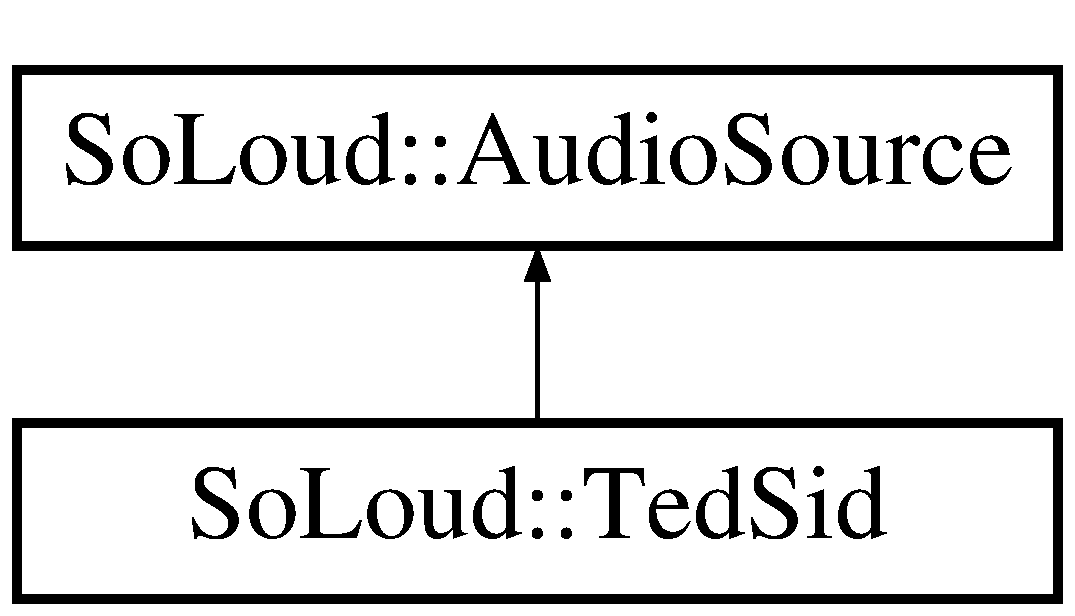
\includegraphics[height=2.000000cm]{class_so_loud_1_1_ted_sid}
\end{center}
\end{figure}
\subsection*{Public Member Functions}
\begin{DoxyCompactItemize}
\item 
\mbox{\Hypertarget{class_so_loud_1_1_ted_sid_a743a333fb6753425fd5a2924075ce218}\label{class_so_loud_1_1_ted_sid_a743a333fb6753425fd5a2924075ce218}} 
result {\bfseries load} (const char $\ast$a\+Filename)
\item 
\mbox{\Hypertarget{class_so_loud_1_1_ted_sid_aef8596ef56e42fe59903dd536116d9bd}\label{class_so_loud_1_1_ted_sid_aef8596ef56e42fe59903dd536116d9bd}} 
result {\bfseries load\+To\+Mem} (const char $\ast$a\+Filename)
\item 
\mbox{\Hypertarget{class_so_loud_1_1_ted_sid_a515322100ddced30984a7d25bb62e2c7}\label{class_so_loud_1_1_ted_sid_a515322100ddced30984a7d25bb62e2c7}} 
result {\bfseries load\+Mem} (unsigned char $\ast$a\+Mem, unsigned int a\+Length, bool a\+Copy=false, bool a\+Take\+Ownership=true)
\item 
\mbox{\Hypertarget{class_so_loud_1_1_ted_sid_a23705859dbe64f44224ac9b8f7648976}\label{class_so_loud_1_1_ted_sid_a23705859dbe64f44224ac9b8f7648976}} 
result {\bfseries load\+File\+To\+Mem} (\mbox{\hyperlink{class_so_loud_1_1_file}{File}} $\ast$a\+File)
\item 
\mbox{\Hypertarget{class_so_loud_1_1_ted_sid_a1de39e8535fedd4a799d7a8a0e5faf69}\label{class_so_loud_1_1_ted_sid_a1de39e8535fedd4a799d7a8a0e5faf69}} 
result {\bfseries load\+File} (\mbox{\hyperlink{class_so_loud_1_1_file}{File}} $\ast$a\+File)
\item 
\mbox{\Hypertarget{class_so_loud_1_1_ted_sid_a968529513936e68677999cc4093202b1}\label{class_so_loud_1_1_ted_sid_a968529513936e68677999cc4093202b1}} 
virtual \mbox{\hyperlink{class_so_loud_1_1_audio_source_instance}{Audio\+Source\+Instance}} $\ast$ {\bfseries create\+Instance} ()
\end{DoxyCompactItemize}
\subsection*{Public Attributes}
\begin{DoxyCompactItemize}
\item 
\mbox{\Hypertarget{class_so_loud_1_1_ted_sid_af02ef0eb966676b1978e701e0289bdd6}\label{class_so_loud_1_1_ted_sid_af02ef0eb966676b1978e701e0289bdd6}} 
\mbox{\hyperlink{class_so_loud_1_1_file}{File}} $\ast$ {\bfseries m\+File}
\item 
\mbox{\Hypertarget{class_so_loud_1_1_ted_sid_a4a0103540e6e109e2373cf02822187cc}\label{class_so_loud_1_1_ted_sid_a4a0103540e6e109e2373cf02822187cc}} 
int {\bfseries m\+Model}
\item 
\mbox{\Hypertarget{class_so_loud_1_1_ted_sid_a9fdc31b3baa994d61c4886c76cd92cf8}\label{class_so_loud_1_1_ted_sid_a9fdc31b3baa994d61c4886c76cd92cf8}} 
bool {\bfseries m\+File\+Owned}
\end{DoxyCompactItemize}
\subsection*{Additional Inherited Members}


The documentation for this class was generated from the following file\+:\begin{DoxyCompactItemize}
\item 
deps/\+E\+S\+A\+T/include/\+E\+S\+A\+T\+\_\+extra/soloud/soloud\+\_\+tedsid.\+h\end{DoxyCompactItemize}

\hypertarget{class_so_loud_1_1_ted_sid_instance}{}\section{So\+Loud\+:\+:Ted\+Sid\+Instance Class Reference}
\label{class_so_loud_1_1_ted_sid_instance}\index{So\+Loud\+::\+Ted\+Sid\+Instance@{So\+Loud\+::\+Ted\+Sid\+Instance}}
Inheritance diagram for So\+Loud\+:\+:Ted\+Sid\+Instance\+:\begin{figure}[H]
\begin{center}
\leavevmode
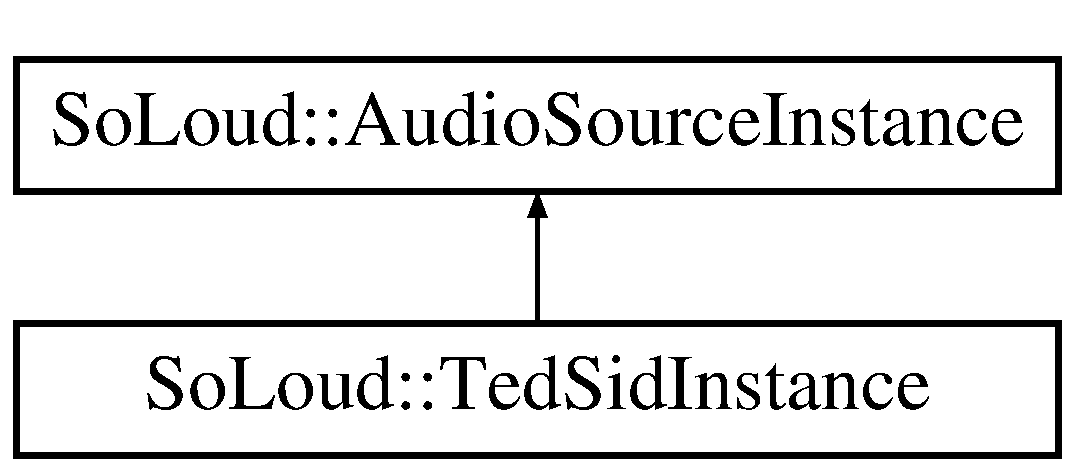
\includegraphics[height=2.000000cm]{class_so_loud_1_1_ted_sid_instance}
\end{center}
\end{figure}
\subsection*{Public Member Functions}
\begin{DoxyCompactItemize}
\item 
\mbox{\Hypertarget{class_so_loud_1_1_ted_sid_instance_a7bd55aaf5d486b3321742dc2f2da9873}\label{class_so_loud_1_1_ted_sid_instance_a7bd55aaf5d486b3321742dc2f2da9873}} 
{\bfseries Ted\+Sid\+Instance} (\mbox{\hyperlink{class_so_loud_1_1_ted_sid}{Ted\+Sid}} $\ast$a\+Parent)
\item 
\mbox{\Hypertarget{class_so_loud_1_1_ted_sid_instance_ae5fa055ffe1872d0f1cba6aae8184820}\label{class_so_loud_1_1_ted_sid_instance_ae5fa055ffe1872d0f1cba6aae8184820}} 
virtual void {\bfseries get\+Audio} (float $\ast$a\+Buffer, unsigned int a\+Samples)
\item 
\mbox{\Hypertarget{class_so_loud_1_1_ted_sid_instance_a75a166390b51bedfb6e6f81b6185604d}\label{class_so_loud_1_1_ted_sid_instance_a75a166390b51bedfb6e6f81b6185604d}} 
virtual void {\bfseries tick} ()
\item 
\mbox{\Hypertarget{class_so_loud_1_1_ted_sid_instance_a471e0e7bdc75af44f7cdbce71a167671}\label{class_so_loud_1_1_ted_sid_instance_a471e0e7bdc75af44f7cdbce71a167671}} 
virtual bool {\bfseries has\+Ended} ()
\item 
\mbox{\Hypertarget{class_so_loud_1_1_ted_sid_instance_a95ec8137ecbd2269147ecb19a02822c6}\label{class_so_loud_1_1_ted_sid_instance_a95ec8137ecbd2269147ecb19a02822c6}} 
virtual float {\bfseries get\+Info} (unsigned int a\+Info\+Key)
\end{DoxyCompactItemize}
\subsection*{Additional Inherited Members}


The documentation for this class was generated from the following file\+:\begin{DoxyCompactItemize}
\item 
deps/\+E\+S\+A\+T/include/\+E\+S\+A\+T\+\_\+extra/soloud/soloud\+\_\+tedsid.\+h\end{DoxyCompactItemize}

\hypertarget{struct_im_gui_text_filter_1_1_text_range}{}\section{Im\+Gui\+Text\+Filter\+:\+:Text\+Range Struct Reference}
\label{struct_im_gui_text_filter_1_1_text_range}\index{Im\+Gui\+Text\+Filter\+::\+Text\+Range@{Im\+Gui\+Text\+Filter\+::\+Text\+Range}}
\subsection*{Public Member Functions}
\begin{DoxyCompactItemize}
\item 
\mbox{\Hypertarget{struct_im_gui_text_filter_1_1_text_range_a4a2b377d4fd141fc3664378041f9f007}\label{struct_im_gui_text_filter_1_1_text_range_a4a2b377d4fd141fc3664378041f9f007}} 
{\bfseries Text\+Range} (const char $\ast$\+\_\+b, const char $\ast$\+\_\+e)
\item 
\mbox{\Hypertarget{struct_im_gui_text_filter_1_1_text_range_ab6b04c316f081e8ad7b044a8afbda63c}\label{struct_im_gui_text_filter_1_1_text_range_ab6b04c316f081e8ad7b044a8afbda63c}} 
const char $\ast$ {\bfseries begin} () const
\item 
\mbox{\Hypertarget{struct_im_gui_text_filter_1_1_text_range_aa5d60286f4c35bfdde82219ff079de9e}\label{struct_im_gui_text_filter_1_1_text_range_aa5d60286f4c35bfdde82219ff079de9e}} 
const char $\ast$ {\bfseries end} () const
\item 
\mbox{\Hypertarget{struct_im_gui_text_filter_1_1_text_range_ab8d74e3b0ce63997746828e4b8ae3bbf}\label{struct_im_gui_text_filter_1_1_text_range_ab8d74e3b0ce63997746828e4b8ae3bbf}} 
bool {\bfseries empty} () const
\item 
\mbox{\Hypertarget{struct_im_gui_text_filter_1_1_text_range_a7d0b405b4db5d33351812b4b3b6e9107}\label{struct_im_gui_text_filter_1_1_text_range_a7d0b405b4db5d33351812b4b3b6e9107}} 
char {\bfseries front} () const
\item 
\mbox{\Hypertarget{struct_im_gui_text_filter_1_1_text_range_aa3bbd8b17b528f548d73c0936228dc85}\label{struct_im_gui_text_filter_1_1_text_range_aa3bbd8b17b528f548d73c0936228dc85}} 
void {\bfseries trim\+\_\+blanks} ()
\item 
\mbox{\Hypertarget{struct_im_gui_text_filter_1_1_text_range_a5854713ee0c08eae73717c6fbe32e34f}\label{struct_im_gui_text_filter_1_1_text_range_a5854713ee0c08eae73717c6fbe32e34f}} 
I\+M\+G\+U\+I\+\_\+\+A\+PI void {\bfseries split} (char separator, \mbox{\hyperlink{class_im_vector}{Im\+Vector}}$<$ \mbox{\hyperlink{struct_im_gui_text_filter_1_1_text_range}{Text\+Range}} $>$ \&out)
\end{DoxyCompactItemize}
\subsection*{Static Public Member Functions}
\begin{DoxyCompactItemize}
\item 
\mbox{\Hypertarget{struct_im_gui_text_filter_1_1_text_range_ad64d136b154a0771109cc31027dae627}\label{struct_im_gui_text_filter_1_1_text_range_ad64d136b154a0771109cc31027dae627}} 
static bool {\bfseries isblank} (char c)
\end{DoxyCompactItemize}
\subsection*{Public Attributes}
\begin{DoxyCompactItemize}
\item 
\mbox{\Hypertarget{struct_im_gui_text_filter_1_1_text_range_a705cf9c8fb0796b3bab9cf20cb18b0ca}\label{struct_im_gui_text_filter_1_1_text_range_a705cf9c8fb0796b3bab9cf20cb18b0ca}} 
const char $\ast$ {\bfseries b}
\item 
\mbox{\Hypertarget{struct_im_gui_text_filter_1_1_text_range_a20daef0e47167d49a017d8f54cb7c607}\label{struct_im_gui_text_filter_1_1_text_range_a20daef0e47167d49a017d8f54cb7c607}} 
const char $\ast$ {\bfseries e}
\end{DoxyCompactItemize}


The documentation for this struct was generated from the following file\+:\begin{DoxyCompactItemize}
\item 
deps/\+E\+S\+A\+T/include/\+E\+S\+A\+T\+\_\+extra/imgui.\+h\end{DoxyCompactItemize}

\hypertarget{struct_e_s_a_t_1_1_vec2}{}\section{E\+S\+AT\+:\+:Vec2 Struct Reference}
\label{struct_e_s_a_t_1_1_vec2}\index{E\+S\+A\+T\+::\+Vec2@{E\+S\+A\+T\+::\+Vec2}}
\subsection*{Public Attributes}
\begin{DoxyCompactItemize}
\item 
\mbox{\Hypertarget{struct_e_s_a_t_1_1_vec2_a2a3e08e024cf00ef8239dc2296c160f9}\label{struct_e_s_a_t_1_1_vec2_a2a3e08e024cf00ef8239dc2296c160f9}} 
float {\bfseries x}
\item 
\mbox{\Hypertarget{struct_e_s_a_t_1_1_vec2_a2796f37aacc7bb77137375eb35c1e877}\label{struct_e_s_a_t_1_1_vec2_a2796f37aacc7bb77137375eb35c1e877}} 
float {\bfseries y}
\end{DoxyCompactItemize}


The documentation for this struct was generated from the following file\+:\begin{DoxyCompactItemize}
\item 
deps/\+E\+S\+A\+T/include/\+E\+S\+A\+T/math.\+h\end{DoxyCompactItemize}

\hypertarget{struct_e_s_a_t_1_1_vec3}{}\section{E\+S\+AT\+:\+:Vec3 Struct Reference}
\label{struct_e_s_a_t_1_1_vec3}\index{E\+S\+A\+T\+::\+Vec3@{E\+S\+A\+T\+::\+Vec3}}
\subsection*{Public Attributes}
\begin{DoxyCompactItemize}
\item 
\mbox{\Hypertarget{struct_e_s_a_t_1_1_vec3_a31f95695776c7f703e1dfe6464f1f272}\label{struct_e_s_a_t_1_1_vec3_a31f95695776c7f703e1dfe6464f1f272}} 
float {\bfseries x}
\item 
\mbox{\Hypertarget{struct_e_s_a_t_1_1_vec3_a0aed8108b15097e8c90af5da4bde41bd}\label{struct_e_s_a_t_1_1_vec3_a0aed8108b15097e8c90af5da4bde41bd}} 
float {\bfseries y}
\item 
\mbox{\Hypertarget{struct_e_s_a_t_1_1_vec3_ab93d7a3e39ad6c5c5186e601559bc8c0}\label{struct_e_s_a_t_1_1_vec3_ab93d7a3e39ad6c5c5186e601559bc8c0}} 
float {\bfseries z}
\end{DoxyCompactItemize}


The documentation for this struct was generated from the following file\+:\begin{DoxyCompactItemize}
\item 
deps/\+E\+S\+A\+T/include/\+E\+S\+A\+T/math.\+h\end{DoxyCompactItemize}

\hypertarget{struct_e_s_a_t_1_1_vec4}{}\section{E\+S\+AT\+:\+:Vec4 Struct Reference}
\label{struct_e_s_a_t_1_1_vec4}\index{E\+S\+A\+T\+::\+Vec4@{E\+S\+A\+T\+::\+Vec4}}
\subsection*{Public Attributes}
\begin{DoxyCompactItemize}
\item 
\mbox{\Hypertarget{struct_e_s_a_t_1_1_vec4_aca0e03c7491084d3875ab811799f171f}\label{struct_e_s_a_t_1_1_vec4_aca0e03c7491084d3875ab811799f171f}} 
float {\bfseries x}
\item 
\mbox{\Hypertarget{struct_e_s_a_t_1_1_vec4_ab17511d03202b058e315b8b6a4a6fb6c}\label{struct_e_s_a_t_1_1_vec4_ab17511d03202b058e315b8b6a4a6fb6c}} 
float {\bfseries y}
\item 
\mbox{\Hypertarget{struct_e_s_a_t_1_1_vec4_a3bc9750b37b2b798e29eb6e347058634}\label{struct_e_s_a_t_1_1_vec4_a3bc9750b37b2b798e29eb6e347058634}} 
float {\bfseries z}
\item 
\mbox{\Hypertarget{struct_e_s_a_t_1_1_vec4_a8330457bca000e2b1bc7be30cd9bf82b}\label{struct_e_s_a_t_1_1_vec4_a8330457bca000e2b1bc7be30cd9bf82b}} 
float {\bfseries w}
\end{DoxyCompactItemize}


The documentation for this struct was generated from the following file\+:\begin{DoxyCompactItemize}
\item 
deps/\+E\+S\+A\+T/include/\+E\+S\+A\+T/math.\+h\end{DoxyCompactItemize}

\hypertarget{struct_vector3}{}\section{Vector3 Struct Reference}
\label{struct_vector3}\index{Vector3@{Vector3}}
\subsection*{Public Attributes}
\begin{DoxyCompactItemize}
\item 
\mbox{\Hypertarget{struct_vector3_a7e2d3237b29a2f29d7b3d8b2934e35f2}\label{struct_vector3_a7e2d3237b29a2f29d7b3d8b2934e35f2}} 
float {\bfseries x}
\item 
\mbox{\Hypertarget{struct_vector3_a86eb35a9fa2d5a49e7fad66a35fa9c13}\label{struct_vector3_a86eb35a9fa2d5a49e7fad66a35fa9c13}} 
float {\bfseries y}
\item 
\mbox{\Hypertarget{struct_vector3_aa8c9461eb24bd2c364258078811a3e9d}\label{struct_vector3_aa8c9461eb24bd2c364258078811a3e9d}} 
float {\bfseries z}
\end{DoxyCompactItemize}


The documentation for this struct was generated from the following file\+:\begin{DoxyCompactItemize}
\item 
deps/common\+\_\+def.\+h\end{DoxyCompactItemize}

\hypertarget{class_so_loud_1_1_vic}{}\section{So\+Loud\+:\+:Vic Class Reference}
\label{class_so_loud_1_1_vic}\index{So\+Loud\+::\+Vic@{So\+Loud\+::\+Vic}}
Inheritance diagram for So\+Loud\+:\+:Vic\+:\begin{figure}[H]
\begin{center}
\leavevmode
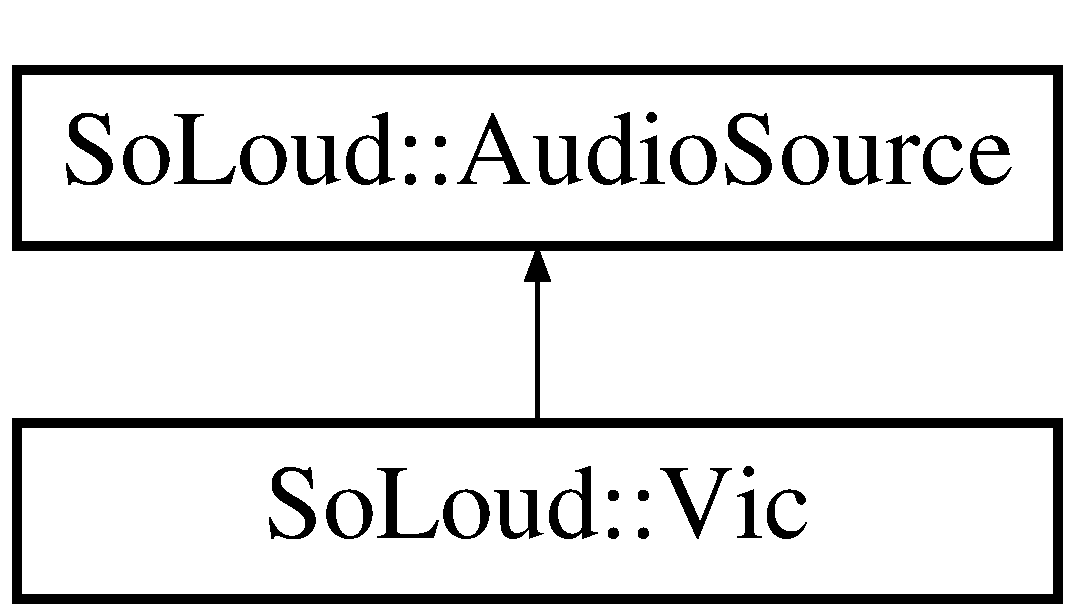
\includegraphics[height=2.000000cm]{class_so_loud_1_1_vic}
\end{center}
\end{figure}
\subsection*{Public Types}
\begin{DoxyCompactItemize}
\item 
\mbox{\Hypertarget{class_so_loud_1_1_vic_aba94fe4e42ee14965eaaf9d40c7e503a}\label{class_so_loud_1_1_vic_aba94fe4e42ee14965eaaf9d40c7e503a}} 
enum \{ {\bfseries P\+AL} = 0, 
{\bfseries N\+T\+SC}
 \}
\item 
\mbox{\Hypertarget{class_so_loud_1_1_vic_a519909c29a5e3fefca3aad5c1c11f1e6}\label{class_so_loud_1_1_vic_a519909c29a5e3fefca3aad5c1c11f1e6}} 
enum \{ \newline
{\bfseries B\+A\+SS} = 0, 
{\bfseries A\+L\+TO}, 
{\bfseries S\+O\+P\+R\+A\+NO}, 
{\bfseries N\+O\+I\+SE}, 
\newline
{\bfseries M\+A\+X\+\_\+\+R\+E\+GS}
 \}
\end{DoxyCompactItemize}
\subsection*{Public Member Functions}
\begin{DoxyCompactItemize}
\item 
\mbox{\Hypertarget{class_so_loud_1_1_vic_a0f50281a9b115fd11b81ee3eb700db79}\label{class_so_loud_1_1_vic_a0f50281a9b115fd11b81ee3eb700db79}} 
void {\bfseries set\+Model} (int model)
\item 
\mbox{\Hypertarget{class_so_loud_1_1_vic_ad2c81766e3858af1800de741002ae928}\label{class_so_loud_1_1_vic_ad2c81766e3858af1800de741002ae928}} 
int {\bfseries get\+Model} () const
\item 
\mbox{\Hypertarget{class_so_loud_1_1_vic_a7ffc185753800ed704512197ad5154e2}\label{class_so_loud_1_1_vic_a7ffc185753800ed704512197ad5154e2}} 
void {\bfseries set\+Register} (int reg, unsigned char value)
\item 
\mbox{\Hypertarget{class_so_loud_1_1_vic_a2039f99f01baa1f86065dd1ca44907ec}\label{class_so_loud_1_1_vic_a2039f99f01baa1f86065dd1ca44907ec}} 
unsigned char {\bfseries get\+Register} (int reg) const
\item 
\mbox{\Hypertarget{class_so_loud_1_1_vic_a057fe9cd48fa0e6e773c153466e94808}\label{class_so_loud_1_1_vic_a057fe9cd48fa0e6e773c153466e94808}} 
virtual \mbox{\hyperlink{class_so_loud_1_1_audio_source_instance}{Audio\+Source\+Instance}} $\ast$ {\bfseries create\+Instance} ()
\end{DoxyCompactItemize}
\subsection*{Friends}
\begin{DoxyCompactItemize}
\item 
\mbox{\Hypertarget{class_so_loud_1_1_vic_a75ba664eca072a2a9a89d338aa6f1789}\label{class_so_loud_1_1_vic_a75ba664eca072a2a9a89d338aa6f1789}} 
class {\bfseries Vic\+Instance}
\end{DoxyCompactItemize}
\subsection*{Additional Inherited Members}


The documentation for this class was generated from the following file\+:\begin{DoxyCompactItemize}
\item 
deps/\+E\+S\+A\+T/include/\+E\+S\+A\+T\+\_\+extra/soloud/soloud\+\_\+vic.\+h\end{DoxyCompactItemize}

\hypertarget{class_so_loud_1_1_vic_instance}{}\section{So\+Loud\+:\+:Vic\+Instance Class Reference}
\label{class_so_loud_1_1_vic_instance}\index{So\+Loud\+::\+Vic\+Instance@{So\+Loud\+::\+Vic\+Instance}}
Inheritance diagram for So\+Loud\+:\+:Vic\+Instance\+:\begin{figure}[H]
\begin{center}
\leavevmode
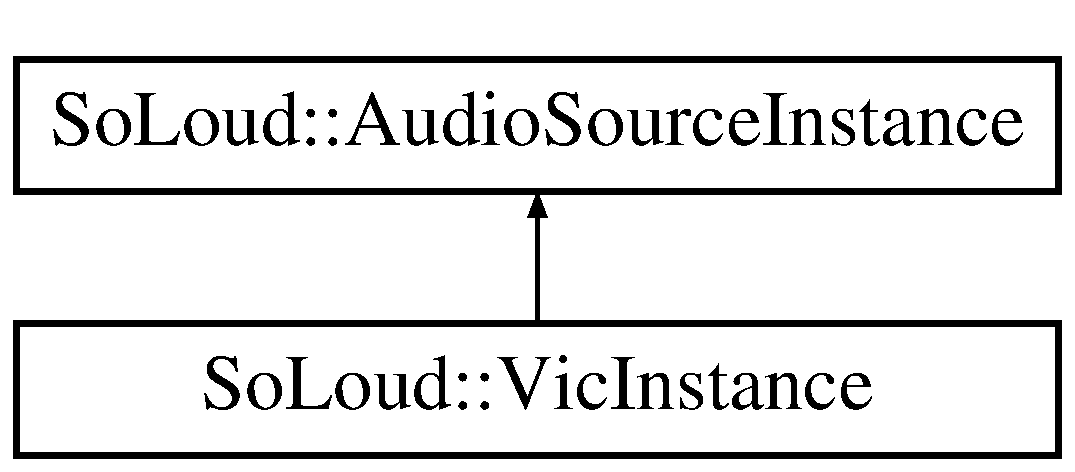
\includegraphics[height=2.000000cm]{class_so_loud_1_1_vic_instance}
\end{center}
\end{figure}
\subsection*{Public Member Functions}
\begin{DoxyCompactItemize}
\item 
\mbox{\Hypertarget{class_so_loud_1_1_vic_instance_ab6ed565589e8f62e1c05cccceb78cbb6}\label{class_so_loud_1_1_vic_instance_ab6ed565589e8f62e1c05cccceb78cbb6}} 
{\bfseries Vic\+Instance} (\mbox{\hyperlink{class_so_loud_1_1_vic}{Vic}} $\ast$a\+Parent)
\item 
\mbox{\Hypertarget{class_so_loud_1_1_vic_instance_a00489f71809080eb25790aa4a9dfbd64}\label{class_so_loud_1_1_vic_instance_a00489f71809080eb25790aa4a9dfbd64}} 
virtual void {\bfseries get\+Audio} (float $\ast$a\+Buffer, unsigned int a\+Samples)
\item 
\mbox{\Hypertarget{class_so_loud_1_1_vic_instance_adf8b06e6a2628e69823b3d31d94245e5}\label{class_so_loud_1_1_vic_instance_adf8b06e6a2628e69823b3d31d94245e5}} 
virtual bool {\bfseries has\+Ended} ()
\end{DoxyCompactItemize}
\subsection*{Additional Inherited Members}


The documentation for this class was generated from the following file\+:\begin{DoxyCompactItemize}
\item 
deps/\+E\+S\+A\+T/include/\+E\+S\+A\+T\+\_\+extra/soloud/soloud\+\_\+vic.\+h\end{DoxyCompactItemize}

\hypertarget{class_so_loud_1_1_wav}{}\section{So\+Loud\+:\+:Wav Class Reference}
\label{class_so_loud_1_1_wav}\index{So\+Loud\+::\+Wav@{So\+Loud\+::\+Wav}}
Inheritance diagram for So\+Loud\+:\+:Wav\+:\begin{figure}[H]
\begin{center}
\leavevmode
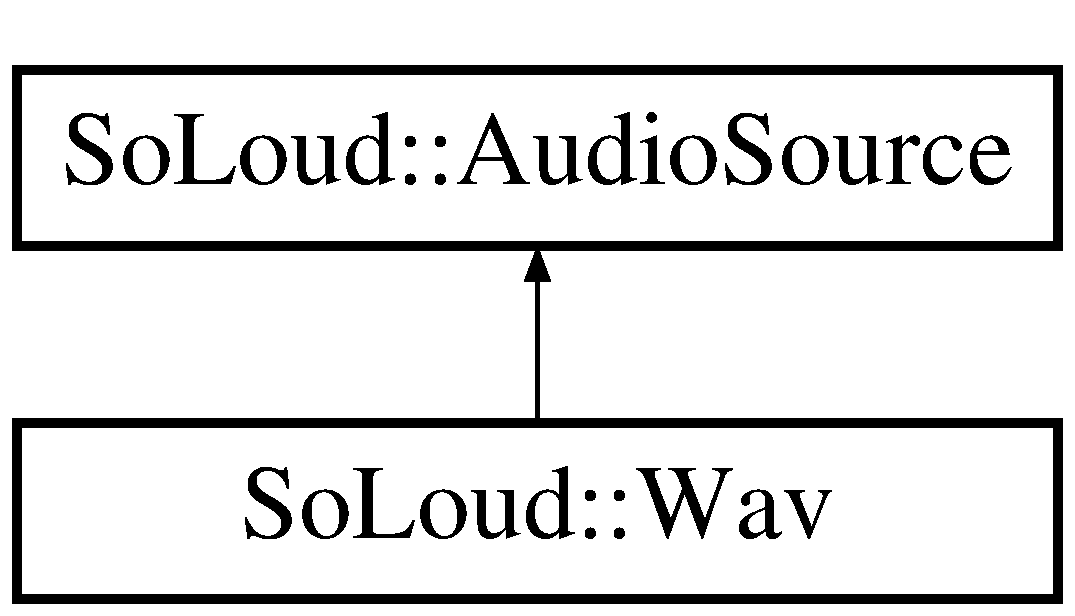
\includegraphics[height=2.000000cm]{class_so_loud_1_1_wav}
\end{center}
\end{figure}
\subsection*{Public Member Functions}
\begin{DoxyCompactItemize}
\item 
\mbox{\Hypertarget{class_so_loud_1_1_wav_aede2b2cea88eec6b9baa81dc503eeb42}\label{class_so_loud_1_1_wav_aede2b2cea88eec6b9baa81dc503eeb42}} 
result {\bfseries load} (const char $\ast$a\+Filename)
\item 
\mbox{\Hypertarget{class_so_loud_1_1_wav_a9844134680e0580fc9bce78aa8923a0b}\label{class_so_loud_1_1_wav_a9844134680e0580fc9bce78aa8923a0b}} 
result {\bfseries load\+Mem} (unsigned char $\ast$a\+Mem, unsigned int a\+Length, bool a\+Copy=false, bool a\+Take\+Ownership=true)
\item 
\mbox{\Hypertarget{class_so_loud_1_1_wav_a79d1999bf6b95de7f284d45fc126537f}\label{class_so_loud_1_1_wav_a79d1999bf6b95de7f284d45fc126537f}} 
result {\bfseries load\+File} (\mbox{\hyperlink{class_so_loud_1_1_file}{File}} $\ast$a\+File)
\item 
\mbox{\Hypertarget{class_so_loud_1_1_wav_aabd5ef0f446202e392d7acab433c26c6}\label{class_so_loud_1_1_wav_aabd5ef0f446202e392d7acab433c26c6}} 
virtual \mbox{\hyperlink{class_so_loud_1_1_audio_source_instance}{Audio\+Source\+Instance}} $\ast$ {\bfseries create\+Instance} ()
\item 
\mbox{\Hypertarget{class_so_loud_1_1_wav_a89b7a8b1041139e0ed8b9a81b17626ed}\label{class_so_loud_1_1_wav_a89b7a8b1041139e0ed8b9a81b17626ed}} 
time {\bfseries get\+Length} ()
\end{DoxyCompactItemize}
\subsection*{Public Attributes}
\begin{DoxyCompactItemize}
\item 
\mbox{\Hypertarget{class_so_loud_1_1_wav_a9c1c69df5dde076641f92d6553f3db38}\label{class_so_loud_1_1_wav_a9c1c69df5dde076641f92d6553f3db38}} 
float $\ast$ {\bfseries m\+Data}
\item 
\mbox{\Hypertarget{class_so_loud_1_1_wav_ac0cbf7aeb7bdcd19e2d2da58117c4ea3}\label{class_so_loud_1_1_wav_ac0cbf7aeb7bdcd19e2d2da58117c4ea3}} 
unsigned int {\bfseries m\+Sample\+Count}
\end{DoxyCompactItemize}
\subsection*{Additional Inherited Members}


The documentation for this class was generated from the following file\+:\begin{DoxyCompactItemize}
\item 
deps/\+E\+S\+A\+T/include/\+E\+S\+A\+T\+\_\+extra/soloud/soloud\+\_\+wav.\+h\end{DoxyCompactItemize}

\hypertarget{class_so_loud_1_1_wav_instance}{}\section{So\+Loud\+:\+:Wav\+Instance Class Reference}
\label{class_so_loud_1_1_wav_instance}\index{So\+Loud\+::\+Wav\+Instance@{So\+Loud\+::\+Wav\+Instance}}
Inheritance diagram for So\+Loud\+:\+:Wav\+Instance\+:\begin{figure}[H]
\begin{center}
\leavevmode
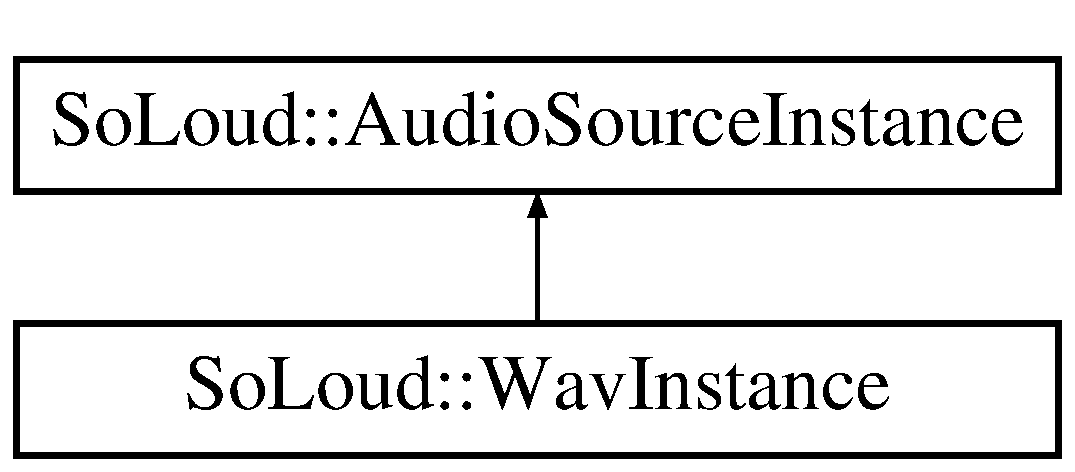
\includegraphics[height=2.000000cm]{class_so_loud_1_1_wav_instance}
\end{center}
\end{figure}
\subsection*{Public Member Functions}
\begin{DoxyCompactItemize}
\item 
\mbox{\Hypertarget{class_so_loud_1_1_wav_instance_ab647cc457e7203c4831321e5675881a7}\label{class_so_loud_1_1_wav_instance_ab647cc457e7203c4831321e5675881a7}} 
{\bfseries Wav\+Instance} (\mbox{\hyperlink{class_so_loud_1_1_wav}{Wav}} $\ast$a\+Parent)
\item 
\mbox{\Hypertarget{class_so_loud_1_1_wav_instance_a1d138f3fee5b2f82febd5bafc721c016}\label{class_so_loud_1_1_wav_instance_a1d138f3fee5b2f82febd5bafc721c016}} 
virtual void {\bfseries get\+Audio} (float $\ast$a\+Buffer, unsigned int a\+Samples)
\item 
\mbox{\Hypertarget{class_so_loud_1_1_wav_instance_a57c4a74f8321ff60b110aef7f853776b}\label{class_so_loud_1_1_wav_instance_a57c4a74f8321ff60b110aef7f853776b}} 
virtual result {\bfseries rewind} ()
\item 
\mbox{\Hypertarget{class_so_loud_1_1_wav_instance_ade8f8939a431a779743c8b72e3f10592}\label{class_so_loud_1_1_wav_instance_ade8f8939a431a779743c8b72e3f10592}} 
virtual bool {\bfseries has\+Ended} ()
\end{DoxyCompactItemize}
\subsection*{Additional Inherited Members}


The documentation for this class was generated from the following file\+:\begin{DoxyCompactItemize}
\item 
deps/\+E\+S\+A\+T/include/\+E\+S\+A\+T\+\_\+extra/soloud/soloud\+\_\+wav.\+h\end{DoxyCompactItemize}

\hypertarget{class_so_loud_1_1_wav_stream}{}\section{So\+Loud\+:\+:Wav\+Stream Class Reference}
\label{class_so_loud_1_1_wav_stream}\index{So\+Loud\+::\+Wav\+Stream@{So\+Loud\+::\+Wav\+Stream}}
Inheritance diagram for So\+Loud\+:\+:Wav\+Stream\+:\begin{figure}[H]
\begin{center}
\leavevmode
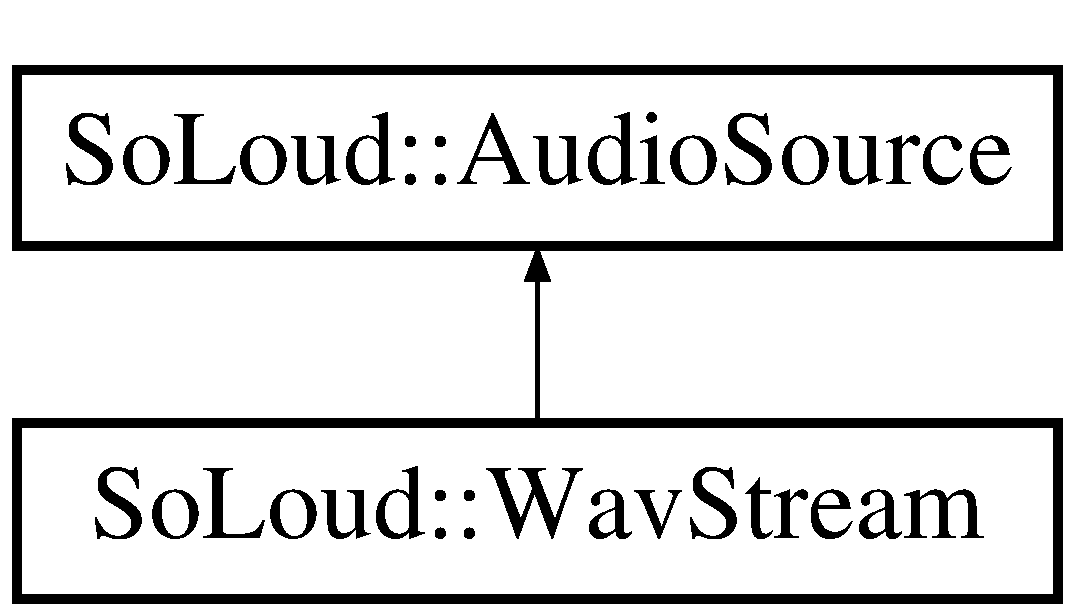
\includegraphics[height=2.000000cm]{class_so_loud_1_1_wav_stream}
\end{center}
\end{figure}
\subsection*{Public Member Functions}
\begin{DoxyCompactItemize}
\item 
\mbox{\Hypertarget{class_so_loud_1_1_wav_stream_a773cedad6f1633b4eb82594147964ca1}\label{class_so_loud_1_1_wav_stream_a773cedad6f1633b4eb82594147964ca1}} 
result {\bfseries load} (const char $\ast$a\+Filename)
\item 
\mbox{\Hypertarget{class_so_loud_1_1_wav_stream_a14bbfdad0390548cea4bb6dd2a5339f8}\label{class_so_loud_1_1_wav_stream_a14bbfdad0390548cea4bb6dd2a5339f8}} 
result {\bfseries load\+Mem} (unsigned char $\ast$a\+Data, unsigned int a\+Data\+Len, bool a\+Copy=false, bool a\+Take\+Ownership=true)
\item 
\mbox{\Hypertarget{class_so_loud_1_1_wav_stream_a03f942b0777845f796a72164bdd88f24}\label{class_so_loud_1_1_wav_stream_a03f942b0777845f796a72164bdd88f24}} 
result {\bfseries load\+To\+Mem} (const char $\ast$a\+Filename)
\item 
\mbox{\Hypertarget{class_so_loud_1_1_wav_stream_a82ed0d1c2d46674af996dacda3476f14}\label{class_so_loud_1_1_wav_stream_a82ed0d1c2d46674af996dacda3476f14}} 
result {\bfseries load\+File} (\mbox{\hyperlink{class_so_loud_1_1_file}{File}} $\ast$a\+File)
\item 
\mbox{\Hypertarget{class_so_loud_1_1_wav_stream_a4ae9a4f93ae01b753be32723fd3ebd8a}\label{class_so_loud_1_1_wav_stream_a4ae9a4f93ae01b753be32723fd3ebd8a}} 
result {\bfseries load\+File\+To\+Mem} (\mbox{\hyperlink{class_so_loud_1_1_file}{File}} $\ast$a\+File)
\item 
\mbox{\Hypertarget{class_so_loud_1_1_wav_stream_a04a870fc47575ae432ed14d98bcf2470}\label{class_so_loud_1_1_wav_stream_a04a870fc47575ae432ed14d98bcf2470}} 
virtual \mbox{\hyperlink{class_so_loud_1_1_audio_source_instance}{Audio\+Source\+Instance}} $\ast$ {\bfseries create\+Instance} ()
\item 
\mbox{\Hypertarget{class_so_loud_1_1_wav_stream_a31e52783f116e35a9556de2bb0bbc21e}\label{class_so_loud_1_1_wav_stream_a31e52783f116e35a9556de2bb0bbc21e}} 
time {\bfseries get\+Length} ()
\item 
\mbox{\Hypertarget{class_so_loud_1_1_wav_stream_a51f8c2a96dc01eec1c614a0a4a165bdf}\label{class_so_loud_1_1_wav_stream_a51f8c2a96dc01eec1c614a0a4a165bdf}} 
result {\bfseries parse} (\mbox{\hyperlink{class_so_loud_1_1_file}{File}} $\ast$a\+File)
\end{DoxyCompactItemize}
\subsection*{Public Attributes}
\begin{DoxyCompactItemize}
\item 
\mbox{\Hypertarget{class_so_loud_1_1_wav_stream_a2dcf2c2ca18a7002c508628a470b55cd}\label{class_so_loud_1_1_wav_stream_a2dcf2c2ca18a7002c508628a470b55cd}} 
int {\bfseries m\+Ogg}
\item 
\mbox{\Hypertarget{class_so_loud_1_1_wav_stream_abb044202f928f511f5b8904ea5372915}\label{class_so_loud_1_1_wav_stream_abb044202f928f511f5b8904ea5372915}} 
char $\ast$ {\bfseries m\+Filename}
\item 
\mbox{\Hypertarget{class_so_loud_1_1_wav_stream_ac6accb9a54740f5f5b4a7931cb880d61}\label{class_so_loud_1_1_wav_stream_ac6accb9a54740f5f5b4a7931cb880d61}} 
\mbox{\hyperlink{class_so_loud_1_1_file}{File}} $\ast$ {\bfseries m\+Mem\+File}
\item 
\mbox{\Hypertarget{class_so_loud_1_1_wav_stream_adf01b657b07d0d0e2a26303998f02b02}\label{class_so_loud_1_1_wav_stream_adf01b657b07d0d0e2a26303998f02b02}} 
\mbox{\hyperlink{class_so_loud_1_1_file}{File}} $\ast$ {\bfseries m\+Stream\+File}
\item 
\mbox{\Hypertarget{class_so_loud_1_1_wav_stream_adf75d044bb547cd1b59b9d4e7774cd45}\label{class_so_loud_1_1_wav_stream_adf75d044bb547cd1b59b9d4e7774cd45}} 
unsigned int {\bfseries m\+Data\+Offset}
\item 
\mbox{\Hypertarget{class_so_loud_1_1_wav_stream_aaaaa9cda642e41dc71c3041994803264}\label{class_so_loud_1_1_wav_stream_aaaaa9cda642e41dc71c3041994803264}} 
unsigned int {\bfseries m\+Bits}
\item 
\mbox{\Hypertarget{class_so_loud_1_1_wav_stream_a2437070c8bbdee98c3bc12380ed4f81f}\label{class_so_loud_1_1_wav_stream_a2437070c8bbdee98c3bc12380ed4f81f}} 
unsigned int {\bfseries m\+Sample\+Count}
\end{DoxyCompactItemize}
\subsection*{Additional Inherited Members}


The documentation for this class was generated from the following file\+:\begin{DoxyCompactItemize}
\item 
deps/\+E\+S\+A\+T/include/\+E\+S\+A\+T\+\_\+extra/soloud/soloud\+\_\+wavstream.\+h\end{DoxyCompactItemize}

\hypertarget{class_so_loud_1_1_wav_stream_instance}{}\section{So\+Loud\+:\+:Wav\+Stream\+Instance Class Reference}
\label{class_so_loud_1_1_wav_stream_instance}\index{So\+Loud\+::\+Wav\+Stream\+Instance@{So\+Loud\+::\+Wav\+Stream\+Instance}}
Inheritance diagram for So\+Loud\+:\+:Wav\+Stream\+Instance\+:\begin{figure}[H]
\begin{center}
\leavevmode
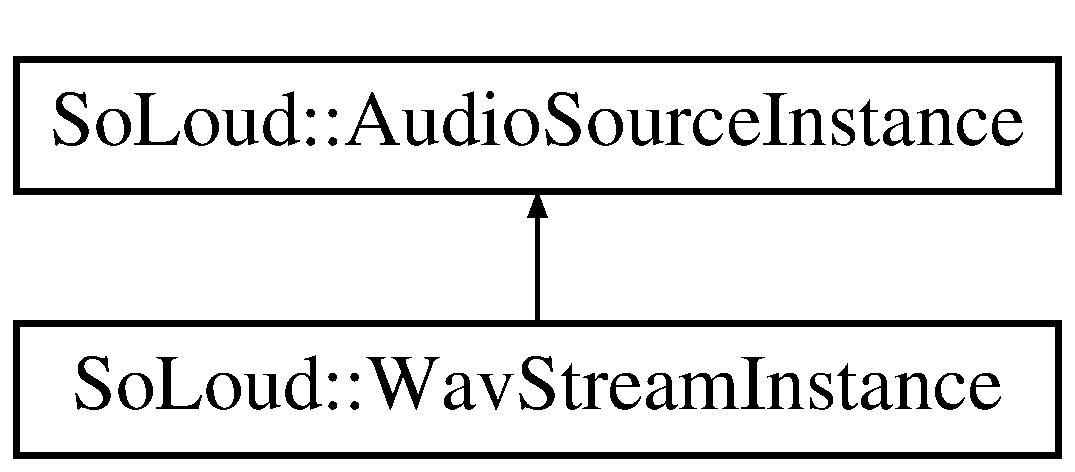
\includegraphics[height=2.000000cm]{class_so_loud_1_1_wav_stream_instance}
\end{center}
\end{figure}
\subsection*{Public Member Functions}
\begin{DoxyCompactItemize}
\item 
\mbox{\Hypertarget{class_so_loud_1_1_wav_stream_instance_a2c28700b138633763722906d90a27b87}\label{class_so_loud_1_1_wav_stream_instance_a2c28700b138633763722906d90a27b87}} 
{\bfseries Wav\+Stream\+Instance} (\mbox{\hyperlink{class_so_loud_1_1_wav_stream}{Wav\+Stream}} $\ast$a\+Parent)
\item 
\mbox{\Hypertarget{class_so_loud_1_1_wav_stream_instance_a860ab1646c7e9f86474993e7f6e246b6}\label{class_so_loud_1_1_wav_stream_instance_a860ab1646c7e9f86474993e7f6e246b6}} 
virtual void {\bfseries get\+Audio} (float $\ast$a\+Buffer, unsigned int a\+Samples)
\item 
\mbox{\Hypertarget{class_so_loud_1_1_wav_stream_instance_a61573538b0e0b69a3b21fd394d1b7090}\label{class_so_loud_1_1_wav_stream_instance_a61573538b0e0b69a3b21fd394d1b7090}} 
virtual result {\bfseries rewind} ()
\item 
\mbox{\Hypertarget{class_so_loud_1_1_wav_stream_instance_a3bfe7d52821a15b46a537ed17367c900}\label{class_so_loud_1_1_wav_stream_instance_a3bfe7d52821a15b46a537ed17367c900}} 
virtual bool {\bfseries has\+Ended} ()
\end{DoxyCompactItemize}
\subsection*{Additional Inherited Members}


The documentation for this class was generated from the following file\+:\begin{DoxyCompactItemize}
\item 
deps/\+E\+S\+A\+T/include/\+E\+S\+A\+T\+\_\+extra/soloud/soloud\+\_\+wavstream.\+h\end{DoxyCompactItemize}

\chapter{File Documentation}
\hypertarget{path_8h}{}\section{include/path.h File Reference}
\label{path_8h}\index{include/path.\+h@{include/path.\+h}}


Class to construct and walk trough a path.  


{\ttfamily \#include \char`\"{}platform\+\_\+types.\+h\char`\"{}}\newline
{\ttfamily \#include \char`\"{}common\+\_\+def.\+h\char`\"{}}\newline
\subsection*{Classes}
\begin{DoxyCompactItemize}
\item 
class \mbox{\hyperlink{class_path}{Path}}
\begin{DoxyCompactList}\small\item\em \mbox{\hyperlink{class_path}{Path}} class. \end{DoxyCompactList}\end{DoxyCompactItemize}
\subsection*{Enumerations}
\begin{DoxyCompactItemize}
\item 
\mbox{\Hypertarget{path_8h_a224b9163917ac32fc95a60d8c1eec3aa}\label{path_8h_a224b9163917ac32fc95a60d8c1eec3aa}} 
enum {\bfseries Direction} \{ {\bfseries k\+Dir\+None} = -\/1, 
{\bfseries k\+Dir\+Forward} = 0
 \}
\item 
\mbox{\Hypertarget{path_8h_a8bb1ef53467e4f61410d12822d922498}\label{path_8h_a8bb1ef53467e4f61410d12822d922498}} 
enum {\bfseries Action} \{ {\bfseries k\+Action\+None} = -\/1, 
{\bfseries k\+Action\+Straight} = 0, 
{\bfseries k\+Action\+Loop\+N\+Times}, 
{\bfseries k\+Action\+Loop\+Infinite}
 \}
\end{DoxyCompactItemize}
\subsection*{Variables}
\begin{DoxyCompactItemize}
\item 
\mbox{\Hypertarget{path_8h_a11cfdf40d0579a3998ee9d89ac253d56}\label{path_8h_a11cfdf40d0579a3998ee9d89ac253d56}} 
const int {\bfseries k\+Max\+Points} = 500
\end{DoxyCompactItemize}


\subsection{Detailed Description}
Class to construct and walk trough a path. 

Toni Barella Artificial Intelligence -\/ 3\+H\+ND E\+S\+AT 2016 -\/ 2019

Jose Maria Martinez 
%--- End generated contents ---

% Index
\backmatter
\newpage
\phantomsection
\clearemptydoublepage
\addcontentsline{toc}{chapter}{Index}
\printindex

\end{document}
